
\section{\ref{PS:Q:Performance}}

\textit{Can we create a solution that scales such that the number of turbines does not impact the regulation cycle time?}

\subsection{Experiments}
\label{sec:Exper:perfom}

%Scalability is by Bondi\cite{Bondi:2000:CSI:350391.350432} defined as \textit{the systems ability to accommodate an increasing number of elements or objects, to process growing volumes of work gracefully, and/or to be susceptible to enlargement}.

The \ref{PS:Q:Performance} problem address if the proposed decentralized solution is able to keep a constant regulation cycle time independent from the number of turbines. This problem operates in a 3-dimensional space with regulation cycle time (ms), number of cache reads and number of turbines as parameters. To study the correlation between the parameters, we isolate two parameters by making the third constant.

Thus to fully address \ref{PS:Q:Performance} this experiment has been divided into two experiments:
 
\begin{description}
	\item[Experiment 1] aims to investigate the anti-correlation between the implemented sleep time of the regulation cycle and the number of cache reads for the decentralized system. This is relevant because changing the sleep time is expected to impact the number of cache reads, since an increase in sleep time increases the time Connext has to overwrite received states, thus decreasing the number of cache reads (as explained in \cref{sec:cachereads}). Thus the constant for this is experiment is the number of turbines.
	\item[Experiment 2] aims to investigate the impact on the regulation cycle time and the number of cache reads when increasing the number of turbines in the decentralized solution, and thus answer the \ref{PS:Q:Performance} problem. The constant for this experiment is the sleep time.
\end{description}

The cycle regulation time of the decentralized solution is defined as the difference between the receive timestamp of the oldest turbine state(tOldestState) received and the timestamp sampled right after, a new turbine state has been sent (tSent) (as illustrated on \cref{fig:timingDecentral}):

$$regulation~cycle~time=tSent-tOldestState$$

\begin{figure}[b]
	\input{figures/tikz/timingDiagramDecntral}
	\caption{Decentralized regulation time}
	\label{fig:timingDecentral}
\end{figure}

The timestamp of the oldest turbine state is used to include network traffic in the regulation cycle time, as opposed to just sampling the time locally. Thus, if the decentralized solution is using cached data this will be reflected in the regulation cycle time. Note that by this definition, it is possible for regulation cycle time to be lower than the sleep time, even though the sleep operation is a part of the regulation cycle. 


\subsection{Experiment 1: How sleep time impacts the regulation cycle time and the number of cache reads}
\label{subsec:Exper:perfom:1}
The purpose of this experiment is to show how the sleep time affects the number of cache reads and the regulation cycle time for the decentralized solution (see \cref{sec:cachereads} for cache reads description).  
The experiment is performed with cycle time t=\testCycletimeNumbers.  

The following procedure is used each time the experiment is performed:
\begin{enumerate}
	\item Start the system with a cycle time of t ms and 50 turbines.
	\item Make sure the system is stable.
	\item Start logging the regulation cycle time and the number of cache reads.
	\item Stop logging after 50 seconds.
\end{enumerate}

50 seconds of logging provided 59000 data samples as the lowest amount of data samples for a single data set (the data set using 50 ms sleep time). Thus each data set of this experiment has been plotted using 59000 data samples.

\subsection{Experiment 2: How the number of turbines impacts the regulation cycle time and the number of cache reads}
\label{subsec:Exper:perfom:2}
The purpose of this experiment is to answer the \ref{PS:Q:Performance} problem, by showing how the number of turbines affects the regulation cycle time for the decentralized solution. To complete the picture we also investigate how the number of turbines affects the cache reads, since an expected side effect of increasing the number of turbines also increases the number of cache reads as described in \cref{sec:cachereads}.

The experiments are performed with n=\testTurbineNumbers ~turbines. The sleep time is set to 20 ms and is constant for this experiment.

The test system is expected to be running only one instance in a real life implementation, therefore the machine logging the data will only run one instance and the supporting machines will run the rest, generating system load.

The following procedure is used each time the experiment is performed:
\begin{enumerate}
	\item Start the system with n turbines.
	\item Make sure the system is stable.
	\item Start logging the reported regulation run time and the number of cache reads.
	\item Stop logging after 50 seconds.
\end{enumerate}

50 seconds of logging provided 14500 data samples as the lowest amount of data samples for a single data set (the data using 5 turbines). Thus each data set of this experiment has been plotted using 14500 data samples.

\subsection{Results} \label{sec:exp:performance}

We use the following box plot type (for \cref{fig:exp:decen:sleep} and \cref{fig:exp:decen:turbines}): The central mark is the median, the edges of the box are the 25th and 75th percentiles, the whiskers extend to the most extreme data points not considered outliers, and outliers are plotted individually. The whisker length is denoted as 1.5 IQR. 

\subsubsection{\nameref{subsec:Exper:perfom:1}}

\begin{figure}[h!]
	\centering
%	\begin{tikzpicture}
\begin{axis}
[
width=\resultsPlotWidthScale\textwidth,
axis y line*=left,
xlabel=Wait time (ms),
ylabel=Regulation cycle time (ms),
ymin = 0,  ymax = 80,
xtick={1, 2, 3, 4, 5, 6, 7, 8, 9},
xticklabels={10, 15, 20, 25, 30, 35, 40, 45, 50},
boxplot/draw direction=y,
ymajorgrids=true,
yminorgrids=true,
minor y tick num=1
]

%% /home/stefan/work/TestResults/Test6_Decentralized_12-7-2014_1327/nCycleTime/DecentralizedLog1.csv
\buildBoxPlot{10.578002}{15.286001}{9.942}{148.911}{0.415002}

%% /home/stefan/work/TestResults/Test6_Decentralized_12-7-2014_1327/nCycleTime/DecentralizedLog2.csv
\buildBoxPlot{15.026002}{15.383002}{14.312002}{26.729001}{1.379}

%% /home/stefan/work/TestResults/Test6_Decentralized_12-7-2014_1327/nCycleTime/DecentralizedLog3.csv
\buildBoxPlot{19.926}{20.380001}{18.979001}{29.932002}{0.435}

%% /home/stefan/work/TestResults/Test6_Decentralized_12-7-2014_1327/nCycleTime/DecentralizedLog4.csv
\buildBoxPlot{25.079001}{25.322}{24.637001}{32.794001}{12.225002}

%% /home/stefan/work/TestResults/Test6_Decentralized_12-7-2014_1327/nCycleTime/DecentralizedLog5.csv
\buildBoxPlot{30.099}{30.363}{29.565001}{42.436}{4.466}

%% /home/stefan/work/TestResults/Test6_Decentralized_12-7-2014_1327/nCycleTime/DecentralizedLog6.csv
\buildBoxPlot{35.153001}{35.328002}{34.853001}{45.836001}{10.347}

%% /home/stefan/work/TestResults/Test6_Decentralized_12-7-2014_1327/nCycleTime/DecentralizedLog7.csv
\buildBoxPlot{40.157001}{40.434001}{39.626}{58.338001}{6.398001}

%% /home/stefan/work/TestResults/Test6_Decentralized_12-7-2014_1327/nCycleTime/DecentralizedLog8.csv
\buildBoxPlot{45.185}{45.330001}{44.928002}{50.089}{29.313}

%% /home/stefan/work/TestResults/Test6_Decentralized_12-7-2014_1327/nCycleTime/DecentralizedLog9.csv
\buildBoxPlot{49.958002}{50.391001}{49.019}{64.611002}{4.846}


\addplot[thick, red!70] coordinates {
	(1 ,10.578002)
	(2 ,15.026002)
	(3 ,19.926)
	(4 ,25.079001)
	(5 ,30.099)
	(6 ,35.153001)
	(7 ,40.157001)
	(8 ,45.185)
	(9 ,49.958002)
};

\end{axis}
\end{tikzpicture}

	% This file was created by matlab2tikz.
% Minimal pgfplots version: 1.3
%
%The latest updates can be retrieved from
%  http://www.mathworks.com/matlabcentral/fileexchange/22022-matlab2tikz
%where you can also make suggestions and rate matlab2tikz.
%
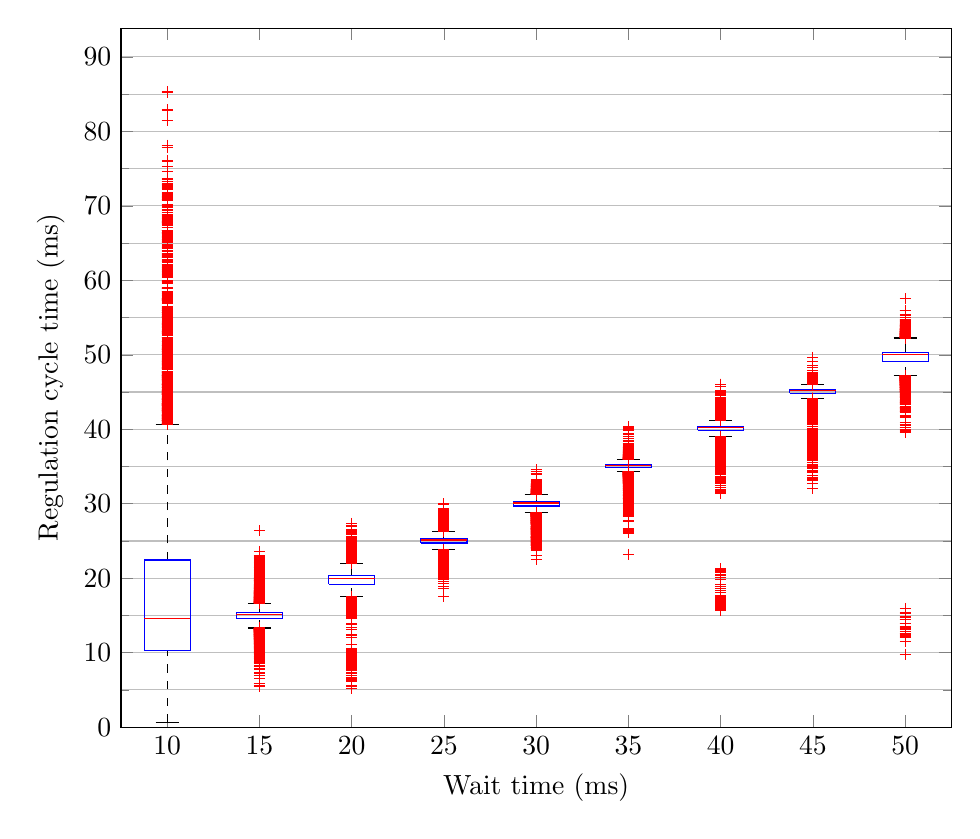
\begin{tikzpicture}

\begin{axis}[%
	width=\resultsPlotWidthScale\textwidth,
	xmin=0.5,
	xmax=9.5,
	ymin=0,
	xlabel=Wait time (ms),
	ylabel=Regulation cycle time (ms),
	xtick={1, 2, 3, 4, 5, 6, 7, 8, 9},
	xticklabels={10, 15, 20, 25, 30, 35, 40, 45, 50},
	ymajorgrids=true,
	yminorgrids=true,
	minor y tick num=1
]
\addplot [color=black,dashed,forget plot]
  table[row sep=crcr]{%
1 22.4525015\\
1 40.601\\
};
\addplot [color=black,dashed,forget plot]
  table[row sep=crcr]{%
2 15.386001\\
2 16.628001\\
};
\addplot [color=black,dashed,forget plot]
  table[row sep=crcr]{%
3 20.328002\\
3 21.995001\\
};
\addplot [color=black,dashed,forget plot]
  table[row sep=crcr]{%
4 25.350001\\
4 26.279001\\
};
\addplot [color=black,dashed,forget plot]
  table[row sep=crcr]{%
5 30.312001\\
5 31.219001\\
};
\addplot [color=black,dashed,forget plot]
  table[row sep=crcr]{%
6 35.315001\\
6 35.919001\\
};
\addplot [color=black,dashed,forget plot]
  table[row sep=crcr]{%
7 40.380501\\
7 41.197\\
};
\addplot [color=black,dashed,forget plot]
  table[row sep=crcr]{%
8 45.316001\\
8 46.006001\\
};
\addplot [color=black,dashed,forget plot]
  table[row sep=crcr]{%
9 50.356\\
9 52.254001\\
};
\addplot [color=black,dashed,forget plot]
  table[row sep=crcr]{%
1 0.623001\\
1 10.3525005\\
};
\addplot [color=black,dashed,forget plot]
  table[row sep=crcr]{%
2 13.316001\\
2 14.558\\
};
\addplot [color=black,dashed,forget plot]
  table[row sep=crcr]{%
3 17.548001\\
3 19.215501\\
};
\addplot [color=black,dashed,forget plot]
  table[row sep=crcr]{%
4 23.8\\
4 24.73\\
};
\addplot [color=black,dashed,forget plot]
  table[row sep=crcr]{%
5 28.793002\\
5 29.704001\\
};
\addplot [color=black,dashed,forget plot]
  table[row sep=crcr]{%
6 34.306001\\
6 34.9110015\\
};
\addplot [color=black,dashed,forget plot]
  table[row sep=crcr]{%
7 39.023\\
7 39.836\\
};
\addplot [color=black,dashed,forget plot]
  table[row sep=crcr]{%
8 44.166001\\
8 44.855501\\
};
\addplot [color=black,dashed,forget plot]
  table[row sep=crcr]{%
9 47.193001\\
9 49.09\\
};
\addplot [color=black,solid,forget plot]
  table[row sep=crcr]{%
0.875 40.601\\
1.125 40.601\\
};
\addplot [color=black,solid,forget plot]
  table[row sep=crcr]{%
1.875 16.628001\\
2.125 16.628001\\
};
\addplot [color=black,solid,forget plot]
  table[row sep=crcr]{%
2.875 21.995001\\
3.125 21.995001\\
};
\addplot [color=black,solid,forget plot]
  table[row sep=crcr]{%
3.875 26.279001\\
4.125 26.279001\\
};
\addplot [color=black,solid,forget plot]
  table[row sep=crcr]{%
4.875 31.219001\\
5.125 31.219001\\
};
\addplot [color=black,solid,forget plot]
  table[row sep=crcr]{%
5.875 35.919001\\
6.125 35.919001\\
};
\addplot [color=black,solid,forget plot]
  table[row sep=crcr]{%
6.875 41.197\\
7.125 41.197\\
};
\addplot [color=black,solid,forget plot]
  table[row sep=crcr]{%
7.875 46.006001\\
8.125 46.006001\\
};
\addplot [color=black,solid,forget plot]
  table[row sep=crcr]{%
8.875 52.254001\\
9.125 52.254001\\
};
\addplot [color=black,solid,forget plot]
  table[row sep=crcr]{%
0.875 0.623001\\
1.125 0.623001\\
};
\addplot [color=black,solid,forget plot]
  table[row sep=crcr]{%
1.875 13.316001\\
2.125 13.316001\\
};
\addplot [color=black,solid,forget plot]
  table[row sep=crcr]{%
2.875 17.548001\\
3.125 17.548001\\
};
\addplot [color=black,solid,forget plot]
  table[row sep=crcr]{%
3.875 23.8\\
4.125 23.8\\
};
\addplot [color=black,solid,forget plot]
  table[row sep=crcr]{%
4.875 28.793002\\
5.125 28.793002\\
};
\addplot [color=black,solid,forget plot]
  table[row sep=crcr]{%
5.875 34.306001\\
6.125 34.306001\\
};
\addplot [color=black,solid,forget plot]
  table[row sep=crcr]{%
6.875 39.023\\
7.125 39.023\\
};
\addplot [color=black,solid,forget plot]
  table[row sep=crcr]{%
7.875 44.166001\\
8.125 44.166001\\
};
\addplot [color=black,solid,forget plot]
  table[row sep=crcr]{%
8.875 47.193001\\
9.125 47.193001\\
};
\addplot [color=blue,solid,forget plot]
  table[row sep=crcr]{%
0.75  10.3525005\\
0.75  22.4525015\\
1.25  22.4525015\\
1.25  10.3525005\\
0.75  10.3525005\\
};
\addplot [color=blue,solid,forget plot]
  table[row sep=crcr]{%
1.75  14.558\\
1.75  15.386001\\
2.25  15.386001\\
2.25  14.558\\
1.75  14.558\\
};
\addplot [color=blue,solid,forget plot]
  table[row sep=crcr]{%
2.75  19.215501\\
2.75  20.328002\\
3.25  20.328002\\
3.25  19.215501\\
2.75  19.215501\\
};
\addplot [color=blue,solid,forget plot]
  table[row sep=crcr]{%
3.75  24.73\\
3.75  25.350001\\
4.25  25.350001\\
4.25  24.73\\
3.75  24.73\\
};
\addplot [color=blue,solid,forget plot]
  table[row sep=crcr]{%
4.75  29.704001\\
4.75  30.312001\\
5.25  30.312001\\
5.25  29.704001\\
4.75  29.704001\\
};
\addplot [color=blue,solid,forget plot]
  table[row sep=crcr]{%
5.75  34.9110015\\
5.75  35.315001\\
6.25  35.315001\\
6.25  34.9110015\\
5.75  34.9110015\\
};
\addplot [color=blue,solid,forget plot]
  table[row sep=crcr]{%
6.75  39.836\\
6.75  40.380501\\
7.25  40.380501\\
7.25  39.836\\
6.75  39.836\\
};
\addplot [color=blue,solid,forget plot]
  table[row sep=crcr]{%
7.75  44.855501\\
7.75  45.316001\\
8.25  45.316001\\
8.25  44.855501\\
7.75  44.855501\\
};
\addplot [color=blue,solid,forget plot]
  table[row sep=crcr]{%
8.75  49.09\\
8.75  50.356\\
9.25  50.356\\
9.25  49.09\\
8.75  49.09\\
};
\addplot [color=red,solid,forget plot]
  table[row sep=crcr]{%
0.75  14.547501\\
1.25  14.547501\\
};
\addplot [color=red,solid,forget plot]
  table[row sep=crcr]{%
1.75  15.084002\\
2.25  15.084002\\
};
\addplot [color=red,solid,forget plot]
  table[row sep=crcr]{%
2.75  19.9260015\\
3.25  19.9260015\\
};
\addplot [color=red,solid,forget plot]
  table[row sep=crcr]{%
3.75  25.133\\
4.25  25.133\\
};
\addplot [color=red,solid,forget plot]
  table[row sep=crcr]{%
4.75  30.104501\\
5.25  30.104501\\
};
\addplot [color=red,solid,forget plot]
  table[row sep=crcr]{%
5.75  35.1650005\\
6.25  35.1650005\\
};
\addplot [color=red,solid,forget plot]
  table[row sep=crcr]{%
6.75  40.182001\\
7.25  40.182001\\
};
\addplot [color=red,solid,forget plot]
  table[row sep=crcr]{%
7.75  45.1500005\\
8.25  45.1500005\\
};
\addplot [color=red,solid,forget plot]
  table[row sep=crcr]{%
8.75  49.991\\
9.25  49.991\\
};
\addplot [color=blue,only marks,mark=+,mark options={solid,draw=red},forget plot]
  table[row sep=crcr]{%
1 40.603001\\
1 40.640001\\
1 40.642001\\
1 40.677001\\
1 40.685001\\
1 40.691001\\
1 40.698\\
1 40.701\\
1 40.731\\
1 40.74\\
1 40.770002\\
1 40.789\\
1 40.792\\
1 40.796\\
1 40.804001\\
1 40.946001\\
1 40.959001\\
1 40.960001\\
1 40.995002\\
1 41.007\\
1 41.061001\\
1 41.067\\
1 41.119\\
1 41.123\\
1 41.144001\\
1 41.152001\\
1 41.159\\
1 41.179\\
1 41.2\\
1 41.206\\
1 41.211001\\
1 41.226001\\
1 41.237\\
1 41.24\\
1 41.255001\\
1 41.299001\\
1 41.303001\\
1 41.362001\\
1 41.376\\
1 41.383001\\
1 41.400001\\
1 41.440001\\
1 41.443\\
1 41.446\\
1 41.477\\
1 41.489001\\
1 41.508\\
1 41.534001\\
1 41.559001\\
1 41.563001\\
1 41.621001\\
1 41.63\\
1 41.658\\
1 41.67\\
1 41.675\\
1 41.726\\
1 41.748\\
1 41.759\\
1 41.791\\
1 41.806\\
1 41.821001\\
1 41.824\\
1 41.842\\
1 41.858\\
1 41.86\\
1 41.863001\\
1 41.873001\\
1 41.922001\\
1 41.928\\
1 41.945001\\
1 41.972\\
1 41.995001\\
1 42.004\\
1 42.047\\
1 42.096\\
1 42.248\\
1 42.265001\\
1 42.274001\\
1 42.301\\
1 42.326\\
1 42.349001\\
1 42.349001\\
1 42.381001\\
1 42.403\\
1 42.451\\
1 42.453001\\
1 42.494\\
1 42.513001\\
1 42.521\\
1 42.526001\\
1 42.534\\
1 42.551001\\
1 42.574\\
1 42.599001\\
1 42.636001\\
1 42.651\\
1 42.652001\\
1 42.659\\
1 42.714\\
1 42.720001\\
1 42.734001\\
1 42.749\\
1 42.774\\
1 42.801001\\
1 42.819001\\
1 42.833001\\
1 42.868001\\
1 42.911\\
1 42.945\\
1 42.98\\
1 42.980001\\
1 42.996001\\
1 43.020001\\
1 43.042001\\
1 43.111\\
1 43.128001\\
1 43.131\\
1 43.139\\
1 43.141001\\
1 43.153002\\
1 43.175001\\
1 43.185001\\
1 43.225002\\
1 43.246\\
1 43.263001\\
1 43.279\\
1 43.320001\\
1 43.334\\
1 43.340001\\
1 43.349001\\
1 43.379001\\
1 43.381001\\
1 43.386001\\
1 43.392\\
1 43.392\\
1 43.405002\\
1 43.406\\
1 43.407001\\
1 43.454002\\
1 43.482\\
1 43.490001\\
1 43.492001\\
1 43.508\\
1 43.567001\\
1 43.585\\
1 43.609001\\
1 43.657\\
1 43.695\\
1 43.707001\\
1 43.71\\
1 43.746\\
1 43.815\\
1 43.819\\
1 43.825002\\
1 43.963\\
1 43.964\\
1 43.984002\\
1 43.986001\\
1 44.021002\\
1 44.025\\
1 44.027\\
1 44.055001\\
1 44.083001\\
1 44.109001\\
1 44.110001\\
1 44.117001\\
1 44.144001\\
1 44.159001\\
1 44.222001\\
1 44.294002\\
1 44.321001\\
1 44.384001\\
1 44.395\\
1 44.448\\
1 44.540001\\
1 44.594001\\
1 44.597001\\
1 44.607\\
1 44.625001\\
1 44.681001\\
1 44.682\\
1 44.696\\
1 44.696001\\
1 44.706001\\
1 44.708\\
1 44.711\\
1 44.739001\\
1 44.742001\\
1 44.746\\
1 44.781001\\
1 44.784\\
1 44.804\\
1 44.813001\\
1 44.822\\
1 44.837002\\
1 44.877001\\
1 44.919\\
1 44.932001\\
1 44.933001\\
1 44.947001\\
1 44.981001\\
1 45.005001\\
1 45.061001\\
1 45.086001\\
1 45.111001\\
1 45.111001\\
1 45.121001\\
1 45.171001\\
1 45.189001\\
1 45.206\\
1 45.241001\\
1 45.263001\\
1 45.266\\
1 45.288\\
1 45.349001\\
1 45.355001\\
1 45.365\\
1 45.448\\
1 45.485001\\
1 45.535\\
1 45.571\\
1 45.618\\
1 45.619001\\
1 45.630002\\
1 45.646001\\
1 45.658001\\
1 45.712001\\
1 45.762001\\
1 45.771001\\
1 45.876001\\
1 45.89\\
1 45.925001\\
1 45.939\\
1 45.963\\
1 45.963001\\
1 45.973001\\
1 46.003\\
1 46.009001\\
1 46.021001\\
1 46.032\\
1 46.041002\\
1 46.091001\\
1 46.110001\\
1 46.165001\\
1 46.197001\\
1 46.248001\\
1 46.319001\\
1 46.341001\\
1 46.366\\
1 46.41\\
1 46.475001\\
1 46.491001\\
1 46.496001\\
1 46.539\\
1 46.647001\\
1 46.650001\\
1 46.653001\\
1 46.687001\\
1 46.706\\
1 46.723001\\
1 46.763001\\
1 46.808\\
1 46.84\\
1 46.869\\
1 46.925\\
1 46.937\\
1 46.992001\\
1 46.998\\
1 47.004\\
1 47.011001\\
1 47.043\\
1 47.079002\\
1 47.131\\
1 47.14\\
1 47.142001\\
1 47.149\\
1 47.160001\\
1 47.169001\\
1 47.184001\\
1 47.189\\
1 47.194001\\
1 47.23\\
1 47.231001\\
1 47.276001\\
1 47.287001\\
1 47.345001\\
1 47.350001\\
1 47.377001\\
1 47.439001\\
1 47.459001\\
1 47.473001\\
1 47.559001\\
1 47.585\\
1 47.599002\\
1 47.612002\\
1 47.632\\
1 47.652001\\
1 47.697001\\
1 47.725\\
1 47.757001\\
1 47.777002\\
1 47.791001\\
1 47.975001\\
1 47.995\\
1 48.123002\\
1 48.127001\\
1 48.167001\\
1 48.187001\\
1 48.205001\\
1 48.239\\
1 48.256001\\
1 48.259\\
1 48.339001\\
1 48.349001\\
1 48.400001\\
1 48.466\\
1 48.543\\
1 48.556002\\
1 48.577\\
1 48.662001\\
1 48.739\\
1 48.739001\\
1 48.753001\\
1 48.766\\
1 48.832001\\
1 48.832001\\
1 48.858\\
1 48.913\\
1 49.012001\\
1 49.022001\\
1 49.044002\\
1 49.056001\\
1 49.066001\\
1 49.072001\\
1 49.125\\
1 49.204001\\
1 49.221001\\
1 49.226001\\
1 49.314001\\
1 49.316\\
1 49.323001\\
1 49.454001\\
1 49.484001\\
1 49.49\\
1 49.587\\
1 49.650001\\
1 49.702001\\
1 49.828\\
1 49.943001\\
1 49.999\\
1 50.076002\\
1 50.090001\\
1 50.131\\
1 50.164001\\
1 50.192\\
1 50.331\\
1 50.366\\
1 50.370002\\
1 50.379001\\
1 50.398\\
1 50.416\\
1 50.433\\
1 50.505001\\
1 50.520001\\
1 50.680002\\
1 50.681\\
1 50.697002\\
1 50.714\\
1 50.748001\\
1 50.759001\\
1 50.792\\
1 50.826\\
1 50.833001\\
1 50.868\\
1 50.91\\
1 50.916001\\
1 51.024\\
1 51.053001\\
1 51.076\\
1 51.227\\
1 51.239\\
1 51.275\\
1 51.289\\
1 51.294001\\
1 51.361001\\
1 51.392001\\
1 51.502001\\
1 51.512001\\
1 51.629001\\
1 51.725\\
1 51.729001\\
1 51.764001\\
1 51.775\\
1 51.904\\
1 52.108002\\
1 52.243001\\
1 52.267001\\
1 52.31\\
1 52.339001\\
1 52.616001\\
1 52.781001\\
1 52.791001\\
1 52.807\\
1 52.81\\
1 52.813001\\
1 52.997\\
1 53.021\\
1 53.031001\\
1 53.086001\\
1 53.098001\\
1 53.110001\\
1 53.131\\
1 53.134001\\
1 53.213001\\
1 53.29\\
1 53.426001\\
1 53.432001\\
1 53.472002\\
1 53.599001\\
1 53.685\\
1 53.695001\\
1 53.754001\\
1 53.795001\\
1 53.821\\
1 53.875\\
1 53.899\\
1 54.03\\
1 54.066001\\
1 54.085\\
1 54.098001\\
1 54.146001\\
1 54.153\\
1 54.192\\
1 54.203\\
1 54.342001\\
1 54.39\\
1 54.441001\\
1 54.483001\\
1 54.616\\
1 54.763001\\
1 54.822001\\
1 54.94\\
1 54.957\\
1 54.967\\
1 55.014\\
1 55.095001\\
1 55.115\\
1 55.137\\
1 55.139\\
1 55.296001\\
1 55.379\\
1 55.397001\\
1 55.427\\
1 55.593\\
1 55.612\\
1 55.622001\\
1 55.634\\
1 55.692001\\
1 55.704002\\
1 55.720001\\
1 55.835001\\
1 55.883001\\
1 55.965\\
1 55.988001\\
1 56.004001\\
1 56.074001\\
1 56.101\\
1 56.147001\\
1 56.168001\\
1 56.215\\
1 56.309\\
1 56.377\\
1 56.421001\\
1 56.536001\\
1 56.882001\\
1 56.950001\\
1 57.143\\
1 57.217001\\
1 57.258001\\
1 57.26\\
1 57.341001\\
1 57.379001\\
1 57.427001\\
1 57.431002\\
1 57.440001\\
1 57.461\\
1 57.487001\\
1 57.502001\\
1 57.525\\
1 57.544001\\
1 57.617001\\
1 57.684001\\
1 57.824\\
1 57.92\\
1 57.931001\\
1 58.108002\\
1 58.214001\\
1 58.272001\\
1 58.331\\
1 58.484001\\
1 58.490002\\
1 58.507001\\
1 58.856\\
1 58.862\\
1 58.874\\
1 58.916002\\
1 59.055001\\
1 59.070001\\
1 59.532001\\
1 59.675\\
1 59.786\\
1 59.793001\\
1 59.88\\
1 59.947\\
1 59.994001\\
1 60.407001\\
1 60.464001\\
1 60.668001\\
1 60.737001\\
1 60.788\\
1 60.971001\\
1 61.060001\\
1 61.208001\\
1 61.215\\
1 61.295\\
1 61.435\\
1 61.509\\
1 61.591001\\
1 61.698\\
1 61.714001\\
1 61.804001\\
1 61.951001\\
1 62.102\\
1 62.132\\
1 62.456001\\
1 62.485001\\
1 62.611001\\
1 62.846001\\
1 63.028001\\
1 63.052001\\
1 63.070001\\
1 63.183001\\
1 63.206\\
1 63.315001\\
1 63.374001\\
1 63.402001\\
1 63.405001\\
1 63.649001\\
1 63.656001\\
1 63.847001\\
1 63.991001\\
1 64.038001\\
1 64.311001\\
1 64.374001\\
1 64.376001\\
1 64.527\\
1 64.620001\\
1 64.824001\\
1 65.051001\\
1 65.108001\\
1 65.141001\\
1 65.245\\
1 65.317001\\
1 65.412\\
1 65.475\\
1 65.509001\\
1 65.644001\\
1 65.682\\
1 65.74\\
1 65.899001\\
1 65.934\\
1 66.071001\\
1 66.113001\\
1 66.244\\
1 66.280001\\
1 66.347001\\
1 66.366001\\
1 66.375001\\
1 66.406001\\
1 66.442001\\
1 66.624001\\
1 66.647001\\
1 66.66\\
1 66.677001\\
1 66.719\\
1 67.144001\\
1 67.422\\
1 67.470001\\
1 67.653001\\
1 67.690001\\
1 67.691001\\
1 67.741001\\
1 67.760001\\
1 67.806\\
1 67.832001\\
1 67.867001\\
1 67.901\\
1 67.907\\
1 67.979001\\
1 68.004\\
1 68.126001\\
1 68.264\\
1 68.284\\
1 68.417001\\
1 68.577\\
1 68.696\\
1 68.775001\\
1 68.847001\\
1 69.151001\\
1 69.394\\
1 69.509001\\
1 69.781001\\
1 69.893\\
1 70.088001\\
1 70.110001\\
1 70.200001\\
1 70.663001\\
1 70.806001\\
1 70.865001\\
1 70.890001\\
1 70.945001\\
1 71.154001\\
1 71.171001\\
1 71.203\\
1 71.291001\\
1 71.395001\\
1 71.548\\
1 71.622\\
1 71.816001\\
1 72.262001\\
1 72.519\\
1 72.543\\
1 72.671001\\
1 72.824001\\
1 72.889001\\
1 72.988001\\
1 73.255001\\
1 73.265001\\
1 73.565001\\
1 73.622001\\
1 74.571001\\
1 75.259001\\
1 76.02\\
1 77.85\\
1 78.153\\
1 81.436\\
1 82.867\\
1 85.236\\
1 85.32\\
};
\addplot [color=blue,only marks,mark=+,mark options={solid,draw=red},forget plot]
  table[row sep=crcr]{%
2 5.428002\\
2 5.453\\
2 5.581002\\
2 5.821\\
2 5.898\\
2 5.922\\
2 6.514001\\
2 6.987002\\
2 7.232002\\
2 7.342001\\
2 7.366001\\
2 7.690002\\
2 7.910002\\
2 8.108\\
2 8.146\\
2 8.279002\\
2 8.599001\\
2 8.615002\\
2 8.617\\
2 8.652\\
2 8.710002\\
2 8.756\\
2 8.825002\\
2 8.852002\\
2 9.013\\
2 9.201\\
2 9.217002\\
2 9.239002\\
2 9.249\\
2 9.288001\\
2 9.385002\\
2 9.396001\\
2 9.447001\\
2 9.476001\\
2 9.498\\
2 9.507\\
2 9.579002\\
2 9.689001\\
2 9.709\\
2 9.743002\\
2 9.800002\\
2 9.871\\
2 9.878001\\
2 9.903001\\
2 9.918001\\
2 9.944\\
2 9.945001\\
2 10.029002\\
2 10.064001\\
2 10.075001\\
2 10.076002\\
2 10.085\\
2 10.113001\\
2 10.115002\\
2 10.138002\\
2 10.16\\
2 10.172\\
2 10.205\\
2 10.273\\
2 10.292001\\
2 10.306\\
2 10.358\\
2 10.366\\
2 10.396\\
2 10.439\\
2 10.470002\\
2 10.478002\\
2 10.503002\\
2 10.505\\
2 10.541002\\
2 10.558002\\
2 10.568\\
2 10.578002\\
2 10.586\\
2 10.621002\\
2 10.646\\
2 10.646002\\
2 10.665001\\
2 10.679001\\
2 10.709\\
2 10.712002\\
2 10.720001\\
2 10.724001\\
2 10.733002\\
2 10.750002\\
2 10.76\\
2 10.761002\\
2 10.774001\\
2 10.779002\\
2 10.795\\
2 10.826\\
2 10.840001\\
2 10.844\\
2 10.846002\\
2 10.881001\\
2 10.899\\
2 10.93\\
2 10.960002\\
2 10.965001\\
2 11.016001\\
2 11.019\\
2 11.025\\
2 11.053002\\
2 11.060002\\
2 11.062\\
2 11.083002\\
2 11.091\\
2 11.095002\\
2 11.136\\
2 11.137\\
2 11.151002\\
2 11.152\\
2 11.154\\
2 11.156002\\
2 11.160001\\
2 11.163\\
2 11.193\\
2 11.201\\
2 11.208001\\
2 11.23\\
2 11.241001\\
2 11.246\\
2 11.25\\
2 11.251002\\
2 11.261\\
2 11.262002\\
2 11.269001\\
2 11.285\\
2 11.292001\\
2 11.292001\\
2 11.292002\\
2 11.294\\
2 11.300001\\
2 11.302002\\
2 11.303\\
2 11.314001\\
2 11.316\\
2 11.320002\\
2 11.324001\\
2 11.334002\\
2 11.337001\\
2 11.356001\\
2 11.368\\
2 11.371002\\
2 11.373001\\
2 11.391001\\
2 11.403\\
2 11.431001\\
2 11.465002\\
2 11.469001\\
2 11.472\\
2 11.473002\\
2 11.492002\\
2 11.493\\
2 11.494002\\
2 11.499001\\
2 11.515\\
2 11.533001\\
2 11.534001\\
2 11.538\\
2 11.542001\\
2 11.556001\\
2 11.556001\\
2 11.556001\\
2 11.586\\
2 11.611002\\
2 11.612\\
2 11.628001\\
2 11.629001\\
2 11.637002\\
2 11.641\\
2 11.644002\\
2 11.650001\\
2 11.654002\\
2 11.656002\\
2 11.661002\\
2 11.666\\
2 11.678\\
2 11.69\\
2 11.69\\
2 11.694002\\
2 11.721\\
2 11.723001\\
2 11.729001\\
2 11.732002\\
2 11.735002\\
2 11.741\\
2 11.745001\\
2 11.752\\
2 11.754001\\
2 11.757002\\
2 11.758001\\
2 11.763002\\
2 11.765001\\
2 11.773001\\
2 11.774002\\
2 11.777002\\
2 11.780002\\
2 11.783001\\
2 11.786\\
2 11.804001\\
2 11.806001\\
2 11.81\\
2 11.815002\\
2 11.816002\\
2 11.824001\\
2 11.832\\
2 11.836\\
2 11.836002\\
2 11.840001\\
2 11.844002\\
2 11.846001\\
2 11.852\\
2 11.853\\
2 11.862001\\
2 11.873001\\
2 11.879\\
2 11.889001\\
2 11.900001\\
2 11.907\\
2 11.907001\\
2 11.911001\\
2 11.912001\\
2 11.914\\
2 11.923001\\
2 11.924\\
2 11.930002\\
2 11.931002\\
2 11.933\\
2 11.934\\
2 11.936001\\
2 11.937001\\
2 11.941001\\
2 11.943001\\
2 11.950001\\
2 11.955002\\
2 11.957\\
2 11.958\\
2 11.963\\
2 11.963002\\
2 11.967001\\
2 11.969001\\
2 11.974\\
2 11.977\\
2 11.987001\\
2 11.992002\\
2 12.007\\
2 12.016001\\
2 12.033\\
2 12.033002\\
2 12.034\\
2 12.034002\\
2 12.036\\
2 12.042001\\
2 12.052001\\
2 12.055\\
2 12.061002\\
2 12.066001\\
2 12.069002\\
2 12.076002\\
2 12.081002\\
2 12.082\\
2 12.085\\
2 12.087001\\
2 12.090001\\
2 12.098\\
2 12.103\\
2 12.103002\\
2 12.105001\\
2 12.105002\\
2 12.11\\
2 12.113001\\
2 12.122\\
2 12.127001\\
2 12.133001\\
2 12.137001\\
2 12.144002\\
2 12.149001\\
2 12.149001\\
2 12.151\\
2 12.153001\\
2 12.153002\\
2 12.165001\\
2 12.166\\
2 12.166001\\
2 12.17\\
2 12.173001\\
2 12.182001\\
2 12.188002\\
2 12.189001\\
2 12.191002\\
2 12.193\\
2 12.194001\\
2 12.198\\
2 12.198001\\
2 12.200001\\
2 12.208002\\
2 12.214\\
2 12.214001\\
2 12.214002\\
2 12.219\\
2 12.221002\\
2 12.223001\\
2 12.226\\
2 12.227001\\
2 12.23\\
2 12.230002\\
2 12.241\\
2 12.243002\\
2 12.246001\\
2 12.249001\\
2 12.25\\
2 12.250002\\
2 12.256\\
2 12.259001\\
2 12.259002\\
2 12.264001\\
2 12.266002\\
2 12.267001\\
2 12.267001\\
2 12.269002\\
2 12.270001\\
2 12.270002\\
2 12.284\\
2 12.292001\\
2 12.292001\\
2 12.303\\
2 12.305002\\
2 12.307\\
2 12.317002\\
2 12.318\\
2 12.318002\\
2 12.330001\\
2 12.337\\
2 12.337\\
2 12.337002\\
2 12.338\\
2 12.34\\
2 12.343001\\
2 12.346\\
2 12.346001\\
2 12.348001\\
2 12.351\\
2 12.357001\\
2 12.359002\\
2 12.363002\\
2 12.366\\
2 12.372002\\
2 12.373001\\
2 12.373001\\
2 12.375\\
2 12.376\\
2 12.380001\\
2 12.384001\\
2 12.384001\\
2 12.387\\
2 12.388\\
2 12.395002\\
2 12.397001\\
2 12.400002\\
2 12.406\\
2 12.406001\\
2 12.407\\
2 12.409\\
2 12.409001\\
2 12.409002\\
2 12.411002\\
2 12.412001\\
2 12.419\\
2 12.419001\\
2 12.419001\\
2 12.419002\\
2 12.425002\\
2 12.427\\
2 12.427001\\
2 12.43\\
2 12.433001\\
2 12.440002\\
2 12.444\\
2 12.444002\\
2 12.445002\\
2 12.446\\
2 12.446002\\
2 12.447\\
2 12.449001\\
2 12.455002\\
2 12.458\\
2 12.462002\\
2 12.463002\\
2 12.464\\
2 12.466\\
2 12.468\\
2 12.468\\
2 12.468001\\
2 12.474001\\
2 12.480001\\
2 12.484\\
2 12.491001\\
2 12.493001\\
2 12.497\\
2 12.498002\\
2 12.499\\
2 12.500001\\
2 12.507001\\
2 12.509001\\
2 12.51\\
2 12.511001\\
2 12.512\\
2 12.517\\
2 12.518001\\
2 12.518002\\
2 12.524001\\
2 12.526\\
2 12.528001\\
2 12.528001\\
2 12.533002\\
2 12.533002\\
2 12.542002\\
2 12.543001\\
2 12.550001\\
2 12.561002\\
2 12.564\\
2 12.568\\
2 12.570001\\
2 12.571001\\
2 12.572\\
2 12.572001\\
2 12.574\\
2 12.579001\\
2 12.588\\
2 12.590002\\
2 12.596001\\
2 12.598\\
2 12.602\\
2 12.605002\\
2 12.606002\\
2 12.606002\\
2 12.608001\\
2 12.61\\
2 12.614002\\
2 12.615002\\
2 12.631001\\
2 12.634002\\
2 12.636\\
2 12.639\\
2 12.641001\\
2 12.645\\
2 12.652\\
2 12.653001\\
2 12.654\\
2 12.655\\
2 12.656\\
2 12.662002\\
2 12.665\\
2 12.666002\\
2 12.669001\\
2 12.67\\
2 12.671\\
2 12.672\\
2 12.672\\
2 12.675002\\
2 12.677\\
2 12.677001\\
2 12.68\\
2 12.686001\\
2 12.689\\
2 12.691002\\
2 12.693\\
2 12.693001\\
2 12.693002\\
2 12.694\\
2 12.696001\\
2 12.697002\\
2 12.699001\\
2 12.701002\\
2 12.708\\
2 12.709002\\
2 12.711002\\
2 12.713001\\
2 12.714\\
2 12.714\\
2 12.718002\\
2 12.721\\
2 12.723001\\
2 12.727\\
2 12.727002\\
2 12.745\\
2 12.746\\
2 12.746002\\
2 12.750001\\
2 12.751001\\
2 12.753001\\
2 12.760001\\
2 12.762001\\
2 12.763\\
2 12.769\\
2 12.770001\\
2 12.772\\
2 12.775002\\
2 12.778\\
2 12.778001\\
2 12.783002\\
2 12.784\\
2 12.785002\\
2 12.788\\
2 12.788\\
2 12.79\\
2 12.791002\\
2 12.792002\\
2 12.793001\\
2 12.798\\
2 12.802\\
2 12.807002\\
2 12.809001\\
2 12.813\\
2 12.813001\\
2 12.815\\
2 12.815002\\
2 12.817\\
2 12.818002\\
2 12.823001\\
2 12.823002\\
2 12.826001\\
2 12.827002\\
2 12.828002\\
2 12.829001\\
2 12.829002\\
2 12.830001\\
2 12.833\\
2 12.836\\
2 12.837001\\
2 12.837002\\
2 12.845001\\
2 12.847001\\
2 12.848002\\
2 12.858\\
2 12.858002\\
2 12.860001\\
2 12.860002\\
2 12.862\\
2 12.862002\\
2 12.865\\
2 12.865001\\
2 12.866\\
2 12.866001\\
2 12.867\\
2 12.874002\\
2 12.876\\
2 12.880001\\
2 12.883\\
2 12.884001\\
2 12.887002\\
2 12.888\\
2 12.888002\\
2 12.891001\\
2 12.892001\\
2 12.895\\
2 12.896001\\
2 12.897001\\
2 12.900002\\
2 12.904002\\
2 12.906001\\
2 12.908\\
2 12.908\\
2 12.911\\
2 12.911\\
2 12.911002\\
2 12.912002\\
2 12.913002\\
2 12.913002\\
2 12.917001\\
2 12.921\\
2 12.923\\
2 12.924\\
2 12.926002\\
2 12.929001\\
2 12.931\\
2 12.931002\\
2 12.932001\\
2 12.933002\\
2 12.934001\\
2 12.935001\\
2 12.937002\\
2 12.941002\\
2 12.944001\\
2 12.952001\\
2 12.953\\
2 12.954001\\
2 12.955002\\
2 12.956001\\
2 12.959001\\
2 12.961\\
2 12.963\\
2 12.963002\\
2 12.964\\
2 12.968\\
2 12.968001\\
2 12.969001\\
2 12.971\\
2 12.973001\\
2 12.975001\\
2 12.975001\\
2 12.978001\\
2 12.979\\
2 12.980002\\
2 12.984\\
2 12.988\\
2 12.988002\\
2 12.991001\\
2 12.991002\\
2 12.992\\
2 12.992\\
2 12.992001\\
2 12.994\\
2 12.994002\\
2 12.997002\\
2 13.001001\\
2 13.002\\
2 13.005001\\
2 13.005002\\
2 13.008001\\
2 13.012002\\
2 13.013\\
2 13.016\\
2 13.019001\\
2 13.022\\
2 13.023\\
2 13.027001\\
2 13.028001\\
2 13.029002\\
2 13.030001\\
2 13.031002\\
2 13.031002\\
2 13.033001\\
2 13.035\\
2 13.038002\\
2 13.04\\
2 13.04\\
2 13.041\\
2 13.043002\\
2 13.044001\\
2 13.044002\\
2 13.045\\
2 13.045\\
2 13.045001\\
2 13.051\\
2 13.052001\\
2 13.053002\\
2 13.055001\\
2 13.056001\\
2 13.058\\
2 13.061\\
2 13.061001\\
2 13.066001\\
2 13.069001\\
2 13.07\\
2 13.072\\
2 13.074002\\
2 13.076002\\
2 13.076002\\
2 13.083\\
2 13.088\\
2 13.088001\\
2 13.091001\\
2 13.096\\
2 13.096002\\
2 13.096002\\
2 13.098\\
2 13.099001\\
2 13.099002\\
2 13.101001\\
2 13.101001\\
2 13.102001\\
2 13.103\\
2 13.103\\
2 13.105002\\
2 13.106001\\
2 13.107001\\
2 13.11\\
2 13.110001\\
2 13.111001\\
2 13.113002\\
2 13.114\\
2 13.117001\\
2 13.117002\\
2 13.118001\\
2 13.118002\\
2 13.12\\
2 13.121\\
2 13.121001\\
2 13.122002\\
2 13.123001\\
2 13.123002\\
2 13.124002\\
2 13.125001\\
2 13.127\\
2 13.128\\
2 13.130001\\
2 13.131\\
2 13.131002\\
2 13.135002\\
2 13.136002\\
2 13.137001\\
2 13.137001\\
2 13.138001\\
2 13.139\\
2 13.14\\
2 13.14\\
2 13.142001\\
2 13.147002\\
2 13.148002\\
2 13.149002\\
2 13.149002\\
2 13.15\\
2 13.151\\
2 13.151002\\
2 13.153\\
2 13.153001\\
2 13.154\\
2 13.155001\\
2 13.156\\
2 13.156002\\
2 13.157001\\
2 13.157002\\
2 13.158\\
2 13.161\\
2 13.162\\
2 13.162001\\
2 13.162002\\
2 13.163001\\
2 13.165002\\
2 13.171002\\
2 13.172\\
2 13.173\\
2 13.173001\\
2 13.174002\\
2 13.176\\
2 13.176001\\
2 13.176002\\
2 13.178\\
2 13.178001\\
2 13.178002\\
2 13.18\\
2 13.18\\
2 13.180002\\
2 13.181\\
2 13.184\\
2 13.185\\
2 13.186001\\
2 13.187\\
2 13.189001\\
2 13.189001\\
2 13.19\\
2 13.19\\
2 13.191001\\
2 13.194\\
2 13.196\\
2 13.196\\
2 13.197002\\
2 13.198001\\
2 13.199002\\
2 13.200001\\
2 13.201002\\
2 13.202002\\
2 13.203\\
2 13.207001\\
2 13.208002\\
2 13.209\\
2 13.209\\
2 13.209\\
2 13.209002\\
2 13.210001\\
2 13.212\\
2 13.213\\
2 13.214001\\
2 13.218\\
2 13.221\\
2 13.221002\\
2 13.222001\\
2 13.225001\\
2 13.225002\\
2 13.226\\
2 13.226002\\
2 13.228001\\
2 13.229\\
2 13.230001\\
2 13.232\\
2 13.233001\\
2 13.235002\\
2 13.238002\\
2 13.239001\\
2 13.240001\\
2 13.240001\\
2 13.240002\\
2 13.240002\\
2 13.242\\
2 13.242001\\
2 13.242001\\
2 13.244001\\
2 13.245001\\
2 13.247\\
2 13.248\\
2 13.25\\
2 13.252\\
2 13.255\\
2 13.255002\\
2 13.259\\
2 13.259001\\
2 13.261001\\
2 13.264001\\
2 13.264001\\
2 13.265002\\
2 13.266002\\
2 13.267002\\
2 13.269001\\
2 13.269001\\
2 13.269001\\
2 13.275\\
2 13.276\\
2 13.28\\
2 13.280001\\
2 13.281002\\
2 13.283002\\
2 13.284\\
2 13.284001\\
2 13.284002\\
2 13.285\\
2 13.287\\
2 13.288001\\
2 13.288001\\
2 13.288002\\
2 13.293001\\
2 13.293001\\
2 13.296\\
2 13.296002\\
2 13.297001\\
2 13.297002\\
2 13.299001\\
2 13.299002\\
2 13.299002\\
2 13.3\\
2 13.301001\\
2 13.301002\\
2 13.302\\
2 13.302002\\
2 13.306\\
2 13.306001\\
2 13.308\\
2 13.309001\\
2 13.309002\\
2 13.314002\\
2 13.315\\
2 13.315\\
2 13.315001\\
2 16.631002\\
2 16.632001\\
2 16.635002\\
2 16.638002\\
2 16.639\\
2 16.640002\\
2 16.642001\\
2 16.642001\\
2 16.643001\\
2 16.644002\\
2 16.646001\\
2 16.647\\
2 16.647\\
2 16.650001\\
2 16.653\\
2 16.654001\\
2 16.655002\\
2 16.656\\
2 16.656001\\
2 16.657001\\
2 16.657001\\
2 16.659\\
2 16.660001\\
2 16.661001\\
2 16.663001\\
2 16.663001\\
2 16.665001\\
2 16.666\\
2 16.666\\
2 16.670002\\
2 16.677001\\
2 16.678001\\
2 16.680001\\
2 16.681002\\
2 16.682001\\
2 16.684\\
2 16.691002\\
2 16.692001\\
2 16.696\\
2 16.696\\
2 16.696001\\
2 16.696002\\
2 16.696002\\
2 16.698\\
2 16.7\\
2 16.702001\\
2 16.703001\\
2 16.705002\\
2 16.705002\\
2 16.706001\\
2 16.710002\\
2 16.710002\\
2 16.711001\\
2 16.713\\
2 16.714001\\
2 16.715001\\
2 16.718002\\
2 16.719001\\
2 16.719002\\
2 16.72\\
2 16.723001\\
2 16.723001\\
2 16.724\\
2 16.726\\
2 16.726001\\
2 16.731002\\
2 16.733002\\
2 16.735\\
2 16.735\\
2 16.735001\\
2 16.735001\\
2 16.738\\
2 16.738\\
2 16.741002\\
2 16.743002\\
2 16.745002\\
2 16.745002\\
2 16.749002\\
2 16.754002\\
2 16.755002\\
2 16.756001\\
2 16.757001\\
2 16.760002\\
2 16.761\\
2 16.762001\\
2 16.762002\\
2 16.763001\\
2 16.765\\
2 16.767\\
2 16.767001\\
2 16.772\\
2 16.777\\
2 16.777002\\
2 16.778002\\
2 16.779002\\
2 16.781001\\
2 16.782\\
2 16.782002\\
2 16.783001\\
2 16.783002\\
2 16.789001\\
2 16.79\\
2 16.791\\
2 16.792001\\
2 16.795001\\
2 16.797001\\
2 16.802002\\
2 16.804\\
2 16.809\\
2 16.809001\\
2 16.812001\\
2 16.814\\
2 16.815001\\
2 16.817\\
2 16.821001\\
2 16.822002\\
2 16.826\\
2 16.827\\
2 16.829002\\
2 16.831\\
2 16.832\\
2 16.834001\\
2 16.834001\\
2 16.834001\\
2 16.835001\\
2 16.837002\\
2 16.839\\
2 16.851\\
2 16.854002\\
2 16.857\\
2 16.857\\
2 16.861001\\
2 16.861002\\
2 16.863002\\
2 16.866\\
2 16.867\\
2 16.867001\\
2 16.867002\\
2 16.868\\
2 16.871001\\
2 16.873001\\
2 16.877\\
2 16.881002\\
2 16.884\\
2 16.886\\
2 16.888001\\
2 16.892001\\
2 16.896\\
2 16.896002\\
2 16.899001\\
2 16.9\\
2 16.900001\\
2 16.904\\
2 16.904001\\
2 16.909001\\
2 16.914\\
2 16.914001\\
2 16.914002\\
2 16.915\\
2 16.917001\\
2 16.918001\\
2 16.920001\\
2 16.920001\\
2 16.921002\\
2 16.923001\\
2 16.924001\\
2 16.926\\
2 16.926001\\
2 16.930001\\
2 16.932002\\
2 16.934001\\
2 16.935\\
2 16.937\\
2 16.939001\\
2 16.94\\
2 16.941\\
2 16.947001\\
2 16.948001\\
2 16.950001\\
2 16.955001\\
2 16.955002\\
2 16.956001\\
2 16.963001\\
2 16.964001\\
2 16.966001\\
2 16.966002\\
2 16.972002\\
2 16.973001\\
2 16.980001\\
2 16.980001\\
2 16.980001\\
2 16.980001\\
2 16.985001\\
2 16.986\\
2 16.995002\\
2 16.996\\
2 16.999\\
2 17.001001\\
2 17.002\\
2 17.003\\
2 17.009\\
2 17.009001\\
2 17.010001\\
2 17.014\\
2 17.024002\\
2 17.027001\\
2 17.028\\
2 17.036002\\
2 17.037001\\
2 17.043\\
2 17.048001\\
2 17.049\\
2 17.050002\\
2 17.053001\\
2 17.06\\
2 17.066\\
2 17.067002\\
2 17.068002\\
2 17.069001\\
2 17.069002\\
2 17.078001\\
2 17.080001\\
2 17.081\\
2 17.082001\\
2 17.092001\\
2 17.092001\\
2 17.095\\
2 17.098\\
2 17.101001\\
2 17.101001\\
2 17.102002\\
2 17.103\\
2 17.103001\\
2 17.104001\\
2 17.111002\\
2 17.113001\\
2 17.115001\\
2 17.127001\\
2 17.128001\\
2 17.132001\\
2 17.134001\\
2 17.137001\\
2 17.138\\
2 17.139002\\
2 17.142001\\
2 17.152001\\
2 17.157001\\
2 17.158\\
2 17.165001\\
2 17.165001\\
2 17.166002\\
2 17.167\\
2 17.171\\
2 17.172001\\
2 17.178001\\
2 17.179001\\
2 17.182\\
2 17.187\\
2 17.188001\\
2 17.189001\\
2 17.189002\\
2 17.19\\
2 17.196001\\
2 17.198001\\
2 17.202\\
2 17.203001\\
2 17.206\\
2 17.210001\\
2 17.211002\\
2 17.215001\\
2 17.216002\\
2 17.218002\\
2 17.222\\
2 17.225\\
2 17.227\\
2 17.227001\\
2 17.231001\\
2 17.236001\\
2 17.238\\
2 17.241002\\
2 17.243001\\
2 17.248001\\
2 17.25\\
2 17.251001\\
2 17.253\\
2 17.268\\
2 17.268\\
2 17.268001\\
2 17.271002\\
2 17.276\\
2 17.278\\
2 17.284\\
2 17.284\\
2 17.284001\\
2 17.291002\\
2 17.292001\\
2 17.292001\\
2 17.294002\\
2 17.299001\\
2 17.301002\\
2 17.303\\
2 17.316001\\
2 17.324001\\
2 17.329002\\
2 17.335001\\
2 17.34\\
2 17.34\\
2 17.345\\
2 17.353001\\
2 17.355001\\
2 17.356\\
2 17.357001\\
2 17.357001\\
2 17.357001\\
2 17.361001\\
2 17.361002\\
2 17.364001\\
2 17.370002\\
2 17.371001\\
2 17.376001\\
2 17.376001\\
2 17.377\\
2 17.377001\\
2 17.381002\\
2 17.383002\\
2 17.386002\\
2 17.387\\
2 17.391\\
2 17.391\\
2 17.394001\\
2 17.395\\
2 17.405001\\
2 17.406\\
2 17.407002\\
2 17.409001\\
2 17.409001\\
2 17.416\\
2 17.416001\\
2 17.421\\
2 17.422002\\
2 17.43\\
2 17.430002\\
2 17.431\\
2 17.431\\
2 17.433001\\
2 17.439002\\
2 17.441\\
2 17.442002\\
2 17.445\\
2 17.449\\
2 17.449\\
2 17.454\\
2 17.470001\\
2 17.471001\\
2 17.475001\\
2 17.482\\
2 17.488001\\
2 17.488001\\
2 17.489\\
2 17.489001\\
2 17.504002\\
2 17.517\\
2 17.52\\
2 17.531001\\
2 17.532001\\
2 17.534\\
2 17.536001\\
2 17.539001\\
2 17.539001\\
2 17.540001\\
2 17.544001\\
2 17.545001\\
2 17.559\\
2 17.563002\\
2 17.567002\\
2 17.572\\
2 17.575001\\
2 17.580002\\
2 17.582002\\
2 17.584\\
2 17.584\\
2 17.585\\
2 17.589\\
2 17.595\\
2 17.595002\\
2 17.6\\
2 17.615\\
2 17.619001\\
2 17.621\\
2 17.622\\
2 17.623001\\
2 17.624\\
2 17.626\\
2 17.626001\\
2 17.629002\\
2 17.63\\
2 17.63\\
2 17.631\\
2 17.635002\\
2 17.645001\\
2 17.646001\\
2 17.653001\\
2 17.654\\
2 17.661001\\
2 17.67\\
2 17.674002\\
2 17.675\\
2 17.683001\\
2 17.685\\
2 17.705\\
2 17.71\\
2 17.729001\\
2 17.738\\
2 17.741\\
2 17.751\\
2 17.762\\
2 17.768001\\
2 17.773\\
2 17.774001\\
2 17.774001\\
2 17.784002\\
2 17.796001\\
2 17.798001\\
2 17.8\\
2 17.806001\\
2 17.816002\\
2 17.824\\
2 17.827\\
2 17.837\\
2 17.843\\
2 17.843\\
2 17.844001\\
2 17.845\\
2 17.845001\\
2 17.846001\\
2 17.849002\\
2 17.866001\\
2 17.868\\
2 17.872001\\
2 17.881001\\
2 17.884\\
2 17.901\\
2 17.901001\\
2 17.907\\
2 17.908001\\
2 17.91\\
2 17.913002\\
2 17.916\\
2 17.919\\
2 17.92\\
2 17.922\\
2 17.924\\
2 17.925\\
2 17.94\\
2 17.94\\
2 17.94\\
2 17.95\\
2 17.951\\
2 17.951001\\
2 17.953\\
2 17.965\\
2 17.968002\\
2 17.973002\\
2 17.981\\
2 17.987002\\
2 17.991\\
2 17.991002\\
2 18.002\\
2 18.006\\
2 18.007\\
2 18.008\\
2 18.017\\
2 18.017002\\
2 18.018001\\
2 18.027001\\
2 18.028001\\
2 18.04\\
2 18.042\\
2 18.05\\
2 18.052\\
2 18.052001\\
2 18.053\\
2 18.054\\
2 18.055001\\
2 18.062\\
2 18.063002\\
2 18.064001\\
2 18.066001\\
2 18.071001\\
2 18.080002\\
2 18.085001\\
2 18.086\\
2 18.091\\
2 18.091001\\
2 18.093\\
2 18.101\\
2 18.102\\
2 18.109002\\
2 18.136001\\
2 18.149001\\
2 18.163\\
2 18.167001\\
2 18.173\\
2 18.181\\
2 18.194001\\
2 18.196\\
2 18.199001\\
2 18.202\\
2 18.207002\\
2 18.221\\
2 18.225\\
2 18.238001\\
2 18.241001\\
2 18.243001\\
2 18.245002\\
2 18.246002\\
2 18.248001\\
2 18.248002\\
2 18.253001\\
2 18.255001\\
2 18.256\\
2 18.260001\\
2 18.273\\
2 18.285001\\
2 18.287\\
2 18.296\\
2 18.305\\
2 18.306\\
2 18.311001\\
2 18.311002\\
2 18.326001\\
2 18.334\\
2 18.335001\\
2 18.35\\
2 18.371\\
2 18.372\\
2 18.374001\\
2 18.376002\\
2 18.385002\\
2 18.394\\
2 18.397\\
2 18.402\\
2 18.408\\
2 18.408001\\
2 18.421\\
2 18.426001\\
2 18.460001\\
2 18.462\\
2 18.465\\
2 18.465001\\
2 18.467\\
2 18.498002\\
2 18.519\\
2 18.531\\
2 18.575\\
2 18.589001\\
2 18.6\\
2 18.611\\
2 18.612\\
2 18.621001\\
2 18.624\\
2 18.635\\
2 18.636001\\
2 18.638002\\
2 18.652001\\
2 18.656001\\
2 18.66\\
2 18.661\\
2 18.661\\
2 18.663002\\
2 18.67\\
2 18.688\\
2 18.699002\\
2 18.74\\
2 18.753\\
2 18.772\\
2 18.774\\
2 18.774002\\
2 18.782001\\
2 18.782001\\
2 18.782002\\
2 18.783\\
2 18.791001\\
2 18.801001\\
2 18.821001\\
2 18.831001\\
2 18.838001\\
2 18.842001\\
2 18.845\\
2 18.885001\\
2 18.902001\\
2 18.920002\\
2 18.934\\
2 18.945\\
2 18.951\\
2 18.973002\\
2 18.981001\\
2 18.988002\\
2 18.997\\
2 19.023\\
2 19.053\\
2 19.055001\\
2 19.073002\\
2 19.083001\\
2 19.088001\\
2 19.089\\
2 19.095\\
2 19.118001\\
2 19.157\\
2 19.185\\
2 19.199\\
2 19.215001\\
2 19.217001\\
2 19.29\\
2 19.299\\
2 19.346002\\
2 19.354001\\
2 19.384\\
2 19.392\\
2 19.413001\\
2 19.436\\
2 19.486\\
2 19.508001\\
2 19.550002\\
2 19.572\\
2 19.588\\
2 19.608\\
2 19.626\\
2 19.651\\
2 19.659\\
2 19.664\\
2 19.677\\
2 19.68\\
2 19.688\\
2 19.692002\\
2 19.711\\
2 19.711\\
2 19.75\\
2 19.750001\\
2 19.771\\
2 19.798\\
2 19.841001\\
2 19.846\\
2 19.866\\
2 19.871\\
2 19.877002\\
2 19.889\\
2 19.89\\
2 19.972002\\
2 19.984001\\
2 19.998\\
2 20.014\\
2 20.031\\
2 20.035002\\
2 20.093002\\
2 20.113\\
2 20.115\\
2 20.207\\
2 20.279001\\
2 20.308001\\
2 20.372\\
2 20.414\\
2 20.460001\\
2 20.474\\
2 20.563\\
2 20.633\\
2 20.798002\\
2 20.951002\\
2 20.966\\
2 21.004\\
2 21.168\\
2 21.176\\
2 21.366\\
2 21.442001\\
2 21.448\\
2 21.452\\
2 21.630002\\
2 21.693\\
2 21.87\\
2 21.992002\\
2 22.040002\\
2 22.097\\
2 22.215\\
2 22.421002\\
2 22.582\\
2 22.656\\
2 22.731001\\
2 22.736002\\
2 22.92\\
2 22.983\\
2 23.001\\
2 23.595\\
2 26.348002\\
};
\addplot [color=blue,only marks,mark=+,mark options={solid,draw=red},forget plot]
  table[row sep=crcr]{%
3 5.134002\\
3 5.232002\\
3 5.468002\\
3 5.510002\\
3 5.556002\\
3 6.106\\
3 6.111002\\
3 6.141\\
3 6.213002\\
3 6.246002\\
3 6.428002\\
3 6.472001\\
3 6.518002\\
3 6.626001\\
3 6.678001\\
3 6.980002\\
3 7.160001\\
3 7.183\\
3 7.189\\
3 7.224002\\
3 7.294002\\
3 7.611001\\
3 7.692001\\
3 7.814001\\
3 7.823001\\
3 7.834001\\
3 7.855001\\
3 7.862\\
3 7.873001\\
3 7.876\\
3 7.88\\
3 7.899001\\
3 7.925001\\
3 8\\
3 8.039001\\
3 8.045001\\
3 8.096001\\
3 8.110001\\
3 8.153\\
3 8.287002\\
3 8.292001\\
3 8.322001\\
3 8.345001\\
3 8.346001\\
3 8.405\\
3 8.456002\\
3 8.460002\\
3 8.538\\
3 8.579002\\
3 8.607\\
3 8.609002\\
3 8.634\\
3 8.638001\\
3 8.650002\\
3 8.662\\
3 8.675002\\
3 8.701002\\
3 8.722002\\
3 8.736002\\
3 8.750002\\
3 8.758001\\
3 8.823\\
3 8.870002\\
3 8.878\\
3 8.942\\
3 8.955\\
3 8.961001\\
3 8.967001\\
3 8.970001\\
3 8.996002\\
3 9.002001\\
3 9.016002\\
3 9.016002\\
3 9.018002\\
3 9.026002\\
3 9.041\\
3 9.053\\
3 9.061002\\
3 9.082002\\
3 9.084\\
3 9.089001\\
3 9.091001\\
3 9.097001\\
3 9.107\\
3 9.191002\\
3 9.210001\\
3 9.217001\\
3 9.232001\\
3 9.31\\
3 9.34\\
3 9.362002\\
3 9.366001\\
3 9.402001\\
3 9.417002\\
3 9.431002\\
3 9.436001\\
3 9.439002\\
3 9.449\\
3 9.458002\\
3 9.460002\\
3 9.511\\
3 9.544001\\
3 9.557\\
3 9.557001\\
3 9.585002\\
3 9.602002\\
3 9.606001\\
3 9.616002\\
3 9.635\\
3 9.695001\\
3 9.751\\
3 9.754001\\
3 9.755001\\
3 9.757001\\
3 9.758001\\
3 9.808\\
3 9.814\\
3 9.821002\\
3 9.899001\\
3 9.993001\\
3 10.059001\\
3 10.060001\\
3 10.070001\\
3 10.126001\\
3 10.154002\\
3 10.161002\\
3 10.163001\\
3 10.260002\\
3 10.271002\\
3 10.299001\\
3 10.388001\\
3 10.480001\\
3 10.556002\\
3 11.054002\\
3 12.066002\\
3 12.369002\\
3 13.064\\
3 13.329\\
3 13.807002\\
3 13.880001\\
3 13.945002\\
3 14.629002\\
3 14.723001\\
3 14.782002\\
3 14.866001\\
3 14.88\\
3 14.929\\
3 15.068001\\
3 15.136\\
3 15.138\\
3 15.147\\
3 15.177002\\
3 15.192002\\
3 15.213\\
3 15.241001\\
3 15.314001\\
3 15.322\\
3 15.34\\
3 15.367\\
3 15.376\\
3 15.385\\
3 15.395001\\
3 15.403\\
3 15.434002\\
3 15.468\\
3 15.485002\\
3 15.510001\\
3 15.516\\
3 15.539002\\
3 15.545\\
3 15.564\\
3 15.567002\\
3 15.617\\
3 15.631001\\
3 15.638001\\
3 15.667002\\
3 15.689\\
3 15.712001\\
3 15.758001\\
3 15.804001\\
3 15.821001\\
3 15.823001\\
3 15.832\\
3 15.849\\
3 15.855001\\
3 15.925\\
3 15.925\\
3 15.926002\\
3 15.933001\\
3 15.934002\\
3 15.941\\
3 15.941002\\
3 15.955001\\
3 15.963\\
3 15.97\\
3 15.978002\\
3 15.984002\\
3 15.999\\
3 16.008001\\
3 16.012001\\
3 16.025001\\
3 16.030002\\
3 16.033\\
3 16.072001\\
3 16.107\\
3 16.109001\\
3 16.117001\\
3 16.118\\
3 16.122\\
3 16.134\\
3 16.137001\\
3 16.144002\\
3 16.158001\\
3 16.166001\\
3 16.173001\\
3 16.183\\
3 16.188\\
3 16.189001\\
3 16.215002\\
3 16.223001\\
3 16.247001\\
3 16.247001\\
3 16.248001\\
3 16.258002\\
3 16.286\\
3 16.296002\\
3 16.302002\\
3 16.310001\\
3 16.312001\\
3 16.328002\\
3 16.331\\
3 16.332002\\
3 16.340001\\
3 16.341\\
3 16.343001\\
3 16.366001\\
3 16.369002\\
3 16.373\\
3 16.379001\\
3 16.407\\
3 16.411001\\
3 16.411002\\
3 16.412001\\
3 16.421\\
3 16.421001\\
3 16.421001\\
3 16.424002\\
3 16.425001\\
3 16.428001\\
3 16.452\\
3 16.461001\\
3 16.475001\\
3 16.486\\
3 16.500001\\
3 16.503001\\
3 16.515001\\
3 16.517002\\
3 16.529002\\
3 16.530001\\
3 16.558001\\
3 16.560002\\
3 16.572\\
3 16.578\\
3 16.581\\
3 16.586002\\
3 16.587\\
3 16.588001\\
3 16.588001\\
3 16.617\\
3 16.619002\\
3 16.620002\\
3 16.621\\
3 16.626002\\
3 16.627002\\
3 16.635002\\
3 16.636001\\
3 16.641001\\
3 16.643002\\
3 16.652001\\
3 16.662001\\
3 16.671002\\
3 16.675\\
3 16.688001\\
3 16.706\\
3 16.710002\\
3 16.715\\
3 16.72\\
3 16.725002\\
3 16.726\\
3 16.733\\
3 16.735\\
3 16.735002\\
3 16.745001\\
3 16.747\\
3 16.751001\\
3 16.752\\
3 16.758\\
3 16.76\\
3 16.769001\\
3 16.772\\
3 16.772001\\
3 16.783002\\
3 16.784001\\
3 16.785001\\
3 16.788001\\
3 16.794\\
3 16.803002\\
3 16.809\\
3 16.825001\\
3 16.832\\
3 16.843\\
3 16.846002\\
3 16.847002\\
3 16.862002\\
3 16.863\\
3 16.875\\
3 16.877002\\
3 16.878\\
3 16.885001\\
3 16.892\\
3 16.895\\
3 16.896001\\
3 16.901001\\
3 16.903001\\
3 16.905\\
3 16.908001\\
3 16.913002\\
3 16.920001\\
3 16.924002\\
3 16.925001\\
3 16.93\\
3 16.931001\\
3 16.931002\\
3 16.937002\\
3 16.947001\\
3 16.947002\\
3 16.949001\\
3 16.953002\\
3 16.955001\\
3 16.962002\\
3 16.965001\\
3 16.966\\
3 16.966\\
3 16.969\\
3 16.971002\\
3 16.974\\
3 16.981\\
3 16.984002\\
3 16.986\\
3 16.986001\\
3 16.993002\\
3 16.995001\\
3 16.997002\\
3 17.000002\\
3 17.000002\\
3 17.005002\\
3 17.01\\
3 17.013002\\
3 17.015001\\
3 17.022001\\
3 17.026\\
3 17.029\\
3 17.041\\
3 17.042001\\
3 17.042002\\
3 17.043001\\
3 17.044001\\
3 17.050001\\
3 17.051\\
3 17.055\\
3 17.063\\
3 17.063001\\
3 17.068001\\
3 17.074\\
3 17.080002\\
3 17.085002\\
3 17.088001\\
3 17.089\\
3 17.097001\\
3 17.099002\\
3 17.1\\
3 17.108\\
3 17.109001\\
3 17.111001\\
3 17.113001\\
3 17.114002\\
3 17.117002\\
3 17.119\\
3 17.130001\\
3 17.139\\
3 17.142002\\
3 17.148002\\
3 17.152002\\
3 17.154\\
3 17.156001\\
3 17.161001\\
3 17.170002\\
3 17.172002\\
3 17.174\\
3 17.177\\
3 17.183001\\
3 17.183002\\
3 17.186001\\
3 17.19\\
3 17.192001\\
3 17.193001\\
3 17.198\\
3 17.199001\\
3 17.205001\\
3 17.209001\\
3 17.221002\\
3 17.221002\\
3 17.223002\\
3 17.231\\
3 17.244002\\
3 17.247002\\
3 17.248001\\
3 17.249001\\
3 17.250002\\
3 17.253\\
3 17.253\\
3 17.254002\\
3 17.263001\\
3 17.266\\
3 17.269\\
3 17.270001\\
3 17.275002\\
3 17.277\\
3 17.278002\\
3 17.28\\
3 17.281001\\
3 17.284001\\
3 17.285\\
3 17.288002\\
3 17.288002\\
3 17.304\\
3 17.305002\\
3 17.307002\\
3 17.308\\
3 17.308002\\
3 17.313\\
3 17.313001\\
3 17.314001\\
3 17.319002\\
3 17.323\\
3 17.323001\\
3 17.326001\\
3 17.328\\
3 17.329001\\
3 17.330001\\
3 17.332001\\
3 17.333\\
3 17.334002\\
3 17.335\\
3 17.335002\\
3 17.339002\\
3 17.340001\\
3 17.341002\\
3 17.345002\\
3 17.354001\\
3 17.355001\\
3 17.355002\\
3 17.358002\\
3 17.359\\
3 17.361001\\
3 17.363\\
3 17.368\\
3 17.369\\
3 17.375002\\
3 17.378\\
3 17.378001\\
3 17.379\\
3 17.380001\\
3 17.381001\\
3 17.384001\\
3 17.384001\\
3 17.387001\\
3 17.388\\
3 17.388002\\
3 17.390001\\
3 17.393001\\
3 17.397001\\
3 17.398001\\
3 17.398001\\
3 17.398002\\
3 17.398002\\
3 17.401\\
3 17.411001\\
3 17.415001\\
3 17.418001\\
3 17.418001\\
3 17.419001\\
3 17.420001\\
3 17.421001\\
3 17.422002\\
3 17.423002\\
3 17.425001\\
3 17.428002\\
3 17.432\\
3 17.433\\
3 17.433002\\
3 17.434001\\
3 17.442001\\
3 17.443001\\
3 17.443001\\
3 17.444001\\
3 17.446001\\
3 17.446001\\
3 17.447001\\
3 17.451001\\
3 17.452\\
3 17.453001\\
3 17.461001\\
3 17.461001\\
3 17.464001\\
3 17.467001\\
3 17.468\\
3 17.471001\\
3 17.471001\\
3 17.473002\\
3 17.474001\\
3 17.477\\
3 17.477\\
3 17.479\\
3 17.483002\\
3 17.486002\\
3 17.489001\\
3 17.490001\\
3 17.491001\\
3 17.491002\\
3 17.492001\\
3 17.494\\
3 17.496002\\
3 17.497001\\
3 17.498002\\
3 17.499002\\
3 17.503\\
3 17.503001\\
3 17.503002\\
3 17.505001\\
3 17.506\\
3 17.506001\\
3 17.507\\
3 17.512001\\
3 17.515\\
3 17.515001\\
3 17.515002\\
3 17.520001\\
3 17.521\\
3 17.523\\
3 17.524002\\
3 17.525002\\
3 17.529002\\
3 17.531\\
3 17.534001\\
3 17.535002\\
3 17.539001\\
3 17.540001\\
3 17.541002\\
3 17.542002\\
3 17.543\\
3 17.543001\\
3 17.544\\
3 17.545\\
3 17.545002\\
3 17.546\\
3 21.998002\\
3 21.999001\\
3 22.011002\\
3 22.011002\\
3 22.013001\\
3 22.015001\\
3 22.020002\\
3 22.024001\\
3 22.026\\
3 22.026\\
3 22.026001\\
3 22.029\\
3 22.035001\\
3 22.036\\
3 22.036001\\
3 22.037\\
3 22.037001\\
3 22.039001\\
3 22.042001\\
3 22.058002\\
3 22.059002\\
3 22.060001\\
3 22.062001\\
3 22.063001\\
3 22.063001\\
3 22.063002\\
3 22.065001\\
3 22.065001\\
3 22.076\\
3 22.081001\\
3 22.095002\\
3 22.096002\\
3 22.099001\\
3 22.101001\\
3 22.104002\\
3 22.105002\\
3 22.106001\\
3 22.109001\\
3 22.112001\\
3 22.114001\\
3 22.115\\
3 22.115001\\
3 22.118001\\
3 22.118002\\
3 22.123001\\
3 22.129001\\
3 22.132001\\
3 22.144001\\
3 22.155001\\
3 22.157\\
3 22.157\\
3 22.167\\
3 22.172001\\
3 22.176\\
3 22.179\\
3 22.183002\\
3 22.186001\\
3 22.193001\\
3 22.196\\
3 22.202001\\
3 22.202002\\
3 22.204001\\
3 22.213002\\
3 22.22\\
3 22.221001\\
3 22.225001\\
3 22.226002\\
3 22.226002\\
3 22.228001\\
3 22.232001\\
3 22.235001\\
3 22.236002\\
3 22.239001\\
3 22.241\\
3 22.243001\\
3 22.244\\
3 22.244002\\
3 22.248\\
3 22.252002\\
3 22.254001\\
3 22.261\\
3 22.267\\
3 22.269001\\
3 22.274\\
3 22.274\\
3 22.281001\\
3 22.284001\\
3 22.285001\\
3 22.289001\\
3 22.29\\
3 22.293001\\
3 22.294002\\
3 22.296\\
3 22.299002\\
3 22.302\\
3 22.304\\
3 22.310001\\
3 22.311\\
3 22.314002\\
3 22.316001\\
3 22.317001\\
3 22.325001\\
3 22.332001\\
3 22.335\\
3 22.336002\\
3 22.342002\\
3 22.358001\\
3 22.363001\\
3 22.367\\
3 22.384\\
3 22.386001\\
3 22.388\\
3 22.405002\\
3 22.420002\\
3 22.423002\\
3 22.429\\
3 22.429001\\
3 22.431\\
3 22.435\\
3 22.437002\\
3 22.441\\
3 22.442002\\
3 22.445001\\
3 22.450002\\
3 22.452002\\
3 22.456001\\
3 22.461001\\
3 22.465001\\
3 22.466001\\
3 22.47\\
3 22.470002\\
3 22.473002\\
3 22.474\\
3 22.477\\
3 22.483001\\
3 22.488001\\
3 22.500002\\
3 22.507001\\
3 22.509\\
3 22.509001\\
3 22.512\\
3 22.521002\\
3 22.524\\
3 22.526001\\
3 22.535002\\
3 22.538001\\
3 22.543\\
3 22.544002\\
3 22.549001\\
3 22.568001\\
3 22.569002\\
3 22.573\\
3 22.573001\\
3 22.579001\\
3 22.594001\\
3 22.607002\\
3 22.609002\\
3 22.612001\\
3 22.612001\\
3 22.612001\\
3 22.614001\\
3 22.621001\\
3 22.627001\\
3 22.633\\
3 22.635002\\
3 22.64\\
3 22.640002\\
3 22.642001\\
3 22.643001\\
3 22.655001\\
3 22.657002\\
3 22.663001\\
3 22.678001\\
3 22.706001\\
3 22.715001\\
3 22.728\\
3 22.75\\
3 22.754\\
3 22.771\\
3 22.772001\\
3 22.773001\\
3 22.775001\\
3 22.794001\\
3 22.799\\
3 22.809\\
3 22.822001\\
3 22.831\\
3 22.831002\\
3 22.836\\
3 22.845\\
3 22.846\\
3 22.853001\\
3 22.861002\\
3 22.886001\\
3 22.887002\\
3 22.891002\\
3 22.893\\
3 22.900001\\
3 22.907002\\
3 22.91\\
3 22.914\\
3 22.919002\\
3 22.920002\\
3 22.933\\
3 22.945001\\
3 22.977\\
3 22.983\\
3 22.997\\
3 23.002\\
3 23.003\\
3 23.014001\\
3 23.028\\
3 23.037001\\
3 23.061\\
3 23.106001\\
3 23.119\\
3 23.128\\
3 23.131001\\
3 23.137\\
3 23.145002\\
3 23.151001\\
3 23.171\\
3 23.173001\\
3 23.256001\\
3 23.270002\\
3 23.283002\\
3 23.306001\\
3 23.316001\\
3 23.382002\\
3 23.382002\\
3 23.389\\
3 23.410002\\
3 23.429002\\
3 23.433\\
3 23.439\\
3 23.453\\
3 23.462002\\
3 23.488\\
3 23.501001\\
3 23.511\\
3 23.519001\\
3 23.522\\
3 23.603\\
3 23.604\\
3 23.608\\
3 23.624001\\
3 23.665\\
3 23.698\\
3 23.708001\\
3 23.711002\\
3 23.726\\
3 23.744\\
3 23.776001\\
3 23.806002\\
3 23.835\\
3 23.848002\\
3 23.865\\
3 23.866\\
3 23.874\\
3 23.881002\\
3 23.927001\\
3 23.98\\
3 24.033001\\
3 24.09\\
3 24.260001\\
3 24.275001\\
3 24.331001\\
3 24.342001\\
3 24.347\\
3 24.430001\\
3 24.439\\
3 24.444001\\
3 24.498002\\
3 24.508001\\
3 24.509002\\
3 24.524001\\
3 24.543001\\
3 24.551002\\
3 24.715002\\
3 24.745002\\
3 24.838001\\
3 24.856002\\
3 24.933001\\
3 24.953002\\
3 25.079001\\
3 25.178001\\
3 25.192\\
3 25.234001\\
3 25.353001\\
3 25.383\\
3 25.430001\\
3 25.451002\\
3 25.465002\\
3 25.524\\
3 25.635002\\
3 25.827001\\
3 25.852001\\
3 25.976002\\
3 26.017001\\
3 26.093002\\
3 26.099001\\
3 26.124\\
3 26.295001\\
3 26.388001\\
3 26.405\\
3 26.491002\\
3 26.903001\\
3 26.915\\
3 26.938\\
3 26.955002\\
3 27.03\\
3 27.046\\
3 27.353001\\
};
\addplot [color=blue,only marks,mark=+,mark options={solid,draw=red},forget plot]
  table[row sep=crcr]{%
4 17.489\\
4 18.656\\
4 18.844002\\
4 18.939\\
4 19.283\\
4 19.347001\\
4 19.554\\
4 19.823\\
4 19.843002\\
4 19.879002\\
4 20.013002\\
4 20.077001\\
4 20.088002\\
4 20.155001\\
4 20.175001\\
4 20.181002\\
4 20.190002\\
4 20.193002\\
4 20.196002\\
4 20.243\\
4 20.259\\
4 20.294\\
4 20.296002\\
4 20.335001\\
4 20.338001\\
4 20.346002\\
4 20.360001\\
4 20.440002\\
4 20.449002\\
4 20.460001\\
4 20.466001\\
4 20.581001\\
4 20.599001\\
4 20.599002\\
4 20.645001\\
4 20.668001\\
4 20.693001\\
4 20.712002\\
4 20.721001\\
4 20.737\\
4 20.749002\\
4 20.789\\
4 20.796002\\
4 20.799001\\
4 20.839002\\
4 20.845002\\
4 20.876002\\
4 20.891001\\
4 20.902001\\
4 20.903002\\
4 20.904002\\
4 20.905001\\
4 20.915001\\
4 20.918002\\
4 20.928002\\
4 20.938001\\
4 20.948\\
4 20.990001\\
4 21.003\\
4 21.006\\
4 21.054002\\
4 21.057\\
4 21.058001\\
4 21.061001\\
4 21.079001\\
4 21.083001\\
4 21.123\\
4 21.129001\\
4 21.147\\
4 21.158001\\
4 21.182\\
4 21.182001\\
4 21.189001\\
4 21.217\\
4 21.217001\\
4 21.219002\\
4 21.235002\\
4 21.236002\\
4 21.247001\\
4 21.257\\
4 21.262002\\
4 21.284002\\
4 21.295001\\
4 21.297001\\
4 21.298001\\
4 21.308\\
4 21.310002\\
4 21.333001\\
4 21.336002\\
4 21.350002\\
4 21.377002\\
4 21.397001\\
4 21.405002\\
4 21.419\\
4 21.420001\\
4 21.425002\\
4 21.428\\
4 21.440001\\
4 21.448002\\
4 21.449001\\
4 21.456\\
4 21.456001\\
4 21.458001\\
4 21.46\\
4 21.484002\\
4 21.495002\\
4 21.528001\\
4 21.549\\
4 21.557001\\
4 21.558002\\
4 21.562002\\
4 21.569\\
4 21.571002\\
4 21.575001\\
4 21.577\\
4 21.578\\
4 21.581002\\
4 21.583001\\
4 21.591\\
4 21.593001\\
4 21.594\\
4 21.594\\
4 21.594\\
4 21.594001\\
4 21.604002\\
4 21.605001\\
4 21.608002\\
4 21.628\\
4 21.631\\
4 21.641002\\
4 21.645001\\
4 21.665001\\
4 21.672002\\
4 21.691\\
4 21.703002\\
4 21.703002\\
4 21.711001\\
4 21.713002\\
4 21.723002\\
4 21.729002\\
4 21.752001\\
4 21.761002\\
4 21.765\\
4 21.765002\\
4 21.773001\\
4 21.778001\\
4 21.781002\\
4 21.800002\\
4 21.807001\\
4 21.816002\\
4 21.834\\
4 21.877\\
4 21.882\\
4 21.890002\\
4 21.890002\\
4 21.892002\\
4 21.893\\
4 21.896001\\
4 21.898001\\
4 21.9\\
4 21.903001\\
4 21.924002\\
4 21.927002\\
4 21.931\\
4 21.937001\\
4 21.944\\
4 21.944001\\
4 21.957001\\
4 21.966\\
4 21.975\\
4 21.976\\
4 21.988\\
4 21.991001\\
4 21.994\\
4 21.995\\
4 22.000002\\
4 22.011001\\
4 22.023002\\
4 22.025001\\
4 22.034001\\
4 22.041002\\
4 22.048002\\
4 22.052\\
4 22.060002\\
4 22.064\\
4 22.066\\
4 22.072\\
4 22.078002\\
4 22.08\\
4 22.086002\\
4 22.091\\
4 22.091001\\
4 22.100001\\
4 22.113002\\
4 22.126\\
4 22.126001\\
4 22.13\\
4 22.136002\\
4 22.144\\
4 22.157\\
4 22.157002\\
4 22.159001\\
4 22.165002\\
4 22.168\\
4 22.168001\\
4 22.178\\
4 22.189001\\
4 22.195001\\
4 22.203002\\
4 22.205001\\
4 22.22\\
4 22.220002\\
4 22.227\\
4 22.228001\\
4 22.232001\\
4 22.233\\
4 22.233002\\
4 22.237002\\
4 22.239\\
4 22.243002\\
4 22.256001\\
4 22.259\\
4 22.261\\
4 22.265\\
4 22.27\\
4 22.278\\
4 22.279001\\
4 22.286\\
4 22.293002\\
4 22.294001\\
4 22.306\\
4 22.306\\
4 22.31\\
4 22.313002\\
4 22.328001\\
4 22.340002\\
4 22.344002\\
4 22.346001\\
4 22.348\\
4 22.353\\
4 22.353\\
4 22.357001\\
4 22.361\\
4 22.362\\
4 22.376001\\
4 22.376001\\
4 22.376001\\
4 22.380001\\
4 22.382\\
4 22.385001\\
4 22.386\\
4 22.393002\\
4 22.397\\
4 22.402001\\
4 22.405001\\
4 22.41\\
4 22.413002\\
4 22.418002\\
4 22.419002\\
4 22.428002\\
4 22.431002\\
4 22.436\\
4 22.436\\
4 22.445002\\
4 22.446002\\
4 22.448\\
4 22.449\\
4 22.45\\
4 22.451001\\
4 22.452\\
4 22.454001\\
4 22.457\\
4 22.457001\\
4 22.463\\
4 22.463001\\
4 22.464002\\
4 22.468002\\
4 22.476\\
4 22.477001\\
4 22.479\\
4 22.48\\
4 22.481\\
4 22.481\\
4 22.483002\\
4 22.484001\\
4 22.484002\\
4 22.486\\
4 22.494002\\
4 22.496001\\
4 22.506002\\
4 22.510002\\
4 22.517002\\
4 22.522001\\
4 22.523\\
4 22.524002\\
4 22.528\\
4 22.534001\\
4 22.534002\\
4 22.534002\\
4 22.536001\\
4 22.538002\\
4 22.542002\\
4 22.543\\
4 22.544\\
4 22.55\\
4 22.552002\\
4 22.558001\\
4 22.561002\\
4 22.562\\
4 22.566001\\
4 22.567002\\
4 22.573001\\
4 22.575001\\
4 22.575001\\
4 22.579\\
4 22.583001\\
4 22.584001\\
4 22.589002\\
4 22.593\\
4 22.595\\
4 22.596002\\
4 22.600002\\
4 22.603002\\
4 22.605002\\
4 22.609002\\
4 22.613\\
4 22.615001\\
4 22.616001\\
4 22.619001\\
4 22.620001\\
4 22.623002\\
4 22.623002\\
4 22.624\\
4 22.634002\\
4 22.642001\\
4 22.646001\\
4 22.649002\\
4 22.662002\\
4 22.664001\\
4 22.671002\\
4 22.673001\\
4 22.678\\
4 22.680001\\
4 22.682001\\
4 22.689001\\
4 22.693002\\
4 22.702001\\
4 22.709001\\
4 22.714001\\
4 22.714002\\
4 22.721002\\
4 22.726\\
4 22.730002\\
4 22.733\\
4 22.740002\\
4 22.741001\\
4 22.743\\
4 22.744001\\
4 22.748\\
4 22.752\\
4 22.753\\
4 22.762\\
4 22.763\\
4 22.763\\
4 22.767\\
4 22.769001\\
4 22.774001\\
4 22.776002\\
4 22.779\\
4 22.785001\\
4 22.791\\
4 22.791002\\
4 22.792001\\
4 22.792002\\
4 22.793\\
4 22.798\\
4 22.801\\
4 22.806002\\
4 22.813\\
4 22.817001\\
4 22.817002\\
4 22.819001\\
4 22.82\\
4 22.820002\\
4 22.822\\
4 22.831002\\
4 22.832001\\
4 22.832001\\
4 22.833001\\
4 22.836\\
4 22.837002\\
4 22.837002\\
4 22.838\\
4 22.840001\\
4 22.848001\\
4 22.852002\\
4 22.853\\
4 22.857001\\
4 22.859\\
4 22.86\\
4 22.864001\\
4 22.865001\\
4 22.865001\\
4 22.868\\
4 22.878001\\
4 22.882002\\
4 22.884\\
4 22.891001\\
4 22.892002\\
4 22.893002\\
4 22.894\\
4 22.896001\\
4 22.898001\\
4 22.903002\\
4 22.904001\\
4 22.906\\
4 22.907001\\
4 22.911002\\
4 22.912001\\
4 22.913\\
4 22.913002\\
4 22.914002\\
4 22.917\\
4 22.917001\\
4 22.919001\\
4 22.919002\\
4 22.92\\
4 22.920002\\
4 22.921\\
4 22.923001\\
4 22.926001\\
4 22.928001\\
4 22.932\\
4 22.934001\\
4 22.934001\\
4 22.934002\\
4 22.936002\\
4 22.937\\
4 22.938001\\
4 22.939001\\
4 22.940001\\
4 22.95\\
4 22.951\\
4 22.953\\
4 22.955\\
4 22.959002\\
4 22.962\\
4 22.963\\
4 22.965\\
4 22.969\\
4 22.971001\\
4 22.972\\
4 22.972\\
4 22.975001\\
4 22.976001\\
4 22.977\\
4 22.985002\\
4 22.986001\\
4 22.987\\
4 22.987002\\
4 22.987002\\
4 22.992001\\
4 22.998002\\
4 22.999\\
4 23.001\\
4 23.001001\\
4 23.002\\
4 23.002001\\
4 23.005001\\
4 23.005002\\
4 23.008\\
4 23.011001\\
4 23.012001\\
4 23.014002\\
4 23.018001\\
4 23.019\\
4 23.020001\\
4 23.021\\
4 23.024001\\
4 23.024001\\
4 23.033\\
4 23.034002\\
4 23.037002\\
4 23.039001\\
4 23.040001\\
4 23.040001\\
4 23.043\\
4 23.050002\\
4 23.052001\\
4 23.054001\\
4 23.055\\
4 23.057001\\
4 23.061002\\
4 23.067\\
4 23.067001\\
4 23.067002\\
4 23.070001\\
4 23.070002\\
4 23.074\\
4 23.079001\\
4 23.08\\
4 23.080002\\
4 23.080002\\
4 23.081002\\
4 23.083\\
4 23.086002\\
4 23.089\\
4 23.091001\\
4 23.093001\\
4 23.094001\\
4 23.096\\
4 23.096001\\
4 23.097\\
4 23.099\\
4 23.100001\\
4 23.103\\
4 23.104002\\
4 23.105002\\
4 23.106001\\
4 23.107002\\
4 23.109001\\
4 23.109002\\
4 23.111001\\
4 23.113\\
4 23.114002\\
4 23.118002\\
4 23.118002\\
4 23.119001\\
4 23.121\\
4 23.121001\\
4 23.122\\
4 23.123002\\
4 23.129\\
4 23.13\\
4 23.13\\
4 23.131001\\
4 23.134\\
4 23.138\\
4 23.138\\
4 23.140001\\
4 23.141002\\
4 23.144\\
4 23.151\\
4 23.154002\\
4 23.156001\\
4 23.157002\\
4 23.157002\\
4 23.161\\
4 23.163002\\
4 23.165002\\
4 23.165002\\
4 23.166002\\
4 23.172\\
4 23.172002\\
4 23.177002\\
4 23.178\\
4 23.179001\\
4 23.18\\
4 23.183\\
4 23.183001\\
4 23.184002\\
4 23.186\\
4 23.188\\
4 23.191002\\
4 23.193\\
4 23.198\\
4 23.198001\\
4 23.2\\
4 23.200002\\
4 23.200002\\
4 23.200002\\
4 23.201\\
4 23.201002\\
4 23.202\\
4 23.203001\\
4 23.208001\\
4 23.209001\\
4 23.212001\\
4 23.213\\
4 23.214001\\
4 23.215\\
4 23.217\\
4 23.219\\
4 23.220002\\
4 23.221\\
4 23.222001\\
4 23.222002\\
4 23.223001\\
4 23.233\\
4 23.234001\\
4 23.234001\\
4 23.235001\\
4 23.239001\\
4 23.239001\\
4 23.244002\\
4 23.247002\\
4 23.248002\\
4 23.249001\\
4 23.25\\
4 23.252\\
4 23.256\\
4 23.260001\\
4 23.260001\\
4 23.261\\
4 23.263001\\
4 23.264\\
4 23.264001\\
4 23.267001\\
4 23.268001\\
4 23.269\\
4 23.270001\\
4 23.271002\\
4 23.272001\\
4 23.274001\\
4 23.276002\\
4 23.277001\\
4 23.277001\\
4 23.277001\\
4 23.281001\\
4 23.282001\\
4 23.283\\
4 23.285001\\
4 23.285002\\
4 23.286\\
4 23.289\\
4 23.29\\
4 23.293\\
4 23.293\\
4 23.295001\\
4 23.295001\\
4 23.295001\\
4 23.298001\\
4 23.299001\\
4 23.300001\\
4 23.300001\\
4 23.300001\\
4 23.300002\\
4 23.310001\\
4 23.311002\\
4 23.312\\
4 23.313002\\
4 23.314002\\
4 23.317001\\
4 23.318001\\
4 23.32\\
4 23.321001\\
4 23.323001\\
4 23.324\\
4 23.324\\
4 23.327001\\
4 23.330002\\
4 23.331\\
4 23.331001\\
4 23.334\\
4 23.337002\\
4 23.338002\\
4 23.339\\
4 23.340002\\
4 23.341\\
4 23.341\\
4 23.342001\\
4 23.344\\
4 23.344001\\
4 23.347001\\
4 23.350001\\
4 23.351\\
4 23.351002\\
4 23.352\\
4 23.352\\
4 23.353\\
4 23.353002\\
4 23.354001\\
4 23.355001\\
4 23.355001\\
4 23.358001\\
4 23.359001\\
4 23.360001\\
4 23.361\\
4 23.362001\\
4 23.362001\\
4 23.364\\
4 23.365002\\
4 23.366001\\
4 23.370001\\
4 23.372\\
4 23.372001\\
4 23.372001\\
4 23.376001\\
4 23.377002\\
4 23.379001\\
4 23.380002\\
4 23.381002\\
4 23.382\\
4 23.382001\\
4 23.382001\\
4 23.382002\\
4 23.384001\\
4 23.386001\\
4 23.389001\\
4 23.390002\\
4 23.392001\\
4 23.392002\\
4 23.393\\
4 23.394002\\
4 23.396\\
4 23.399\\
4 23.401001\\
4 23.403001\\
4 23.406001\\
4 23.406002\\
4 23.407\\
4 23.408001\\
4 23.41\\
4 23.411\\
4 23.414002\\
4 23.415001\\
4 23.417\\
4 23.419\\
4 23.420002\\
4 23.421\\
4 23.421001\\
4 23.425\\
4 23.425001\\
4 23.427\\
4 23.427\\
4 23.428002\\
4 23.429001\\
4 23.431\\
4 23.431\\
4 23.431001\\
4 23.433\\
4 23.434\\
4 23.436\\
4 23.437001\\
4 23.438\\
4 23.438\\
4 23.439\\
4 23.44\\
4 23.440001\\
4 23.441001\\
4 23.441001\\
4 23.441002\\
4 23.442\\
4 23.444002\\
4 23.448002\\
4 23.450001\\
4 23.450001\\
4 23.452001\\
4 23.453\\
4 23.454002\\
4 23.455\\
4 23.455002\\
4 23.455002\\
4 23.456002\\
4 23.457\\
4 23.457001\\
4 23.457002\\
4 23.458001\\
4 23.459001\\
4 23.459001\\
4 23.46\\
4 23.46\\
4 23.460001\\
4 23.461\\
4 23.461\\
4 23.464\\
4 23.465001\\
4 23.466001\\
4 23.467001\\
4 23.467002\\
4 23.467002\\
4 23.468\\
4 23.470001\\
4 23.471\\
4 23.471001\\
4 23.473001\\
4 23.474\\
4 23.474002\\
4 23.475\\
4 23.475\\
4 23.475001\\
4 23.475002\\
4 23.477\\
4 23.479001\\
4 23.481\\
4 23.482001\\
4 23.484001\\
4 23.485001\\
4 23.488001\\
4 23.488001\\
4 23.489\\
4 23.490001\\
4 23.490001\\
4 23.492\\
4 23.494001\\
4 23.494001\\
4 23.496001\\
4 23.497001\\
4 23.498001\\
4 23.500001\\
4 23.502001\\
4 23.502001\\
4 23.503001\\
4 23.503001\\
4 23.503001\\
4 23.504\\
4 23.508\\
4 23.513001\\
4 23.514\\
4 23.516\\
4 23.516001\\
4 23.517\\
4 23.517\\
4 23.517001\\
4 23.521\\
4 23.523\\
4 23.523\\
4 23.523001\\
4 23.524\\
4 23.524\\
4 23.524001\\
4 23.524002\\
4 23.526\\
4 23.526002\\
4 23.527\\
4 23.528\\
4 23.528\\
4 23.530001\\
4 23.531\\
4 23.532\\
4 23.532002\\
4 23.533001\\
4 23.534\\
4 23.534002\\
4 23.536\\
4 23.539\\
4 23.539\\
4 23.541001\\
4 23.542002\\
4 23.543001\\
4 23.544001\\
4 23.544001\\
4 23.546001\\
4 23.547001\\
4 23.548\\
4 23.548001\\
4 23.551\\
4 23.551001\\
4 23.553\\
4 23.553002\\
4 23.554001\\
4 23.555\\
4 23.556\\
4 23.557\\
4 23.558\\
4 23.559002\\
4 23.561\\
4 23.561\\
4 23.561001\\
4 23.562\\
4 23.562\\
4 23.562001\\
4 23.562002\\
4 23.563\\
4 23.563001\\
4 23.568\\
4 23.568\\
4 23.568001\\
4 23.568001\\
4 23.569\\
4 23.573001\\
4 23.574001\\
4 23.574001\\
4 23.575002\\
4 23.578\\
4 23.578001\\
4 23.578001\\
4 23.583001\\
4 23.583001\\
4 23.583001\\
4 23.588\\
4 23.589\\
4 23.59\\
4 23.59\\
4 23.591001\\
4 23.592\\
4 23.592\\
4 23.592001\\
4 23.594001\\
4 23.595\\
4 23.595\\
4 23.595001\\
4 23.596001\\
4 23.596002\\
4 23.596002\\
4 23.596002\\
4 23.598\\
4 23.598\\
4 23.598001\\
4 23.599\\
4 23.601\\
4 23.603\\
4 23.605002\\
4 23.606\\
4 23.606001\\
4 23.607002\\
4 23.608001\\
4 23.608001\\
4 23.61\\
4 23.610002\\
4 23.613\\
4 23.613\\
4 23.614\\
4 23.614001\\
4 23.615001\\
4 23.615001\\
4 23.616002\\
4 23.618001\\
4 23.620002\\
4 23.622002\\
4 23.625\\
4 23.625002\\
4 23.625002\\
4 23.626002\\
4 23.628002\\
4 23.629001\\
4 23.632\\
4 23.633001\\
4 23.638\\
4 23.639002\\
4 23.642\\
4 23.642002\\
4 23.643\\
4 23.643001\\
4 23.643002\\
4 23.644001\\
4 23.644001\\
4 23.645\\
4 23.646001\\
4 23.647\\
4 23.648\\
4 23.651001\\
4 23.652\\
4 23.652002\\
4 23.654001\\
4 23.654002\\
4 23.655001\\
4 23.655001\\
4 23.655002\\
4 23.66\\
4 23.66\\
4 23.66\\
4 23.660001\\
4 23.660002\\
4 23.661001\\
4 23.661002\\
4 23.662001\\
4 23.664\\
4 23.665001\\
4 23.665001\\
4 23.666002\\
4 23.667001\\
4 23.671\\
4 23.671001\\
4 23.672\\
4 23.672001\\
4 23.673001\\
4 23.674\\
4 23.675001\\
4 23.675001\\
4 23.676001\\
4 23.679\\
4 23.679\\
4 23.680001\\
4 23.681002\\
4 23.682\\
4 23.683\\
4 23.683001\\
4 23.683001\\
4 23.683002\\
4 23.684001\\
4 23.685\\
4 23.685001\\
4 23.685002\\
4 23.690001\\
4 23.692\\
4 23.692002\\
4 23.693\\
4 23.693\\
4 23.693001\\
4 23.693002\\
4 23.694001\\
4 23.695001\\
4 23.695001\\
4 23.695001\\
4 23.696002\\
4 23.696002\\
4 23.697\\
4 23.698\\
4 23.698002\\
4 23.699\\
4 23.699001\\
4 23.701001\\
4 23.701001\\
4 23.702\\
4 23.703002\\
4 23.704\\
4 23.708\\
4 23.708001\\
4 23.708002\\
4 23.710001\\
4 23.710002\\
4 23.711002\\
4 23.713001\\
4 23.714\\
4 23.714001\\
4 23.717\\
4 23.717001\\
4 23.717001\\
4 23.718\\
4 23.719\\
4 23.720001\\
4 23.721002\\
4 23.722\\
4 23.723001\\
4 23.724002\\
4 23.725\\
4 23.725002\\
4 23.725002\\
4 23.725002\\
4 23.726\\
4 23.727\\
4 23.727001\\
4 23.728002\\
4 23.729001\\
4 23.73\\
4 23.730001\\
4 23.730002\\
4 23.731001\\
4 23.732\\
4 23.732001\\
4 23.734001\\
4 23.734002\\
4 23.734002\\
4 23.734002\\
4 23.737\\
4 23.737001\\
4 23.738001\\
4 23.739\\
4 23.740002\\
4 23.740002\\
4 23.741001\\
4 23.741001\\
4 23.741001\\
4 23.741002\\
4 23.742001\\
4 23.742002\\
4 23.743001\\
4 23.743001\\
4 23.746\\
4 23.746002\\
4 23.747001\\
4 23.749\\
4 23.749001\\
4 23.750001\\
4 23.751\\
4 23.753001\\
4 23.753001\\
4 23.753001\\
4 23.754\\
4 23.754001\\
4 23.754001\\
4 23.756\\
4 23.756001\\
4 23.756002\\
4 23.756002\\
4 23.757\\
4 23.757001\\
4 23.759001\\
4 23.759001\\
4 23.760002\\
4 23.761001\\
4 23.761001\\
4 23.762001\\
4 23.762002\\
4 23.763001\\
4 23.764001\\
4 23.765\\
4 23.765001\\
4 23.767\\
4 23.767001\\
4 23.767001\\
4 23.768\\
4 23.768002\\
4 23.769\\
4 23.772002\\
4 23.773\\
4 23.774001\\
4 23.774001\\
4 23.775002\\
4 23.777001\\
4 23.778001\\
4 23.779\\
4 23.779001\\
4 23.779001\\
4 23.779001\\
4 23.782\\
4 23.782\\
4 23.782001\\
4 23.782002\\
4 23.782002\\
4 23.784001\\
4 23.785001\\
4 23.786\\
4 23.786\\
4 23.786002\\
4 23.787001\\
4 23.787001\\
4 23.787001\\
4 23.788002\\
4 23.788002\\
4 23.789\\
4 23.789\\
4 23.789\\
4 23.791\\
4 23.791001\\
4 23.791002\\
4 23.792\\
4 23.792\\
4 23.792\\
4 23.795001\\
4 23.796001\\
4 23.796001\\
4 23.797002\\
4 23.798002\\
4 23.799001\\
4 26.281\\
4 26.281001\\
4 26.282\\
4 26.283\\
4 26.283001\\
4 26.283002\\
4 26.284002\\
4 26.285001\\
4 26.288001\\
4 26.290001\\
4 26.290001\\
4 26.292001\\
4 26.293001\\
4 26.294002\\
4 26.297\\
4 26.297002\\
4 26.298001\\
4 26.299001\\
4 26.3\\
4 26.3\\
4 26.301\\
4 26.302001\\
4 26.303\\
4 26.305001\\
4 26.305001\\
4 26.305002\\
4 26.306001\\
4 26.307001\\
4 26.307001\\
4 26.31\\
4 26.31\\
4 26.311001\\
4 26.312001\\
4 26.312001\\
4 26.312002\\
4 26.314\\
4 26.315\\
4 26.315\\
4 26.315001\\
4 26.316001\\
4 26.316002\\
4 26.317001\\
4 26.320002\\
4 26.320002\\
4 26.322\\
4 26.324001\\
4 26.324002\\
4 26.325002\\
4 26.326\\
4 26.327\\
4 26.327001\\
4 26.329002\\
4 26.330001\\
4 26.330002\\
4 26.330002\\
4 26.332001\\
4 26.333\\
4 26.333\\
4 26.333002\\
4 26.334001\\
4 26.335001\\
4 26.335002\\
4 26.336002\\
4 26.338001\\
4 26.338002\\
4 26.339002\\
4 26.341\\
4 26.342\\
4 26.342001\\
4 26.342001\\
4 26.347\\
4 26.348001\\
4 26.348002\\
4 26.349\\
4 26.350001\\
4 26.351\\
4 26.352\\
4 26.352001\\
4 26.352002\\
4 26.353002\\
4 26.354001\\
4 26.354002\\
4 26.359\\
4 26.359001\\
4 26.36\\
4 26.362\\
4 26.362002\\
4 26.363\\
4 26.367\\
4 26.368\\
4 26.368001\\
4 26.368001\\
4 26.369001\\
4 26.37\\
4 26.371002\\
4 26.373\\
4 26.373001\\
4 26.373001\\
4 26.375002\\
4 26.376\\
4 26.378\\
4 26.378001\\
4 26.380001\\
4 26.382\\
4 26.382001\\
4 26.383\\
4 26.383002\\
4 26.385\\
4 26.387001\\
4 26.39\\
4 26.392002\\
4 26.393001\\
4 26.394002\\
4 26.399\\
4 26.399001\\
4 26.399001\\
4 26.399001\\
4 26.400002\\
4 26.402001\\
4 26.403\\
4 26.404002\\
4 26.405001\\
4 26.407\\
4 26.408001\\
4 26.411\\
4 26.411002\\
4 26.414\\
4 26.415\\
4 26.415002\\
4 26.415002\\
4 26.418\\
4 26.420002\\
4 26.422\\
4 26.423\\
4 26.423001\\
4 26.424\\
4 26.427001\\
4 26.429\\
4 26.432001\\
4 26.432001\\
4 26.434001\\
4 26.435001\\
4 26.437\\
4 26.440001\\
4 26.443002\\
4 26.444\\
4 26.449\\
4 26.455001\\
4 26.455002\\
4 26.456002\\
4 26.46\\
4 26.462\\
4 26.462002\\
4 26.463\\
4 26.465\\
4 26.466002\\
4 26.467\\
4 26.474\\
4 26.475\\
4 26.475002\\
4 26.475002\\
4 26.476\\
4 26.476001\\
4 26.477001\\
4 26.478\\
4 26.485\\
4 26.487002\\
4 26.488001\\
4 26.489\\
4 26.489\\
4 26.494\\
4 26.496001\\
4 26.499001\\
4 26.499001\\
4 26.5\\
4 26.503001\\
4 26.504001\\
4 26.504001\\
4 26.505001\\
4 26.505001\\
4 26.507001\\
4 26.509001\\
4 26.512001\\
4 26.512002\\
4 26.513001\\
4 26.515\\
4 26.517002\\
4 26.52\\
4 26.520001\\
4 26.520002\\
4 26.521001\\
4 26.522\\
4 26.522\\
4 26.523\\
4 26.523\\
4 26.524\\
4 26.525\\
4 26.526001\\
4 26.530002\\
4 26.531\\
4 26.533\\
4 26.537001\\
4 26.539\\
4 26.541\\
4 26.545\\
4 26.546\\
4 26.550002\\
4 26.552\\
4 26.553001\\
4 26.555\\
4 26.557001\\
4 26.558002\\
4 26.559\\
4 26.560001\\
4 26.561001\\
4 26.566\\
4 26.566001\\
4 26.567002\\
4 26.568\\
4 26.569001\\
4 26.570002\\
4 26.572001\\
4 26.572001\\
4 26.577\\
4 26.577\\
4 26.579001\\
4 26.580001\\
4 26.581\\
4 26.581002\\
4 26.586\\
4 26.586\\
4 26.587001\\
4 26.589\\
4 26.597001\\
4 26.598001\\
4 26.599\\
4 26.606001\\
4 26.607\\
4 26.610002\\
4 26.612002\\
4 26.618\\
4 26.619002\\
4 26.620002\\
4 26.622001\\
4 26.622001\\
4 26.623001\\
4 26.627001\\
4 26.628001\\
4 26.629\\
4 26.629002\\
4 26.632001\\
4 26.634\\
4 26.635001\\
4 26.636001\\
4 26.637001\\
4 26.637002\\
4 26.638001\\
4 26.641001\\
4 26.644001\\
4 26.644002\\
4 26.646001\\
4 26.648002\\
4 26.648002\\
4 26.652\\
4 26.658002\\
4 26.66\\
4 26.662\\
4 26.662001\\
4 26.664001\\
4 26.664002\\
4 26.665001\\
4 26.666001\\
4 26.668002\\
4 26.669001\\
4 26.670002\\
4 26.671001\\
4 26.672\\
4 26.673\\
4 26.673\\
4 26.677001\\
4 26.678\\
4 26.680001\\
4 26.682\\
4 26.687001\\
4 26.688001\\
4 26.689002\\
4 26.690002\\
4 26.692001\\
4 26.693001\\
4 26.701001\\
4 26.703001\\
4 26.704\\
4 26.705002\\
4 26.708002\\
4 26.708002\\
4 26.709\\
4 26.710001\\
4 26.714002\\
4 26.717\\
4 26.721001\\
4 26.723001\\
4 26.724\\
4 26.724001\\
4 26.726\\
4 26.726002\\
4 26.732\\
4 26.734\\
4 26.734\\
4 26.739\\
4 26.747\\
4 26.749\\
4 26.751002\\
4 26.752\\
4 26.754001\\
4 26.756\\
4 26.757\\
4 26.758001\\
4 26.758002\\
4 26.758002\\
4 26.759\\
4 26.759001\\
4 26.761\\
4 26.762\\
4 26.763\\
4 26.764\\
4 26.766\\
4 26.770002\\
4 26.772001\\
4 26.774\\
4 26.776001\\
4 26.779\\
4 26.789\\
4 26.790001\\
4 26.792001\\
4 26.793001\\
4 26.794001\\
4 26.794001\\
4 26.796001\\
4 26.801002\\
4 26.802\\
4 26.807\\
4 26.81\\
4 26.820001\\
4 26.820001\\
4 26.824001\\
4 26.826001\\
4 26.831\\
4 26.835\\
4 26.837002\\
4 26.839\\
4 26.843\\
4 26.843001\\
4 26.849002\\
4 26.849002\\
4 26.85\\
4 26.850001\\
4 26.853\\
4 26.854\\
4 26.855001\\
4 26.858002\\
4 26.861002\\
4 26.862001\\
4 26.863001\\
4 26.871001\\
4 26.871002\\
4 26.878\\
4 26.879001\\
4 26.883001\\
4 26.883002\\
4 26.886001\\
4 26.887\\
4 26.892001\\
4 26.893001\\
4 26.894001\\
4 26.895002\\
4 26.899001\\
4 26.904\\
4 26.906\\
4 26.909\\
4 26.913001\\
4 26.913002\\
4 26.916001\\
4 26.916002\\
4 26.918002\\
4 26.92\\
4 26.921001\\
4 26.922001\\
4 26.925002\\
4 26.928\\
4 26.930001\\
4 26.932002\\
4 26.936001\\
4 26.937002\\
4 26.941002\\
4 26.947001\\
4 26.947001\\
4 26.948\\
4 26.949001\\
4 26.95\\
4 26.954001\\
4 26.955002\\
4 26.956001\\
4 26.956001\\
4 26.959\\
4 26.968\\
4 26.968\\
4 26.973001\\
4 26.978\\
4 26.978001\\
4 26.981\\
4 26.993001\\
4 26.994\\
4 26.998\\
4 27.000002\\
4 27.006001\\
4 27.009001\\
4 27.013001\\
4 27.019\\
4 27.021\\
4 27.026\\
4 27.028002\\
4 27.038\\
4 27.039\\
4 27.039001\\
4 27.041001\\
4 27.043\\
4 27.044001\\
4 27.044002\\
4 27.052001\\
4 27.059001\\
4 27.061002\\
4 27.071002\\
4 27.072\\
4 27.075001\\
4 27.077001\\
4 27.079002\\
4 27.08\\
4 27.08\\
4 27.081\\
4 27.087\\
4 27.088\\
4 27.088\\
4 27.099002\\
4 27.100001\\
4 27.101001\\
4 27.109001\\
4 27.117002\\
4 27.122\\
4 27.122\\
4 27.123001\\
4 27.124001\\
4 27.124002\\
4 27.129002\\
4 27.137001\\
4 27.139001\\
4 27.144001\\
4 27.145001\\
4 27.146001\\
4 27.148\\
4 27.157001\\
4 27.159001\\
4 27.162001\\
4 27.164001\\
4 27.164002\\
4 27.165\\
4 27.165002\\
4 27.174001\\
4 27.175\\
4 27.177002\\
4 27.178\\
4 27.180002\\
4 27.188\\
4 27.191001\\
4 27.197\\
4 27.2\\
4 27.214001\\
4 27.22\\
4 27.226001\\
4 27.229\\
4 27.229001\\
4 27.229002\\
4 27.231002\\
4 27.243001\\
4 27.245\\
4 27.247001\\
4 27.247001\\
4 27.247001\\
4 27.250002\\
4 27.253\\
4 27.257\\
4 27.259\\
4 27.259002\\
4 27.262\\
4 27.262002\\
4 27.263001\\
4 27.269001\\
4 27.275\\
4 27.279002\\
4 27.283001\\
4 27.288\\
4 27.299\\
4 27.299002\\
4 27.300001\\
4 27.302001\\
4 27.306001\\
4 27.308001\\
4 27.310001\\
4 27.311\\
4 27.326001\\
4 27.331\\
4 27.339001\\
4 27.348001\\
4 27.356\\
4 27.358001\\
4 27.377001\\
4 27.396\\
4 27.399\\
4 27.405001\\
4 27.408001\\
4 27.408002\\
4 27.412002\\
4 27.413002\\
4 27.42\\
4 27.420001\\
4 27.422\\
4 27.433\\
4 27.436\\
4 27.447002\\
4 27.453002\\
4 27.454001\\
4 27.458\\
4 27.459001\\
4 27.461\\
4 27.461002\\
4 27.463001\\
4 27.467001\\
4 27.468\\
4 27.468001\\
4 27.468001\\
4 27.468002\\
4 27.476001\\
4 27.483\\
4 27.492002\\
4 27.499\\
4 27.5\\
4 27.513001\\
4 27.514002\\
4 27.522001\\
4 27.527002\\
4 27.528001\\
4 27.532001\\
4 27.535001\\
4 27.537002\\
4 27.575\\
4 27.590001\\
4 27.594002\\
4 27.595001\\
4 27.607002\\
4 27.608\\
4 27.608001\\
4 27.609\\
4 27.633001\\
4 27.636\\
4 27.641\\
4 27.641001\\
4 27.661001\\
4 27.662001\\
4 27.672\\
4 27.672001\\
4 27.687\\
4 27.691\\
4 27.692\\
4 27.698001\\
4 27.705001\\
4 27.711002\\
4 27.716002\\
4 27.726\\
4 27.727001\\
4 27.736001\\
4 27.746\\
4 27.750001\\
4 27.750002\\
4 27.751001\\
4 27.753001\\
4 27.755\\
4 27.779001\\
4 27.787001\\
4 27.798\\
4 27.799\\
4 27.815001\\
4 27.833001\\
4 27.837\\
4 27.839001\\
4 27.849\\
4 27.853\\
4 27.882\\
4 27.900001\\
4 27.904002\\
4 27.915002\\
4 27.927\\
4 27.937001\\
4 27.943001\\
4 27.943001\\
4 27.946\\
4 27.980001\\
4 27.995\\
4 28.011002\\
4 28.013001\\
4 28.026\\
4 28.034001\\
4 28.046\\
4 28.055001\\
4 28.059\\
4 28.062001\\
4 28.066001\\
4 28.082001\\
4 28.083\\
4 28.090001\\
4 28.111002\\
4 28.120001\\
4 28.123002\\
4 28.126001\\
4 28.128\\
4 28.13\\
4 28.133002\\
4 28.142001\\
4 28.167001\\
4 28.171\\
4 28.181001\\
4 28.194\\
4 28.199\\
4 28.205001\\
4 28.216\\
4 28.221\\
4 28.222001\\
4 28.237\\
4 28.239\\
4 28.254001\\
4 28.256\\
4 28.260001\\
4 28.266002\\
4 28.273\\
4 28.281002\\
4 28.289\\
4 28.293\\
4 28.298001\\
4 28.332001\\
4 28.344002\\
4 28.355001\\
4 28.358001\\
4 28.362\\
4 28.377001\\
4 28.383001\\
4 28.388001\\
4 28.419001\\
4 28.455002\\
4 28.462\\
4 28.489001\\
4 28.501\\
4 28.512\\
4 28.593002\\
4 28.613\\
4 28.621001\\
4 28.656\\
4 28.677\\
4 28.699001\\
4 28.711001\\
4 28.735001\\
4 28.747002\\
4 28.762001\\
4 28.762001\\
4 28.776001\\
4 28.79\\
4 28.806001\\
4 28.806001\\
4 28.852001\\
4 28.860001\\
4 28.872001\\
4 28.893001\\
4 28.970001\\
4 28.988\\
4 29.008002\\
4 29.148\\
4 29.182002\\
4 29.324002\\
4 29.888001\\
4 29.955002\\
4 29.975001\\
};
\addplot [color=blue,only marks,mark=+,mark options={solid,draw=red},forget plot]
  table[row sep=crcr]{%
5 22.556002\\
5 22.992002\\
5 23.064\\
5 23.769\\
5 23.87\\
5 23.925001\\
5 23.949\\
5 24.021\\
5 24.055001\\
5 24.060001\\
5 24.063002\\
5 24.069001\\
5 24.074001\\
5 24.318002\\
5 24.331002\\
5 24.356002\\
5 24.375\\
5 24.386001\\
5 24.39\\
5 24.4\\
5 24.419\\
5 24.420001\\
5 24.451\\
5 24.465\\
5 24.503002\\
5 24.542002\\
5 24.543\\
5 24.550001\\
5 24.57\\
5 24.58\\
5 24.580001\\
5 24.586001\\
5 24.593002\\
5 24.621002\\
5 24.654001\\
5 24.659\\
5 24.676001\\
5 24.682002\\
5 24.719001\\
5 24.725001\\
5 24.729\\
5 24.742\\
5 24.773001\\
5 24.775\\
5 24.808001\\
5 24.822001\\
5 24.843002\\
5 24.852\\
5 24.857001\\
5 24.857001\\
5 24.859001\\
5 24.872002\\
5 24.9\\
5 24.908\\
5 24.937001\\
5 24.966\\
5 24.985\\
5 24.991\\
5 25.028\\
5 25.028\\
5 25.061002\\
5 25.075002\\
5 25.094001\\
5 25.098001\\
5 25.127\\
5 25.144001\\
5 25.165001\\
5 25.174002\\
5 25.181001\\
5 25.198002\\
5 25.239001\\
5 25.239001\\
5 25.240001\\
5 25.244002\\
5 25.257001\\
5 25.257002\\
5 25.285001\\
5 25.290002\\
5 25.297\\
5 25.333002\\
5 25.338001\\
5 25.344001\\
5 25.365001\\
5 25.379002\\
5 25.385002\\
5 25.386002\\
5 25.391001\\
5 25.395001\\
5 25.397\\
5 25.4\\
5 25.402002\\
5 25.408\\
5 25.421001\\
5 25.43\\
5 25.43\\
5 25.435001\\
5 25.462001\\
5 25.462002\\
5 25.463\\
5 25.465002\\
5 25.479\\
5 25.479\\
5 25.480001\\
5 25.484002\\
5 25.488\\
5 25.491\\
5 25.507001\\
5 25.52\\
5 25.534001\\
5 25.536001\\
5 25.546\\
5 25.552001\\
5 25.561001\\
5 25.569001\\
5 25.588001\\
5 25.595001\\
5 25.596002\\
5 25.6\\
5 25.6\\
5 25.622\\
5 25.635001\\
5 25.643001\\
5 25.655002\\
5 25.7\\
5 25.705001\\
5 25.706001\\
5 25.725002\\
5 25.735001\\
5 25.768002\\
5 25.806001\\
5 25.823\\
5 25.840002\\
5 25.841\\
5 25.841\\
5 25.845\\
5 25.863\\
5 25.865001\\
5 25.869002\\
5 25.909\\
5 25.918\\
5 25.924\\
5 25.934002\\
5 25.969001\\
5 25.969001\\
5 25.976\\
5 25.980001\\
5 25.984001\\
5 25.987\\
5 26.012\\
5 26.023\\
5 26.038002\\
5 26.047001\\
5 26.055\\
5 26.06\\
5 26.077001\\
5 26.093\\
5 26.094\\
5 26.113001\\
5 26.128\\
5 26.128001\\
5 26.134\\
5 26.146\\
5 26.161\\
5 26.179\\
5 26.186001\\
5 26.193001\\
5 26.197001\\
5 26.218\\
5 26.227\\
5 26.233\\
5 26.242\\
5 26.249001\\
5 26.253\\
5 26.264\\
5 26.285\\
5 26.287002\\
5 26.295001\\
5 26.302002\\
5 26.315\\
5 26.316002\\
5 26.330001\\
5 26.348\\
5 26.35\\
5 26.351002\\
5 26.352\\
5 26.379001\\
5 26.386001\\
5 26.387\\
5 26.39\\
5 26.393\\
5 26.402001\\
5 26.414001\\
5 26.416001\\
5 26.441001\\
5 26.481001\\
5 26.486\\
5 26.487002\\
5 26.505002\\
5 26.506001\\
5 26.510001\\
5 26.513001\\
5 26.528\\
5 26.539\\
5 26.546002\\
5 26.548001\\
5 26.551002\\
5 26.559001\\
5 26.571001\\
5 26.576001\\
5 26.583001\\
5 26.589001\\
5 26.598001\\
5 26.620002\\
5 26.636001\\
5 26.639002\\
5 26.655001\\
5 26.657002\\
5 26.660001\\
5 26.661001\\
5 26.663002\\
5 26.667001\\
5 26.667001\\
5 26.673001\\
5 26.682001\\
5 26.694001\\
5 26.696001\\
5 26.707\\
5 26.708001\\
5 26.709001\\
5 26.720001\\
5 26.723001\\
5 26.724\\
5 26.727001\\
5 26.729001\\
5 26.732001\\
5 26.755001\\
5 26.758001\\
5 26.765001\\
5 26.778001\\
5 26.786001\\
5 26.787001\\
5 26.791002\\
5 26.801\\
5 26.804\\
5 26.832\\
5 26.842001\\
5 26.856002\\
5 26.858\\
5 26.869001\\
5 26.879002\\
5 26.903\\
5 26.903\\
5 26.905\\
5 26.911001\\
5 26.914001\\
5 26.920001\\
5 26.935\\
5 26.951\\
5 26.953001\\
5 26.957\\
5 26.967\\
5 26.968\\
5 26.971001\\
5 26.987\\
5 27.002001\\
5 27.04\\
5 27.084002\\
5 27.117001\\
5 27.119001\\
5 27.12\\
5 27.125\\
5 27.141001\\
5 27.141001\\
5 27.172002\\
5 27.174\\
5 27.185001\\
5 27.195\\
5 27.204\\
5 27.21\\
5 27.218\\
5 27.221002\\
5 27.228002\\
5 27.229002\\
5 27.255002\\
5 27.265\\
5 27.266\\
5 27.268\\
5 27.275002\\
5 27.276001\\
5 27.280002\\
5 27.281001\\
5 27.282\\
5 27.284\\
5 27.287\\
5 27.299002\\
5 27.302001\\
5 27.307002\\
5 27.327001\\
5 27.345\\
5 27.351002\\
5 27.355002\\
5 27.356002\\
5 27.36\\
5 27.37\\
5 27.370001\\
5 27.372002\\
5 27.379\\
5 27.388001\\
5 27.388002\\
5 27.408001\\
5 27.413\\
5 27.415\\
5 27.423\\
5 27.428\\
5 27.429\\
5 27.435\\
5 27.435001\\
5 27.451001\\
5 27.452001\\
5 27.456001\\
5 27.462002\\
5 27.463002\\
5 27.466001\\
5 27.469\\
5 27.474002\\
5 27.48\\
5 27.482001\\
5 27.488001\\
5 27.496\\
5 27.502\\
5 27.512001\\
5 27.514001\\
5 27.518002\\
5 27.52\\
5 27.526\\
5 27.528\\
5 27.530001\\
5 27.537\\
5 27.544\\
5 27.549001\\
5 27.569001\\
5 27.571\\
5 27.574002\\
5 27.581001\\
5 27.595\\
5 27.599\\
5 27.601\\
5 27.602001\\
5 27.611001\\
5 27.613\\
5 27.613\\
5 27.616001\\
5 27.623001\\
5 27.625001\\
5 27.627\\
5 27.636001\\
5 27.64\\
5 27.642001\\
5 27.647\\
5 27.650001\\
5 27.655001\\
5 27.676002\\
5 27.680002\\
5 27.680002\\
5 27.681002\\
5 27.682002\\
5 27.694001\\
5 27.697001\\
5 27.707002\\
5 27.710002\\
5 27.712001\\
5 27.712001\\
5 27.713001\\
5 27.719002\\
5 27.746001\\
5 27.747001\\
5 27.751002\\
5 27.757001\\
5 27.758001\\
5 27.765\\
5 27.767001\\
5 27.773001\\
5 27.774001\\
5 27.776\\
5 27.780002\\
5 27.784001\\
5 27.788002\\
5 27.793\\
5 27.798002\\
5 27.799\\
5 27.8\\
5 27.801\\
5 27.802001\\
5 27.806001\\
5 27.808\\
5 27.813001\\
5 27.819\\
5 27.823001\\
5 27.837\\
5 27.849002\\
5 27.852002\\
5 27.859001\\
5 27.859001\\
5 27.863001\\
5 27.867001\\
5 27.868001\\
5 27.872001\\
5 27.875001\\
5 27.880001\\
5 27.892001\\
5 27.895\\
5 27.901001\\
5 27.907001\\
5 27.909002\\
5 27.919001\\
5 27.924001\\
5 27.926\\
5 27.928001\\
5 27.928002\\
5 27.933\\
5 27.946002\\
5 27.948001\\
5 27.957\\
5 27.958001\\
5 27.988002\\
5 27.993001\\
5 27.997\\
5 27.997002\\
5 27.998001\\
5 28.001\\
5 28.006001\\
5 28.007001\\
5 28.011\\
5 28.015001\\
5 28.017\\
5 28.023\\
5 28.023001\\
5 28.032001\\
5 28.044001\\
5 28.048\\
5 28.05\\
5 28.052001\\
5 28.052002\\
5 28.055002\\
5 28.059001\\
5 28.063\\
5 28.067002\\
5 28.072\\
5 28.073001\\
5 28.074001\\
5 28.077002\\
5 28.079\\
5 28.083001\\
5 28.091001\\
5 28.094002\\
5 28.100001\\
5 28.105\\
5 28.105002\\
5 28.115\\
5 28.117001\\
5 28.126\\
5 28.127002\\
5 28.131\\
5 28.140001\\
5 28.146001\\
5 28.149001\\
5 28.156001\\
5 28.157\\
5 28.157002\\
5 28.17\\
5 28.173002\\
5 28.185\\
5 28.188\\
5 28.199001\\
5 28.201\\
5 28.208001\\
5 28.212001\\
5 28.215\\
5 28.216001\\
5 28.217\\
5 28.223002\\
5 28.223002\\
5 28.225002\\
5 28.231\\
5 28.232001\\
5 28.232001\\
5 28.232002\\
5 28.233002\\
5 28.235002\\
5 28.235002\\
5 28.240001\\
5 28.243\\
5 28.249001\\
5 28.251\\
5 28.251001\\
5 28.257\\
5 28.257\\
5 28.261\\
5 28.261001\\
5 28.262001\\
5 28.263001\\
5 28.273002\\
5 28.274\\
5 28.274001\\
5 28.292\\
5 28.308\\
5 28.311001\\
5 28.313001\\
5 28.314001\\
5 28.318002\\
5 28.319\\
5 28.320002\\
5 28.324\\
5 28.331001\\
5 28.332002\\
5 28.333002\\
5 28.334001\\
5 28.335001\\
5 28.337\\
5 28.34\\
5 28.340002\\
5 28.343\\
5 28.343\\
5 28.346\\
5 28.349002\\
5 28.35\\
5 28.352001\\
5 28.352001\\
5 28.353001\\
5 28.354001\\
5 28.354002\\
5 28.355\\
5 28.356001\\
5 28.363002\\
5 28.365\\
5 28.366\\
5 28.37\\
5 28.370002\\
5 28.371\\
5 28.373002\\
5 28.375\\
5 28.38\\
5 28.381001\\
5 28.384002\\
5 28.385002\\
5 28.387001\\
5 28.388\\
5 28.394\\
5 28.398001\\
5 28.400001\\
5 28.407002\\
5 28.408\\
5 28.411001\\
5 28.412\\
5 28.412001\\
5 28.415\\
5 28.422\\
5 28.422002\\
5 28.422002\\
5 28.423002\\
5 28.426\\
5 28.428002\\
5 28.429001\\
5 28.43\\
5 28.435001\\
5 28.436001\\
5 28.439002\\
5 28.449001\\
5 28.451\\
5 28.451001\\
5 28.46\\
5 28.461\\
5 28.462\\
5 28.462\\
5 28.463\\
5 28.467\\
5 28.468002\\
5 28.473\\
5 28.478\\
5 28.484\\
5 28.484001\\
5 28.487002\\
5 28.489001\\
5 28.490002\\
5 28.491\\
5 28.491\\
5 28.492\\
5 28.493001\\
5 28.496\\
5 28.497001\\
5 28.498001\\
5 28.500001\\
5 28.500001\\
5 28.502001\\
5 28.504\\
5 28.505\\
5 28.507002\\
5 28.509\\
5 28.509001\\
5 28.511001\\
5 28.515001\\
5 28.517002\\
5 28.522002\\
5 28.530002\\
5 28.530002\\
5 28.531\\
5 28.536002\\
5 28.537\\
5 28.54\\
5 28.545002\\
5 28.549002\\
5 28.551002\\
5 28.558001\\
5 28.559002\\
5 28.561001\\
5 28.565\\
5 28.565001\\
5 28.569001\\
5 28.572001\\
5 28.572002\\
5 28.576\\
5 28.576\\
5 28.577002\\
5 28.581001\\
5 28.583001\\
5 28.583002\\
5 28.587\\
5 28.595\\
5 28.595\\
5 28.597002\\
5 28.600001\\
5 28.600002\\
5 28.600002\\
5 28.602\\
5 28.603\\
5 28.603002\\
5 28.608001\\
5 28.610001\\
5 28.611001\\
5 28.612001\\
5 28.613\\
5 28.613001\\
5 28.619\\
5 28.624001\\
5 28.625001\\
5 28.625002\\
5 28.626001\\
5 28.627\\
5 28.627002\\
5 28.627002\\
5 28.628\\
5 28.632\\
5 28.632001\\
5 28.632002\\
5 28.641\\
5 28.641001\\
5 28.642\\
5 28.648001\\
5 28.650002\\
5 28.651\\
5 28.652002\\
5 28.656\\
5 28.656001\\
5 28.656002\\
5 28.658\\
5 28.659001\\
5 28.660001\\
5 28.661001\\
5 28.663\\
5 28.663001\\
5 28.664\\
5 28.665\\
5 28.666001\\
5 28.670001\\
5 28.671001\\
5 28.672002\\
5 28.672002\\
5 28.673\\
5 28.674002\\
5 28.677\\
5 28.678001\\
5 28.679002\\
5 28.685001\\
5 28.686\\
5 28.687\\
5 28.688\\
5 28.688001\\
5 28.689001\\
5 28.689001\\
5 28.689001\\
5 28.693001\\
5 28.693001\\
5 28.694002\\
5 28.697001\\
5 28.697001\\
5 28.699\\
5 28.699001\\
5 28.701\\
5 28.702\\
5 28.702001\\
5 28.702001\\
5 28.703001\\
5 28.704\\
5 28.705001\\
5 28.708001\\
5 28.710002\\
5 28.710002\\
5 28.711002\\
5 28.712001\\
5 28.714\\
5 28.715001\\
5 28.717\\
5 28.717001\\
5 28.720001\\
5 28.721\\
5 28.722001\\
5 28.723001\\
5 28.724\\
5 28.727\\
5 28.727\\
5 28.727001\\
5 28.727002\\
5 28.729\\
5 28.729\\
5 28.73\\
5 28.736\\
5 28.736\\
5 28.737001\\
5 28.738002\\
5 28.739\\
5 28.741001\\
5 28.742001\\
5 28.743\\
5 28.743\\
5 28.744\\
5 28.747\\
5 28.747001\\
5 28.749\\
5 28.749\\
5 28.749001\\
5 28.749001\\
5 28.751\\
5 28.751001\\
5 28.752\\
5 28.752001\\
5 28.756002\\
5 28.759\\
5 28.761002\\
5 28.761002\\
5 28.762001\\
5 28.767002\\
5 28.768001\\
5 28.769002\\
5 28.770001\\
5 28.770002\\
5 28.771\\
5 28.771001\\
5 28.772002\\
5 28.772002\\
5 28.773\\
5 28.773\\
5 28.776\\
5 28.776002\\
5 28.779002\\
5 28.78\\
5 28.781\\
5 28.782\\
5 28.783\\
5 28.783001\\
5 28.784002\\
5 28.785001\\
5 28.786001\\
5 28.787\\
5 28.79\\
5 28.791001\\
5 31.224001\\
5 31.235\\
5 31.236002\\
5 31.243001\\
5 31.245\\
5 31.249001\\
5 31.249002\\
5 31.260001\\
5 31.261001\\
5 31.263\\
5 31.264002\\
5 31.265001\\
5 31.274001\\
5 31.28\\
5 31.280002\\
5 31.287\\
5 31.289\\
5 31.290001\\
5 31.298002\\
5 31.299\\
5 31.301001\\
5 31.304002\\
5 31.306002\\
5 31.311002\\
5 31.320001\\
5 31.326\\
5 31.328001\\
5 31.335001\\
5 31.335002\\
5 31.335002\\
5 31.340001\\
5 31.344002\\
5 31.357002\\
5 31.358002\\
5 31.364002\\
5 31.370002\\
5 31.371\\
5 31.375002\\
5 31.380001\\
5 31.383001\\
5 31.383002\\
5 31.384\\
5 31.393\\
5 31.394001\\
5 31.398\\
5 31.399001\\
5 31.401\\
5 31.405\\
5 31.405001\\
5 31.407001\\
5 31.410002\\
5 31.411001\\
5 31.413001\\
5 31.414001\\
5 31.416001\\
5 31.419001\\
5 31.420001\\
5 31.424002\\
5 31.427001\\
5 31.431\\
5 31.435\\
5 31.435001\\
5 31.444002\\
5 31.453001\\
5 31.462001\\
5 31.463\\
5 31.464\\
5 31.469\\
5 31.469\\
5 31.471001\\
5 31.474001\\
5 31.483002\\
5 31.505001\\
5 31.507002\\
5 31.508\\
5 31.512\\
5 31.519001\\
5 31.521001\\
5 31.538001\\
5 31.543001\\
5 31.569\\
5 31.576001\\
5 31.593\\
5 31.605002\\
5 31.610002\\
5 31.615002\\
5 31.616001\\
5 31.619001\\
5 31.623001\\
5 31.630001\\
5 31.631002\\
5 31.632001\\
5 31.632001\\
5 31.640001\\
5 31.642002\\
5 31.643\\
5 31.645001\\
5 31.65\\
5 31.655001\\
5 31.658\\
5 31.669\\
5 31.673002\\
5 31.686002\\
5 31.692002\\
5 31.722\\
5 31.731001\\
5 31.731001\\
5 31.733001\\
5 31.733002\\
5 31.746\\
5 31.747001\\
5 31.760002\\
5 31.762002\\
5 31.769001\\
5 31.786001\\
5 31.804\\
5 31.812\\
5 31.819002\\
5 31.826001\\
5 31.827002\\
5 31.828\\
5 31.836001\\
5 31.841001\\
5 31.864002\\
5 31.865001\\
5 31.867001\\
5 31.872002\\
5 31.880001\\
5 31.886001\\
5 31.898001\\
5 31.922\\
5 31.923\\
5 31.923001\\
5 31.939001\\
5 31.947\\
5 31.950001\\
5 31.964001\\
5 31.972001\\
5 31.975\\
5 31.977001\\
5 31.990001\\
5 31.992\\
5 32.000001\\
5 32.020001\\
5 32.043\\
5 32.043001\\
5 32.067\\
5 32.084002\\
5 32.124\\
5 32.173001\\
5 32.185001\\
5 32.193002\\
5 32.204\\
5 32.244001\\
5 32.251001\\
5 32.274002\\
5 32.287\\
5 32.288\\
5 32.315002\\
5 32.323001\\
5 32.333\\
5 32.339002\\
5 32.370001\\
5 32.375\\
5 32.432001\\
5 32.448\\
5 32.460001\\
5 32.463002\\
5 32.487001\\
5 32.504\\
5 32.532001\\
5 32.547002\\
5 32.569001\\
5 32.601\\
5 32.632001\\
5 32.640002\\
5 32.668001\\
5 32.685001\\
5 32.736002\\
5 32.740002\\
5 32.879001\\
5 32.914001\\
5 33.009\\
5 33.128\\
5 33.295001\\
5 33.995002\\
5 34.329001\\
5 34.553001\\
};
\addplot [color=blue,only marks,mark=+,mark options={solid,draw=red},forget plot]
  table[row sep=crcr]{%
6 23.187001\\
6 26.078\\
6 26.258001\\
6 26.263\\
6 26.414001\\
6 26.449\\
6 26.511\\
6 26.538002\\
6 26.635\\
6 26.650001\\
6 26.695\\
6 27.603001\\
6 27.625001\\
6 27.719002\\
6 28.266002\\
6 28.330001\\
6 28.391001\\
6 28.407001\\
6 28.426001\\
6 28.525001\\
6 28.570001\\
6 28.622002\\
6 28.876001\\
6 28.988002\\
6 29.042001\\
6 29.176002\\
6 29.333\\
6 29.378\\
6 29.52\\
6 29.548\\
6 29.623\\
6 29.694001\\
6 29.735002\\
6 29.799002\\
6 29.885\\
6 29.968002\\
6 30.017002\\
6 30.045\\
6 30.063002\\
6 30.102001\\
6 30.122002\\
6 30.142002\\
6 30.165\\
6 30.223\\
6 30.243001\\
6 30.252\\
6 30.389002\\
6 30.484001\\
6 30.507001\\
6 30.531001\\
6 30.588002\\
6 30.615001\\
6 30.639\\
6 30.643001\\
6 30.669\\
6 30.677001\\
6 30.71\\
6 30.713\\
6 30.723001\\
6 30.723001\\
6 30.739002\\
6 30.744001\\
6 30.755\\
6 30.757\\
6 30.837001\\
6 30.844001\\
6 30.885002\\
6 30.896002\\
6 30.921\\
6 30.994001\\
6 31.008001\\
6 31.040001\\
6 31.058001\\
6 31.060002\\
6 31.065\\
6 31.07\\
6 31.078\\
6 31.081\\
6 31.082\\
6 31.085001\\
6 31.099002\\
6 31.145001\\
6 31.172\\
6 31.189\\
6 31.214\\
6 31.222002\\
6 31.232001\\
6 31.245\\
6 31.259\\
6 31.291001\\
6 31.308002\\
6 31.335001\\
6 31.349\\
6 31.367001\\
6 31.465\\
6 31.471002\\
6 31.505002\\
6 31.508001\\
6 31.514\\
6 31.532001\\
6 31.533001\\
6 31.559\\
6 31.560001\\
6 31.634002\\
6 31.654\\
6 31.665001\\
6 31.709\\
6 31.711001\\
6 31.723002\\
6 31.735001\\
6 31.747002\\
6 31.75\\
6 31.753001\\
6 31.768001\\
6 31.786002\\
6 31.805001\\
6 31.828\\
6 31.833\\
6 31.857002\\
6 31.862002\\
6 31.890001\\
6 31.893001\\
6 31.898002\\
6 31.908001\\
6 31.939002\\
6 31.939002\\
6 31.954001\\
6 31.979001\\
6 31.984001\\
6 31.989\\
6 31.994002\\
6 31.996\\
6 32.003001\\
6 32.009002\\
6 32.046001\\
6 32.049001\\
6 32.066002\\
6 32.073001\\
6 32.074\\
6 32.089002\\
6 32.093002\\
6 32.100001\\
6 32.108002\\
6 32.132\\
6 32.145001\\
6 32.151001\\
6 32.188002\\
6 32.194002\\
6 32.201\\
6 32.208002\\
6 32.238002\\
6 32.260001\\
6 32.282\\
6 32.289\\
6 32.291001\\
6 32.311001\\
6 32.322002\\
6 32.327001\\
6 32.339001\\
6 32.344\\
6 32.345\\
6 32.349002\\
6 32.361001\\
6 32.363001\\
6 32.364001\\
6 32.376002\\
6 32.381001\\
6 32.393001\\
6 32.407001\\
6 32.417\\
6 32.420002\\
6 32.432\\
6 32.434002\\
6 32.436001\\
6 32.447\\
6 32.508001\\
6 32.513\\
6 32.517\\
6 32.522\\
6 32.543002\\
6 32.546\\
6 32.566\\
6 32.568002\\
6 32.588001\\
6 32.61\\
6 32.612002\\
6 32.643002\\
6 32.647\\
6 32.653002\\
6 32.668002\\
6 32.670001\\
6 32.677001\\
6 32.679\\
6 32.679001\\
6 32.68\\
6 32.697002\\
6 32.711002\\
6 32.717\\
6 32.719\\
6 32.721001\\
6 32.721001\\
6 32.724\\
6 32.725\\
6 32.725001\\
6 32.733\\
6 32.733001\\
6 32.733001\\
6 32.744001\\
6 32.759002\\
6 32.769001\\
6 32.771001\\
6 32.773\\
6 32.781002\\
6 32.787001\\
6 32.794002\\
6 32.803001\\
6 32.812001\\
6 32.814001\\
6 32.832001\\
6 32.832002\\
6 32.833\\
6 32.835001\\
6 32.836\\
6 32.839001\\
6 32.842002\\
6 32.846002\\
6 32.847001\\
6 32.853002\\
6 32.855\\
6 32.856\\
6 32.868002\\
6 32.871001\\
6 32.878\\
6 32.883\\
6 32.885002\\
6 32.889\\
6 32.889\\
6 32.891\\
6 32.892001\\
6 32.896001\\
6 32.899\\
6 32.899001\\
6 32.901\\
6 32.907002\\
6 32.919\\
6 32.921\\
6 32.934002\\
6 32.935\\
6 32.935001\\
6 32.935002\\
6 32.936001\\
6 32.939\\
6 32.939001\\
6 32.942\\
6 32.945001\\
6 32.946001\\
6 32.954\\
6 32.963002\\
6 32.968\\
6 32.968\\
6 32.982\\
6 32.983\\
6 32.986001\\
6 32.999002\\
6 33\\
6 33.000001\\
6 33.008001\\
6 33.013002\\
6 33.016\\
6 33.021001\\
6 33.028\\
6 33.029\\
6 33.036001\\
6 33.040001\\
6 33.041002\\
6 33.043001\\
6 33.044\\
6 33.045\\
6 33.052001\\
6 33.056002\\
6 33.057002\\
6 33.058001\\
6 33.063\\
6 33.063002\\
6 33.07\\
6 33.070002\\
6 33.074001\\
6 33.082\\
6 33.082001\\
6 33.083\\
6 33.083002\\
6 33.094\\
6 33.097\\
6 33.102002\\
6 33.108001\\
6 33.108002\\
6 33.111\\
6 33.112\\
6 33.112001\\
6 33.118001\\
6 33.121\\
6 33.123002\\
6 33.129001\\
6 33.133001\\
6 33.139002\\
6 33.140001\\
6 33.142\\
6 33.142001\\
6 33.145\\
6 33.145\\
6 33.145001\\
6 33.145002\\
6 33.156001\\
6 33.161002\\
6 33.164001\\
6 33.166001\\
6 33.166001\\
6 33.170001\\
6 33.170001\\
6 33.174001\\
6 33.18\\
6 33.180001\\
6 33.188002\\
6 33.209001\\
6 33.219001\\
6 33.220001\\
6 33.228001\\
6 33.229001\\
6 33.229001\\
6 33.232002\\
6 33.239002\\
6 33.241002\\
6 33.247002\\
6 33.248001\\
6 33.248001\\
6 33.248001\\
6 33.254\\
6 33.256001\\
6 33.256002\\
6 33.268\\
6 33.273001\\
6 33.286\\
6 33.286001\\
6 33.287\\
6 33.290002\\
6 33.291001\\
6 33.292001\\
6 33.293\\
6 33.295001\\
6 33.295001\\
6 33.304001\\
6 33.307001\\
6 33.308\\
6 33.309002\\
6 33.311\\
6 33.311002\\
6 33.314001\\
6 33.316001\\
6 33.324001\\
6 33.325002\\
6 33.331002\\
6 33.332002\\
6 33.333001\\
6 33.340001\\
6 33.342001\\
6 33.343001\\
6 33.348\\
6 33.352\\
6 33.358\\
6 33.359\\
6 33.363001\\
6 33.363001\\
6 33.364\\
6 33.367002\\
6 33.368001\\
6 33.368002\\
6 33.377\\
6 33.377001\\
6 33.377002\\
6 33.384\\
6 33.384002\\
6 33.385001\\
6 33.39\\
6 33.394\\
6 33.394\\
6 33.398001\\
6 33.399001\\
6 33.399001\\
6 33.399002\\
6 33.406002\\
6 33.407002\\
6 33.410001\\
6 33.415\\
6 33.417001\\
6 33.419002\\
6 33.423002\\
6 33.427001\\
6 33.428001\\
6 33.428001\\
6 33.429001\\
6 33.429002\\
6 33.437002\\
6 33.439001\\
6 33.446001\\
6 33.452\\
6 33.452\\
6 33.453001\\
6 33.454\\
6 33.462\\
6 33.462002\\
6 33.463002\\
6 33.464\\
6 33.464\\
6 33.465002\\
6 33.469002\\
6 33.476\\
6 33.478\\
6 33.479\\
6 33.480001\\
6 33.480001\\
6 33.484\\
6 33.489\\
6 33.491001\\
6 33.496\\
6 33.496001\\
6 33.501\\
6 33.508\\
6 33.519\\
6 33.52\\
6 33.524001\\
6 33.525\\
6 33.525002\\
6 33.527\\
6 33.531\\
6 33.532001\\
6 33.532002\\
6 33.533002\\
6 33.540001\\
6 33.542001\\
6 33.546001\\
6 33.547001\\
6 33.551\\
6 33.551002\\
6 33.552\\
6 33.554001\\
6 33.555002\\
6 33.557\\
6 33.558002\\
6 33.561\\
6 33.563001\\
6 33.568\\
6 33.574002\\
6 33.576001\\
6 33.578001\\
6 33.579001\\
6 33.579001\\
6 33.580001\\
6 33.584001\\
6 33.588002\\
6 33.590001\\
6 33.591001\\
6 33.595001\\
6 33.596\\
6 33.598002\\
6 33.599002\\
6 33.600001\\
6 33.606\\
6 33.606001\\
6 33.607\\
6 33.611001\\
6 33.611002\\
6 33.612002\\
6 33.616001\\
6 33.62\\
6 33.62\\
6 33.621001\\
6 33.625001\\
6 33.625001\\
6 33.625002\\
6 33.625002\\
6 33.626\\
6 33.627002\\
6 33.629\\
6 33.632\\
6 33.633\\
6 33.637001\\
6 33.638\\
6 33.639002\\
6 33.641001\\
6 33.641002\\
6 33.645001\\
6 33.65\\
6 33.651002\\
6 33.653001\\
6 33.659002\\
6 33.660001\\
6 33.665001\\
6 33.671001\\
6 33.674001\\
6 33.676\\
6 33.676001\\
6 33.676002\\
6 33.678001\\
6 33.681002\\
6 33.683002\\
6 33.684\\
6 33.686002\\
6 33.687\\
6 33.687\\
6 33.687001\\
6 33.688001\\
6 33.688002\\
6 33.690002\\
6 33.691002\\
6 33.694\\
6 33.695\\
6 33.695002\\
6 33.697001\\
6 33.698\\
6 33.701002\\
6 33.705\\
6 33.705\\
6 33.705\\
6 33.706002\\
6 33.706002\\
6 33.708\\
6 33.712002\\
6 33.713002\\
6 33.714001\\
6 33.715\\
6 33.715\\
6 33.716001\\
6 33.716002\\
6 33.720001\\
6 33.721001\\
6 33.722\\
6 33.722\\
6 33.722001\\
6 33.723001\\
6 33.724\\
6 33.724002\\
6 33.725\\
6 33.727\\
6 33.727\\
6 33.727\\
6 33.727002\\
6 33.728001\\
6 33.73\\
6 33.730001\\
6 33.731\\
6 33.731002\\
6 33.732\\
6 33.733001\\
6 33.734001\\
6 33.734002\\
6 33.735001\\
6 33.74\\
6 33.740001\\
6 33.740002\\
6 33.745001\\
6 33.746002\\
6 33.747\\
6 33.747\\
6 33.756\\
6 33.760001\\
6 33.760002\\
6 33.765\\
6 33.765\\
6 33.765001\\
6 33.765002\\
6 33.77\\
6 33.770001\\
6 33.776\\
6 33.776\\
6 33.779002\\
6 33.779002\\
6 33.786001\\
6 33.787\\
6 33.789002\\
6 33.790002\\
6 33.796001\\
6 33.8\\
6 33.802002\\
6 33.803\\
6 33.803002\\
6 33.806001\\
6 33.807001\\
6 33.807001\\
6 33.808\\
6 33.808001\\
6 33.808001\\
6 33.814\\
6 33.815\\
6 33.815002\\
6 33.818\\
6 33.819001\\
6 33.823002\\
6 33.824002\\
6 33.826001\\
6 33.826002\\
6 33.83\\
6 33.831\\
6 33.831001\\
6 33.832001\\
6 33.833002\\
6 33.836\\
6 33.836002\\
6 33.836002\\
6 33.838001\\
6 33.838002\\
6 33.841001\\
6 33.842\\
6 33.844001\\
6 33.847\\
6 33.847001\\
6 33.847002\\
6 33.848002\\
6 33.849\\
6 33.852001\\
6 33.852002\\
6 33.853\\
6 33.853001\\
6 33.854002\\
6 33.855002\\
6 33.856001\\
6 33.856002\\
6 33.861\\
6 33.861002\\
6 33.862001\\
6 33.864\\
6 33.865\\
6 33.866\\
6 33.866002\\
6 33.867001\\
6 33.867002\\
6 33.868002\\
6 33.869001\\
6 33.870002\\
6 33.871002\\
6 33.871002\\
6 33.872\\
6 33.872001\\
6 33.875001\\
6 33.876\\
6 33.877\\
6 33.877\\
6 33.878002\\
6 33.879\\
6 33.880002\\
6 33.881\\
6 33.885002\\
6 33.886\\
6 33.886001\\
6 33.886001\\
6 33.886002\\
6 33.889\\
6 33.890001\\
6 33.891001\\
6 33.894001\\
6 33.895002\\
6 33.897\\
6 33.898002\\
6 33.899001\\
6 33.901002\\
6 33.902001\\
6 33.904\\
6 33.904002\\
6 33.905\\
6 33.905\\
6 33.907\\
6 33.908\\
6 33.909001\\
6 33.91\\
6 33.910002\\
6 33.912\\
6 33.913\\
6 33.913001\\
6 33.913001\\
6 33.913002\\
6 33.915001\\
6 33.915001\\
6 33.917001\\
6 33.923\\
6 33.925002\\
6 33.927\\
6 33.927002\\
6 33.927002\\
6 33.928001\\
6 33.928001\\
6 33.929001\\
6 33.930002\\
6 33.934\\
6 33.935\\
6 33.935001\\
6 33.936002\\
6 33.936002\\
6 33.939001\\
6 33.941001\\
6 33.942\\
6 33.942001\\
6 33.945001\\
6 33.947\\
6 33.949002\\
6 33.950001\\
6 33.951\\
6 33.952001\\
6 33.953\\
6 33.953\\
6 33.956\\
6 33.960001\\
6 33.961001\\
6 33.962001\\
6 33.962001\\
6 33.963\\
6 33.963001\\
6 33.966001\\
6 33.966002\\
6 33.967\\
6 33.968001\\
6 33.968002\\
6 33.970001\\
6 33.970002\\
6 33.971002\\
6 33.974002\\
6 33.978001\\
6 33.979\\
6 33.981002\\
6 33.983\\
6 33.984\\
6 33.984002\\
6 33.985001\\
6 33.986001\\
6 33.986002\\
6 33.988002\\
6 33.989002\\
6 33.992\\
6 33.995002\\
6 33.997\\
6 33.998002\\
6 33.999\\
6 34.001002\\
6 34.002001\\
6 34.004\\
6 34.004002\\
6 34.005\\
6 34.006001\\
6 34.006002\\
6 34.008\\
6 34.009\\
6 34.010001\\
6 34.012002\\
6 34.013001\\
6 34.014002\\
6 34.015001\\
6 34.020002\\
6 34.021001\\
6 34.023\\
6 34.024002\\
6 34.025001\\
6 34.028002\\
6 34.03\\
6 34.032\\
6 34.033001\\
6 34.035001\\
6 34.036\\
6 34.037\\
6 34.037002\\
6 34.038\\
6 34.039\\
6 34.039\\
6 34.039001\\
6 34.04\\
6 34.041001\\
6 34.042\\
6 34.044\\
6 34.044\\
6 34.044001\\
6 34.045001\\
6 34.049002\\
6 34.05\\
6 34.050001\\
6 34.052\\
6 34.052\\
6 34.052001\\
6 34.053\\
6 34.053001\\
6 34.053001\\
6 34.053002\\
6 34.054001\\
6 34.055001\\
6 34.056\\
6 34.06\\
6 34.061001\\
6 34.061002\\
6 34.062002\\
6 34.064001\\
6 34.064001\\
6 34.065\\
6 34.065001\\
6 34.065002\\
6 34.066001\\
6 34.066001\\
6 34.067002\\
6 34.070001\\
6 34.073002\\
6 34.077002\\
6 34.078001\\
6 34.079\\
6 34.081\\
6 34.082001\\
6 34.082001\\
6 34.083002\\
6 34.088\\
6 34.088002\\
6 34.089\\
6 34.089001\\
6 34.091\\
6 34.091002\\
6 34.092\\
6 34.092001\\
6 34.094001\\
6 34.095\\
6 34.097001\\
6 34.104002\\
6 34.105\\
6 34.105\\
6 34.106\\
6 34.109\\
6 34.113001\\
6 34.113002\\
6 34.114002\\
6 34.115\\
6 34.117002\\
6 34.119001\\
6 34.119002\\
6 34.120001\\
6 34.120002\\
6 34.123\\
6 34.123\\
6 34.124\\
6 34.124001\\
6 34.126001\\
6 34.127\\
6 34.128\\
6 34.129\\
6 34.129001\\
6 34.129001\\
6 34.129002\\
6 34.131\\
6 34.131002\\
6 34.132\\
6 34.132001\\
6 34.134001\\
6 34.134001\\
6 34.134002\\
6 34.136\\
6 34.136001\\
6 34.137001\\
6 34.139001\\
6 34.14\\
6 34.141001\\
6 34.142\\
6 34.142001\\
6 34.144001\\
6 34.145\\
6 34.145\\
6 34.145\\
6 34.145\\
6 34.146001\\
6 34.146002\\
6 34.147\\
6 34.149\\
6 34.15\\
6 34.153001\\
6 34.154001\\
6 34.154002\\
6 34.155001\\
6 34.156\\
6 34.156\\
6 34.158002\\
6 34.159001\\
6 34.16\\
6 34.160002\\
6 34.161002\\
6 34.163\\
6 34.163001\\
6 34.163002\\
6 34.164\\
6 34.164001\\
6 34.164002\\
6 34.167\\
6 34.169\\
6 34.17\\
6 34.17\\
6 34.170001\\
6 34.172001\\
6 34.173\\
6 34.173\\
6 34.173002\\
6 34.175\\
6 34.177\\
6 34.177\\
6 34.177001\\
6 34.178\\
6 34.179002\\
6 34.180001\\
6 34.180002\\
6 34.181001\\
6 34.182001\\
6 34.182001\\
6 34.183\\
6 34.183001\\
6 34.185001\\
6 34.186\\
6 34.187\\
6 34.188001\\
6 34.190002\\
6 34.191\\
6 34.191002\\
6 34.192001\\
6 34.193002\\
6 34.194001\\
6 34.195002\\
6 34.196001\\
6 34.197\\
6 34.197001\\
6 34.197001\\
6 34.198\\
6 34.198002\\
6 34.199001\\
6 34.2\\
6 34.2\\
6 34.201001\\
6 34.201001\\
6 34.203\\
6 34.204\\
6 34.204001\\
6 34.204002\\
6 34.205\\
6 34.205001\\
6 34.205001\\
6 34.209\\
6 34.209\\
6 34.209001\\
6 34.209001\\
6 34.210001\\
6 34.211\\
6 34.211\\
6 34.211001\\
6 34.213\\
6 34.213001\\
6 34.215001\\
6 34.216\\
6 34.217001\\
6 34.217002\\
6 34.217002\\
6 34.218002\\
6 34.219\\
6 34.22\\
6 34.22\\
6 34.22\\
6 34.220001\\
6 34.220002\\
6 34.222\\
6 34.222001\\
6 34.223\\
6 34.223\\
6 34.223001\\
6 34.223002\\
6 34.223002\\
6 34.225002\\
6 34.226\\
6 34.226\\
6 34.226001\\
6 34.226002\\
6 34.227001\\
6 34.227001\\
6 34.227002\\
6 34.228001\\
6 34.229\\
6 34.229001\\
6 34.230002\\
6 34.232\\
6 34.235\\
6 34.235\\
6 34.236\\
6 34.236001\\
6 34.236001\\
6 34.237\\
6 34.237\\
6 34.238001\\
6 34.238002\\
6 34.239001\\
6 34.240001\\
6 34.242\\
6 34.242001\\
6 34.242001\\
6 34.242002\\
6 34.244001\\
6 34.245\\
6 34.245\\
6 34.246\\
6 34.249\\
6 34.249001\\
6 34.251001\\
6 34.252\\
6 34.252001\\
6 34.254002\\
6 34.255001\\
6 34.255001\\
6 34.255002\\
6 34.257001\\
6 34.258\\
6 34.258\\
6 34.258001\\
6 34.259002\\
6 34.26\\
6 34.261\\
6 34.262001\\
6 34.263001\\
6 34.264002\\
6 34.265001\\
6 34.266\\
6 34.266\\
6 34.266\\
6 34.266002\\
6 34.267\\
6 34.267\\
6 34.267002\\
6 34.268001\\
6 34.268002\\
6 34.269\\
6 34.269001\\
6 34.269002\\
6 34.269002\\
6 34.270001\\
6 34.270002\\
6 34.273\\
6 34.274\\
6 34.276002\\
6 34.277002\\
6 34.278002\\
6 34.278002\\
6 34.279\\
6 34.279\\
6 34.279001\\
6 34.280001\\
6 34.281\\
6 34.281001\\
6 34.282\\
6 34.283\\
6 34.283001\\
6 34.284001\\
6 34.285002\\
6 34.286\\
6 34.286\\
6 34.286001\\
6 34.286002\\
6 34.288001\\
6 34.288001\\
6 34.288002\\
6 34.288002\\
6 34.289001\\
6 34.289001\\
6 34.290001\\
6 34.290002\\
6 34.291001\\
6 34.292001\\
6 34.292002\\
6 34.294\\
6 34.294\\
6 34.294\\
6 34.294002\\
6 34.295\\
6 34.296001\\
6 34.296001\\
6 34.297\\
6 34.297001\\
6 34.297001\\
6 34.298\\
6 34.298001\\
6 34.298002\\
6 34.299\\
6 34.3\\
6 34.3\\
6 34.300001\\
6 34.300002\\
6 34.300002\\
6 34.301\\
6 34.301001\\
6 34.301002\\
6 34.303\\
6 34.303001\\
6 34.304\\
6 34.304001\\
6 34.304001\\
6 34.305001\\
6 34.305001\\
6 35.924001\\
6 35.925001\\
6 35.926\\
6 35.927\\
6 35.928001\\
6 35.928002\\
6 35.929\\
6 35.930001\\
6 35.932\\
6 35.934\\
6 35.935001\\
6 35.937001\\
6 35.937001\\
6 35.937001\\
6 35.938001\\
6 35.939002\\
6 35.941\\
6 35.941001\\
6 35.942001\\
6 35.943002\\
6 35.944\\
6 35.944002\\
6 35.947\\
6 35.947001\\
6 35.950001\\
6 35.951002\\
6 35.955001\\
6 35.958001\\
6 35.960002\\
6 35.961\\
6 35.961001\\
6 35.961001\\
6 35.963002\\
6 35.964\\
6 35.965001\\
6 35.967002\\
6 35.969\\
6 35.969001\\
6 35.970001\\
6 35.972\\
6 35.973001\\
6 35.973002\\
6 35.974\\
6 35.975\\
6 35.975001\\
6 35.977\\
6 35.977\\
6 35.979\\
6 35.979002\\
6 35.98\\
6 35.980001\\
6 35.982\\
6 35.986\\
6 35.987\\
6 35.989\\
6 35.99\\
6 35.991\\
6 35.994001\\
6 35.996\\
6 35.997\\
6 35.999001\\
6 36\\
6 36.001\\
6 36.003\\
6 36.005002\\
6 36.006001\\
6 36.006001\\
6 36.006002\\
6 36.007001\\
6 36.007002\\
6 36.008\\
6 36.009002\\
6 36.014\\
6 36.017001\\
6 36.020001\\
6 36.021\\
6 36.021\\
6 36.025002\\
6 36.026001\\
6 36.028\\
6 36.028001\\
6 36.029001\\
6 36.029001\\
6 36.029002\\
6 36.034001\\
6 36.035001\\
6 36.039\\
6 36.039002\\
6 36.043001\\
6 36.044001\\
6 36.044001\\
6 36.044002\\
6 36.047\\
6 36.047002\\
6 36.049002\\
6 36.053001\\
6 36.053001\\
6 36.055\\
6 36.060001\\
6 36.062001\\
6 36.065\\
6 36.065\\
6 36.066\\
6 36.071001\\
6 36.071001\\
6 36.076\\
6 36.078001\\
6 36.081001\\
6 36.081001\\
6 36.082\\
6 36.085001\\
6 36.087001\\
6 36.087002\\
6 36.093\\
6 36.093\\
6 36.095\\
6 36.097\\
6 36.099002\\
6 36.101001\\
6 36.108\\
6 36.114001\\
6 36.120001\\
6 36.120001\\
6 36.122002\\
6 36.123001\\
6 36.123002\\
6 36.128001\\
6 36.129\\
6 36.129001\\
6 36.130002\\
6 36.131001\\
6 36.132002\\
6 36.134\\
6 36.134001\\
6 36.138001\\
6 36.139002\\
6 36.140001\\
6 36.146\\
6 36.154\\
6 36.154002\\
6 36.161\\
6 36.161\\
6 36.162\\
6 36.166001\\
6 36.167\\
6 36.169001\\
6 36.175\\
6 36.180001\\
6 36.181\\
6 36.185\\
6 36.188001\\
6 36.191\\
6 36.195001\\
6 36.197001\\
6 36.197001\\
6 36.199002\\
6 36.200001\\
6 36.200002\\
6 36.202\\
6 36.202\\
6 36.204\\
6 36.208002\\
6 36.211001\\
6 36.212\\
6 36.212\\
6 36.218\\
6 36.223001\\
6 36.224001\\
6 36.224001\\
6 36.229\\
6 36.230001\\
6 36.232\\
6 36.235\\
6 36.239002\\
6 36.241\\
6 36.243\\
6 36.251001\\
6 36.253\\
6 36.254\\
6 36.256\\
6 36.256001\\
6 36.256001\\
6 36.260001\\
6 36.260002\\
6 36.264001\\
6 36.266002\\
6 36.267\\
6 36.267001\\
6 36.271\\
6 36.273002\\
6 36.282002\\
6 36.286\\
6 36.286\\
6 36.286001\\
6 36.288001\\
6 36.292\\
6 36.295\\
6 36.298001\\
6 36.309\\
6 36.309001\\
6 36.309001\\
6 36.315001\\
6 36.317\\
6 36.317\\
6 36.319001\\
6 36.328001\\
6 36.336001\\
6 36.339002\\
6 36.343002\\
6 36.351002\\
6 36.353002\\
6 36.355\\
6 36.356001\\
6 36.364002\\
6 36.365001\\
6 36.370002\\
6 36.375\\
6 36.376001\\
6 36.384001\\
6 36.390001\\
6 36.393\\
6 36.399002\\
6 36.400001\\
6 36.400001\\
6 36.406001\\
6 36.417001\\
6 36.423\\
6 36.424001\\
6 36.431001\\
6 36.431002\\
6 36.432\\
6 36.433001\\
6 36.434001\\
6 36.436\\
6 36.437002\\
6 36.440001\\
6 36.440002\\
6 36.442001\\
6 36.445\\
6 36.457\\
6 36.457001\\
6 36.469002\\
6 36.470002\\
6 36.476\\
6 36.483002\\
6 36.492\\
6 36.493001\\
6 36.496002\\
6 36.497001\\
6 36.508\\
6 36.511001\\
6 36.517\\
6 36.517001\\
6 36.527\\
6 36.533002\\
6 36.538\\
6 36.543001\\
6 36.545001\\
6 36.548001\\
6 36.556001\\
6 36.556001\\
6 36.558\\
6 36.559002\\
6 36.565\\
6 36.565001\\
6 36.578\\
6 36.580001\\
6 36.583\\
6 36.587002\\
6 36.596\\
6 36.61\\
6 36.612001\\
6 36.613001\\
6 36.614002\\
6 36.620001\\
6 36.629\\
6 36.631\\
6 36.637001\\
6 36.643\\
6 36.647\\
6 36.649002\\
6 36.654\\
6 36.670002\\
6 36.672002\\
6 36.682\\
6 36.686001\\
6 36.699\\
6 36.714\\
6 36.734002\\
6 36.738001\\
6 36.739001\\
6 36.74\\
6 36.748002\\
6 36.75\\
6 36.752\\
6 36.772001\\
6 36.788\\
6 36.789001\\
6 36.803\\
6 36.824001\\
6 36.83\\
6 36.836\\
6 36.841\\
6 36.844\\
6 36.845002\\
6 36.859001\\
6 36.860001\\
6 36.863\\
6 36.865\\
6 36.882\\
6 36.886002\\
6 36.894\\
6 36.895001\\
6 36.914\\
6 36.927\\
6 36.932\\
6 36.934001\\
6 36.959001\\
6 36.962\\
6 36.962\\
6 36.966001\\
6 36.988002\\
6 36.991\\
6 36.994001\\
6 36.994002\\
6 37.009001\\
6 37.023001\\
6 37.039\\
6 37.045001\\
6 37.061001\\
6 37.067\\
6 37.079\\
6 37.098001\\
6 37.110001\\
6 37.112001\\
6 37.124001\\
6 37.126001\\
6 37.139\\
6 37.144001\\
6 37.2\\
6 37.207\\
6 37.208001\\
6 37.212002\\
6 37.267001\\
6 37.302\\
6 37.318\\
6 37.327001\\
6 37.329\\
6 37.333\\
6 37.350001\\
6 37.384\\
6 37.385001\\
6 37.424002\\
6 37.442\\
6 37.484\\
6 37.492001\\
6 37.507\\
6 37.564\\
6 37.568\\
6 37.576\\
6 37.578001\\
6 37.606001\\
6 37.625\\
6 37.658002\\
6 37.740001\\
6 37.775001\\
6 37.904001\\
6 37.916001\\
6 38.024001\\
6 38.056001\\
6 38.104002\\
6 38.409001\\
6 38.438002\\
6 38.471001\\
6 38.739002\\
6 38.991001\\
6 39.286001\\
6 39.363001\\
6 39.434001\\
6 39.826001\\
6 39.938001\\
6 40.046001\\
6 40.192001\\
6 40.387001\\
};
\addplot [color=blue,only marks,mark=+,mark options={solid,draw=red},forget plot]
  table[row sep=crcr]{%
7 15.737001\\
7 15.866\\
7 15.875\\
7 15.971001\\
7 16.036001\\
7 16.07\\
7 16.152001\\
7 16.167001\\
7 16.405001\\
7 16.585002\\
7 16.719001\\
7 16.738002\\
7 16.837001\\
7 16.993001\\
7 17.099\\
7 17.203002\\
7 17.224002\\
7 17.348\\
7 17.492002\\
7 17.669001\\
7 17.71\\
7 18.135001\\
7 18.409001\\
7 18.639001\\
7 18.849\\
7 19.100002\\
7 19.808\\
7 19.875002\\
7 20.039001\\
7 20.428\\
7 20.811\\
7 20.83\\
7 21.005002\\
7 21.100001\\
7 21.16\\
7 21.277001\\
7 31.369\\
7 31.574\\
7 31.838001\\
7 31.914001\\
7 32.21\\
7 32.230001\\
7 32.471\\
7 32.484002\\
7 32.734\\
7 32.747002\\
7 32.768001\\
7 32.774002\\
7 32.829\\
7 32.836002\\
7 32.838002\\
7 32.906\\
7 32.927\\
7 32.947002\\
7 33.004\\
7 33.009001\\
7 33.011001\\
7 33.032\\
7 33.069\\
7 33.1\\
7 33.132\\
7 33.144001\\
7 33.189\\
7 33.195\\
7 33.2\\
7 33.267001\\
7 33.319001\\
7 33.343\\
7 33.372\\
7 33.419002\\
7 33.434002\\
7 33.439001\\
7 33.56\\
7 33.598\\
7 33.649\\
7 33.654\\
7 33.654001\\
7 33.666001\\
7 33.668001\\
7 33.705\\
7 33.899002\\
7 33.967\\
7 33.968001\\
7 33.987\\
7 34.011001\\
7 34.028001\\
7 34.055\\
7 34.118001\\
7 34.123001\\
7 34.195001\\
7 34.212001\\
7 34.215001\\
7 34.216\\
7 34.301002\\
7 34.332\\
7 34.355002\\
7 34.37\\
7 34.372001\\
7 34.393\\
7 34.401002\\
7 34.417\\
7 34.444002\\
7 34.503002\\
7 34.504\\
7 34.552001\\
7 34.597002\\
7 34.619001\\
7 34.625\\
7 34.653\\
7 34.662002\\
7 34.666002\\
7 34.671\\
7 34.676\\
7 34.676\\
7 34.679001\\
7 34.723\\
7 34.76\\
7 34.768001\\
7 34.803002\\
7 34.810002\\
7 34.825\\
7 34.827\\
7 34.831002\\
7 34.848\\
7 34.858\\
7 34.859001\\
7 34.864001\\
7 34.865\\
7 34.876001\\
7 34.876002\\
7 34.897002\\
7 34.946001\\
7 34.948001\\
7 34.955001\\
7 34.963\\
7 34.965\\
7 34.972001\\
7 34.983\\
7 34.999001\\
7 35.02\\
7 35.045002\\
7 35.071001\\
7 35.076\\
7 35.096\\
7 35.108\\
7 35.126001\\
7 35.157\\
7 35.164\\
7 35.194\\
7 35.218\\
7 35.233001\\
7 35.236001\\
7 35.244\\
7 35.253001\\
7 35.31\\
7 35.338\\
7 35.354\\
7 35.365001\\
7 35.373001\\
7 35.422\\
7 35.435\\
7 35.447001\\
7 35.465001\\
7 35.486001\\
7 35.494\\
7 35.556002\\
7 35.563\\
7 35.584002\\
7 35.595001\\
7 35.611001\\
7 35.622002\\
7 35.625002\\
7 35.626001\\
7 35.636002\\
7 35.643\\
7 35.648002\\
7 35.669001\\
7 35.671001\\
7 35.675\\
7 35.675\\
7 35.682\\
7 35.693002\\
7 35.697002\\
7 35.700001\\
7 35.707001\\
7 35.714001\\
7 35.714002\\
7 35.727001\\
7 35.739\\
7 35.760002\\
7 35.77\\
7 35.790001\\
7 35.790002\\
7 35.815002\\
7 35.817001\\
7 35.818\\
7 35.826001\\
7 35.857\\
7 35.866001\\
7 35.867001\\
7 35.877001\\
7 35.906001\\
7 35.91\\
7 35.918002\\
7 35.927\\
7 35.931\\
7 35.942002\\
7 35.945\\
7 35.957001\\
7 35.973\\
7 35.986002\\
7 36.012001\\
7 36.033\\
7 36.035001\\
7 36.043002\\
7 36.043002\\
7 36.057\\
7 36.081\\
7 36.082001\\
7 36.085001\\
7 36.091001\\
7 36.092001\\
7 36.094001\\
7 36.108002\\
7 36.115001\\
7 36.117001\\
7 36.123001\\
7 36.126\\
7 36.137001\\
7 36.153002\\
7 36.154\\
7 36.191\\
7 36.193001\\
7 36.216\\
7 36.228\\
7 36.239\\
7 36.241001\\
7 36.249001\\
7 36.261\\
7 36.278001\\
7 36.28\\
7 36.28\\
7 36.286002\\
7 36.287002\\
7 36.314001\\
7 36.314001\\
7 36.324\\
7 36.330002\\
7 36.332001\\
7 36.335001\\
7 36.337\\
7 36.344002\\
7 36.351002\\
7 36.354002\\
7 36.366\\
7 36.377002\\
7 36.397002\\
7 36.401\\
7 36.405\\
7 36.409001\\
7 36.409002\\
7 36.410002\\
7 36.414\\
7 36.415\\
7 36.415002\\
7 36.427\\
7 36.429\\
7 36.441\\
7 36.451\\
7 36.457\\
7 36.460001\\
7 36.47\\
7 36.475\\
7 36.491001\\
7 36.509002\\
7 36.527\\
7 36.538002\\
7 36.546\\
7 36.548002\\
7 36.555\\
7 36.557002\\
7 36.560001\\
7 36.581\\
7 36.588001\\
7 36.602\\
7 36.621\\
7 36.628\\
7 36.628001\\
7 36.630001\\
7 36.644001\\
7 36.647002\\
7 36.649001\\
7 36.651002\\
7 36.670002\\
7 36.692\\
7 36.710002\\
7 36.717\\
7 36.730001\\
7 36.735001\\
7 36.739\\
7 36.742001\\
7 36.767\\
7 36.775\\
7 36.785002\\
7 36.795001\\
7 36.796\\
7 36.801002\\
7 36.802002\\
7 36.803002\\
7 36.812\\
7 36.812002\\
7 36.836001\\
7 36.862001\\
7 36.88\\
7 36.885002\\
7 36.892\\
7 36.904\\
7 36.913002\\
7 36.916\\
7 36.921002\\
7 36.926\\
7 36.929002\\
7 36.944\\
7 36.947001\\
7 36.974\\
7 36.974\\
7 36.976\\
7 37.002\\
7 37.010001\\
7 37.035\\
7 37.049\\
7 37.055001\\
7 37.057002\\
7 37.064\\
7 37.087\\
7 37.120001\\
7 37.143\\
7 37.144\\
7 37.150001\\
7 37.157001\\
7 37.161001\\
7 37.167\\
7 37.167001\\
7 37.169\\
7 37.17\\
7 37.175002\\
7 37.182\\
7 37.183001\\
7 37.212002\\
7 37.216002\\
7 37.225\\
7 37.225002\\
7 37.227\\
7 37.227001\\
7 37.253001\\
7 37.261001\\
7 37.265\\
7 37.267\\
7 37.27\\
7 37.270001\\
7 37.29\\
7 37.292001\\
7 37.297001\\
7 37.302001\\
7 37.309002\\
7 37.311\\
7 37.314002\\
7 37.316001\\
7 37.336002\\
7 37.343001\\
7 37.344001\\
7 37.346001\\
7 37.349\\
7 37.354\\
7 37.362\\
7 37.363\\
7 37.368\\
7 37.386\\
7 37.391002\\
7 37.393001\\
7 37.396\\
7 37.401001\\
7 37.404001\\
7 37.405\\
7 37.406\\
7 37.407002\\
7 37.414\\
7 37.414001\\
7 37.416\\
7 37.420002\\
7 37.432001\\
7 37.433\\
7 37.434\\
7 37.449002\\
7 37.453001\\
7 37.455\\
7 37.460002\\
7 37.465\\
7 37.466\\
7 37.469002\\
7 37.479001\\
7 37.489001\\
7 37.493001\\
7 37.495001\\
7 37.523\\
7 37.536001\\
7 37.546\\
7 37.547002\\
7 37.549\\
7 37.558\\
7 37.560002\\
7 37.561002\\
7 37.565\\
7 37.566001\\
7 37.58\\
7 37.586\\
7 37.586\\
7 37.589\\
7 37.599\\
7 37.614001\\
7 37.618\\
7 37.629001\\
7 37.637001\\
7 37.639001\\
7 37.644\\
7 37.647002\\
7 37.651001\\
7 37.655\\
7 37.660002\\
7 37.663\\
7 37.667\\
7 37.667\\
7 37.668001\\
7 37.670001\\
7 37.673001\\
7 37.673001\\
7 37.676001\\
7 37.677\\
7 37.677001\\
7 37.697\\
7 37.697001\\
7 37.703001\\
7 37.714001\\
7 37.716001\\
7 37.721\\
7 37.728002\\
7 37.731001\\
7 37.736001\\
7 37.744\\
7 37.746\\
7 37.75\\
7 37.752002\\
7 37.768\\
7 37.773\\
7 37.781002\\
7 37.786001\\
7 37.788001\\
7 37.796001\\
7 37.8\\
7 37.817\\
7 37.818\\
7 37.822002\\
7 37.828\\
7 37.831001\\
7 37.842\\
7 37.844\\
7 37.847\\
7 37.858001\\
7 37.866002\\
7 37.867\\
7 37.874\\
7 37.878002\\
7 37.883001\\
7 37.890002\\
7 37.896001\\
7 37.9\\
7 37.906\\
7 37.908\\
7 37.910002\\
7 37.916001\\
7 37.924\\
7 37.925\\
7 37.931002\\
7 37.934\\
7 37.937001\\
7 37.946001\\
7 37.947\\
7 37.950001\\
7 37.957001\\
7 37.962002\\
7 37.965001\\
7 37.969002\\
7 37.972\\
7 37.983002\\
7 37.984\\
7 37.986\\
7 37.991002\\
7 37.993\\
7 37.997002\\
7 38.001002\\
7 38.004\\
7 38.004001\\
7 38.007\\
7 38.013001\\
7 38.014\\
7 38.04\\
7 38.042002\\
7 38.054002\\
7 38.055002\\
7 38.061002\\
7 38.067002\\
7 38.068002\\
7 38.069001\\
7 38.071002\\
7 38.074001\\
7 38.075002\\
7 38.078001\\
7 38.079002\\
7 38.082001\\
7 38.087\\
7 38.087001\\
7 38.09\\
7 38.094\\
7 38.100002\\
7 38.101002\\
7 38.109002\\
7 38.110001\\
7 38.118001\\
7 38.121002\\
7 38.13\\
7 38.137\\
7 38.137001\\
7 38.148\\
7 38.148001\\
7 38.152001\\
7 38.155\\
7 38.156\\
7 38.157002\\
7 38.16\\
7 38.161\\
7 38.162\\
7 38.162\\
7 38.162001\\
7 38.166001\\
7 38.167001\\
7 38.177002\\
7 38.178001\\
7 38.190001\\
7 38.190002\\
7 38.191\\
7 38.202\\
7 38.202002\\
7 38.205002\\
7 38.211001\\
7 38.216\\
7 38.225\\
7 38.228001\\
7 38.231001\\
7 38.232\\
7 38.232002\\
7 38.234\\
7 38.240002\\
7 38.241002\\
7 38.243\\
7 38.245\\
7 38.245001\\
7 38.249001\\
7 38.252002\\
7 38.256\\
7 38.256001\\
7 38.258001\\
7 38.261\\
7 38.261\\
7 38.263\\
7 38.267\\
7 38.271\\
7 38.272002\\
7 38.273002\\
7 38.274001\\
7 38.28\\
7 38.281\\
7 38.281001\\
7 38.283002\\
7 38.284\\
7 38.287002\\
7 38.290001\\
7 38.295002\\
7 38.297002\\
7 38.299002\\
7 38.301\\
7 38.302\\
7 38.302001\\
7 38.308001\\
7 38.316001\\
7 38.325001\\
7 38.326\\
7 38.327002\\
7 38.327002\\
7 38.330002\\
7 38.332001\\
7 38.333\\
7 38.334\\
7 38.335\\
7 38.336\\
7 38.337002\\
7 38.338\\
7 38.346\\
7 38.348\\
7 38.349001\\
7 38.349002\\
7 38.352\\
7 38.354\\
7 38.355001\\
7 38.355002\\
7 38.356\\
7 38.358002\\
7 38.36\\
7 38.360001\\
7 38.361001\\
7 38.365001\\
7 38.366001\\
7 38.366002\\
7 38.37\\
7 38.370001\\
7 38.371001\\
7 38.371001\\
7 38.378002\\
7 38.383001\\
7 38.385001\\
7 38.388001\\
7 38.389001\\
7 38.390001\\
7 38.391\\
7 38.394\\
7 38.394001\\
7 38.395002\\
7 38.398002\\
7 38.403002\\
7 38.407\\
7 38.408\\
7 38.414\\
7 38.414001\\
7 38.415\\
7 38.415001\\
7 38.417002\\
7 38.419001\\
7 38.421001\\
7 38.424001\\
7 38.428\\
7 38.428001\\
7 38.433\\
7 38.437002\\
7 38.438002\\
7 38.446002\\
7 38.448\\
7 38.450001\\
7 38.450002\\
7 38.454002\\
7 38.460002\\
7 38.464\\
7 38.464001\\
7 38.464001\\
7 38.465001\\
7 38.471001\\
7 38.471002\\
7 38.474\\
7 38.475\\
7 38.475001\\
7 38.478002\\
7 38.485002\\
7 38.488002\\
7 38.492002\\
7 38.494\\
7 38.494\\
7 38.495001\\
7 38.497\\
7 38.497001\\
7 38.497002\\
7 38.499\\
7 38.5\\
7 38.501\\
7 38.501002\\
7 38.504\\
7 38.507002\\
7 38.51\\
7 38.513\\
7 38.513\\
7 38.515\\
7 38.518001\\
7 38.518002\\
7 38.52\\
7 38.524\\
7 38.525002\\
7 38.531002\\
7 38.533001\\
7 38.533001\\
7 38.537\\
7 38.539001\\
7 38.544001\\
7 38.549\\
7 38.55\\
7 38.553001\\
7 38.555002\\
7 38.562\\
7 38.562\\
7 38.562001\\
7 38.562001\\
7 38.562002\\
7 38.564001\\
7 38.570002\\
7 38.572002\\
7 38.573\\
7 38.574\\
7 38.574001\\
7 38.575001\\
7 38.576001\\
7 38.576001\\
7 38.577\\
7 38.58\\
7 38.580001\\
7 38.581002\\
7 38.584\\
7 38.586001\\
7 38.587\\
7 38.590001\\
7 38.592\\
7 38.592001\\
7 38.596\\
7 38.597001\\
7 38.600002\\
7 38.600002\\
7 38.602\\
7 38.606\\
7 38.606002\\
7 38.608002\\
7 38.609\\
7 38.610001\\
7 38.613\\
7 38.618001\\
7 38.621001\\
7 38.623\\
7 38.623\\
7 38.623001\\
7 38.624001\\
7 38.625001\\
7 38.628001\\
7 38.629\\
7 38.630001\\
7 38.631001\\
7 38.633\\
7 38.633001\\
7 38.634001\\
7 38.635\\
7 38.635001\\
7 38.636001\\
7 38.637002\\
7 38.640002\\
7 38.641001\\
7 38.641001\\
7 38.642002\\
7 38.643002\\
7 38.644002\\
7 38.646001\\
7 38.646002\\
7 38.649001\\
7 38.654\\
7 38.656001\\
7 38.657002\\
7 38.658\\
7 38.658001\\
7 38.659001\\
7 38.66\\
7 38.66\\
7 38.663001\\
7 38.664002\\
7 38.667\\
7 38.667001\\
7 38.667001\\
7 38.667002\\
7 38.668\\
7 38.669002\\
7 38.67\\
7 38.671001\\
7 38.676002\\
7 38.678001\\
7 38.680001\\
7 38.685001\\
7 38.686001\\
7 38.687\\
7 38.692\\
7 38.692002\\
7 38.693001\\
7 38.694001\\
7 38.696\\
7 38.696002\\
7 38.698002\\
7 38.699\\
7 38.699\\
7 38.699002\\
7 38.699002\\
7 38.701001\\
7 38.702001\\
7 38.703001\\
7 38.705001\\
7 38.706\\
7 38.706002\\
7 38.707\\
7 38.709\\
7 38.712002\\
7 38.716\\
7 38.717001\\
7 38.717002\\
7 38.718\\
7 38.718001\\
7 38.720002\\
7 38.722001\\
7 38.725\\
7 38.726\\
7 38.727\\
7 38.729\\
7 38.729\\
7 38.730001\\
7 38.734\\
7 38.736001\\
7 38.737001\\
7 38.737002\\
7 38.737002\\
7 38.738002\\
7 38.738002\\
7 38.741002\\
7 38.742\\
7 38.743001\\
7 38.743001\\
7 38.745\\
7 38.746001\\
7 38.748\\
7 38.748\\
7 38.748001\\
7 38.748001\\
7 38.751001\\
7 38.752\\
7 38.755002\\
7 38.756001\\
7 38.756002\\
7 38.757\\
7 38.758\\
7 38.758\\
7 38.761\\
7 38.762001\\
7 38.769\\
7 38.769001\\
7 38.770001\\
7 38.774001\\
7 38.777002\\
7 38.778\\
7 38.778001\\
7 38.779001\\
7 38.783002\\
7 38.785002\\
7 38.787\\
7 38.787001\\
7 38.792002\\
7 38.792002\\
7 38.794\\
7 38.796002\\
7 38.798001\\
7 38.801\\
7 38.802\\
7 38.804002\\
7 38.806\\
7 38.806001\\
7 38.810002\\
7 38.811\\
7 38.811001\\
7 38.811002\\
7 38.812001\\
7 38.813\\
7 38.815\\
7 38.815001\\
7 38.816\\
7 38.816\\
7 38.816001\\
7 38.816002\\
7 38.817\\
7 38.817\\
7 38.818\\
7 38.819\\
7 38.819001\\
7 38.821002\\
7 38.822002\\
7 38.824001\\
7 38.824002\\
7 38.826002\\
7 38.827001\\
7 38.828001\\
7 38.828002\\
7 38.832\\
7 38.832001\\
7 38.833001\\
7 38.834\\
7 38.836\\
7 38.836001\\
7 38.836001\\
7 38.837\\
7 38.837001\\
7 38.837002\\
7 38.839001\\
7 38.839002\\
7 38.842001\\
7 38.842002\\
7 38.843\\
7 38.843002\\
7 38.845001\\
7 38.846002\\
7 38.846002\\
7 38.848001\\
7 38.85\\
7 38.851001\\
7 38.854001\\
7 38.854001\\
7 38.856001\\
7 38.856002\\
7 38.857001\\
7 38.86\\
7 38.863\\
7 38.864001\\
7 38.866\\
7 38.866\\
7 38.866002\\
7 38.867\\
7 38.867001\\
7 38.869001\\
7 38.870001\\
7 38.873\\
7 38.873002\\
7 38.875\\
7 38.877\\
7 38.877002\\
7 38.878\\
7 38.878\\
7 38.879001\\
7 38.881002\\
7 38.882002\\
7 38.883002\\
7 38.887001\\
7 38.887002\\
7 38.888001\\
7 38.890001\\
7 38.890002\\
7 38.891002\\
7 38.892001\\
7 38.892002\\
7 38.895001\\
7 38.896002\\
7 38.898001\\
7 38.899001\\
7 38.901001\\
7 38.902002\\
7 38.903002\\
7 38.904001\\
7 38.908\\
7 38.908002\\
7 38.908002\\
7 38.911001\\
7 38.912\\
7 38.912001\\
7 38.913\\
7 38.913002\\
7 38.916\\
7 38.920001\\
7 38.922\\
7 38.922002\\
7 38.923001\\
7 38.924\\
7 38.924\\
7 38.926\\
7 38.926\\
7 38.926002\\
7 38.927\\
7 38.927\\
7 38.928002\\
7 38.929001\\
7 38.929001\\
7 38.93\\
7 38.934\\
7 38.935\\
7 38.936\\
7 38.936\\
7 38.937002\\
7 38.938002\\
7 38.939\\
7 38.94\\
7 38.941001\\
7 38.942\\
7 38.943\\
7 38.944001\\
7 38.946002\\
7 38.946002\\
7 38.947\\
7 38.947\\
7 38.947\\
7 38.948001\\
7 38.949\\
7 38.951\\
7 38.952002\\
7 38.952002\\
7 38.953\\
7 38.954001\\
7 38.955\\
7 38.955\\
7 38.955001\\
7 38.958\\
7 38.958001\\
7 38.959\\
7 38.959\\
7 38.961001\\
7 38.962001\\
7 38.963002\\
7 38.963002\\
7 38.964\\
7 38.966001\\
7 38.966001\\
7 38.966002\\
7 38.968001\\
7 38.968002\\
7 38.969\\
7 38.969\\
7 38.969\\
7 38.969\\
7 38.969001\\
7 38.97\\
7 38.971\\
7 38.972\\
7 38.972001\\
7 38.972001\\
7 38.974002\\
7 38.978001\\
7 38.979\\
7 38.979\\
7 38.98\\
7 38.980001\\
7 38.982\\
7 38.982\\
7 38.985001\\
7 38.985002\\
7 38.991\\
7 38.991001\\
7 38.993001\\
7 38.995001\\
7 38.995002\\
7 38.998\\
7 39.000001\\
7 39.001001\\
7 39.001001\\
7 39.001001\\
7 39.001001\\
7 39.002002\\
7 39.003\\
7 39.004002\\
7 39.006\\
7 39.009001\\
7 39.010002\\
7 39.011\\
7 39.011002\\
7 39.012\\
7 39.012001\\
7 39.012002\\
7 39.014002\\
7 39.015\\
7 39.015\\
7 39.015\\
7 39.015001\\
7 39.015002\\
7 39.016\\
7 39.016\\
7 39.017\\
7 39.019\\
7 41.198002\\
7 41.199001\\
7 41.199002\\
7 41.200002\\
7 41.202002\\
7 41.203\\
7 41.205001\\
7 41.206\\
7 41.207001\\
7 41.209002\\
7 41.212002\\
7 41.214\\
7 41.214001\\
7 41.216001\\
7 41.216002\\
7 41.218001\\
7 41.218001\\
7 41.220001\\
7 41.220001\\
7 41.221001\\
7 41.222002\\
7 41.222002\\
7 41.224001\\
7 41.225001\\
7 41.225002\\
7 41.226\\
7 41.226001\\
7 41.228\\
7 41.228\\
7 41.228001\\
7 41.229\\
7 41.229001\\
7 41.23\\
7 41.230001\\
7 41.230002\\
7 41.231001\\
7 41.232002\\
7 41.234001\\
7 41.237\\
7 41.242002\\
7 41.242002\\
7 41.244\\
7 41.245001\\
7 41.248001\\
7 41.251001\\
7 41.252001\\
7 41.255\\
7 41.255002\\
7 41.256002\\
7 41.257\\
7 41.257001\\
7 41.257002\\
7 41.258001\\
7 41.260002\\
7 41.262\\
7 41.264001\\
7 41.264001\\
7 41.267002\\
7 41.270001\\
7 41.272\\
7 41.273001\\
7 41.276001\\
7 41.276002\\
7 41.277002\\
7 41.278002\\
7 41.279001\\
7 41.282001\\
7 41.283\\
7 41.283001\\
7 41.284\\
7 41.284002\\
7 41.287\\
7 41.287001\\
7 41.287002\\
7 41.289002\\
7 41.290002\\
7 41.291\\
7 41.294001\\
7 41.295\\
7 41.295001\\
7 41.297001\\
7 41.298\\
7 41.302001\\
7 41.303\\
7 41.304001\\
7 41.308001\\
7 41.308001\\
7 41.308002\\
7 41.309002\\
7 41.312002\\
7 41.312002\\
7 41.315001\\
7 41.322\\
7 41.327\\
7 41.327001\\
7 41.327001\\
7 41.327002\\
7 41.328001\\
7 41.330001\\
7 41.331\\
7 41.334\\
7 41.336\\
7 41.339001\\
7 41.34\\
7 41.340002\\
7 41.341001\\
7 41.341001\\
7 41.342\\
7 41.343001\\
7 41.343002\\
7 41.345001\\
7 41.349002\\
7 41.352002\\
7 41.354002\\
7 41.356001\\
7 41.356002\\
7 41.357001\\
7 41.359002\\
7 41.36\\
7 41.361\\
7 41.361001\\
7 41.361001\\
7 41.362002\\
7 41.364001\\
7 41.365002\\
7 41.366\\
7 41.367001\\
7 41.369\\
7 41.369002\\
7 41.37\\
7 41.370001\\
7 41.371\\
7 41.371\\
7 41.371001\\
7 41.372001\\
7 41.373002\\
7 41.375\\
7 41.375001\\
7 41.376\\
7 41.380001\\
7 41.380001\\
7 41.381002\\
7 41.382002\\
7 41.383\\
7 41.383002\\
7 41.384\\
7 41.391001\\
7 41.394002\\
7 41.395\\
7 41.396\\
7 41.396001\\
7 41.397002\\
7 41.402001\\
7 41.405\\
7 41.406\\
7 41.407002\\
7 41.408\\
7 41.408001\\
7 41.409002\\
7 41.412001\\
7 41.413002\\
7 41.414002\\
7 41.416001\\
7 41.418001\\
7 41.419001\\
7 41.419002\\
7 41.421001\\
7 41.424\\
7 41.426\\
7 41.427\\
7 41.429001\\
7 41.430001\\
7 41.431001\\
7 41.431001\\
7 41.432002\\
7 41.433\\
7 41.436002\\
7 41.437\\
7 41.440002\\
7 41.440002\\
7 41.441002\\
7 41.442001\\
7 41.442002\\
7 41.443001\\
7 41.451001\\
7 41.452002\\
7 41.455\\
7 41.455\\
7 41.455001\\
7 41.457001\\
7 41.459\\
7 41.462002\\
7 41.465\\
7 41.466001\\
7 41.467002\\
7 41.468002\\
7 41.471001\\
7 41.481001\\
7 41.483\\
7 41.485\\
7 41.486001\\
7 41.487\\
7 41.488001\\
7 41.490001\\
7 41.491001\\
7 41.492001\\
7 41.496001\\
7 41.496002\\
7 41.497\\
7 41.497002\\
7 41.498001\\
7 41.502001\\
7 41.504\\
7 41.505\\
7 41.505001\\
7 41.512\\
7 41.512\\
7 41.516001\\
7 41.519\\
7 41.520001\\
7 41.522001\\
7 41.523\\
7 41.523001\\
7 41.526\\
7 41.528\\
7 41.529\\
7 41.529001\\
7 41.530002\\
7 41.533001\\
7 41.537001\\
7 41.54\\
7 41.540001\\
7 41.546001\\
7 41.547001\\
7 41.552002\\
7 41.555001\\
7 41.559\\
7 41.562001\\
7 41.568001\\
7 41.568002\\
7 41.569001\\
7 41.569001\\
7 41.571\\
7 41.572\\
7 41.573002\\
7 41.579\\
7 41.579001\\
7 41.581\\
7 41.587\\
7 41.589002\\
7 41.592\\
7 41.593\\
7 41.595002\\
7 41.596001\\
7 41.604001\\
7 41.607001\\
7 41.608001\\
7 41.608001\\
7 41.612001\\
7 41.614\\
7 41.622002\\
7 41.624\\
7 41.626001\\
7 41.631002\\
7 41.634001\\
7 41.635\\
7 41.635001\\
7 41.642\\
7 41.642\\
7 41.645\\
7 41.647\\
7 41.65\\
7 41.650001\\
7 41.656\\
7 41.658\\
7 41.660001\\
7 41.661002\\
7 41.661002\\
7 41.68\\
7 41.695\\
7 41.696001\\
7 41.697001\\
7 41.698\\
7 41.698001\\
7 41.701\\
7 41.703001\\
7 41.707\\
7 41.707\\
7 41.710002\\
7 41.713001\\
7 41.716001\\
7 41.72\\
7 41.722001\\
7 41.727002\\
7 41.728001\\
7 41.731002\\
7 41.733\\
7 41.737001\\
7 41.739002\\
7 41.742001\\
7 41.742001\\
7 41.742001\\
7 41.743001\\
7 41.745001\\
7 41.747\\
7 41.754001\\
7 41.754001\\
7 41.762\\
7 41.762001\\
7 41.763001\\
7 41.765002\\
7 41.768001\\
7 41.769002\\
7 41.770002\\
7 41.771001\\
7 41.778\\
7 41.778\\
7 41.779001\\
7 41.786002\\
7 41.807\\
7 41.811001\\
7 41.821002\\
7 41.828\\
7 41.828001\\
7 41.830002\\
7 41.831001\\
7 41.833001\\
7 41.836\\
7 41.847002\\
7 41.852001\\
7 41.853001\\
7 41.854\\
7 41.855002\\
7 41.856\\
7 41.860001\\
7 41.860002\\
7 41.861\\
7 41.865001\\
7 41.866001\\
7 41.870002\\
7 41.871001\\
7 41.871002\\
7 41.874\\
7 41.877\\
7 41.88\\
7 41.886001\\
7 41.888001\\
7 41.906002\\
7 41.909002\\
7 41.912\\
7 41.914\\
7 41.916001\\
7 41.920002\\
7 41.921002\\
7 41.926\\
7 41.928001\\
7 41.934\\
7 41.936001\\
7 41.945002\\
7 41.947\\
7 41.948\\
7 41.95\\
7 41.955001\\
7 41.957\\
7 41.959001\\
7 41.961001\\
7 41.970001\\
7 41.970001\\
7 41.974\\
7 41.978001\\
7 41.979001\\
7 41.98\\
7 41.980001\\
7 41.992001\\
7 41.996001\\
7 42.000002\\
7 42.007002\\
7 42.008001\\
7 42.014002\\
7 42.015001\\
7 42.019002\\
7 42.022\\
7 42.033\\
7 42.037\\
7 42.041002\\
7 42.06\\
7 42.064001\\
7 42.066\\
7 42.078\\
7 42.079\\
7 42.079\\
7 42.081001\\
7 42.082\\
7 42.082002\\
7 42.084001\\
7 42.085001\\
7 42.087001\\
7 42.09\\
7 42.092002\\
7 42.099001\\
7 42.100001\\
7 42.101001\\
7 42.107\\
7 42.112\\
7 42.120001\\
7 42.121\\
7 42.128001\\
7 42.142\\
7 42.149001\\
7 42.150001\\
7 42.152\\
7 42.152001\\
7 42.155001\\
7 42.159\\
7 42.171001\\
7 42.172\\
7 42.178001\\
7 42.181001\\
7 42.182001\\
7 42.190001\\
7 42.193\\
7 42.201002\\
7 42.202001\\
7 42.204001\\
7 42.223002\\
7 42.232\\
7 42.234001\\
7 42.238\\
7 42.238001\\
7 42.24\\
7 42.251\\
7 42.251001\\
7 42.259001\\
7 42.263001\\
7 42.267\\
7 42.268001\\
7 42.269001\\
7 42.274002\\
7 42.284\\
7 42.289\\
7 42.290002\\
7 42.294002\\
7 42.314002\\
7 42.318\\
7 42.322\\
7 42.336\\
7 42.349\\
7 42.352001\\
7 42.352001\\
7 42.368001\\
7 42.377001\\
7 42.383\\
7 42.391\\
7 42.393\\
7 42.397001\\
7 42.397001\\
7 42.401001\\
7 42.402001\\
7 42.409\\
7 42.427001\\
7 42.429001\\
7 42.434001\\
7 42.436001\\
7 42.455001\\
7 42.466\\
7 42.472\\
7 42.481001\\
7 42.481001\\
7 42.482001\\
7 42.483001\\
7 42.499002\\
7 42.502001\\
7 42.504\\
7 42.514\\
7 42.526\\
7 42.533001\\
7 42.54\\
7 42.545\\
7 42.547001\\
7 42.556001\\
7 42.558002\\
7 42.559\\
7 42.564002\\
7 42.569001\\
7 42.576001\\
7 42.592\\
7 42.595002\\
7 42.602002\\
7 42.605\\
7 42.622\\
7 42.647002\\
7 42.659\\
7 42.672002\\
7 42.677\\
7 42.697001\\
7 42.704\\
7 42.721002\\
7 42.724001\\
7 42.725001\\
7 42.738\\
7 42.748\\
7 42.752\\
7 42.76\\
7 42.787001\\
7 42.788001\\
7 42.799\\
7 42.807\\
7 42.819001\\
7 42.844\\
7 42.846\\
7 42.848\\
7 42.849\\
7 42.849\\
7 42.863001\\
7 42.867001\\
7 42.874001\\
7 42.895002\\
7 42.906002\\
7 42.907001\\
7 42.932002\\
7 42.935\\
7 42.937\\
7 42.971\\
7 42.972\\
7 42.989002\\
7 42.999\\
7 43.013\\
7 43.016002\\
7 43.019001\\
7 43.041001\\
7 43.044001\\
7 43.066\\
7 43.081002\\
7 43.087001\\
7 43.090001\\
7 43.114\\
7 43.127\\
7 43.133001\\
7 43.146001\\
7 43.151\\
7 43.168001\\
7 43.202\\
7 43.221\\
7 43.238\\
7 43.249\\
7 43.254001\\
7 43.260001\\
7 43.314002\\
7 43.366\\
7 43.379001\\
7 43.387002\\
7 43.419\\
7 43.427\\
7 43.461001\\
7 43.470001\\
7 43.479\\
7 43.488\\
7 43.49\\
7 43.492\\
7 43.525001\\
7 43.542\\
7 43.59\\
7 43.611001\\
7 43.628\\
7 43.668\\
7 43.674001\\
7 43.677001\\
7 43.803002\\
7 43.828001\\
7 43.882002\\
7 43.927\\
7 43.943\\
7 43.981001\\
7 44.032\\
7 44.037001\\
7 44.066\\
7 44.099\\
7 44.122002\\
7 44.149\\
7 44.159001\\
7 44.206002\\
7 44.252\\
7 44.547\\
7 44.563001\\
7 44.602001\\
7 44.607001\\
7 44.629\\
7 44.674001\\
7 44.708001\\
7 44.754001\\
7 44.807\\
7 44.828\\
7 44.897\\
7 44.970001\\
7 44.979\\
7 45.021001\\
7 45.161\\
7 45.246\\
7 45.704\\
7 46.052\\
7 46.06\\
};
\addplot [color=blue,only marks,mark=+,mark options={solid,draw=red},forget plot]
  table[row sep=crcr]{%
8 32.107\\
8 32.660001\\
8 33.156\\
8 33.326\\
8 33.381001\\
8 33.467\\
8 33.476\\
8 33.532\\
8 33.775\\
8 34.169001\\
8 34.255001\\
8 34.289\\
8 34.395\\
8 34.483001\\
8 34.520002\\
8 34.757\\
8 34.786\\
8 34.823001\\
8 34.924001\\
8 35.003\\
8 35.026002\\
8 35.077001\\
8 35.112001\\
8 35.123002\\
8 35.211001\\
8 35.215001\\
8 35.484\\
8 35.832\\
8 35.872\\
8 35.919\\
8 36.019\\
8 36.158\\
8 36.164001\\
8 36.184001\\
8 36.197\\
8 36.299001\\
8 36.310001\\
8 36.332001\\
8 36.393\\
8 36.415\\
8 36.454001\\
8 36.457002\\
8 36.473\\
8 36.477001\\
8 36.510001\\
8 36.526\\
8 36.6\\
8 36.641001\\
8 36.689\\
8 36.708001\\
8 36.761\\
8 36.795002\\
8 36.807002\\
8 36.864001\\
8 36.873001\\
8 36.876001\\
8 36.969001\\
8 36.985002\\
8 37.043002\\
8 37.087\\
8 37.097001\\
8 37.109002\\
8 37.147001\\
8 37.157\\
8 37.161001\\
8 37.178\\
8 37.184\\
8 37.222001\\
8 37.255001\\
8 37.282\\
8 37.351\\
8 37.498001\\
8 37.521002\\
8 37.546\\
8 37.547001\\
8 37.564001\\
8 37.669\\
8 37.756001\\
8 37.764001\\
8 37.770002\\
8 37.771002\\
8 37.791001\\
8 37.816\\
8 37.824002\\
8 37.865002\\
8 37.874001\\
8 37.898001\\
8 37.915\\
8 37.937001\\
8 37.938001\\
8 37.944\\
8 37.989\\
8 37.991\\
8 37.998\\
8 38.062\\
8 38.085\\
8 38.085002\\
8 38.154\\
8 38.175002\\
8 38.202\\
8 38.206\\
8 38.217002\\
8 38.266001\\
8 38.287001\\
8 38.323002\\
8 38.338\\
8 38.377\\
8 38.552001\\
8 38.63\\
8 38.679001\\
8 38.731001\\
8 38.775002\\
8 38.852001\\
8 38.881001\\
8 38.976001\\
8 39.015\\
8 39.047001\\
8 39.07\\
8 39.121\\
8 39.128001\\
8 39.251001\\
8 39.28\\
8 39.313\\
8 39.396002\\
8 39.4\\
8 39.438002\\
8 39.455\\
8 39.499\\
8 39.513001\\
8 39.535\\
8 39.538\\
8 39.556002\\
8 39.566\\
8 39.577002\\
8 39.691002\\
8 39.709002\\
8 39.718002\\
8 39.725\\
8 39.727002\\
8 39.749001\\
8 39.751\\
8 39.768001\\
8 39.800001\\
8 39.801001\\
8 39.835001\\
8 40.028\\
8 40.135\\
8 40.429\\
8 40.623002\\
8 40.706001\\
8 40.761\\
8 40.782\\
8 40.811001\\
8 40.823\\
8 40.852001\\
8 40.883001\\
8 40.913002\\
8 40.925001\\
8 40.948001\\
8 40.962001\\
8 40.995\\
8 41.049001\\
8 41.064001\\
8 41.067002\\
8 41.103001\\
8 41.109002\\
8 41.11\\
8 41.132002\\
8 41.135\\
8 41.143001\\
8 41.160001\\
8 41.168001\\
8 41.175\\
8 41.259\\
8 41.267\\
8 41.365001\\
8 41.425002\\
8 41.449001\\
8 41.464001\\
8 41.476002\\
8 41.550001\\
8 41.571001\\
8 41.711001\\
8 41.740001\\
8 41.847\\
8 41.863002\\
8 41.878\\
8 41.924002\\
8 41.938002\\
8 41.943002\\
8 42.028001\\
8 42.148001\\
8 42.209002\\
8 42.215001\\
8 42.215001\\
8 42.233001\\
8 42.234\\
8 42.257002\\
8 42.312001\\
8 42.314001\\
8 42.314001\\
8 42.324\\
8 42.353001\\
8 42.353001\\
8 42.359\\
8 42.367001\\
8 42.408001\\
8 42.429\\
8 42.451002\\
8 42.465001\\
8 42.472001\\
8 42.475001\\
8 42.486002\\
8 42.496001\\
8 42.530001\\
8 42.536001\\
8 42.564001\\
8 42.567\\
8 42.577001\\
8 42.580001\\
8 42.628001\\
8 42.642\\
8 42.657\\
8 42.658\\
8 42.667001\\
8 42.689\\
8 42.699002\\
8 42.702001\\
8 42.721001\\
8 42.724\\
8 42.725001\\
8 42.745\\
8 42.745001\\
8 42.798001\\
8 42.804001\\
8 42.828001\\
8 42.836\\
8 42.839001\\
8 42.841001\\
8 42.863002\\
8 42.889001\\
8 42.897002\\
8 42.898001\\
8 42.899\\
8 42.9\\
8 42.947\\
8 42.951001\\
8 42.955002\\
8 42.959\\
8 42.960001\\
8 42.964002\\
8 42.967\\
8 42.972\\
8 42.989001\\
8 43.002\\
8 43.004001\\
8 43.007002\\
8 43.026001\\
8 43.028001\\
8 43.028001\\
8 43.029\\
8 43.033001\\
8 43.047\\
8 43.056001\\
8 43.056002\\
8 43.074002\\
8 43.090001\\
8 43.105002\\
8 43.113001\\
8 43.115001\\
8 43.132001\\
8 43.140002\\
8 43.145\\
8 43.146001\\
8 43.147001\\
8 43.154001\\
8 43.155\\
8 43.155002\\
8 43.159\\
8 43.172001\\
8 43.173\\
8 43.173001\\
8 43.185001\\
8 43.193\\
8 43.197002\\
8 43.205001\\
8 43.207\\
8 43.207001\\
8 43.224002\\
8 43.226\\
8 43.232\\
8 43.241001\\
8 43.242001\\
8 43.25\\
8 43.252002\\
8 43.252002\\
8 43.256\\
8 43.267\\
8 43.270001\\
8 43.277001\\
8 43.283001\\
8 43.292\\
8 43.294001\\
8 43.301\\
8 43.303002\\
8 43.305001\\
8 43.308002\\
8 43.314001\\
8 43.325\\
8 43.332\\
8 43.333001\\
8 43.337001\\
8 43.339001\\
8 43.341\\
8 43.344\\
8 43.344002\\
8 43.361\\
8 43.361002\\
8 43.365001\\
8 43.367001\\
8 43.367001\\
8 43.369001\\
8 43.383\\
8 43.387\\
8 43.390002\\
8 43.402\\
8 43.408001\\
8 43.410002\\
8 43.416002\\
8 43.417001\\
8 43.427\\
8 43.431002\\
8 43.433001\\
8 43.433002\\
8 43.439\\
8 43.440001\\
8 43.441001\\
8 43.441001\\
8 43.442001\\
8 43.446001\\
8 43.449\\
8 43.452001\\
8 43.456001\\
8 43.457\\
8 43.457\\
8 43.462001\\
8 43.469001\\
8 43.472001\\
8 43.475\\
8 43.478\\
8 43.482\\
8 43.482001\\
8 43.484\\
8 43.498\\
8 43.498001\\
8 43.498002\\
8 43.502001\\
8 43.51\\
8 43.511001\\
8 43.519\\
8 43.529001\\
8 43.53\\
8 43.532001\\
8 43.533001\\
8 43.537\\
8 43.54\\
8 43.540002\\
8 43.541\\
8 43.546001\\
8 43.546001\\
8 43.549002\\
8 43.552001\\
8 43.557001\\
8 43.559001\\
8 43.559002\\
8 43.562002\\
8 43.563\\
8 43.572\\
8 43.573001\\
8 43.573001\\
8 43.576\\
8 43.578\\
8 43.579001\\
8 43.589\\
8 43.589001\\
8 43.590001\\
8 43.590002\\
8 43.591\\
8 43.592001\\
8 43.592002\\
8 43.596001\\
8 43.603001\\
8 43.604002\\
8 43.608001\\
8 43.61\\
8 43.615\\
8 43.616002\\
8 43.619\\
8 43.620001\\
8 43.621001\\
8 43.623\\
8 43.623002\\
8 43.627001\\
8 43.63\\
8 43.631\\
8 43.633001\\
8 43.634\\
8 43.635001\\
8 43.635002\\
8 43.637\\
8 43.644001\\
8 43.646001\\
8 43.648\\
8 43.649002\\
8 43.650001\\
8 43.657002\\
8 43.658001\\
8 43.659001\\
8 43.660001\\
8 43.663001\\
8 43.664\\
8 43.664001\\
8 43.669001\\
8 43.670001\\
8 43.671\\
8 43.673001\\
8 43.673001\\
8 43.676\\
8 43.677002\\
8 43.679001\\
8 43.682\\
8 43.682002\\
8 43.686\\
8 43.688\\
8 43.688001\\
8 43.689001\\
8 43.690001\\
8 43.692002\\
8 43.695001\\
8 43.696\\
8 43.696001\\
8 43.696002\\
8 43.697002\\
8 43.699002\\
8 43.699002\\
8 43.702\\
8 43.703\\
8 43.705001\\
8 43.706\\
8 43.709002\\
8 43.714002\\
8 43.716\\
8 43.718\\
8 43.718001\\
8 43.721001\\
8 43.722002\\
8 43.723001\\
8 43.724001\\
8 43.729001\\
8 43.730002\\
8 43.733001\\
8 43.735002\\
8 43.737002\\
8 43.738001\\
8 43.739\\
8 43.743\\
8 43.746001\\
8 43.746001\\
8 43.748\\
8 43.748001\\
8 43.752\\
8 43.753001\\
8 43.758\\
8 43.758001\\
8 43.758002\\
8 43.759\\
8 43.766001\\
8 43.767001\\
8 43.768001\\
8 43.771002\\
8 43.779\\
8 43.779001\\
8 43.780002\\
8 43.781001\\
8 43.788\\
8 43.788\\
8 43.789\\
8 43.791\\
8 43.791001\\
8 43.793001\\
8 43.794001\\
8 43.798\\
8 43.798001\\
8 43.798002\\
8 43.801001\\
8 43.801002\\
8 43.804001\\
8 43.806001\\
8 43.811001\\
8 43.812002\\
8 43.813001\\
8 43.815001\\
8 43.815001\\
8 43.818002\\
8 43.822\\
8 43.832001\\
8 43.840002\\
8 43.842001\\
8 43.844001\\
8 43.844002\\
8 43.845\\
8 43.845\\
8 43.845001\\
8 43.846002\\
8 43.848001\\
8 43.85\\
8 43.851\\
8 43.852001\\
8 43.852001\\
8 43.852002\\
8 43.86\\
8 43.865\\
8 43.867002\\
8 43.868\\
8 43.868\\
8 43.868001\\
8 43.871002\\
8 43.872001\\
8 43.874001\\
8 43.880001\\
8 43.882\\
8 43.884001\\
8 43.885002\\
8 43.885002\\
8 43.886\\
8 43.886001\\
8 43.886001\\
8 43.886002\\
8 43.887002\\
8 43.889001\\
8 43.891001\\
8 43.891001\\
8 43.892\\
8 43.893001\\
8 43.894002\\
8 43.897002\\
8 43.899\\
8 43.900001\\
8 43.902\\
8 43.904001\\
8 43.905\\
8 43.905001\\
8 43.905001\\
8 43.905002\\
8 43.906\\
8 43.908001\\
8 43.911002\\
8 43.913002\\
8 43.915\\
8 43.915001\\
8 43.915002\\
8 43.916\\
8 43.916001\\
8 43.916002\\
8 43.918\\
8 43.919001\\
8 43.921\\
8 43.922\\
8 43.922001\\
8 43.923\\
8 43.924\\
8 43.927002\\
8 43.929\\
8 43.93\\
8 43.931\\
8 43.934001\\
8 43.935001\\
8 43.935001\\
8 43.937001\\
8 43.937002\\
8 43.937002\\
8 43.940001\\
8 43.942002\\
8 43.943\\
8 43.943\\
8 43.944\\
8 43.945\\
8 43.95\\
8 43.951\\
8 43.951\\
8 43.951001\\
8 43.953001\\
8 43.954001\\
8 43.955001\\
8 43.957001\\
8 43.960001\\
8 43.961001\\
8 43.962\\
8 43.963002\\
8 43.967\\
8 43.968002\\
8 43.97\\
8 43.971\\
8 43.971002\\
8 43.972\\
8 43.974\\
8 43.974001\\
8 43.975001\\
8 43.977001\\
8 43.978\\
8 43.98\\
8 43.981002\\
8 43.983001\\
8 43.986\\
8 43.987\\
8 43.987001\\
8 43.991\\
8 43.992\\
8 43.993\\
8 43.995\\
8 43.996\\
8 43.996\\
8 43.996\\
8 43.997001\\
8 43.998001\\
8 44.000001\\
8 44.001001\\
8 44.003\\
8 44.003002\\
8 44.004001\\
8 44.004001\\
8 44.005002\\
8 44.005002\\
8 44.006\\
8 44.006002\\
8 44.008002\\
8 44.011001\\
8 44.012002\\
8 44.013001\\
8 44.014001\\
8 44.015001\\
8 44.017001\\
8 44.017002\\
8 44.018\\
8 44.019001\\
8 44.02\\
8 44.020001\\
8 44.025001\\
8 44.026002\\
8 44.029\\
8 44.034\\
8 44.034001\\
8 44.035002\\
8 44.036002\\
8 44.037\\
8 44.038002\\
8 44.046\\
8 44.046001\\
8 44.047\\
8 44.047001\\
8 44.048\\
8 44.049001\\
8 44.051\\
8 44.054\\
8 44.054001\\
8 44.055002\\
8 44.056001\\
8 44.056002\\
8 44.057001\\
8 44.061\\
8 44.061\\
8 44.061001\\
8 44.062\\
8 44.063\\
8 44.064001\\
8 44.067001\\
8 44.068001\\
8 44.068001\\
8 44.07\\
8 44.071\\
8 44.072002\\
8 44.073001\\
8 44.077001\\
8 44.078\\
8 44.081\\
8 44.083001\\
8 44.083002\\
8 44.086\\
8 44.086001\\
8 44.087002\\
8 44.090001\\
8 44.090001\\
8 44.091\\
8 44.091001\\
8 44.091001\\
8 44.092001\\
8 44.092001\\
8 44.097001\\
8 44.097001\\
8 44.098\\
8 44.099001\\
8 44.101\\
8 44.101001\\
8 44.102001\\
8 44.104\\
8 44.104002\\
8 44.105\\
8 44.107001\\
8 44.107002\\
8 44.109\\
8 44.11\\
8 44.111001\\
8 44.111002\\
8 44.112001\\
8 44.113\\
8 44.114001\\
8 44.116\\
8 44.116001\\
8 44.117002\\
8 44.117002\\
8 44.120002\\
8 44.121\\
8 44.123001\\
8 44.123002\\
8 44.124\\
8 44.124001\\
8 44.126001\\
8 44.126002\\
8 44.126002\\
8 44.128001\\
8 44.130001\\
8 44.130001\\
8 44.130001\\
8 44.134001\\
8 44.136\\
8 44.136001\\
8 44.137\\
8 44.138\\
8 44.140001\\
8 44.141001\\
8 44.143001\\
8 44.144\\
8 44.145001\\
8 44.145001\\
8 44.147\\
8 44.148\\
8 44.152002\\
8 44.154\\
8 44.156\\
8 44.159\\
8 44.160002\\
8 44.161002\\
8 46.009\\
8 46.011\\
8 46.013002\\
8 46.02\\
8 46.023\\
8 46.023001\\
8 46.024002\\
8 46.028\\
8 46.028\\
8 46.03\\
8 46.031\\
8 46.031001\\
8 46.032\\
8 46.036\\
8 46.038002\\
8 46.042\\
8 46.044001\\
8 46.045001\\
8 46.049\\
8 46.05\\
8 46.050001\\
8 46.054001\\
8 46.055002\\
8 46.057\\
8 46.060001\\
8 46.061001\\
8 46.062\\
8 46.063002\\
8 46.064\\
8 46.065\\
8 46.067\\
8 46.067002\\
8 46.068\\
8 46.068\\
8 46.071\\
8 46.071002\\
8 46.075\\
8 46.076001\\
8 46.076001\\
8 46.078\\
8 46.08\\
8 46.081001\\
8 46.082001\\
8 46.083001\\
8 46.085\\
8 46.085\\
8 46.087\\
8 46.091001\\
8 46.092001\\
8 46.095\\
8 46.095\\
8 46.097001\\
8 46.098\\
8 46.098002\\
8 46.100001\\
8 46.104\\
8 46.109\\
8 46.11\\
8 46.11\\
8 46.111\\
8 46.114001\\
8 46.116\\
8 46.12\\
8 46.121\\
8 46.122\\
8 46.122001\\
8 46.124\\
8 46.128002\\
8 46.131001\\
8 46.133\\
8 46.133\\
8 46.133001\\
8 46.134002\\
8 46.138001\\
8 46.138001\\
8 46.139\\
8 46.140001\\
8 46.143\\
8 46.143002\\
8 46.144\\
8 46.146\\
8 46.151001\\
8 46.154002\\
8 46.155\\
8 46.155\\
8 46.155\\
8 46.158002\\
8 46.159\\
8 46.159\\
8 46.160002\\
8 46.162001\\
8 46.163\\
8 46.163001\\
8 46.164002\\
8 46.164002\\
8 46.165\\
8 46.165002\\
8 46.171001\\
8 46.172\\
8 46.173001\\
8 46.174\\
8 46.178001\\
8 46.178001\\
8 46.179001\\
8 46.179001\\
8 46.181\\
8 46.181\\
8 46.183001\\
8 46.184\\
8 46.187\\
8 46.190001\\
8 46.192002\\
8 46.193001\\
8 46.196\\
8 46.196001\\
8 46.198\\
8 46.201\\
8 46.202001\\
8 46.205001\\
8 46.207\\
8 46.213\\
8 46.213002\\
8 46.216001\\
8 46.217001\\
8 46.218\\
8 46.218\\
8 46.223\\
8 46.227001\\
8 46.228\\
8 46.231001\\
8 46.235\\
8 46.238\\
8 46.242002\\
8 46.245002\\
8 46.245002\\
8 46.246002\\
8 46.249\\
8 46.254001\\
8 46.259001\\
8 46.270001\\
8 46.271\\
8 46.271\\
8 46.272\\
8 46.28\\
8 46.281002\\
8 46.281002\\
8 46.286\\
8 46.287001\\
8 46.294001\\
8 46.294002\\
8 46.296\\
8 46.299\\
8 46.301002\\
8 46.311\\
8 46.314\\
8 46.315002\\
8 46.319002\\
8 46.333002\\
8 46.335001\\
8 46.335002\\
8 46.337\\
8 46.338\\
8 46.358001\\
8 46.359002\\
8 46.367001\\
8 46.371001\\
8 46.372001\\
8 46.372002\\
8 46.373001\\
8 46.376001\\
8 46.378002\\
8 46.379002\\
8 46.383001\\
8 46.385\\
8 46.388002\\
8 46.390001\\
8 46.392001\\
8 46.398002\\
8 46.402001\\
8 46.407\\
8 46.409\\
8 46.427\\
8 46.434\\
8 46.443\\
8 46.443\\
8 46.449001\\
8 46.452002\\
8 46.463001\\
8 46.468002\\
8 46.469\\
8 46.470002\\
8 46.471\\
8 46.472001\\
8 46.48\\
8 46.481\\
8 46.482001\\
8 46.488001\\
8 46.489002\\
8 46.491001\\
8 46.492002\\
8 46.517001\\
8 46.518\\
8 46.519\\
8 46.524001\\
8 46.527002\\
8 46.539\\
8 46.547\\
8 46.548\\
8 46.548001\\
8 46.551\\
8 46.551002\\
8 46.552\\
8 46.552\\
8 46.558001\\
8 46.562\\
8 46.562002\\
8 46.566001\\
8 46.569\\
8 46.576\\
8 46.586001\\
8 46.589001\\
8 46.594001\\
8 46.596\\
8 46.597\\
8 46.604001\\
8 46.605002\\
8 46.605002\\
8 46.608001\\
8 46.621001\\
8 46.623002\\
8 46.626001\\
8 46.627001\\
8 46.627001\\
8 46.629002\\
8 46.631002\\
8 46.632\\
8 46.632002\\
8 46.643002\\
8 46.644\\
8 46.661\\
8 46.679001\\
8 46.685\\
8 46.703\\
8 46.708\\
8 46.718\\
8 46.729\\
8 46.736\\
8 46.741002\\
8 46.747001\\
8 46.748\\
8 46.75\\
8 46.750002\\
8 46.755\\
8 46.755002\\
8 46.755002\\
8 46.758001\\
8 46.764\\
8 46.767001\\
8 46.767002\\
8 46.768\\
8 46.77\\
8 46.784\\
8 46.785001\\
8 46.817\\
8 46.833001\\
8 46.839\\
8 46.845\\
8 46.868001\\
8 46.871002\\
8 46.888001\\
8 46.889002\\
8 46.896\\
8 46.924\\
8 46.936002\\
8 46.950001\\
8 46.965002\\
8 46.989001\\
8 46.997\\
8 47.002002\\
8 47.003\\
8 47.003001\\
8 47.007002\\
8 47.010001\\
8 47.021002\\
8 47.022001\\
8 47.051\\
8 47.059001\\
8 47.133001\\
8 47.164002\\
8 47.165\\
8 47.176\\
8 47.193\\
8 47.209001\\
8 47.218002\\
8 47.236001\\
8 47.236001\\
8 47.237002\\
8 47.239002\\
8 47.261\\
8 47.264002\\
8 47.286\\
8 47.305\\
8 47.329002\\
8 47.34\\
8 47.343\\
8 47.363001\\
8 47.377\\
8 47.408\\
8 47.408\\
8 47.418002\\
8 47.421\\
8 47.465002\\
8 47.466001\\
8 47.506\\
8 47.558002\\
8 47.565001\\
8 47.570002\\
8 47.609001\\
8 47.641\\
8 47.678001\\
8 47.9\\
8 48.245\\
8 48.536001\\
8 49.055001\\
8 49.669\\
};
\addplot [color=blue,only marks,mark=+,mark options={solid,draw=red},forget plot]
  table[row sep=crcr]{%
9 9.805001\\
9 11.473001\\
9 12.010002\\
9 12.148002\\
9 12.289\\
9 12.383002\\
9 12.576\\
9 12.618001\\
9 12.892002\\
9 13.074\\
9 13.278001\\
9 13.386002\\
9 13.511\\
9 13.893\\
9 13.962\\
9 14.404001\\
9 14.405001\\
9 14.730001\\
9 14.788001\\
9 15.237001\\
9 15.323001\\
9 15.958001\\
9 39.6\\
9 39.693001\\
9 39.809001\\
9 39.966001\\
9 40.200001\\
9 40.276001\\
9 40.572002\\
9 40.939001\\
9 41.569\\
9 41.703001\\
9 41.878001\\
9 42.227\\
9 42.335002\\
9 42.36\\
9 42.384001\\
9 42.446001\\
9 42.521002\\
9 42.58\\
9 42.623\\
9 42.653002\\
9 42.727001\\
9 42.746001\\
9 42.824001\\
9 42.853001\\
9 42.898\\
9 42.903001\\
9 42.941001\\
9 42.973001\\
9 43.048001\\
9 43.359001\\
9 43.375\\
9 43.378\\
9 43.415\\
9 43.464001\\
9 43.49\\
9 43.544001\\
9 43.551001\\
9 43.583\\
9 43.627002\\
9 43.645001\\
9 43.699\\
9 43.736002\\
9 43.747\\
9 43.796002\\
9 43.821002\\
9 43.842\\
9 43.954001\\
9 43.982\\
9 44.094002\\
9 44.198002\\
9 44.293\\
9 44.310002\\
9 44.326001\\
9 44.376\\
9 44.428001\\
9 44.429001\\
9 44.448001\\
9 44.493\\
9 44.539002\\
9 44.547001\\
9 44.604\\
9 44.622\\
9 44.684\\
9 44.706002\\
9 44.750001\\
9 44.84\\
9 44.859\\
9 44.887\\
9 44.906002\\
9 44.913002\\
9 44.931001\\
9 44.941001\\
9 44.966001\\
9 45.002001\\
9 45.007\\
9 45.008001\\
9 45.01\\
9 45.062001\\
9 45.068\\
9 45.096001\\
9 45.103001\\
9 45.115\\
9 45.124002\\
9 45.126\\
9 45.135001\\
9 45.149001\\
9 45.153\\
9 45.185002\\
9 45.192\\
9 45.203001\\
9 45.212\\
9 45.249001\\
9 45.265001\\
9 45.27\\
9 45.272\\
9 45.275001\\
9 45.275001\\
9 45.28\\
9 45.281\\
9 45.285\\
9 45.304002\\
9 45.33\\
9 45.331001\\
9 45.331001\\
9 45.350001\\
9 45.352002\\
9 45.369\\
9 45.373002\\
9 45.388002\\
9 45.39\\
9 45.405\\
9 45.425\\
9 45.431001\\
9 45.469\\
9 45.474\\
9 45.500002\\
9 45.53\\
9 45.530001\\
9 45.532001\\
9 45.534002\\
9 45.54\\
9 45.542001\\
9 45.542001\\
9 45.562\\
9 45.562\\
9 45.571002\\
9 45.575001\\
9 45.579002\\
9 45.587002\\
9 45.589002\\
9 45.593\\
9 45.599001\\
9 45.606001\\
9 45.617001\\
9 45.622001\\
9 45.628001\\
9 45.64\\
9 45.648\\
9 45.659\\
9 45.664001\\
9 45.665001\\
9 45.667\\
9 45.673001\\
9 45.686001\\
9 45.693001\\
9 45.693002\\
9 45.712\\
9 45.714\\
9 45.715001\\
9 45.731001\\
9 45.733002\\
9 45.747001\\
9 45.783\\
9 45.785002\\
9 45.787001\\
9 45.804001\\
9 45.804001\\
9 45.805002\\
9 45.822001\\
9 45.827\\
9 45.827002\\
9 45.833002\\
9 45.837001\\
9 45.841001\\
9 45.845002\\
9 45.846002\\
9 45.857\\
9 45.863002\\
9 45.867\\
9 45.873\\
9 45.899002\\
9 45.919001\\
9 45.926001\\
9 45.933001\\
9 45.937002\\
9 45.941001\\
9 45.947001\\
9 45.947001\\
9 45.948\\
9 45.960001\\
9 45.962002\\
9 45.966001\\
9 45.974\\
9 45.982002\\
9 45.985001\\
9 45.991001\\
9 45.993\\
9 45.996002\\
9 46.000001\\
9 46.003001\\
9 46.004\\
9 46.014001\\
9 46.016\\
9 46.023001\\
9 46.027001\\
9 46.035\\
9 46.049\\
9 46.053002\\
9 46.056002\\
9 46.057001\\
9 46.058002\\
9 46.059\\
9 46.060001\\
9 46.068\\
9 46.071\\
9 46.075001\\
9 46.076\\
9 46.097002\\
9 46.109\\
9 46.115\\
9 46.117\\
9 46.123001\\
9 46.132\\
9 46.134001\\
9 46.156\\
9 46.157001\\
9 46.158\\
9 46.163001\\
9 46.166002\\
9 46.168\\
9 46.178\\
9 46.18\\
9 46.181002\\
9 46.191002\\
9 46.192001\\
9 46.201001\\
9 46.205\\
9 46.205\\
9 46.211001\\
9 46.216001\\
9 46.23\\
9 46.236\\
9 46.236001\\
9 46.245001\\
9 46.248001\\
9 46.25\\
9 46.253002\\
9 46.257002\\
9 46.264\\
9 46.270001\\
9 46.272002\\
9 46.273002\\
9 46.275001\\
9 46.278002\\
9 46.284001\\
9 46.286\\
9 46.288002\\
9 46.289001\\
9 46.299\\
9 46.303001\\
9 46.306001\\
9 46.312\\
9 46.316002\\
9 46.320002\\
9 46.321001\\
9 46.326\\
9 46.336002\\
9 46.338001\\
9 46.339\\
9 46.341002\\
9 46.350002\\
9 46.350002\\
9 46.353002\\
9 46.354001\\
9 46.359001\\
9 46.370001\\
9 46.371\\
9 46.373002\\
9 46.376001\\
9 46.377\\
9 46.380002\\
9 46.382\\
9 46.393002\\
9 46.399002\\
9 46.409\\
9 46.415002\\
9 46.421\\
9 46.422001\\
9 46.424002\\
9 46.437001\\
9 46.438001\\
9 46.441001\\
9 46.443001\\
9 46.443002\\
9 46.444002\\
9 46.445001\\
9 46.454\\
9 46.463001\\
9 46.466\\
9 46.471001\\
9 46.476001\\
9 46.478001\\
9 46.479002\\
9 46.485001\\
9 46.486\\
9 46.490001\\
9 46.490002\\
9 46.494001\\
9 46.495001\\
9 46.497\\
9 46.498\\
9 46.505\\
9 46.508002\\
9 46.509002\\
9 46.520001\\
9 46.521\\
9 46.525\\
9 46.527001\\
9 46.529001\\
9 46.531\\
9 46.532\\
9 46.532001\\
9 46.534\\
9 46.542\\
9 46.552002\\
9 46.554\\
9 46.555\\
9 46.557\\
9 46.559\\
9 46.562001\\
9 46.564001\\
9 46.573\\
9 46.573001\\
9 46.573002\\
9 46.577002\\
9 46.581\\
9 46.583002\\
9 46.585\\
9 46.588\\
9 46.595\\
9 46.595001\\
9 46.597\\
9 46.598\\
9 46.602001\\
9 46.602001\\
9 46.604002\\
9 46.606002\\
9 46.608\\
9 46.610001\\
9 46.615002\\
9 46.616\\
9 46.616001\\
9 46.618\\
9 46.619001\\
9 46.619001\\
9 46.620001\\
9 46.622002\\
9 46.625002\\
9 46.627\\
9 46.627001\\
9 46.628001\\
9 46.645002\\
9 46.646002\\
9 46.651002\\
9 46.653001\\
9 46.654002\\
9 46.657001\\
9 46.660002\\
9 46.661\\
9 46.663001\\
9 46.665001\\
9 46.666002\\
9 46.668002\\
9 46.67\\
9 46.676\\
9 46.677001\\
9 46.68\\
9 46.681\\
9 46.684001\\
9 46.690002\\
9 46.692001\\
9 46.696001\\
9 46.7\\
9 46.700002\\
9 46.705001\\
9 46.707001\\
9 46.717\\
9 46.725002\\
9 46.731\\
9 46.731\\
9 46.738001\\
9 46.74\\
9 46.746\\
9 46.752002\\
9 46.753\\
9 46.76\\
9 46.760002\\
9 46.766\\
9 46.767002\\
9 46.771002\\
9 46.781\\
9 46.783\\
9 46.789001\\
9 46.792\\
9 46.794001\\
9 46.795001\\
9 46.797\\
9 46.799001\\
9 46.804\\
9 46.805\\
9 46.806\\
9 46.807\\
9 46.807002\\
9 46.809\\
9 46.814\\
9 46.815\\
9 46.815001\\
9 46.818\\
9 46.821\\
9 46.821001\\
9 46.824001\\
9 46.826\\
9 46.827\\
9 46.827001\\
9 46.83\\
9 46.832001\\
9 46.837\\
9 46.837002\\
9 46.839001\\
9 46.844001\\
9 46.847\\
9 46.847\\
9 46.849\\
9 46.850002\\
9 46.852001\\
9 46.852002\\
9 46.853002\\
9 46.854002\\
9 46.856\\
9 46.857\\
9 46.860001\\
9 46.861\\
9 46.864001\\
9 46.864001\\
9 46.866002\\
9 46.868\\
9 46.868001\\
9 46.871\\
9 46.872\\
9 46.875002\\
9 46.881002\\
9 46.885\\
9 46.888002\\
9 46.891\\
9 46.891002\\
9 46.893001\\
9 46.894\\
9 46.896002\\
9 46.902001\\
9 46.904001\\
9 46.911001\\
9 46.913001\\
9 46.913001\\
9 46.916001\\
9 46.916002\\
9 46.919\\
9 46.919001\\
9 46.920001\\
9 46.923001\\
9 46.927\\
9 46.934\\
9 46.935\\
9 46.942\\
9 46.949\\
9 46.95\\
9 46.951001\\
9 46.951001\\
9 46.951002\\
9 46.954\\
9 46.959\\
9 46.959\\
9 46.963001\\
9 46.964\\
9 46.964\\
9 46.966002\\
9 46.967001\\
9 46.969\\
9 46.979002\\
9 46.984002\\
9 46.986\\
9 46.987\\
9 46.988001\\
9 46.992001\\
9 46.993001\\
9 46.999\\
9 46.999002\\
9 47\\
9 47\\
9 47.001\\
9 47.004001\\
9 47.005\\
9 47.009\\
9 47.010002\\
9 47.011001\\
9 47.012002\\
9 47.014\\
9 47.014\\
9 47.015\\
9 47.016\\
9 47.016001\\
9 47.016002\\
9 47.018002\\
9 47.019001\\
9 47.020001\\
9 47.021\\
9 47.022001\\
9 47.022001\\
9 47.027001\\
9 47.029002\\
9 47.030001\\
9 47.031002\\
9 47.036001\\
9 47.048\\
9 47.048001\\
9 47.051002\\
9 47.052\\
9 47.052\\
9 47.053\\
9 47.055001\\
9 47.055001\\
9 47.056\\
9 47.056002\\
9 47.057\\
9 47.057001\\
9 47.059001\\
9 47.061001\\
9 47.063001\\
9 47.066001\\
9 47.066002\\
9 47.068002\\
9 47.071001\\
9 47.074\\
9 47.074001\\
9 47.079\\
9 47.08\\
9 47.081001\\
9 47.083001\\
9 47.086001\\
9 47.087002\\
9 47.088001\\
9 47.095\\
9 47.095002\\
9 47.096\\
9 47.098\\
9 47.099001\\
9 47.1\\
9 47.102\\
9 47.104001\\
9 47.105001\\
9 47.114\\
9 47.117\\
9 47.118\\
9 47.122001\\
9 47.123002\\
9 47.124001\\
9 47.125\\
9 47.126001\\
9 47.129\\
9 47.13\\
9 47.131001\\
9 47.132\\
9 47.132001\\
9 47.136001\\
9 47.142001\\
9 47.144\\
9 47.144001\\
9 47.145\\
9 47.147\\
9 47.147001\\
9 47.148002\\
9 47.149001\\
9 47.152\\
9 47.152001\\
9 47.153001\\
9 47.155001\\
9 47.160001\\
9 47.160001\\
9 47.161\\
9 47.162\\
9 47.163001\\
9 47.164\\
9 47.167002\\
9 47.172001\\
9 47.177002\\
9 47.177002\\
9 47.179001\\
9 47.180001\\
9 47.181001\\
9 47.182001\\
9 47.183\\
9 47.185\\
9 47.185002\\
9 47.186001\\
9 47.188\\
9 52.257002\\
9 52.26\\
9 52.264001\\
9 52.268002\\
9 52.27\\
9 52.272002\\
9 52.274\\
9 52.286001\\
9 52.286001\\
9 52.287\\
9 52.287001\\
9 52.29\\
9 52.291002\\
9 52.292\\
9 52.297001\\
9 52.299002\\
9 52.3\\
9 52.303002\\
9 52.314001\\
9 52.316\\
9 52.318\\
9 52.319002\\
9 52.323002\\
9 52.325001\\
9 52.327\\
9 52.329001\\
9 52.333\\
9 52.334\\
9 52.335002\\
9 52.336001\\
9 52.339002\\
9 52.343\\
9 52.344002\\
9 52.346001\\
9 52.348001\\
9 52.348002\\
9 52.362002\\
9 52.363001\\
9 52.364002\\
9 52.37\\
9 52.371001\\
9 52.373001\\
9 52.377\\
9 52.377001\\
9 52.383\\
9 52.394\\
9 52.394\\
9 52.401\\
9 52.405001\\
9 52.410001\\
9 52.412\\
9 52.414\\
9 52.414\\
9 52.415002\\
9 52.419002\\
9 52.424\\
9 52.434\\
9 52.434\\
9 52.435\\
9 52.435001\\
9 52.440001\\
9 52.444\\
9 52.445\\
9 52.445001\\
9 52.447001\\
9 52.447002\\
9 52.448002\\
9 52.449002\\
9 52.452\\
9 52.463\\
9 52.482002\\
9 52.482002\\
9 52.488002\\
9 52.498001\\
9 52.504\\
9 52.504002\\
9 52.513\\
9 52.514001\\
9 52.520001\\
9 52.520002\\
9 52.523\\
9 52.538001\\
9 52.54\\
9 52.555002\\
9 52.558002\\
9 52.560001\\
9 52.562\\
9 52.563001\\
9 52.565\\
9 52.573\\
9 52.580002\\
9 52.581\\
9 52.587002\\
9 52.595\\
9 52.598002\\
9 52.605\\
9 52.610001\\
9 52.632\\
9 52.636002\\
9 52.646001\\
9 52.649\\
9 52.657001\\
9 52.658\\
9 52.659001\\
9 52.667002\\
9 52.673001\\
9 52.682002\\
9 52.683002\\
9 52.685\\
9 52.688\\
9 52.699002\\
9 52.700001\\
9 52.707\\
9 52.709002\\
9 52.717\\
9 52.717002\\
9 52.732\\
9 52.733\\
9 52.736\\
9 52.742001\\
9 52.743001\\
9 52.753002\\
9 52.766002\\
9 52.769002\\
9 52.771\\
9 52.771001\\
9 52.774002\\
9 52.779\\
9 52.78\\
9 52.798001\\
9 52.800001\\
9 52.812\\
9 52.819001\\
9 52.826002\\
9 52.83\\
9 52.83\\
9 52.838\\
9 52.839\\
9 52.843001\\
9 52.846001\\
9 52.849001\\
9 52.853\\
9 52.853001\\
9 52.856001\\
9 52.856001\\
9 52.86\\
9 52.886\\
9 52.888002\\
9 52.890001\\
9 52.897\\
9 52.899\\
9 52.903001\\
9 52.914\\
9 52.917\\
9 52.918001\\
9 52.924\\
9 52.930001\\
9 52.930001\\
9 52.942\\
9 52.947\\
9 52.958001\\
9 52.971001\\
9 52.977002\\
9 52.980001\\
9 52.984\\
9 52.987\\
9 52.989002\\
9 53.008\\
9 53.023001\\
9 53.023002\\
9 53.024001\\
9 53.047001\\
9 53.051\\
9 53.056\\
9 53.058\\
9 53.061002\\
9 53.063\\
9 53.065002\\
9 53.070001\\
9 53.074001\\
9 53.075\\
9 53.083001\\
9 53.098\\
9 53.108001\\
9 53.128\\
9 53.130001\\
9 53.139\\
9 53.142002\\
9 53.149\\
9 53.155002\\
9 53.176\\
9 53.177001\\
9 53.179\\
9 53.186002\\
9 53.188\\
9 53.189\\
9 53.195001\\
9 53.196001\\
9 53.202002\\
9 53.217\\
9 53.239\\
9 53.273001\\
9 53.273002\\
9 53.277001\\
9 53.286001\\
9 53.309002\\
9 53.326001\\
9 53.327001\\
9 53.338001\\
9 53.350001\\
9 53.361002\\
9 53.384001\\
9 53.395\\
9 53.402001\\
9 53.412001\\
9 53.415001\\
9 53.418\\
9 53.431002\\
9 53.434\\
9 53.452001\\
9 53.460001\\
9 53.460002\\
9 53.492\\
9 53.496\\
9 53.516002\\
9 53.526\\
9 53.530002\\
9 53.536\\
9 53.545\\
9 53.560001\\
9 53.596002\\
9 53.666\\
9 53.704002\\
9 53.714\\
9 53.737\\
9 53.750001\\
9 53.801002\\
9 53.811\\
9 53.835001\\
9 53.852\\
9 53.917001\\
9 53.924001\\
9 53.939001\\
9 53.945001\\
9 53.947001\\
9 53.949\\
9 53.96\\
9 54.072\\
9 54.073001\\
9 54.096\\
9 54.102002\\
9 54.143002\\
9 54.177\\
9 54.246001\\
9 54.385\\
9 54.386002\\
9 54.426001\\
9 54.486\\
9 54.487001\\
9 54.563002\\
9 54.588002\\
9 54.591001\\
9 54.716002\\
9 54.744002\\
9 54.791002\\
9 55.059\\
9 55.221\\
9 55.340001\\
9 55.959\\
9 55.974\\
9 57.549001\\
};
\end{axis}
\end{tikzpicture}%
	\caption{Decentralized solution with variable sleep time experiment}
	\label{fig:exp:decen:sleep}
\end{figure}

\Cref{fig:exp:decen:sleep} show that the regulation cycle time and sleep time are linearly dependent. Outliers are focused around the boxes with the exception of the 10 ms data point. The 10 ms data point has box edges further apart from each other than other data points. This is caused by having too many turbine instances running on the same PC's, thus stressing the experiment equipment (see \cref{sec:hardwareSepc} for hardware specification) too much, which causes package delays. Hence the 10 ms data point should be disregarded.

\begin{figure}[h!]
	\centering
	\begin{tikzpicture}
\begin{axis}
[
width=\textwidth,
axis y line*=left,
xlabel=Sleeptime (ms),
ymin = 0,
ylabel=Average Cache hits,
xtick={1, 2, 3, 4, 5, 6, 7, 8, 9},
xticklabels={10, 15, 20, 25, 30, 35, 40, 45, 50},
boxplot/draw direction=y
]
\buildBoxPlot[black]{0}{0}{0}{0}{0}
\buildBoxPlot[black]{0}{0}{0}{0}{0}
\buildBoxPlot[black]{0}{0}{0}{0}{0}
\buildBoxPlot[black]{0}{0}{0}{0}{0}
\buildBoxPlot[black]{0}{0}{0}{0}{0}
\buildBoxPlot[black]{0}{0}{0}{0}{0}
\buildBoxPlot[black]{0}{0}{0}{0}{0}
\buildBoxPlot[black]{0}{0}{0}{0}{0}
\buildBoxPlot[black]{0}{0}{0}{0}{0}
\addplot[thick, orange!70] coordinates {
	(1 ,6.076278918444858)
	(2 ,1.9250837336102817)
	(3 ,2.206446850393701)
	(4 ,1.044688862465319)
	(5 ,1.3747593094220163)
	(6 ,0.661782154722354)
	(7 ,1.6464805561590268)
	(8 ,0.46317152740208856)
	(9 ,1.858914282814271)
};
\end{axis}
\end{tikzpicture}
	\caption{Decentralized solution with variable sleep time}
	\label{fig:exp:decen:sleep-cache}
\end{figure}

\FloatBarrier

\Cref{fig:exp:decen:sleep-cache} show that the average cache reads is declining when increasing the sleep time. As described in \cref{sec:cachereads}, cache reads only indicates if a given state has been read before, thus the number does not increase with the number of times the same state has been read. Again, the 10 ms data point should be disregarded due to limitations of the test setup.
%, a fitted function of the plot has been put on top (red), the plot is in Matlab fitted against the function $\dfrac{a}{x + b} + c$.

\clearpage
\subsubsection{\nameref{subsec:Exper:perfom:2}}

\begin{figure}[h!]
	\centering
%	\begin{tikzpicture}
\begin{axis}[
	width=\resultsFigureWidthScale\textwidth,
	axis y line*=left,
	xlabel=Number of turbines,
	ylabel=Regulation cycle time (ms),
	ymin = 0,
	xmin = 0,
	xtick={1, 2, 3, 4, 5, 6, 7, 8, 9, 10, 11, 12, 13, 14, 15, 16, 17, 18, 19, 20},
	xticklabels={, 10, , 20, , 30, , 40, , 50, , 60, , 70, , 80, , 90, , 100},
	boxplot/draw direction=y,
	ymajorgrids=true,
	yminorgrids=true,
	minor y tick num=1
]

%% /home/stefan/work/TestResults/Test5_Decentralized_success_12-4-2014_2100/nTurbines/DecentralizedLog0.csv
\buildBoxPlot{19.526002}{20.412002}{15.272001}{26.620001}{0.282}

%% /home/stefan/work/TestResults/Test5_Decentralized_success_12-4-2014_2100/nTurbines/DecentralizedLog1.csv
\buildBoxPlot{20.257002}{20.365001}{20.158001}{24.403002}{0.828002}

%% /home/stefan/work/TestResults/Test5_Decentralized_success_12-4-2014_2100/nTurbines/DecentralizedLog2.csv
\buildBoxPlot{20.221001}{20.311002}{20.126002}{24.641001}{3.778}

%% /home/stefan/work/TestResults/Test5_Decentralized_success_12-4-2014_2100/nTurbines/DecentralizedLog3.csv
\buildBoxPlot{20.203002}{20.321002}{20.066}{24.962}{0.246002}

%% /home/stefan/work/TestResults/Test5_Decentralized_success_12-4-2014_2100/nTurbines/DecentralizedLog4.csv
\buildBoxPlot{20.174001}{20.343}{19.946}{25.983002}{0.273002}

%% /home/stefan/work/TestResults/Test5_Decentralized_success_12-4-2014_2100/nTurbines/DecentralizedLog5.csv
\buildBoxPlot{20.190001}{20.286002}{20.051}{24.771001}{10.959001}

%% /home/stefan/work/TestResults/Test5_Decentralized_success_12-4-2014_2100/nTurbines/DecentralizedLog6.csv
\buildBoxPlot{20.079}{20.391001}{19.563001}{27.503001}{0.371002}

%% /home/stefan/work/TestResults/Test5_Decentralized_success_12-4-2014_2100/nTurbines/DecentralizedLog7.csv
\buildBoxPlot{20.176}{20.303001}{19.965}{30.63}{9.225}

%% /home/stefan/work/TestResults/Test5_Decentralized_success_12-4-2014_2100/nTurbines/DecentralizedLog8.csv
\buildBoxPlot{19.998}{20.351001}{19.215}{30.385002}{0.543001}

%% /home/stefan/work/TestResults/Test5_Decentralized_success_12-4-2014_2100/nTurbines/DecentralizedLog9.csv
\buildBoxPlot{20.008}{20.384001}{19.068001}{29.380001}{4.096002}

%% /home/stefan/work/TestResults/Test5_Decentralized_success_12-4-2014_2100/nTurbines/DecentralizedLog10.csv
\buildBoxPlot{19.902002}{20.353}{18.909001}{33.447001}{2.831002}

%% /home/stefan/work/TestResults/Test5_Decentralized_success_12-4-2014_2100/nTurbines/DecentralizedLog11.csv
\buildBoxPlot{19.937001}{20.373}{18.991001}{33.877001}{1.672002}

%% /home/stefan/work/TestResults/Test5_Decentralized_success_12-4-2014_2100/nTurbines/DecentralizedLog12.csv
\buildBoxPlot{20.056}{20.415001}{19.421002}{40.952001}{0.923001}

%% /home/stefan/work/TestResults/Test5_Decentralized_success_12-4-2014_2100/nTurbines/DecentralizedLog13.csv
\buildBoxPlot{20.215}{21.471}{19.378}{151.296001}{0.528001}

%% /home/stefan/work/TestResults/Test5_Decentralized_success_12-4-2014_2100/nTurbines/DecentralizedLog14.csv
\buildBoxPlot{19.920001}{20.535002}{18.897001}{53.699}{0.768}

%% /home/stefan/work/TestResults/Test5_Decentralized_success_12-4-2014_2100/nTurbines/DecentralizedLog15.csv
\buildBoxPlot{20.129002}{21.354002}{18.846002}{69.145001}{0.589001}

%% /home/stefan/work/TestResults/Test5_Decentralized_success_12-4-2014_2100/nTurbines/DecentralizedLog16.csv
\buildBoxPlot{20.189001}{22.247}{18.578001}{89.297001}{0.707}

%% /home/stefan/work/TestResults/Test5_Decentralized_success_12-4-2014_2100/nTurbines/DecentralizedLog17.csv
\buildBoxPlot{20.902001}{25.559001}{18.828}{142.836}{0.615001}

%% /home/stefan/work/TestResults/Test5_Decentralized_success_12-4-2014_2100/nTurbines/DecentralizedLog18.csv
\buildBoxPlot{25.609001}{35.368002}{20.078002}{150.034001}{0.579001}

%% /home/stefan/work/TestResults/Test5_Decentralized_success_12-4-2014_2100/nTurbines/DecentralizedLog19.csv
\buildBoxPlot{36.934001}{53.153001}{24.836001}{150.673002}{0.684001}


\addplot[thick, red!70] coordinates {
	(1 ,19.526002)
	(2 ,20.257002)
	(3 ,20.221001)
	(4 ,20.203002)
	(5 ,20.174001)
	(6 ,20.190001)
	(7 ,20.079)
	(8 ,20.176)
	(9 ,19.998)
	(10 ,20.008)
	(11 ,19.902002)
	(12 ,19.937001)
	(13 ,20.056)
	(14 ,20.215)
	(15 ,19.920001)
	(16 ,20.129002)
	(17 ,20.189001)
	(18 ,20.902001)
	(19 ,25.609001)
	(20 ,36.934001)
	
};

\end{axis}
\end{tikzpicture}

	% This file was created by matlab2tikz.
% Minimal pgfplots version: 1.3
%
%The latest updates can be retrieved from
%  http://www.mathworks.com/matlabcentral/fileexchange/22022-matlab2tikz
%where you can also make suggestions and rate matlab2tikz.
%
\begin{tikzpicture}

\begin{axis}[%
	width=\resultsPlotWidthScale\textwidth,
	separate axis lines,
	xlabel=Number of turbines,
	ylabel=Regulation cycle time (ms),	
	xmin=0.5,
	xmax=20.5,
	max space between ticks=17.5,
	xtick=			{1, 2, 3, 4, 5, 6, 7, 8, 9, 10, 11, 12, 13, 14, 15, 16, 17, 18, 19, 20},
	xticklabels={, 10, , 20, , 30, , 40,  , 50,   , 60,   , 70,   , 80,   , 90,  , 100},
	ymin=0,
	ymajorgrids=true,
	yminorgrids=true	
]

%\addplot[thick, black] coordinates {
%	(1 ,19.526002) 
%	(2 ,20.257002)
%	(3 ,20.221001)
%	(4 ,20.203002)
%	(5 ,20.174001)
%	(6 ,20.190001)
%	(7 ,20.079)
%	(8 ,20.176)
%	(9 ,19.998)
%	(10 ,20.008)
%	(11 ,19.902002)
%	(12 ,19.937001)
%	(13 ,20.056)
%	(14 ,20.215)
%	(15 ,19.920001)
%	(16 ,20.129002)
%	(17 ,20.189001)
%	(18 ,20.902001)
%	(19 ,27.909001)
%	(20 ,43.314001)
%};

\addplot [color=black,dashed,forget plot]
  table[row sep=crcr]{%
1 20.412\\
1 26.620001\\
};
\addplot [color=black,dashed,forget plot]
  table[row sep=crcr]{%
2 20.35\\
2 20.637001\\
};
\addplot [color=black,dashed,forget plot]
  table[row sep=crcr]{%
3 20.339001\\
3 20.693001\\
};
\addplot [color=black,dashed,forget plot]
  table[row sep=crcr]{%
4 20.357002\\
4 20.827001\\
};
\addplot [color=black,dashed,forget plot]
  table[row sep=crcr]{%
5 20.297501\\
5 20.677002\\
};
\addplot [color=black,dashed,forget plot]
  table[row sep=crcr]{%
6 20.287002\\
6 20.645002\\
};
\addplot [color=black,dashed,forget plot]
  table[row sep=crcr]{%
7 20.335001\\
7 20.988\\
};
\addplot [color=black,dashed,forget plot]
  table[row sep=crcr]{%
8 20.308002\\
8 20.707001\\
};
\addplot [color=black,dashed,forget plot]
  table[row sep=crcr]{%
9 20.324\\
9 21.192002\\
};
\addplot [color=black,dashed,forget plot]
  table[row sep=crcr]{%
10  20.343001\\
10  21.803001\\
};
\addplot [color=black,dashed,forget plot]
  table[row sep=crcr]{%
11  20.337001\\
11  22.814001\\
};
\addplot [color=black,dashed,forget plot]
  table[row sep=crcr]{%
12  20.363\\
12  21.999\\
};
\addplot [color=black,dashed,forget plot]
  table[row sep=crcr]{%
13  20.4420005\\
13  21.935\\
};
\addplot [color=black,dashed,forget plot]
  table[row sep=crcr]{%
14  20.788001\\
14  23.201\\
};
\addplot [color=black,dashed,forget plot]
  table[row sep=crcr]{%
15  20.6260005\\
15  23.277001\\
};
\addplot [color=black,dashed,forget plot]
  table[row sep=crcr]{%
16  21.4880005\\
16  25.347002\\
};
\addplot [color=black,dashed,forget plot]
  table[row sep=crcr]{%
17  23.45\\
17  30.140001\\
};
\addplot [color=black,dashed,forget plot]
  table[row sep=crcr]{%
18  25.7730005\\
18  36.104\\
};
\addplot [color=black,dashed,forget plot]
  table[row sep=crcr]{%
19  39.5985005\\
19  68.103001\\
};
\addplot [color=black,dashed,forget plot]
  table[row sep=crcr]{%
20  62.030501\\
20  110.952001\\
};
\addplot [color=black,dashed,forget plot]
  table[row sep=crcr]{%
1 7.379001\\
1 15.1985015\\
};
\addplot [color=black,dashed,forget plot]
  table[row sep=crcr]{%
2 19.875002\\
2 20.158001\\
};
\addplot [color=black,dashed,forget plot]
  table[row sep=crcr]{%
3 19.749001\\
3 20.103001\\
};
\addplot [color=black,dashed,forget plot]
  table[row sep=crcr]{%
4 19.572002\\
4 20.043001\\
};
\addplot [color=black,dashed,forget plot]
  table[row sep=crcr]{%
5 19.665002\\
5 20.044\\
};
\addplot [color=black,dashed,forget plot]
  table[row sep=crcr]{%
6 19.69\\
6 20.048002\\
};
\addplot [color=black,dashed,forget plot]
  table[row sep=crcr]{%
7 19.247001\\
7 19.899001\\
};
\addplot [color=black,dashed,forget plot]
  table[row sep=crcr]{%
8 19.643002\\
8 20.042\\
};
\addplot [color=black,dashed,forget plot]
  table[row sep=crcr]{%
9 18.877001\\
9 19.745001\\
};
\addplot [color=black,dashed,forget plot]
  table[row sep=crcr]{%
10  17.908\\
10  19.369\\
};
\addplot [color=black,dashed,forget plot]
  table[row sep=crcr]{%
11  16.19\\
11  18.6775015\\
};
\addplot [color=black,dashed,forget plot]
  table[row sep=crcr]{%
12  17.632002\\
12  19.270502\\
};
\addplot [color=black,dashed,forget plot]
  table[row sep=crcr]{%
13  17.953001\\
13  19.4450015\\
};
\addplot [color=black,dashed,forget plot]
  table[row sep=crcr]{%
14  16.765001\\
14  19.178002\\
};
\addplot [color=black,dashed,forget plot]
  table[row sep=crcr]{%
15  16.204001\\
15  18.8570015\\
};
\addplot [color=black,dashed,forget plot]
  table[row sep=crcr]{%
16  15.053002\\
16  18.913501\\
};
\addplot [color=black,dashed,forget plot]
  table[row sep=crcr]{%
17  12.300001\\
17  18.9890015\\
};
\addplot [color=black,dashed,forget plot]
  table[row sep=crcr]{%
18  8.574001\\
18  18.8840005\\
};
\addplot [color=black,dashed,forget plot]
  table[row sep=crcr]{%
19  0.618002\\
19  20.579\\
};
\addplot [color=black,dashed,forget plot]
  table[row sep=crcr]{%
20  0.753001\\
20  29.405001\\
};
\addplot [color=black,solid,forget plot]
  table[row sep=crcr]{%
0.875 26.620001\\
1.125 26.620001\\
};
\addplot [color=black,solid,forget plot]
  table[row sep=crcr]{%
1.875 20.637001\\
2.125 20.637001\\
};
\addplot [color=black,solid,forget plot]
  table[row sep=crcr]{%
2.875 20.693001\\
3.125 20.693001\\
};
\addplot [color=black,solid,forget plot]
  table[row sep=crcr]{%
3.875 20.827001\\
4.125 20.827001\\
};
\addplot [color=black,solid,forget plot]
  table[row sep=crcr]{%
4.875 20.677002\\
5.125 20.677002\\
};
\addplot [color=black,solid,forget plot]
  table[row sep=crcr]{%
5.875 20.645002\\
6.125 20.645002\\
};
\addplot [color=black,solid,forget plot]
  table[row sep=crcr]{%
6.875 20.988\\
7.125 20.988\\
};
\addplot [color=black,solid,forget plot]
  table[row sep=crcr]{%
7.875 20.707001\\
8.125 20.707001\\
};
\addplot [color=black,solid,forget plot]
  table[row sep=crcr]{%
8.875 21.192002\\
9.125 21.192002\\
};
\addplot [color=black,solid,forget plot]
  table[row sep=crcr]{%
9.875 21.803001\\
10.125  21.803001\\
};
\addplot [color=black,solid,forget plot]
  table[row sep=crcr]{%
10.875  22.814001\\
11.125  22.814001\\
};
\addplot [color=black,solid,forget plot]
  table[row sep=crcr]{%
11.875  21.999\\
12.125  21.999\\
};
\addplot [color=black,solid,forget plot]
  table[row sep=crcr]{%
12.875  21.935\\
13.125  21.935\\
};
\addplot [color=black,solid,forget plot]
  table[row sep=crcr]{%
13.875  23.201\\
14.125  23.201\\
};
\addplot [color=black,solid,forget plot]
  table[row sep=crcr]{%
14.875  23.277001\\
15.125  23.277001\\
};
\addplot [color=black,solid,forget plot]
  table[row sep=crcr]{%
15.875  25.347002\\
16.125  25.347002\\
};
\addplot [color=black,solid,forget plot]
  table[row sep=crcr]{%
16.875  30.140001\\
17.125  30.140001\\
};
\addplot [color=black,solid,forget plot]
  table[row sep=crcr]{%
17.875  36.104\\
18.125  36.104\\
};
\addplot [color=black,solid,forget plot]
  table[row sep=crcr]{%
18.875  68.103001\\
19.125  68.103001\\
};
\addplot [color=black,solid,forget plot]
  table[row sep=crcr]{%
19.875  110.952001\\
20.125  110.952001\\
};
\addplot [color=black,solid,forget plot]
  table[row sep=crcr]{%
0.875 7.379001\\
1.125 7.379001\\
};
\addplot [color=black,solid,forget plot]
  table[row sep=crcr]{%
1.875 19.875002\\
2.125 19.875002\\
};
\addplot [color=black,solid,forget plot]
  table[row sep=crcr]{%
2.875 19.749001\\
3.125 19.749001\\
};
\addplot [color=black,solid,forget plot]
  table[row sep=crcr]{%
3.875 19.572002\\
4.125 19.572002\\
};
\addplot [color=black,solid,forget plot]
  table[row sep=crcr]{%
4.875 19.665002\\
5.125 19.665002\\
};
\addplot [color=black,solid,forget plot]
  table[row sep=crcr]{%
5.875 19.69\\
6.125 19.69\\
};
\addplot [color=black,solid,forget plot]
  table[row sep=crcr]{%
6.875 19.247001\\
7.125 19.247001\\
};
\addplot [color=black,solid,forget plot]
  table[row sep=crcr]{%
7.875 19.643002\\
8.125 19.643002\\
};
\addplot [color=black,solid,forget plot]
  table[row sep=crcr]{%
8.875 18.877001\\
9.125 18.877001\\
};
\addplot [color=black,solid,forget plot]
  table[row sep=crcr]{%
9.875 17.908\\
10.125  17.908\\
};
\addplot [color=black,solid,forget plot]
  table[row sep=crcr]{%
10.875  16.19\\
11.125  16.19\\
};
\addplot [color=black,solid,forget plot]
  table[row sep=crcr]{%
11.875  17.632002\\
12.125  17.632002\\
};
\addplot [color=black,solid,forget plot]
  table[row sep=crcr]{%
12.875  17.953001\\
13.125  17.953001\\
};
\addplot [color=black,solid,forget plot]
  table[row sep=crcr]{%
13.875  16.765001\\
14.125  16.765001\\
};
\addplot [color=black,solid,forget plot]
  table[row sep=crcr]{%
14.875  16.204001\\
15.125  16.204001\\
};
\addplot [color=black,solid,forget plot]
  table[row sep=crcr]{%
15.875  15.053002\\
16.125  15.053002\\
};
\addplot [color=black,solid,forget plot]
  table[row sep=crcr]{%
16.875  12.300001\\
17.125  12.300001\\
};
\addplot [color=black,solid,forget plot]
  table[row sep=crcr]{%
17.875  8.574001\\
18.125  8.574001\\
};
\addplot [color=black,solid,forget plot]
  table[row sep=crcr]{%
18.875  0.618002\\
19.125  0.618002\\
};
\addplot [color=black,solid,forget plot]
  table[row sep=crcr]{%
19.875  0.753001\\
20.125  0.753001\\
};
\addplot [color=blue,solid,forget plot]
  table[row sep=crcr]{%
0.75  15.1985015\\
0.75  20.412\\
1.25  20.412\\
1.25  15.1985015\\
0.75  15.1985015\\
};
\addplot [color=blue,solid,forget plot]
  table[row sep=crcr]{%
1.75  20.158001\\
1.75  20.35\\
2.25  20.35\\
2.25  20.158001\\
1.75  20.158001\\
};
\addplot [color=blue,solid,forget plot]
  table[row sep=crcr]{%
2.75  20.103001\\
2.75  20.339001\\
3.25  20.339001\\
3.25  20.103001\\
2.75  20.103001\\
};
\addplot [color=blue,solid,forget plot]
  table[row sep=crcr]{%
3.75  20.043001\\
3.75  20.357002\\
4.25  20.357002\\
4.25  20.043001\\
3.75  20.043001\\
};
\addplot [color=blue,solid,forget plot]
  table[row sep=crcr]{%
4.75  20.044\\
4.75  20.297501\\
5.25  20.297501\\
5.25  20.044\\
4.75  20.044\\
};
\addplot [color=blue,solid,forget plot]
  table[row sep=crcr]{%
5.75  20.048002\\
5.75  20.287002\\
6.25  20.287002\\
6.25  20.048002\\
5.75  20.048002\\
};
\addplot [color=blue,solid,forget plot]
  table[row sep=crcr]{%
6.75  19.899001\\
6.75  20.335001\\
7.25  20.335001\\
7.25  19.899001\\
6.75  19.899001\\
};
\addplot [color=blue,solid,forget plot]
  table[row sep=crcr]{%
7.75  20.042\\
7.75  20.308002\\
8.25  20.308002\\
8.25  20.042\\
7.75  20.042\\
};
\addplot [color=blue,solid,forget plot]
  table[row sep=crcr]{%
8.75  19.745001\\
8.75  20.324\\
9.25  20.324\\
9.25  19.745001\\
8.75  19.745001\\
};
\addplot [color=blue,solid,forget plot]
  table[row sep=crcr]{%
9.75  19.369\\
9.75  20.343001\\
10.25 20.343001\\
10.25 19.369\\
9.75  19.369\\
};
\addplot [color=blue,solid,forget plot]
  table[row sep=crcr]{%
10.75 18.6775015\\
10.75 20.337001\\
11.25 20.337001\\
11.25 18.6775015\\
10.75 18.6775015\\
};
\addplot [color=blue,solid,forget plot]
  table[row sep=crcr]{%
11.75 19.270502\\
11.75 20.363\\
12.25 20.363\\
12.25 19.270502\\
11.75 19.270502\\
};
\addplot [color=blue,solid,forget plot]
  table[row sep=crcr]{%
12.75 19.4450015\\
12.75 20.4420005\\
13.25 20.4420005\\
13.25 19.4450015\\
12.75 19.4450015\\
};
\addplot [color=blue,solid,forget plot]
  table[row sep=crcr]{%
13.75 19.178002\\
13.75 20.788001\\
14.25 20.788001\\
14.25 19.178002\\
13.75 19.178002\\
};
\addplot [color=blue,solid,forget plot]
  table[row sep=crcr]{%
14.75 18.8570015\\
14.75 20.6260005\\
15.25 20.6260005\\
15.25 18.8570015\\
14.75 18.8570015\\
};
\addplot [color=blue,solid,forget plot]
  table[row sep=crcr]{%
15.75 18.913501\\
15.75 21.4880005\\
16.25 21.4880005\\
16.25 18.913501\\
15.75 18.913501\\
};
\addplot [color=blue,solid,forget plot]
  table[row sep=crcr]{%
16.75 18.9890015\\
16.75 23.45\\
17.25 23.45\\
17.25 18.9890015\\
16.75 18.9890015\\
};
\addplot [color=blue,solid,forget plot]
  table[row sep=crcr]{%
17.75 18.8840005\\
17.75 25.7730005\\
18.25 25.7730005\\
18.25 18.8840005\\
17.75 18.8840005\\
};
\addplot [color=blue,solid,forget plot]
  table[row sep=crcr]{%
18.75 20.579\\
18.75 39.5985005\\
19.25 39.5985005\\
19.25 20.579\\
18.75 20.579\\
};
\addplot [color=blue,solid,forget plot]
  table[row sep=crcr]{%
19.75 29.405001\\
19.75 62.030501\\
20.25 62.030501\\
20.25 29.405001\\
19.75 29.405001\\
};
\addplot [color=red,solid,forget plot]
  table[row sep=crcr]{%
0.75  19.4805005\\
1.25  19.4805005\\
};
\addplot [color=red,solid,forget plot]
  table[row sep=crcr]{%
1.75  20.244\\
2.25  20.244\\
};
\addplot [color=red,solid,forget plot]
  table[row sep=crcr]{%
2.75  20.221001\\
3.25  20.221001\\
};
\addplot [color=red,solid,forget plot]
  table[row sep=crcr]{%
3.75  20.207\\
4.25  20.207\\
};
\addplot [color=red,solid,forget plot]
  table[row sep=crcr]{%
4.75  20.189001\\
5.25  20.189001\\
};
\addplot [color=red,solid,forget plot]
  table[row sep=crcr]{%
5.75  20.190001\\
6.25  20.190001\\
};
\addplot [color=red,solid,forget plot]
  table[row sep=crcr]{%
6.75  20.171\\
7.25  20.171\\
};
\addplot [color=red,solid,forget plot]
  table[row sep=crcr]{%
7.75  20.205\\
8.25  20.205\\
};
\addplot [color=red,solid,forget plot]
  table[row sep=crcr]{%
8.75  20.138001\\
9.25  20.138001\\
};
\addplot [color=red,solid,forget plot]
  table[row sep=crcr]{%
9.75  20.0980005\\
10.25 20.0980005\\
};
\addplot [color=red,solid,forget plot]
  table[row sep=crcr]{%
10.75 19.809501\\
11.25 19.809501\\
};
\addplot [color=red,solid,forget plot]
  table[row sep=crcr]{%
11.75 19.9770005\\
12.25 19.9770005\\
};
\addplot [color=red,solid,forget plot]
  table[row sep=crcr]{%
12.75 20.0670005\\
13.25 20.0670005\\
};
\addplot [color=red,solid,forget plot]
  table[row sep=crcr]{%
13.75 20.1210005\\
14.25 20.1210005\\
};
\addplot [color=red,solid,forget plot]
  table[row sep=crcr]{%
14.75 19.998001\\
15.25 19.998001\\
};
\addplot [color=red,solid,forget plot]
  table[row sep=crcr]{%
15.75 20.1765005\\
16.25 20.1765005\\
};
\addplot [color=red,solid,forget plot]
  table[row sep=crcr]{%
16.75 20.401\\
17.25 20.401\\
};
\addplot [color=red,solid,forget plot]
  table[row sep=crcr]{%
17.75 20.9020005\\
18.25 20.9020005\\
};
\addplot [color=red,solid,forget plot]
  table[row sep=crcr]{%
18.75 27.883501\\
19.25 27.883501\\
};
\addplot [color=red,solid,forget plot]
  table[row sep=crcr]{%
19.75 43.364501\\
20.25 43.364501\\
};
\addplot [color=blue,only marks,mark=+,mark options={solid,draw=red},forget plot]
  table[row sep=crcr]{%
1 0.282\\
1 0.385\\
1 0.471\\
1 0.491\\
1 0.595\\
1 0.625\\
1 0.626\\
1 0.788\\
1 0.941\\
1 1.067\\
1 1.073\\
1 1.127\\
1 1.26\\
1 1.291002\\
1 1.307\\
1 1.386\\
1 1.551\\
1 1.563\\
1 1.580001\\
1 1.597\\
1 1.621\\
1 1.669002\\
1 1.697\\
1 1.698\\
1 1.752002\\
1 1.822\\
1 1.824\\
1 1.840002\\
1 1.947\\
1 2.012\\
1 2.039\\
1 2.053001\\
1 2.078002\\
1 2.080001\\
1 2.085002\\
1 2.111001\\
1 2.186\\
1 2.189001\\
1 2.196\\
1 2.202001\\
1 2.208\\
1 2.223\\
1 2.257\\
1 2.267001\\
1 2.319002\\
1 2.324001\\
1 2.329002\\
1 2.352\\
1 2.361001\\
1 2.372\\
1 2.387001\\
1 2.398001\\
1 2.410002\\
1 2.442\\
1 2.454\\
1 2.457\\
1 2.478\\
1 2.514002\\
1 2.528001\\
1 2.529002\\
1 2.559\\
1 2.593001\\
1 2.609\\
1 2.617001\\
1 2.65\\
1 2.681001\\
1 2.702001\\
1 2.71\\
1 2.818\\
1 2.896001\\
1 2.899001\\
1 2.922001\\
1 2.933001\\
1 2.99\\
1 2.991\\
1 2.999001\\
1 3.024002\\
1 3.054\\
1 3.060001\\
1 3.141001\\
1 3.158\\
1 3.169\\
1 3.205001\\
1 3.22\\
1 3.28\\
1 3.282001\\
1 3.305\\
1 3.307\\
1 3.314\\
1 3.333\\
1 3.333001\\
1 3.339\\
1 3.390001\\
1 3.401001\\
1 3.408001\\
1 3.412001\\
1 3.454002\\
1 3.510001\\
1 3.541001\\
1 3.542002\\
1 3.576001\\
1 3.593001\\
1 3.600002\\
1 3.627001\\
1 3.629002\\
1 3.642001\\
1 3.65\\
1 3.658001\\
1 3.668002\\
1 3.710002\\
1 3.727001\\
1 3.733002\\
1 3.736\\
1 3.740002\\
1 3.764\\
1 3.764001\\
1 3.769002\\
1 3.789002\\
1 3.792001\\
1 3.793002\\
1 3.802001\\
1 3.808001\\
1 3.812002\\
1 3.819\\
1 3.830001\\
1 3.838001\\
1 3.842001\\
1 3.854002\\
1 3.855002\\
1 3.861001\\
1 3.87\\
1 3.875002\\
1 3.880001\\
1 3.881001\\
1 3.882002\\
1 3.895\\
1 3.898\\
1 3.910001\\
1 3.911\\
1 3.920002\\
1 3.939001\\
1 3.947001\\
1 3.952\\
1 3.957\\
1 3.957002\\
1 3.962001\\
1 3.971\\
1 4.000001\\
1 4.002001\\
1 4.020002\\
1 4.023002\\
1 4.035001\\
1 4.056001\\
1 4.057001\\
1 4.065\\
1 4.065001\\
1 4.084002\\
1 4.096001\\
1 4.096001\\
1 4.101001\\
1 4.110001\\
1 4.113001\\
1 4.113002\\
1 4.119\\
1 4.122\\
1 4.144\\
1 4.144001\\
1 4.148001\\
1 4.162002\\
1 4.176002\\
1 4.179\\
1 4.18\\
1 4.189001\\
1 4.213001\\
1 4.219002\\
1 4.225001\\
1 4.226\\
1 4.260001\\
1 4.262001\\
1 4.272\\
1 4.280001\\
1 4.290002\\
1 4.324001\\
1 4.325001\\
1 4.327001\\
1 4.334001\\
1 4.338001\\
1 4.344001\\
1 4.344001\\
1 4.346001\\
1 4.354001\\
1 4.354001\\
1 4.365001\\
1 4.367002\\
1 4.379001\\
1 4.385\\
1 4.391001\\
1 4.406001\\
1 4.412001\\
1 4.413002\\
1 4.414001\\
1 4.426001\\
1 4.438001\\
1 4.438001\\
1 4.440001\\
1 4.440002\\
1 4.442002\\
1 4.445\\
1 4.448001\\
1 4.449001\\
1 4.454\\
1 4.457002\\
1 4.458\\
1 4.468\\
1 4.475001\\
1 4.482\\
1 4.486001\\
1 4.491001\\
1 4.493001\\
1 4.493001\\
1 4.495\\
1 4.499001\\
1 4.506001\\
1 4.508001\\
1 4.510001\\
1 4.516001\\
1 4.519002\\
1 4.520001\\
1 4.522002\\
1 4.526001\\
1 4.536001\\
1 4.538\\
1 4.541001\\
1 4.542\\
1 4.542001\\
1 4.544001\\
1 4.551\\
1 4.554\\
1 4.557\\
1 4.561002\\
1 4.563002\\
1 4.565\\
1 4.571001\\
1 4.571002\\
1 4.572001\\
1 4.576001\\
1 4.578001\\
1 4.580001\\
1 4.581\\
1 4.581001\\
1 4.583001\\
1 4.586001\\
1 4.591\\
1 4.591001\\
1 4.592001\\
1 4.593001\\
1 4.593001\\
1 4.596001\\
1 4.596001\\
1 4.596002\\
1 4.599001\\
1 4.6\\
1 4.6\\
1 4.601001\\
1 4.601001\\
1 4.604\\
1 4.606\\
1 4.613001\\
1 4.617002\\
1 4.618002\\
1 4.620001\\
1 4.624\\
1 4.628001\\
1 4.631\\
1 4.632\\
1 4.634\\
1 4.647\\
1 4.651002\\
1 4.657\\
1 4.660001\\
1 4.664001\\
1 4.667\\
1 4.674001\\
1 4.674001\\
1 4.675001\\
1 4.682002\\
1 4.683002\\
1 4.684\\
1 4.684001\\
1 4.685001\\
1 4.688\\
1 4.689001\\
1 4.69\\
1 4.692001\\
1 4.693002\\
1 4.694\\
1 4.7\\
1 4.701\\
1 4.704001\\
1 4.705002\\
1 4.711\\
1 4.713\\
1 4.714001\\
1 4.717002\\
1 4.721\\
1 4.722001\\
1 4.729002\\
1 4.732002\\
1 4.735\\
1 4.739001\\
1 4.755\\
1 4.757\\
1 4.768001\\
1 4.776001\\
1 4.776002\\
1 4.777001\\
1 4.778\\
1 4.778001\\
1 4.787001\\
1 4.792\\
1 4.801002\\
1 4.804\\
1 4.811002\\
1 4.818\\
1 4.820002\\
1 4.822001\\
1 4.827\\
1 4.836001\\
1 4.843001\\
1 4.846002\\
1 4.848002\\
1 4.861001\\
1 4.862\\
1 4.870001\\
1 4.873001\\
1 4.876001\\
1 4.884002\\
1 4.889001\\
1 4.895002\\
1 4.896\\
1 4.897001\\
1 4.900001\\
1 4.901002\\
1 4.902\\
1 4.902002\\
1 4.904001\\
1 4.906001\\
1 4.908\\
1 4.909001\\
1 4.915\\
1 4.916002\\
1 4.93\\
1 4.931002\\
1 4.934002\\
1 4.937001\\
1 4.944\\
1 4.945002\\
1 4.949\\
1 4.949001\\
1 4.949002\\
1 4.950001\\
1 4.951\\
1 4.953\\
1 4.956002\\
1 4.957\\
1 4.959001\\
1 4.960002\\
1 4.963001\\
1 4.963002\\
1 4.987001\\
1 4.989002\\
1 4.991001\\
1 4.998001\\
1 4.998002\\
1 4.999002\\
1 5.003001\\
1 5.004\\
1 5.010001\\
1 5.011\\
1 5.016001\\
1 5.029001\\
1 5.034\\
1 5.035002\\
1 5.038002\\
1 5.049001\\
1 5.052002\\
1 5.060001\\
1 5.063001\\
1 5.063002\\
1 5.065002\\
1 5.075001\\
1 5.075001\\
1 5.075001\\
1 5.079\\
1 5.082001\\
1 5.086001\\
1 5.086002\\
1 5.087001\\
1 5.092001\\
1 5.098001\\
1 5.099\\
1 5.099001\\
1 5.1\\
1 5.100001\\
1 5.104001\\
1 5.105001\\
1 5.105001\\
1 5.106001\\
1 5.108001\\
1 5.109001\\
1 5.110001\\
1 5.116001\\
1 5.117\\
1 5.12\\
1 5.120001\\
1 5.122002\\
1 5.124001\\
1 5.125001\\
1 5.126001\\
1 5.128002\\
1 5.131\\
1 5.133001\\
1 5.134\\
1 5.137001\\
1 5.142001\\
1 5.142001\\
1 5.143\\
1 5.144001\\
1 5.146001\\
1 5.146001\\
1 5.148001\\
1 5.151001\\
1 5.160001\\
1 5.164\\
1 5.172001\\
1 5.174001\\
1 5.176\\
1 5.18\\
1 5.182002\\
1 5.183002\\
1 5.184\\
1 5.185001\\
1 5.189\\
1 5.192\\
1 5.192\\
1 5.196001\\
1 5.199\\
1 5.203\\
1 5.204\\
1 5.205001\\
1 5.21\\
1 5.210001\\
1 5.210002\\
1 5.216002\\
1 5.218001\\
1 5.219001\\
1 5.220001\\
1 5.220001\\
1 5.226001\\
1 5.228001\\
1 5.234001\\
1 5.238\\
1 5.243\\
1 5.246001\\
1 5.247002\\
1 5.250002\\
1 5.252001\\
1 5.256001\\
1 5.257001\\
1 5.260001\\
1 5.266001\\
1 5.267002\\
1 5.268001\\
1 5.268002\\
1 5.274\\
1 5.274001\\
1 5.276001\\
1 5.279001\\
1 5.279001\\
1 5.279001\\
1 5.282\\
1 5.282001\\
1 5.286001\\
1 5.286001\\
1 5.296001\\
1 5.298001\\
1 5.299\\
1 5.299001\\
1 5.301001\\
1 5.303\\
1 5.304001\\
1 5.308\\
1 5.313001\\
1 5.314001\\
1 5.315\\
1 5.325001\\
1 5.333\\
1 5.344002\\
1 5.348001\\
1 5.349\\
1 5.353001\\
1 5.356001\\
1 5.356001\\
1 5.362001\\
1 5.366\\
1 5.367001\\
1 5.371\\
1 5.371001\\
1 5.373001\\
1 5.374001\\
1 5.376001\\
1 5.376001\\
1 5.377\\
1 5.383002\\
1 5.384002\\
1 5.387\\
1 5.389001\\
1 5.394\\
1 5.395001\\
1 5.400002\\
1 5.405001\\
1 5.412\\
1 5.412002\\
1 5.413001\\
1 5.418002\\
1 5.420002\\
1 5.429\\
1 5.435001\\
1 5.436002\\
1 5.440002\\
1 5.443\\
1 5.446\\
1 5.447002\\
1 5.448002\\
1 5.450001\\
1 5.451001\\
1 5.454002\\
1 5.459\\
1 5.460002\\
1 5.464001\\
1 5.478001\\
1 5.479002\\
1 5.480002\\
1 5.480002\\
1 5.487002\\
1 5.488002\\
1 5.489001\\
1 5.492\\
1 5.495\\
1 5.496002\\
1 5.499001\\
1 5.499002\\
1 5.5\\
1 5.505002\\
1 5.509\\
1 5.512001\\
1 5.518\\
1 5.519002\\
1 5.523001\\
1 5.533\\
1 5.533\\
1 5.537002\\
1 5.538\\
1 5.539002\\
1 5.542002\\
1 5.549002\\
1 5.549002\\
1 5.554001\\
1 5.558001\\
1 5.560002\\
1 5.561001\\
1 5.561001\\
1 5.562002\\
1 5.567001\\
1 5.57\\
1 5.571\\
1 5.572002\\
1 5.581001\\
1 5.585002\\
1 5.594002\\
1 5.595\\
1 5.598002\\
1 5.599002\\
1 5.608002\\
1 5.613001\\
1 5.615002\\
1 5.618002\\
1 5.623001\\
1 5.625001\\
1 5.625002\\
1 5.628001\\
1 5.632002\\
1 5.633\\
1 5.642002\\
1 5.650001\\
1 5.653001\\
1 5.653002\\
1 5.654\\
1 5.657002\\
1 5.657002\\
1 5.680002\\
1 5.683\\
1 5.704001\\
1 5.711002\\
1 5.716002\\
1 5.745001\\
1 5.751002\\
1 5.757001\\
1 5.762\\
1 5.766\\
1 5.777001\\
1 5.795002\\
1 5.798001\\
1 5.806\\
1 5.812001\\
1 5.816001\\
1 5.817001\\
1 5.819001\\
1 5.826002\\
1 5.827\\
1 5.827002\\
1 5.835001\\
1 5.835002\\
1 5.837001\\
1 5.843001\\
1 5.847001\\
1 5.860001\\
1 5.862001\\
1 5.870001\\
1 5.871001\\
1 5.872002\\
1 5.873001\\
1 5.873001\\
1 5.876001\\
1 5.891001\\
1 5.917001\\
1 5.930001\\
1 5.932001\\
1 5.937\\
1 5.947001\\
1 5.962001\\
1 5.980001\\
1 5.984\\
1 5.990001\\
1 5.998001\\
1 6.001001\\
1 6.009001\\
1 6.01\\
1 6.011001\\
1 6.011001\\
1 6.015001\\
1 6.021001\\
1 6.032001\\
1 6.046002\\
1 6.048001\\
1 6.057001\\
1 6.062002\\
1 6.070001\\
1 6.072002\\
1 6.076002\\
1 6.087\\
1 6.089001\\
1 6.121001\\
1 6.125\\
1 6.148001\\
1 6.149\\
1 6.189001\\
1 6.204001\\
1 6.208\\
1 6.216002\\
1 6.219001\\
1 6.224001\\
1 6.23\\
1 6.24\\
1 6.248001\\
1 6.255002\\
1 6.269001\\
1 6.270001\\
1 6.275\\
1 6.276001\\
1 6.278\\
1 6.295002\\
1 6.296\\
1 6.307001\\
1 6.339002\\
1 6.343001\\
1 6.352002\\
1 6.355002\\
1 6.357001\\
1 6.363001\\
1 6.366002\\
1 6.376\\
1 6.378002\\
1 6.382\\
1 6.387\\
1 6.389\\
1 6.408001\\
1 6.414001\\
1 6.416002\\
1 6.42\\
1 6.422\\
1 6.423\\
1 6.451\\
1 6.451\\
1 6.454002\\
1 6.459\\
1 6.461001\\
1 6.501\\
1 6.516\\
1 6.523002\\
1 6.539\\
1 6.555002\\
1 6.567001\\
1 6.590001\\
1 6.607001\\
1 6.616001\\
1 6.624\\
1 6.646001\\
1 6.649\\
1 6.681001\\
1 6.682\\
1 6.683001\\
1 6.685\\
1 6.697001\\
1 6.697002\\
1 6.713001\\
1 6.716001\\
1 6.727002\\
1 6.739\\
1 6.740001\\
1 6.744\\
1 6.754\\
1 6.755\\
1 6.758\\
1 6.762002\\
1 6.771002\\
1 6.779\\
1 6.78\\
1 6.784\\
1 6.805001\\
1 6.806\\
1 6.817001\\
1 6.832\\
1 6.838\\
1 6.840001\\
1 6.854\\
1 6.87\\
1 6.881\\
1 6.886\\
1 6.887001\\
1 6.899001\\
1 6.907\\
1 6.910001\\
1 6.928\\
1 6.932\\
1 6.94\\
1 6.941001\\
1 6.942001\\
1 6.948001\\
1 6.955\\
1 6.985\\
1 7.000001\\
1 7.004001\\
1 7.006\\
1 7.018\\
1 7.022001\\
1 7.034\\
1 7.034001\\
1 7.045001\\
1 7.05\\
1 7.053001\\
1 7.06\\
1 7.081\\
1 7.1\\
1 7.102001\\
1 7.104\\
1 7.116001\\
1 7.119001\\
1 7.122001\\
1 7.13\\
1 7.137001\\
1 7.14\\
1 7.152\\
1 7.155001\\
1 7.158\\
1 7.16\\
1 7.170001\\
1 7.171\\
1 7.173\\
1 7.175\\
1 7.179\\
1 7.183\\
1 7.184\\
1 7.184001\\
1 7.191\\
1 7.193001\\
1 7.196\\
1 7.21\\
1 7.213001\\
1 7.222001\\
1 7.232\\
1 7.235001\\
1 7.236002\\
1 7.238\\
1 7.240001\\
1 7.253\\
1 7.26\\
1 7.263002\\
1 7.264001\\
1 7.272001\\
1 7.278\\
1 7.287001\\
1 7.288\\
1 7.292001\\
1 7.297001\\
1 7.299001\\
1 7.300001\\
1 7.301\\
1 7.303001\\
1 7.304\\
1 7.306\\
1 7.307\\
1 7.310001\\
1 7.311001\\
1 7.313001\\
1 7.315001\\
1 7.316\\
1 7.319001\\
1 7.330001\\
1 7.333\\
1 7.334\\
1 7.338001\\
1 7.339\\
1 7.342001\\
1 7.353\\
1 7.353002\\
1 7.355\\
1 7.355\\
1 7.359001\\
1 7.361\\
1 7.363\\
1 7.367\\
1 7.368001\\
1 7.375001\\
1 7.377001\\
};
\addplot [color=blue,only marks,mark=+,mark options={solid,draw=red},forget plot]
  table[row sep=crcr]{%
2 0.828002\\
2 0.929\\
2 1.015\\
2 1.028\\
2 1.047\\
2 1.142\\
2 1.156\\
2 1.181\\
2 1.292\\
2 1.400002\\
2 1.407\\
2 1.563002\\
2 1.588\\
2 1.728\\
2 1.763002\\
2 1.824001\\
2 1.987001\\
2 2.022\\
2 2.129\\
2 2.131002\\
2 2.167002\\
2 2.205\\
2 2.3\\
2 2.490001\\
2 2.687002\\
2 3\\
2 3.011001\\
2 3.077001\\
2 3.079\\
2 3.234001\\
2 3.459002\\
2 3.552001\\
2 3.759001\\
2 3.954002\\
2 3.982001\\
2 4.001001\\
2 4.023\\
2 4.103001\\
2 4.117\\
2 4.119\\
2 4.141\\
2 4.152\\
2 4.153002\\
2 4.202\\
2 4.252002\\
2 4.294001\\
2 4.322001\\
2 4.331001\\
2 4.419002\\
2 4.435001\\
2 4.438001\\
2 4.460002\\
2 4.481001\\
2 4.505001\\
2 4.559\\
2 4.671001\\
2 4.679002\\
2 4.727001\\
2 4.735001\\
2 4.803001\\
2 4.809001\\
2 4.812001\\
2 4.829001\\
2 4.850001\\
2 4.850001\\
2 4.861002\\
2 4.866001\\
2 4.937002\\
2 4.953001\\
2 4.953002\\
2 4.962001\\
2 4.973\\
2 5.061001\\
2 5.146001\\
2 5.151\\
2 5.191001\\
2 5.238001\\
2 5.261\\
2 5.330001\\
2 5.363\\
2 5.414\\
2 5.451\\
2 5.522001\\
2 5.539001\\
2 5.556\\
2 5.564\\
2 5.575001\\
2 5.598\\
2 5.607001\\
2 5.625001\\
2 5.66\\
2 5.691\\
2 5.7\\
2 5.713\\
2 5.789\\
2 5.807\\
2 5.812\\
2 5.817001\\
2 5.835001\\
2 5.85\\
2 5.876\\
2 6.045001\\
2 6.121001\\
2 6.149\\
2 6.228001\\
2 6.237001\\
2 6.240001\\
2 6.314\\
2 6.401\\
2 6.428001\\
2 6.437002\\
2 6.450002\\
2 6.454002\\
2 6.467\\
2 6.484002\\
2 6.510002\\
2 6.512\\
2 6.514\\
2 6.516\\
2 6.537\\
2 6.538002\\
2 6.578002\\
2 6.593001\\
2 6.616001\\
2 6.665\\
2 6.668001\\
2 6.719002\\
2 6.724001\\
2 6.776\\
2 6.778002\\
2 6.819\\
2 6.853\\
2 6.886\\
2 6.925001\\
2 6.926001\\
2 6.934001\\
2 6.950001\\
2 6.953\\
2 6.967\\
2 6.976002\\
2 6.996\\
2 7.001002\\
2 7.003\\
2 7.006\\
2 7.008001\\
2 7.015\\
2 7.061\\
2 7.07\\
2 7.073001\\
2 7.099002\\
2 7.135001\\
2 7.137001\\
2 7.163001\\
2 7.177001\\
2 7.201\\
2 7.201001\\
2 7.207001\\
2 7.211002\\
2 7.229\\
2 7.241001\\
2 7.271001\\
2 7.291002\\
2 7.311001\\
2 7.314002\\
2 7.342\\
2 7.351\\
2 7.351001\\
2 7.361\\
2 7.374001\\
2 7.378\\
2 7.396\\
2 7.421\\
2 7.451001\\
2 7.456\\
2 7.460001\\
2 7.461002\\
2 7.565\\
2 7.586\\
2 7.591\\
2 7.595001\\
2 7.614001\\
2 7.625\\
2 7.648\\
2 7.654\\
2 7.657001\\
2 7.658001\\
2 7.663001\\
2 7.664\\
2 7.672\\
2 7.676\\
2 7.677001\\
2 7.679002\\
2 7.693\\
2 7.696001\\
2 7.724\\
2 7.726001\\
2 7.731002\\
2 7.733001\\
2 7.74\\
2 7.755002\\
2 7.769002\\
2 7.804\\
2 7.863\\
2 7.899002\\
2 7.931002\\
2 7.999002\\
2 8.006\\
2 8.013\\
2 8.042002\\
2 8.070002\\
2 8.074\\
2 8.075002\\
2 8.157001\\
2 8.174\\
2 8.202002\\
2 8.252\\
2 8.292002\\
2 8.309\\
2 8.349002\\
2 8.364002\\
2 8.368002\\
2 8.376002\\
2 8.391\\
2 8.434002\\
2 8.437\\
2 8.472\\
2 8.488\\
2 8.489002\\
2 8.527\\
2 8.536\\
2 8.549\\
2 8.572002\\
2 8.577002\\
2 8.584\\
2 8.604001\\
2 8.704002\\
2 8.718\\
2 8.718002\\
2 8.744\\
2 8.748002\\
2 8.757001\\
2 8.762\\
2 8.779\\
2 8.785001\\
2 8.787\\
2 8.793002\\
2 8.801\\
2 8.804001\\
2 8.827\\
2 8.830002\\
2 8.831\\
2 8.835002\\
2 8.882002\\
2 8.895002\\
2 8.924002\\
2 8.938\\
2 8.952002\\
2 8.957001\\
2 8.970001\\
2 8.974001\\
2 8.983001\\
2 9.030002\\
2 9.037001\\
2 9.05\\
2 9.094\\
2 9.095001\\
2 9.098001\\
2 9.102001\\
2 9.107001\\
2 9.110002\\
2 9.123001\\
2 9.124001\\
2 9.151\\
2 9.159002\\
2 9.175001\\
2 9.185001\\
2 9.234001\\
2 9.239001\\
2 9.254\\
2 9.275001\\
2 9.278001\\
2 9.282002\\
2 9.282002\\
2 9.283002\\
2 9.289001\\
2 9.291001\\
2 9.299001\\
2 9.305002\\
2 9.334002\\
2 9.336002\\
2 9.343002\\
2 9.346001\\
2 9.354002\\
2 9.364001\\
2 9.365002\\
2 9.371002\\
2 9.38\\
2 9.387001\\
2 9.388\\
2 9.391002\\
2 9.404001\\
2 9.418002\\
2 9.42\\
2 9.434001\\
2 9.456001\\
2 9.457001\\
2 9.463001\\
2 9.470001\\
2 9.474\\
2 9.490001\\
2 9.494002\\
2 9.497001\\
2 9.509001\\
2 9.513002\\
2 9.533002\\
2 9.566002\\
2 9.603001\\
2 9.608001\\
2 9.621002\\
2 9.647001\\
2 9.654001\\
2 9.662001\\
2 9.730002\\
2 9.758001\\
2 9.763\\
2 9.811002\\
2 9.812001\\
2 9.813001\\
2 9.815002\\
2 9.816002\\
2 9.827\\
2 9.839001\\
2 9.842001\\
2 9.858001\\
2 9.867\\
2 9.868001\\
2 9.869001\\
2 9.888\\
2 9.896001\\
2 9.900001\\
2 9.903001\\
2 9.908001\\
2 9.926002\\
2 9.942002\\
2 9.945001\\
2 9.946001\\
2 9.951\\
2 9.953002\\
2 9.961002\\
2 9.968\\
2 9.974002\\
2 9.982001\\
2 10.004\\
2 10.005002\\
2 10.018002\\
2 10.022\\
2 10.029001\\
2 10.038001\\
2 10.040002\\
2 10.041\\
2 10.045001\\
2 10.071001\\
2 10.086\\
2 10.097002\\
2 10.108\\
2 10.108\\
2 10.126001\\
2 10.137\\
2 10.141\\
2 10.190001\\
2 10.208001\\
2 10.230001\\
2 10.248002\\
2 10.25\\
2 10.262\\
2 10.276\\
2 10.298\\
2 10.327\\
2 10.33\\
2 10.334001\\
2 10.361001\\
2 10.379\\
2 10.388002\\
2 10.389002\\
2 10.392\\
2 10.402\\
2 10.413\\
2 10.417001\\
2 10.427001\\
2 10.434001\\
2 10.444001\\
2 10.460001\\
2 10.463001\\
2 10.467\\
2 10.468001\\
2 10.475001\\
2 10.483001\\
2 10.486002\\
2 10.504001\\
2 10.510001\\
2 10.514001\\
2 10.517\\
2 10.533001\\
2 10.534\\
2 10.541\\
2 10.562001\\
2 10.567\\
2 10.572\\
2 10.572001\\
2 10.575001\\
2 10.576\\
2 10.589002\\
2 10.597001\\
2 10.601001\\
2 10.618002\\
2 10.633002\\
2 10.641\\
2 10.643002\\
2 10.657001\\
2 10.674001\\
2 10.674001\\
2 10.7\\
2 10.707002\\
2 10.731002\\
2 10.760002\\
2 10.783001\\
2 10.816\\
2 10.838001\\
2 10.842001\\
2 10.848001\\
2 10.865001\\
2 10.872001\\
2 10.894002\\
2 10.899001\\
2 10.914\\
2 10.916\\
2 10.929\\
2 10.930001\\
2 10.930002\\
2 10.952\\
2 10.977001\\
2 10.985001\\
2 10.991\\
2 11.002001\\
2 11.005002\\
2 11.006001\\
2 11.007\\
2 11.048002\\
2 11.066001\\
2 11.070002\\
2 11.080002\\
2 11.081\\
2 11.090001\\
2 11.104\\
2 11.117\\
2 11.121001\\
2 11.123001\\
2 11.134002\\
2 11.139\\
2 11.146002\\
2 11.147002\\
2 11.160002\\
2 11.167001\\
2 11.18\\
2 11.211001\\
2 11.267001\\
2 11.297001\\
2 11.312001\\
2 11.313001\\
2 11.314\\
2 11.314001\\
2 11.316002\\
2 11.327001\\
2 11.333\\
2 11.352002\\
2 11.357002\\
2 11.365001\\
2 11.377\\
2 11.382001\\
2 11.386\\
2 11.401\\
2 11.407002\\
2 11.432001\\
2 11.442002\\
2 11.446002\\
2 11.448\\
2 11.458001\\
2 11.464\\
2 11.477001\\
2 11.487\\
2 11.491001\\
2 11.494\\
2 11.498\\
2 11.508001\\
2 11.542001\\
2 11.545\\
2 11.565002\\
2 11.575\\
2 11.581001\\
2 11.587001\\
2 11.587001\\
2 11.591\\
2 11.592\\
2 11.600002\\
2 11.602001\\
2 11.614\\
2 11.616\\
2 11.619\\
2 11.619\\
2 11.623002\\
2 11.636\\
2 11.642\\
2 11.643001\\
2 11.657\\
2 11.663\\
2 11.663001\\
2 11.665001\\
2 11.67\\
2 11.672001\\
2 11.672002\\
2 11.678\\
2 11.683001\\
2 11.691\\
2 11.695\\
2 11.709\\
2 11.710001\\
2 11.713\\
2 11.715\\
2 11.719\\
2 11.723002\\
2 11.730001\\
2 11.757\\
2 11.767001\\
2 11.78\\
2 11.780001\\
2 11.785001\\
2 11.787001\\
2 11.793\\
2 11.811\\
2 11.826001\\
2 11.847\\
2 11.864\\
2 11.868002\\
2 11.872\\
2 11.892\\
2 11.898\\
2 11.898002\\
2 11.901001\\
2 11.907001\\
2 11.911001\\
2 11.919\\
2 11.941\\
2 11.951\\
2 11.965\\
2 11.997\\
2 12.001\\
2 12.002\\
2 12.004001\\
2 12.023002\\
2 12.033\\
2 12.034001\\
2 12.044\\
2 12.047\\
2 12.052001\\
2 12.080001\\
2 12.088\\
2 12.094\\
2 12.102001\\
2 12.115002\\
2 12.125002\\
2 12.126001\\
2 12.141001\\
2 12.156002\\
2 12.175001\\
2 12.184001\\
2 12.204001\\
2 12.212\\
2 12.223001\\
2 12.225001\\
2 12.228002\\
2 12.232001\\
2 12.247001\\
2 12.255001\\
2 12.272\\
2 12.282002\\
2 12.295001\\
2 12.296\\
2 12.302\\
2 12.306\\
2 12.316002\\
2 12.334\\
2 12.336\\
2 12.336001\\
2 12.347\\
2 12.352001\\
2 12.365002\\
2 12.374001\\
2 12.375\\
2 12.376001\\
2 12.378001\\
2 12.384002\\
2 12.385001\\
2 12.389001\\
2 12.402002\\
2 12.403002\\
2 12.428001\\
2 12.433001\\
2 12.446001\\
2 12.450001\\
2 12.458002\\
2 12.459001\\
2 12.482001\\
2 12.485001\\
2 12.491\\
2 12.491\\
2 12.491002\\
2 12.495001\\
2 12.504\\
2 12.514\\
2 12.522\\
2 12.527001\\
2 12.529001\\
2 12.564\\
2 12.569001\\
2 12.576001\\
2 12.584002\\
2 12.585002\\
2 12.611002\\
2 12.62\\
2 12.623001\\
2 12.628001\\
2 12.659001\\
2 12.663\\
2 12.679001\\
2 12.685\\
2 12.688\\
2 12.696001\\
2 12.706001\\
2 12.71\\
2 12.712001\\
2 12.718002\\
2 12.740002\\
2 12.753\\
2 12.755\\
2 12.757\\
2 12.759\\
2 12.760002\\
2 12.763\\
2 12.770002\\
2 12.775\\
2 12.783002\\
2 12.790001\\
2 12.791002\\
2 12.801\\
2 12.805\\
2 12.815002\\
2 12.816001\\
2 12.829\\
2 12.839\\
2 12.840001\\
2 12.841\\
2 12.847\\
2 12.849\\
2 12.852\\
2 12.856001\\
2 12.858\\
2 12.869001\\
2 12.873\\
2 12.897002\\
2 12.902002\\
2 12.909\\
2 12.917002\\
2 12.919002\\
2 12.934002\\
2 12.942001\\
2 12.946001\\
2 12.952\\
2 12.969\\
2 12.979001\\
2 12.987\\
2 12.998\\
2 13.024001\\
2 13.025002\\
2 13.034\\
2 13.035\\
2 13.038002\\
2 13.051002\\
2 13.057002\\
2 13.059001\\
2 13.063002\\
2 13.068001\\
2 13.069001\\
2 13.078002\\
2 13.079002\\
2 13.083001\\
2 13.085001\\
2 13.09\\
2 13.091001\\
2 13.098\\
2 13.111002\\
2 13.118\\
2 13.128002\\
2 13.146\\
2 13.152001\\
2 13.162\\
2 13.181001\\
2 13.187\\
2 13.192002\\
2 13.195\\
2 13.236\\
2 13.255\\
2 13.263\\
2 13.274001\\
2 13.294002\\
2 13.329\\
2 13.358002\\
2 13.365001\\
2 13.367001\\
2 13.371002\\
2 13.390001\\
2 13.391\\
2 13.395001\\
2 13.409\\
2 13.420002\\
2 13.428001\\
2 13.435001\\
2 13.443002\\
2 13.446001\\
2 13.458001\\
2 13.465002\\
2 13.466001\\
2 13.467001\\
2 13.478002\\
2 13.489001\\
2 13.497\\
2 13.536001\\
2 13.544\\
2 13.552002\\
2 13.573001\\
2 13.597001\\
2 13.61\\
2 13.626001\\
2 13.626001\\
2 13.628001\\
2 13.630002\\
2 13.635\\
2 13.639\\
2 13.65\\
2 13.658\\
2 13.660001\\
2 13.671\\
2 13.693001\\
2 13.706001\\
2 13.707\\
2 13.715\\
2 13.717001\\
2 13.729001\\
2 13.730001\\
2 13.732001\\
2 13.734001\\
2 13.735001\\
2 13.740001\\
2 13.753\\
2 13.757001\\
2 13.759\\
2 13.787001\\
2 13.796001\\
2 13.815002\\
2 13.840001\\
2 13.859001\\
2 13.862\\
2 13.883\\
2 13.893001\\
2 13.897001\\
2 13.900001\\
2 13.906002\\
2 13.908\\
2 13.924\\
2 13.925001\\
2 13.956001\\
2 13.957002\\
2 13.964\\
2 13.964001\\
2 13.988002\\
2 13.99\\
2 13.991001\\
2 13.992001\\
2 14.001\\
2 14.002001\\
2 14.017\\
2 14.029\\
2 14.03\\
2 14.037001\\
2 14.044001\\
2 14.053002\\
2 14.071001\\
2 14.087\\
2 14.107001\\
2 14.116001\\
2 14.149002\\
2 14.150001\\
2 14.153\\
2 14.185002\\
2 14.201001\\
2 14.202001\\
2 14.206\\
2 14.221002\\
2 14.269\\
2 14.276002\\
2 14.278\\
2 14.294\\
2 14.299001\\
2 14.315\\
2 14.32\\
2 14.324001\\
2 14.329\\
2 14.352001\\
2 14.355001\\
2 14.356\\
2 14.362001\\
2 14.372\\
2 14.38\\
2 14.389\\
2 14.393\\
2 14.406002\\
2 14.435\\
2 14.435\\
2 14.435002\\
2 14.443\\
2 14.446\\
2 14.460002\\
2 14.462002\\
2 14.471001\\
2 14.479002\\
2 14.481001\\
2 14.493\\
2 14.496\\
2 14.497002\\
2 14.501001\\
2 14.51\\
2 14.511\\
2 14.526002\\
2 14.538\\
2 14.546\\
2 14.568001\\
2 14.579001\\
2 14.591\\
2 14.604\\
2 14.616\\
2 14.625001\\
2 14.631\\
2 14.638\\
2 14.65\\
2 14.656002\\
2 14.659\\
2 14.677002\\
2 14.682\\
2 14.699\\
2 14.7\\
2 14.719\\
2 14.729001\\
2 14.737\\
2 14.74\\
2 14.758\\
2 14.764\\
2 14.78\\
2 14.787002\\
2 14.800001\\
2 14.801\\
2 14.802001\\
2 14.81\\
2 14.811002\\
2 14.811002\\
2 14.821002\\
2 14.828002\\
2 14.836\\
2 14.843\\
2 14.844\\
2 14.85\\
2 14.85\\
2 14.852\\
2 14.854001\\
2 14.856\\
2 14.869001\\
2 14.88\\
2 14.881\\
2 14.905\\
2 14.923002\\
2 14.934001\\
2 14.934001\\
2 14.952\\
2 14.955002\\
2 14.96\\
2 14.963\\
2 14.985\\
2 14.999\\
2 15.001\\
2 15.003001\\
2 15.009\\
2 15.013\\
2 15.018\\
2 15.036\\
2 15.036\\
2 15.041002\\
2 15.041002\\
2 15.045001\\
2 15.052\\
2 15.052001\\
2 15.056001\\
2 15.057001\\
2 15.078001\\
2 15.079\\
2 15.084\\
2 15.088002\\
2 15.089\\
2 15.09\\
2 15.09\\
2 15.098001\\
2 15.108002\\
2 15.113\\
2 15.12\\
2 15.126001\\
2 15.127002\\
2 15.142\\
2 15.159001\\
2 15.163\\
2 15.163\\
2 15.169\\
2 15.182\\
2 15.183\\
2 15.183001\\
2 15.192\\
2 15.193002\\
2 15.217\\
2 15.219001\\
2 15.236002\\
2 15.24\\
2 15.248\\
2 15.254002\\
2 15.263\\
2 15.264001\\
2 15.275\\
2 15.278\\
2 15.281002\\
2 15.289\\
2 15.293002\\
2 15.297001\\
2 15.3\\
2 15.3\\
2 15.312\\
2 15.329\\
2 15.338001\\
2 15.343001\\
2 15.352002\\
2 15.354\\
2 15.369001\\
2 15.378\\
2 15.389002\\
2 15.401001\\
2 15.407\\
2 15.424\\
2 15.438001\\
2 15.439002\\
2 15.447\\
2 15.465001\\
2 15.475\\
2 15.475001\\
2 15.479\\
2 15.48\\
2 15.494001\\
2 15.504002\\
2 15.506002\\
2 15.507001\\
2 15.509002\\
2 15.513002\\
2 15.514\\
2 15.524\\
2 15.526\\
2 15.537002\\
2 15.553\\
2 15.59\\
2 15.602002\\
2 15.611\\
2 15.626001\\
2 15.647002\\
2 15.662\\
2 15.668\\
2 15.685\\
2 15.697001\\
2 15.719\\
2 15.74\\
2 15.742002\\
2 15.750001\\
2 15.757001\\
2 15.765\\
2 15.772002\\
2 15.783001\\
2 15.786002\\
2 15.804001\\
2 15.829\\
2 15.834\\
2 15.844002\\
2 15.844002\\
2 15.85\\
2 15.856002\\
2 15.860002\\
2 15.874001\\
2 15.876\\
2 15.878002\\
2 15.885002\\
2 15.885002\\
2 15.920001\\
2 15.924001\\
2 15.940002\\
2 15.940002\\
2 15.947002\\
2 15.953002\\
2 15.963001\\
2 15.968002\\
2 15.971001\\
2 15.974\\
2 15.975002\\
2 15.977001\\
2 15.978002\\
2 15.98\\
2 15.981001\\
2 15.987002\\
2 15.993001\\
2 16.006001\\
2 16.012002\\
2 16.015\\
2 16.018002\\
2 16.022002\\
2 16.028001\\
2 16.028002\\
2 16.042002\\
2 16.049001\\
2 16.063002\\
2 16.064\\
2 16.071001\\
2 16.076002\\
2 16.078001\\
2 16.083001\\
2 16.086001\\
2 16.087\\
2 16.090001\\
2 16.098\\
2 16.098001\\
2 16.125002\\
2 16.137002\\
2 16.139002\\
2 16.151002\\
2 16.172\\
2 16.179001\\
2 16.179001\\
2 16.186001\\
2 16.187002\\
2 16.199002\\
2 16.199002\\
2 16.199002\\
2 16.207002\\
2 16.207002\\
2 16.211\\
2 16.215\\
2 16.217001\\
2 16.222001\\
2 16.225001\\
2 16.226001\\
2 16.227002\\
2 16.231\\
2 16.241\\
2 16.243001\\
2 16.245001\\
2 16.249001\\
2 16.251\\
2 16.251\\
2 16.255001\\
2 16.265001\\
2 16.273002\\
2 16.291002\\
2 16.294001\\
2 16.294001\\
2 16.308002\\
2 16.311\\
2 16.313001\\
2 16.329001\\
2 16.329002\\
2 16.330001\\
2 16.331001\\
2 16.334002\\
2 16.343002\\
2 16.350001\\
2 16.352002\\
2 16.354\\
2 16.363001\\
2 16.364\\
2 16.371001\\
2 16.373001\\
2 16.376002\\
2 16.378001\\
2 16.382001\\
2 16.387001\\
2 16.389001\\
2 16.398001\\
2 16.398001\\
2 16.403001\\
2 16.408001\\
2 16.410001\\
2 16.413001\\
2 16.418001\\
2 16.419\\
2 16.436\\
2 16.439002\\
2 16.440001\\
2 16.440001\\
2 16.443\\
2 16.446001\\
2 16.450001\\
2 16.452\\
2 16.452001\\
2 16.456001\\
2 16.466001\\
2 16.470001\\
2 16.472\\
2 16.474\\
2 16.483001\\
2 16.488\\
2 16.489001\\
2 16.503001\\
2 16.508001\\
2 16.511001\\
2 16.515002\\
2 16.516002\\
2 16.523002\\
2 16.526002\\
2 16.528\\
2 16.529001\\
2 16.535001\\
2 16.54\\
2 16.547002\\
2 16.548002\\
2 16.555\\
2 16.567001\\
2 16.568\\
2 16.574002\\
2 16.589001\\
2 16.590002\\
2 16.592001\\
2 16.597001\\
2 16.603001\\
2 16.604\\
2 16.604\\
2 16.607001\\
2 16.609001\\
2 16.623001\\
2 16.629\\
2 16.636001\\
2 16.647001\\
2 16.655001\\
2 16.664\\
2 16.672\\
2 16.676\\
2 16.682001\\
2 16.683\\
2 16.683001\\
2 16.691002\\
2 16.693001\\
2 16.700001\\
2 16.708\\
2 16.709\\
2 16.719002\\
2 16.727001\\
2 16.736002\\
2 16.740002\\
2 16.742\\
2 16.743\\
2 16.747\\
2 16.771\\
2 16.789001\\
2 16.789002\\
2 16.806\\
2 16.809\\
2 16.817\\
2 16.818\\
2 16.818001\\
2 16.824\\
2 16.837001\\
2 16.844\\
2 16.865\\
2 16.875001\\
2 16.879\\
2 16.881\\
2 16.884\\
2 16.887\\
2 16.890001\\
2 16.903\\
2 16.907001\\
2 16.921001\\
2 16.924\\
2 16.93\\
2 16.931\\
2 16.944001\\
2 16.944002\\
2 16.948\\
2 16.948002\\
2 16.964002\\
2 16.969\\
2 16.972001\\
2 16.978001\\
2 16.979\\
2 17.004001\\
2 17.006001\\
2 17.011002\\
2 17.012\\
2 17.024001\\
2 17.025\\
2 17.025001\\
2 17.027001\\
2 17.041001\\
2 17.045\\
2 17.051002\\
2 17.052001\\
2 17.054\\
2 17.067001\\
2 17.071\\
2 17.072\\
2 17.073\\
2 17.075002\\
2 17.078\\
2 17.106001\\
2 17.110002\\
2 17.135\\
2 17.139001\\
2 17.146\\
2 17.150001\\
2 17.150001\\
2 17.151001\\
2 17.164001\\
2 17.166\\
2 17.169001\\
2 17.176002\\
2 17.183\\
2 17.183001\\
2 17.206\\
2 17.206001\\
2 17.210001\\
2 17.214\\
2 17.219\\
2 17.222001\\
2 17.228\\
2 17.230001\\
2 17.233001\\
2 17.235002\\
2 17.255001\\
2 17.277001\\
2 17.278001\\
2 17.285\\
2 17.291002\\
2 17.297\\
2 17.305001\\
2 17.306001\\
2 17.312001\\
2 17.317001\\
2 17.321001\\
2 17.324001\\
2 17.326001\\
2 17.337002\\
2 17.348\\
2 17.348\\
2 17.353001\\
2 17.36\\
2 17.361002\\
2 17.367001\\
2 17.372\\
2 17.375001\\
2 17.377001\\
2 17.377001\\
2 17.380002\\
2 17.381001\\
2 17.389002\\
2 17.396001\\
2 17.406001\\
2 17.412\\
2 17.423\\
2 17.437001\\
2 17.444001\\
2 17.446002\\
2 17.447\\
2 17.449001\\
2 17.449002\\
2 17.453\\
2 17.456\\
2 17.457001\\
2 17.46\\
2 17.461\\
2 17.486001\\
2 17.495002\\
2 17.51\\
2 17.513002\\
2 17.521\\
2 17.535\\
2 17.562\\
2 17.569\\
2 17.569001\\
2 17.583\\
2 17.587001\\
2 17.589001\\
2 17.595001\\
2 17.600001\\
2 17.607\\
2 17.615001\\
2 17.620001\\
2 17.633001\\
2 17.641001\\
2 17.646\\
2 17.652001\\
2 17.654001\\
2 17.657001\\
2 17.665001\\
2 17.669\\
2 17.669\\
2 17.674002\\
2 17.692001\\
2 17.695001\\
2 17.704001\\
2 17.705001\\
2 17.714001\\
2 17.723\\
2 17.724001\\
2 17.729\\
2 17.730001\\
2 17.734\\
2 17.743002\\
2 17.744\\
2 17.754001\\
2 17.758\\
2 17.761001\\
2 17.766\\
2 17.777002\\
2 17.783001\\
2 17.785001\\
2 17.790001\\
2 17.791001\\
2 17.793\\
2 17.793001\\
2 17.796001\\
2 17.797001\\
2 17.799001\\
2 17.801001\\
2 17.824\\
2 17.828\\
2 17.828\\
2 17.829\\
2 17.832\\
2 17.844\\
2 17.849\\
2 17.851\\
2 17.858\\
2 17.86\\
2 17.883001\\
2 17.885\\
2 17.888\\
2 17.891001\\
2 17.895001\\
2 17.897001\\
2 17.898002\\
2 17.900001\\
2 17.901002\\
2 17.917\\
2 17.933002\\
2 17.940002\\
2 17.942\\
2 17.952001\\
2 17.956001\\
2 17.965\\
2 17.975002\\
2 17.984001\\
2 17.997\\
2 18.005\\
2 18.016002\\
2 18.024001\\
2 18.024002\\
2 18.028001\\
2 18.03\\
2 18.043001\\
2 18.053\\
2 18.062001\\
2 18.077001\\
2 18.077001\\
2 18.086\\
2 18.090001\\
2 18.095002\\
2 18.097001\\
2 18.100001\\
2 18.104\\
2 18.106002\\
2 18.127\\
2 18.128001\\
2 18.137\\
2 18.137001\\
2 18.146002\\
2 18.15\\
2 18.173002\\
2 18.174\\
2 18.175001\\
2 18.186001\\
2 18.191001\\
2 18.200002\\
2 18.207001\\
2 18.210001\\
2 18.210001\\
2 18.213001\\
2 18.214\\
2 18.215001\\
2 18.225001\\
2 18.229\\
2 18.242001\\
2 18.243001\\
2 18.251001\\
2 18.253\\
2 18.269001\\
2 18.270001\\
2 18.285001\\
2 18.287001\\
2 18.288001\\
2 18.29\\
2 18.293\\
2 18.309\\
2 18.313\\
2 18.316\\
2 18.323001\\
2 18.336001\\
2 18.34\\
2 18.344001\\
2 18.348002\\
2 18.356\\
2 18.356\\
2 18.359002\\
2 18.369002\\
2 18.378\\
2 18.379\\
2 18.382\\
2 18.382002\\
2 18.389\\
2 18.395\\
2 18.395001\\
2 18.401\\
2 18.402\\
2 18.403001\\
2 18.42\\
2 18.422\\
2 18.432002\\
2 18.433002\\
2 18.435001\\
2 18.44\\
2 18.443001\\
2 18.443001\\
2 18.445\\
2 18.460001\\
2 18.461\\
2 18.461001\\
2 18.463001\\
2 18.463002\\
2 18.465\\
2 18.468\\
2 18.468001\\
2 18.469001\\
2 18.470001\\
2 18.472\\
2 18.477\\
2 18.478001\\
2 18.489002\\
2 18.49\\
2 18.492001\\
2 18.492001\\
2 18.493002\\
2 18.494\\
2 18.500001\\
2 18.503002\\
2 18.505001\\
2 18.508\\
2 18.508001\\
2 18.520001\\
2 18.524001\\
2 18.533002\\
2 18.54\\
2 18.541\\
2 18.549002\\
2 18.551001\\
2 18.552\\
2 18.552001\\
2 18.556002\\
2 18.564001\\
2 18.565\\
2 18.576002\\
2 18.578\\
2 18.579001\\
2 18.579001\\
2 18.594\\
2 18.596001\\
2 18.607\\
2 18.608002\\
2 18.612001\\
2 18.619002\\
2 18.626001\\
2 18.631001\\
2 18.635001\\
2 18.637\\
2 18.641\\
2 18.645\\
2 18.649001\\
2 18.652\\
2 18.654001\\
2 18.658001\\
2 18.67\\
2 18.670002\\
2 18.674\\
2 18.683\\
2 18.691\\
2 18.704001\\
2 18.723\\
2 18.727\\
2 18.744002\\
2 18.755\\
2 18.759002\\
2 18.768002\\
2 18.771002\\
2 18.778001\\
2 18.783001\\
2 18.783002\\
2 18.784\\
2 18.789001\\
2 18.79\\
2 18.79\\
2 18.791\\
2 18.791002\\
2 18.792002\\
2 18.798001\\
2 18.799002\\
2 18.799002\\
2 18.802001\\
2 18.806001\\
2 18.807001\\
2 18.808001\\
2 18.813002\\
2 18.815001\\
2 18.818001\\
2 18.827001\\
2 18.831001\\
2 18.834001\\
2 18.837001\\
2 18.838\\
2 18.839002\\
2 18.840001\\
2 18.842001\\
2 18.845\\
2 18.853\\
2 18.866001\\
2 18.872\\
2 18.872001\\
2 18.873001\\
2 18.874001\\
2 18.875001\\
2 18.875002\\
2 18.875002\\
2 18.884001\\
2 18.888001\\
2 18.889\\
2 18.908001\\
2 18.909\\
2 18.909002\\
2 18.914001\\
2 18.928001\\
2 18.929\\
2 18.934002\\
2 18.938002\\
2 18.945\\
2 18.946\\
2 18.95\\
2 18.954001\\
2 18.984\\
2 18.984001\\
2 18.984002\\
2 18.994001\\
2 19.000001\\
2 19.003001\\
2 19.005\\
2 19.011001\\
2 19.014\\
2 19.015\\
2 19.015002\\
2 19.016\\
2 19.018001\\
2 19.020001\\
2 19.021\\
2 19.024001\\
2 19.026\\
2 19.027002\\
2 19.028002\\
2 19.030001\\
2 19.031\\
2 19.031\\
2 19.032002\\
2 19.034\\
2 19.034002\\
2 19.034002\\
2 19.035\\
2 19.037001\\
2 19.04\\
2 19.041001\\
2 19.042\\
2 19.047\\
2 19.051001\\
2 19.056001\\
2 19.067001\\
2 19.071001\\
2 19.071002\\
2 19.080001\\
2 19.081001\\
2 19.084001\\
2 19.086001\\
2 19.088002\\
2 19.090001\\
2 19.090001\\
2 19.092\\
2 19.092002\\
2 19.107\\
2 19.110002\\
2 19.111\\
2 19.114\\
2 19.130001\\
2 19.139001\\
2 19.14\\
2 19.141001\\
2 19.145001\\
2 19.155001\\
2 19.161001\\
2 19.161002\\
2 19.167001\\
2 19.172\\
2 19.173001\\
2 19.187001\\
2 19.188\\
2 19.192\\
2 19.196\\
2 19.197001\\
2 19.198\\
2 19.198001\\
2 19.198001\\
2 19.199001\\
2 19.201\\
2 19.206\\
2 19.209\\
2 19.215002\\
2 19.229002\\
2 19.23\\
2 19.237001\\
2 19.243\\
2 19.243001\\
2 19.248\\
2 19.254\\
2 19.255002\\
2 19.258001\\
2 19.261002\\
2 19.265\\
2 19.266002\\
2 19.272001\\
2 19.281002\\
2 19.285\\
2 19.290002\\
2 19.298001\\
2 19.300002\\
2 19.307001\\
2 19.315\\
2 19.329001\\
2 19.33\\
2 19.333\\
2 19.343001\\
2 19.345\\
2 19.347002\\
2 19.35\\
2 19.354\\
2 19.363001\\
2 19.366001\\
2 19.371\\
2 19.376001\\
2 19.378\\
2 19.378002\\
2 19.387\\
2 19.39\\
2 19.399\\
2 19.4\\
2 19.400001\\
2 19.402001\\
2 19.402001\\
2 19.408001\\
2 19.411001\\
2 19.412\\
2 19.413\\
2 19.416002\\
2 19.418002\\
2 19.439001\\
2 19.442001\\
2 19.449\\
2 19.451\\
2 19.457001\\
2 19.464\\
2 19.465\\
2 19.473\\
2 19.478\\
2 19.478001\\
2 19.487\\
2 19.493001\\
2 19.495001\\
2 19.498002\\
2 19.5\\
2 19.503001\\
2 19.503002\\
2 19.504002\\
2 19.507002\\
2 19.513\\
2 19.514001\\
2 19.514002\\
2 19.518002\\
2 19.521\\
2 19.525\\
2 19.526001\\
2 19.535\\
2 19.538\\
2 19.538001\\
2 19.539\\
2 19.542001\\
2 19.549001\\
2 19.550001\\
2 19.553002\\
2 19.558\\
2 19.558\\
2 19.561\\
2 19.563001\\
2 19.574\\
2 19.579001\\
2 19.580001\\
2 19.582002\\
2 19.586002\\
2 19.587001\\
2 19.587001\\
2 19.596001\\
2 19.597\\
2 19.598\\
2 19.601\\
2 19.602\\
2 19.604001\\
2 19.610001\\
2 19.616002\\
2 19.621002\\
2 19.624002\\
2 19.629001\\
2 19.632001\\
2 19.635\\
2 19.635001\\
2 19.637\\
2 19.642002\\
2 19.644\\
2 19.648001\\
2 19.651\\
2 19.654\\
2 19.656\\
2 19.658001\\
2 19.659\\
2 19.666001\\
2 19.671\\
2 19.671\\
2 19.671001\\
2 19.674002\\
2 19.675\\
2 19.675002\\
2 19.677001\\
2 19.680001\\
2 19.682001\\
2 19.685002\\
2 19.686\\
2 19.686001\\
2 19.689\\
2 19.689\\
2 19.692\\
2 19.692\\
2 19.694002\\
2 19.695001\\
2 19.715001\\
2 19.716001\\
2 19.716001\\
2 19.721001\\
2 19.722001\\
2 19.723\\
2 19.725001\\
2 19.725002\\
2 19.736001\\
2 19.737\\
2 19.738001\\
2 19.738001\\
2 19.742\\
2 19.742001\\
2 19.746\\
2 19.746001\\
2 19.750001\\
2 19.752\\
2 19.753001\\
2 19.753001\\
2 19.755001\\
2 19.755002\\
2 19.757\\
2 19.759\\
2 19.759001\\
2 19.759001\\
2 19.763\\
2 19.766\\
2 19.766001\\
2 19.775001\\
2 19.778001\\
2 19.779\\
2 19.779001\\
2 19.785002\\
2 19.786\\
2 19.787002\\
2 19.789001\\
2 19.79\\
2 19.79\\
2 19.792001\\
2 19.797001\\
2 19.800001\\
2 19.802001\\
2 19.802001\\
2 19.811\\
2 19.813\\
2 19.813\\
2 19.814001\\
2 19.815\\
2 19.816\\
2 19.816002\\
2 19.817001\\
2 19.818001\\
2 19.820001\\
2 19.820001\\
2 19.820001\\
2 19.827\\
2 19.829\\
2 19.829001\\
2 19.829002\\
2 19.831001\\
2 19.832001\\
2 19.833001\\
2 19.833001\\
2 19.841002\\
2 19.842001\\
2 19.843002\\
2 19.845002\\
2 19.847001\\
2 19.847001\\
2 19.848\\
2 19.849002\\
2 19.85\\
2 19.855001\\
2 19.858001\\
2 19.858001\\
2 19.863001\\
2 19.864001\\
2 19.866001\\
2 19.867001\\
2 19.868\\
2 19.868001\\
2 20.639002\\
2 20.640001\\
2 20.641\\
2 20.641001\\
2 20.642\\
2 20.642001\\
2 20.642001\\
2 20.642001\\
2 20.643\\
2 20.643001\\
2 20.644001\\
2 20.644001\\
2 20.644001\\
2 20.645\\
2 20.645001\\
2 20.645001\\
2 20.645001\\
2 20.645002\\
2 20.646\\
2 20.646\\
2 20.646\\
2 20.646\\
2 20.647\\
2 20.647001\\
2 20.648\\
2 20.649\\
2 20.649001\\
2 20.649001\\
2 20.649002\\
2 20.65\\
2 20.650001\\
2 20.650002\\
2 20.651\\
2 20.651\\
2 20.651\\
2 20.651\\
2 20.651\\
2 20.651001\\
2 20.652\\
2 20.652\\
2 20.652001\\
2 20.652001\\
2 20.652002\\
2 20.653\\
2 20.653001\\
2 20.653001\\
2 20.654\\
2 20.654\\
2 20.654001\\
2 20.654002\\
2 20.655\\
2 20.655\\
2 20.656\\
2 20.656001\\
2 20.657\\
2 20.657\\
2 20.657001\\
2 20.658\\
2 20.658001\\
2 20.658001\\
2 20.658001\\
2 20.658001\\
2 20.659001\\
2 20.659002\\
2 20.66\\
2 20.66\\
2 20.66\\
2 20.660002\\
2 20.660002\\
2 20.661001\\
2 20.662\\
2 20.663\\
2 20.663\\
2 20.663001\\
2 20.663002\\
2 20.664\\
2 20.665\\
2 20.665\\
2 20.665002\\
2 20.666\\
2 20.666001\\
2 20.667\\
2 20.667\\
2 20.667001\\
2 20.667002\\
2 20.667002\\
2 20.668002\\
2 20.669\\
2 20.669002\\
2 20.67\\
2 20.671001\\
2 20.671002\\
2 20.672\\
2 20.672\\
2 20.672\\
2 20.672\\
2 20.672\\
2 20.673\\
2 20.673001\\
2 20.673002\\
2 20.673002\\
2 20.674001\\
2 20.674001\\
2 20.674001\\
2 20.674001\\
2 20.674001\\
2 20.674001\\
2 20.674002\\
2 20.675001\\
2 20.676001\\
2 20.677002\\
2 20.678\\
2 20.678\\
2 20.678001\\
2 20.678002\\
2 20.679\\
2 20.679001\\
2 20.679002\\
2 20.682001\\
2 20.682002\\
2 20.683\\
2 20.683001\\
2 20.684\\
2 20.684\\
2 20.684\\
2 20.684001\\
2 20.685\\
2 20.685001\\
2 20.685001\\
2 20.685001\\
2 20.686\\
2 20.686001\\
2 20.686002\\
2 20.688\\
2 20.688001\\
2 20.689001\\
2 20.690001\\
2 20.690002\\
2 20.691\\
2 20.691001\\
2 20.691002\\
2 20.692001\\
2 20.692001\\
2 20.692001\\
2 20.692001\\
2 20.692001\\
2 20.693\\
2 20.694\\
2 20.695001\\
2 20.695001\\
2 20.696\\
2 20.696001\\
2 20.696002\\
2 20.697\\
2 20.697001\\
2 20.697001\\
2 20.698\\
2 20.698001\\
2 20.698001\\
2 20.698002\\
2 20.699\\
2 20.699001\\
2 20.699002\\
2 20.7\\
2 20.700001\\
2 20.701\\
2 20.701001\\
2 20.701001\\
2 20.702\\
2 20.703\\
2 20.703\\
2 20.703002\\
2 20.703002\\
2 20.703002\\
2 20.705\\
2 20.705001\\
2 20.705001\\
2 20.705001\\
2 20.705002\\
2 20.706\\
2 20.707\\
2 20.707001\\
2 20.707002\\
2 20.708\\
2 20.708\\
2 20.708\\
2 20.708001\\
2 20.709\\
2 20.709\\
2 20.709002\\
2 20.710001\\
2 20.711002\\
2 20.712\\
2 20.712001\\
2 20.713\\
2 20.713001\\
2 20.713001\\
2 20.713002\\
2 20.713002\\
2 20.714\\
2 20.714\\
2 20.714\\
2 20.714001\\
2 20.715\\
2 20.715002\\
2 20.715002\\
2 20.716\\
2 20.716\\
2 20.716002\\
2 20.716002\\
2 20.717\\
2 20.717001\\
2 20.719001\\
2 20.72\\
2 20.720001\\
2 20.720001\\
2 20.721\\
2 20.721\\
2 20.721002\\
2 20.721002\\
2 20.722001\\
2 20.725\\
2 20.725002\\
2 20.726001\\
2 20.726001\\
2 20.727\\
2 20.727001\\
2 20.727002\\
2 20.728\\
2 20.728\\
2 20.728\\
2 20.728001\\
2 20.729\\
2 20.729001\\
2 20.729002\\
2 20.73\\
2 20.732001\\
2 20.732002\\
2 20.732002\\
2 20.733001\\
2 20.733002\\
2 20.734002\\
2 20.734002\\
2 20.735\\
2 20.735001\\
2 20.735001\\
2 20.735001\\
2 20.735001\\
2 20.736\\
2 20.736\\
2 20.736001\\
2 20.736002\\
2 20.737001\\
2 20.738\\
2 20.738002\\
2 20.738002\\
2 20.739\\
2 20.739001\\
2 20.739001\\
2 20.740001\\
2 20.740002\\
2 20.741\\
2 20.741\\
2 20.741001\\
2 20.741001\\
2 20.742001\\
2 20.743001\\
2 20.744\\
2 20.745\\
2 20.745\\
2 20.745002\\
2 20.745002\\
2 20.746\\
2 20.746\\
2 20.746002\\
2 20.748\\
2 20.75\\
2 20.750002\\
2 20.751\\
2 20.751\\
2 20.751001\\
2 20.752001\\
2 20.753\\
2 20.753\\
2 20.754001\\
2 20.754002\\
2 20.755001\\
2 20.756002\\
2 20.756002\\
2 20.756002\\
2 20.757\\
2 20.757001\\
2 20.759\\
2 20.759\\
2 20.76\\
2 20.760001\\
2 20.760001\\
2 20.761002\\
2 20.762\\
2 20.764\\
2 20.765\\
2 20.765\\
2 20.765001\\
2 20.765002\\
2 20.766001\\
2 20.766001\\
2 20.767\\
2 20.767001\\
2 20.768001\\
2 20.769\\
2 20.769001\\
2 20.769002\\
2 20.77\\
2 20.77\\
2 20.770002\\
2 20.771\\
2 20.771001\\
2 20.771002\\
2 20.772\\
2 20.775001\\
2 20.776\\
2 20.776001\\
2 20.776002\\
2 20.778\\
2 20.778001\\
2 20.778001\\
2 20.779\\
2 20.779\\
2 20.779\\
2 20.780001\\
2 20.780002\\
2 20.780002\\
2 20.781002\\
2 20.782001\\
2 20.783\\
2 20.785001\\
2 20.786001\\
2 20.786001\\
2 20.787002\\
2 20.788\\
2 20.789\\
2 20.789\\
2 20.789001\\
2 20.791001\\
2 20.793001\\
2 20.793001\\
2 20.795\\
2 20.795002\\
2 20.795002\\
2 20.797\\
2 20.797\\
2 20.797001\\
2 20.798\\
2 20.798001\\
2 20.799001\\
2 20.799001\\
2 20.800001\\
2 20.800001\\
2 20.800002\\
2 20.801\\
2 20.801001\\
2 20.801001\\
2 20.802\\
2 20.802001\\
2 20.804\\
2 20.804001\\
2 20.805\\
2 20.805002\\
2 20.805002\\
2 20.806\\
2 20.806002\\
2 20.807\\
2 20.807002\\
2 20.808\\
2 20.809\\
2 20.810001\\
2 20.810002\\
2 20.811\\
2 20.812001\\
2 20.814002\\
2 20.815002\\
2 20.816\\
2 20.816001\\
2 20.816001\\
2 20.816001\\
2 20.817001\\
2 20.818\\
2 20.819\\
2 20.819002\\
2 20.820002\\
2 20.821\\
2 20.821001\\
2 20.821001\\
2 20.822002\\
2 20.823001\\
2 20.823001\\
2 20.825001\\
2 20.826001\\
2 20.828001\\
2 20.829\\
2 20.829\\
2 20.829\\
2 20.830001\\
2 20.830002\\
2 20.831\\
2 20.831001\\
2 20.832001\\
2 20.832002\\
2 20.837001\\
2 20.837002\\
2 20.84\\
2 20.841\\
2 20.842\\
2 20.842001\\
2 20.842001\\
2 20.843001\\
2 20.843001\\
2 20.844001\\
2 20.845001\\
2 20.847\\
2 20.847001\\
2 20.848001\\
2 20.848001\\
2 20.849002\\
2 20.85\\
2 20.850001\\
2 20.852001\\
2 20.854001\\
2 20.857001\\
2 20.857002\\
2 20.858001\\
2 20.858001\\
2 20.859001\\
2 20.860002\\
2 20.861\\
2 20.862\\
2 20.862\\
2 20.862001\\
2 20.863002\\
2 20.864001\\
2 20.865\\
2 20.866\\
2 20.867002\\
2 20.869002\\
2 20.869002\\
2 20.870001\\
2 20.870002\\
2 20.874002\\
2 20.875001\\
2 20.875002\\
2 20.876002\\
2 20.878\\
2 20.879001\\
2 20.88\\
2 20.88\\
2 20.880002\\
2 20.881\\
2 20.882001\\
2 20.885001\\
2 20.888\\
2 20.889\\
2 20.889001\\
2 20.889001\\
2 20.891\\
2 20.892\\
2 20.893\\
2 20.893001\\
2 20.896001\\
2 20.899001\\
2 20.899002\\
2 20.9\\
2 20.900001\\
2 20.900001\\
2 20.902\\
2 20.906\\
2 20.907002\\
2 20.910001\\
2 20.910001\\
2 20.913002\\
2 20.914001\\
2 20.916\\
2 20.917\\
2 20.918001\\
2 20.919\\
2 20.919\\
2 20.920001\\
2 20.921\\
2 20.923\\
2 20.924\\
2 20.925\\
2 20.929\\
2 20.929002\\
2 20.932001\\
2 20.932001\\
2 20.935\\
2 20.935002\\
2 20.938\\
2 20.939001\\
2 20.939001\\
2 20.939001\\
2 20.941\\
2 20.941001\\
2 20.942\\
2 20.944\\
2 20.944\\
2 20.945\\
2 20.948002\\
2 20.955002\\
2 20.957001\\
2 20.957002\\
2 20.960001\\
2 20.962\\
2 20.963001\\
2 20.964001\\
2 20.965001\\
2 20.966001\\
2 20.968002\\
2 20.969\\
2 20.970001\\
2 20.972\\
2 20.972001\\
2 20.973001\\
2 20.973002\\
2 20.979001\\
2 20.98\\
2 20.987001\\
2 20.989001\\
2 20.989002\\
2 20.994002\\
2 20.995001\\
2 20.998\\
2 21.001001\\
2 21.003\\
2 21.004\\
2 21.005001\\
2 21.007\\
2 21.007002\\
2 21.008\\
2 21.009002\\
2 21.013001\\
2 21.013001\\
2 21.018001\\
2 21.019002\\
2 21.026002\\
2 21.034001\\
2 21.037\\
2 21.039002\\
2 21.046002\\
2 21.05\\
2 21.052002\\
2 21.062\\
2 21.069001\\
2 21.081\\
2 21.084002\\
2 21.091002\\
2 21.107\\
2 21.112002\\
2 21.118001\\
2 21.119001\\
2 21.128002\\
2 21.132001\\
2 21.135002\\
2 21.167001\\
2 21.171001\\
2 21.180002\\
2 21.194001\\
2 21.214\\
2 21.218\\
2 21.290001\\
2 21.315002\\
2 21.341001\\
2 21.346002\\
2 21.374\\
2 21.39\\
2 21.532\\
2 21.542\\
2 21.549002\\
2 21.586\\
2 21.609002\\
2 21.611002\\
2 21.749\\
2 22.03\\
2 22.256002\\
2 22.729002\\
2 24.103001\\
2 24.110001\\
};
\addplot [color=blue,only marks,mark=+,mark options={solid,draw=red},forget plot]
  table[row sep=crcr]{%
3 3.778\\
3 3.933\\
3 4.203\\
3 4.427001\\
3 4.812002\\
3 4.850002\\
3 4.925002\\
3 4.933001\\
3 4.955002\\
3 4.988002\\
3 5.013001\\
3 5.135001\\
3 5.143001\\
3 5.162002\\
3 5.174001\\
3 5.198\\
3 5.205001\\
3 5.225001\\
3 5.242\\
3 5.295\\
3 5.306\\
3 5.320002\\
3 5.332002\\
3 5.334001\\
3 5.336001\\
3 5.349\\
3 5.399\\
3 5.424001\\
3 5.450001\\
3 5.450001\\
3 5.459001\\
3 5.483001\\
3 5.495001\\
3 5.506001\\
3 5.526\\
3 5.578\\
3 5.587001\\
3 5.592001\\
3 5.593002\\
3 5.597002\\
3 5.604\\
3 5.612001\\
3 5.613002\\
3 5.626001\\
3 5.632001\\
3 5.637\\
3 5.748002\\
3 5.754002\\
3 5.755\\
3 5.798002\\
3 5.808\\
3 5.821001\\
3 5.828001\\
3 5.840002\\
3 5.929\\
3 5.944001\\
3 5.950001\\
3 5.958\\
3 5.959\\
3 5.975\\
3 5.98\\
3 5.983\\
3 5.988001\\
3 6.029\\
3 6.072002\\
3 6.126\\
3 6.142\\
3 6.147\\
3 6.154\\
3 6.16\\
3 6.205\\
3 6.206\\
3 6.225001\\
3 6.255\\
3 6.28\\
3 6.318\\
3 6.345001\\
3 6.374001\\
3 6.393001\\
3 6.396001\\
3 6.412002\\
3 6.492\\
3 6.510001\\
3 6.532001\\
3 6.547\\
3 6.555002\\
3 6.570001\\
3 6.578\\
3 6.615001\\
3 6.617001\\
3 6.619002\\
3 6.632001\\
3 6.684\\
3 6.693002\\
3 6.694002\\
3 6.695001\\
3 6.709\\
3 6.719\\
3 6.731001\\
3 6.732001\\
3 6.750002\\
3 6.754001\\
3 6.793002\\
3 6.836001\\
3 6.842001\\
3 6.848002\\
3 6.848002\\
3 6.852001\\
3 6.856001\\
3 6.921001\\
3 6.921002\\
3 6.923001\\
3 6.926002\\
3 6.959001\\
3 6.987001\\
3 6.998001\\
3 7.022001\\
3 7.035001\\
3 7.050001\\
3 7.050002\\
3 7.059\\
3 7.137002\\
3 7.150001\\
3 7.168001\\
3 7.182002\\
3 7.299002\\
3 7.303001\\
3 7.324001\\
3 7.344\\
3 7.348001\\
3 7.348001\\
3 7.357001\\
3 7.379\\
3 7.398\\
3 7.405001\\
3 7.431\\
3 7.47\\
3 7.541001\\
3 7.582\\
3 7.654002\\
3 7.671001\\
3 7.752\\
3 7.791\\
3 7.794\\
3 7.927001\\
3 8.016001\\
3 8.148\\
3 8.195001\\
3 8.201001\\
3 8.227\\
3 8.23\\
3 8.240001\\
3 8.241\\
3 8.274\\
3 8.31\\
3 8.32\\
3 8.339001\\
3 8.343001\\
3 8.349\\
3 8.369002\\
3 8.388001\\
3 8.491001\\
3 8.540001\\
3 8.646002\\
3 8.835001\\
3 8.848001\\
3 9.028001\\
3 9.290002\\
3 9.339001\\
3 9.528002\\
3 9.584001\\
3 9.667\\
3 9.71\\
3 9.763002\\
3 9.783\\
3 9.859002\\
3 9.860001\\
3 9.868001\\
3 9.869001\\
3 9.928001\\
3 9.932002\\
3 9.989\\
3 10.084001\\
3 10.1\\
3 10.144\\
3 10.175001\\
3 10.186001\\
3 10.278001\\
3 10.293001\\
3 10.321001\\
3 10.342001\\
3 10.398001\\
3 10.404001\\
3 10.412001\\
3 10.468001\\
3 10.482001\\
3 10.493001\\
3 10.498001\\
3 10.583001\\
3 10.647001\\
3 10.653001\\
3 10.679001\\
3 10.688001\\
3 10.699001\\
3 10.748001\\
3 10.825001\\
3 10.926002\\
3 11.003001\\
3 11.024\\
3 11.137\\
3 11.254\\
3 11.255\\
3 11.352\\
3 11.353\\
3 11.362\\
3 11.457\\
3 11.477\\
3 11.692\\
3 11.716\\
3 11.741\\
3 11.792\\
3 11.845002\\
3 11.932001\\
3 11.993\\
3 12.151\\
3 12.344001\\
3 12.348\\
3 12.371\\
3 12.387002\\
3 12.444\\
3 12.528002\\
3 12.596001\\
3 12.632\\
3 12.641\\
3 12.683\\
3 12.726001\\
3 12.757002\\
3 12.765\\
3 12.783002\\
3 12.799\\
3 12.845\\
3 12.861001\\
3 12.865001\\
3 12.911001\\
3 12.923001\\
3 12.976001\\
3 12.986\\
3 12.993001\\
3 13.005001\\
3 13.062001\\
3 13.136001\\
3 13.150001\\
3 13.153001\\
3 13.154\\
3 13.236\\
3 13.240001\\
3 13.248\\
3 13.255001\\
3 13.310001\\
3 13.325\\
3 13.349\\
3 13.365002\\
3 13.389\\
3 13.408002\\
3 13.416001\\
3 13.442001\\
3 13.447001\\
3 13.449001\\
3 13.466002\\
3 13.484001\\
3 13.488001\\
3 13.495\\
3 13.548001\\
3 13.553001\\
3 13.556\\
3 13.588001\\
3 13.597002\\
3 13.611001\\
3 13.736001\\
3 13.738\\
3 13.743001\\
3 13.812002\\
3 13.831002\\
3 13.960001\\
3 13.960002\\
3 13.964002\\
3 13.983002\\
3 13.984002\\
3 13.990002\\
3 14.003\\
3 14.037002\\
3 14.072\\
3 14.083001\\
3 14.098\\
3 14.135\\
3 14.145001\\
3 14.151\\
3 14.161001\\
3 14.231002\\
3 14.264\\
3 14.294001\\
3 14.357\\
3 14.358002\\
3 14.392\\
3 14.412002\\
3 14.434002\\
3 14.465002\\
3 14.469\\
3 14.478\\
3 14.482\\
3 14.488001\\
3 14.489\\
3 14.507001\\
3 14.508\\
3 14.512001\\
3 14.520001\\
3 14.527001\\
3 14.537\\
3 14.537001\\
3 14.539002\\
3 14.544001\\
3 14.563002\\
3 14.587001\\
3 14.654\\
3 14.669001\\
3 14.685001\\
3 14.690001\\
3 14.697\\
3 14.706001\\
3 14.756\\
3 14.757001\\
3 14.767001\\
3 14.804\\
3 14.851001\\
3 14.856\\
3 14.862\\
3 14.897\\
3 14.906\\
3 14.909\\
3 14.913\\
3 14.977001\\
3 14.981001\\
3 15.030001\\
3 15.058001\\
3 15.080001\\
3 15.083001\\
3 15.086\\
3 15.086001\\
3 15.092001\\
3 15.102001\\
3 15.107002\\
3 15.125001\\
3 15.139\\
3 15.155\\
3 15.164001\\
3 15.169002\\
3 15.206\\
3 15.216\\
3 15.220001\\
3 15.238\\
3 15.246001\\
3 15.282\\
3 15.348002\\
3 15.424002\\
3 15.445002\\
3 15.582002\\
3 15.594\\
3 15.607002\\
3 15.612001\\
3 15.641002\\
3 15.643001\\
3 15.659001\\
3 15.670002\\
3 15.689002\\
3 15.704\\
3 15.705001\\
3 15.709002\\
3 15.739\\
3 15.789001\\
3 15.793\\
3 15.806001\\
3 15.81\\
3 15.813001\\
3 15.814001\\
3 15.816001\\
3 15.824001\\
3 15.871001\\
3 15.962001\\
3 15.97\\
3 15.975001\\
3 15.985001\\
3 16.003001\\
3 16.009001\\
3 16.037002\\
3 16.044001\\
3 16.048001\\
3 16.053002\\
3 16.071001\\
3 16.071001\\
3 16.100001\\
3 16.117001\\
3 16.143\\
3 16.162001\\
3 16.181001\\
3 16.200001\\
3 16.260001\\
3 16.275001\\
3 16.280001\\
3 16.284\\
3 16.285001\\
3 16.285001\\
3 16.339001\\
3 16.343001\\
3 16.357001\\
3 16.365\\
3 16.386\\
3 16.397001\\
3 16.409001\\
3 16.412001\\
3 16.425001\\
3 16.432\\
3 16.432001\\
3 16.438001\\
3 16.462\\
3 16.463\\
3 16.469\\
3 16.49\\
3 16.500002\\
3 16.515001\\
3 16.524\\
3 16.537001\\
3 16.541001\\
3 16.552001\\
3 16.553001\\
3 16.559001\\
3 16.573\\
3 16.578\\
3 16.600001\\
3 16.610002\\
3 16.619002\\
3 16.620002\\
3 16.621001\\
3 16.626001\\
3 16.63\\
3 16.637\\
3 16.645\\
3 16.654\\
3 16.655\\
3 16.661\\
3 16.661\\
3 16.667002\\
3 16.675001\\
3 16.679001\\
3 16.680002\\
3 16.695002\\
3 16.708002\\
3 16.74\\
3 16.74\\
3 16.753\\
3 16.761\\
3 16.78\\
3 16.791001\\
3 16.799\\
3 16.802002\\
3 16.808\\
3 16.822\\
3 16.838002\\
3 16.845001\\
3 16.845002\\
3 16.846001\\
3 16.860001\\
3 16.863\\
3 16.873002\\
3 16.875001\\
3 16.879001\\
3 16.880002\\
3 16.884001\\
3 16.893002\\
3 16.902001\\
3 16.902001\\
3 16.912001\\
3 16.918001\\
3 16.925002\\
3 16.928\\
3 16.928001\\
3 16.933002\\
3 16.935001\\
3 16.935002\\
3 16.943001\\
3 16.948001\\
3 16.953\\
3 16.976001\\
3 16.984002\\
3 16.985\\
3 17.001002\\
3 17.015001\\
3 17.017002\\
3 17.03\\
3 17.044\\
3 17.049001\\
3 17.049002\\
3 17.052001\\
3 17.064001\\
3 17.067\\
3 17.073001\\
3 17.074001\\
3 17.077001\\
3 17.077002\\
3 17.082001\\
3 17.103\\
3 17.110002\\
3 17.132\\
3 17.134\\
3 17.135001\\
3 17.141\\
3 17.144002\\
3 17.149001\\
3 17.149001\\
3 17.152\\
3 17.161002\\
3 17.162001\\
3 17.166002\\
3 17.177001\\
3 17.177001\\
3 17.218\\
3 17.226002\\
3 17.238001\\
3 17.239001\\
3 17.240002\\
3 17.244002\\
3 17.244002\\
3 17.248002\\
3 17.249\\
3 17.252\\
3 17.253001\\
3 17.268001\\
3 17.27\\
3 17.275001\\
3 17.277\\
3 17.288\\
3 17.289\\
3 17.293001\\
3 17.3\\
3 17.300002\\
3 17.326002\\
3 17.330001\\
3 17.335002\\
3 17.337\\
3 17.337\\
3 17.353\\
3 17.359001\\
3 17.359001\\
3 17.374\\
3 17.382\\
3 17.393001\\
3 17.404\\
3 17.417\\
3 17.422001\\
3 17.437001\\
3 17.438002\\
3 17.439001\\
3 17.447\\
3 17.455001\\
3 17.463001\\
3 17.485\\
3 17.486002\\
3 17.49\\
3 17.495002\\
3 17.500001\\
3 17.503002\\
3 17.511001\\
3 17.525001\\
3 17.527002\\
3 17.528002\\
3 17.536\\
3 17.542\\
3 17.548\\
3 17.558\\
3 17.559001\\
3 17.56\\
3 17.561\\
3 17.563\\
3 17.567\\
3 17.572\\
3 17.582\\
3 17.583001\\
3 17.586\\
3 17.605\\
3 17.615\\
3 17.619\\
3 17.633001\\
3 17.648\\
3 17.654\\
3 17.655002\\
3 17.656\\
3 17.662\\
3 17.663002\\
3 17.666001\\
3 17.673001\\
3 17.674002\\
3 17.675001\\
3 17.676001\\
3 17.683001\\
3 17.695\\
3 17.717\\
3 17.719\\
3 17.720002\\
3 17.721\\
3 17.73\\
3 17.734\\
3 17.734002\\
3 17.753002\\
3 17.754001\\
3 17.758001\\
3 17.761002\\
3 17.771001\\
3 17.773002\\
3 17.773002\\
3 17.776002\\
3 17.780001\\
3 17.785002\\
3 17.789001\\
3 17.801002\\
3 17.805\\
3 17.809001\\
3 17.817001\\
3 17.819\\
3 17.823\\
3 17.829002\\
3 17.83\\
3 17.835002\\
3 17.836002\\
3 17.838002\\
3 17.838002\\
3 17.84\\
3 17.843\\
3 17.844\\
3 17.851001\\
3 17.857\\
3 17.860002\\
3 17.865001\\
3 17.872001\\
3 17.879001\\
3 17.884002\\
3 17.892002\\
3 17.893002\\
3 17.903\\
3 17.904002\\
3 17.908\\
3 17.922\\
3 17.925002\\
3 17.926002\\
3 17.927001\\
3 17.931002\\
3 17.935\\
3 17.943\\
3 17.944002\\
3 17.948001\\
3 17.952001\\
3 17.953\\
3 17.954002\\
3 17.957001\\
3 17.963\\
3 17.969001\\
3 17.975001\\
3 17.988\\
3 17.988\\
3 17.991001\\
3 17.993002\\
3 17.994002\\
3 17.996002\\
3 17.999\\
3 18.011001\\
3 18.012\\
3 18.014\\
3 18.017001\\
3 18.027\\
3 18.03\\
3 18.034\\
3 18.035002\\
3 18.041002\\
3 18.041002\\
3 18.044001\\
3 18.046001\\
3 18.05\\
3 18.050001\\
3 18.057002\\
3 18.058001\\
3 18.059002\\
3 18.065001\\
3 18.072002\\
3 18.074\\
3 18.076001\\
3 18.078\\
3 18.078002\\
3 18.079001\\
3 18.080001\\
3 18.080001\\
3 18.083001\\
3 18.087\\
3 18.088\\
3 18.088001\\
3 18.088002\\
3 18.095001\\
3 18.099\\
3 18.101\\
3 18.101\\
3 18.106001\\
3 18.116001\\
3 18.123001\\
3 18.125\\
3 18.126\\
3 18.126002\\
3 18.132\\
3 18.133001\\
3 18.135001\\
3 18.135002\\
3 18.156001\\
3 18.156002\\
3 18.158\\
3 18.159\\
3 18.159001\\
3 18.159002\\
3 18.160002\\
3 18.160002\\
3 18.163\\
3 18.164001\\
3 18.166\\
3 18.168\\
3 18.172001\\
3 18.174\\
3 18.174002\\
3 18.181001\\
3 18.183001\\
3 18.189001\\
3 18.191001\\
3 18.196002\\
3 18.198001\\
3 18.199002\\
3 18.203001\\
3 18.204002\\
3 18.205002\\
3 18.209\\
3 18.214001\\
3 18.214002\\
3 18.217001\\
3 18.220001\\
3 18.228001\\
3 18.23\\
3 18.23\\
3 18.233001\\
3 18.237001\\
3 18.241\\
3 18.241001\\
3 18.243001\\
3 18.245001\\
3 18.258001\\
3 18.259002\\
3 18.262001\\
3 18.263001\\
3 18.263001\\
3 18.264\\
3 18.267\\
3 18.269001\\
3 18.271\\
3 18.273001\\
3 18.276\\
3 18.277002\\
3 18.278002\\
3 18.281\\
3 18.281001\\
3 18.282\\
3 18.282001\\
3 18.292002\\
3 18.294001\\
3 18.296001\\
3 18.299\\
3 18.299001\\
3 18.301001\\
3 18.307002\\
3 18.311\\
3 18.314001\\
3 18.315002\\
3 18.319\\
3 18.319\\
3 18.322001\\
3 18.323\\
3 18.324001\\
3 18.327001\\
3 18.327001\\
3 18.328\\
3 18.328001\\
3 18.329001\\
3 18.333\\
3 18.338001\\
3 18.339001\\
3 18.339002\\
3 18.343\\
3 18.343001\\
3 18.345001\\
3 18.346002\\
3 18.347002\\
3 18.348001\\
3 18.354\\
3 18.359001\\
3 18.364001\\
3 18.368001\\
3 18.369001\\
3 18.372\\
3 18.372001\\
3 18.374\\
3 18.374\\
3 18.374002\\
3 18.377001\\
3 18.378001\\
3 18.383001\\
3 18.385\\
3 18.393001\\
3 18.394\\
3 18.394001\\
3 18.400001\\
3 18.402001\\
3 18.404002\\
3 18.405\\
3 18.407001\\
3 18.416001\\
3 18.424001\\
3 18.424002\\
3 18.426001\\
3 18.427001\\
3 18.427001\\
3 18.429002\\
3 18.431001\\
3 18.433001\\
3 18.435001\\
3 18.444\\
3 18.451001\\
3 18.452001\\
3 18.460001\\
3 18.462001\\
3 18.463\\
3 18.469001\\
3 18.469001\\
3 18.470001\\
3 18.472002\\
3 18.473001\\
3 18.478\\
3 18.479001\\
3 18.483001\\
3 18.484001\\
3 18.486002\\
3 18.494001\\
3 18.495002\\
3 18.496001\\
3 18.497002\\
3 18.500002\\
3 18.502\\
3 18.506002\\
3 18.507002\\
3 18.508002\\
3 18.512002\\
3 18.519001\\
3 18.522001\\
3 18.523002\\
3 18.524002\\
3 18.530002\\
3 18.532002\\
3 18.536\\
3 18.536\\
3 18.536001\\
3 18.537\\
3 18.54\\
3 18.541002\\
3 18.543\\
3 18.549001\\
3 18.551001\\
3 18.552001\\
3 18.553001\\
3 18.555001\\
3 18.559001\\
3 18.560002\\
3 18.560002\\
3 18.562\\
3 18.564001\\
3 18.569001\\
3 18.572001\\
3 18.572002\\
3 18.576\\
3 18.578\\
3 18.579001\\
3 18.579001\\
3 18.580001\\
3 18.584001\\
3 18.586\\
3 18.590001\\
3 18.592\\
3 18.594002\\
3 18.594002\\
3 18.596002\\
3 18.599002\\
3 18.603002\\
3 18.605001\\
3 18.610002\\
3 18.613001\\
3 18.617001\\
3 18.618001\\
3 18.620001\\
3 18.624\\
3 18.627001\\
3 18.629001\\
3 18.629002\\
3 18.634001\\
3 18.637002\\
3 18.64\\
3 18.642\\
3 18.643001\\
3 18.648001\\
3 18.648002\\
3 18.649001\\
3 18.655002\\
3 18.657001\\
3 18.66\\
3 18.661001\\
3 18.664001\\
3 18.665001\\
3 18.667\\
3 18.667001\\
3 18.667002\\
3 18.670001\\
3 18.672\\
3 18.672002\\
3 18.676001\\
3 18.678002\\
3 18.682\\
3 18.682\\
3 18.684001\\
3 18.686001\\
3 18.689001\\
3 18.692002\\
3 18.695001\\
3 18.701\\
3 18.701\\
3 18.712001\\
3 18.713001\\
3 18.714\\
3 18.718002\\
3 18.722\\
3 18.724001\\
3 18.725\\
3 18.726002\\
3 18.727\\
3 18.727\\
3 18.731001\\
3 18.738\\
3 18.739001\\
3 18.741002\\
3 18.747001\\
3 18.748001\\
3 18.752001\\
3 18.757\\
3 18.761002\\
3 18.763001\\
3 18.763002\\
3 18.768001\\
3 18.769001\\
3 18.771\\
3 18.772001\\
3 18.784\\
3 18.789001\\
3 18.79\\
3 18.791\\
3 18.791\\
3 18.793001\\
3 18.796001\\
3 18.800001\\
3 18.801\\
3 18.801\\
3 18.803001\\
3 18.804001\\
3 18.805001\\
3 18.811001\\
3 18.824001\\
3 18.824002\\
3 18.833001\\
3 18.837002\\
3 18.841\\
3 18.842001\\
3 18.845001\\
3 18.848\\
3 18.858\\
3 18.858\\
3 18.861001\\
3 18.866\\
3 18.874002\\
3 18.880002\\
3 18.892001\\
3 18.895001\\
3 18.897001\\
3 18.898001\\
3 18.901001\\
3 18.905002\\
3 18.906\\
3 18.906001\\
3 18.914\\
3 18.921001\\
3 18.922\\
3 18.926\\
3 18.926001\\
3 18.929001\\
3 18.930002\\
3 18.930002\\
3 18.932002\\
3 18.939001\\
3 18.943\\
3 18.943002\\
3 18.944001\\
3 18.949001\\
3 18.949002\\
3 18.951002\\
3 18.961\\
3 18.964\\
3 18.967\\
3 18.968\\
3 18.969002\\
3 18.97\\
3 18.974002\\
3 18.975001\\
3 18.976\\
3 18.978001\\
3 18.980002\\
3 18.984\\
3 18.985001\\
3 18.985002\\
3 18.991001\\
3 18.993001\\
3 18.998001\\
3 18.998001\\
3 19.002\\
3 19.002\\
3 19.002002\\
3 19.003001\\
3 19.006001\\
3 19.013\\
3 19.013001\\
3 19.017001\\
3 19.031002\\
3 19.032002\\
3 19.033001\\
3 19.034001\\
3 19.036\\
3 19.036\\
3 19.037002\\
3 19.04\\
3 19.041\\
3 19.041\\
3 19.044\\
3 19.044002\\
3 19.046001\\
3 19.051\\
3 19.054001\\
3 19.055001\\
3 19.065\\
3 19.069\\
3 19.073\\
3 19.085\\
3 19.087001\\
3 19.087001\\
3 19.091001\\
3 19.092002\\
3 19.093001\\
3 19.094002\\
3 19.096002\\
3 19.097\\
3 19.1\\
3 19.105\\
3 19.107002\\
3 19.112001\\
3 19.114\\
3 19.119001\\
3 19.120002\\
3 19.120002\\
3 19.120002\\
3 19.121\\
3 19.123001\\
3 19.125002\\
3 19.127\\
3 19.136\\
3 19.136001\\
3 19.136001\\
3 19.139002\\
3 19.142\\
3 19.145\\
3 19.148001\\
3 19.153002\\
3 19.166002\\
3 19.168001\\
3 19.171002\\
3 19.173001\\
3 19.19\\
3 19.211002\\
3 19.212001\\
3 19.216\\
3 19.221\\
3 19.228\\
3 19.233\\
3 19.237001\\
3 19.240002\\
3 19.247001\\
3 19.248002\\
3 19.257\\
3 19.258\\
3 19.263001\\
3 19.264002\\
3 19.265\\
3 19.266001\\
3 19.267001\\
3 19.277001\\
3 19.279\\
3 19.279001\\
3 19.285\\
3 19.287001\\
3 19.292002\\
3 19.293\\
3 19.293\\
3 19.296\\
3 19.297001\\
3 19.305\\
3 19.308001\\
3 19.311\\
3 19.314001\\
3 19.315001\\
3 19.317\\
3 19.317\\
3 19.319001\\
3 19.328001\\
3 19.331\\
3 19.336\\
3 19.340001\\
3 19.345001\\
3 19.348\\
3 19.355002\\
3 19.359\\
3 19.359001\\
3 19.368001\\
3 19.372\\
3 19.372001\\
3 19.385002\\
3 19.387\\
3 19.389001\\
3 19.391002\\
3 19.392001\\
3 19.400002\\
3 19.401\\
3 19.402\\
3 19.405\\
3 19.405\\
3 19.408\\
3 19.408\\
3 19.408\\
3 19.414002\\
3 19.417001\\
3 19.418\\
3 19.419\\
3 19.421001\\
3 19.422001\\
3 19.423\\
3 19.425001\\
3 19.426\\
3 19.432\\
3 19.432\\
3 19.436002\\
3 19.445002\\
3 19.446001\\
3 19.452\\
3 19.454001\\
3 19.459\\
3 19.461\\
3 19.465\\
3 19.466001\\
3 19.466002\\
3 19.469\\
3 19.471\\
3 19.476\\
3 19.477\\
3 19.480001\\
3 19.480002\\
3 19.487\\
3 19.490002\\
3 19.492\\
3 19.495001\\
3 19.499002\\
3 19.501\\
3 19.507002\\
3 19.508\\
3 19.509\\
3 19.519\\
3 19.519002\\
3 19.523\\
3 19.523\\
3 19.528\\
3 19.532\\
3 19.538001\\
3 19.539001\\
3 19.542001\\
3 19.545\\
3 19.545002\\
3 19.547002\\
3 19.55\\
3 19.550001\\
3 19.550002\\
3 19.555\\
3 19.557001\\
3 19.562\\
3 19.562002\\
3 19.566\\
3 19.567\\
3 19.569\\
3 19.57\\
3 19.575001\\
3 19.582001\\
3 19.585\\
3 19.586001\\
3 19.588\\
3 19.589002\\
3 19.593\\
3 19.596\\
3 19.602001\\
3 19.603\\
3 19.607\\
3 19.607001\\
3 19.621\\
3 19.621\\
3 19.621001\\
3 19.622001\\
3 19.624\\
3 19.628\\
3 19.63\\
3 19.631002\\
3 19.633001\\
3 19.633001\\
3 19.635001\\
3 19.639\\
3 19.64\\
3 19.644\\
3 19.645001\\
3 19.646001\\
3 19.647\\
3 19.648\\
3 19.652\\
3 19.652001\\
3 19.652001\\
3 19.653001\\
3 19.654002\\
3 19.655002\\
3 19.656\\
3 19.659001\\
3 19.660001\\
3 19.661001\\
3 19.664\\
3 19.666002\\
3 19.671\\
3 19.673\\
3 19.674001\\
3 19.674002\\
3 19.675002\\
3 19.676001\\
3 19.676001\\
3 19.678\\
3 19.679002\\
3 19.681\\
3 19.682002\\
3 19.682002\\
3 19.683\\
3 19.685\\
3 19.685\\
3 19.686\\
3 19.686001\\
3 19.686001\\
3 19.686001\\
3 19.686001\\
3 19.687001\\
3 19.689\\
3 19.689001\\
3 19.690001\\
3 19.691001\\
3 19.696001\\
3 19.700001\\
3 19.700001\\
3 19.701\\
3 19.702001\\
3 19.702001\\
3 19.702002\\
3 19.704\\
3 19.704001\\
3 19.705001\\
3 19.706\\
3 19.706001\\
3 19.707\\
3 19.707001\\
3 19.709001\\
3 19.709002\\
3 19.710001\\
3 19.714001\\
3 19.718\\
3 19.718001\\
3 19.719002\\
3 19.720001\\
3 19.720001\\
3 19.720002\\
3 19.722\\
3 19.723001\\
3 19.724001\\
3 19.728001\\
3 19.73\\
3 19.730001\\
3 19.732\\
3 19.732002\\
3 19.733\\
3 19.733\\
3 19.735\\
3 19.735002\\
3 19.737001\\
3 19.738\\
3 19.739001\\
3 19.74\\
3 19.741002\\
3 19.742\\
3 19.744\\
3 19.745\\
3 19.745001\\
3 19.746\\
3 19.748002\\
3 20.694\\
3 20.694\\
3 20.694\\
3 20.694002\\
3 20.694002\\
3 20.694002\\
3 20.695001\\
3 20.695001\\
3 20.696\\
3 20.696001\\
3 20.696001\\
3 20.696001\\
3 20.696002\\
3 20.697001\\
3 20.697001\\
3 20.698001\\
3 20.698002\\
3 20.699\\
3 20.699001\\
3 20.699001\\
3 20.702001\\
3 20.704\\
3 20.704\\
3 20.704002\\
3 20.705001\\
3 20.706002\\
3 20.707\\
3 20.707\\
3 20.707001\\
3 20.707001\\
3 20.707002\\
3 20.708001\\
3 20.708001\\
3 20.709\\
3 20.709\\
3 20.709\\
3 20.709001\\
3 20.710001\\
3 20.710002\\
3 20.711\\
3 20.711001\\
3 20.712\\
3 20.712001\\
3 20.714\\
3 20.714001\\
3 20.714002\\
3 20.715\\
3 20.715001\\
3 20.715001\\
3 20.716\\
3 20.719\\
3 20.719001\\
3 20.719001\\
3 20.72\\
3 20.720001\\
3 20.722\\
3 20.722001\\
3 20.722001\\
3 20.722002\\
3 20.723001\\
3 20.723002\\
3 20.724\\
3 20.725\\
3 20.725002\\
3 20.726\\
3 20.727\\
3 20.728\\
3 20.728001\\
3 20.729\\
3 20.729\\
3 20.729\\
3 20.729001\\
3 20.73\\
3 20.730001\\
3 20.730001\\
3 20.730002\\
3 20.731\\
3 20.731\\
3 20.731\\
3 20.731001\\
3 20.731002\\
3 20.732002\\
3 20.733\\
3 20.733001\\
3 20.734\\
3 20.734\\
3 20.734\\
3 20.734\\
3 20.734002\\
3 20.735\\
3 20.735\\
3 20.735001\\
3 20.735002\\
3 20.736\\
3 20.736001\\
3 20.737001\\
3 20.737002\\
3 20.738001\\
3 20.739\\
3 20.739\\
3 20.739002\\
3 20.740001\\
3 20.740001\\
3 20.742001\\
3 20.743\\
3 20.743002\\
3 20.744001\\
3 20.745001\\
3 20.746002\\
3 20.747002\\
3 20.748\\
3 20.748002\\
3 20.748002\\
3 20.749\\
3 20.749001\\
3 20.749002\\
3 20.750001\\
3 20.751\\
3 20.751001\\
3 20.752002\\
3 20.753\\
3 20.753001\\
3 20.754001\\
3 20.755\\
3 20.755001\\
3 20.756002\\
3 20.757001\\
3 20.757001\\
3 20.757002\\
3 20.758\\
3 20.759001\\
3 20.759001\\
3 20.759001\\
3 20.76\\
3 20.762\\
3 20.762\\
3 20.762001\\
3 20.762002\\
3 20.763\\
3 20.763002\\
3 20.765\\
3 20.765\\
3 20.766\\
3 20.766\\
3 20.766\\
3 20.769\\
3 20.769\\
3 20.769002\\
3 20.770002\\
3 20.770002\\
3 20.771001\\
3 20.771001\\
3 20.772\\
3 20.773002\\
3 20.773002\\
3 20.774\\
3 20.774001\\
3 20.775\\
3 20.775001\\
3 20.775002\\
3 20.775002\\
3 20.775002\\
3 20.776001\\
3 20.776001\\
3 20.777001\\
3 20.778001\\
3 20.778002\\
3 20.779001\\
3 20.779002\\
3 20.781001\\
3 20.782\\
3 20.782\\
3 20.783\\
3 20.783001\\
3 20.783002\\
3 20.784002\\
3 20.785001\\
3 20.785002\\
3 20.786001\\
3 20.789\\
3 20.789001\\
3 20.79\\
3 20.79\\
3 20.790001\\
3 20.790001\\
3 20.790001\\
3 20.792\\
3 20.792\\
3 20.792001\\
3 20.793001\\
3 20.795\\
3 20.795\\
3 20.795001\\
3 20.795002\\
3 20.796\\
3 20.796\\
3 20.796002\\
3 20.796002\\
3 20.797001\\
3 20.798\\
3 20.798\\
3 20.799001\\
3 20.8\\
3 20.800002\\
3 20.802\\
3 20.803\\
3 20.804\\
3 20.804001\\
3 20.805001\\
3 20.805002\\
3 20.805002\\
3 20.805002\\
3 20.806001\\
3 20.806001\\
3 20.806001\\
3 20.806002\\
3 20.807\\
3 20.807002\\
3 20.808001\\
3 20.81\\
3 20.811002\\
3 20.811002\\
3 20.812\\
3 20.813001\\
3 20.815\\
3 20.815001\\
3 20.815001\\
3 20.817\\
3 20.817\\
3 20.817001\\
3 20.819002\\
3 20.82\\
3 20.82\\
3 20.820002\\
3 20.820002\\
3 20.821\\
3 20.821002\\
3 20.823\\
3 20.824001\\
3 20.825\\
3 20.825002\\
3 20.827002\\
3 20.827002\\
3 20.828\\
3 20.828002\\
3 20.829\\
3 20.829002\\
3 20.829002\\
3 20.829002\\
3 20.831\\
3 20.831001\\
3 20.831002\\
3 20.833\\
3 20.833002\\
3 20.834\\
3 20.834\\
3 20.834001\\
3 20.835001\\
3 20.837\\
3 20.837002\\
3 20.838001\\
3 20.839\\
3 20.839001\\
3 20.839001\\
3 20.839001\\
3 20.840002\\
3 20.841\\
3 20.841001\\
3 20.841001\\
3 20.841001\\
3 20.842001\\
3 20.843\\
3 20.843001\\
3 20.844\\
3 20.844\\
3 20.845\\
3 20.845002\\
3 20.846001\\
3 20.846002\\
3 20.847\\
3 20.847\\
3 20.847\\
3 20.847001\\
3 20.847001\\
3 20.847001\\
3 20.848001\\
3 20.849\\
3 20.849002\\
3 20.85\\
3 20.850002\\
3 20.851001\\
3 20.852001\\
3 20.852001\\
3 20.852002\\
3 20.853\\
3 20.853001\\
3 20.854\\
3 20.856002\\
3 20.857001\\
3 20.858001\\
3 20.859\\
3 20.859001\\
3 20.86\\
3 20.860001\\
3 20.860002\\
3 20.862\\
3 20.862001\\
3 20.862002\\
3 20.863002\\
3 20.865001\\
3 20.865002\\
3 20.866\\
3 20.867001\\
3 20.868\\
3 20.869002\\
3 20.873001\\
3 20.874\\
3 20.874002\\
3 20.875\\
3 20.876\\
3 20.879\\
3 20.880001\\
3 20.880001\\
3 20.880001\\
3 20.881\\
3 20.881001\\
3 20.882001\\
3 20.882002\\
3 20.882002\\
3 20.883\\
3 20.885\\
3 20.885001\\
3 20.886\\
3 20.887001\\
3 20.888\\
3 20.888\\
3 20.889\\
3 20.890002\\
3 20.891001\\
3 20.892001\\
3 20.892001\\
3 20.893001\\
3 20.894\\
3 20.894\\
3 20.894\\
3 20.894001\\
3 20.895\\
3 20.895\\
3 20.895001\\
3 20.896001\\
3 20.896001\\
3 20.897001\\
3 20.899\\
3 20.899002\\
3 20.9\\
3 20.900002\\
3 20.902001\\
3 20.903\\
3 20.903002\\
3 20.904\\
3 20.904\\
3 20.904001\\
3 20.905\\
3 20.906\\
3 20.906001\\
3 20.906001\\
3 20.906002\\
3 20.908\\
3 20.908\\
3 20.909\\
3 20.911001\\
3 20.912001\\
3 20.913\\
3 20.913001\\
3 20.913002\\
3 20.914001\\
3 20.915002\\
3 20.918001\\
3 20.92\\
3 20.921\\
3 20.922002\\
3 20.923002\\
3 20.925001\\
3 20.925001\\
3 20.927001\\
3 20.927002\\
3 20.928001\\
3 20.93\\
3 20.930002\\
3 20.932\\
3 20.932001\\
3 20.932001\\
3 20.933\\
3 20.934001\\
3 20.935\\
3 20.936002\\
3 20.937001\\
3 20.938\\
3 20.939\\
3 20.940001\\
3 20.941001\\
3 20.943001\\
3 20.943001\\
3 20.944001\\
3 20.944001\\
3 20.948\\
3 20.949002\\
3 20.951001\\
3 20.954\\
3 20.955001\\
3 20.956\\
3 20.956002\\
3 20.959001\\
3 20.961001\\
3 20.965001\\
3 20.965001\\
3 20.972\\
3 20.972\\
3 20.973002\\
3 20.975001\\
3 20.976002\\
3 20.980002\\
3 20.982\\
3 20.983001\\
3 20.985001\\
3 20.986\\
3 20.986\\
3 20.987001\\
3 20.992001\\
3 20.993001\\
3 20.993001\\
3 20.993001\\
3 20.996\\
3 20.996001\\
3 20.997002\\
3 21.002\\
3 21.004\\
3 21.005001\\
3 21.006001\\
3 21.007\\
3 21.008001\\
3 21.01\\
3 21.010002\\
3 21.011\\
3 21.014\\
3 21.015001\\
3 21.017\\
3 21.018\\
3 21.022\\
3 21.025001\\
3 21.026001\\
3 21.026002\\
3 21.027\\
3 21.027\\
3 21.027\\
3 21.03\\
3 21.03\\
3 21.031001\\
3 21.034\\
3 21.034001\\
3 21.036001\\
3 21.038\\
3 21.039\\
3 21.043002\\
3 21.045001\\
3 21.046001\\
3 21.048\\
3 21.056001\\
3 21.058\\
3 21.059\\
3 21.059\\
3 21.059002\\
3 21.061001\\
3 21.064002\\
3 21.068\\
3 21.075002\\
3 21.078\\
3 21.078001\\
3 21.081\\
3 21.081001\\
3 21.082\\
3 21.082\\
3 21.088\\
3 21.088001\\
3 21.089001\\
3 21.093\\
3 21.093001\\
3 21.100001\\
3 21.102001\\
3 21.104002\\
3 21.107\\
3 21.107001\\
3 21.11\\
3 21.114002\\
3 21.116001\\
3 21.117002\\
3 21.122\\
3 21.124001\\
3 21.125\\
3 21.125002\\
3 21.129\\
3 21.13\\
3 21.133001\\
3 21.135002\\
3 21.139\\
3 21.148\\
3 21.151\\
3 21.154001\\
3 21.157002\\
3 21.16\\
3 21.166001\\
3 21.167\\
3 21.171001\\
3 21.180001\\
3 21.180001\\
3 21.180002\\
3 21.181001\\
3 21.181001\\
3 21.186\\
3 21.189001\\
3 21.191001\\
3 21.193001\\
3 21.193002\\
3 21.196001\\
3 21.199001\\
3 21.200001\\
3 21.205\\
3 21.207\\
3 21.218\\
3 21.219002\\
3 21.234\\
3 21.238002\\
3 21.239001\\
3 21.241001\\
3 21.243\\
3 21.246001\\
3 21.249\\
3 21.254\\
3 21.255001\\
3 21.268\\
3 21.286002\\
3 21.287\\
3 21.301001\\
3 21.304001\\
3 21.314\\
3 21.348001\\
3 21.350001\\
3 21.351002\\
3 21.352002\\
3 21.39\\
3 21.391\\
3 21.394002\\
3 21.404\\
3 21.407\\
3 21.41\\
3 21.454\\
3 21.465001\\
3 21.500002\\
3 21.524\\
3 21.54\\
3 21.551\\
3 21.571002\\
3 21.648001\\
3 21.660001\\
3 21.695001\\
3 21.698\\
3 21.738\\
3 21.744\\
3 21.771\\
3 21.776001\\
3 21.854\\
3 21.908002\\
3 21.935001\\
3 21.983\\
3 22.065\\
3 22.241001\\
3 22.264002\\
3 22.288\\
3 22.496001\\
3 22.606\\
3 22.819001\\
3 22.831002\\
3 23.228001\\
3 23.746\\
};
\addplot [color=blue,only marks,mark=+,mark options={solid,draw=red},forget plot]
  table[row sep=crcr]{%
4 0.426002\\
4 0.711001\\
4 1.027\\
4 1.030001\\
4 1.064001\\
4 1.124001\\
4 1.147001\\
4 1.166002\\
4 1.204001\\
4 1.246002\\
4 1.264\\
4 1.289002\\
4 1.360001\\
4 1.373\\
4 1.404\\
4 1.409001\\
4 1.425\\
4 1.439\\
4 1.476\\
4 1.498001\\
4 1.507001\\
4 1.508001\\
4 1.512001\\
4 1.531001\\
4 1.536\\
4 1.551\\
4 1.559\\
4 1.668001\\
4 1.673\\
4 1.75\\
4 1.909\\
4 1.946002\\
4 1.964\\
4 1.977001\\
4 1.983\\
4 2.062002\\
4 2.070002\\
4 2.114001\\
4 2.117002\\
4 2.186001\\
4 2.191\\
4 2.226002\\
4 2.256001\\
4 2.268001\\
4 2.363002\\
4 2.441002\\
4 2.468001\\
4 2.737001\\
4 3.168001\\
4 3.480001\\
4 3.619001\\
4 3.664\\
4 3.668\\
4 3.669\\
4 3.843\\
4 3.923001\\
4 3.943001\\
4 3.952\\
4 4.275002\\
4 4.360002\\
4 4.388\\
4 4.428001\\
4 4.443001\\
4 4.718\\
4 4.779002\\
4 4.781001\\
4 4.927\\
4 4.961002\\
4 4.964002\\
4 4.978001\\
4 4.98\\
4 5.001002\\
4 5.013\\
4 5.021\\
4 5.037\\
4 5.051001\\
4 5.064001\\
4 5.090001\\
4 5.11\\
4 5.111001\\
4 5.164001\\
4 5.37\\
4 5.659002\\
4 6.124\\
4 6.124001\\
4 6.193\\
4 6.266001\\
4 6.296002\\
4 6.313001\\
4 6.358001\\
4 6.380001\\
4 6.387002\\
4 6.406001\\
4 6.542002\\
4 7.01\\
4 7.018001\\
4 7.026001\\
4 7.071001\\
4 7.177001\\
4 7.216001\\
4 7.222001\\
4 7.247\\
4 7.336\\
4 7.359\\
4 7.362001\\
4 7.369002\\
4 7.441002\\
4 7.533001\\
4 7.547002\\
4 7.602002\\
4 7.731\\
4 7.753\\
4 7.758002\\
4 7.765001\\
4 7.765001\\
4 7.800001\\
4 7.854002\\
4 7.898\\
4 7.966002\\
4 7.969\\
4 8.014\\
4 8.062\\
4 8.201\\
4 8.423\\
4 8.503\\
4 8.564002\\
4 8.577001\\
4 8.786002\\
4 9.129001\\
4 9.640001\\
4 9.815001\\
4 9.82\\
4 9.845\\
4 10.026002\\
4 10.08\\
4 10.142001\\
4 10.171001\\
4 10.178001\\
4 10.187001\\
4 10.373001\\
4 10.461001\\
4 10.521001\\
4 10.627001\\
4 10.680001\\
4 10.690001\\
4 10.716001\\
4 10.745001\\
4 10.855002\\
4 10.908001\\
4 11.001\\
4 11.054\\
4 11.084002\\
4 11.158\\
4 11.280001\\
4 11.303\\
4 11.361002\\
4 11.370001\\
4 11.389\\
4 11.414\\
4 11.421001\\
4 11.668\\
4 11.953\\
4 11.986\\
4 11.989\\
4 12.119\\
4 12.208\\
4 12.243001\\
4 12.347002\\
4 12.382\\
4 12.408002\\
4 12.444002\\
4 12.463002\\
4 12.570002\\
4 12.587\\
4 12.587001\\
4 12.588001\\
4 12.607\\
4 12.631002\\
4 12.642001\\
4 12.656002\\
4 12.715001\\
4 12.726001\\
4 12.765001\\
4 12.796001\\
4 13.100002\\
4 13.168001\\
4 13.176001\\
4 13.204001\\
4 13.208001\\
4 13.292001\\
4 13.339001\\
4 13.370001\\
4 13.489001\\
4 13.494001\\
4 13.530002\\
4 13.540001\\
4 13.574002\\
4 13.668001\\
4 13.717001\\
4 13.738002\\
4 13.783001\\
4 13.801\\
4 13.815002\\
4 13.926001\\
4 13.971\\
4 13.982\\
4 14.007002\\
4 14.046001\\
4 14.048002\\
4 14.057002\\
4 14.058002\\
4 14.101\\
4 14.148\\
4 14.151001\\
4 14.161\\
4 14.205001\\
4 14.25\\
4 14.254002\\
4 14.259\\
4 14.261\\
4 14.263001\\
4 14.297001\\
4 14.312002\\
4 14.358001\\
4 14.363\\
4 14.364\\
4 14.393\\
4 14.402001\\
4 14.451\\
4 14.463\\
4 14.570002\\
4 14.633\\
4 14.725\\
4 14.9\\
4 14.986001\\
4 15.112001\\
4 15.196\\
4 15.327\\
4 15.467001\\
4 15.486002\\
4 15.501\\
4 15.514001\\
4 15.547002\\
4 15.549\\
4 15.558\\
4 15.558002\\
4 15.573001\\
4 15.596\\
4 15.597\\
4 15.631\\
4 15.637\\
4 15.644\\
4 15.656\\
4 15.665002\\
4 15.7\\
4 15.717002\\
4 15.725\\
4 15.728001\\
4 15.729002\\
4 15.759002\\
4 15.788\\
4 15.791002\\
4 15.807001\\
4 15.816002\\
4 15.847\\
4 15.849001\\
4 15.855\\
4 15.868\\
4 15.869001\\
4 15.882001\\
4 15.938\\
4 15.984\\
4 16.02\\
4 16.044002\\
4 16.137001\\
4 16.171002\\
4 16.190001\\
4 16.229002\\
4 16.239002\\
4 16.277002\\
4 16.323\\
4 16.341002\\
4 16.341002\\
4 16.383001\\
4 16.443\\
4 16.446001\\
4 16.538001\\
4 16.566\\
4 16.593001\\
4 16.598001\\
4 16.611001\\
4 16.613001\\
4 16.616\\
4 16.629001\\
4 16.648001\\
4 16.650002\\
4 16.670001\\
4 16.670001\\
4 16.674\\
4 16.715\\
4 16.719\\
4 16.741001\\
4 16.787\\
4 16.798\\
4 16.826\\
4 16.860001\\
4 16.865\\
4 16.867001\\
4 16.900001\\
4 16.913001\\
4 16.918002\\
4 16.927\\
4 16.947\\
4 17.028\\
4 17.037001\\
4 17.054\\
4 17.071002\\
4 17.092002\\
4 17.135\\
4 17.136002\\
4 17.257\\
4 17.259\\
4 17.268001\\
4 17.273001\\
4 17.305\\
4 17.309\\
4 17.321\\
4 17.321001\\
4 17.364\\
4 17.419\\
4 17.457001\\
4 17.473\\
4 17.479001\\
4 17.541\\
4 17.542002\\
4 17.560002\\
4 17.57\\
4 17.592\\
4 17.593001\\
4 17.604001\\
4 17.606\\
4 17.633001\\
4 17.642\\
4 17.653\\
4 17.66\\
4 17.661002\\
4 17.684\\
4 17.694\\
4 17.739\\
4 17.768001\\
4 17.769\\
4 17.787\\
4 17.809\\
4 17.82\\
4 17.821002\\
4 17.855002\\
4 17.864001\\
4 17.870001\\
4 17.873\\
4 17.882\\
4 17.886\\
4 17.905\\
4 17.906001\\
4 17.907002\\
4 17.925\\
4 17.932001\\
4 17.964002\\
4 17.975\\
4 17.99\\
4 17.998\\
4 18.005\\
4 18.036\\
4 18.038\\
4 18.04\\
4 18.111002\\
4 18.148\\
4 18.161002\\
4 18.182001\\
4 18.243\\
4 18.254001\\
4 18.261002\\
4 18.282\\
4 18.29\\
4 18.322\\
4 18.329001\\
4 18.343002\\
4 18.351\\
4 18.351001\\
4 18.356001\\
4 18.357\\
4 18.36\\
4 18.361001\\
4 18.361001\\
4 18.364001\\
4 18.372\\
4 18.388001\\
4 18.395\\
4 18.402001\\
4 18.411001\\
4 18.415002\\
4 18.428002\\
4 18.431002\\
4 18.447\\
4 18.459002\\
4 18.462001\\
4 18.464\\
4 18.477\\
4 18.510001\\
4 18.537\\
4 18.567001\\
4 18.575002\\
4 18.578001\\
4 18.589001\\
4 18.642001\\
4 18.645001\\
4 18.656001\\
4 18.660001\\
4 18.660002\\
4 18.666002\\
4 18.669\\
4 18.67\\
4 18.676\\
4 18.678\\
4 18.679\\
4 18.683001\\
4 18.685\\
4 18.686002\\
4 18.687001\\
4 18.703\\
4 18.711001\\
4 18.712\\
4 18.722002\\
4 18.729002\\
4 18.737002\\
4 18.741\\
4 18.752001\\
4 18.761001\\
4 18.769002\\
4 18.776\\
4 18.780001\\
4 18.786001\\
4 18.787001\\
4 18.789001\\
4 18.793\\
4 18.804001\\
4 18.809\\
4 18.809001\\
4 18.811001\\
4 18.815\\
4 18.816\\
4 18.830001\\
4 18.838\\
4 18.840001\\
4 18.841001\\
4 18.855001\\
4 18.869002\\
4 18.872001\\
4 18.873\\
4 18.874001\\
4 18.875001\\
4 18.876\\
4 18.878001\\
4 18.881001\\
4 18.890001\\
4 18.9\\
4 18.911\\
4 18.917001\\
4 18.927001\\
4 18.947001\\
4 18.948001\\
4 18.955001\\
4 18.961\\
4 18.967001\\
4 18.973001\\
4 18.975002\\
4 18.976001\\
4 18.977001\\
4 18.988\\
4 18.998001\\
4 19.004001\\
4 19.006001\\
4 19.009\\
4 19.01\\
4 19.024\\
4 19.035\\
4 19.035\\
4 19.037\\
4 19.048001\\
4 19.052001\\
4 19.052001\\
4 19.053\\
4 19.057\\
4 19.062\\
4 19.064001\\
4 19.066001\\
4 19.067\\
4 19.067001\\
4 19.072001\\
4 19.074001\\
4 19.078001\\
4 19.08\\
4 19.084\\
4 19.087002\\
4 19.088001\\
4 19.091001\\
4 19.092\\
4 19.092001\\
4 19.093001\\
4 19.095002\\
4 19.097\\
4 19.097001\\
4 19.104\\
4 19.104\\
4 19.11\\
4 19.113\\
4 19.113001\\
4 19.114001\\
4 19.116\\
4 19.117\\
4 19.121\\
4 19.121002\\
4 19.122001\\
4 19.123\\
4 19.135\\
4 19.136\\
4 19.137001\\
4 19.138001\\
4 19.142\\
4 19.144\\
4 19.146001\\
4 19.154002\\
4 19.155\\
4 19.155001\\
4 19.156\\
4 19.16\\
4 19.167002\\
4 19.168001\\
4 19.169002\\
4 19.170001\\
4 19.175\\
4 19.176002\\
4 19.177001\\
4 19.178002\\
4 19.181\\
4 19.182\\
4 19.183\\
4 19.188002\\
4 19.191002\\
4 19.193001\\
4 19.197002\\
4 19.201\\
4 19.202\\
4 19.203\\
4 19.204001\\
4 19.204002\\
4 19.206001\\
4 19.210001\\
4 19.212\\
4 19.212001\\
4 19.214001\\
4 19.220001\\
4 19.221001\\
4 19.222\\
4 19.225\\
4 19.225002\\
4 19.225002\\
4 19.233001\\
4 19.237001\\
4 19.239\\
4 19.244002\\
4 19.246001\\
4 19.25\\
4 19.251\\
4 19.258\\
4 19.262\\
4 19.266001\\
4 19.267001\\
4 19.268\\
4 19.268001\\
4 19.27\\
4 19.270001\\
4 19.271001\\
4 19.272001\\
4 19.273\\
4 19.274\\
4 19.276001\\
4 19.279001\\
4 19.280001\\
4 19.280002\\
4 19.281\\
4 19.281001\\
4 19.282001\\
4 19.283001\\
4 19.286\\
4 19.287\\
4 19.287001\\
4 19.291\\
4 19.293001\\
4 19.298002\\
4 19.299\\
4 19.299001\\
4 19.299002\\
4 19.302002\\
4 19.303\\
4 19.303\\
4 19.303001\\
4 19.306\\
4 19.308\\
4 19.310001\\
4 19.310002\\
4 19.311001\\
4 19.312001\\
4 19.313\\
4 19.315001\\
4 19.317\\
4 19.317001\\
4 19.321001\\
4 19.322002\\
4 19.324001\\
4 19.325\\
4 19.329001\\
4 19.33\\
4 19.331001\\
4 19.333\\
4 19.333\\
4 19.334\\
4 19.335001\\
4 19.336\\
4 19.336001\\
4 19.336001\\
4 19.337\\
4 19.34\\
4 19.341\\
4 19.341001\\
4 19.341001\\
4 19.341001\\
4 19.342\\
4 19.342001\\
4 19.343001\\
4 19.347001\\
4 19.350001\\
4 19.351002\\
4 19.352001\\
4 19.355\\
4 19.356\\
4 19.359001\\
4 19.364001\\
4 19.365001\\
4 19.366002\\
4 19.367001\\
4 19.367001\\
4 19.369\\
4 19.369001\\
4 19.371\\
4 19.372\\
4 19.372002\\
4 19.374\\
4 19.375001\\
4 19.375001\\
4 19.377001\\
4 19.377001\\
4 19.378\\
4 19.380001\\
4 19.380002\\
4 19.382001\\
4 19.382002\\
4 19.383\\
4 19.386001\\
4 19.388001\\
4 19.389002\\
4 19.390002\\
4 19.390002\\
4 19.391001\\
4 19.393001\\
4 19.396002\\
4 19.397\\
4 19.398\\
4 19.400001\\
4 19.400002\\
4 19.401001\\
4 19.402001\\
4 19.402001\\
4 19.403001\\
4 19.404001\\
4 19.408\\
4 19.408001\\
4 19.409002\\
4 19.409002\\
4 19.409002\\
4 19.416\\
4 19.419\\
4 19.421\\
4 19.421\\
4 19.424001\\
4 19.425\\
4 19.425001\\
4 19.425001\\
4 19.426001\\
4 19.43\\
4 19.432\\
4 19.433\\
4 19.435\\
4 19.436001\\
4 19.436001\\
4 19.437002\\
4 19.439\\
4 19.440001\\
4 19.442002\\
4 19.443001\\
4 19.444001\\
4 19.445\\
4 19.447001\\
4 19.447001\\
4 19.448002\\
4 19.449001\\
4 19.450001\\
4 19.450001\\
4 19.450002\\
4 19.454\\
4 19.455001\\
4 19.457\\
4 19.458001\\
4 19.461001\\
4 19.461002\\
4 19.465001\\
4 19.466002\\
4 19.470002\\
4 19.472\\
4 19.472002\\
4 19.473001\\
4 19.475\\
4 19.477001\\
4 19.478002\\
4 19.479001\\
4 19.479002\\
4 19.48\\
4 19.481001\\
4 19.483\\
4 19.484\\
4 19.484002\\
4 19.488001\\
4 19.489\\
4 19.489001\\
4 19.49\\
4 19.490001\\
4 19.490001\\
4 19.490002\\
4 19.491\\
4 19.491001\\
4 19.492\\
4 19.492\\
4 19.492001\\
4 19.493\\
4 19.493001\\
4 19.495001\\
4 19.495002\\
4 19.496001\\
4 19.496002\\
4 19.497001\\
4 19.497001\\
4 19.498\\
4 19.498001\\
4 19.500001\\
4 19.501001\\
4 19.503\\
4 19.503\\
4 19.504\\
4 19.504001\\
4 19.505\\
4 19.505001\\
4 19.508\\
4 19.508001\\
4 19.510001\\
4 19.510002\\
4 19.512001\\
4 19.513\\
4 19.513\\
4 19.513002\\
4 19.515001\\
4 19.515002\\
4 19.516002\\
4 19.518\\
4 19.519002\\
4 19.521002\\
4 19.521002\\
4 19.522\\
4 19.522001\\
4 19.522001\\
4 19.522002\\
4 19.523\\
4 19.524001\\
4 19.526\\
4 19.526001\\
4 19.526001\\
4 19.527\\
4 19.527\\
4 19.527002\\
4 19.528\\
4 19.528001\\
4 19.529002\\
4 19.53\\
4 19.530001\\
4 19.531\\
4 19.531\\
4 19.531001\\
4 19.531001\\
4 19.532\\
4 19.532001\\
4 19.537\\
4 19.537002\\
4 19.539001\\
4 19.54\\
4 19.540001\\
4 19.543\\
4 19.543002\\
4 19.547\\
4 19.549\\
4 19.549002\\
4 19.55\\
4 19.551\\
4 19.553\\
4 19.553\\
4 19.553001\\
4 19.553002\\
4 19.555001\\
4 19.556\\
4 19.556001\\
4 19.557001\\
4 19.558\\
4 19.559001\\
4 19.56\\
4 19.56\\
4 19.560001\\
4 19.560002\\
4 19.560002\\
4 19.562001\\
4 19.562001\\
4 19.563\\
4 19.563001\\
4 19.564001\\
4 19.564002\\
4 19.565\\
4 19.565001\\
4 19.566001\\
4 19.566001\\
4 19.567001\\
4 19.568002\\
4 19.568002\\
4 19.569001\\
4 19.569002\\
4 19.571\\
4 20.829001\\
4 20.829001\\
4 20.829002\\
4 20.830001\\
4 20.830001\\
4 20.831\\
4 20.831001\\
4 20.834002\\
4 20.835\\
4 20.835001\\
4 20.835002\\
4 20.836\\
4 20.836\\
4 20.836001\\
4 20.837\\
4 20.837001\\
4 20.837002\\
4 20.838\\
4 20.838\\
4 20.838\\
4 20.838001\\
4 20.838002\\
4 20.84\\
4 20.840001\\
4 20.840002\\
4 20.841\\
4 20.842\\
4 20.842001\\
4 20.842002\\
4 20.843001\\
4 20.843001\\
4 20.844001\\
4 20.844001\\
4 20.845\\
4 20.845\\
4 20.845\\
4 20.845\\
4 20.845002\\
4 20.846\\
4 20.846001\\
4 20.847001\\
4 20.848\\
4 20.848001\\
4 20.848002\\
4 20.85\\
4 20.850001\\
4 20.851001\\
4 20.851001\\
4 20.851001\\
4 20.852001\\
4 20.852001\\
4 20.852002\\
4 20.852002\\
4 20.853001\\
4 20.854001\\
4 20.855\\
4 20.855001\\
4 20.855001\\
4 20.856\\
4 20.856\\
4 20.856001\\
4 20.857001\\
4 20.857001\\
4 20.858\\
4 20.858\\
4 20.858001\\
4 20.859\\
4 20.859002\\
4 20.862\\
4 20.862002\\
4 20.863001\\
4 20.863001\\
4 20.864001\\
4 20.864002\\
4 20.867\\
4 20.868\\
4 20.868001\\
4 20.868001\\
4 20.868001\\
4 20.868002\\
4 20.869001\\
4 20.871\\
4 20.871\\
4 20.871001\\
4 20.871002\\
4 20.872\\
4 20.872002\\
4 20.874\\
4 20.875001\\
4 20.876001\\
4 20.877\\
4 20.877001\\
4 20.878\\
4 20.879\\
4 20.879\\
4 20.880001\\
4 20.881002\\
4 20.883001\\
4 20.885\\
4 20.885001\\
4 20.885002\\
4 20.886\\
4 20.887\\
4 20.887001\\
4 20.887002\\
4 20.888002\\
4 20.889001\\
4 20.890001\\
4 20.890001\\
4 20.890002\\
4 20.891001\\
4 20.892\\
4 20.893001\\
4 20.893001\\
4 20.895\\
4 20.895002\\
4 20.897\\
4 20.898001\\
4 20.899\\
4 20.899002\\
4 20.901001\\
4 20.904\\
4 20.904\\
4 20.905001\\
4 20.906001\\
4 20.909\\
4 20.91\\
4 20.912\\
4 20.912001\\
4 20.913001\\
4 20.913002\\
4 20.914001\\
4 20.916\\
4 20.916001\\
4 20.917\\
4 20.917002\\
4 20.919001\\
4 20.920001\\
4 20.921001\\
4 20.921002\\
4 20.922\\
4 20.922002\\
4 20.923001\\
4 20.924\\
4 20.925001\\
4 20.926\\
4 20.927\\
4 20.927001\\
4 20.927002\\
4 20.928002\\
4 20.93\\
4 20.931\\
4 20.931002\\
4 20.932001\\
4 20.933001\\
4 20.934001\\
4 20.935\\
4 20.935001\\
4 20.935002\\
4 20.936\\
4 20.936001\\
4 20.936001\\
4 20.938\\
4 20.938002\\
4 20.939\\
4 20.94\\
4 20.940002\\
4 20.941001\\
4 20.941002\\
4 20.942\\
4 20.943\\
4 20.943001\\
4 20.944001\\
4 20.948001\\
4 20.949\\
4 20.949\\
4 20.950002\\
4 20.951001\\
4 20.951001\\
4 20.951002\\
4 20.952\\
4 20.954001\\
4 20.957\\
4 20.957001\\
4 20.958002\\
4 20.959002\\
4 20.960002\\
4 20.961001\\
4 20.963\\
4 20.964\\
4 20.964001\\
4 20.964001\\
4 20.964001\\
4 20.965001\\
4 20.966\\
4 20.968002\\
4 20.97\\
4 20.97\\
4 20.970001\\
4 20.972\\
4 20.972001\\
4 20.973\\
4 20.974001\\
4 20.974002\\
4 20.976002\\
4 20.977001\\
4 20.978001\\
4 20.982001\\
4 20.984\\
4 20.984001\\
4 20.985\\
4 20.985\\
4 20.985\\
4 20.985002\\
4 20.988\\
4 20.988001\\
4 20.989001\\
4 20.990001\\
4 20.991001\\
4 20.992001\\
4 20.992002\\
4 20.994\\
4 20.994\\
4 20.996001\\
4 20.997001\\
4 20.997001\\
4 20.998001\\
4 20.999\\
4 20.999001\\
4 20.999002\\
4 21\\
4 21.001002\\
4 21.004001\\
4 21.006\\
4 21.006001\\
4 21.006001\\
4 21.008\\
4 21.008\\
4 21.008001\\
4 21.008001\\
4 21.01\\
4 21.010001\\
4 21.011\\
4 21.013002\\
4 21.014\\
4 21.014001\\
4 21.017\\
4 21.02\\
4 21.02\\
4 21.020001\\
4 21.022002\\
4 21.022002\\
4 21.023002\\
4 21.025001\\
4 21.026002\\
4 21.027\\
4 21.027002\\
4 21.028002\\
4 21.028002\\
4 21.031\\
4 21.035001\\
4 21.037\\
4 21.037001\\
4 21.037001\\
4 21.038001\\
4 21.04\\
4 21.04\\
4 21.040001\\
4 21.040002\\
4 21.040002\\
4 21.042001\\
4 21.043\\
4 21.044001\\
4 21.046\\
4 21.046\\
4 21.047\\
4 21.049\\
4 21.049\\
4 21.05\\
4 21.051\\
4 21.051001\\
4 21.052\\
4 21.053\\
4 21.054\\
4 21.054001\\
4 21.054001\\
4 21.054002\\
4 21.056001\\
4 21.057\\
4 21.059\\
4 21.060001\\
4 21.061\\
4 21.061001\\
4 21.063\\
4 21.064\\
4 21.066\\
4 21.067\\
4 21.068\\
4 21.069001\\
4 21.071\\
4 21.073\\
4 21.073\\
4 21.073001\\
4 21.074001\\
4 21.074001\\
4 21.074002\\
4 21.076001\\
4 21.078\\
4 21.08\\
4 21.083\\
4 21.083001\\
4 21.084\\
4 21.087001\\
4 21.088\\
4 21.088\\
4 21.088001\\
4 21.088001\\
4 21.091002\\
4 21.093002\\
4 21.094\\
4 21.094\\
4 21.096\\
4 21.102001\\
4 21.103001\\
4 21.11\\
4 21.110001\\
4 21.111001\\
4 21.112001\\
4 21.113\\
4 21.113001\\
4 21.114001\\
4 21.115001\\
4 21.116002\\
4 21.118001\\
4 21.12\\
4 21.122\\
4 21.128\\
4 21.128001\\
4 21.128002\\
4 21.129001\\
4 21.132001\\
4 21.134\\
4 21.136001\\
4 21.136001\\
4 21.138001\\
4 21.139\\
4 21.139001\\
4 21.142\\
4 21.143\\
4 21.145001\\
4 21.147001\\
4 21.148001\\
4 21.149001\\
4 21.151\\
4 21.151001\\
4 21.155001\\
4 21.156001\\
4 21.157001\\
4 21.157002\\
4 21.159001\\
4 21.163\\
4 21.163001\\
4 21.164\\
4 21.164001\\
4 21.165001\\
4 21.166002\\
4 21.17\\
4 21.170001\\
4 21.171001\\
4 21.171001\\
4 21.173\\
4 21.174\\
4 21.176001\\
4 21.176002\\
4 21.177001\\
4 21.18\\
4 21.183\\
4 21.184002\\
4 21.185002\\
4 21.190001\\
4 21.192\\
4 21.194\\
4 21.195002\\
4 21.196001\\
4 21.198001\\
4 21.202001\\
4 21.204001\\
4 21.204001\\
4 21.208\\
4 21.210001\\
4 21.212\\
4 21.217\\
4 21.218\\
4 21.221\\
4 21.225001\\
4 21.231\\
4 21.233\\
4 21.233001\\
4 21.236\\
4 21.237\\
4 21.247\\
4 21.253002\\
4 21.254001\\
4 21.257\\
4 21.258002\\
4 21.260001\\
4 21.264001\\
4 21.271001\\
4 21.272\\
4 21.278001\\
4 21.280001\\
4 21.281\\
4 21.282001\\
4 21.283\\
4 21.287001\\
4 21.29\\
4 21.292002\\
4 21.293\\
4 21.293001\\
4 21.298001\\
4 21.302002\\
4 21.307\\
4 21.310002\\
4 21.324001\\
4 21.326001\\
4 21.327001\\
4 21.331002\\
4 21.335001\\
4 21.338\\
4 21.34\\
4 21.344001\\
4 21.346001\\
4 21.347001\\
4 21.348\\
4 21.348\\
4 21.353001\\
4 21.355\\
4 21.359\\
4 21.362002\\
4 21.363\\
4 21.363\\
4 21.364001\\
4 21.364002\\
4 21.366002\\
4 21.383\\
4 21.385001\\
4 21.387001\\
4 21.391\\
4 21.395\\
4 21.398001\\
4 21.401002\\
4 21.404001\\
4 21.408\\
4 21.408\\
4 21.417\\
4 21.420001\\
4 21.423002\\
4 21.436002\\
4 21.437002\\
4 21.439001\\
4 21.440001\\
4 21.444002\\
4 21.449\\
4 21.451\\
4 21.453001\\
4 21.456\\
4 21.456001\\
4 21.458001\\
4 21.458001\\
4 21.461002\\
4 21.468\\
4 21.472\\
4 21.474002\\
4 21.477002\\
4 21.479001\\
4 21.486001\\
4 21.487\\
4 21.488001\\
4 21.495\\
4 21.497\\
4 21.5\\
4 21.503001\\
4 21.508\\
4 21.514002\\
4 21.519\\
4 21.53\\
4 21.534\\
4 21.538\\
4 21.540001\\
4 21.543\\
4 21.550001\\
4 21.551001\\
4 21.560002\\
4 21.561\\
4 21.567\\
4 21.573001\\
4 21.575002\\
4 21.577002\\
4 21.578001\\
4 21.583001\\
4 21.586001\\
4 21.588001\\
4 21.591\\
4 21.599\\
4 21.606001\\
4 21.614002\\
4 21.617\\
4 21.628\\
4 21.628001\\
4 21.630001\\
4 21.632001\\
4 21.651\\
4 21.665\\
4 21.669\\
4 21.67\\
4 21.67\\
4 21.679001\\
4 21.682001\\
4 21.685001\\
4 21.687001\\
4 21.688002\\
4 21.706001\\
4 21.715\\
4 21.767002\\
4 21.769001\\
4 21.773002\\
4 21.776\\
4 21.782\\
4 21.786\\
4 21.824001\\
4 21.843001\\
4 21.908\\
4 21.930001\\
4 21.942001\\
4 21.948001\\
4 21.953\\
4 21.969002\\
4 21.984\\
4 22.012001\\
4 22.026\\
4 22.037001\\
4 22.039001\\
4 22.056001\\
4 22.077001\\
4 22.096\\
4 22.113001\\
4 22.116\\
4 22.119\\
4 22.137\\
4 22.14\\
4 22.142\\
4 22.219001\\
4 22.318001\\
4 22.333001\\
4 22.360001\\
4 22.391001\\
4 22.521\\
4 22.569\\
4 22.577\\
4 22.622001\\
4 22.702001\\
4 22.708001\\
4 22.758001\\
4 23.076\\
4 24.065001\\
4 24.307001\\
};
\addplot [color=blue,only marks,mark=+,mark options={solid,draw=red},forget plot]
  table[row sep=crcr]{%
5 9.709001\\
5 10.111002\\
5 10.508001\\
5 10.708002\\
5 10.830001\\
5 10.902001\\
5 11.211001\\
5 11.343001\\
5 11.516002\\
5 11.612\\
5 11.652002\\
5 11.697\\
5 11.763001\\
5 11.787\\
5 11.820001\\
5 11.850002\\
5 11.969\\
5 11.981\\
5 12.134\\
5 12.153002\\
5 12.187\\
5 12.207\\
5 12.229002\\
5 12.230002\\
5 12.264001\\
5 12.320001\\
5 12.356001\\
5 12.381\\
5 12.381002\\
5 12.424001\\
5 12.439001\\
5 12.443\\
5 12.459\\
5 12.473\\
5 12.474002\\
5 12.477\\
5 12.480001\\
5 12.519002\\
5 12.531001\\
5 12.550002\\
5 12.587002\\
5 12.643002\\
5 12.648\\
5 12.653001\\
5 12.667002\\
5 12.696\\
5 12.736001\\
5 12.821002\\
5 12.850002\\
5 12.866001\\
5 12.875001\\
5 12.918001\\
5 12.928\\
5 12.946001\\
5 12.953002\\
5 12.970002\\
5 12.998001\\
5 13.008\\
5 13.018\\
5 13.020001\\
5 13.043001\\
5 13.052001\\
5 13.056001\\
5 13.076\\
5 13.085001\\
5 13.088001\\
5 13.098001\\
5 13.106001\\
5 13.106002\\
5 13.118001\\
5 13.146001\\
5 13.173002\\
5 13.180001\\
5 13.180001\\
5 13.189001\\
5 13.189001\\
5 13.190001\\
5 13.2\\
5 13.214\\
5 13.22\\
5 13.250001\\
5 13.251\\
5 13.265\\
5 13.299001\\
5 13.303\\
5 13.306001\\
5 13.32\\
5 13.356001\\
5 13.407\\
5 13.420001\\
5 13.441\\
5 13.483001\\
5 13.523002\\
5 13.584001\\
5 13.608\\
5 13.615\\
5 13.641\\
5 13.642\\
5 13.654002\\
5 13.708\\
5 13.717\\
5 13.718002\\
5 13.724001\\
5 13.748002\\
5 13.763\\
5 13.768002\\
5 13.781001\\
5 13.801\\
5 13.830001\\
5 13.853\\
5 13.853001\\
5 13.858002\\
5 13.873\\
5 13.878\\
5 13.885001\\
5 13.890002\\
5 13.898001\\
5 13.900001\\
5 13.901001\\
5 13.903001\\
5 13.914001\\
5 13.930001\\
5 13.938001\\
5 13.938001\\
5 13.943001\\
5 13.951001\\
5 13.952\\
5 13.955\\
5 13.956001\\
5 13.963001\\
5 13.964001\\
5 13.990001\\
5 13.997002\\
5 14.003001\\
5 14.021001\\
5 14.024001\\
5 14.031\\
5 14.042001\\
5 14.048\\
5 14.053\\
5 14.077001\\
5 14.080001\\
5 14.081002\\
5 14.084002\\
5 14.096\\
5 14.098002\\
5 14.111\\
5 14.112\\
5 14.120001\\
5 14.130001\\
5 14.158\\
5 14.158002\\
5 14.163002\\
5 14.170002\\
5 14.181001\\
5 14.185002\\
5 14.190002\\
5 14.208001\\
5 14.233001\\
5 14.243\\
5 14.245001\\
5 14.252002\\
5 14.257002\\
5 14.275\\
5 14.276\\
5 14.357\\
5 14.358\\
5 14.367001\\
5 14.402\\
5 14.447\\
5 14.453\\
5 14.456001\\
5 14.462\\
5 14.478\\
5 14.481002\\
5 14.487002\\
5 14.516001\\
5 14.527001\\
5 14.560001\\
5 14.563\\
5 14.592\\
5 14.593001\\
5 14.617\\
5 14.620001\\
5 14.622\\
5 14.628001\\
5 14.636\\
5 14.647001\\
5 14.689002\\
5 14.713001\\
5 14.718001\\
5 14.756001\\
5 14.761001\\
5 14.825\\
5 14.88\\
5 14.945\\
5 14.986001\\
5 14.999001\\
5 14.999001\\
5 15.005\\
5 15.015\\
5 15.018002\\
5 15.028001\\
5 15.044001\\
5 15.052\\
5 15.065\\
5 15.082\\
5 15.144001\\
5 15.176002\\
5 15.185002\\
5 15.2\\
5 15.253\\
5 15.269\\
5 15.281\\
5 15.309002\\
5 15.318001\\
5 15.347002\\
5 15.354\\
5 15.356001\\
5 15.373002\\
5 15.379001\\
5 15.385002\\
5 15.424001\\
5 15.436\\
5 15.440001\\
5 15.441001\\
5 15.445001\\
5 15.509001\\
5 15.530001\\
5 15.586\\
5 15.655001\\
5 15.663002\\
5 15.666001\\
5 15.683\\
5 15.718\\
5 15.777\\
5 15.787001\\
5 15.788001\\
5 15.794\\
5 15.826\\
5 15.827\\
5 15.849\\
5 15.854001\\
5 15.870002\\
5 15.895001\\
5 15.985001\\
5 15.990001\\
5 16.007\\
5 16.008002\\
5 16.011001\\
5 16.075001\\
5 16.095001\\
5 16.100002\\
5 16.120001\\
5 16.165\\
5 16.188001\\
5 16.253002\\
5 16.286001\\
5 16.296001\\
5 16.312002\\
5 16.345002\\
5 16.366001\\
5 16.374002\\
5 16.388001\\
5 16.400002\\
5 16.430001\\
5 16.432001\\
5 16.446001\\
5 16.453001\\
5 16.464001\\
5 16.490001\\
5 16.493002\\
5 16.552001\\
5 16.555\\
5 16.576001\\
5 16.594002\\
5 16.595001\\
5 16.600001\\
5 16.621002\\
5 16.632001\\
5 16.639\\
5 16.640001\\
5 16.641002\\
5 16.656\\
5 16.686\\
5 16.688\\
5 16.696001\\
5 16.700002\\
5 16.71\\
5 16.710001\\
5 16.725\\
5 16.727002\\
5 16.735001\\
5 16.742002\\
5 16.745002\\
5 16.755002\\
5 16.756\\
5 16.757001\\
5 16.777001\\
5 16.792002\\
5 16.796001\\
5 16.808002\\
5 16.820002\\
5 16.824002\\
5 16.843002\\
5 16.854\\
5 16.861001\\
5 16.884\\
5 16.908\\
5 16.913001\\
5 16.939\\
5 16.944\\
5 16.948\\
5 16.952002\\
5 16.978\\
5 16.985\\
5 16.996001\\
5 17.045\\
5 17.053002\\
5 17.06\\
5 17.061\\
5 17.104001\\
5 17.138\\
5 17.148\\
5 17.177001\\
5 17.183\\
5 17.190001\\
5 17.201\\
5 17.204\\
5 17.213\\
5 17.213\\
5 17.231001\\
5 17.244001\\
5 17.286\\
5 17.305\\
5 17.305\\
5 17.318001\\
5 17.324\\
5 17.326\\
5 17.334\\
5 17.341\\
5 17.364001\\
5 17.366\\
5 17.371001\\
5 17.372001\\
5 17.383\\
5 17.39\\
5 17.394\\
5 17.401001\\
5 17.408001\\
5 17.409\\
5 17.413\\
5 17.437\\
5 17.439002\\
5 17.458\\
5 17.462001\\
5 17.463\\
5 17.467002\\
5 17.473\\
5 17.481\\
5 17.517002\\
5 17.527\\
5 17.569002\\
5 17.587002\\
5 17.591\\
5 17.594002\\
5 17.598\\
5 17.613\\
5 17.621002\\
5 17.622\\
5 17.626002\\
5 17.638001\\
5 17.646001\\
5 17.648002\\
5 17.651001\\
5 17.656\\
5 17.662001\\
5 17.666002\\
5 17.671\\
5 17.677001\\
5 17.678002\\
5 17.687001\\
5 17.702002\\
5 17.711\\
5 17.720002\\
5 17.740002\\
5 17.752\\
5 17.756001\\
5 17.766001\\
5 17.768\\
5 17.768001\\
5 17.773\\
5 17.782002\\
5 17.785001\\
5 17.803001\\
5 17.808001\\
5 17.818001\\
5 17.823\\
5 17.832001\\
5 17.837001\\
5 17.840002\\
5 17.845001\\
5 17.846\\
5 17.864002\\
5 17.873\\
5 17.879002\\
5 17.882001\\
5 17.886\\
5 17.890001\\
5 17.915002\\
5 17.929\\
5 17.931001\\
5 17.935001\\
5 17.936001\\
5 17.937001\\
5 17.938001\\
5 17.940002\\
5 17.944001\\
5 17.944002\\
5 17.957\\
5 17.957002\\
5 17.973001\\
5 17.974002\\
5 17.976001\\
5 17.980002\\
5 17.981001\\
5 17.999\\
5 18.011\\
5 18.027001\\
5 18.035\\
5 18.038002\\
5 18.040001\\
5 18.050002\\
5 18.064001\\
5 18.065002\\
5 18.066001\\
5 18.068002\\
5 18.1\\
5 18.101\\
5 18.104001\\
5 18.108\\
5 18.109001\\
5 18.115\\
5 18.135001\\
5 18.137\\
5 18.177\\
5 18.194001\\
5 18.211\\
5 18.214001\\
5 18.220002\\
5 18.232001\\
5 18.234001\\
5 18.235\\
5 18.235\\
5 18.238\\
5 18.240001\\
5 18.241001\\
5 18.248002\\
5 18.249002\\
5 18.259\\
5 18.271\\
5 18.272002\\
5 18.288\\
5 18.291\\
5 18.305\\
5 18.316001\\
5 18.317\\
5 18.326\\
5 18.337001\\
5 18.35\\
5 18.350001\\
5 18.355002\\
5 18.358\\
5 18.363\\
5 18.367001\\
5 18.373002\\
5 18.380001\\
5 18.383001\\
5 18.398\\
5 18.407001\\
5 18.409\\
5 18.415001\\
5 18.418\\
5 18.421\\
5 18.426001\\
5 18.428\\
5 18.433001\\
5 18.437002\\
5 18.446001\\
5 18.455\\
5 18.483001\\
5 18.487001\\
5 18.495\\
5 18.495001\\
5 18.497001\\
5 18.502001\\
5 18.508\\
5 18.518001\\
5 18.521\\
5 18.527001\\
5 18.531\\
5 18.540002\\
5 18.542001\\
5 18.543001\\
5 18.544001\\
5 18.544001\\
5 18.549001\\
5 18.554\\
5 18.56\\
5 18.561001\\
5 18.566002\\
5 18.569001\\
5 18.572001\\
5 18.583\\
5 18.586001\\
5 18.598\\
5 18.604\\
5 18.614001\\
5 18.620001\\
5 18.622001\\
5 18.63\\
5 18.630002\\
5 18.643\\
5 18.654001\\
5 18.656\\
5 18.657001\\
5 18.67\\
5 18.676\\
5 18.693\\
5 18.699002\\
5 18.700001\\
5 18.700001\\
5 18.711001\\
5 18.712001\\
5 18.728\\
5 18.733\\
5 18.733001\\
5 18.740002\\
5 18.751\\
5 18.756001\\
5 18.758\\
5 18.763\\
5 18.764002\\
5 18.774001\\
5 18.775001\\
5 18.778\\
5 18.778001\\
5 18.796002\\
5 18.796002\\
5 18.808\\
5 18.838\\
5 18.841002\\
5 18.842001\\
5 18.850001\\
5 18.858\\
5 18.86\\
5 18.871001\\
5 18.876\\
5 18.877\\
5 18.883\\
5 18.900002\\
5 18.915\\
5 18.923\\
5 18.927002\\
5 18.928001\\
5 18.93\\
5 18.937002\\
5 18.949001\\
5 18.951\\
5 18.959\\
5 18.963001\\
5 18.965001\\
5 18.969001\\
5 18.977\\
5 18.982002\\
5 18.985001\\
5 18.987001\\
5 18.988002\\
5 18.992001\\
5 18.992002\\
5 19.000001\\
5 19.008001\\
5 19.014\\
5 19.014\\
5 19.014\\
5 19.024\\
5 19.024\\
5 19.027\\
5 19.028001\\
5 19.03\\
5 19.031\\
5 19.041001\\
5 19.042001\\
5 19.044\\
5 19.053\\
5 19.054\\
5 19.054002\\
5 19.056002\\
5 19.061\\
5 19.063002\\
5 19.064\\
5 19.068\\
5 19.068\\
5 19.071001\\
5 19.076001\\
5 19.084002\\
5 19.089\\
5 19.096001\\
5 19.098\\
5 19.099001\\
5 19.102001\\
5 19.102002\\
5 19.104\\
5 19.107002\\
5 19.110001\\
5 19.113\\
5 19.113002\\
5 19.116\\
5 19.116002\\
5 19.116002\\
5 19.121002\\
5 19.124001\\
5 19.129001\\
5 19.131001\\
5 19.137002\\
5 19.138001\\
5 19.153\\
5 19.156002\\
5 19.160002\\
5 19.164\\
5 19.173\\
5 19.174\\
5 19.176002\\
5 19.180002\\
5 19.184001\\
5 19.185002\\
5 19.191001\\
5 19.193001\\
5 19.196\\
5 19.200001\\
5 19.205\\
5 19.206002\\
5 19.206002\\
5 19.212002\\
5 19.213001\\
5 19.213002\\
5 19.214\\
5 19.215001\\
5 19.215002\\
5 19.226001\\
5 19.227\\
5 19.231\\
5 19.232\\
5 19.236\\
5 19.236002\\
5 19.237002\\
5 19.239\\
5 19.242002\\
5 19.243002\\
5 19.246\\
5 19.250002\\
5 19.251\\
5 19.253\\
5 19.256002\\
5 19.262002\\
5 19.266001\\
5 19.266002\\
5 19.270002\\
5 19.271001\\
5 19.271001\\
5 19.274001\\
5 19.279001\\
5 19.279001\\
5 19.280001\\
5 19.281\\
5 19.283001\\
5 19.285002\\
5 19.286002\\
5 19.288\\
5 19.289\\
5 19.29\\
5 19.291002\\
5 19.295002\\
5 19.297\\
5 19.297002\\
5 19.298\\
5 19.299\\
5 19.301\\
5 19.302002\\
5 19.304001\\
5 19.306\\
5 19.307\\
5 19.307002\\
5 19.310001\\
5 19.310002\\
5 19.311001\\
5 19.312002\\
5 19.314001\\
5 19.315002\\
5 19.319002\\
5 19.320001\\
5 19.320002\\
5 19.322\\
5 19.324002\\
5 19.326\\
5 19.327\\
5 19.328001\\
5 19.329001\\
5 19.332001\\
5 19.335002\\
5 19.336\\
5 19.338002\\
5 19.341\\
5 19.341001\\
5 19.341001\\
5 19.345002\\
5 19.350001\\
5 19.351002\\
5 19.353001\\
5 19.355\\
5 19.356001\\
5 19.358002\\
5 19.358002\\
5 19.359001\\
5 19.362\\
5 19.362\\
5 19.362\\
5 19.362001\\
5 19.363001\\
5 19.366\\
5 19.367001\\
5 19.368\\
5 19.368001\\
5 19.368001\\
5 19.369001\\
5 19.37\\
5 19.370001\\
5 19.374001\\
5 19.374001\\
5 19.375\\
5 19.375001\\
5 19.376\\
5 19.381\\
5 19.381002\\
5 19.382001\\
5 19.382001\\
5 19.384001\\
5 19.384002\\
5 19.387\\
5 19.387\\
5 19.387\\
5 19.388001\\
5 19.388002\\
5 19.393001\\
5 19.394\\
5 19.395001\\
5 19.396\\
5 19.396001\\
5 19.398\\
5 19.401\\
5 19.402001\\
5 19.402002\\
5 19.403\\
5 19.404001\\
5 19.408002\\
5 19.411001\\
5 19.411001\\
5 19.412\\
5 19.413001\\
5 19.413001\\
5 19.413002\\
5 19.414001\\
5 19.414001\\
5 19.416002\\
5 19.419\\
5 19.419\\
5 19.42\\
5 19.421001\\
5 19.422001\\
5 19.423002\\
5 19.426\\
5 19.426001\\
5 19.428001\\
5 19.428001\\
5 19.429002\\
5 19.430001\\
5 19.432001\\
5 19.433001\\
5 19.436001\\
5 19.438001\\
5 19.439002\\
5 19.440002\\
5 19.443\\
5 19.448001\\
5 19.451002\\
5 19.453002\\
5 19.456001\\
5 19.457\\
5 19.458001\\
5 19.458001\\
5 19.459001\\
5 19.459002\\
5 19.462\\
5 19.462\\
5 19.463001\\
5 19.464001\\
5 19.467002\\
5 19.468001\\
5 19.468001\\
5 19.469001\\
5 19.469002\\
5 19.469002\\
5 19.472\\
5 19.472001\\
5 19.475002\\
5 19.476\\
5 19.476002\\
5 19.477\\
5 19.478001\\
5 19.48\\
5 19.482001\\
5 19.483\\
5 19.483001\\
5 19.487\\
5 19.487002\\
5 19.488\\
5 19.488001\\
5 19.490001\\
5 19.492\\
5 19.492002\\
5 19.494001\\
5 19.495001\\
5 19.495001\\
5 19.496\\
5 19.496001\\
5 19.499\\
5 19.499001\\
5 19.499001\\
5 19.499001\\
5 19.500001\\
5 19.500002\\
5 19.501001\\
5 19.503001\\
5 19.503001\\
5 19.503001\\
5 19.503001\\
5 19.505001\\
5 19.506001\\
5 19.506001\\
5 19.507001\\
5 19.509001\\
5 19.509002\\
5 19.510002\\
5 19.511001\\
5 19.512\\
5 19.512001\\
5 19.513\\
5 19.513\\
5 19.515001\\
5 19.517\\
5 19.519001\\
5 19.52\\
5 19.523001\\
5 19.524001\\
5 19.524001\\
5 19.524001\\
5 19.525\\
5 19.525\\
5 19.525002\\
5 19.526002\\
5 19.528002\\
5 19.530001\\
5 19.532\\
5 19.532\\
5 19.532002\\
5 19.532002\\
5 19.533\\
5 19.534001\\
5 19.534002\\
5 19.535001\\
5 19.536\\
5 19.536\\
5 19.536001\\
5 19.537\\
5 19.537002\\
5 19.538002\\
5 19.542001\\
5 19.542001\\
5 19.543\\
5 19.544001\\
5 19.547001\\
5 19.547001\\
5 19.548\\
5 19.548001\\
5 19.549\\
5 19.549001\\
5 19.550002\\
5 19.551\\
5 19.551001\\
5 19.552001\\
5 19.552001\\
5 19.552001\\
5 19.553002\\
5 19.554002\\
5 19.554002\\
5 19.555\\
5 19.555001\\
5 19.555001\\
5 19.555001\\
5 19.556\\
5 19.557\\
5 19.557\\
5 19.557001\\
5 19.558001\\
5 19.558001\\
5 19.559001\\
5 19.561\\
5 19.561001\\
5 19.562002\\
5 19.563\\
5 19.564\\
5 19.566\\
5 19.566001\\
5 19.567\\
5 19.568\\
5 19.569\\
5 19.57\\
5 19.570002\\
5 19.570002\\
5 19.570002\\
5 19.572001\\
5 19.573\\
5 19.574001\\
5 19.574001\\
5 19.575\\
5 19.577001\\
5 19.577001\\
5 19.577002\\
5 19.578001\\
5 19.579\\
5 19.579001\\
5 19.580002\\
5 19.582\\
5 19.582\\
5 19.583\\
5 19.584001\\
5 19.585001\\
5 19.586001\\
5 19.587\\
5 19.587002\\
5 19.588001\\
5 19.588001\\
5 19.591001\\
5 19.592002\\
5 19.593001\\
5 19.593002\\
5 19.595\\
5 19.595001\\
5 19.595001\\
5 19.596\\
5 19.597001\\
5 19.598\\
5 19.6\\
5 19.600001\\
5 19.600001\\
5 19.600001\\
5 19.602001\\
5 19.604\\
5 19.605\\
5 19.606\\
5 19.606001\\
5 19.606001\\
5 19.606002\\
5 19.607\\
5 19.607\\
5 19.607001\\
5 19.607001\\
5 19.607002\\
5 19.607002\\
5 19.608\\
5 19.610001\\
5 19.611\\
5 19.612\\
5 19.612002\\
5 19.613\\
5 19.613001\\
5 19.615\\
5 19.615001\\
5 19.615001\\
5 19.616002\\
5 19.616002\\
5 19.616002\\
5 19.617001\\
5 19.617001\\
5 19.619\\
5 19.619\\
5 19.619001\\
5 19.619002\\
5 19.620001\\
5 19.621\\
5 19.621001\\
5 19.622\\
5 19.624\\
5 19.624001\\
5 19.626001\\
5 19.626001\\
5 19.627\\
5 19.627\\
5 19.627001\\
5 19.627001\\
5 19.627001\\
5 19.627002\\
5 19.628\\
5 19.628\\
5 19.628002\\
5 19.628002\\
5 19.629002\\
5 19.63\\
5 19.630001\\
5 19.631\\
5 19.631\\
5 19.631\\
5 19.631\\
5 19.631\\
5 19.631001\\
5 19.632\\
5 19.633001\\
5 19.634\\
5 19.635\\
5 19.636\\
5 19.636\\
5 19.636001\\
5 19.636001\\
5 19.636001\\
5 19.637\\
5 19.637001\\
5 19.637001\\
5 19.637001\\
5 19.638\\
5 19.638001\\
5 19.639\\
5 19.639\\
5 19.639001\\
5 19.639001\\
5 19.64\\
5 19.641\\
5 19.642\\
5 19.642002\\
5 19.642002\\
5 19.642002\\
5 19.643\\
5 19.643001\\
5 19.643002\\
5 19.644\\
5 19.644001\\
5 19.644001\\
5 19.644001\\
5 19.645001\\
5 19.645001\\
5 19.646\\
5 19.646\\
5 19.647\\
5 19.647\\
5 19.649\\
5 19.649001\\
5 19.649001\\
5 19.649002\\
5 19.651001\\
5 19.651001\\
5 19.652002\\
5 19.653001\\
5 19.654001\\
5 19.654002\\
5 19.655\\
5 19.655001\\
5 19.655002\\
5 19.655002\\
5 19.656\\
5 19.656001\\
5 19.657\\
5 19.657001\\
5 19.657001\\
5 19.658\\
5 19.658001\\
5 19.66\\
5 19.660001\\
5 19.660002\\
5 19.661\\
5 19.661002\\
5 19.662\\
5 19.662002\\
5 19.663001\\
5 19.663001\\
5 19.663001\\
5 20.678\\
5 20.678002\\
5 20.679002\\
5 20.681\\
5 20.681\\
5 20.682001\\
5 20.682002\\
5 20.684\\
5 20.684001\\
5 20.685\\
5 20.685\\
5 20.685001\\
5 20.685001\\
5 20.686\\
5 20.687\\
5 20.687001\\
5 20.688\\
5 20.688001\\
5 20.690001\\
5 20.690001\\
5 20.690001\\
5 20.691\\
5 20.691\\
5 20.691001\\
5 20.691002\\
5 20.692001\\
5 20.692001\\
5 20.692001\\
5 20.693001\\
5 20.693001\\
5 20.693001\\
5 20.694001\\
5 20.694001\\
5 20.694002\\
5 20.696001\\
5 20.697\\
5 20.697\\
5 20.698\\
5 20.698001\\
5 20.698002\\
5 20.699\\
5 20.699002\\
5 20.701001\\
5 20.701002\\
5 20.702\\
5 20.702002\\
5 20.703\\
5 20.703\\
5 20.703002\\
5 20.703002\\
5 20.704001\\
5 20.704002\\
5 20.705\\
5 20.705\\
5 20.705001\\
5 20.706001\\
5 20.708\\
5 20.708\\
5 20.709\\
5 20.709\\
5 20.709\\
5 20.709002\\
5 20.710001\\
5 20.710001\\
5 20.712001\\
5 20.712002\\
5 20.713001\\
5 20.713001\\
5 20.713001\\
5 20.713001\\
5 20.713002\\
5 20.714\\
5 20.714\\
5 20.715\\
5 20.715001\\
5 20.716001\\
5 20.716002\\
5 20.716002\\
5 20.716002\\
5 20.718\\
5 20.718\\
5 20.718001\\
5 20.718002\\
5 20.719001\\
5 20.720001\\
5 20.721002\\
5 20.723\\
5 20.723\\
5 20.723001\\
5 20.724\\
5 20.724001\\
5 20.725001\\
5 20.726\\
5 20.726002\\
5 20.727002\\
5 20.728\\
5 20.728\\
5 20.728001\\
5 20.728001\\
5 20.728002\\
5 20.728002\\
5 20.729002\\
5 20.729002\\
5 20.729002\\
5 20.730001\\
5 20.730002\\
5 20.732\\
5 20.732\\
5 20.733001\\
5 20.733001\\
5 20.733001\\
5 20.733001\\
5 20.733002\\
5 20.735\\
5 20.736\\
5 20.736\\
5 20.738\\
5 20.741001\\
5 20.742\\
5 20.742001\\
5 20.743\\
5 20.743001\\
5 20.743001\\
5 20.744002\\
5 20.745001\\
5 20.746001\\
5 20.748\\
5 20.749\\
5 20.752\\
5 20.752001\\
5 20.753\\
5 20.753\\
5 20.754\\
5 20.754002\\
5 20.755\\
5 20.756\\
5 20.756001\\
5 20.756001\\
5 20.757001\\
5 20.757002\\
5 20.758\\
5 20.758001\\
5 20.758002\\
5 20.759001\\
5 20.760001\\
5 20.760002\\
5 20.761\\
5 20.761001\\
5 20.762\\
5 20.762\\
5 20.764001\\
5 20.765002\\
5 20.766\\
5 20.767001\\
5 20.767002\\
5 20.768001\\
5 20.768001\\
5 20.768001\\
5 20.769\\
5 20.769001\\
5 20.771001\\
5 20.772\\
5 20.772001\\
5 20.773001\\
5 20.773001\\
5 20.773001\\
5 20.774001\\
5 20.774001\\
5 20.775\\
5 20.775\\
5 20.776\\
5 20.777\\
5 20.777002\\
5 20.778\\
5 20.779\\
5 20.780001\\
5 20.782001\\
5 20.783\\
5 20.783001\\
5 20.783001\\
5 20.784\\
5 20.784002\\
5 20.785002\\
5 20.787\\
5 20.787001\\
5 20.788001\\
5 20.791001\\
5 20.791001\\
5 20.791002\\
5 20.793002\\
5 20.796001\\
5 20.800001\\
5 20.801\\
5 20.801002\\
5 20.803\\
5 20.803001\\
5 20.804\\
5 20.804\\
5 20.804\\
5 20.805\\
5 20.805\\
5 20.805001\\
5 20.805001\\
5 20.806\\
5 20.806001\\
5 20.808\\
5 20.808001\\
5 20.811\\
5 20.811002\\
5 20.812\\
5 20.813002\\
5 20.814002\\
5 20.816\\
5 20.816001\\
5 20.816001\\
5 20.817002\\
5 20.818001\\
5 20.819\\
5 20.819001\\
5 20.822002\\
5 20.823\\
5 20.824\\
5 20.824001\\
5 20.824001\\
5 20.825\\
5 20.827\\
5 20.827001\\
5 20.829001\\
5 20.829001\\
5 20.830001\\
5 20.832\\
5 20.833\\
5 20.834001\\
5 20.835001\\
5 20.836\\
5 20.837\\
5 20.837001\\
5 20.838\\
5 20.842001\\
5 20.843\\
5 20.844001\\
5 20.846\\
5 20.847\\
5 20.847001\\
5 20.849\\
5 20.85\\
5 20.852001\\
5 20.852001\\
5 20.853001\\
5 20.854002\\
5 20.858002\\
5 20.86\\
5 20.861\\
5 20.861001\\
5 20.862001\\
5 20.865001\\
5 20.866001\\
5 20.866002\\
5 20.867\\
5 20.867\\
5 20.867001\\
5 20.868\\
5 20.870002\\
5 20.874\\
5 20.874001\\
5 20.875001\\
5 20.877001\\
5 20.877002\\
5 20.878\\
5 20.881001\\
5 20.881001\\
5 20.881002\\
5 20.884\\
5 20.884001\\
5 20.891002\\
5 20.893\\
5 20.895002\\
5 20.896001\\
5 20.897\\
5 20.899002\\
5 20.900001\\
5 20.900002\\
5 20.902\\
5 20.903001\\
5 20.904\\
5 20.904001\\
5 20.906\\
5 20.906001\\
5 20.907001\\
5 20.908\\
5 20.910002\\
5 20.912002\\
5 20.913\\
5 20.914001\\
5 20.914002\\
5 20.915\\
5 20.915002\\
5 20.915002\\
5 20.916002\\
5 20.917\\
5 20.919\\
5 20.921\\
5 20.921001\\
5 20.922002\\
5 20.922002\\
5 20.924\\
5 20.924002\\
5 20.925\\
5 20.928\\
5 20.928002\\
5 20.928002\\
5 20.930001\\
5 20.935\\
5 20.936\\
5 20.937\\
5 20.939\\
5 20.939002\\
5 20.940001\\
5 20.941\\
5 20.942002\\
5 20.943\\
5 20.945002\\
5 20.948\\
5 20.953002\\
5 20.955\\
5 20.957\\
5 20.960001\\
5 20.961\\
5 20.961002\\
5 20.974\\
5 20.98\\
5 20.983\\
5 20.986001\\
5 20.989\\
5 20.989001\\
5 20.99\\
5 20.995\\
5 20.999\\
5 21.000001\\
5 21.003001\\
5 21.007001\\
5 21.009001\\
5 21.010001\\
5 21.011001\\
5 21.012001\\
5 21.012001\\
5 21.012001\\
5 21.014\\
5 21.015001\\
5 21.020001\\
5 21.021\\
5 21.023\\
5 21.024001\\
5 21.028001\\
5 21.03\\
5 21.040001\\
5 21.041\\
5 21.041001\\
5 21.045002\\
5 21.046\\
5 21.047\\
5 21.05\\
5 21.052001\\
5 21.055001\\
5 21.067001\\
5 21.068\\
5 21.073001\\
5 21.074001\\
5 21.078001\\
5 21.079002\\
5 21.082001\\
5 21.085002\\
5 21.086\\
5 21.089001\\
5 21.092001\\
5 21.092002\\
5 21.092002\\
5 21.099001\\
5 21.1\\
5 21.101001\\
5 21.101002\\
5 21.104001\\
5 21.104001\\
5 21.105\\
5 21.106001\\
5 21.107001\\
5 21.109001\\
5 21.114\\
5 21.116001\\
5 21.117\\
5 21.123001\\
5 21.124\\
5 21.138002\\
5 21.139\\
5 21.142001\\
5 21.143\\
5 21.147002\\
5 21.154002\\
5 21.156001\\
5 21.160001\\
5 21.174001\\
5 21.182\\
5 21.182001\\
5 21.186001\\
5 21.191\\
5 21.192\\
5 21.193002\\
5 21.195001\\
5 21.196\\
5 21.197001\\
5 21.197002\\
5 21.198\\
5 21.203\\
5 21.204002\\
5 21.214\\
5 21.22\\
5 21.22\\
5 21.221001\\
5 21.226001\\
5 21.229\\
5 21.231001\\
5 21.236\\
5 21.237001\\
5 21.243001\\
5 21.244001\\
5 21.247001\\
5 21.251002\\
5 21.258\\
5 21.267\\
5 21.271002\\
5 21.274002\\
5 21.292001\\
5 21.295\\
5 21.296001\\
5 21.303\\
5 21.314002\\
5 21.317001\\
5 21.319\\
5 21.320001\\
5 21.324\\
5 21.332\\
5 21.339\\
5 21.353001\\
5 21.368\\
5 21.368001\\
5 21.374001\\
5 21.385001\\
5 21.385002\\
5 21.391001\\
5 21.391002\\
5 21.392001\\
5 21.393\\
5 21.395002\\
5 21.398001\\
5 21.403002\\
5 21.427\\
5 21.429001\\
5 21.432\\
5 21.434002\\
5 21.446001\\
5 21.447001\\
5 21.450002\\
5 21.452001\\
5 21.464002\\
5 21.490002\\
5 21.493001\\
5 21.537\\
5 21.577\\
5 21.585\\
5 21.665\\
5 21.712\\
5 21.713\\
5 21.714001\\
5 21.728001\\
5 21.741001\\
5 21.777001\\
5 21.791001\\
5 21.795\\
5 21.796001\\
5 21.892\\
5 21.925\\
5 21.926001\\
5 21.957\\
5 21.965001\\
5 21.975001\\
5 22.048001\\
5 22.077001\\
5 22.079001\\
5 22.260001\\
5 22.273001\\
5 22.322\\
5 22.325\\
5 22.337002\\
5 22.454001\\
5 22.509\\
5 22.921001\\
5 22.932\\
5 23.591001\\
5 23.632002\\
};
\addplot [color=blue,only marks,mark=+,mark options={solid,draw=red},forget plot]
  table[row sep=crcr]{%
6 13.118002\\
6 13.152\\
6 13.168\\
6 13.181\\
6 13.254002\\
6 13.273002\\
6 13.339\\
6 13.392\\
6 13.405002\\
6 13.416\\
6 13.487\\
6 13.639002\\
6 13.708\\
6 13.814\\
6 13.830002\\
6 13.851001\\
6 13.940002\\
6 13.970001\\
6 13.993002\\
6 14\\
6 14.007002\\
6 14.071\\
6 14.081\\
6 14.085\\
6 14.088\\
6 14.088002\\
6 14.095001\\
6 14.103001\\
6 14.127\\
6 14.174002\\
6 14.190001\\
6 14.243\\
6 14.272\\
6 14.366001\\
6 14.368\\
6 14.377\\
6 14.406001\\
6 14.418\\
6 14.422\\
6 14.423\\
6 14.44\\
6 14.443\\
6 14.449\\
6 14.494\\
6 14.512001\\
6 14.521001\\
6 14.523\\
6 14.544002\\
6 14.545001\\
6 14.558\\
6 14.590001\\
6 14.613001\\
6 14.64\\
6 14.653\\
6 14.706001\\
6 14.741001\\
6 14.747\\
6 14.751002\\
6 14.757\\
6 14.781001\\
6 14.785\\
6 14.807\\
6 14.820002\\
6 14.858002\\
6 14.89\\
6 14.894\\
6 14.921\\
6 14.956001\\
6 14.961002\\
6 14.966\\
6 15.033001\\
6 15.049\\
6 15.054001\\
6 15.057\\
6 15.064001\\
6 15.145001\\
6 15.154\\
6 15.183\\
6 15.266001\\
6 15.272001\\
6 15.273001\\
6 15.333002\\
6 15.361002\\
6 15.373\\
6 15.386002\\
6 15.410001\\
6 15.486002\\
6 15.490001\\
6 15.501\\
6 15.51\\
6 15.534002\\
6 15.545\\
6 15.558002\\
6 15.573001\\
6 15.693001\\
6 15.735002\\
6 15.847002\\
6 15.887002\\
6 15.900001\\
6 15.917001\\
6 15.918001\\
6 15.940001\\
6 15.955001\\
6 15.971001\\
6 15.995001\\
6 16.009001\\
6 16.039001\\
6 16.045001\\
6 16.058\\
6 16.058002\\
6 16.074002\\
6 16.088001\\
6 16.088002\\
6 16.107\\
6 16.111002\\
6 16.113002\\
6 16.114001\\
6 16.117\\
6 16.124\\
6 16.128\\
6 16.137\\
6 16.141\\
6 16.144\\
6 16.175\\
6 16.185002\\
6 16.201001\\
6 16.21\\
6 16.211\\
6 16.23\\
6 16.23\\
6 16.231001\\
6 16.236\\
6 16.256001\\
6 16.266002\\
6 16.268\\
6 16.280001\\
6 16.283\\
6 16.293\\
6 16.298001\\
6 16.299002\\
6 16.300002\\
6 16.301001\\
6 16.306001\\
6 16.306001\\
6 16.31\\
6 16.32\\
6 16.340002\\
6 16.344\\
6 16.345\\
6 16.354002\\
6 16.355001\\
6 16.363\\
6 16.365\\
6 16.366\\
6 16.367002\\
6 16.382001\\
6 16.398\\
6 16.407\\
6 16.414001\\
6 16.415001\\
6 16.419001\\
6 16.426\\
6 16.428\\
6 16.438002\\
6 16.456\\
6 16.463001\\
6 16.463001\\
6 16.474\\
6 16.481001\\
6 16.483002\\
6 16.494002\\
6 16.508002\\
6 16.508002\\
6 16.510001\\
6 16.518\\
6 16.529002\\
6 16.530001\\
6 16.532\\
6 16.542001\\
6 16.551002\\
6 16.553001\\
6 16.560001\\
6 16.562\\
6 16.563001\\
6 16.570001\\
6 16.571002\\
6 16.579001\\
6 16.589001\\
6 16.605001\\
6 16.613001\\
6 16.618002\\
6 16.633\\
6 16.648001\\
6 16.658001\\
6 16.671001\\
6 16.674\\
6 16.682001\\
6 16.696001\\
6 16.698\\
6 16.725001\\
6 16.741001\\
6 16.778001\\
6 16.783001\\
6 16.784002\\
6 16.791001\\
6 16.810001\\
6 16.813001\\
6 16.818001\\
6 16.818001\\
6 16.893001\\
6 16.905\\
6 16.937001\\
6 16.941001\\
6 16.955\\
6 16.961\\
6 16.995\\
6 17.002\\
6 17.002001\\
6 17.010001\\
6 17.033002\\
6 17.037001\\
6 17.046001\\
6 17.047001\\
6 17.055002\\
6 17.095\\
6 17.1\\
6 17.100001\\
6 17.102\\
6 17.103\\
6 17.105001\\
6 17.106\\
6 17.11\\
6 17.121002\\
6 17.122\\
6 17.122001\\
6 17.128\\
6 17.129\\
6 17.134\\
6 17.142001\\
6 17.149001\\
6 17.151002\\
6 17.153001\\
6 17.161\\
6 17.174\\
6 17.174001\\
6 17.175\\
6 17.177001\\
6 17.187\\
6 17.192\\
6 17.195\\
6 17.210001\\
6 17.217\\
6 17.217001\\
6 17.222001\\
6 17.235002\\
6 17.236001\\
6 17.246\\
6 17.248\\
6 17.251001\\
6 17.254\\
6 17.269\\
6 17.27\\
6 17.274\\
6 17.275\\
6 17.279\\
6 17.285\\
6 17.287\\
6 17.289002\\
6 17.291\\
6 17.312\\
6 17.315\\
6 17.324001\\
6 17.330001\\
6 17.332\\
6 17.335001\\
6 17.342001\\
6 17.343001\\
6 17.347002\\
6 17.363\\
6 17.382\\
6 17.384001\\
6 17.390002\\
6 17.393\\
6 17.402001\\
6 17.402002\\
6 17.406\\
6 17.407\\
6 17.407002\\
6 17.41\\
6 17.418\\
6 17.418001\\
6 17.428\\
6 17.432\\
6 17.435001\\
6 17.438\\
6 17.438\\
6 17.442002\\
6 17.447001\\
6 17.453\\
6 17.457001\\
6 17.465001\\
6 17.468001\\
6 17.477\\
6 17.480001\\
6 17.483\\
6 17.490001\\
6 17.494002\\
6 17.502002\\
6 17.504001\\
6 17.505\\
6 17.507\\
6 17.519001\\
6 17.52\\
6 17.53\\
6 17.530001\\
6 17.532001\\
6 17.537\\
6 17.537002\\
6 17.546002\\
6 17.547001\\
6 17.550001\\
6 17.550001\\
6 17.554001\\
6 17.557\\
6 17.557001\\
6 17.56\\
6 17.562002\\
6 17.565001\\
6 17.581001\\
6 17.586002\\
6 17.587002\\
6 17.588\\
6 17.593001\\
6 17.593001\\
6 17.593002\\
6 17.594001\\
6 17.594002\\
6 17.595001\\
6 17.599\\
6 17.601001\\
6 17.604002\\
6 17.605001\\
6 17.606002\\
6 17.625\\
6 17.628\\
6 17.629\\
6 17.636002\\
6 17.645\\
6 17.649002\\
6 17.654\\
6 17.654001\\
6 17.658\\
6 17.665001\\
6 17.676001\\
6 17.677001\\
6 17.679001\\
6 17.684\\
6 17.703002\\
6 17.704\\
6 17.705001\\
6 17.720001\\
6 17.728\\
6 17.728\\
6 17.734001\\
6 17.734002\\
6 17.736001\\
6 17.738001\\
6 17.747002\\
6 17.751002\\
6 17.752002\\
6 17.753001\\
6 17.766002\\
6 17.772001\\
6 17.776001\\
6 17.779002\\
6 17.784\\
6 17.787002\\
6 17.788\\
6 17.802001\\
6 17.803001\\
6 17.807002\\
6 17.807002\\
6 17.809001\\
6 17.818002\\
6 17.824002\\
6 17.828002\\
6 17.831002\\
6 17.836\\
6 17.837002\\
6 17.848\\
6 17.858\\
6 17.872\\
6 17.876002\\
6 17.880002\\
6 17.885001\\
6 17.887001\\
6 17.896\\
6 17.908001\\
6 17.913002\\
6 17.917001\\
6 17.919002\\
6 17.921002\\
6 17.930002\\
6 17.932\\
6 17.932001\\
6 17.936\\
6 17.943001\\
6 17.944002\\
6 17.949002\\
6 17.958\\
6 17.96\\
6 17.965001\\
6 17.967\\
6 17.972002\\
6 17.979001\\
6 17.98\\
6 17.994\\
6 17.996002\\
6 17.999001\\
6 18.003\\
6 18.012\\
6 18.012002\\
6 18.014002\\
6 18.016002\\
6 18.023001\\
6 18.023002\\
6 18.025002\\
6 18.042001\\
6 18.069\\
6 18.073\\
6 18.079002\\
6 18.092\\
6 18.11\\
6 18.114001\\
6 18.117001\\
6 18.117002\\
6 18.119001\\
6 18.124002\\
6 18.125\\
6 18.133001\\
6 18.154001\\
6 18.154002\\
6 18.156001\\
6 18.168\\
6 18.169002\\
6 18.171\\
6 18.174001\\
6 18.180002\\
6 18.183002\\
6 18.185001\\
6 18.201001\\
6 18.201002\\
6 18.205\\
6 18.213\\
6 18.224002\\
6 18.23\\
6 18.233002\\
6 18.233002\\
6 18.234001\\
6 18.239\\
6 18.240002\\
6 18.243\\
6 18.249\\
6 18.252002\\
6 18.255001\\
6 18.258\\
6 18.258002\\
6 18.264001\\
6 18.264001\\
6 18.267\\
6 18.276\\
6 18.276002\\
6 18.284\\
6 18.284001\\
6 18.285001\\
6 18.296\\
6 18.302001\\
6 18.306001\\
6 18.311001\\
6 18.315001\\
6 18.315002\\
6 18.317002\\
6 18.318\\
6 18.324002\\
6 18.327001\\
6 18.335001\\
6 18.338001\\
6 18.343\\
6 18.343002\\
6 18.366\\
6 18.370001\\
6 18.371001\\
6 18.383\\
6 18.384002\\
6 18.387\\
6 18.389002\\
6 18.402002\\
6 18.414001\\
6 18.416002\\
6 18.418001\\
6 18.422\\
6 18.423001\\
6 18.424002\\
6 18.426\\
6 18.444001\\
6 18.449\\
6 18.457002\\
6 18.462\\
6 18.470001\\
6 18.477\\
6 18.485001\\
6 18.485001\\
6 18.488\\
6 18.489\\
6 18.49\\
6 18.493001\\
6 18.502\\
6 18.502001\\
6 18.503001\\
6 18.504\\
6 18.505001\\
6 18.525001\\
6 18.542001\\
6 18.552001\\
6 18.554\\
6 18.557002\\
6 18.558001\\
6 18.559\\
6 18.562\\
6 18.569001\\
6 18.572001\\
6 18.582002\\
6 18.589002\\
6 18.593001\\
6 18.602001\\
6 18.611002\\
6 18.612\\
6 18.612002\\
6 18.613002\\
6 18.616001\\
6 18.625\\
6 18.633002\\
6 18.641\\
6 18.642\\
6 18.646001\\
6 18.646001\\
6 18.65\\
6 18.655001\\
6 18.656\\
6 18.656001\\
6 18.657\\
6 18.658\\
6 18.660001\\
6 18.667001\\
6 18.67\\
6 18.671\\
6 18.671\\
6 18.672\\
6 18.676001\\
6 18.679\\
6 18.682\\
6 18.682\\
6 18.682001\\
6 18.685\\
6 18.706\\
6 18.709001\\
6 18.711\\
6 18.718001\\
6 18.725001\\
6 18.729\\
6 18.734001\\
6 18.738\\
6 18.739001\\
6 18.746002\\
6 18.747\\
6 18.750001\\
6 18.757001\\
6 18.759001\\
6 18.767001\\
6 18.769002\\
6 18.775\\
6 18.777002\\
6 18.780001\\
6 18.782001\\
6 18.782002\\
6 18.797001\\
6 18.799\\
6 18.801001\\
6 18.802001\\
6 18.808002\\
6 18.809002\\
6 18.812\\
6 18.837\\
6 18.841001\\
6 18.844001\\
6 18.846002\\
6 18.859\\
6 18.862002\\
6 18.864001\\
6 18.865\\
6 18.878002\\
6 18.879001\\
6 18.882001\\
6 18.885\\
6 18.894002\\
6 18.896002\\
6 18.898002\\
6 18.902001\\
6 18.905002\\
6 18.910002\\
6 18.930001\\
6 18.931\\
6 18.932002\\
6 18.938001\\
6 18.940001\\
6 18.941\\
6 18.941002\\
6 18.957\\
6 18.958001\\
6 18.960001\\
6 18.960002\\
6 18.962001\\
6 18.968001\\
6 18.970001\\
6 18.974001\\
6 18.982001\\
6 18.984002\\
6 18.987\\
6 18.992002\\
6 18.995\\
6 18.996002\\
6 19.004\\
6 19.009002\\
6 19.010002\\
6 19.013001\\
6 19.014001\\
6 19.017001\\
6 19.017002\\
6 19.019002\\
6 19.023002\\
6 19.031002\\
6 19.032002\\
6 19.035\\
6 19.038002\\
6 19.046001\\
6 19.049001\\
6 19.05\\
6 19.054001\\
6 19.054001\\
6 19.054001\\
6 19.062001\\
6 19.063001\\
6 19.068001\\
6 19.070001\\
6 19.085002\\
6 19.091001\\
6 19.092001\\
6 19.106001\\
6 19.116002\\
6 19.119001\\
6 19.125002\\
6 19.125002\\
6 19.127\\
6 19.129001\\
6 19.129002\\
6 19.132\\
6 19.133002\\
6 19.137002\\
6 19.140001\\
6 19.149\\
6 19.154\\
6 19.154001\\
6 19.157001\\
6 19.157002\\
6 19.157002\\
6 19.159\\
6 19.164001\\
6 19.165\\
6 19.166001\\
6 19.166002\\
6 19.175\\
6 19.180001\\
6 19.180002\\
6 19.181\\
6 19.181002\\
6 19.184001\\
6 19.191\\
6 19.194001\\
6 19.195001\\
6 19.196\\
6 19.196001\\
6 19.196002\\
6 19.197002\\
6 19.199001\\
6 19.204001\\
6 19.205001\\
6 19.205002\\
6 19.207001\\
6 19.217\\
6 19.218001\\
6 19.219\\
6 19.221\\
6 19.228001\\
6 19.23\\
6 19.230002\\
6 19.233\\
6 19.233\\
6 19.233001\\
6 19.235\\
6 19.235002\\
6 19.236001\\
6 19.237001\\
6 19.239001\\
6 19.241001\\
6 19.251001\\
6 19.265\\
6 19.265001\\
6 19.265002\\
6 19.266002\\
6 19.267\\
6 19.268\\
6 19.275002\\
6 19.277\\
6 19.280001\\
6 19.280002\\
6 19.281002\\
6 19.282\\
6 19.284002\\
6 19.285001\\
6 19.286001\\
6 19.287\\
6 19.289001\\
6 19.290001\\
6 19.291001\\
6 19.296\\
6 19.299\\
6 19.301\\
6 19.302001\\
6 19.302001\\
6 19.306002\\
6 19.307\\
6 19.307001\\
6 19.308\\
6 19.312\\
6 19.312002\\
6 19.312002\\
6 19.315001\\
6 19.316001\\
6 19.324002\\
6 19.324002\\
6 19.327\\
6 19.329001\\
6 19.331001\\
6 19.333\\
6 19.334001\\
6 19.336\\
6 19.338\\
6 19.338\\
6 19.338001\\
6 19.342001\\
6 19.35\\
6 19.351002\\
6 19.352\\
6 19.354002\\
6 19.356\\
6 19.357\\
6 19.358001\\
6 19.358001\\
6 19.361001\\
6 19.361002\\
6 19.362001\\
6 19.369\\
6 19.372001\\
6 19.375001\\
6 19.377001\\
6 19.379002\\
6 19.380001\\
6 19.380001\\
6 19.381002\\
6 19.382\\
6 19.383\\
6 19.386002\\
6 19.389001\\
6 19.392\\
6 19.394001\\
6 19.394002\\
6 19.399\\
6 19.401001\\
6 19.403\\
6 19.405002\\
6 19.406001\\
6 19.406002\\
6 19.407002\\
6 19.41\\
6 19.410001\\
6 19.410001\\
6 19.412001\\
6 19.412002\\
6 19.412002\\
6 19.414\\
6 19.417002\\
6 19.418\\
6 19.418\\
6 19.418002\\
6 19.423001\\
6 19.425\\
6 19.426\\
6 19.427002\\
6 19.428001\\
6 19.433001\\
6 19.437001\\
6 19.441001\\
6 19.441002\\
6 19.444\\
6 19.445001\\
6 19.450001\\
6 19.450002\\
6 19.451\\
6 19.453\\
6 19.453002\\
6 19.454\\
6 19.455\\
6 19.457\\
6 19.457002\\
6 19.458\\
6 19.459001\\
6 19.461001\\
6 19.462001\\
6 19.462002\\
6 19.464\\
6 19.465001\\
6 19.465002\\
6 19.467\\
6 19.469\\
6 19.469002\\
6 19.471002\\
6 19.472\\
6 19.473001\\
6 19.474\\
6 19.477002\\
6 19.479\\
6 19.483001\\
6 19.483002\\
6 19.484001\\
6 19.485002\\
6 19.486\\
6 19.489\\
6 19.489001\\
6 19.490001\\
6 19.491001\\
6 19.495001\\
6 19.496002\\
6 19.497001\\
6 19.498001\\
6 19.499001\\
6 19.499001\\
6 19.499001\\
6 19.500001\\
6 19.500001\\
6 19.502\\
6 19.502001\\
6 19.504001\\
6 19.505\\
6 19.505002\\
6 19.507001\\
6 19.508\\
6 19.508\\
6 19.508001\\
6 19.509002\\
6 19.51\\
6 19.512\\
6 19.512002\\
6 19.513\\
6 19.513001\\
6 19.515\\
6 19.516001\\
6 19.518\\
6 19.519\\
6 19.521\\
6 19.521002\\
6 19.522\\
6 19.523001\\
6 19.525002\\
6 19.526\\
6 19.529001\\
6 19.53\\
6 19.530002\\
6 19.532002\\
6 19.534001\\
6 19.534001\\
6 19.538\\
6 19.538\\
6 19.538001\\
6 19.538002\\
6 19.54\\
6 19.540001\\
6 19.540001\\
6 19.541002\\
6 19.545001\\
6 19.545001\\
6 19.547002\\
6 19.548\\
6 19.548\\
6 19.549\\
6 19.549001\\
6 19.551001\\
6 19.551001\\
6 19.551002\\
6 19.554001\\
6 19.554001\\
6 19.555\\
6 19.556001\\
6 19.557\\
6 19.557001\\
6 19.558001\\
6 19.558001\\
6 19.559002\\
6 19.56\\
6 19.562\\
6 19.562\\
6 19.562\\
6 19.564001\\
6 19.565\\
6 19.565001\\
6 19.566001\\
6 19.567\\
6 19.567\\
6 19.567002\\
6 19.568002\\
6 19.568002\\
6 19.569002\\
6 19.570001\\
6 19.571\\
6 19.571002\\
6 19.571002\\
6 19.572\\
6 19.572001\\
6 19.572002\\
6 19.573\\
6 19.574\\
6 19.575\\
6 19.575\\
6 19.577\\
6 19.577002\\
6 19.579001\\
6 19.579001\\
6 19.579002\\
6 19.58\\
6 19.58\\
6 19.583002\\
6 19.584\\
6 19.588001\\
6 19.588001\\
6 19.589001\\
6 19.591001\\
6 19.592001\\
6 19.592001\\
6 19.593\\
6 19.593002\\
6 19.595001\\
6 19.596\\
6 19.597\\
6 19.598001\\
6 19.599001\\
6 19.600001\\
6 19.601\\
6 19.603001\\
6 19.603002\\
6 19.604001\\
6 19.604002\\
6 19.605001\\
6 19.605001\\
6 19.605002\\
6 19.606001\\
6 19.607001\\
6 19.607002\\
6 19.608001\\
6 19.608002\\
6 19.608002\\
6 19.61\\
6 19.610001\\
6 19.611001\\
6 19.611002\\
6 19.613001\\
6 19.614002\\
6 19.615\\
6 19.615001\\
6 19.615001\\
6 19.616\\
6 19.616001\\
6 19.618\\
6 19.618002\\
6 19.620002\\
6 19.621\\
6 19.621001\\
6 19.623001\\
6 19.625001\\
6 19.626001\\
6 19.626002\\
6 19.628\\
6 19.629002\\
6 19.633001\\
6 19.635001\\
6 19.636\\
6 19.639\\
6 19.640001\\
6 19.641\\
6 19.642\\
6 19.645\\
6 19.645002\\
6 19.646\\
6 19.648\\
6 19.648\\
6 19.648\\
6 19.648001\\
6 19.648001\\
6 19.650002\\
6 19.651001\\
6 19.651001\\
6 19.652\\
6 19.653\\
6 19.653001\\
6 19.653001\\
6 19.653001\\
6 19.653002\\
6 19.654\\
6 19.656\\
6 19.656002\\
6 19.657\\
6 19.657\\
6 19.659002\\
6 19.66\\
6 19.66\\
6 19.660001\\
6 19.661001\\
6 19.662001\\
6 19.663001\\
6 19.663002\\
6 19.664\\
6 19.665\\
6 19.666\\
6 19.666\\
6 19.666001\\
6 19.666001\\
6 19.666001\\
6 19.667\\
6 19.667001\\
6 19.667002\\
6 19.668001\\
6 19.668001\\
6 19.668001\\
6 19.669001\\
6 19.67\\
6 19.67\\
6 19.671\\
6 19.671\\
6 19.671\\
6 19.671\\
6 19.672\\
6 19.672\\
6 19.672001\\
6 19.673001\\
6 19.674\\
6 19.674001\\
6 19.675\\
6 19.676\\
6 19.676\\
6 19.676\\
6 19.676\\
6 19.676001\\
6 19.677\\
6 19.678001\\
6 19.678001\\
6 19.678002\\
6 19.678002\\
6 19.681001\\
6 19.681001\\
6 19.682001\\
6 19.683\\
6 19.683\\
6 19.683001\\
6 19.683001\\
6 19.683002\\
6 19.684001\\
6 19.685\\
6 19.685001\\
6 19.686001\\
6 19.686002\\
6 19.686002\\
6 19.687\\
6 19.688001\\
6 19.689001\\
6 19.689001\\
6 20.646001\\
6 20.646002\\
6 20.647\\
6 20.647\\
6 20.647\\
6 20.648\\
6 20.648002\\
6 20.648002\\
6 20.649001\\
6 20.65\\
6 20.650001\\
6 20.652\\
6 20.652001\\
6 20.652001\\
6 20.652002\\
6 20.653001\\
6 20.653002\\
6 20.654\\
6 20.654\\
6 20.655\\
6 20.655\\
6 20.656\\
6 20.656\\
6 20.656001\\
6 20.659001\\
6 20.659001\\
6 20.659001\\
6 20.660001\\
6 20.661001\\
6 20.661001\\
6 20.664001\\
6 20.665002\\
6 20.666\\
6 20.666001\\
6 20.666001\\
6 20.666002\\
6 20.666002\\
6 20.667001\\
6 20.667001\\
6 20.669001\\
6 20.669002\\
6 20.67\\
6 20.67\\
6 20.671001\\
6 20.672001\\
6 20.672001\\
6 20.673\\
6 20.673002\\
6 20.674001\\
6 20.674001\\
6 20.674002\\
6 20.675\\
6 20.675\\
6 20.677\\
6 20.678001\\
6 20.679001\\
6 20.680002\\
6 20.681\\
6 20.682001\\
6 20.682002\\
6 20.684001\\
6 20.685\\
6 20.686001\\
6 20.687002\\
6 20.688001\\
6 20.688002\\
6 20.689001\\
6 20.689001\\
6 20.691\\
6 20.692002\\
6 20.693\\
6 20.695\\
6 20.695001\\
6 20.696\\
6 20.697001\\
6 20.697001\\
6 20.698001\\
6 20.698002\\
6 20.700001\\
6 20.703001\\
6 20.703001\\
6 20.704001\\
6 20.704002\\
6 20.705001\\
6 20.705002\\
6 20.706002\\
6 20.707\\
6 20.708001\\
6 20.709001\\
6 20.709001\\
6 20.71\\
6 20.710002\\
6 20.712002\\
6 20.713\\
6 20.715\\
6 20.715\\
6 20.719002\\
6 20.720001\\
6 20.720001\\
6 20.721\\
6 20.721002\\
6 20.722002\\
6 20.723001\\
6 20.725001\\
6 20.727001\\
6 20.728001\\
6 20.728001\\
6 20.729001\\
6 20.729002\\
6 20.730001\\
6 20.731001\\
6 20.732\\
6 20.734001\\
6 20.734002\\
6 20.735001\\
6 20.736\\
6 20.737001\\
6 20.738001\\
6 20.74\\
6 20.741\\
6 20.742001\\
6 20.742001\\
6 20.742002\\
6 20.744\\
6 20.744001\\
6 20.746001\\
6 20.747001\\
6 20.749\\
6 20.750002\\
6 20.751002\\
6 20.752002\\
6 20.756001\\
6 20.758001\\
6 20.758002\\
6 20.760001\\
6 20.763002\\
6 20.764001\\
6 20.764001\\
6 20.764002\\
6 20.765001\\
6 20.767001\\
6 20.767001\\
6 20.769\\
6 20.769001\\
6 20.770002\\
6 20.776001\\
6 20.777001\\
6 20.777001\\
6 20.777002\\
6 20.778\\
6 20.781\\
6 20.782002\\
6 20.786002\\
6 20.788001\\
6 20.788001\\
6 20.79\\
6 20.798\\
6 20.798\\
6 20.799001\\
6 20.800001\\
6 20.802001\\
6 20.805001\\
6 20.805002\\
6 20.808001\\
6 20.811001\\
6 20.813001\\
6 20.813001\\
6 20.817002\\
6 20.819002\\
6 20.825001\\
6 20.827001\\
6 20.834001\\
6 20.835001\\
6 20.838001\\
6 20.846\\
6 20.848001\\
6 20.848001\\
6 20.848002\\
6 20.850001\\
6 20.851001\\
6 20.852\\
6 20.853\\
6 20.853002\\
6 20.858002\\
6 20.864\\
6 20.866001\\
6 20.867002\\
6 20.868001\\
6 20.869001\\
6 20.869002\\
6 20.872002\\
6 20.876\\
6 20.876\\
6 20.876001\\
6 20.877002\\
6 20.878\\
6 20.883001\\
6 20.884002\\
6 20.888002\\
6 20.889002\\
6 20.89\\
6 20.891\\
6 20.892002\\
6 20.899\\
6 20.899002\\
6 20.9\\
6 20.903\\
6 20.903001\\
6 20.903002\\
6 20.907002\\
6 20.908001\\
6 20.912001\\
6 20.912001\\
6 20.925002\\
6 20.927001\\
6 20.927001\\
6 20.931\\
6 20.931002\\
6 20.931002\\
6 20.933002\\
6 20.935002\\
6 20.944001\\
6 20.949001\\
6 20.953001\\
6 20.953002\\
6 20.955002\\
6 20.956001\\
6 20.956001\\
6 20.956002\\
6 20.957\\
6 20.964\\
6 20.964001\\
6 20.968001\\
6 20.97\\
6 20.971\\
6 20.974001\\
6 20.975001\\
6 20.975001\\
6 20.982001\\
6 20.984\\
6 20.985002\\
6 20.993001\\
6 20.996001\\
6 21.001001\\
6 21.002\\
6 21.004\\
6 21.004001\\
6 21.008001\\
6 21.014\\
6 21.016\\
6 21.02\\
6 21.023002\\
6 21.024002\\
6 21.028\\
6 21.035001\\
6 21.035001\\
6 21.036002\\
6 21.038002\\
6 21.042\\
6 21.042\\
6 21.048001\\
6 21.063002\\
6 21.065\\
6 21.066\\
6 21.066002\\
6 21.076001\\
6 21.08\\
6 21.08\\
6 21.092\\
6 21.097002\\
6 21.122002\\
6 21.130001\\
6 21.143001\\
6 21.154002\\
6 21.159001\\
6 21.160002\\
6 21.169002\\
6 21.170001\\
6 21.191001\\
6 21.194001\\
6 21.195001\\
6 21.195002\\
6 21.196001\\
6 21.203\\
6 21.203001\\
6 21.208\\
6 21.215\\
6 21.218001\\
6 21.223002\\
6 21.232001\\
6 21.232002\\
6 21.234\\
6 21.265001\\
6 21.267001\\
6 21.275\\
6 21.286\\
6 21.304001\\
6 21.307\\
6 21.319001\\
6 21.323\\
6 21.327001\\
6 21.359\\
6 21.368002\\
6 21.375001\\
6 21.397\\
6 21.399001\\
6 21.402\\
6 21.416001\\
6 21.421\\
6 21.455001\\
6 21.476\\
6 21.488001\\
6 21.491001\\
6 21.491002\\
6 21.495\\
6 21.513001\\
6 21.514\\
6 21.585001\\
6 21.591\\
6 21.592\\
6 21.608002\\
6 21.610002\\
6 21.623001\\
6 21.662001\\
6 21.674001\\
6 21.677002\\
6 21.702\\
6 21.710001\\
6 21.75\\
6 21.771002\\
6 21.886\\
6 21.890001\\
6 21.922002\\
6 21.973001\\
6 22.078001\\
6 22.103\\
6 22.128002\\
6 22.201001\\
6 22.231001\\
6 22.288001\\
6 22.304\\
6 22.375001\\
6 22.428\\
6 22.449001\\
6 22.548\\
6 22.607001\\
6 23.432001\\
};
\addplot [color=blue,only marks,mark=+,mark options={solid,draw=red},forget plot]
  table[row sep=crcr]{%
7 2.835\\
7 5.204001\\
7 5.717001\\
7 5.786\\
7 5.794001\\
7 5.974002\\
7 6.133001\\
7 6.263002\\
7 6.312\\
7 6.353001\\
7 6.437001\\
7 6.513001\\
7 6.665\\
7 6.671001\\
7 6.684001\\
7 6.686001\\
7 6.789002\\
7 6.858001\\
7 7.046001\\
7 7.092\\
7 7.275001\\
7 7.311\\
7 7.427001\\
7 7.459001\\
7 7.851001\\
7 8.439\\
7 9.375\\
7 9.713\\
7 9.76\\
7 9.784\\
7 9.797\\
7 10.253\\
7 10.273\\
7 10.48\\
7 10.534002\\
7 10.643002\\
7 10.771002\\
7 10.979001\\
7 11.018002\\
7 11.057002\\
7 11.082001\\
7 11.129001\\
7 11.253001\\
7 11.322\\
7 11.377001\\
7 11.419001\\
7 11.535001\\
7 11.556001\\
7 11.627001\\
7 12.582001\\
7 12.666001\\
7 12.727002\\
7 12.764001\\
7 12.777002\\
7 12.820002\\
7 12.925\\
7 12.949\\
7 12.987001\\
7 12.989001\\
7 13.033002\\
7 13.045001\\
7 13.109001\\
7 13.243\\
7 13.28\\
7 13.531002\\
7 13.566001\\
7 13.599\\
7 13.661\\
7 13.689001\\
7 13.715\\
7 13.754\\
7 13.774001\\
7 13.795002\\
7 13.818001\\
7 13.824001\\
7 13.858001\\
7 13.936001\\
7 13.948002\\
7 13.988001\\
7 13.997001\\
7 14.080001\\
7 14.163001\\
7 14.187002\\
7 14.222\\
7 14.262\\
7 14.520001\\
7 14.619001\\
7 14.717001\\
7 14.723002\\
7 14.863002\\
7 14.993\\
7 14.999002\\
7 15.050002\\
7 15.058002\\
7 15.073002\\
7 15.097001\\
7 15.124\\
7 15.124\\
7 15.257002\\
7 15.302002\\
7 15.313\\
7 15.316\\
7 15.329\\
7 15.346\\
7 15.356002\\
7 15.358002\\
7 15.361001\\
7 15.396\\
7 15.446001\\
7 15.461001\\
7 15.473001\\
7 15.506\\
7 15.511001\\
7 15.515001\\
7 15.518\\
7 15.533002\\
7 15.556001\\
7 15.567001\\
7 15.704001\\
7 15.705001\\
7 15.733001\\
7 15.736\\
7 15.769\\
7 15.791001\\
7 15.815\\
7 15.861\\
7 15.879\\
7 15.88\\
7 15.959001\\
7 16.126\\
7 16.135001\\
7 16.165001\\
7 16.175001\\
7 16.181001\\
7 16.199001\\
7 16.359001\\
7 16.408001\\
7 16.428002\\
7 16.440001\\
7 16.467001\\
7 16.474001\\
7 16.504001\\
7 16.505002\\
7 16.523001\\
7 16.531\\
7 16.540001\\
7 16.541001\\
7 16.545001\\
7 16.567\\
7 16.586001\\
7 16.589\\
7 16.591\\
7 16.619001\\
7 16.628\\
7 16.666\\
7 16.671002\\
7 16.699002\\
7 16.710001\\
7 16.712\\
7 16.718\\
7 16.772\\
7 16.788001\\
7 16.888001\\
7 16.900002\\
7 16.913\\
7 16.918001\\
7 16.986\\
7 16.986\\
7 16.993001\\
7 17.033001\\
7 17.039001\\
7 17.046\\
7 17.072001\\
7 17.075002\\
7 17.084002\\
7 17.09\\
7 17.091\\
7 17.096002\\
7 17.109\\
7 17.111001\\
7 17.131002\\
7 17.141\\
7 17.161001\\
7 17.172\\
7 17.209\\
7 17.23\\
7 17.235001\\
7 17.263002\\
7 17.273002\\
7 17.302001\\
7 17.311002\\
7 17.333001\\
7 17.348\\
7 17.372002\\
7 17.380001\\
7 17.407\\
7 17.414\\
7 17.421\\
7 17.471002\\
7 17.478002\\
7 17.478002\\
7 17.487002\\
7 17.513002\\
7 17.528002\\
7 17.531001\\
7 17.531002\\
7 17.548\\
7 17.548001\\
7 17.569\\
7 17.569002\\
7 17.576\\
7 17.579002\\
7 17.596002\\
7 17.603002\\
7 17.608001\\
7 17.617\\
7 17.623\\
7 17.624002\\
7 17.629001\\
7 17.635\\
7 17.635002\\
7 17.641\\
7 17.650001\\
7 17.654002\\
7 17.667\\
7 17.687001\\
7 17.704002\\
7 17.720001\\
7 17.721001\\
7 17.725\\
7 17.734\\
7 17.742\\
7 17.743001\\
7 17.750002\\
7 17.757\\
7 17.773002\\
7 17.794\\
7 17.796001\\
7 17.803001\\
7 17.836001\\
7 17.840002\\
7 17.843002\\
7 17.853001\\
7 17.855\\
7 17.856\\
7 17.862002\\
7 17.875001\\
7 17.890002\\
7 17.904001\\
7 17.91\\
7 17.91\\
7 17.911002\\
7 17.913\\
7 17.913001\\
7 17.919001\\
7 17.923\\
7 17.928001\\
7 17.930001\\
7 17.932\\
7 17.935\\
7 17.940002\\
7 17.958\\
7 17.969002\\
7 17.973002\\
7 17.978\\
7 17.981002\\
7 17.983002\\
7 17.985\\
7 18.006001\\
7 18.007002\\
7 18.011002\\
7 18.018002\\
7 18.024001\\
7 18.032002\\
7 18.034002\\
7 18.043\\
7 18.044002\\
7 18.048\\
7 18.053\\
7 18.058\\
7 18.060001\\
7 18.062\\
7 18.062001\\
7 18.081\\
7 18.087001\\
7 18.093002\\
7 18.100002\\
7 18.101\\
7 18.101001\\
7 18.111\\
7 18.122001\\
7 18.131\\
7 18.132001\\
7 18.141002\\
7 18.147001\\
7 18.149001\\
7 18.149001\\
7 18.164\\
7 18.164\\
7 18.175001\\
7 18.177001\\
7 18.178\\
7 18.179\\
7 18.180001\\
7 18.180002\\
7 18.186\\
7 18.188\\
7 18.199\\
7 18.206002\\
7 18.206002\\
7 18.207001\\
7 18.21\\
7 18.215001\\
7 18.217001\\
7 18.222001\\
7 18.223002\\
7 18.233\\
7 18.233002\\
7 18.235001\\
7 18.238002\\
7 18.246\\
7 18.252001\\
7 18.256\\
7 18.258\\
7 18.261\\
7 18.263001\\
7 18.266002\\
7 18.267001\\
7 18.270001\\
7 18.271001\\
7 18.273002\\
7 18.277\\
7 18.283001\\
7 18.284002\\
7 18.285001\\
7 18.287001\\
7 18.288\\
7 18.3\\
7 18.306002\\
7 18.310002\\
7 18.313002\\
7 18.315001\\
7 18.319002\\
7 18.323001\\
7 18.326\\
7 18.328002\\
7 18.332001\\
7 18.335001\\
7 18.337001\\
7 18.355\\
7 18.36\\
7 18.360002\\
7 18.361\\
7 18.365001\\
7 18.370001\\
7 18.372\\
7 18.382002\\
7 18.387\\
7 18.387001\\
7 18.391001\\
7 18.393001\\
7 18.393002\\
7 18.395\\
7 18.398001\\
7 18.406001\\
7 18.406002\\
7 18.406002\\
7 18.416001\\
7 18.42\\
7 18.422001\\
7 18.429\\
7 18.435001\\
7 18.437001\\
7 18.438\\
7 18.444001\\
7 18.444002\\
7 18.447001\\
7 18.449\\
7 18.449002\\
7 18.451\\
7 18.451002\\
7 18.470002\\
7 18.481001\\
7 18.481001\\
7 18.485\\
7 18.485002\\
7 18.494002\\
7 18.495\\
7 18.495\\
7 18.502002\\
7 18.502002\\
7 18.503\\
7 18.511001\\
7 18.513001\\
7 18.514002\\
7 18.532\\
7 18.534001\\
7 18.536\\
7 18.544001\\
7 18.546\\
7 18.55\\
7 18.553\\
7 18.553001\\
7 18.561002\\
7 18.567002\\
7 18.569001\\
7 18.570001\\
7 18.571001\\
7 18.572002\\
7 18.581\\
7 18.582\\
7 18.589\\
7 18.589002\\
7 18.595002\\
7 18.6\\
7 18.6\\
7 18.602001\\
7 18.604\\
7 18.605002\\
7 18.61\\
7 18.612\\
7 18.614001\\
7 18.618001\\
7 18.621\\
7 18.625002\\
7 18.632\\
7 18.632001\\
7 18.636002\\
7 18.638002\\
7 18.642\\
7 18.643001\\
7 18.645001\\
7 18.647\\
7 18.647\\
7 18.652002\\
7 18.656001\\
7 18.666001\\
7 18.678\\
7 18.680001\\
7 18.684001\\
7 18.685\\
7 18.691001\\
7 18.695\\
7 18.699\\
7 18.705001\\
7 18.706001\\
7 18.707002\\
7 18.708001\\
7 18.710001\\
7 18.712002\\
7 18.713\\
7 18.717002\\
7 18.722002\\
7 18.723\\
7 18.726002\\
7 18.726002\\
7 18.727\\
7 18.731\\
7 18.735002\\
7 18.736\\
7 18.740001\\
7 18.742001\\
7 18.742001\\
7 18.744002\\
7 18.745\\
7 18.746\\
7 18.751001\\
7 18.752002\\
7 18.752002\\
7 18.753001\\
7 18.755\\
7 18.755\\
7 18.755\\
7 18.757001\\
7 18.761001\\
7 18.763001\\
7 18.766\\
7 18.766002\\
7 18.767002\\
7 18.768002\\
7 18.77\\
7 18.770002\\
7 18.771001\\
7 18.772001\\
7 18.775001\\
7 18.776\\
7 18.776002\\
7 18.782002\\
7 18.783002\\
7 18.784001\\
7 18.79\\
7 18.791002\\
7 18.794\\
7 18.794001\\
7 18.801001\\
7 18.801002\\
7 18.807001\\
7 18.813001\\
7 18.814001\\
7 18.814001\\
7 18.815\\
7 18.815\\
7 18.816001\\
7 18.817002\\
7 18.82\\
7 18.821\\
7 18.824\\
7 18.826\\
7 18.830002\\
7 18.833001\\
7 18.834\\
7 18.834001\\
7 18.836001\\
7 18.837001\\
7 18.840001\\
7 18.846002\\
7 18.847\\
7 18.849\\
7 18.851\\
7 18.851001\\
7 18.855\\
7 18.856002\\
7 18.857\\
7 18.857002\\
7 18.859001\\
7 18.866\\
7 18.866001\\
7 18.866002\\
7 18.869001\\
7 18.871001\\
7 18.872001\\
7 18.875002\\
7 18.876\\
7 18.879002\\
7 18.88\\
7 18.881\\
7 18.888\\
7 18.888001\\
7 18.888002\\
7 18.890002\\
7 18.892001\\
7 18.893\\
7 18.895\\
7 18.896\\
7 18.897002\\
7 18.899001\\
7 18.905\\
7 18.908\\
7 18.908\\
7 18.909\\
7 18.912\\
7 18.913001\\
7 18.913002\\
7 18.914\\
7 18.914001\\
7 18.914001\\
7 18.916001\\
7 18.918001\\
7 18.921\\
7 18.921001\\
7 18.922001\\
7 18.923002\\
7 18.926001\\
7 18.931\\
7 18.931001\\
7 18.931001\\
7 18.931001\\
7 18.933001\\
7 18.933001\\
7 18.935001\\
7 18.936\\
7 18.936002\\
7 18.936002\\
7 18.936002\\
7 18.937\\
7 18.938002\\
7 18.941001\\
7 18.942\\
7 18.942001\\
7 18.945001\\
7 18.946002\\
7 18.947\\
7 18.947002\\
7 18.948002\\
7 18.949002\\
7 18.950001\\
7 18.952\\
7 18.952001\\
7 18.952001\\
7 18.952002\\
7 18.953\\
7 18.954\\
7 18.954\\
7 18.954001\\
7 18.956001\\
7 18.957001\\
7 18.958002\\
7 18.959\\
7 18.959\\
7 18.961\\
7 18.961001\\
7 18.962\\
7 18.963001\\
7 18.964002\\
7 18.966002\\
7 18.967\\
7 18.968\\
7 18.969002\\
7 18.97\\
7 18.972002\\
7 18.974\\
7 18.975001\\
7 18.976002\\
7 18.976002\\
7 18.979001\\
7 18.979002\\
7 18.980001\\
7 18.980001\\
7 18.984\\
7 18.987001\\
7 18.988002\\
7 18.990001\\
7 18.990002\\
7 18.993\\
7 18.993001\\
7 18.993002\\
7 18.994\\
7 18.995\\
7 18.996002\\
7 18.996002\\
7 18.998\\
7 18.998002\\
7 19\\
7 19.000001\\
7 19.001\\
7 19.001002\\
7 19.001002\\
7 19.003\\
7 19.004\\
7 19.006\\
7 19.008001\\
7 19.009001\\
7 19.010001\\
7 19.011001\\
7 19.012001\\
7 19.013002\\
7 19.013002\\
7 19.016\\
7 19.018\\
7 19.021001\\
7 19.021002\\
7 19.022\\
7 19.023001\\
7 19.024\\
7 19.024002\\
7 19.025001\\
7 19.026\\
7 19.027001\\
7 19.028001\\
7 19.028001\\
7 19.030001\\
7 19.030002\\
7 19.031001\\
7 19.031002\\
7 19.032\\
7 19.032001\\
7 19.035\\
7 19.037\\
7 19.037001\\
7 19.038002\\
7 19.039002\\
7 19.04\\
7 19.040001\\
7 19.041\\
7 19.042\\
7 19.042002\\
7 19.043001\\
7 19.045002\\
7 19.046\\
7 19.047\\
7 19.048002\\
7 19.048002\\
7 19.051\\
7 19.051\\
7 19.051002\\
7 19.052\\
7 19.052002\\
7 19.054\\
7 19.054002\\
7 19.055\\
7 19.056001\\
7 19.057\\
7 19.057002\\
7 19.058002\\
7 19.059001\\
7 19.06\\
7 19.060001\\
7 19.060002\\
7 19.061002\\
7 19.062002\\
7 19.064\\
7 19.064001\\
7 19.064002\\
7 19.065\\
7 19.065\\
7 19.067\\
7 19.067002\\
7 19.069001\\
7 19.07\\
7 19.070002\\
7 19.071\\
7 19.071001\\
7 19.071001\\
7 19.071002\\
7 19.072001\\
7 19.072002\\
7 19.074\\
7 19.074\\
7 19.074001\\
7 19.075001\\
7 19.077002\\
7 19.078002\\
7 19.078002\\
7 19.081002\\
7 19.081002\\
7 19.082001\\
7 19.083001\\
7 19.083002\\
7 19.083002\\
7 19.084\\
7 19.085\\
7 19.085001\\
7 19.086\\
7 19.087001\\
7 19.087001\\
7 19.087001\\
7 19.087001\\
7 19.088\\
7 19.088002\\
7 19.089\\
7 19.091\\
7 19.091001\\
7 19.091002\\
7 19.093001\\
7 19.094001\\
7 19.094001\\
7 19.095\\
7 19.095\\
7 19.095001\\
7 19.095002\\
7 19.096001\\
7 19.097\\
7 19.098002\\
7 19.098002\\
7 19.1\\
7 19.101\\
7 19.102001\\
7 19.103\\
7 19.103001\\
7 19.106\\
7 19.106\\
7 19.106002\\
7 19.11\\
7 19.112\\
7 19.113\\
7 19.116\\
7 19.116001\\
7 19.117\\
7 19.117001\\
7 19.118\\
7 19.118001\\
7 19.119001\\
7 19.121001\\
7 19.122001\\
7 19.122001\\
7 19.123001\\
7 19.124002\\
7 19.125002\\
7 19.126002\\
7 19.129\\
7 19.129001\\
7 19.130001\\
7 19.130001\\
7 19.130002\\
7 19.131001\\
7 19.132001\\
7 19.132001\\
7 19.133\\
7 19.133001\\
7 19.134002\\
7 19.135\\
7 19.135001\\
7 19.136\\
7 19.136\\
7 19.138001\\
7 19.138002\\
7 19.14\\
7 19.140001\\
7 19.140001\\
7 19.143\\
7 19.143\\
7 19.145\\
7 19.145\\
7 19.145001\\
7 19.145001\\
7 19.145001\\
7 19.145002\\
7 19.146001\\
7 19.147002\\
7 19.148\\
7 19.149\\
7 19.149001\\
7 19.149001\\
7 19.149001\\
7 19.149002\\
7 19.150001\\
7 19.151\\
7 19.151\\
7 19.152\\
7 19.153002\\
7 19.154002\\
7 19.155001\\
7 19.155001\\
7 19.159002\\
7 19.160002\\
7 19.161002\\
7 19.161002\\
7 19.162001\\
7 19.163001\\
7 19.163002\\
7 19.163002\\
7 19.165001\\
7 19.166\\
7 19.166\\
7 19.166002\\
7 19.167002\\
7 19.168001\\
7 19.168002\\
7 19.169\\
7 19.169\\
7 19.169001\\
7 19.171002\\
7 19.172\\
7 19.172001\\
7 19.172002\\
7 19.174001\\
7 19.177\\
7 19.177\\
7 19.177001\\
7 19.178\\
7 19.179\\
7 19.18\\
7 19.181002\\
7 19.181002\\
7 19.182001\\
7 19.183\\
7 19.184\\
7 19.186\\
7 19.186002\\
7 19.187\\
7 19.188001\\
7 19.191\\
7 19.192002\\
7 19.192002\\
7 19.193002\\
7 19.193002\\
7 19.194002\\
7 19.195\\
7 19.195001\\
7 19.195002\\
7 19.195002\\
7 19.196001\\
7 19.196002\\
7 19.197001\\
7 19.197001\\
7 19.198\\
7 19.198002\\
7 19.199\\
7 19.199001\\
7 19.199001\\
7 19.199001\\
7 19.201\\
7 19.202002\\
7 19.203002\\
7 19.204001\\
7 19.205\\
7 19.207001\\
7 19.207001\\
7 19.208\\
7 19.209001\\
7 19.209002\\
7 19.210002\\
7 19.211001\\
7 19.211002\\
7 19.212\\
7 19.212001\\
7 19.213\\
7 19.213001\\
7 19.214\\
7 19.214001\\
7 19.215001\\
7 19.216001\\
7 19.216001\\
7 19.217\\
7 19.217001\\
7 19.218\\
7 19.218\\
7 19.219\\
7 19.219001\\
7 19.220001\\
7 19.220002\\
7 19.221001\\
7 19.221002\\
7 19.221002\\
7 19.223002\\
7 19.224002\\
7 19.225\\
7 19.226\\
7 19.226\\
7 19.226\\
7 19.226001\\
7 19.226002\\
7 19.226002\\
7 19.226002\\
7 19.227001\\
7 19.227002\\
7 19.23\\
7 19.23\\
7 19.23\\
7 19.230001\\
7 19.230002\\
7 19.231\\
7 19.231\\
7 19.231001\\
7 19.231002\\
7 19.232\\
7 19.232001\\
7 19.232001\\
7 19.233\\
7 19.234\\
7 19.234\\
7 19.234002\\
7 19.235\\
7 19.235\\
7 19.235001\\
7 19.237002\\
7 19.238\\
7 19.238001\\
7 19.238001\\
7 19.239\\
7 19.239\\
7 19.239001\\
7 19.239001\\
7 19.239001\\
7 19.240002\\
7 19.241\\
7 19.241\\
7 19.241001\\
7 19.241001\\
7 19.241001\\
7 19.241002\\
7 19.241002\\
7 19.242001\\
7 19.242002\\
7 20.989002\\
7 20.990001\\
7 20.991\\
7 20.992001\\
7 20.992002\\
7 20.993001\\
7 20.994001\\
7 20.994002\\
7 20.995001\\
7 20.995002\\
7 20.997\\
7 20.999002\\
7 21\\
7 21.001002\\
7 21.003002\\
7 21.004\\
7 21.004002\\
7 21.005\\
7 21.005\\
7 21.007001\\
7 21.007001\\
7 21.007001\\
7 21.008\\
7 21.008001\\
7 21.011\\
7 21.013001\\
7 21.014001\\
7 21.015002\\
7 21.016\\
7 21.016001\\
7 21.018\\
7 21.018\\
7 21.018001\\
7 21.018002\\
7 21.019\\
7 21.019001\\
7 21.019001\\
7 21.021\\
7 21.021\\
7 21.021001\\
7 21.021001\\
7 21.022\\
7 21.023001\\
7 21.023002\\
7 21.023002\\
7 21.025\\
7 21.025002\\
7 21.027\\
7 21.027\\
7 21.027001\\
7 21.027002\\
7 21.029002\\
7 21.03\\
7 21.03\\
7 21.031001\\
7 21.031002\\
7 21.032002\\
7 21.034\\
7 21.04\\
7 21.041\\
7 21.041\\
7 21.041\\
7 21.041001\\
7 21.042\\
7 21.042001\\
7 21.043\\
7 21.043\\
7 21.043002\\
7 21.044\\
7 21.045\\
7 21.045\\
7 21.045002\\
7 21.046\\
7 21.046002\\
7 21.047002\\
7 21.048001\\
7 21.049\\
7 21.049001\\
7 21.050001\\
7 21.051001\\
7 21.051001\\
7 21.051002\\
7 21.059002\\
7 21.061001\\
7 21.062002\\
7 21.063001\\
7 21.065\\
7 21.065001\\
7 21.066\\
7 21.066001\\
7 21.067001\\
7 21.067001\\
7 21.067001\\
7 21.068\\
7 21.068\\
7 21.069\\
7 21.070001\\
7 21.073\\
7 21.073001\\
7 21.076001\\
7 21.076002\\
7 21.076002\\
7 21.078\\
7 21.078001\\
7 21.079001\\
7 21.079002\\
7 21.080002\\
7 21.083001\\
7 21.084001\\
7 21.084002\\
7 21.086001\\
7 21.087001\\
7 21.089\\
7 21.089001\\
7 21.089002\\
7 21.091\\
7 21.091002\\
7 21.093001\\
7 21.095\\
7 21.096001\\
7 21.099\\
7 21.102002\\
7 21.106001\\
7 21.108001\\
7 21.110001\\
7 21.110001\\
7 21.111001\\
7 21.112002\\
7 21.113002\\
7 21.116001\\
7 21.117001\\
7 21.12\\
7 21.121\\
7 21.122\\
7 21.123\\
7 21.124\\
7 21.124002\\
7 21.129001\\
7 21.129001\\
7 21.131\\
7 21.134\\
7 21.135\\
7 21.135\\
7 21.135\\
7 21.135002\\
7 21.139\\
7 21.139001\\
7 21.139002\\
7 21.139002\\
7 21.139002\\
7 21.144001\\
7 21.145\\
7 21.145\\
7 21.145002\\
7 21.148001\\
7 21.149\\
7 21.15\\
7 21.151\\
7 21.151001\\
7 21.154\\
7 21.154\\
7 21.155\\
7 21.158\\
7 21.159\\
7 21.159001\\
7 21.16\\
7 21.160001\\
7 21.164002\\
7 21.165\\
7 21.167\\
7 21.168001\\
7 21.171002\\
7 21.172\\
7 21.172002\\
7 21.173\\
7 21.176\\
7 21.176\\
7 21.176\\
7 21.177002\\
7 21.184\\
7 21.185\\
7 21.185001\\
7 21.186001\\
7 21.187\\
7 21.187002\\
7 21.188001\\
7 21.188002\\
7 21.189002\\
7 21.19\\
7 21.190002\\
7 21.192002\\
7 21.193\\
7 21.193\\
7 21.193002\\
7 21.194\\
7 21.194002\\
7 21.195002\\
7 21.197001\\
7 21.197001\\
7 21.197002\\
7 21.198002\\
7 21.202001\\
7 21.204001\\
7 21.205\\
7 21.207001\\
7 21.208001\\
7 21.208001\\
7 21.209001\\
7 21.209002\\
7 21.21\\
7 21.210001\\
7 21.212001\\
7 21.213001\\
7 21.216002\\
7 21.218\\
7 21.218002\\
7 21.219\\
7 21.222002\\
7 21.223\\
7 21.223002\\
7 21.226001\\
7 21.227\\
7 21.227\\
7 21.228001\\
7 21.232002\\
7 21.234001\\
7 21.234002\\
7 21.235001\\
7 21.237\\
7 21.238002\\
7 21.245001\\
7 21.246\\
7 21.249\\
7 21.251002\\
7 21.253\\
7 21.256\\
7 21.260001\\
7 21.260001\\
7 21.263001\\
7 21.264\\
7 21.268\\
7 21.268001\\
7 21.269001\\
7 21.270001\\
7 21.270001\\
7 21.272\\
7 21.272002\\
7 21.275002\\
7 21.279\\
7 21.282\\
7 21.289\\
7 21.289001\\
7 21.289001\\
7 21.293001\\
7 21.293002\\
7 21.294001\\
7 21.295\\
7 21.297001\\
7 21.302\\
7 21.304001\\
7 21.306001\\
7 21.306001\\
7 21.307\\
7 21.311\\
7 21.311\\
7 21.312001\\
7 21.313001\\
7 21.314001\\
7 21.315001\\
7 21.315002\\
7 21.32\\
7 21.320001\\
7 21.325\\
7 21.325\\
7 21.333002\\
7 21.337002\\
7 21.34\\
7 21.342\\
7 21.343002\\
7 21.347\\
7 21.347\\
7 21.351002\\
7 21.352001\\
7 21.353001\\
7 21.355002\\
7 21.356001\\
7 21.357001\\
7 21.359001\\
7 21.36\\
7 21.361001\\
7 21.361001\\
7 21.362\\
7 21.367001\\
7 21.37\\
7 21.372002\\
7 21.373\\
7 21.373001\\
7 21.374001\\
7 21.376\\
7 21.376001\\
7 21.379\\
7 21.383\\
7 21.385001\\
7 21.386\\
7 21.393002\\
7 21.397\\
7 21.397001\\
7 21.398001\\
7 21.399001\\
7 21.407\\
7 21.407\\
7 21.410002\\
7 21.414001\\
7 21.416001\\
7 21.416002\\
7 21.421\\
7 21.421\\
7 21.421001\\
7 21.425\\
7 21.429002\\
7 21.436001\\
7 21.438\\
7 21.443001\\
7 21.443001\\
7 21.444001\\
7 21.444002\\
7 21.445\\
7 21.446001\\
7 21.447002\\
7 21.451\\
7 21.454\\
7 21.454001\\
7 21.460001\\
7 21.460001\\
7 21.462002\\
7 21.466001\\
7 21.471001\\
7 21.473001\\
7 21.473002\\
7 21.480002\\
7 21.482\\
7 21.487\\
7 21.491\\
7 21.492001\\
7 21.494\\
7 21.494002\\
7 21.5\\
7 21.501\\
7 21.502001\\
7 21.503\\
7 21.506001\\
7 21.508\\
7 21.516\\
7 21.516001\\
7 21.517001\\
7 21.517002\\
7 21.52\\
7 21.525\\
7 21.527\\
7 21.53\\
7 21.53\\
7 21.533002\\
7 21.536001\\
7 21.536002\\
7 21.541002\\
7 21.547002\\
7 21.549001\\
7 21.549002\\
7 21.556\\
7 21.556001\\
7 21.562\\
7 21.562\\
7 21.564\\
7 21.565\\
7 21.574002\\
7 21.581\\
7 21.581001\\
7 21.586\\
7 21.59\\
7 21.591\\
7 21.592002\\
7 21.593002\\
7 21.594\\
7 21.597\\
7 21.597\\
7 21.6\\
7 21.603001\\
7 21.604\\
7 21.604\\
7 21.609\\
7 21.612001\\
7 21.613001\\
7 21.617\\
7 21.622\\
7 21.632\\
7 21.635001\\
7 21.641\\
7 21.643002\\
7 21.644002\\
7 21.650001\\
7 21.655\\
7 21.658\\
7 21.662002\\
7 21.667001\\
7 21.669\\
7 21.670001\\
7 21.672\\
7 21.673001\\
7 21.674\\
7 21.675\\
7 21.676001\\
7 21.678\\
7 21.680001\\
7 21.684002\\
7 21.686\\
7 21.693\\
7 21.694002\\
7 21.704002\\
7 21.710001\\
7 21.710001\\
7 21.719002\\
7 21.720002\\
7 21.722\\
7 21.722\\
7 21.723\\
7 21.728\\
7 21.729\\
7 21.732\\
7 21.732\\
7 21.735001\\
7 21.738002\\
7 21.739\\
7 21.746\\
7 21.752001\\
7 21.753\\
7 21.754001\\
7 21.771001\\
7 21.772001\\
7 21.776001\\
7 21.782\\
7 21.784\\
7 21.786002\\
7 21.789001\\
7 21.790001\\
7 21.792001\\
7 21.792001\\
7 21.792002\\
7 21.797001\\
7 21.797001\\
7 21.799001\\
7 21.799001\\
7 21.802001\\
7 21.815001\\
7 21.818\\
7 21.818002\\
7 21.825\\
7 21.825\\
7 21.826001\\
7 21.837\\
7 21.839001\\
7 21.839001\\
7 21.844001\\
7 21.846001\\
7 21.846001\\
7 21.865\\
7 21.867001\\
7 21.887001\\
7 21.888001\\
7 21.889\\
7 21.9\\
7 21.900001\\
7 21.906001\\
7 21.908002\\
7 21.912\\
7 21.913\\
7 21.916001\\
7 21.925002\\
7 21.926001\\
7 21.931001\\
7 21.938001\\
7 21.943\\
7 21.944\\
7 21.948001\\
7 21.948001\\
7 21.952002\\
7 21.956001\\
7 21.966\\
7 21.969\\
7 21.975001\\
7 21.979002\\
7 21.986001\\
7 21.987\\
7 21.987\\
7 21.988\\
7 21.993001\\
7 21.993002\\
7 21.997001\\
7 22.001001\\
7 22.003\\
7 22.006\\
7 22.014001\\
7 22.028\\
7 22.039001\\
7 22.040001\\
7 22.046\\
7 22.05\\
7 22.053\\
7 22.055\\
7 22.06\\
7 22.062001\\
7 22.065\\
7 22.082\\
7 22.083\\
7 22.103001\\
7 22.116002\\
7 22.117\\
7 22.122002\\
7 22.124\\
7 22.13\\
7 22.145001\\
7 22.161\\
7 22.162\\
7 22.165002\\
7 22.169\\
7 22.173\\
7 22.176001\\
7 22.183\\
7 22.187001\\
7 22.188\\
7 22.21\\
7 22.228002\\
7 22.232\\
7 22.249002\\
7 22.251\\
7 22.253001\\
7 22.264001\\
7 22.276001\\
7 22.277001\\
7 22.291002\\
7 22.299\\
7 22.356\\
7 22.376002\\
7 22.383002\\
7 22.411\\
7 22.437\\
7 22.438\\
7 22.46\\
7 22.465\\
7 22.466\\
7 22.492\\
7 22.500002\\
7 22.529002\\
7 22.538001\\
7 22.546\\
7 22.551\\
7 22.552002\\
7 22.572001\\
7 22.577002\\
7 22.596001\\
7 22.612002\\
7 22.621001\\
7 22.645\\
7 22.646002\\
7 22.663001\\
7 22.671001\\
7 22.676\\
7 22.679002\\
7 22.682\\
7 22.697\\
7 22.702\\
7 22.703\\
7 22.704\\
7 22.705\\
7 22.717\\
7 22.723\\
7 22.734\\
7 22.734\\
7 22.744\\
7 22.747001\\
7 22.781002\\
7 22.791\\
7 22.812\\
7 22.822002\\
7 22.841\\
7 22.857\\
7 22.858002\\
7 22.867\\
7 22.897\\
7 22.907002\\
7 22.915\\
7 22.938001\\
7 22.958\\
7 22.982\\
7 22.983\\
7 23.027\\
7 23.042\\
7 23.082\\
7 23.103\\
7 23.107\\
7 23.123\\
7 23.125\\
7 23.142\\
7 23.17\\
7 23.222\\
7 23.253\\
7 23.258001\\
7 23.266\\
7 23.277\\
7 23.292\\
7 23.307\\
7 23.332\\
7 23.372\\
7 23.457002\\
7 23.518\\
7 23.535\\
7 23.629\\
7 23.655\\
7 23.659\\
7 23.66\\
7 23.694\\
7 23.735001\\
7 23.785\\
7 23.813\\
7 23.827\\
7 23.875\\
7 23.887\\
7 23.914\\
7 23.979\\
7 23.982\\
7 24.037\\
7 24.042002\\
7 24.074\\
7 24.172\\
7 24.184\\
7 24.324\\
7 24.351\\
7 24.44\\
7 24.485\\
7 24.596\\
7 24.68\\
7 24.78\\
7 24.934\\
7 25.03\\
7 25.302\\
7 25.63\\
7 25.662\\
7 25.692\\
7 25.702\\
7 25.771\\
7 26.034\\
7 26.269\\
};
\addplot [color=blue,only marks,mark=+,mark options={solid,draw=red},forget plot]
  table[row sep=crcr]{%
8 14.734\\
8 14.968\\
8 15.078001\\
8 15.198002\\
8 15.199002\\
8 15.310001\\
8 15.499002\\
8 15.516001\\
8 15.552001\\
8 15.670001\\
8 15.701001\\
8 15.727002\\
8 15.742\\
8 15.747002\\
8 15.764\\
8 15.776002\\
8 15.794001\\
8 15.823\\
8 15.839001\\
8 15.852\\
8 15.862\\
8 15.864002\\
8 15.872002\\
8 15.876002\\
8 15.885001\\
8 15.892002\\
8 15.923001\\
8 15.936001\\
8 15.945\\
8 15.964\\
8 16.005001\\
8 16.012002\\
8 16.014001\\
8 16.04\\
8 16.094001\\
8 16.117002\\
8 16.131002\\
8 16.133002\\
8 16.134\\
8 16.144001\\
8 16.218001\\
8 16.254001\\
8 16.289001\\
8 16.322002\\
8 16.358\\
8 16.375\\
8 16.382002\\
8 16.416\\
8 16.439001\\
8 16.458002\\
8 16.470001\\
8 16.5\\
8 16.513\\
8 16.530001\\
8 16.557002\\
8 16.563\\
8 16.567\\
8 16.622\\
8 16.696\\
8 16.704002\\
8 16.714\\
8 16.735002\\
8 16.743002\\
8 16.801002\\
8 16.802\\
8 16.827001\\
8 16.829\\
8 16.852\\
8 16.875002\\
8 16.946001\\
8 16.98\\
8 16.986002\\
8 17.015\\
8 17.023\\
8 17.034001\\
8 17.036002\\
8 17.049001\\
8 17.052001\\
8 17.059\\
8 17.075\\
8 17.075\\
8 17.078002\\
8 17.080002\\
8 17.086002\\
8 17.089\\
8 17.101\\
8 17.102\\
8 17.118001\\
8 17.121001\\
8 17.127\\
8 17.137\\
8 17.175\\
8 17.177001\\
8 17.189\\
8 17.201\\
8 17.203001\\
8 17.219002\\
8 17.221\\
8 17.246\\
8 17.251\\
8 17.268\\
8 17.268\\
8 17.273\\
8 17.283001\\
8 17.306001\\
8 17.335001\\
8 17.342001\\
8 17.345\\
8 17.346\\
8 17.357001\\
8 17.358\\
8 17.358001\\
8 17.374001\\
8 17.387002\\
8 17.39\\
8 17.413002\\
8 17.418\\
8 17.421001\\
8 17.421001\\
8 17.439001\\
8 17.443001\\
8 17.444\\
8 17.445001\\
8 17.458002\\
8 17.469\\
8 17.470001\\
8 17.473\\
8 17.477\\
8 17.482001\\
8 17.495\\
8 17.500001\\
8 17.501001\\
8 17.507001\\
8 17.515002\\
8 17.518001\\
8 17.529001\\
8 17.547\\
8 17.548001\\
8 17.549001\\
8 17.556\\
8 17.558001\\
8 17.563\\
8 17.565\\
8 17.565001\\
8 17.583002\\
8 17.586001\\
8 17.587001\\
8 17.603001\\
8 17.609002\\
8 17.619001\\
8 17.632001\\
8 17.635001\\
8 17.642001\\
8 17.645002\\
8 17.657002\\
8 17.664\\
8 17.665002\\
8 17.67\\
8 17.671001\\
8 17.677\\
8 17.691002\\
8 17.696001\\
8 17.698002\\
8 17.702\\
8 17.721001\\
8 17.724001\\
8 17.725001\\
8 17.732002\\
8 17.745001\\
8 17.745002\\
8 17.755001\\
8 17.757002\\
8 17.757002\\
8 17.759001\\
8 17.765001\\
8 17.767\\
8 17.769\\
8 17.774001\\
8 17.786\\
8 17.789002\\
8 17.79\\
8 17.795001\\
8 17.818001\\
8 17.827001\\
8 17.844002\\
8 17.857002\\
8 17.859\\
8 17.861\\
8 17.861001\\
8 17.862001\\
8 17.870002\\
8 17.877002\\
8 17.882002\\
8 17.885001\\
8 17.886002\\
8 17.888001\\
8 17.89\\
8 17.892001\\
8 17.917001\\
8 17.930001\\
8 17.931001\\
8 17.941001\\
8 17.942002\\
8 17.944001\\
8 17.961\\
8 17.967002\\
8 17.974\\
8 17.975\\
8 17.976002\\
8 17.978\\
8 17.980002\\
8 17.986\\
8 17.986002\\
8 17.996002\\
8 18.009001\\
8 18.011002\\
8 18.013002\\
8 18.020001\\
8 18.024002\\
8 18.051\\
8 18.053001\\
8 18.059001\\
8 18.065001\\
8 18.068\\
8 18.069001\\
8 18.071001\\
8 18.075002\\
8 18.081\\
8 18.111\\
8 18.112002\\
8 18.115001\\
8 18.134\\
8 18.135\\
8 18.143001\\
8 18.154002\\
8 18.159\\
8 18.162002\\
8 18.165001\\
8 18.168001\\
8 18.169\\
8 18.176002\\
8 18.176002\\
8 18.178\\
8 18.2\\
8 18.204002\\
8 18.223\\
8 18.223001\\
8 18.232\\
8 18.239001\\
8 18.249002\\
8 18.273\\
8 18.275002\\
8 18.277001\\
8 18.285\\
8 18.285001\\
8 18.297\\
8 18.3\\
8 18.301002\\
8 18.302\\
8 18.302001\\
8 18.309001\\
8 18.313002\\
8 18.315\\
8 18.324002\\
8 18.325001\\
8 18.327002\\
8 18.341\\
8 18.344002\\
8 18.349001\\
8 18.35\\
8 18.352001\\
8 18.356\\
8 18.356\\
8 18.360002\\
8 18.366\\
8 18.368001\\
8 18.378\\
8 18.378001\\
8 18.384001\\
8 18.399\\
8 18.404\\
8 18.412002\\
8 18.417\\
8 18.417001\\
8 18.424001\\
8 18.434002\\
8 18.446001\\
8 18.448001\\
8 18.453\\
8 18.453\\
8 18.454\\
8 18.456001\\
8 18.471001\\
8 18.474\\
8 18.478001\\
8 18.479001\\
8 18.482001\\
8 18.487\\
8 18.487\\
8 18.487002\\
8 18.497001\\
8 18.503001\\
8 18.510001\\
8 18.512\\
8 18.513\\
8 18.515001\\
8 18.519002\\
8 18.524001\\
8 18.528\\
8 18.529\\
8 18.532\\
8 18.545\\
8 18.545001\\
8 18.553001\\
8 18.553002\\
8 18.555002\\
8 18.558001\\
8 18.561\\
8 18.561002\\
8 18.563\\
8 18.563\\
8 18.567\\
8 18.567001\\
8 18.568\\
8 18.578\\
8 18.579\\
8 18.583\\
8 18.585002\\
8 18.591001\\
8 18.591002\\
8 18.596001\\
8 18.601\\
8 18.603\\
8 18.603001\\
8 18.607001\\
8 18.612\\
8 18.614002\\
8 18.618001\\
8 18.619\\
8 18.622001\\
8 18.624\\
8 18.625001\\
8 18.626001\\
8 18.629001\\
8 18.633001\\
8 18.634001\\
8 18.64\\
8 18.643002\\
8 18.649002\\
8 18.649002\\
8 18.65\\
8 18.661001\\
8 18.664\\
8 18.668001\\
8 18.674\\
8 18.675\\
8 18.677002\\
8 18.681002\\
8 18.684\\
8 18.687001\\
8 18.692001\\
8 18.696002\\
8 18.698\\
8 18.698001\\
8 18.701\\
8 18.703\\
8 18.705001\\
8 18.708\\
8 18.711001\\
8 18.719001\\
8 18.728001\\
8 18.731002\\
8 18.737\\
8 18.742001\\
8 18.744\\
8 18.745001\\
8 18.748001\\
8 18.755001\\
8 18.756002\\
8 18.759002\\
8 18.762002\\
8 18.762002\\
8 18.764001\\
8 18.766001\\
8 18.768001\\
8 18.771\\
8 18.773002\\
8 18.776001\\
8 18.777001\\
8 18.777002\\
8 18.778002\\
8 18.779\\
8 18.786\\
8 18.790001\\
8 18.794\\
8 18.795\\
8 18.796\\
8 18.798001\\
8 18.802002\\
8 18.803001\\
8 18.81\\
8 18.812001\\
8 18.817\\
8 18.823001\\
8 18.827001\\
8 18.829\\
8 18.829002\\
8 18.83\\
8 18.839002\\
8 18.841002\\
8 18.844001\\
8 18.846\\
8 18.847001\\
8 18.849001\\
8 18.850001\\
8 18.852002\\
8 18.854\\
8 18.859002\\
8 18.862\\
8 18.863001\\
8 18.872001\\
8 18.873001\\
8 18.875001\\
8 18.877\\
8 18.878002\\
8 18.879002\\
8 18.883002\\
8 18.886\\
8 18.888002\\
8 18.891002\\
8 18.895001\\
8 18.901001\\
8 18.901001\\
8 18.901002\\
8 18.902\\
8 18.903\\
8 18.904001\\
8 18.91\\
8 18.912002\\
8 18.916\\
8 18.917001\\
8 18.917002\\
8 18.919\\
8 18.923002\\
8 18.924\\
8 18.924002\\
8 18.926\\
8 18.928001\\
8 18.929001\\
8 18.930002\\
8 18.930002\\
8 18.933002\\
8 18.937002\\
8 18.939001\\
8 18.942\\
8 18.942002\\
8 18.942002\\
8 18.943\\
8 18.944002\\
8 18.946001\\
8 18.950002\\
8 18.951001\\
8 18.952001\\
8 18.956001\\
8 18.957\\
8 18.958001\\
8 18.959\\
8 18.960002\\
8 18.963002\\
8 18.964001\\
8 18.965001\\
8 18.967001\\
8 18.968001\\
8 18.969\\
8 18.974001\\
8 18.974002\\
8 18.976001\\
8 18.984002\\
8 18.985\\
8 18.985002\\
8 18.989\\
8 18.992001\\
8 18.993002\\
8 18.998001\\
8 18.999\\
8 19\\
8 19.001001\\
8 19.001002\\
8 19.002001\\
8 19.002002\\
8 19.004001\\
8 19.004002\\
8 19.006002\\
8 19.006002\\
8 19.008002\\
8 19.008002\\
8 19.01\\
8 19.010001\\
8 19.010001\\
8 19.011\\
8 19.012001\\
8 19.014001\\
8 19.015\\
8 19.015\\
8 19.015002\\
8 19.018\\
8 19.020002\\
8 19.022\\
8 19.022001\\
8 19.027\\
8 19.027001\\
8 19.028\\
8 19.028\\
8 19.03\\
8 19.032\\
8 19.035002\\
8 19.036\\
8 19.037\\
8 19.037\\
8 19.042\\
8 19.044\\
8 19.044001\\
8 19.045002\\
8 19.049\\
8 19.05\\
8 19.053001\\
8 19.054\\
8 19.055002\\
8 19.056\\
8 19.056001\\
8 19.062\\
8 19.064002\\
8 19.067\\
8 19.067\\
8 19.069\\
8 19.069001\\
8 19.070001\\
8 19.070001\\
8 19.071\\
8 19.072002\\
8 19.076001\\
8 19.078002\\
8 19.080001\\
8 19.080001\\
8 19.080002\\
8 19.080002\\
8 19.084\\
8 19.084001\\
8 19.087\\
8 19.088001\\
8 19.088001\\
8 19.089002\\
8 19.09\\
8 19.093002\\
8 19.098001\\
8 19.098002\\
8 19.100001\\
8 19.103\\
8 19.103\\
8 19.104002\\
8 19.105\\
8 19.107001\\
8 19.108002\\
8 19.111002\\
8 19.113\\
8 19.117\\
8 19.119\\
8 19.122002\\
8 19.125001\\
8 19.126001\\
8 19.127\\
8 19.128\\
8 19.13\\
8 19.131001\\
8 19.133001\\
8 19.136002\\
8 19.136002\\
8 19.141001\\
8 19.148\\
8 19.151001\\
8 19.151002\\
8 19.152\\
8 19.154\\
8 19.156002\\
8 19.163\\
8 19.163001\\
8 19.163001\\
8 19.164002\\
8 19.170001\\
8 19.180001\\
8 19.180001\\
8 19.182001\\
8 19.182002\\
8 19.184001\\
8 19.185002\\
8 19.189\\
8 19.191001\\
8 19.192\\
8 19.197\\
8 19.199\\
8 19.200002\\
8 19.203\\
8 19.207001\\
8 19.207002\\
8 19.214\\
8 19.214001\\
8 19.218002\\
8 19.224001\\
8 19.224002\\
8 19.227002\\
8 19.228002\\
8 19.228002\\
8 19.229\\
8 19.229\\
8 19.23\\
8 19.232001\\
8 19.233002\\
8 19.233002\\
8 19.235\\
8 19.235001\\
8 19.236002\\
8 19.237001\\
8 19.237001\\
8 19.240002\\
8 19.241001\\
8 19.248\\
8 19.248001\\
8 19.251002\\
8 19.252001\\
8 19.253001\\
8 19.253001\\
8 19.254001\\
8 19.257001\\
8 19.26\\
8 19.261001\\
8 19.261001\\
8 19.261002\\
8 19.262002\\
8 19.264001\\
8 19.265001\\
8 19.266001\\
8 19.269001\\
8 19.269002\\
8 19.270001\\
8 19.270001\\
8 19.271001\\
8 19.275001\\
8 19.277001\\
8 19.278\\
8 19.28\\
8 19.280001\\
8 19.281\\
8 19.282\\
8 19.282001\\
8 19.284\\
8 19.285002\\
8 19.286001\\
8 19.290001\\
8 19.290002\\
8 19.291\\
8 19.291001\\
8 19.291002\\
8 19.292\\
8 19.292002\\
8 19.293001\\
8 19.294002\\
8 19.295001\\
8 19.298002\\
8 19.299001\\
8 19.303001\\
8 19.305\\
8 19.306\\
8 19.306001\\
8 19.314001\\
8 19.314001\\
8 19.314002\\
8 19.315\\
8 19.316\\
8 19.318\\
8 19.320002\\
8 19.323002\\
8 19.326002\\
8 19.326002\\
8 19.326002\\
8 19.327\\
8 19.33\\
8 19.331\\
8 19.333002\\
8 19.334\\
8 19.336001\\
8 19.336002\\
8 19.336002\\
8 19.338002\\
8 19.338002\\
8 19.339001\\
8 19.339002\\
8 19.34\\
8 19.341001\\
8 19.341002\\
8 19.342002\\
8 19.343002\\
8 19.344\\
8 19.344002\\
8 19.346002\\
8 19.347\\
8 19.354002\\
8 19.355\\
8 19.358002\\
8 19.361001\\
8 19.361001\\
8 19.362002\\
8 19.363001\\
8 19.364\\
8 19.364001\\
8 19.365\\
8 19.368002\\
8 19.371001\\
8 19.371002\\
8 19.372002\\
8 19.378002\\
8 19.381002\\
8 19.385\\
8 19.388001\\
8 19.388001\\
8 19.388002\\
8 19.392\\
8 19.398002\\
8 19.399002\\
8 19.399002\\
8 19.403002\\
8 19.403002\\
8 19.404001\\
8 19.405001\\
8 19.406001\\
8 19.406001\\
8 19.407\\
8 19.408\\
8 19.408001\\
8 19.409\\
8 19.41\\
8 19.415\\
8 19.415001\\
8 19.416001\\
8 19.419\\
8 19.419001\\
8 19.42\\
8 19.420001\\
8 19.423001\\
8 19.423001\\
8 19.424001\\
8 19.425001\\
8 19.425002\\
8 19.426\\
8 19.427\\
8 19.427\\
8 19.429\\
8 19.434001\\
8 19.435\\
8 19.436001\\
8 19.437\\
8 19.438001\\
8 19.438001\\
8 19.438001\\
8 19.439001\\
8 19.44\\
8 19.440001\\
8 19.440002\\
8 19.441002\\
8 19.444\\
8 19.445001\\
8 19.446\\
8 19.446001\\
8 19.458001\\
8 19.459002\\
8 19.460001\\
8 19.461002\\
8 19.463001\\
8 19.464001\\
8 19.465\\
8 19.467002\\
8 19.468\\
8 19.468002\\
8 19.47\\
8 19.470001\\
8 19.470002\\
8 19.472\\
8 19.472002\\
8 19.472002\\
8 19.474001\\
8 19.474001\\
8 19.474002\\
8 19.475001\\
8 19.476001\\
8 19.478002\\
8 19.481002\\
8 19.481002\\
8 19.483\\
8 19.485001\\
8 19.486001\\
8 19.489001\\
8 19.49\\
8 19.490001\\
8 19.491001\\
8 19.491002\\
8 19.492001\\
8 19.492002\\
8 19.493\\
8 19.497002\\
8 19.499001\\
8 19.499002\\
8 19.5\\
8 19.500001\\
8 19.501001\\
8 19.502002\\
8 19.503001\\
8 19.504001\\
8 19.505001\\
8 19.506\\
8 19.506002\\
8 19.507\\
8 19.507002\\
8 19.508\\
8 19.508001\\
8 19.509\\
8 19.509\\
8 19.512001\\
8 19.514001\\
8 19.514001\\
8 19.516\\
8 19.518\\
8 19.518001\\
8 19.518002\\
8 19.519\\
8 19.519\\
8 19.519\\
8 19.519001\\
8 19.520002\\
8 19.520002\\
8 19.521\\
8 19.521001\\
8 19.521002\\
8 19.523\\
8 19.523001\\
8 19.524001\\
8 19.527002\\
8 19.53\\
8 19.533001\\
8 19.533001\\
8 19.534002\\
8 19.537001\\
8 19.538\\
8 19.538002\\
8 19.539\\
8 19.539\\
8 19.541001\\
8 19.541002\\
8 19.541002\\
8 19.541002\\
8 19.542\\
8 19.542001\\
8 19.545002\\
8 19.545002\\
8 19.546002\\
8 19.547001\\
8 19.547002\\
8 19.547002\\
8 19.548\\
8 19.550001\\
8 19.551001\\
8 19.552\\
8 19.552002\\
8 19.553002\\
8 19.554001\\
8 19.555001\\
8 19.558\\
8 19.558001\\
8 19.558001\\
8 19.559\\
8 19.561001\\
8 19.561001\\
8 19.562001\\
8 19.562002\\
8 19.564\\
8 19.564001\\
8 19.565002\\
8 19.566002\\
8 19.567\\
8 19.568001\\
8 19.570001\\
8 19.571\\
8 19.571002\\
8 19.571002\\
8 19.572\\
8 19.572\\
8 19.572001\\
8 19.572002\\
8 19.573001\\
8 19.573002\\
8 19.574001\\
8 19.575\\
8 19.576\\
8 19.576\\
8 19.576002\\
8 19.576002\\
8 19.577\\
8 19.577\\
8 19.577001\\
8 19.577001\\
8 19.578\\
8 19.578001\\
8 19.579\\
8 19.579\\
8 19.579002\\
8 19.580001\\
8 19.580001\\
8 19.581002\\
8 19.582\\
8 19.584001\\
8 19.584001\\
8 19.586\\
8 19.586002\\
8 19.587\\
8 19.587\\
8 19.588001\\
8 19.589\\
8 19.59\\
8 19.59\\
8 19.59\\
8 19.590002\\
8 19.591\\
8 19.592001\\
8 19.592002\\
8 19.595002\\
8 19.596001\\
8 19.596001\\
8 19.597002\\
8 19.598001\\
8 19.599\\
8 19.599\\
8 19.600002\\
8 19.602001\\
8 19.603\\
8 19.603\\
8 19.603001\\
8 19.604001\\
8 19.604002\\
8 19.606\\
8 19.606001\\
8 19.606002\\
8 19.607001\\
8 19.61\\
8 19.610002\\
8 19.611\\
8 19.612\\
8 19.612001\\
8 19.612002\\
8 19.613\\
8 19.613\\
8 19.614002\\
8 19.615\\
8 19.615002\\
8 19.616\\
8 19.616002\\
8 19.616002\\
8 19.616002\\
8 19.617001\\
8 19.617002\\
8 19.617002\\
8 19.617002\\
8 19.618001\\
8 19.618001\\
8 19.618002\\
8 19.619001\\
8 19.619001\\
8 19.619002\\
8 19.62\\
8 19.620002\\
8 19.621\\
8 19.621001\\
8 19.621002\\
8 19.622002\\
8 19.623\\
8 19.623\\
8 19.624\\
8 19.624001\\
8 19.625\\
8 19.625\\
8 19.627\\
8 19.627\\
8 19.627002\\
8 19.628001\\
8 19.630001\\
8 19.630001\\
8 19.630001\\
8 19.630001\\
8 19.630002\\
8 19.631002\\
8 19.631002\\
8 19.631002\\
8 19.632\\
8 19.632\\
8 19.632001\\
8 19.632001\\
8 19.633001\\
8 19.634001\\
8 19.634001\\
8 19.634001\\
8 19.635\\
8 19.635\\
8 19.636\\
8 19.636001\\
8 19.638\\
8 19.639\\
8 19.639001\\
8 19.639001\\
8 19.641\\
8 19.641\\
8 19.641001\\
8 19.642\\
8 19.642\\
8 20.708001\\
8 20.708002\\
8 20.709\\
8 20.709001\\
8 20.709002\\
8 20.710001\\
8 20.710001\\
8 20.711\\
8 20.711001\\
8 20.711002\\
8 20.712\\
8 20.712\\
8 20.712002\\
8 20.713\\
8 20.713001\\
8 20.713002\\
8 20.713002\\
8 20.714001\\
8 20.715001\\
8 20.716\\
8 20.716\\
8 20.716001\\
8 20.716001\\
8 20.717\\
8 20.719\\
8 20.719002\\
8 20.723001\\
8 20.723002\\
8 20.724001\\
8 20.725\\
8 20.725001\\
8 20.726\\
8 20.726\\
8 20.726001\\
8 20.727\\
8 20.727\\
8 20.727001\\
8 20.728\\
8 20.728001\\
8 20.728001\\
8 20.729002\\
8 20.732001\\
8 20.734002\\
8 20.735002\\
8 20.736\\
8 20.736001\\
8 20.737001\\
8 20.739001\\
8 20.739002\\
8 20.739002\\
8 20.740001\\
8 20.741\\
8 20.741\\
8 20.741002\\
8 20.742002\\
8 20.743001\\
8 20.747\\
8 20.747001\\
8 20.748001\\
8 20.748001\\
8 20.750001\\
8 20.752\\
8 20.753002\\
8 20.754001\\
8 20.754001\\
8 20.755\\
8 20.756\\
8 20.756001\\
8 20.759\\
8 20.759001\\
8 20.760001\\
8 20.762\\
8 20.763002\\
8 20.764001\\
8 20.764002\\
8 20.765001\\
8 20.765002\\
8 20.766001\\
8 20.767002\\
8 20.768001\\
8 20.768001\\
8 20.768002\\
8 20.768002\\
8 20.769002\\
8 20.771\\
8 20.771001\\
8 20.771001\\
8 20.773\\
8 20.773001\\
8 20.774\\
8 20.774002\\
8 20.775001\\
8 20.775002\\
8 20.776001\\
8 20.777\\
8 20.777002\\
8 20.779\\
8 20.783\\
8 20.783002\\
8 20.785002\\
8 20.786\\
8 20.786001\\
8 20.788\\
8 20.788002\\
8 20.791\\
8 20.792001\\
8 20.793002\\
8 20.794\\
8 20.794\\
8 20.797001\\
8 20.800001\\
8 20.801001\\
8 20.802002\\
8 20.803001\\
8 20.805\\
8 20.812002\\
8 20.815\\
8 20.815\\
8 20.815001\\
8 20.815001\\
8 20.816001\\
8 20.816002\\
8 20.817\\
8 20.82\\
8 20.82\\
8 20.822001\\
8 20.822001\\
8 20.824002\\
8 20.827\\
8 20.827002\\
8 20.828\\
8 20.828002\\
8 20.831001\\
8 20.835001\\
8 20.836001\\
8 20.836002\\
8 20.836002\\
8 20.838002\\
8 20.839001\\
8 20.840001\\
8 20.844\\
8 20.846001\\
8 20.846001\\
8 20.846001\\
8 20.847\\
8 20.847\\
8 20.848001\\
8 20.855\\
8 20.855001\\
8 20.856002\\
8 20.856002\\
8 20.857\\
8 20.859\\
8 20.859002\\
8 20.862002\\
8 20.864\\
8 20.864002\\
8 20.864002\\
8 20.865001\\
8 20.866001\\
8 20.868002\\
8 20.870001\\
8 20.871001\\
8 20.877001\\
8 20.879001\\
8 20.880002\\
8 20.882\\
8 20.883001\\
8 20.885001\\
8 20.887001\\
8 20.888002\\
8 20.893002\\
8 20.895\\
8 20.896002\\
8 20.898\\
8 20.899\\
8 20.899002\\
8 20.9\\
8 20.902002\\
8 20.908002\\
8 20.91\\
8 20.911\\
8 20.913001\\
8 20.915\\
8 20.916001\\
8 20.92\\
8 20.922001\\
8 20.923\\
8 20.924\\
8 20.924001\\
8 20.926002\\
8 20.929\\
8 20.930001\\
8 20.930002\\
8 20.931002\\
8 20.932\\
8 20.934001\\
8 20.935\\
8 20.938\\
8 20.938\\
8 20.938\\
8 20.941002\\
8 20.942\\
8 20.942002\\
8 20.948001\\
8 20.949\\
8 20.949001\\
8 20.951\\
8 20.951001\\
8 20.952\\
8 20.952001\\
8 20.953\\
8 20.957002\\
8 20.958002\\
8 20.961\\
8 20.964\\
8 20.965\\
8 20.969\\
8 20.97\\
8 20.971\\
8 20.975\\
8 20.977\\
8 20.979002\\
8 20.98\\
8 20.987001\\
8 20.989001\\
8 20.989002\\
8 20.996\\
8 20.997001\\
8 20.998\\
8 20.998001\\
8 20.999001\\
8 20.999001\\
8 21\\
8 21.002002\\
8 21.003002\\
8 21.008002\\
8 21.011002\\
8 21.013002\\
8 21.015001\\
8 21.016001\\
8 21.016002\\
8 21.017\\
8 21.017002\\
8 21.020001\\
8 21.020002\\
8 21.021\\
8 21.022\\
8 21.024001\\
8 21.028002\\
8 21.029\\
8 21.035\\
8 21.038002\\
8 21.039002\\
8 21.040001\\
8 21.042\\
8 21.043001\\
8 21.043002\\
8 21.049\\
8 21.056001\\
8 21.058\\
8 21.06\\
8 21.062\\
8 21.065\\
8 21.065002\\
8 21.074001\\
8 21.074001\\
8 21.082001\\
8 21.082002\\
8 21.083001\\
8 21.085\\
8 21.086001\\
8 21.09\\
8 21.090001\\
8 21.091\\
8 21.092\\
8 21.093\\
8 21.098001\\
8 21.101001\\
8 21.103001\\
8 21.110001\\
8 21.113\\
8 21.118001\\
8 21.119\\
8 21.119\\
8 21.12\\
8 21.12\\
8 21.123\\
8 21.123001\\
8 21.128002\\
8 21.134002\\
8 21.139001\\
8 21.142002\\
8 21.150002\\
8 21.153001\\
8 21.157002\\
8 21.158002\\
8 21.163\\
8 21.164001\\
8 21.166002\\
8 21.169002\\
8 21.17\\
8 21.170001\\
8 21.171\\
8 21.172\\
8 21.189\\
8 21.190001\\
8 21.192\\
8 21.193001\\
8 21.196001\\
8 21.198001\\
8 21.199002\\
8 21.201001\\
8 21.212001\\
8 21.212001\\
8 21.217002\\
8 21.219\\
8 21.22\\
8 21.22\\
8 21.225002\\
8 21.228001\\
8 21.23\\
8 21.237\\
8 21.242\\
8 21.243002\\
8 21.247\\
8 21.248002\\
8 21.257001\\
8 21.264001\\
8 21.266001\\
8 21.272\\
8 21.273002\\
8 21.274001\\
8 21.275\\
8 21.291\\
8 21.301\\
8 21.308001\\
8 21.308002\\
8 21.322\\
8 21.323001\\
8 21.328\\
8 21.334001\\
8 21.34\\
8 21.346\\
8 21.353001\\
8 21.356\\
8 21.357\\
8 21.357001\\
8 21.365\\
8 21.381001\\
8 21.382\\
8 21.385002\\
8 21.389002\\
8 21.392002\\
8 21.394\\
8 21.394001\\
8 21.394001\\
8 21.398\\
8 21.403\\
8 21.410002\\
8 21.411001\\
8 21.424\\
8 21.426002\\
8 21.47\\
8 21.474\\
8 21.489001\\
8 21.49\\
8 21.491001\\
8 21.491001\\
8 21.493001\\
8 21.494\\
8 21.502\\
8 21.506002\\
8 21.509002\\
8 21.513\\
8 21.516\\
8 21.518\\
8 21.543\\
8 21.547001\\
8 21.551\\
8 21.569001\\
8 21.579002\\
8 21.58\\
8 21.580001\\
8 21.592\\
8 21.598\\
8 21.607\\
8 21.633002\\
8 21.636\\
8 21.637\\
8 21.648001\\
8 21.648001\\
8 21.654\\
8 21.672001\\
8 21.694002\\
8 21.695001\\
8 21.695002\\
8 21.698002\\
8 21.699001\\
8 21.7\\
8 21.714001\\
8 21.717\\
8 21.725\\
8 21.728001\\
8 21.755\\
8 21.77\\
8 21.791001\\
8 21.793\\
8 21.795\\
8 21.800002\\
8 21.805\\
8 21.815\\
8 21.819001\\
8 21.832001\\
8 21.857002\\
8 21.926001\\
8 21.937\\
8 21.942001\\
8 21.943001\\
8 21.948\\
8 21.961\\
8 21.994001\\
8 22\\
8 22.035002\\
8 22.045\\
8 22.061002\\
8 22.103001\\
8 22.166\\
8 22.183002\\
8 22.22\\
8 22.258002\\
8 22.307002\\
8 22.356\\
8 22.477\\
8 22.483\\
8 22.505\\
8 22.52\\
8 22.571002\\
8 22.582001\\
8 22.587002\\
8 22.688001\\
8 22.722001\\
8 22.754001\\
8 22.801001\\
8 22.929002\\
8 22.978\\
8 23.003\\
8 23.036002\\
8 23.137001\\
8 23.16\\
8 23.271\\
8 23.325002\\
8 23.379\\
};
\addplot [color=blue,only marks,mark=+,mark options={solid,draw=red},forget plot]
  table[row sep=crcr]{%
9 6.553001\\
9 6.650002\\
9 6.826001\\
9 7.132001\\
9 7.210001\\
9 7.284001\\
9 7.335\\
9 7.407\\
9 7.485001\\
9 7.699001\\
9 8.119001\\
9 8.166001\\
9 8.169001\\
9 8.268\\
9 8.346\\
9 8.359001\\
9 8.432\\
9 8.634002\\
9 8.682\\
9 8.758\\
9 8.772001\\
9 8.821001\\
9 8.974001\\
9 9.034002\\
9 9.084\\
9 9.176\\
9 9.185\\
9 9.186\\
9 9.196001\\
9 9.255\\
9 9.289002\\
9 9.603002\\
9 9.716001\\
9 9.782002\\
9 9.917001\\
9 9.934001\\
9 10.107\\
9 10.140002\\
9 10.185\\
9 10.248\\
9 10.367002\\
9 10.391\\
9 10.440002\\
9 10.464001\\
9 10.530002\\
9 10.543001\\
9 10.543002\\
9 10.586001\\
9 10.596002\\
9 10.597002\\
9 10.616001\\
9 10.651\\
9 10.695001\\
9 10.701001\\
9 10.733001\\
9 10.760001\\
9 10.859002\\
9 10.903001\\
9 11.088002\\
9 11.111\\
9 11.169\\
9 11.238002\\
9 11.389001\\
9 12.279\\
9 12.431001\\
9 12.556001\\
9 12.640001\\
9 12.645\\
9 12.758001\\
9 12.785\\
9 12.840001\\
9 12.943001\\
9 13.014002\\
9 13.016\\
9 13.258001\\
9 13.420002\\
9 13.558001\\
9 13.632001\\
9 13.639002\\
9 13.719001\\
9 13.798002\\
9 13.956\\
9 13.978001\\
9 14.013\\
9 14.086\\
9 14.201001\\
9 14.242\\
9 14.245002\\
9 14.266002\\
9 14.373\\
9 14.385\\
9 14.476\\
9 14.591001\\
9 14.646002\\
9 14.68\\
9 14.799002\\
9 14.809002\\
9 14.845001\\
9 14.857\\
9 14.862\\
9 14.889002\\
9 14.903001\\
9 14.956002\\
9 14.971002\\
9 14.993001\\
9 15.041\\
9 15.054001\\
9 15.145001\\
9 15.214001\\
9 15.233001\\
9 15.266\\
9 15.339\\
9 15.349\\
9 15.366002\\
9 15.384\\
9 15.478001\\
9 15.551001\\
9 15.554002\\
9 15.586\\
9 15.604001\\
9 15.662002\\
9 15.666001\\
9 15.682\\
9 15.682\\
9 15.687\\
9 15.754001\\
9 15.765002\\
9 15.782002\\
9 15.788001\\
9 15.82\\
9 15.882\\
9 15.928001\\
9 15.94\\
9 15.958001\\
9 15.979\\
9 16.009\\
9 16.01\\
9 16.104\\
9 16.104\\
9 16.106\\
9 16.109\\
9 16.164001\\
9 16.191001\\
9 16.195\\
9 16.241001\\
9 16.28\\
9 16.294001\\
9 16.343\\
9 16.374001\\
9 16.394\\
9 16.427\\
9 16.442\\
9 16.444\\
9 16.446001\\
9 16.453\\
9 16.469\\
9 16.479001\\
9 16.484001\\
9 16.490001\\
9 16.505001\\
9 16.512\\
9 16.519002\\
9 16.536001\\
9 16.559001\\
9 16.585001\\
9 16.6\\
9 16.615001\\
9 16.617001\\
9 16.621001\\
9 16.628001\\
9 16.659001\\
9 16.662\\
9 16.711001\\
9 16.713001\\
9 16.730002\\
9 16.739001\\
9 16.740001\\
9 16.749\\
9 16.821\\
9 16.821001\\
9 16.862002\\
9 16.882\\
9 16.886001\\
9 16.893001\\
9 16.907001\\
9 16.917001\\
9 16.922002\\
9 16.940001\\
9 16.955\\
9 16.955001\\
9 16.988001\\
9 16.989002\\
9 16.999\\
9 17.024001\\
9 17.026001\\
9 17.052001\\
9 17.096001\\
9 17.118002\\
9 17.129002\\
9 17.139\\
9 17.149\\
9 17.149\\
9 17.158001\\
9 17.159001\\
9 17.179001\\
9 17.195002\\
9 17.204002\\
9 17.208001\\
9 17.22\\
9 17.233\\
9 17.236001\\
9 17.242001\\
9 17.250002\\
9 17.251001\\
9 17.258\\
9 17.263\\
9 17.264001\\
9 17.265002\\
9 17.266001\\
9 17.269002\\
9 17.271\\
9 17.272002\\
9 17.28\\
9 17.281\\
9 17.282002\\
9 17.298002\\
9 17.301001\\
9 17.303002\\
9 17.305001\\
9 17.314001\\
9 17.315\\
9 17.319001\\
9 17.323\\
9 17.336001\\
9 17.337\\
9 17.341\\
9 17.345002\\
9 17.359\\
9 17.363001\\
9 17.367001\\
9 17.401\\
9 17.407001\\
9 17.414001\\
9 17.416\\
9 17.419002\\
9 17.429\\
9 17.438001\\
9 17.438001\\
9 17.456001\\
9 17.459001\\
9 17.46\\
9 17.461002\\
9 17.478\\
9 17.490001\\
9 17.490001\\
9 17.492\\
9 17.494001\\
9 17.507\\
9 17.524001\\
9 17.524002\\
9 17.528001\\
9 17.529002\\
9 17.548002\\
9 17.553001\\
9 17.554001\\
9 17.555001\\
9 17.561002\\
9 17.569001\\
9 17.570002\\
9 17.571001\\
9 17.574002\\
9 17.577001\\
9 17.580002\\
9 17.584001\\
9 17.584002\\
9 17.587001\\
9 17.588002\\
9 17.604001\\
9 17.617\\
9 17.621001\\
9 17.635001\\
9 17.639\\
9 17.641001\\
9 17.646001\\
9 17.651001\\
9 17.652\\
9 17.654001\\
9 17.658002\\
9 17.661001\\
9 17.662\\
9 17.666\\
9 17.666001\\
9 17.668001\\
9 17.669002\\
9 17.670001\\
9 17.670001\\
9 17.672002\\
9 17.673001\\
9 17.673001\\
9 17.674\\
9 17.675002\\
9 17.682001\\
9 17.682002\\
9 17.687001\\
9 17.690001\\
9 17.695001\\
9 17.699001\\
9 17.7\\
9 17.700001\\
9 17.708001\\
9 17.713002\\
9 17.722001\\
9 17.734002\\
9 17.737\\
9 17.741002\\
9 17.743\\
9 17.744001\\
9 17.745001\\
9 17.745002\\
9 17.748\\
9 17.751001\\
9 17.757001\\
9 17.759001\\
9 17.761001\\
9 17.761001\\
9 17.766002\\
9 17.774\\
9 17.776001\\
9 17.78\\
9 17.781001\\
9 17.784\\
9 17.784001\\
9 17.786\\
9 17.786001\\
9 17.786002\\
9 17.789001\\
9 17.793\\
9 17.794002\\
9 17.797002\\
9 17.806002\\
9 17.807002\\
9 17.811001\\
9 17.820001\\
9 17.821001\\
9 17.826001\\
9 17.826001\\
9 17.828002\\
9 17.829001\\
9 17.838002\\
9 17.84\\
9 17.841001\\
9 17.846002\\
9 17.851001\\
9 17.851002\\
9 17.853002\\
9 17.853002\\
9 17.859\\
9 17.862001\\
9 17.868001\\
9 17.868002\\
9 17.87\\
9 17.870001\\
9 17.874001\\
9 17.875002\\
9 17.876002\\
9 17.886\\
9 17.887001\\
9 17.895001\\
9 17.9\\
9 17.900001\\
9 17.905\\
9 17.905002\\
9 17.905002\\
9 17.906001\\
9 17.908\\
9 17.909001\\
9 17.91\\
9 17.913\\
9 17.915001\\
9 17.916002\\
9 17.918\\
9 17.921001\\
9 17.924002\\
9 17.925002\\
9 17.926\\
9 17.927001\\
9 17.93\\
9 17.930001\\
9 17.931002\\
9 17.933\\
9 17.939001\\
9 17.940001\\
9 17.943\\
9 17.943001\\
9 17.944001\\
9 17.945001\\
9 17.947001\\
9 17.949001\\
9 17.951002\\
9 17.952001\\
9 17.955002\\
9 17.956\\
9 17.958002\\
9 17.959001\\
9 17.959001\\
9 17.959002\\
9 17.960001\\
9 17.962001\\
9 17.963\\
9 17.965001\\
9 17.966001\\
9 17.966002\\
9 17.969002\\
9 17.970002\\
9 17.971002\\
9 17.974001\\
9 17.975\\
9 17.976002\\
9 17.979001\\
9 17.980002\\
9 17.982002\\
9 17.983001\\
9 17.986002\\
9 17.987001\\
9 17.989001\\
9 17.990001\\
9 17.991001\\
9 17.994001\\
9 17.996\\
9 18.008002\\
9 18.011001\\
9 18.014\\
9 18.019\\
9 18.02\\
9 18.02\\
9 18.020002\\
9 18.026\\
9 18.027002\\
9 18.028\\
9 18.028\\
9 18.029001\\
9 18.030002\\
9 18.032002\\
9 18.033\\
9 18.033002\\
9 18.039001\\
9 18.042001\\
9 18.043002\\
9 18.045002\\
9 18.045002\\
9 18.046001\\
9 18.047\\
9 18.052002\\
9 18.054002\\
9 18.056001\\
9 18.058001\\
9 18.060002\\
9 18.061\\
9 18.062002\\
9 18.063001\\
9 18.065\\
9 18.065001\\
9 18.066\\
9 18.068002\\
9 18.069\\
9 18.071002\\
9 18.072001\\
9 18.073002\\
9 18.074\\
9 18.074002\\
9 18.075001\\
9 18.077\\
9 18.077\\
9 18.077002\\
9 18.079001\\
9 18.079001\\
9 18.081\\
9 18.082\\
9 18.089001\\
9 18.091001\\
9 18.092001\\
9 18.094001\\
9 18.096\\
9 18.096001\\
9 18.096002\\
9 18.101001\\
9 18.105\\
9 18.108\\
9 18.108\\
9 18.108\\
9 18.108001\\
9 18.108001\\
9 18.109001\\
9 18.110001\\
9 18.110002\\
9 18.113002\\
9 18.114001\\
9 18.115001\\
9 18.119001\\
9 18.119002\\
9 18.121\\
9 18.122001\\
9 18.124001\\
9 18.124002\\
9 18.127002\\
9 18.131001\\
9 18.131002\\
9 18.132\\
9 18.133001\\
9 18.139\\
9 18.140002\\
9 18.141002\\
9 18.142001\\
9 18.147001\\
9 18.147002\\
9 18.148001\\
9 18.151\\
9 18.151\\
9 18.153002\\
9 18.155002\\
9 18.156002\\
9 18.159\\
9 18.159002\\
9 18.162001\\
9 18.162002\\
9 18.163\\
9 18.163001\\
9 18.169001\\
9 18.170002\\
9 18.171002\\
9 18.173\\
9 18.174\\
9 18.181001\\
9 18.182\\
9 18.183\\
9 18.183002\\
9 18.184001\\
9 18.186002\\
9 18.187002\\
9 18.192002\\
9 18.196\\
9 18.196001\\
9 18.201002\\
9 18.202\\
9 18.211\\
9 18.212001\\
9 18.217001\\
9 18.218\\
9 18.219\\
9 18.219001\\
9 18.22\\
9 18.220001\\
9 18.224002\\
9 18.225002\\
9 18.225002\\
9 18.227001\\
9 18.229\\
9 18.230002\\
9 18.231001\\
9 18.231002\\
9 18.232001\\
9 18.234002\\
9 18.236\\
9 18.236002\\
9 18.237001\\
9 18.237002\\
9 18.238002\\
9 18.239002\\
9 18.241001\\
9 18.241001\\
9 18.242002\\
9 18.244\\
9 18.249\\
9 18.249002\\
9 18.251\\
9 18.252001\\
9 18.255\\
9 18.255\\
9 18.255001\\
9 18.257001\\
9 18.257002\\
9 18.261001\\
9 18.262001\\
9 18.268001\\
9 18.269\\
9 18.27\\
9 18.270001\\
9 18.272002\\
9 18.275001\\
9 18.280001\\
9 18.281001\\
9 18.285001\\
9 18.286001\\
9 18.288001\\
9 18.289\\
9 18.289001\\
9 18.290002\\
9 18.291001\\
9 18.292\\
9 18.295\\
9 18.297001\\
9 18.300001\\
9 18.304002\\
9 18.304002\\
9 18.304002\\
9 18.306001\\
9 18.306001\\
9 18.306001\\
9 18.309002\\
9 18.310001\\
9 18.310002\\
9 18.312001\\
9 18.313\\
9 18.313001\\
9 18.315\\
9 18.318001\\
9 18.319\\
9 18.320001\\
9 18.322001\\
9 18.322001\\
9 18.322002\\
9 18.323001\\
9 18.326002\\
9 18.328001\\
9 18.33\\
9 18.331002\\
9 18.333001\\
9 18.333001\\
9 18.333001\\
9 18.334\\
9 18.335\\
9 18.335002\\
9 18.338001\\
9 18.338001\\
9 18.338002\\
9 18.339001\\
9 18.340001\\
9 18.345001\\
9 18.346002\\
9 18.347001\\
9 18.348002\\
9 18.350001\\
9 18.355002\\
9 18.357001\\
9 18.358001\\
9 18.36\\
9 18.361\\
9 18.363002\\
9 18.364001\\
9 18.366001\\
9 18.368001\\
9 18.369001\\
9 18.371001\\
9 18.371001\\
9 18.372002\\
9 18.373\\
9 18.373002\\
9 18.375\\
9 18.375002\\
9 18.377001\\
9 18.377002\\
9 18.378002\\
9 18.381001\\
9 18.383001\\
9 18.383001\\
9 18.386002\\
9 18.387002\\
9 18.39\\
9 18.392001\\
9 18.393002\\
9 18.394001\\
9 18.396\\
9 18.399\\
9 18.399002\\
9 18.401001\\
9 18.403001\\
9 18.403002\\
9 18.404002\\
9 18.406001\\
9 18.406002\\
9 18.407\\
9 18.410001\\
9 18.411001\\
9 18.411002\\
9 18.413001\\
9 18.416\\
9 18.417\\
9 18.417002\\
9 18.42\\
9 18.421\\
9 18.422001\\
9 18.423\\
9 18.424\\
9 18.424\\
9 18.425\\
9 18.425001\\
9 18.432001\\
9 18.435001\\
9 18.437001\\
9 18.437001\\
9 18.438001\\
9 18.438001\\
9 18.44\\
9 18.443\\
9 18.443001\\
9 18.445001\\
9 18.445001\\
9 18.445002\\
9 18.446\\
9 18.447\\
9 18.448\\
9 18.448001\\
9 18.448002\\
9 18.450001\\
9 18.450002\\
9 18.450002\\
9 18.454001\\
9 18.455001\\
9 18.455001\\
9 18.455002\\
9 18.456\\
9 18.460001\\
9 18.464001\\
9 18.464002\\
9 18.467001\\
9 18.468\\
9 18.468001\\
9 18.469002\\
9 18.471002\\
9 18.474\\
9 18.474\\
9 18.475002\\
9 18.477002\\
9 18.479001\\
9 18.479001\\
9 18.480001\\
9 18.480001\\
9 18.481\\
9 18.481001\\
9 18.483\\
9 18.483001\\
9 18.484001\\
9 18.484001\\
9 18.486001\\
9 18.487001\\
9 18.491002\\
9 18.493001\\
9 18.494\\
9 18.497002\\
9 18.498\\
9 18.499001\\
9 18.499001\\
9 18.5\\
9 18.501001\\
9 18.501002\\
9 18.503\\
9 18.503001\\
9 18.504001\\
9 18.505001\\
9 18.505001\\
9 18.505002\\
9 18.506\\
9 18.506\\
9 18.507001\\
9 18.508002\\
9 18.511002\\
9 18.512001\\
9 18.513002\\
9 18.514002\\
9 18.514002\\
9 18.515001\\
9 18.516001\\
9 18.516001\\
9 18.517001\\
9 18.518002\\
9 18.519\\
9 18.520001\\
9 18.520001\\
9 18.520001\\
9 18.521\\
9 18.521001\\
9 18.522001\\
9 18.523001\\
9 18.523002\\
9 18.524002\\
9 18.524002\\
9 18.526\\
9 18.526001\\
9 18.527002\\
9 18.528\\
9 18.529002\\
9 18.53\\
9 18.531\\
9 18.531\\
9 18.531001\\
9 18.533\\
9 18.536001\\
9 18.537001\\
9 18.539001\\
9 18.539001\\
9 18.540001\\
9 18.540002\\
9 18.540002\\
9 18.543001\\
9 18.544\\
9 18.545\\
9 18.545001\\
9 18.545002\\
9 18.546001\\
9 18.547001\\
9 18.548\\
9 18.549\\
9 18.549002\\
9 18.556001\\
9 18.557\\
9 18.557002\\
9 18.558002\\
9 18.561\\
9 18.563\\
9 18.563001\\
9 18.563001\\
9 18.564\\
9 18.565001\\
9 18.565001\\
9 18.568\\
9 18.569001\\
9 18.569001\\
9 18.569001\\
9 18.57\\
9 18.570002\\
9 18.572\\
9 18.572002\\
9 18.573002\\
9 18.574001\\
9 18.574002\\
9 18.575002\\
9 18.576001\\
9 18.576001\\
9 18.576002\\
9 18.576002\\
9 18.577001\\
9 18.577002\\
9 18.579001\\
9 18.579001\\
9 18.58\\
9 18.580001\\
9 18.580002\\
9 18.580002\\
9 18.583002\\
9 18.584002\\
9 18.586001\\
9 18.590001\\
9 18.590002\\
9 18.590002\\
9 18.591\\
9 18.592001\\
9 18.594\\
9 18.594\\
9 18.594001\\
9 18.594001\\
9 18.597001\\
9 18.599002\\
9 18.600001\\
9 18.602001\\
9 18.603001\\
9 18.603001\\
9 18.603002\\
9 18.604\\
9 18.605\\
9 18.605001\\
9 18.607002\\
9 18.609001\\
9 18.610001\\
9 18.611001\\
9 18.612\\
9 18.612002\\
9 18.614001\\
9 18.615\\
9 18.615002\\
9 18.619001\\
9 18.62\\
9 18.620002\\
9 18.621\\
9 18.623\\
9 18.627001\\
9 18.627001\\
9 18.628\\
9 18.628002\\
9 18.629002\\
9 18.630001\\
9 18.632001\\
9 18.634001\\
9 18.637001\\
9 18.638\\
9 18.64\\
9 18.642\\
9 18.644\\
9 18.644\\
9 18.644002\\
9 18.646002\\
9 18.648001\\
9 18.648002\\
9 18.649001\\
9 18.649001\\
9 18.65\\
9 18.650001\\
9 18.650002\\
9 18.652\\
9 18.652001\\
9 18.655\\
9 18.655\\
9 18.656\\
9 18.656\\
9 18.656002\\
9 18.657\\
9 18.657\\
9 18.658002\\
9 18.661002\\
9 18.666002\\
9 18.667001\\
9 18.667002\\
9 18.67\\
9 18.670002\\
9 18.672001\\
9 18.673\\
9 18.673002\\
9 18.675\\
9 18.676001\\
9 18.678002\\
9 18.681\\
9 18.681002\\
9 18.683\\
9 18.684001\\
9 18.685001\\
9 18.686\\
9 18.687001\\
9 18.688\\
9 18.688001\\
9 18.688002\\
9 18.689001\\
9 18.689001\\
9 18.69\\
9 18.690001\\
9 18.692\\
9 18.695\\
9 18.695001\\
9 18.697\\
9 18.697\\
9 18.698001\\
9 18.699001\\
9 18.701002\\
9 18.701002\\
9 18.702002\\
9 18.703001\\
9 18.704001\\
9 18.705002\\
9 18.706\\
9 18.707\\
9 18.707001\\
9 18.707001\\
9 18.711002\\
9 18.712\\
9 18.712001\\
9 18.712001\\
9 18.713002\\
9 18.715001\\
9 18.716\\
9 18.716001\\
9 18.716002\\
9 18.717\\
9 18.717\\
9 18.718001\\
9 18.720001\\
9 18.720002\\
9 18.722\\
9 18.724001\\
9 18.725001\\
9 18.725002\\
9 18.727001\\
9 18.727002\\
9 18.727002\\
9 18.728002\\
9 18.729\\
9 18.729001\\
9 18.732\\
9 18.732002\\
9 18.733\\
9 18.733001\\
9 18.733002\\
9 18.736\\
9 18.739001\\
9 18.739002\\
9 18.74\\
9 18.741\\
9 18.741\\
9 18.741\\
9 18.742\\
9 18.742001\\
9 18.742002\\
9 18.743001\\
9 18.743002\\
9 18.745\\
9 18.747001\\
9 18.747001\\
9 18.750001\\
9 18.751\\
9 18.751002\\
9 18.752\\
9 18.753002\\
9 18.754002\\
9 18.755\\
9 18.755\\
9 18.756\\
9 18.757\\
9 18.757002\\
9 18.758002\\
9 18.759002\\
9 18.759002\\
9 18.760001\\
9 18.761001\\
9 18.762001\\
9 18.763\\
9 18.765\\
9 18.767001\\
9 18.768\\
9 18.768001\\
9 18.768002\\
9 18.769001\\
9 18.769001\\
9 18.769002\\
9 18.77\\
9 18.771\\
9 18.771002\\
9 18.773\\
9 18.773\\
9 18.774\\
9 18.775\\
9 18.775001\\
9 18.777002\\
9 18.778001\\
9 18.778002\\
9 18.779\\
9 18.78\\
9 18.781002\\
9 18.782\\
9 18.782001\\
9 18.783\\
9 18.785\\
9 18.785001\\
9 18.785002\\
9 18.787001\\
9 18.788\\
9 18.788002\\
9 18.788002\\
9 18.79\\
9 18.790002\\
9 18.791001\\
9 18.791001\\
9 18.791002\\
9 18.792001\\
9 18.792001\\
9 18.792002\\
9 18.793\\
9 18.794001\\
9 18.795001\\
9 18.796001\\
9 18.799\\
9 18.799002\\
9 18.800001\\
9 18.800002\\
9 18.801\\
9 18.801001\\
9 18.802\\
9 18.802001\\
9 18.803\\
9 18.803\\
9 18.803001\\
9 18.803002\\
9 18.805\\
9 18.805001\\
9 18.805001\\
9 18.805002\\
9 18.806\\
9 18.806002\\
9 18.807001\\
9 18.807002\\
9 18.808001\\
9 18.808001\\
9 18.809001\\
9 18.809001\\
9 18.809002\\
9 18.81\\
9 18.811002\\
9 18.812002\\
9 18.813\\
9 18.813\\
9 18.814\\
9 18.814001\\
9 18.817\\
9 18.818001\\
9 18.818001\\
9 18.818002\\
9 18.818002\\
9 18.819001\\
9 18.822\\
9 18.822001\\
9 18.823002\\
9 18.824\\
9 18.824001\\
9 18.825\\
9 18.825001\\
9 18.825001\\
9 18.825001\\
9 18.826\\
9 18.827\\
9 18.827001\\
9 18.828001\\
9 18.828001\\
9 18.828002\\
9 18.829001\\
9 18.829001\\
9 18.829002\\
9 18.829002\\
9 18.83\\
9 18.830001\\
9 18.831001\\
9 18.831001\\
9 18.832001\\
9 18.832001\\
9 18.832001\\
9 18.832002\\
9 18.835\\
9 18.836\\
9 18.836002\\
9 18.837001\\
9 18.837002\\
9 18.838001\\
9 18.839\\
9 18.839001\\
9 18.841001\\
9 18.842\\
9 18.842001\\
9 18.842001\\
9 18.845001\\
9 18.845001\\
9 18.845001\\
9 18.845001\\
9 18.846001\\
9 18.847\\
9 18.848\\
9 18.849002\\
9 18.851002\\
9 18.853002\\
9 18.855001\\
9 18.855002\\
9 18.856\\
9 18.856001\\
9 18.857001\\
9 18.857001\\
9 18.857002\\
9 18.858001\\
9 18.858002\\
9 18.86\\
9 18.860002\\
9 18.860002\\
9 18.861001\\
9 18.864\\
9 18.867\\
9 18.867\\
9 18.867001\\
9 18.871\\
9 18.871002\\
9 18.872002\\
9 18.873\\
9 18.873001\\
9 18.873001\\
9 18.873002\\
9 18.876002\\
9 21.194002\\
9 21.196001\\
9 21.197001\\
9 21.201001\\
9 21.204001\\
9 21.207001\\
9 21.209001\\
9 21.210001\\
9 21.211002\\
9 21.215\\
9 21.217\\
9 21.217001\\
9 21.218\\
9 21.22\\
9 21.221\\
9 21.221\\
9 21.221001\\
9 21.222001\\
9 21.223002\\
9 21.224001\\
9 21.226001\\
9 21.227\\
9 21.229001\\
9 21.229002\\
9 21.230001\\
9 21.231\\
9 21.232001\\
9 21.232002\\
9 21.233001\\
9 21.236\\
9 21.238\\
9 21.239002\\
9 21.24\\
9 21.240001\\
9 21.240001\\
9 21.240002\\
9 21.242001\\
9 21.244001\\
9 21.244001\\
9 21.244002\\
9 21.247\\
9 21.249\\
9 21.250002\\
9 21.252\\
9 21.256001\\
9 21.258\\
9 21.26\\
9 21.262002\\
9 21.262002\\
9 21.263001\\
9 21.265\\
9 21.265001\\
9 21.266001\\
9 21.266001\\
9 21.267001\\
9 21.267001\\
9 21.271\\
9 21.271001\\
9 21.274\\
9 21.274001\\
9 21.275001\\
9 21.276001\\
9 21.279\\
9 21.279001\\
9 21.283\\
9 21.287001\\
9 21.288\\
9 21.289\\
9 21.29\\
9 21.291001\\
9 21.293002\\
9 21.294001\\
9 21.295001\\
9 21.297001\\
9 21.302\\
9 21.302001\\
9 21.304002\\
9 21.306\\
9 21.307\\
9 21.317\\
9 21.317001\\
9 21.319001\\
9 21.321001\\
9 21.324\\
9 21.324001\\
9 21.329\\
9 21.329\\
9 21.333001\\
9 21.335001\\
9 21.335002\\
9 21.337\\
9 21.337001\\
9 21.337002\\
9 21.337002\\
9 21.338001\\
9 21.340001\\
9 21.342002\\
9 21.343001\\
9 21.344001\\
9 21.350002\\
9 21.353\\
9 21.356002\\
9 21.361002\\
9 21.363001\\
9 21.363002\\
9 21.364001\\
9 21.365\\
9 21.365001\\
9 21.367001\\
9 21.373001\\
9 21.376001\\
9 21.376002\\
9 21.379001\\
9 21.379002\\
9 21.38\\
9 21.382002\\
9 21.384001\\
9 21.385\\
9 21.386\\
9 21.386001\\
9 21.386001\\
9 21.388002\\
9 21.389001\\
9 21.389002\\
9 21.391001\\
9 21.391001\\
9 21.392001\\
9 21.394001\\
9 21.395002\\
9 21.398002\\
9 21.406002\\
9 21.409\\
9 21.409001\\
9 21.415002\\
9 21.416001\\
9 21.418002\\
9 21.419001\\
9 21.427001\\
9 21.432\\
9 21.432001\\
9 21.435001\\
9 21.436\\
9 21.438\\
9 21.441002\\
9 21.443\\
9 21.444001\\
9 21.445\\
9 21.445\\
9 21.445001\\
9 21.447001\\
9 21.45\\
9 21.455\\
9 21.455002\\
9 21.457001\\
9 21.457001\\
9 21.458002\\
9 21.461002\\
9 21.463001\\
9 21.469001\\
9 21.473\\
9 21.477001\\
9 21.480001\\
9 21.484001\\
9 21.487002\\
9 21.495001\\
9 21.495001\\
9 21.504\\
9 21.507\\
9 21.507\\
9 21.515\\
9 21.517001\\
9 21.524002\\
9 21.525001\\
9 21.527\\
9 21.528001\\
9 21.529001\\
9 21.532001\\
9 21.537001\\
9 21.538001\\
9 21.539001\\
9 21.542001\\
9 21.550002\\
9 21.553001\\
9 21.560002\\
9 21.566001\\
9 21.571002\\
9 21.575\\
9 21.575001\\
9 21.583001\\
9 21.584\\
9 21.586002\\
9 21.587001\\
9 21.589001\\
9 21.600001\\
9 21.605\\
9 21.606001\\
9 21.606002\\
9 21.609001\\
9 21.609001\\
9 21.609001\\
9 21.614001\\
9 21.617001\\
9 21.617002\\
9 21.618\\
9 21.622\\
9 21.624001\\
9 21.626002\\
9 21.632001\\
9 21.633001\\
9 21.638\\
9 21.645002\\
9 21.647001\\
9 21.65\\
9 21.655001\\
9 21.656001\\
9 21.658002\\
9 21.663001\\
9 21.675\\
9 21.676002\\
9 21.678001\\
9 21.678001\\
9 21.680001\\
9 21.681\\
9 21.682001\\
9 21.684002\\
9 21.687\\
9 21.697\\
9 21.702002\\
9 21.705001\\
9 21.705002\\
9 21.708001\\
9 21.709001\\
9 21.71\\
9 21.715001\\
9 21.715001\\
9 21.716001\\
9 21.719001\\
9 21.726001\\
9 21.729001\\
9 21.735001\\
9 21.737\\
9 21.741002\\
9 21.742002\\
9 21.743002\\
9 21.745001\\
9 21.748001\\
9 21.749001\\
9 21.75\\
9 21.758\\
9 21.761\\
9 21.763002\\
9 21.767002\\
9 21.770001\\
9 21.774\\
9 21.776\\
9 21.777001\\
9 21.78\\
9 21.782001\\
9 21.784\\
9 21.787001\\
9 21.797002\\
9 21.798\\
9 21.803002\\
9 21.811001\\
9 21.818001\\
9 21.833001\\
9 21.843001\\
9 21.846001\\
9 21.847001\\
9 21.851\\
9 21.851001\\
9 21.856\\
9 21.859002\\
9 21.860001\\
9 21.869001\\
9 21.871\\
9 21.871001\\
9 21.884001\\
9 21.887\\
9 21.887002\\
9 21.892002\\
9 21.893001\\
9 21.895001\\
9 21.902\\
9 21.904001\\
9 21.912002\\
9 21.914001\\
9 21.919002\\
9 21.920001\\
9 21.927001\\
9 21.928001\\
9 21.932002\\
9 21.934001\\
9 21.944001\\
9 21.953001\\
9 21.955\\
9 21.975001\\
9 21.979001\\
9 21.983002\\
9 21.985001\\
9 21.985002\\
9 21.988001\\
9 21.989002\\
9 21.990001\\
9 21.991002\\
9 21.997\\
9 21.997001\\
9 22.001002\\
9 22.004001\\
9 22.010002\\
9 22.017001\\
9 22.018002\\
9 22.024001\\
9 22.026001\\
9 22.040001\\
9 22.043002\\
9 22.045001\\
9 22.063\\
9 22.065001\\
9 22.077001\\
9 22.082001\\
9 22.083002\\
9 22.096001\\
9 22.099002\\
9 22.107\\
9 22.11\\
9 22.121001\\
9 22.121001\\
9 22.126001\\
9 22.130001\\
9 22.134001\\
9 22.134001\\
9 22.14\\
9 22.140001\\
9 22.141001\\
9 22.147002\\
9 22.153002\\
9 22.162001\\
9 22.170001\\
9 22.171001\\
9 22.174001\\
9 22.178\\
9 22.181002\\
9 22.184001\\
9 22.190001\\
9 22.203001\\
9 22.203002\\
9 22.206\\
9 22.209001\\
9 22.212002\\
9 22.215001\\
9 22.219002\\
9 22.222001\\
9 22.226001\\
9 22.232001\\
9 22.236\\
9 22.237001\\
9 22.242002\\
9 22.246001\\
9 22.253001\\
9 22.262001\\
9 22.262001\\
9 22.264\\
9 22.267\\
9 22.267\\
9 22.274001\\
9 22.286001\\
9 22.293002\\
9 22.297002\\
9 22.316001\\
9 22.319001\\
9 22.341001\\
9 22.359001\\
9 22.360001\\
9 22.363001\\
9 22.373001\\
9 22.375001\\
9 22.387001\\
9 22.392001\\
9 22.399001\\
9 22.401001\\
9 22.414\\
9 22.421001\\
9 22.455001\\
9 22.457001\\
9 22.467001\\
9 22.477001\\
9 22.488002\\
9 22.502001\\
9 22.521001\\
9 22.529001\\
9 22.553001\\
9 22.555001\\
9 22.556001\\
9 22.556001\\
9 22.579001\\
9 22.598001\\
9 22.599\\
9 22.603001\\
9 22.606001\\
9 22.607001\\
9 22.619001\\
9 22.627001\\
9 22.652002\\
9 22.656001\\
9 22.659001\\
9 22.669002\\
9 22.676\\
9 22.691001\\
9 22.712001\\
9 22.722001\\
9 22.724001\\
9 22.732001\\
9 22.741001\\
9 22.755001\\
9 22.771\\
9 22.775002\\
9 22.776001\\
9 22.788001\\
9 22.806001\\
9 22.807001\\
9 22.835\\
9 22.839001\\
9 22.886\\
9 22.892002\\
9 22.897001\\
9 22.903001\\
9 22.906001\\
9 22.918002\\
9 22.933001\\
9 22.953\\
9 22.988\\
9 22.989\\
9 22.994001\\
9 22.997\\
9 23.009\\
9 23.023002\\
9 23.037\\
9 23.040001\\
9 23.052001\\
9 23.056\\
9 23.075\\
9 23.078\\
9 23.084001\\
9 23.091\\
9 23.094\\
9 23.094001\\
9 23.098\\
9 23.102002\\
9 23.120001\\
9 23.120001\\
9 23.121002\\
9 23.132\\
9 23.179002\\
9 23.192002\\
9 23.261001\\
9 23.265002\\
9 23.357002\\
9 23.357002\\
9 23.366001\\
9 23.406001\\
9 23.409\\
9 23.416\\
9 23.433001\\
9 23.481\\
9 23.483\\
9 23.498001\\
9 23.509001\\
9 23.634002\\
9 23.722\\
9 23.74\\
9 23.741001\\
9 23.797\\
9 23.813001\\
9 23.863001\\
9 23.868001\\
9 23.920001\\
9 23.977001\\
9 23.994001\\
9 24.001\\
9 24.052001\\
9 24.068001\\
9 24.083\\
9 24.092001\\
9 24.093\\
9 24.145001\\
9 24.158\\
9 24.161001\\
9 24.192001\\
9 24.236001\\
9 24.316\\
9 24.372\\
9 24.405\\
9 24.445001\\
9 24.457\\
9 24.502\\
9 24.528001\\
9 24.561001\\
9 24.628001\\
9 24.847001\\
9 24.948\\
9 25.08\\
9 25.118\\
9 25.136001\\
9 25.181\\
9 25.460001\\
9 25.529\\
9 25.707001\\
9 25.722001\\
9 25.727001\\
9 25.939001\\
9 25.997001\\
9 26.025001\\
9 26.083001\\
9 26.366001\\
9 26.424001\\
9 26.488001\\
9 26.567001\\
9 26.690001\\
9 26.703001\\
9 26.778001\\
9 26.899001\\
9 26.943001\\
9 27.006001\\
9 28.72\\
9 29.036\\
9 29.457001\\
9 29.822001\\
};
\addplot [color=blue,only marks,mark=+,mark options={solid,draw=red},forget plot]
  table[row sep=crcr]{%
10  12.518002\\
10  12.97\\
10  13.343002\\
10  13.511001\\
10  13.518\\
10  13.541002\\
10  13.769002\\
10  13.966001\\
10  13.975001\\
10  14.003\\
10  14.051\\
10  14.064\\
10  14.105001\\
10  14.179\\
10  14.251\\
10  14.267\\
10  14.280002\\
10  14.298\\
10  14.300001\\
10  14.328002\\
10  14.355001\\
10  14.376001\\
10  14.387002\\
10  14.412\\
10  14.434002\\
10  14.458001\\
10  14.512001\\
10  14.523\\
10  14.524001\\
10  14.532001\\
10  14.542002\\
10  14.568001\\
10  14.643001\\
10  14.650001\\
10  14.667002\\
10  14.675001\\
10  14.684002\\
10  14.703001\\
10  14.728001\\
10  14.732\\
10  14.784001\\
10  14.792\\
10  14.793001\\
10  14.799001\\
10  14.813001\\
10  14.815002\\
10  14.817001\\
10  14.843\\
10  14.85\\
10  14.870002\\
10  14.905001\\
10  14.926001\\
10  14.962001\\
10  14.971\\
10  14.985002\\
10  15.013002\\
10  15.071001\\
10  15.081002\\
10  15.102001\\
10  15.117001\\
10  15.175001\\
10  15.184002\\
10  15.189002\\
10  15.205001\\
10  15.206002\\
10  15.212002\\
10  15.218002\\
10  15.222001\\
10  15.247002\\
10  15.253002\\
10  15.267\\
10  15.297\\
10  15.308002\\
10  15.312001\\
10  15.316\\
10  15.341002\\
10  15.346001\\
10  15.347001\\
10  15.359001\\
10  15.374001\\
10  15.378\\
10  15.430001\\
10  15.441\\
10  15.457\\
10  15.471001\\
10  15.541001\\
10  15.581001\\
10  15.583\\
10  15.594\\
10  15.595\\
10  15.636001\\
10  15.643001\\
10  15.651\\
10  15.665002\\
10  15.7\\
10  15.706001\\
10  15.707002\\
10  15.720001\\
10  15.725\\
10  15.729001\\
10  15.737002\\
10  15.742\\
10  15.743001\\
10  15.747002\\
10  15.748001\\
10  15.759001\\
10  15.765001\\
10  15.770001\\
10  15.771001\\
10  15.791001\\
10  15.803001\\
10  15.810001\\
10  15.819\\
10  15.822001\\
10  15.851001\\
10  15.871001\\
10  15.921001\\
10  15.921001\\
10  15.926001\\
10  15.933001\\
10  15.949001\\
10  15.958001\\
10  15.966\\
10  15.97\\
10  15.974001\\
10  15.986\\
10  15.987001\\
10  16.003001\\
10  16.024002\\
10  16.025\\
10  16.034\\
10  16.036001\\
10  16.061\\
10  16.080001\\
10  16.082002\\
10  16.091002\\
10  16.096002\\
10  16.111001\\
10  16.137001\\
10  16.137001\\
10  16.140001\\
10  16.148002\\
10  16.151002\\
10  16.152001\\
10  16.178\\
10  16.178001\\
10  16.203001\\
10  16.207002\\
10  16.208002\\
10  16.211002\\
10  16.221002\\
10  16.226001\\
10  16.229001\\
10  16.229001\\
10  16.230002\\
10  16.237001\\
10  16.240002\\
10  16.241\\
10  16.250002\\
10  16.255001\\
10  16.266\\
10  16.268\\
10  16.278\\
10  16.279002\\
10  16.281001\\
10  16.282001\\
10  16.284001\\
10  16.29\\
10  16.291002\\
10  16.306001\\
10  16.307\\
10  16.315\\
10  16.325001\\
10  16.325001\\
10  16.326001\\
10  16.328001\\
10  16.336001\\
10  16.336001\\
10  16.345002\\
10  16.355001\\
10  16.356001\\
10  16.367\\
10  16.37\\
10  16.374002\\
10  16.385\\
10  16.392001\\
10  16.393\\
10  16.400001\\
10  16.402001\\
10  16.403\\
10  16.403001\\
10  16.404\\
10  16.407002\\
10  16.407002\\
10  16.416001\\
10  16.417002\\
10  16.421002\\
10  16.426001\\
10  16.435001\\
10  16.435002\\
10  16.440001\\
10  16.452001\\
10  16.460001\\
10  16.465002\\
10  16.468001\\
10  16.470002\\
10  16.472\\
10  16.473002\\
10  16.475002\\
10  16.487002\\
10  16.492\\
10  16.507002\\
10  16.531\\
10  16.538\\
10  16.551\\
10  16.567001\\
10  16.568001\\
10  16.568001\\
10  16.569001\\
10  16.571\\
10  16.580002\\
10  16.582001\\
10  16.599001\\
10  16.599002\\
10  16.6\\
10  16.600001\\
10  16.610001\\
10  16.616001\\
10  16.627001\\
10  16.63\\
10  16.640002\\
10  16.641\\
10  16.645\\
10  16.646001\\
10  16.648001\\
10  16.649\\
10  16.653001\\
10  16.671001\\
10  16.673001\\
10  16.683001\\
10  16.684002\\
10  16.691\\
10  16.693001\\
10  16.696001\\
10  16.707002\\
10  16.709\\
10  16.712\\
10  16.716001\\
10  16.718001\\
10  16.719001\\
10  16.723\\
10  16.727001\\
10  16.731001\\
10  16.736\\
10  16.741002\\
10  16.742\\
10  16.747002\\
10  16.759001\\
10  16.761002\\
10  16.765001\\
10  16.766001\\
10  16.770001\\
10  16.774001\\
10  16.784001\\
10  16.785001\\
10  16.787001\\
10  16.788\\
10  16.791002\\
10  16.793001\\
10  16.796001\\
10  16.797\\
10  16.802001\\
10  16.810001\\
10  16.812001\\
10  16.813\\
10  16.818\\
10  16.818001\\
10  16.820001\\
10  16.826001\\
10  16.830002\\
10  16.832001\\
10  16.834001\\
10  16.836002\\
10  16.842001\\
10  16.844001\\
10  16.846001\\
10  16.856002\\
10  16.863\\
10  16.870001\\
10  16.875\\
10  16.881\\
10  16.884001\\
10  16.887002\\
10  16.891001\\
10  16.893001\\
10  16.894001\\
10  16.897001\\
10  16.903001\\
10  16.905\\
10  16.907001\\
10  16.913001\\
10  16.914002\\
10  16.922001\\
10  16.929001\\
10  16.938002\\
10  16.948\\
10  16.966\\
10  16.969\\
10  16.971001\\
10  16.971001\\
10  16.972002\\
10  16.973002\\
10  16.974001\\
10  16.975001\\
10  16.975002\\
10  16.975002\\
10  16.979001\\
10  16.983\\
10  16.986001\\
10  16.992\\
10  16.994001\\
10  16.995001\\
10  16.995002\\
10  17.001\\
10  17.002\\
10  17.002001\\
10  17.005001\\
10  17.005002\\
10  17.016002\\
10  17.022001\\
10  17.029002\\
10  17.030001\\
10  17.036\\
10  17.043\\
10  17.047002\\
10  17.049002\\
10  17.050002\\
10  17.051001\\
10  17.056001\\
10  17.056001\\
10  17.056001\\
10  17.056002\\
10  17.060001\\
10  17.062\\
10  17.063\\
10  17.064\\
10  17.064001\\
10  17.064001\\
10  17.069001\\
10  17.07\\
10  17.070001\\
10  17.075001\\
10  17.077002\\
10  17.080001\\
10  17.080001\\
10  17.086002\\
10  17.091002\\
10  17.095001\\
10  17.097001\\
10  17.100002\\
10  17.111001\\
10  17.112002\\
10  17.113001\\
10  17.114001\\
10  17.121001\\
10  17.123\\
10  17.125001\\
10  17.132\\
10  17.132001\\
10  17.132002\\
10  17.136001\\
10  17.137001\\
10  17.141001\\
10  17.143001\\
10  17.145002\\
10  17.147002\\
10  17.157001\\
10  17.159\\
10  17.159001\\
10  17.165001\\
10  17.166001\\
10  17.170002\\
10  17.170002\\
10  17.175001\\
10  17.186001\\
10  17.190001\\
10  17.191\\
10  17.196002\\
10  17.202001\\
10  17.203001\\
10  17.207001\\
10  17.211001\\
10  17.216001\\
10  17.216001\\
10  17.216002\\
10  17.223001\\
10  17.232001\\
10  17.235\\
10  17.235001\\
10  17.236002\\
10  17.238\\
10  17.242001\\
10  17.245002\\
10  17.248001\\
10  17.253001\\
10  17.259\\
10  17.264001\\
10  17.265\\
10  17.267001\\
10  17.267001\\
10  17.27\\
10  17.271001\\
10  17.273\\
10  17.279001\\
10  17.282\\
10  17.284002\\
10  17.286001\\
10  17.292001\\
10  17.296001\\
10  17.296001\\
10  17.298001\\
10  17.299001\\
10  17.300001\\
10  17.300001\\
10  17.301\\
10  17.301001\\
10  17.305001\\
10  17.305002\\
10  17.308\\
10  17.309001\\
10  17.312001\\
10  17.315001\\
10  17.316002\\
10  17.323\\
10  17.323001\\
10  17.324\\
10  17.326001\\
10  17.328001\\
10  17.333001\\
10  17.336\\
10  17.338001\\
10  17.339001\\
10  17.35\\
10  17.352001\\
10  17.353001\\
10  17.358002\\
10  17.361001\\
10  17.364002\\
10  17.365\\
10  17.369002\\
10  17.371001\\
10  17.372001\\
10  17.373001\\
10  17.374001\\
10  17.375001\\
10  17.382001\\
10  17.383\\
10  17.387002\\
10  17.388001\\
10  17.396\\
10  17.398001\\
10  17.400002\\
10  17.403\\
10  17.406002\\
10  17.409\\
10  17.409001\\
10  17.411001\\
10  17.413001\\
10  17.415001\\
10  17.418001\\
10  17.419002\\
10  17.421\\
10  17.421001\\
10  17.422001\\
10  17.427001\\
10  17.427001\\
10  17.431001\\
10  17.431002\\
10  17.440001\\
10  17.440001\\
10  17.442\\
10  17.442001\\
10  17.444001\\
10  17.445\\
10  17.445001\\
10  17.446001\\
10  17.446001\\
10  17.446002\\
10  17.449001\\
10  17.450001\\
10  17.451\\
10  17.451002\\
10  17.452001\\
10  17.455\\
10  17.455001\\
10  17.457001\\
10  17.461002\\
10  17.462\\
10  17.463002\\
10  17.465001\\
10  17.467001\\
10  17.467001\\
10  17.468001\\
10  17.469001\\
10  17.476001\\
10  17.477\\
10  17.478001\\
10  17.479002\\
10  17.481001\\
10  17.482\\
10  17.483001\\
10  17.485\\
10  17.485001\\
10  17.485001\\
10  17.486002\\
10  17.488002\\
10  17.491\\
10  17.491001\\
10  17.492002\\
10  17.500001\\
10  17.503\\
10  17.506001\\
10  17.509\\
10  17.512001\\
10  17.517001\\
10  17.518001\\
10  17.518001\\
10  17.520001\\
10  17.522\\
10  17.525001\\
10  17.526\\
10  17.527001\\
10  17.528\\
10  17.528\\
10  17.528001\\
10  17.530002\\
10  17.533001\\
10  17.534001\\
10  17.541\\
10  17.543001\\
10  17.544\\
10  17.546\\
10  17.546\\
10  17.546001\\
10  17.547001\\
10  17.55\\
10  17.550001\\
10  17.551001\\
10  17.553\\
10  17.553002\\
10  17.555001\\
10  17.56\\
10  17.560001\\
10  17.560001\\
10  17.561\\
10  17.561001\\
10  17.561001\\
10  17.562001\\
10  17.563001\\
10  17.565\\
10  17.566\\
10  17.566001\\
10  17.568001\\
10  17.572001\\
10  17.573\\
10  17.573002\\
10  17.578\\
10  17.580001\\
10  17.580002\\
10  17.584001\\
10  17.584002\\
10  17.588\\
10  17.591001\\
10  17.591001\\
10  17.597002\\
10  17.598001\\
10  17.599001\\
10  17.604001\\
10  17.605002\\
10  17.606\\
10  17.608001\\
10  17.611\\
10  17.612002\\
10  17.616001\\
10  17.616001\\
10  17.618\\
10  17.620001\\
10  17.620002\\
10  17.621\\
10  17.621\\
10  17.623\\
10  17.627002\\
10  17.628002\\
10  17.630002\\
10  17.630002\\
10  17.631001\\
10  17.633001\\
10  17.634001\\
10  17.635\\
10  17.644001\\
10  17.646001\\
10  17.646001\\
10  17.647001\\
10  17.647002\\
10  17.647002\\
10  17.65\\
10  17.650002\\
10  17.651001\\
10  17.652\\
10  17.655\\
10  17.655001\\
10  17.655001\\
10  17.657002\\
10  17.658\\
10  17.658001\\
10  17.659\\
10  17.659\\
10  17.661\\
10  17.664\\
10  17.664001\\
10  17.665001\\
10  17.666002\\
10  17.667\\
10  17.671\\
10  17.671001\\
10  17.672001\\
10  17.673\\
10  17.674\\
10  17.675001\\
10  17.676002\\
10  17.677002\\
10  17.679001\\
10  17.68\\
10  17.684002\\
10  17.687001\\
10  17.69\\
10  17.690001\\
10  17.691001\\
10  17.692001\\
10  17.692002\\
10  17.694001\\
10  17.695\\
10  17.696001\\
10  17.697\\
10  17.697002\\
10  17.697002\\
10  17.698001\\
10  17.699001\\
10  17.7\\
10  17.700001\\
10  17.700002\\
10  17.701\\
10  17.702002\\
10  17.703001\\
10  17.706001\\
10  17.707002\\
10  17.715\\
10  17.719\\
10  17.719\\
10  17.720002\\
10  17.722\\
10  17.723001\\
10  17.724\\
10  17.724001\\
10  17.728001\\
10  17.730001\\
10  17.731001\\
10  17.732001\\
10  17.732001\\
10  17.733002\\
10  17.736\\
10  17.737002\\
10  17.740001\\
10  17.744001\\
10  17.744001\\
10  17.745001\\
10  17.746\\
10  17.746\\
10  17.749001\\
10  17.753001\\
10  17.754\\
10  17.757\\
10  17.757001\\
10  17.759001\\
10  17.76\\
10  17.761\\
10  17.763\\
10  17.763\\
10  17.763001\\
10  17.764002\\
10  17.765001\\
10  17.766001\\
10  17.766001\\
10  17.767001\\
10  17.767001\\
10  17.77\\
10  17.771\\
10  17.771001\\
10  17.772001\\
10  17.775\\
10  17.780002\\
10  17.781001\\
10  17.782002\\
10  17.784001\\
10  17.784001\\
10  17.784001\\
10  17.786001\\
10  17.786001\\
10  17.788001\\
10  17.788001\\
10  17.789001\\
10  17.791001\\
10  17.792001\\
10  17.794002\\
10  17.798\\
10  17.798002\\
10  17.802001\\
10  17.803\\
10  17.803\\
10  17.804001\\
10  17.807001\\
10  17.808001\\
10  17.809001\\
10  17.81\\
10  17.810001\\
10  17.811\\
10  17.811001\\
10  17.811002\\
10  17.812001\\
10  17.812001\\
10  17.812002\\
10  17.814001\\
10  17.815\\
10  17.815\\
10  17.815002\\
10  17.817\\
10  17.817\\
10  17.818\\
10  17.818001\\
10  17.820002\\
10  17.821\\
10  17.822001\\
10  17.822001\\
10  17.823002\\
10  17.823002\\
10  17.823002\\
10  17.824\\
10  17.824001\\
10  17.825\\
10  17.825\\
10  17.825001\\
10  17.826\\
10  17.827001\\
10  17.828001\\
10  17.829001\\
10  17.830001\\
10  17.830002\\
10  17.831\\
10  17.834001\\
10  17.837002\\
10  17.838002\\
10  17.841001\\
10  17.843001\\
10  17.844001\\
10  17.847002\\
10  17.850001\\
10  17.851001\\
10  17.851001\\
10  17.851001\\
10  17.854001\\
10  17.856002\\
10  17.857\\
10  17.857002\\
10  17.866\\
10  17.866\\
10  17.866\\
10  17.870002\\
10  17.871002\\
10  17.873002\\
10  17.874001\\
10  17.875001\\
10  17.875001\\
10  17.877001\\
10  17.880001\\
10  17.885\\
10  17.888001\\
10  17.889\\
10  17.892001\\
10  17.892002\\
10  17.893\\
10  17.893001\\
10  17.897001\\
10  17.900002\\
10  17.901001\\
10  17.901002\\
10  17.902001\\
10  17.903001\\
10  17.903002\\
10  17.904001\\
10  17.904001\\
10  17.904002\\
10  17.905002\\
10  21.805002\\
10  21.808\\
10  21.809001\\
10  21.810001\\
10  21.811002\\
10  21.813\\
10  21.821001\\
10  21.823002\\
10  21.825001\\
10  21.830001\\
10  21.838001\\
10  21.842001\\
10  21.847\\
10  21.848\\
10  21.849001\\
10  21.853001\\
10  21.857002\\
10  21.858\\
10  21.858001\\
10  21.859001\\
10  21.859001\\
10  21.859001\\
10  21.864\\
10  21.864001\\
10  21.868002\\
10  21.870001\\
10  21.872002\\
10  21.876001\\
10  21.879001\\
10  21.903001\\
10  21.904001\\
10  21.908001\\
10  21.908001\\
10  21.912001\\
10  21.927001\\
10  21.934002\\
10  21.935\\
10  21.936\\
10  21.936002\\
10  21.938\\
10  21.938001\\
10  21.94\\
10  21.944001\\
10  21.944001\\
10  21.946001\\
10  21.949002\\
10  21.954\\
10  21.958\\
10  21.958001\\
10  21.961001\\
10  21.966\\
10  21.969002\\
10  21.970001\\
10  21.972002\\
10  21.981001\\
10  21.988\\
10  21.99\\
10  21.990001\\
10  21.993002\\
10  22.003002\\
10  22.005\\
10  22.011\\
10  22.012002\\
10  22.016\\
10  22.016002\\
10  22.019\\
10  22.024\\
10  22.027001\\
10  22.034\\
10  22.036001\\
10  22.038001\\
10  22.044002\\
10  22.056001\\
10  22.059\\
10  22.061001\\
10  22.068\\
10  22.069001\\
10  22.070002\\
10  22.071\\
10  22.071001\\
10  22.074001\\
10  22.08\\
10  22.084002\\
10  22.084002\\
10  22.089002\\
10  22.092\\
10  22.093001\\
10  22.093002\\
10  22.101002\\
10  22.111001\\
10  22.116\\
10  22.118001\\
10  22.121\\
10  22.124\\
10  22.13\\
10  22.131001\\
10  22.132001\\
10  22.137\\
10  22.138001\\
10  22.138002\\
10  22.142\\
10  22.143\\
10  22.143001\\
10  22.159002\\
10  22.166001\\
10  22.171\\
10  22.181001\\
10  22.197\\
10  22.201001\\
10  22.205001\\
10  22.207001\\
10  22.211\\
10  22.218\\
10  22.222002\\
10  22.224\\
10  22.225\\
10  22.225\\
10  22.225001\\
10  22.226001\\
10  22.228\\
10  22.228001\\
10  22.235002\\
10  22.237002\\
10  22.24\\
10  22.241\\
10  22.245002\\
10  22.249001\\
10  22.253\\
10  22.258002\\
10  22.269001\\
10  22.273\\
10  22.276\\
10  22.282001\\
10  22.284001\\
10  22.288\\
10  22.288002\\
10  22.289002\\
10  22.292001\\
10  22.298\\
10  22.302002\\
10  22.303002\\
10  22.305001\\
10  22.306001\\
10  22.310001\\
10  22.311\\
10  22.312\\
10  22.313\\
10  22.318001\\
10  22.318001\\
10  22.334\\
10  22.34\\
10  22.341\\
10  22.346\\
10  22.350001\\
10  22.355\\
10  22.367001\\
10  22.370001\\
10  22.372001\\
10  22.372001\\
10  22.386001\\
10  22.388001\\
10  22.388002\\
10  22.392\\
10  22.399\\
10  22.401\\
10  22.403001\\
10  22.408\\
10  22.409\\
10  22.410002\\
10  22.411\\
10  22.412002\\
10  22.416002\\
10  22.417\\
10  22.419002\\
10  22.433\\
10  22.448001\\
10  22.456001\\
10  22.457\\
10  22.459002\\
10  22.464\\
10  22.470001\\
10  22.484001\\
10  22.485002\\
10  22.488001\\
10  22.492\\
10  22.502\\
10  22.502002\\
10  22.508001\\
10  22.510002\\
10  22.511001\\
10  22.517\\
10  22.519\\
10  22.529\\
10  22.529002\\
10  22.54\\
10  22.544001\\
10  22.548001\\
10  22.549\\
10  22.552\\
10  22.566002\\
10  22.573002\\
10  22.576\\
10  22.577\\
10  22.586002\\
10  22.587001\\
10  22.594001\\
10  22.599002\\
10  22.608002\\
10  22.612002\\
10  22.613\\
10  22.624001\\
10  22.625\\
10  22.627002\\
10  22.634001\\
10  22.636002\\
10  22.643002\\
10  22.647001\\
10  22.649001\\
10  22.657001\\
10  22.660001\\
10  22.666\\
10  22.676\\
10  22.685001\\
10  22.687\\
10  22.689001\\
10  22.693001\\
10  22.694001\\
10  22.694002\\
10  22.697001\\
10  22.700001\\
10  22.708001\\
10  22.713\\
10  22.717001\\
10  22.719001\\
10  22.724\\
10  22.724001\\
10  22.724002\\
10  22.742\\
10  22.748\\
10  22.748001\\
10  22.755\\
10  22.761001\\
10  22.765001\\
10  22.771002\\
10  22.773\\
10  22.774\\
10  22.776\\
10  22.776001\\
10  22.777\\
10  22.779001\\
10  22.781\\
10  22.783001\\
10  22.789\\
10  22.793002\\
10  22.795\\
10  22.799002\\
10  22.817001\\
10  22.820002\\
10  22.838001\\
10  22.840002\\
10  22.844002\\
10  22.852001\\
10  22.855\\
10  22.864\\
10  22.868001\\
10  22.869\\
10  22.882001\\
10  22.884002\\
10  22.888002\\
10  22.89\\
10  22.89\\
10  22.899001\\
10  22.916002\\
10  22.928002\\
10  22.929001\\
10  22.932\\
10  22.941\\
10  22.961001\\
10  22.962001\\
10  22.967002\\
10  22.969001\\
10  22.976\\
10  22.983\\
10  22.986002\\
10  22.988002\\
10  22.991\\
10  22.996002\\
10  23.003001\\
10  23.006002\\
10  23.010001\\
10  23.012\\
10  23.016002\\
10  23.019001\\
10  23.019001\\
10  23.021002\\
10  23.030001\\
10  23.031\\
10  23.078\\
10  23.082001\\
10  23.085001\\
10  23.086\\
10  23.090001\\
10  23.104\\
10  23.104002\\
10  23.122\\
10  23.124002\\
10  23.135001\\
10  23.163001\\
10  23.181002\\
10  23.184001\\
10  23.188001\\
10  23.192002\\
10  23.193\\
10  23.198\\
10  23.207001\\
10  23.209\\
10  23.216\\
10  23.218001\\
10  23.230001\\
10  23.239002\\
10  23.253001\\
10  23.256\\
10  23.277\\
10  23.277001\\
10  23.286001\\
10  23.288\\
10  23.295001\\
10  23.297002\\
10  23.330002\\
10  23.337\\
10  23.362001\\
10  23.365001\\
10  23.370001\\
10  23.380002\\
10  23.391\\
10  23.393001\\
10  23.395001\\
10  23.41\\
10  23.414001\\
10  23.435001\\
10  23.435001\\
10  23.435002\\
10  23.438001\\
10  23.438002\\
10  23.447001\\
10  23.458002\\
10  23.466001\\
10  23.475\\
10  23.499\\
10  23.510002\\
10  23.518002\\
10  23.52\\
10  23.521001\\
10  23.537001\\
10  23.563002\\
10  23.567\\
10  23.571001\\
10  23.587\\
10  23.594002\\
10  23.609\\
10  23.623\\
10  23.639001\\
10  23.651002\\
10  23.656\\
10  23.662002\\
10  23.67\\
10  23.673001\\
10  23.683\\
10  23.689001\\
10  23.707\\
10  23.745001\\
10  23.764\\
10  23.770001\\
10  23.778001\\
10  23.778002\\
10  23.79\\
10  23.846\\
10  23.869\\
10  23.872\\
10  23.883\\
10  23.898001\\
10  23.909001\\
10  23.931001\\
10  23.949002\\
10  23.961\\
10  23.984001\\
10  23.991002\\
10  23.994001\\
10  23.998\\
10  24.011\\
10  24.044002\\
10  24.054001\\
10  24.055\\
10  24.069002\\
10  24.074\\
10  24.079002\\
10  24.083002\\
10  24.099001\\
10  24.101002\\
10  24.141\\
10  24.16\\
10  24.175\\
10  24.178\\
10  24.183001\\
10  24.185002\\
10  24.188002\\
10  24.192001\\
10  24.198002\\
10  24.213\\
10  24.215001\\
10  24.218\\
10  24.227\\
10  24.238001\\
10  24.296\\
10  24.329\\
10  24.344002\\
10  24.355001\\
10  24.468\\
10  24.588002\\
10  24.592001\\
10  24.599\\
10  24.61\\
10  24.654\\
10  24.666002\\
10  24.671001\\
10  24.709\\
10  24.724001\\
10  24.766\\
10  24.767002\\
10  24.768\\
10  24.77\\
10  24.784\\
10  24.844\\
10  24.864001\\
10  24.875002\\
10  24.900002\\
10  24.986001\\
10  24.992001\\
10  25.012002\\
10  25.013001\\
10  25.049\\
10  25.049\\
10  25.094\\
10  25.112002\\
10  25.120001\\
10  25.121001\\
10  25.133002\\
10  25.231\\
10  25.238002\\
10  25.255\\
10  25.273\\
10  25.277002\\
10  25.367\\
10  25.648002\\
10  25.684002\\
10  25.709001\\
10  25.755001\\
10  25.798001\\
10  25.799\\
10  25.833002\\
10  25.883002\\
10  25.884\\
10  25.907002\\
10  25.958001\\
10  26.019001\\
10  26.025002\\
10  26.118001\\
10  26.129001\\
10  26.149\\
10  26.228001\\
10  26.278002\\
10  26.342001\\
10  26.471002\\
10  26.511001\\
10  26.934002\\
10  27.099002\\
10  27.255002\\
10  27.346001\\
10  27.354001\\
10  27.474002\\
10  27.547002\\
10  27.628001\\
10  28.362001\\
};
\addplot [color=blue,only marks,mark=+,mark options={solid,draw=red},forget plot]
  table[row sep=crcr]{%
11  3.094\\
11  3.329\\
11  4.072002\\
11  5.792001\\
11  5.795001\\
11  6.425001\\
11  6.816001\\
11  6.837001\\
11  7.220001\\
11  9.274\\
11  9.388001\\
11  9.395\\
11  9.422\\
11  9.672001\\
11  10.108001\\
11  10.176\\
11  10.553001\\
11  10.586\\
11  10.613\\
11  10.779\\
11  11.244\\
11  11.342002\\
11  11.368\\
11  11.402\\
11  11.481002\\
11  11.501002\\
11  11.506001\\
11  11.528001\\
11  11.551002\\
11  11.568001\\
11  11.586002\\
11  11.649001\\
11  11.659002\\
11  11.682002\\
11  11.683\\
11  11.697002\\
11  11.7\\
11  11.723002\\
11  11.749\\
11  11.751001\\
11  11.766002\\
11  11.784001\\
11  11.793001\\
11  11.811001\\
11  11.82\\
11  11.891001\\
11  11.912\\
11  11.974001\\
11  12.083001\\
11  12.090002\\
11  12.192001\\
11  12.253002\\
11  12.306001\\
11  12.479001\\
11  12.507\\
11  12.558\\
11  12.571001\\
11  12.575002\\
11  12.675\\
11  12.688002\\
11  12.702001\\
11  12.721\\
11  12.747\\
11  12.762001\\
11  12.793001\\
11  12.798002\\
11  12.883001\\
11  12.893\\
11  12.902\\
11  12.912\\
11  12.918\\
11  12.921001\\
11  12.931\\
11  12.939002\\
11  12.949\\
11  12.960002\\
11  12.975001\\
11  12.992001\\
11  12.999\\
11  12.999001\\
11  13.040002\\
11  13.055\\
11  13.059001\\
11  13.064002\\
11  13.084001\\
11  13.106001\\
11  13.116001\\
11  13.176001\\
11  13.185001\\
11  13.228\\
11  13.229001\\
11  13.254001\\
11  13.262001\\
11  13.284001\\
11  13.301\\
11  13.304001\\
11  13.318001\\
11  13.337001\\
11  13.351001\\
11  13.366\\
11  13.384001\\
11  13.430001\\
11  13.439001\\
11  13.467001\\
11  13.48\\
11  13.481\\
11  13.541001\\
11  13.602001\\
11  13.610001\\
11  13.611001\\
11  13.623001\\
11  13.637002\\
11  13.645001\\
11  13.651\\
11  13.677001\\
11  13.704\\
11  13.724001\\
11  13.727002\\
11  13.776002\\
11  13.778\\
11  13.792001\\
11  13.803\\
11  13.810001\\
11  13.825\\
11  13.83\\
11  13.837001\\
11  13.843002\\
11  13.849\\
11  13.854\\
11  13.859\\
11  13.877\\
11  13.878001\\
11  13.879\\
11  13.898001\\
11  13.913001\\
11  13.926001\\
11  13.94\\
11  13.946001\\
11  13.946001\\
11  13.953001\\
11  13.976001\\
11  13.980001\\
11  13.985\\
11  13.985002\\
11  13.999001\\
11  14.002001\\
11  14.026\\
11  14.049001\\
11  14.070002\\
11  14.074002\\
11  14.090002\\
11  14.095\\
11  14.113001\\
11  14.115\\
11  14.123\\
11  14.130001\\
11  14.135001\\
11  14.135002\\
11  14.139\\
11  14.142001\\
11  14.162001\\
11  14.164\\
11  14.175001\\
11  14.177002\\
11  14.181001\\
11  14.183002\\
11  14.209\\
11  14.210002\\
11  14.219\\
11  14.237\\
11  14.244002\\
11  14.248002\\
11  14.252\\
11  14.256001\\
11  14.264001\\
11  14.268002\\
11  14.275002\\
11  14.292001\\
11  14.299001\\
11  14.305001\\
11  14.317\\
11  14.320001\\
11  14.322\\
11  14.342\\
11  14.346\\
11  14.347002\\
11  14.370001\\
11  14.381\\
11  14.384\\
11  14.389\\
11  14.391\\
11  14.413001\\
11  14.439001\\
11  14.444001\\
11  14.453001\\
11  14.462\\
11  14.5\\
11  14.502001\\
11  14.507\\
11  14.509\\
11  14.514\\
11  14.524001\\
11  14.527001\\
11  14.528002\\
11  14.53\\
11  14.532\\
11  14.539\\
11  14.539\\
11  14.542002\\
11  14.549\\
11  14.558001\\
11  14.56\\
11  14.562001\\
11  14.565001\\
11  14.579\\
11  14.613\\
11  14.648\\
11  14.660002\\
11  14.661001\\
11  14.666\\
11  14.696\\
11  14.702\\
11  14.707\\
11  14.747\\
11  14.752002\\
11  14.753\\
11  14.756001\\
11  14.767\\
11  14.768\\
11  14.768001\\
11  14.772\\
11  14.778001\\
11  14.803002\\
11  14.813001\\
11  14.82\\
11  14.822\\
11  14.825001\\
11  14.833001\\
11  14.834001\\
11  14.835001\\
11  14.842001\\
11  14.843002\\
11  14.854002\\
11  14.855001\\
11  14.855002\\
11  14.862001\\
11  14.876001\\
11  14.880001\\
11  14.890001\\
11  14.894002\\
11  14.898\\
11  14.900001\\
11  14.906001\\
11  14.918002\\
11  14.921002\\
11  14.922001\\
11  14.925001\\
11  14.932002\\
11  14.935\\
11  14.935001\\
11  14.936001\\
11  14.952\\
11  14.959002\\
11  14.962\\
11  14.966001\\
11  14.980001\\
11  14.999001\\
11  15.001002\\
11  15.002001\\
11  15.009001\\
11  15.011001\\
11  15.016\\
11  15.016002\\
11  15.017001\\
11  15.021\\
11  15.037\\
11  15.040001\\
11  15.045001\\
11  15.046001\\
11  15.051001\\
11  15.052\\
11  15.054001\\
11  15.058001\\
11  15.059001\\
11  15.062001\\
11  15.062001\\
11  15.067\\
11  15.069\\
11  15.078\\
11  15.090001\\
11  15.092001\\
11  15.093001\\
11  15.099\\
11  15.1\\
11  15.101001\\
11  15.128002\\
11  15.139001\\
11  15.147\\
11  15.148\\
11  15.149001\\
11  15.155\\
11  15.158\\
11  15.16\\
11  15.166\\
11  15.173002\\
11  15.179001\\
11  15.196001\\
11  15.198001\\
11  15.214\\
11  15.218001\\
11  15.218001\\
11  15.223\\
11  15.231\\
11  15.232001\\
11  15.232002\\
11  15.233001\\
11  15.234\\
11  15.237001\\
11  15.240002\\
11  15.245\\
11  15.245002\\
11  15.249001\\
11  15.254001\\
11  15.263002\\
11  15.264001\\
11  15.267001\\
11  15.273\\
11  15.276001\\
11  15.278\\
11  15.288\\
11  15.288001\\
11  15.29\\
11  15.291001\\
11  15.297\\
11  15.297001\\
11  15.298\\
11  15.306\\
11  15.312002\\
11  15.313\\
11  15.318\\
11  15.326001\\
11  15.329\\
11  15.334001\\
11  15.338\\
11  15.34\\
11  15.341001\\
11  15.342\\
11  15.343002\\
11  15.362\\
11  15.363\\
11  15.363\\
11  15.369\\
11  15.396001\\
11  15.404\\
11  15.404001\\
11  15.414001\\
11  15.438\\
11  15.438001\\
11  15.439\\
11  15.439\\
11  15.442\\
11  15.444002\\
11  15.446001\\
11  15.453001\\
11  15.455001\\
11  15.458\\
11  15.458002\\
11  15.461001\\
11  15.463002\\
11  15.466\\
11  15.468001\\
11  15.476001\\
11  15.476001\\
11  15.479\\
11  15.485001\\
11  15.486\\
11  15.493\\
11  15.499001\\
11  15.501002\\
11  15.504001\\
11  15.508001\\
11  15.517\\
11  15.517001\\
11  15.519\\
11  15.524\\
11  15.528\\
11  15.53\\
11  15.531001\\
11  15.537001\\
11  15.538001\\
11  15.547\\
11  15.549001\\
11  15.551\\
11  15.554001\\
11  15.555\\
11  15.560001\\
11  15.568\\
11  15.569\\
11  15.572001\\
11  15.576001\\
11  15.577\\
11  15.580001\\
11  15.582\\
11  15.585002\\
11  15.591002\\
11  15.593001\\
11  15.594002\\
11  15.600001\\
11  15.604\\
11  15.604002\\
11  15.606001\\
11  15.609001\\
11  15.612\\
11  15.612002\\
11  15.615\\
11  15.618001\\
11  15.620001\\
11  15.622001\\
11  15.627\\
11  15.629002\\
11  15.63\\
11  15.633\\
11  15.634001\\
11  15.636\\
11  15.644002\\
11  15.646\\
11  15.650001\\
11  15.651\\
11  15.655002\\
11  15.659\\
11  15.659\\
11  15.673\\
11  15.681001\\
11  15.684\\
11  15.686\\
11  15.689002\\
11  15.695\\
11  15.702001\\
11  15.709002\\
11  15.716002\\
11  15.718001\\
11  15.719001\\
11  15.723002\\
11  15.724\\
11  15.725002\\
11  15.725002\\
11  15.741001\\
11  15.744\\
11  15.753001\\
11  15.759\\
11  15.759001\\
11  15.760002\\
11  15.764001\\
11  15.765\\
11  15.774001\\
11  15.780001\\
11  15.784\\
11  15.785\\
11  15.785001\\
11  15.787\\
11  15.790001\\
11  15.791002\\
11  15.792001\\
11  15.793001\\
11  15.798002\\
11  15.804\\
11  15.812\\
11  15.812002\\
11  15.817001\\
11  15.818001\\
11  15.821\\
11  15.823001\\
11  15.825001\\
11  15.828001\\
11  15.83\\
11  15.831002\\
11  15.831002\\
11  15.839\\
11  15.844\\
11  15.848001\\
11  15.865002\\
11  15.868002\\
11  15.871002\\
11  15.882\\
11  15.882002\\
11  15.892002\\
11  15.893\\
11  15.893\\
11  15.895\\
11  15.903\\
11  15.904\\
11  15.907001\\
11  15.91\\
11  15.910002\\
11  15.912\\
11  15.914\\
11  15.925\\
11  15.926001\\
11  15.926001\\
11  15.927001\\
11  15.929001\\
11  15.932001\\
11  15.937001\\
11  15.939001\\
11  15.941\\
11  15.946001\\
11  15.947\\
11  15.957001\\
11  15.963002\\
11  15.966\\
11  15.967\\
11  15.968\\
11  15.97\\
11  15.971\\
11  15.974\\
11  15.974\\
11  15.982001\\
11  15.991001\\
11  15.997\\
11  15.998001\\
11  16\\
11  16.005\\
11  16.005001\\
11  16.008\\
11  16.009002\\
11  16.011002\\
11  16.02\\
11  16.025001\\
11  16.03\\
11  16.031002\\
11  16.033001\\
11  16.036\\
11  16.038001\\
11  16.038001\\
11  16.043\\
11  16.043002\\
11  16.044002\\
11  16.049\\
11  16.049002\\
11  16.052001\\
11  16.054\\
11  16.054\\
11  16.056\\
11  16.062\\
11  16.065\\
11  16.066001\\
11  16.067002\\
11  16.067002\\
11  16.078\\
11  16.078001\\
11  16.087\\
11  16.094001\\
11  16.094001\\
11  16.094002\\
11  16.095002\\
11  16.097001\\
11  16.102\\
11  16.112\\
11  16.113\\
11  16.113001\\
11  16.115002\\
11  16.116001\\
11  16.118\\
11  16.121\\
11  16.122001\\
11  16.124\\
11  16.124\\
11  16.125\\
11  16.125002\\
11  16.128001\\
11  16.129002\\
11  16.133\\
11  16.139\\
11  16.140001\\
11  16.143002\\
11  16.144\\
11  16.147001\\
11  16.152002\\
11  16.154\\
11  16.157001\\
11  16.162001\\
11  16.162002\\
11  16.165002\\
11  16.167001\\
11  16.168\\
11  16.17\\
11  16.171001\\
11  16.171002\\
11  16.175\\
11  16.179\\
11  16.179001\\
11  16.180001\\
11  16.183001\\
11  16.183001\\
11  16.185001\\
11  16.188001\\
11  22.827002\\
11  22.827002\\
11  22.829001\\
11  22.832001\\
11  22.832002\\
11  22.838\\
11  22.843001\\
11  22.846001\\
11  22.852\\
11  22.856002\\
11  22.863001\\
11  22.864002\\
11  22.865001\\
11  22.871\\
11  22.878001\\
11  22.879001\\
11  22.883\\
11  22.887001\\
11  22.888002\\
11  22.893\\
11  22.899001\\
11  22.907001\\
11  22.911\\
11  22.913001\\
11  22.916\\
11  22.917\\
11  22.922002\\
11  22.926001\\
11  22.933\\
11  22.942001\\
11  22.947\\
11  22.952001\\
11  22.953001\\
11  22.964002\\
11  22.971001\\
11  22.971002\\
11  22.973001\\
11  22.975001\\
11  22.979001\\
11  22.983001\\
11  22.986002\\
11  23.012002\\
11  23.015001\\
11  23.017001\\
11  23.022001\\
11  23.022001\\
11  23.027001\\
11  23.027002\\
11  23.029001\\
11  23.030002\\
11  23.057\\
11  23.07\\
11  23.093002\\
11  23.094001\\
11  23.095001\\
11  23.100002\\
11  23.101001\\
11  23.113\\
11  23.115\\
11  23.118002\\
11  23.119002\\
11  23.130001\\
11  23.131001\\
11  23.132001\\
11  23.162002\\
11  23.168001\\
11  23.174\\
11  23.178\\
11  23.178\\
11  23.183002\\
11  23.207001\\
11  23.208001\\
11  23.214\\
11  23.222001\\
11  23.239001\\
11  23.249\\
11  23.249001\\
11  23.263001\\
11  23.265\\
11  23.266001\\
11  23.270001\\
11  23.273\\
11  23.274\\
11  23.276\\
11  23.28\\
11  23.283001\\
11  23.288\\
11  23.290001\\
11  23.300001\\
11  23.307\\
11  23.308001\\
11  23.312\\
11  23.316\\
11  23.317\\
11  23.339\\
11  23.345\\
11  23.346001\\
11  23.368\\
11  23.376001\\
11  23.383\\
11  23.385002\\
11  23.393001\\
11  23.394\\
11  23.394002\\
11  23.397\\
11  23.400001\\
11  23.400001\\
11  23.415\\
11  23.424002\\
11  23.428\\
11  23.429001\\
11  23.431\\
11  23.434001\\
11  23.441001\\
11  23.451002\\
11  23.459001\\
11  23.460001\\
11  23.463\\
11  23.468001\\
11  23.472001\\
11  23.479001\\
11  23.481001\\
11  23.485002\\
11  23.491002\\
11  23.500001\\
11  23.502001\\
11  23.51\\
11  23.513001\\
11  23.519\\
11  23.519001\\
11  23.537001\\
11  23.540001\\
11  23.546\\
11  23.548\\
11  23.587\\
11  23.596001\\
11  23.602001\\
11  23.604\\
11  23.610001\\
11  23.613001\\
11  23.614001\\
11  23.619001\\
11  23.640001\\
11  23.646001\\
11  23.652001\\
11  23.701001\\
11  23.706002\\
11  23.708001\\
11  23.710001\\
11  23.718\\
11  23.725001\\
11  23.728001\\
11  23.733002\\
11  23.767\\
11  23.768\\
11  23.775002\\
11  23.781002\\
11  23.782\\
11  23.782001\\
11  23.784002\\
11  23.786001\\
11  23.791\\
11  23.805001\\
11  23.809001\\
11  23.820001\\
11  23.830001\\
11  23.830002\\
11  23.831001\\
11  23.876\\
11  23.882001\\
11  23.883001\\
11  23.885002\\
11  23.896001\\
11  23.901001\\
11  23.917001\\
11  23.923001\\
11  23.935\\
11  23.945001\\
11  23.989002\\
11  24.017001\\
11  24.019001\\
11  24.019002\\
11  24.021001\\
11  24.035002\\
11  24.040001\\
11  24.053001\\
11  24.061\\
11  24.064002\\
11  24.065001\\
11  24.085001\\
11  24.095002\\
11  24.142001\\
11  24.144001\\
11  24.15\\
11  24.154\\
11  24.159001\\
11  24.180001\\
11  24.239001\\
11  24.258001\\
11  24.276001\\
11  24.284001\\
11  24.299\\
11  24.320001\\
11  24.322\\
11  24.323001\\
11  24.332002\\
11  24.333\\
11  24.341\\
11  24.343\\
11  24.4\\
11  24.422\\
11  24.450001\\
11  24.468001\\
11  24.474001\\
11  24.481\\
11  24.481001\\
11  24.509\\
11  24.516002\\
11  24.530001\\
11  24.531001\\
11  24.546001\\
11  24.592\\
11  24.62\\
11  24.634001\\
11  24.691001\\
11  24.710001\\
11  24.725\\
11  24.744\\
11  24.838001\\
11  24.887002\\
11  24.899001\\
11  24.902001\\
11  24.922001\\
11  24.945001\\
11  24.957001\\
11  24.978001\\
11  25.017002\\
11  25.059001\\
11  25.067\\
11  25.07\\
11  25.083\\
11  25.083002\\
11  25.136001\\
11  25.14\\
11  25.175001\\
11  25.213002\\
11  25.330002\\
11  25.349001\\
11  25.385\\
11  25.436\\
11  25.441002\\
11  25.446001\\
11  25.448\\
11  25.456\\
11  25.477001\\
11  25.565001\\
11  25.595001\\
11  25.683001\\
11  25.690001\\
11  25.725001\\
11  25.741002\\
11  25.744001\\
11  25.890002\\
11  25.91\\
11  25.927001\\
11  25.943002\\
11  26.053001\\
11  26.106001\\
11  26.154\\
11  26.177\\
11  26.244001\\
11  26.244002\\
11  26.295001\\
11  26.382\\
11  26.442\\
11  26.485\\
11  26.562001\\
11  26.803\\
11  26.846\\
11  26.932\\
11  27.092001\\
11  27.170001\\
11  27.595001\\
11  27.635001\\
11  27.658001\\
11  27.786001\\
11  27.965001\\
11  28.066001\\
11  28.180001\\
11  28.295001\\
11  28.373001\\
11  29.220001\\
11  29.228\\
11  29.512\\
};
\addplot [color=blue,only marks,mark=+,mark options={solid,draw=red},forget plot]
  table[row sep=crcr]{%
12  8.739\\
12  9.104002\\
12  10.645002\\
12  10.804\\
12  10.811001\\
12  11.301\\
12  11.430002\\
12  11.520002\\
12  11.662\\
12  11.820002\\
12  11.841\\
12  11.911001\\
12  11.920002\\
12  11.947\\
12  11.96\\
12  11.968\\
12  12.07\\
12  12.106\\
12  12.141001\\
12  12.164001\\
12  12.173001\\
12  12.217\\
12  12.283002\\
12  12.373001\\
12  12.389\\
12  12.541002\\
12  12.587001\\
12  12.604\\
12  12.706\\
12  12.806\\
12  12.871001\\
12  12.882001\\
12  12.925001\\
12  12.943\\
12  12.981\\
12  13.02\\
12  13.029002\\
12  13.029002\\
12  13.055002\\
12  13.056002\\
12  13.084001\\
12  13.097001\\
12  13.101001\\
12  13.124001\\
12  13.128002\\
12  13.200001\\
12  13.203001\\
12  13.301001\\
12  13.309001\\
12  13.344\\
12  13.350001\\
12  13.360001\\
12  13.423\\
12  13.553\\
12  13.553002\\
12  13.612001\\
12  13.640002\\
12  13.650001\\
12  13.688001\\
12  13.713\\
12  13.760001\\
12  13.774\\
12  13.793\\
12  13.829\\
12  13.858\\
12  13.867001\\
12  13.898002\\
12  13.911002\\
12  13.92\\
12  13.929002\\
12  13.946001\\
12  14.014\\
12  14.023\\
12  14.030002\\
12  14.033001\\
12  14.059\\
12  14.061002\\
12  14.070002\\
12  14.081002\\
12  14.097002\\
12  14.116001\\
12  14.139001\\
12  14.148002\\
12  14.173002\\
12  14.215\\
12  14.228\\
12  14.237001\\
12  14.238\\
12  14.278\\
12  14.319002\\
12  14.330002\\
12  14.338\\
12  14.351\\
12  14.382\\
12  14.389001\\
12  14.391\\
12  14.414002\\
12  14.429001\\
12  14.429002\\
12  14.449002\\
12  14.482002\\
12  14.519\\
12  14.532002\\
12  14.547002\\
12  14.565002\\
12  14.573\\
12  14.606001\\
12  14.626001\\
12  14.663\\
12  14.665\\
12  14.666\\
12  14.669001\\
12  14.717\\
12  14.746002\\
12  14.750001\\
12  14.765\\
12  14.792\\
12  14.813001\\
12  14.824001\\
12  14.843\\
12  14.847001\\
12  14.892\\
12  14.896001\\
12  14.9\\
12  14.917002\\
12  14.921002\\
12  14.924\\
12  14.925\\
12  14.938\\
12  14.948002\\
12  14.954\\
12  14.958002\\
12  14.988001\\
12  14.991001\\
12  14.991001\\
12  14.991002\\
12  14.996001\\
12  15.008001\\
12  15.031002\\
12  15.040001\\
12  15.046\\
12  15.049001\\
12  15.055\\
12  15.080001\\
12  15.124001\\
12  15.138001\\
12  15.144\\
12  15.165\\
12  15.168001\\
12  15.199\\
12  15.212002\\
12  15.22\\
12  15.221001\\
12  15.23\\
12  15.241001\\
12  15.252\\
12  15.257002\\
12  15.258\\
12  15.291001\\
12  15.295001\\
12  15.297\\
12  15.297001\\
12  15.299\\
12  15.308002\\
12  15.324\\
12  15.324002\\
12  15.328\\
12  15.338001\\
12  15.378\\
12  15.385001\\
12  15.388\\
12  15.395\\
12  15.402002\\
12  15.405002\\
12  15.409002\\
12  15.422\\
12  15.423\\
12  15.448\\
12  15.465002\\
12  15.479\\
12  15.482\\
12  15.482002\\
12  15.483001\\
12  15.489\\
12  15.509\\
12  15.525001\\
12  15.527\\
12  15.528\\
12  15.545\\
12  15.576002\\
12  15.577001\\
12  15.596\\
12  15.597002\\
12  15.600001\\
12  15.609\\
12  15.636\\
12  15.648001\\
12  15.666001\\
12  15.667001\\
12  15.685001\\
12  15.686001\\
12  15.688001\\
12  15.698001\\
12  15.716001\\
12  15.720002\\
12  15.735\\
12  15.735001\\
12  15.744001\\
12  15.753001\\
12  15.761\\
12  15.763001\\
12  15.771001\\
12  15.781\\
12  15.801002\\
12  15.803001\\
12  15.81\\
12  15.814\\
12  15.817001\\
12  15.826\\
12  15.838002\\
12  15.848\\
12  15.857001\\
12  15.889\\
12  15.897001\\
12  15.898\\
12  15.902\\
12  15.903002\\
12  15.913001\\
12  15.914001\\
12  15.920002\\
12  15.926\\
12  15.942\\
12  15.950001\\
12  15.952002\\
12  15.961\\
12  15.967002\\
12  15.971001\\
12  15.988001\\
12  15.99\\
12  16.012002\\
12  16.020001\\
12  16.022001\\
12  16.041001\\
12  16.059001\\
12  16.071001\\
12  16.081\\
12  16.081\\
12  16.082\\
12  16.084001\\
12  16.088002\\
12  16.090002\\
12  16.100001\\
12  16.100001\\
12  16.101\\
12  16.106002\\
12  16.108\\
12  16.116001\\
12  16.121001\\
12  16.121001\\
12  16.129001\\
12  16.132\\
12  16.145\\
12  16.154\\
12  16.155\\
12  16.159001\\
12  16.166001\\
12  16.166002\\
12  16.180002\\
12  16.180002\\
12  16.184\\
12  16.186\\
12  16.187001\\
12  16.19\\
12  16.192001\\
12  16.197001\\
12  16.200002\\
12  16.215\\
12  16.217001\\
12  16.223002\\
12  16.231001\\
12  16.237002\\
12  16.238002\\
12  16.243001\\
12  16.246\\
12  16.251001\\
12  16.253001\\
12  16.290001\\
12  16.302\\
12  16.305\\
12  16.309001\\
12  16.325001\\
12  16.326\\
12  16.328001\\
12  16.329001\\
12  16.332\\
12  16.335\\
12  16.337002\\
12  16.338\\
12  16.339\\
12  16.339\\
12  16.347\\
12  16.351002\\
12  16.353001\\
12  16.355\\
12  16.357001\\
12  16.361002\\
12  16.364001\\
12  16.369002\\
12  16.375001\\
12  16.388001\\
12  16.393002\\
12  16.395002\\
12  16.397002\\
12  16.399001\\
12  16.404\\
12  16.404001\\
12  16.405001\\
12  16.410001\\
12  16.411001\\
12  16.424001\\
12  16.425\\
12  16.426002\\
12  16.428001\\
12  16.436002\\
12  16.443\\
12  16.444001\\
12  16.444001\\
12  16.445001\\
12  16.446002\\
12  16.448002\\
12  16.454001\\
12  16.457002\\
12  16.458002\\
12  16.48\\
12  16.484001\\
12  16.484001\\
12  16.484001\\
12  16.484002\\
12  16.494002\\
12  16.495\\
12  16.499\\
12  16.499002\\
12  16.506001\\
12  16.511\\
12  16.512\\
12  16.513\\
12  16.518\\
12  16.52\\
12  16.526\\
12  16.527\\
12  16.528\\
12  16.532002\\
12  16.533001\\
12  16.534001\\
12  16.534002\\
12  16.536001\\
12  16.537001\\
12  16.539002\\
12  16.551001\\
12  16.561001\\
12  16.574\\
12  16.575001\\
12  16.575002\\
12  16.582\\
12  16.59\\
12  16.590002\\
12  16.591001\\
12  16.598001\\
12  16.602001\\
12  16.606002\\
12  16.607\\
12  16.609\\
12  16.609001\\
12  16.618002\\
12  16.619001\\
12  16.625001\\
12  16.626\\
12  16.629\\
12  16.629001\\
12  16.636001\\
12  16.641\\
12  16.644\\
12  16.645001\\
12  16.65\\
12  16.652\\
12  16.655\\
12  16.658002\\
12  16.659\\
12  16.659002\\
12  16.66\\
12  16.669\\
12  16.669002\\
12  16.671002\\
12  16.674001\\
12  16.676001\\
12  16.677\\
12  16.679002\\
12  16.685001\\
12  16.688\\
12  16.691\\
12  16.691\\
12  16.691001\\
12  16.696002\\
12  16.697002\\
12  16.705\\
12  16.705001\\
12  16.707002\\
12  16.709001\\
12  16.715001\\
12  16.715002\\
12  16.717001\\
12  16.722\\
12  16.722001\\
12  16.723001\\
12  16.723002\\
12  16.731\\
12  16.739\\
12  16.744002\\
12  16.751001\\
12  16.754001\\
12  16.755002\\
12  16.765\\
12  16.766001\\
12  16.767002\\
12  16.773001\\
12  16.773001\\
12  16.775002\\
12  16.783001\\
12  16.792\\
12  16.792\\
12  16.800001\\
12  16.802001\\
12  16.803\\
12  16.803001\\
12  16.804\\
12  16.806002\\
12  16.808\\
12  16.81\\
12  16.815001\\
12  16.816001\\
12  16.82\\
12  16.821\\
12  16.83\\
12  16.834001\\
12  16.837\\
12  16.840001\\
12  16.853002\\
12  16.854\\
12  16.856001\\
12  16.859001\\
12  16.859001\\
12  16.862001\\
12  16.862001\\
12  16.864001\\
12  16.871\\
12  16.874002\\
12  16.877\\
12  16.882\\
12  16.886001\\
12  16.894001\\
12  16.895001\\
12  16.896\\
12  16.898\\
12  16.898001\\
12  16.898001\\
12  16.901001\\
12  16.902001\\
12  16.910001\\
12  16.913\\
12  16.914002\\
12  16.921001\\
12  16.921001\\
12  16.923002\\
12  16.924\\
12  16.924001\\
12  16.926\\
12  16.929002\\
12  16.950001\\
12  16.951001\\
12  16.953\\
12  16.954\\
12  16.955\\
12  16.958001\\
12  16.958002\\
12  16.960001\\
12  16.960001\\
12  16.961001\\
12  16.963\\
12  16.966002\\
12  16.967\\
12  16.968002\\
12  16.976002\\
12  16.981002\\
12  16.982001\\
12  16.983002\\
12  16.984002\\
12  16.987\\
12  16.988002\\
12  16.991001\\
12  16.993\\
12  16.994002\\
12  16.995\\
12  16.998\\
12  17.008001\\
12  17.011\\
12  17.016002\\
12  17.017\\
12  17.019001\\
12  17.022002\\
12  17.024\\
12  17.024001\\
12  17.025\\
12  17.026\\
12  17.027001\\
12  17.029001\\
12  17.029001\\
12  17.031\\
12  17.032\\
12  17.041001\\
12  17.049001\\
12  17.053\\
12  17.056001\\
12  17.060001\\
12  17.064001\\
12  17.064001\\
12  17.066\\
12  17.066001\\
12  17.067\\
12  17.068001\\
12  17.073001\\
12  17.075002\\
12  17.077\\
12  17.077001\\
12  17.081001\\
12  17.083001\\
12  17.086001\\
12  17.087\\
12  17.088\\
12  17.090002\\
12  17.093\\
12  17.093\\
12  17.097\\
12  17.099001\\
12  17.101\\
12  17.103001\\
12  17.107\\
12  17.110002\\
12  17.111001\\
12  17.113001\\
12  17.12\\
12  17.125002\\
12  17.131\\
12  17.131001\\
12  17.136\\
12  17.136002\\
12  17.138001\\
12  17.140002\\
12  17.141001\\
12  17.141002\\
12  17.142002\\
12  17.150001\\
12  17.150002\\
12  17.151\\
12  17.153001\\
12  17.156002\\
12  17.157001\\
12  17.159\\
12  17.159\\
12  17.166001\\
12  17.167001\\
12  17.171002\\
12  17.172002\\
12  17.175001\\
12  17.179\\
12  17.181\\
12  17.181002\\
12  17.182\\
12  17.183001\\
12  17.183001\\
12  17.184001\\
12  17.184001\\
12  17.19\\
12  17.190001\\
12  17.191002\\
12  17.192001\\
12  17.194\\
12  17.195001\\
12  17.196001\\
12  17.198001\\
12  17.201002\\
12  17.202\\
12  17.205\\
12  17.209001\\
12  17.212001\\
12  17.213\\
12  17.213002\\
12  17.216001\\
12  17.216001\\
12  17.217001\\
12  17.218001\\
12  17.219\\
12  17.219001\\
12  17.221002\\
12  17.224\\
12  17.227\\
12  17.228002\\
12  17.230001\\
12  17.232\\
12  17.235001\\
12  17.235001\\
12  17.237\\
12  17.237002\\
12  17.239\\
12  17.24\\
12  17.241002\\
12  17.25\\
12  17.250001\\
12  17.251002\\
12  17.252002\\
12  17.254\\
12  17.255\\
12  17.256001\\
12  17.258\\
12  17.258002\\
12  17.263\\
12  17.265002\\
12  17.267\\
12  17.271\\
12  17.272002\\
12  17.272002\\
12  17.275001\\
12  17.280001\\
12  17.282001\\
12  17.282002\\
12  17.284\\
12  17.286\\
12  17.286002\\
12  17.287001\\
12  17.288002\\
12  17.29\\
12  17.290001\\
12  17.292\\
12  17.292001\\
12  17.297001\\
12  17.299001\\
12  17.300001\\
12  17.301002\\
12  17.303002\\
12  17.304\\
12  17.304001\\
12  17.307002\\
12  17.31\\
12  17.310002\\
12  17.314001\\
12  17.320002\\
12  17.323002\\
12  17.324001\\
12  17.326\\
12  17.326002\\
12  17.327\\
12  17.333\\
12  17.337\\
12  17.341\\
12  17.344002\\
12  17.353002\\
12  17.354002\\
12  17.355\\
12  17.358001\\
12  17.362001\\
12  17.362001\\
12  17.362001\\
12  17.364\\
12  17.367001\\
12  17.372001\\
12  17.372002\\
12  17.373002\\
12  17.377001\\
12  17.383\\
12  17.385002\\
12  17.392001\\
12  17.392002\\
12  17.394\\
12  17.394001\\
12  17.396001\\
12  17.397001\\
12  17.398001\\
12  17.403002\\
12  17.404\\
12  17.405001\\
12  17.407\\
12  17.408001\\
12  17.408001\\
12  17.408002\\
12  17.410001\\
12  17.410002\\
12  17.411002\\
12  17.411002\\
12  17.415001\\
12  17.416\\
12  17.416001\\
12  17.416002\\
12  17.417001\\
12  17.417002\\
12  17.418002\\
12  17.420002\\
12  17.420002\\
12  17.423002\\
12  17.426\\
12  17.428002\\
12  17.430001\\
12  17.431002\\
12  17.434\\
12  17.435\\
12  17.436\\
12  17.437\\
12  17.439001\\
12  17.443002\\
12  17.443002\\
12  17.445001\\
12  17.445001\\
12  17.445001\\
12  17.446001\\
12  17.447002\\
12  17.452002\\
12  17.454\\
12  17.454\\
12  17.460002\\
12  17.461\\
12  17.462\\
12  17.464001\\
12  17.467001\\
12  17.467001\\
12  17.468\\
12  17.468001\\
12  17.468001\\
12  17.469\\
12  17.469\\
12  17.472002\\
12  17.474\\
12  17.475002\\
12  17.476001\\
12  17.478001\\
12  17.478002\\
12  17.480002\\
12  17.483001\\
12  17.483001\\
12  17.484\\
12  17.486001\\
12  17.487001\\
12  17.489\\
12  17.492001\\
12  17.493001\\
12  17.494002\\
12  17.495001\\
12  17.495001\\
12  17.499\\
12  17.499002\\
12  17.501001\\
12  17.503001\\
12  17.503001\\
12  17.506002\\
12  17.507002\\
12  17.508\\
12  17.509\\
12  17.515001\\
12  17.517002\\
12  17.518001\\
12  17.519001\\
12  17.519002\\
12  17.520001\\
12  17.526001\\
12  17.527002\\
12  17.528\\
12  17.528001\\
12  17.530001\\
12  17.531\\
12  17.531002\\
12  17.532002\\
12  17.534002\\
12  17.535\\
12  17.535001\\
12  17.535002\\
12  17.536002\\
12  17.538\\
12  17.538001\\
12  17.54\\
12  17.540001\\
12  17.541\\
12  17.541\\
12  17.541001\\
12  17.543002\\
12  17.549\\
12  17.549\\
12  17.549001\\
12  17.550002\\
12  17.554002\\
12  17.555\\
12  17.556\\
12  17.558001\\
12  17.562002\\
12  17.563002\\
12  17.569002\\
12  17.570001\\
12  17.572002\\
12  17.575002\\
12  17.576001\\
12  17.580001\\
12  17.581001\\
12  17.581002\\
12  17.582001\\
12  17.582001\\
12  17.585001\\
12  17.588001\\
12  17.589\\
12  17.59\\
12  17.591002\\
12  17.593002\\
12  17.595\\
12  17.596001\\
12  17.596001\\
12  17.597001\\
12  17.597002\\
12  17.598\\
12  17.598\\
12  17.598002\\
12  17.599\\
12  17.599001\\
12  17.600002\\
12  17.601001\\
12  17.601002\\
12  17.602\\
12  17.602002\\
12  17.606\\
12  17.610002\\
12  17.610002\\
12  17.611\\
12  17.612001\\
12  17.612002\\
12  17.612002\\
12  17.613001\\
12  17.616\\
12  17.617\\
12  17.618002\\
12  17.619001\\
12  17.619001\\
12  17.62\\
12  17.624\\
12  17.625\\
12  17.627\\
12  17.627001\\
12  17.629\\
12  22.002\\
12  22.002002\\
12  22.005\\
12  22.006001\\
12  22.014\\
12  22.014002\\
12  22.020001\\
12  22.021001\\
12  22.024001\\
12  22.024001\\
12  22.024002\\
12  22.025002\\
12  22.026002\\
12  22.027001\\
12  22.029002\\
12  22.03\\
12  22.030002\\
12  22.032001\\
12  22.034001\\
12  22.036\\
12  22.037001\\
12  22.037001\\
12  22.044\\
12  22.044001\\
12  22.049\\
12  22.052\\
12  22.052\\
12  22.053\\
12  22.053001\\
12  22.055\\
12  22.055001\\
12  22.058\\
12  22.06\\
12  22.062001\\
12  22.063\\
12  22.064001\\
12  22.065001\\
12  22.065001\\
12  22.069002\\
12  22.07\\
12  22.072\\
12  22.073001\\
12  22.073002\\
12  22.075001\\
12  22.076001\\
12  22.079001\\
12  22.081002\\
12  22.084001\\
12  22.085\\
12  22.085002\\
12  22.086\\
12  22.086002\\
12  22.088002\\
12  22.090002\\
12  22.092\\
12  22.092002\\
12  22.095\\
12  22.098001\\
12  22.098001\\
12  22.102002\\
12  22.106002\\
12  22.112002\\
12  22.113001\\
12  22.114001\\
12  22.115\\
12  22.115001\\
12  22.116001\\
12  22.117002\\
12  22.121001\\
12  22.123001\\
12  22.124\\
12  22.125\\
12  22.125001\\
12  22.13\\
12  22.130001\\
12  22.131\\
12  22.132\\
12  22.132\\
12  22.138002\\
12  22.139002\\
12  22.14\\
12  22.149001\\
12  22.150001\\
12  22.153001\\
12  22.161001\\
12  22.163002\\
12  22.165\\
12  22.166\\
12  22.167001\\
12  22.170001\\
12  22.171\\
12  22.171002\\
12  22.172001\\
12  22.173002\\
12  22.175002\\
12  22.176\\
12  22.177\\
12  22.177001\\
12  22.181\\
12  22.19\\
12  22.191\\
12  22.192002\\
12  22.196001\\
12  22.197\\
12  22.201001\\
12  22.205001\\
12  22.209\\
12  22.211001\\
12  22.212\\
12  22.212001\\
12  22.214001\\
12  22.216001\\
12  22.221\\
12  22.222001\\
12  22.222002\\
12  22.223\\
12  22.225001\\
12  22.226\\
12  22.226001\\
12  22.229001\\
12  22.234002\\
12  22.235\\
12  22.235001\\
12  22.241001\\
12  22.242001\\
12  22.245001\\
12  22.252\\
12  22.255\\
12  22.257001\\
12  22.273001\\
12  22.275\\
12  22.28\\
12  22.280001\\
12  22.280002\\
12  22.281\\
12  22.282\\
12  22.288001\\
12  22.289002\\
12  22.290002\\
12  22.292001\\
12  22.295\\
12  22.304\\
12  22.306001\\
12  22.310001\\
12  22.315001\\
12  22.318001\\
12  22.319\\
12  22.322\\
12  22.325001\\
12  22.327002\\
12  22.328001\\
12  22.330001\\
12  22.334\\
12  22.334001\\
12  22.335002\\
12  22.337002\\
12  22.339001\\
12  22.340001\\
12  22.341\\
12  22.342\\
12  22.342\\
12  22.352\\
12  22.353\\
12  22.354001\\
12  22.354001\\
12  22.355\\
12  22.365\\
12  22.368002\\
12  22.371\\
12  22.372001\\
12  22.372001\\
12  22.377\\
12  22.379\\
12  22.379001\\
12  22.384001\\
12  22.388002\\
12  22.393\\
12  22.399002\\
12  22.404001\\
12  22.405001\\
12  22.408001\\
12  22.408002\\
12  22.415\\
12  22.416002\\
12  22.420001\\
12  22.422002\\
12  22.424\\
12  22.424001\\
12  22.428001\\
12  22.433001\\
12  22.438\\
12  22.440002\\
12  22.443001\\
12  22.449002\\
12  22.450001\\
12  22.454\\
12  22.455\\
12  22.463\\
12  22.464001\\
12  22.466001\\
12  22.473\\
12  22.476001\\
12  22.49\\
12  22.493002\\
12  22.496002\\
12  22.497\\
12  22.5\\
12  22.503001\\
12  22.516\\
12  22.518001\\
12  22.522001\\
12  22.525\\
12  22.525\\
12  22.526\\
12  22.527\\
12  22.528002\\
12  22.531\\
12  22.532\\
12  22.532001\\
12  22.532001\\
12  22.534001\\
12  22.536\\
12  22.537\\
12  22.539001\\
12  22.544001\\
12  22.556\\
12  22.56\\
12  22.561\\
12  22.561\\
12  22.564\\
12  22.569\\
12  22.569\\
12  22.579\\
12  22.580002\\
12  22.588001\\
12  22.599002\\
12  22.605001\\
12  22.608001\\
12  22.612\\
12  22.617\\
12  22.619002\\
12  22.620001\\
12  22.623001\\
12  22.630002\\
12  22.631001\\
12  22.634001\\
12  22.637\\
12  22.637001\\
12  22.64\\
12  22.642002\\
12  22.645002\\
12  22.646001\\
12  22.653001\\
12  22.658\\
12  22.659\\
12  22.661\\
12  22.662\\
12  22.662\\
12  22.662\\
12  22.662001\\
12  22.676\\
12  22.683001\\
12  22.684002\\
12  22.709002\\
12  22.713002\\
12  22.721\\
12  22.726\\
12  22.729001\\
12  22.735001\\
12  22.739\\
12  22.742002\\
12  22.745002\\
12  22.749002\\
12  22.752\\
12  22.756\\
12  22.757001\\
12  22.759\\
12  22.763\\
12  22.769002\\
12  22.770001\\
12  22.775\\
12  22.798001\\
12  22.800001\\
12  22.802001\\
12  22.817001\\
12  22.818001\\
12  22.823001\\
12  22.832001\\
12  22.837\\
12  22.841\\
12  22.847\\
12  22.85\\
12  22.851001\\
12  22.855\\
12  22.858002\\
12  22.86\\
12  22.882\\
12  22.886\\
12  22.898\\
12  22.899002\\
12  22.904001\\
12  22.908002\\
12  22.909001\\
12  22.911\\
12  22.919\\
12  22.919001\\
12  22.919001\\
12  22.920001\\
12  22.932001\\
12  22.936\\
12  22.936\\
12  22.940001\\
12  22.941001\\
12  22.948001\\
12  22.949002\\
12  22.95\\
12  22.951\\
12  22.959001\\
12  22.965\\
12  22.972002\\
12  22.973\\
12  22.974\\
12  22.979\\
12  22.982001\\
12  22.993\\
12  22.995\\
12  23.016\\
12  23.018001\\
12  23.02\\
12  23.021001\\
12  23.027001\\
12  23.035002\\
12  23.044001\\
12  23.054\\
12  23.055\\
12  23.055\\
12  23.058\\
12  23.064\\
12  23.067\\
12  23.069002\\
12  23.077001\\
12  23.08\\
12  23.086001\\
12  23.088002\\
12  23.089002\\
12  23.097001\\
12  23.098002\\
12  23.104\\
12  23.111\\
12  23.111002\\
12  23.113001\\
12  23.116001\\
12  23.119002\\
12  23.121002\\
12  23.122\\
12  23.127001\\
12  23.129001\\
12  23.130002\\
12  23.136002\\
12  23.14\\
12  23.14\\
12  23.146001\\
12  23.164001\\
12  23.167\\
12  23.169001\\
12  23.173\\
12  23.186002\\
12  23.195002\\
12  23.196\\
12  23.219001\\
12  23.222002\\
12  23.223\\
12  23.229\\
12  23.238\\
12  23.248002\\
12  23.258001\\
12  23.259002\\
12  23.265\\
12  23.27\\
12  23.270002\\
12  23.29\\
12  23.301001\\
12  23.316\\
12  23.321001\\
12  23.328\\
12  23.344001\\
12  23.347\\
12  23.351001\\
12  23.357\\
12  23.364\\
12  23.371001\\
12  23.375\\
12  23.382\\
12  23.382002\\
12  23.386001\\
12  23.402002\\
12  23.405\\
12  23.409\\
12  23.409001\\
12  23.412\\
12  23.414\\
12  23.435001\\
12  23.442\\
12  23.443002\\
12  23.456001\\
12  23.461001\\
12  23.462001\\
12  23.467\\
12  23.472\\
12  23.485002\\
12  23.496002\\
12  23.497\\
12  23.508002\\
12  23.525\\
12  23.542002\\
12  23.553\\
12  23.565\\
12  23.566002\\
12  23.569\\
12  23.581002\\
12  23.597\\
12  23.603001\\
12  23.618001\\
12  23.619002\\
12  23.621001\\
12  23.644002\\
12  23.647002\\
12  23.655001\\
12  23.657\\
12  23.662001\\
12  23.682\\
12  23.686\\
12  23.7\\
12  23.701001\\
12  23.71\\
12  23.726001\\
12  23.743\\
12  23.747\\
12  23.748\\
12  23.754\\
12  23.773\\
12  23.777\\
12  23.78\\
12  23.793\\
12  23.819\\
12  23.82\\
12  23.861\\
12  23.861001\\
12  23.887001\\
12  23.889\\
12  23.891\\
12  23.898002\\
12  23.9\\
12  23.913001\\
12  23.914001\\
12  23.921\\
12  23.932\\
12  23.934001\\
12  23.946\\
12  23.948\\
12  23.975001\\
12  23.976002\\
12  23.989\\
12  24.023001\\
12  24.028\\
12  24.029\\
12  24.045\\
12  24.05\\
12  24.053\\
12  24.056\\
12  24.067\\
12  24.083001\\
12  24.111002\\
12  24.117\\
12  24.137\\
12  24.140001\\
12  24.152\\
12  24.156\\
12  24.178\\
12  24.179\\
12  24.199\\
12  24.234\\
12  24.263002\\
12  24.27\\
12  24.296\\
12  24.297\\
12  24.299002\\
12  24.309001\\
12  24.311\\
12  24.313\\
12  24.315\\
12  24.318002\\
12  24.331\\
12  24.337002\\
12  24.338\\
12  24.361\\
12  24.370001\\
12  24.380001\\
12  24.381\\
12  24.381\\
12  24.385001\\
12  24.389\\
12  24.400001\\
12  24.41\\
12  24.455001\\
12  24.455002\\
12  24.474\\
12  24.495\\
12  24.496\\
12  24.502\\
12  24.505001\\
12  24.536\\
12  24.556\\
12  24.574\\
12  24.614\\
12  24.618\\
12  24.625\\
12  24.633001\\
12  24.69\\
12  24.745002\\
12  24.780001\\
12  24.781\\
12  24.796001\\
12  24.801002\\
12  24.803\\
12  24.829002\\
12  24.847002\\
12  24.899001\\
12  24.905002\\
12  24.911002\\
12  24.924002\\
12  24.935001\\
12  24.943\\
12  24.96\\
12  24.966001\\
12  24.991\\
12  25.002002\\
12  25.045\\
12  25.059002\\
12  25.133002\\
12  25.172001\\
12  25.217002\\
12  25.249002\\
12  25.300001\\
12  25.321\\
12  25.351\\
12  25.415\\
12  25.424002\\
12  25.447002\\
12  25.496\\
12  25.499\\
12  25.521\\
12  25.591\\
12  25.596002\\
12  25.628002\\
12  25.702\\
12  25.735002\\
12  25.751001\\
12  25.792\\
12  25.811002\\
12  25.857\\
12  25.887001\\
12  25.927002\\
12  25.985\\
12  26.043001\\
12  26.051\\
12  26.19\\
12  26.222\\
12  26.357001\\
12  26.386\\
12  26.400002\\
12  26.478002\\
12  26.610001\\
12  26.62\\
12  26.727001\\
12  26.795001\\
12  27.026001\\
12  27.028\\
12  27.055001\\
12  27.089001\\
12  27.248002\\
12  27.255\\
12  27.296\\
12  27.385\\
12  27.409001\\
12  27.557001\\
12  27.697\\
12  27.738\\
12  27.807\\
12  27.849001\\
12  27.878001\\
12  27.987002\\
12  28.022\\
12  28.044001\\
12  28.067\\
12  28.121\\
12  28.239001\\
12  28.273\\
12  28.393\\
12  28.546001\\
12  28.559001\\
12  29.031001\\
12  29.367\\
};
\addplot [color=blue,only marks,mark=+,mark options={solid,draw=red},forget plot]
  table[row sep=crcr]{%
13  0.923001\\
13  4.563001\\
13  5.536002\\
13  5.864001\\
13  6.402001\\
13  6.916001\\
13  7.717001\\
13  7.758001\\
13  7.926001\\
13  8.852001\\
13  9.051001\\
13  9.137002\\
13  9.595002\\
13  10.001002\\
13  10.225002\\
13  10.469001\\
13  10.643001\\
13  10.846001\\
13  11.024002\\
13  11.149\\
13  11.226001\\
13  11.238002\\
13  11.286001\\
13  11.313001\\
13  11.690001\\
13  11.783001\\
13  11.808001\\
13  11.871002\\
13  11.881002\\
13  12.409001\\
13  12.423001\\
13  12.478002\\
13  12.673002\\
13  12.737001\\
13  12.753001\\
13  12.817001\\
13  12.846002\\
13  12.881\\
13  12.897002\\
13  12.911002\\
13  12.919002\\
13  12.970001\\
13  12.974001\\
13  12.988001\\
13  13.083\\
13  13.114001\\
13  13.199001\\
13  13.237002\\
13  13.242001\\
13  13.262001\\
13  13.287\\
13  13.362002\\
13  13.482002\\
13  13.497002\\
13  13.508001\\
13  13.600001\\
13  13.625002\\
13  13.655002\\
13  13.719001\\
13  13.724001\\
13  13.785002\\
13  13.823002\\
13  13.889002\\
13  13.946002\\
13  14.018001\\
13  14.036002\\
13  14.044001\\
13  14.049001\\
13  14.051001\\
13  14.073002\\
13  14.122001\\
13  14.137001\\
13  14.14\\
13  14.140002\\
13  14.146001\\
13  14.149\\
13  14.187002\\
13  14.192001\\
13  14.229002\\
13  14.289\\
13  14.292002\\
13  14.309001\\
13  14.314001\\
13  14.322\\
13  14.345002\\
13  14.357002\\
13  14.369\\
13  14.381001\\
13  14.389\\
13  14.392\\
13  14.428\\
13  14.435002\\
13  14.447002\\
13  14.449\\
13  14.481001\\
13  14.5\\
13  14.545001\\
13  14.546001\\
13  14.575001\\
13  14.600001\\
13  14.609002\\
13  14.688\\
13  14.713\\
13  14.733002\\
13  14.759002\\
13  14.808001\\
13  14.816001\\
13  14.817001\\
13  14.842002\\
13  14.843002\\
13  14.858001\\
13  14.872002\\
13  14.896002\\
13  14.901\\
13  14.910001\\
13  14.933\\
13  14.935002\\
13  14.939001\\
13  14.971001\\
13  14.979002\\
13  14.989001\\
13  15.007\\
13  15.02\\
13  15.022\\
13  15.027002\\
13  15.042\\
13  15.088\\
13  15.095002\\
13  15.096001\\
13  15.126\\
13  15.126001\\
13  15.153001\\
13  15.154001\\
13  15.170002\\
13  15.171001\\
13  15.173001\\
13  15.192002\\
13  15.202001\\
13  15.231\\
13  15.294001\\
13  15.354001\\
13  15.362001\\
13  15.366\\
13  15.368\\
13  15.381\\
13  15.395002\\
13  15.401001\\
13  15.413\\
13  15.43\\
13  15.433002\\
13  15.452001\\
13  15.457001\\
13  15.462001\\
13  15.465001\\
13  15.498002\\
13  15.509001\\
13  15.521\\
13  15.524001\\
13  15.528002\\
13  15.558\\
13  15.572002\\
13  15.573001\\
13  15.590002\\
13  15.592002\\
13  15.609001\\
13  15.623001\\
13  15.639001\\
13  15.641002\\
13  15.644002\\
13  15.672001\\
13  15.677001\\
13  15.677002\\
13  15.678\\
13  15.683001\\
13  15.704001\\
13  15.711\\
13  15.715001\\
13  15.728002\\
13  15.731001\\
13  15.736002\\
13  15.745002\\
13  15.749\\
13  15.780001\\
13  15.787001\\
13  15.803001\\
13  15.804\\
13  15.808002\\
13  15.821002\\
13  15.823002\\
13  15.826001\\
13  15.828\\
13  15.829001\\
13  15.832\\
13  15.834001\\
13  15.843002\\
13  15.852001\\
13  15.867\\
13  15.882002\\
13  15.885001\\
13  15.902002\\
13  15.91\\
13  15.921\\
13  15.932001\\
13  15.945002\\
13  15.964002\\
13  15.967002\\
13  15.97\\
13  15.990002\\
13  15.995002\\
13  15.999\\
13  16.006002\\
13  16.01\\
13  16.012\\
13  16.017001\\
13  16.022001\\
13  16.041\\
13  16.044\\
13  16.045\\
13  16.062\\
13  16.071001\\
13  16.081\\
13  16.085001\\
13  16.087001\\
13  16.097001\\
13  16.102002\\
13  16.104001\\
13  16.111001\\
13  16.112001\\
13  16.116\\
13  16.116002\\
13  16.126\\
13  16.141001\\
13  16.154002\\
13  16.166002\\
13  16.170001\\
13  16.172\\
13  16.173\\
13  16.186002\\
13  16.191001\\
13  16.209\\
13  16.210002\\
13  16.22\\
13  16.223001\\
13  16.224001\\
13  16.227001\\
13  16.228002\\
13  16.232001\\
13  16.247001\\
13  16.260001\\
13  16.261001\\
13  16.271002\\
13  16.278\\
13  16.286\\
13  16.29\\
13  16.295002\\
13  16.301002\\
13  16.306001\\
13  16.313\\
13  16.337\\
13  16.34\\
13  16.345\\
13  16.345002\\
13  16.356001\\
13  16.366\\
13  16.376\\
13  16.376001\\
13  16.378001\\
13  16.378002\\
13  16.385\\
13  16.388001\\
13  16.389001\\
13  16.392\\
13  16.4\\
13  16.408\\
13  16.410002\\
13  16.416\\
13  16.417001\\
13  16.420002\\
13  16.421\\
13  16.422\\
13  16.431002\\
13  16.439002\\
13  16.442\\
13  16.443\\
13  16.465001\\
13  16.471002\\
13  16.478\\
13  16.482\\
13  16.483001\\
13  16.490002\\
13  16.495\\
13  16.511001\\
13  16.516002\\
13  16.518\\
13  16.532\\
13  16.538001\\
13  16.542\\
13  16.545002\\
13  16.552002\\
13  16.564\\
13  16.566001\\
13  16.568001\\
13  16.573001\\
13  16.578\\
13  16.584002\\
13  16.592\\
13  16.594001\\
13  16.595001\\
13  16.597\\
13  16.598002\\
13  16.601\\
13  16.601\\
13  16.616\\
13  16.63\\
13  16.637001\\
13  16.651\\
13  16.653\\
13  16.653002\\
13  16.656\\
13  16.666001\\
13  16.668002\\
13  16.679001\\
13  16.684002\\
13  16.7\\
13  16.703\\
13  16.704002\\
13  16.708002\\
13  16.716001\\
13  16.717\\
13  16.721\\
13  16.722001\\
13  16.733001\\
13  16.735\\
13  16.735001\\
13  16.736\\
13  16.736002\\
13  16.744\\
13  16.763\\
13  16.767\\
13  16.773002\\
13  16.775001\\
13  16.779\\
13  16.787002\\
13  16.788002\\
13  16.788002\\
13  16.793\\
13  16.797001\\
13  16.798002\\
13  16.801002\\
13  16.823\\
13  16.826001\\
13  16.828\\
13  16.832001\\
13  16.832001\\
13  16.833001\\
13  16.840001\\
13  16.842002\\
13  16.845001\\
13  16.846001\\
13  16.849002\\
13  16.853001\\
13  16.857\\
13  16.858002\\
13  16.859001\\
13  16.86\\
13  16.867002\\
13  16.867002\\
13  16.872001\\
13  16.880002\\
13  16.890001\\
13  16.890002\\
13  16.909002\\
13  16.91\\
13  16.91\\
13  16.910001\\
13  16.918\\
13  16.919002\\
13  16.921\\
13  16.923001\\
13  16.926\\
13  16.939\\
13  16.941\\
13  16.941\\
13  16.941002\\
13  16.943002\\
13  16.945\\
13  16.945001\\
13  16.949\\
13  16.952001\\
13  16.96\\
13  16.961\\
13  16.962\\
13  16.964\\
13  16.965002\\
13  16.971002\\
13  16.973002\\
13  16.976002\\
13  16.980001\\
13  16.984\\
13  16.987002\\
13  16.993\\
13  16.996001\\
13  17.008\\
13  17.008001\\
13  17.013\\
13  17.018\\
13  17.019001\\
13  17.024002\\
13  17.027002\\
13  17.028\\
13  17.028002\\
13  17.031001\\
13  17.036\\
13  17.036002\\
13  17.039\\
13  17.039001\\
13  17.054\\
13  17.054002\\
13  17.066\\
13  17.067\\
13  17.069\\
13  17.072\\
13  17.078001\\
13  17.086\\
13  17.087\\
13  17.098\\
13  17.101002\\
13  17.108002\\
13  17.109002\\
13  17.112002\\
13  17.112002\\
13  17.114001\\
13  17.116\\
13  17.116002\\
13  17.117\\
13  17.121002\\
13  17.125001\\
13  17.128001\\
13  17.130002\\
13  17.134\\
13  17.141001\\
13  17.143\\
13  17.149002\\
13  17.15\\
13  17.15\\
13  17.151002\\
13  17.151002\\
13  17.152002\\
13  17.152002\\
13  17.153\\
13  17.158\\
13  17.158001\\
13  17.16\\
13  17.160001\\
13  17.162001\\
13  17.164\\
13  17.176001\\
13  17.177001\\
13  17.178\\
13  17.178002\\
13  17.179002\\
13  17.185\\
13  17.188001\\
13  17.188001\\
13  17.189\\
13  17.189001\\
13  17.189001\\
13  17.193001\\
13  17.2\\
13  17.2\\
13  17.203\\
13  17.210001\\
13  17.211\\
13  17.212001\\
13  17.219\\
13  17.22\\
13  17.227002\\
13  17.227002\\
13  17.229\\
13  17.235\\
13  17.235\\
13  17.235002\\
13  17.236002\\
13  17.237\\
13  17.240001\\
13  17.241002\\
13  17.242001\\
13  17.242002\\
13  17.246\\
13  17.246001\\
13  17.248001\\
13  17.249\\
13  17.254\\
13  17.256002\\
13  17.261002\\
13  17.263001\\
13  17.264\\
13  17.267\\
13  17.277001\\
13  17.283\\
13  17.284001\\
13  17.285001\\
13  17.287\\
13  17.287001\\
13  17.290001\\
13  17.294002\\
13  17.295002\\
13  17.297001\\
13  17.299\\
13  17.300002\\
13  17.302001\\
13  17.302002\\
13  17.303\\
13  17.306002\\
13  17.307002\\
13  17.309\\
13  17.321001\\
13  17.329\\
13  17.330001\\
13  17.330001\\
13  17.338\\
13  17.339001\\
13  17.34\\
13  17.340002\\
13  17.344\\
13  17.347\\
13  17.349001\\
13  17.358\\
13  17.359\\
13  17.360001\\
13  17.363002\\
13  17.372001\\
13  17.377002\\
13  17.378001\\
13  17.378001\\
13  17.386001\\
13  17.387\\
13  17.389002\\
13  17.39\\
13  17.391\\
13  17.393\\
13  17.399001\\
13  17.402\\
13  17.402001\\
13  17.405002\\
13  17.406001\\
13  17.407002\\
13  17.408\\
13  17.408001\\
13  17.409001\\
13  17.413\\
13  17.415\\
13  17.415001\\
13  17.415001\\
13  17.417\\
13  17.422002\\
13  17.426\\
13  17.430001\\
13  17.432\\
13  17.433001\\
13  17.434002\\
13  17.438001\\
13  17.440001\\
13  17.441\\
13  17.443001\\
13  17.444001\\
13  17.445\\
13  17.445001\\
13  17.445002\\
13  17.447\\
13  17.447002\\
13  17.448\\
13  17.448001\\
13  17.453002\\
13  17.454\\
13  17.454001\\
13  17.455\\
13  17.457001\\
13  17.458002\\
13  17.459001\\
13  17.461\\
13  17.461001\\
13  17.461002\\
13  17.462\\
13  17.462001\\
13  17.464\\
13  17.466\\
13  17.468\\
13  17.470001\\
13  17.473002\\
13  17.474\\
13  17.477\\
13  17.48\\
13  17.481001\\
13  17.482\\
13  17.482001\\
13  17.483001\\
13  17.484\\
13  17.484\\
13  17.487\\
13  17.495002\\
13  17.499\\
13  17.499001\\
13  17.503\\
13  17.508002\\
13  17.512001\\
13  17.513\\
13  17.517\\
13  17.520001\\
13  17.520001\\
13  17.521001\\
13  17.521002\\
13  17.526002\\
13  17.531\\
13  17.535\\
13  17.541002\\
13  17.542\\
13  17.543\\
13  17.545\\
13  17.546\\
13  17.546\\
13  17.546001\\
13  17.547002\\
13  17.548\\
13  17.553001\\
13  17.554002\\
13  17.556001\\
13  17.557001\\
13  17.557002\\
13  17.56\\
13  17.563\\
13  17.563002\\
13  17.567\\
13  17.568\\
13  17.572002\\
13  17.574\\
13  17.574001\\
13  17.578002\\
13  17.579002\\
13  17.585002\\
13  17.586\\
13  17.593\\
13  17.593001\\
13  17.596001\\
13  17.596002\\
13  17.598\\
13  17.603002\\
13  17.605\\
13  17.607001\\
13  17.612002\\
13  17.613\\
13  17.613001\\
13  17.613001\\
13  17.613002\\
13  17.614001\\
13  17.617\\
13  17.618001\\
13  17.623001\\
13  17.627002\\
13  17.627002\\
13  17.628001\\
13  17.632002\\
13  17.633\\
13  17.635001\\
13  17.636\\
13  17.639\\
13  17.639\\
13  17.639\\
13  17.639002\\
13  17.640001\\
13  17.641001\\
13  17.642001\\
13  17.645002\\
13  17.648\\
13  17.653\\
13  17.655\\
13  17.656\\
13  17.656001\\
13  17.656002\\
13  17.657001\\
13  17.658\\
13  17.661001\\
13  17.662001\\
13  17.667002\\
13  17.668\\
13  17.672001\\
13  17.674001\\
13  17.675002\\
13  17.676001\\
13  17.678002\\
13  17.68\\
13  17.680001\\
13  17.681\\
13  17.683002\\
13  17.683002\\
13  17.684001\\
13  17.688\\
13  17.691\\
13  17.691\\
13  17.697001\\
13  17.7\\
13  17.7\\
13  17.702\\
13  17.702\\
13  17.704\\
13  17.705\\
13  17.710002\\
13  17.712001\\
13  17.714\\
13  17.714002\\
13  17.715\\
13  17.715002\\
13  17.719002\\
13  17.721002\\
13  17.723001\\
13  17.723002\\
13  17.725\\
13  17.726\\
13  17.726\\
13  17.728001\\
13  17.729\\
13  17.729002\\
13  17.730001\\
13  17.731002\\
13  17.732002\\
13  17.734\\
13  17.735001\\
13  17.737\\
13  17.740002\\
13  17.743002\\
13  17.748\\
13  17.749001\\
13  17.749002\\
13  17.749002\\
13  17.75\\
13  17.750001\\
13  17.750002\\
13  17.752\\
13  17.753\\
13  17.754\\
13  17.755002\\
13  17.757001\\
13  17.758\\
13  17.758\\
13  17.758001\\
13  17.760001\\
13  17.762001\\
13  17.764001\\
13  17.764002\\
13  17.766\\
13  17.766\\
13  17.767\\
13  17.767001\\
13  17.769\\
13  17.769001\\
13  17.77\\
13  17.77\\
13  17.770001\\
13  17.770001\\
13  17.772\\
13  17.773\\
13  17.774001\\
13  17.774001\\
13  17.775001\\
13  17.777002\\
13  17.778\\
13  17.780001\\
13  17.781\\
13  17.781001\\
13  17.783\\
13  17.787001\\
13  17.788002\\
13  17.789002\\
13  17.791\\
13  17.794002\\
13  17.794002\\
13  17.796001\\
13  17.798001\\
13  17.799001\\
13  17.801\\
13  17.801002\\
13  17.802001\\
13  17.803\\
13  17.804001\\
13  17.806\\
13  17.806002\\
13  17.806002\\
13  17.808\\
13  17.808001\\
13  17.809001\\
13  17.809002\\
13  17.810001\\
13  17.811\\
13  17.815001\\
13  17.815002\\
13  17.816\\
13  17.816\\
13  17.816001\\
13  17.816002\\
13  17.818002\\
13  17.819\\
13  17.819\\
13  17.821001\\
13  17.823001\\
13  17.825\\
13  17.826001\\
13  17.826001\\
13  17.826001\\
13  17.826002\\
13  17.83\\
13  17.831002\\
13  17.832\\
13  17.837002\\
13  17.838002\\
13  17.84\\
13  17.845002\\
13  17.847\\
13  17.849001\\
13  17.85\\
13  17.850001\\
13  17.851\\
13  17.851002\\
13  17.854002\\
13  17.855001\\
13  17.856\\
13  17.857\\
13  17.857002\\
13  17.858002\\
13  17.868\\
13  17.873001\\
13  17.874\\
13  17.876\\
13  17.876001\\
13  17.877001\\
13  17.882\\
13  17.884001\\
13  17.888001\\
13  17.888002\\
13  17.89\\
13  17.89\\
13  17.890001\\
13  17.891002\\
13  17.893002\\
13  17.894\\
13  17.894001\\
13  17.898001\\
13  17.900001\\
13  17.902001\\
13  17.904001\\
13  17.906\\
13  17.906001\\
13  17.909001\\
13  17.913002\\
13  17.914001\\
13  17.917\\
13  17.919002\\
13  17.92\\
13  17.92\\
13  17.920001\\
13  17.921002\\
13  17.922002\\
13  17.924002\\
13  17.924002\\
13  17.927\\
13  17.927001\\
13  17.927002\\
13  17.928\\
13  17.931\\
13  17.932001\\
13  17.933001\\
13  17.936001\\
13  17.941001\\
13  17.941002\\
13  17.943002\\
13  17.947001\\
13  17.947001\\
13  17.948\\
13  17.948001\\
13  17.948001\\
13  21.938002\\
13  21.944002\\
13  21.944002\\
13  21.947001\\
13  21.949001\\
13  21.949001\\
13  21.951\\
13  21.958001\\
13  21.959\\
13  21.96\\
13  21.961002\\
13  21.965001\\
13  21.966002\\
13  21.974002\\
13  21.975001\\
13  21.978002\\
13  21.979\\
13  21.981002\\
13  21.983\\
13  21.988\\
13  21.988001\\
13  21.989\\
13  21.991001\\
13  21.991001\\
13  21.991002\\
13  21.992\\
13  21.994001\\
13  21.997001\\
13  21.999001\\
13  22\\
13  22.001\\
13  22.001001\\
13  22.006001\\
13  22.011001\\
13  22.013002\\
13  22.014\\
13  22.017\\
13  22.018002\\
13  22.019002\\
13  22.026\\
13  22.032\\
13  22.033\\
13  22.034002\\
13  22.036002\\
13  22.04\\
13  22.05\\
13  22.054002\\
13  22.056\\
13  22.058001\\
13  22.059001\\
13  22.06\\
13  22.060001\\
13  22.061\\
13  22.063001\\
13  22.063002\\
13  22.065\\
13  22.065\\
13  22.067001\\
13  22.07\\
13  22.071002\\
13  22.074002\\
13  22.076\\
13  22.077001\\
13  22.078002\\
13  22.080001\\
13  22.080001\\
13  22.085\\
13  22.085\\
13  22.089001\\
13  22.09\\
13  22.090002\\
13  22.091002\\
13  22.092002\\
13  22.097\\
13  22.099001\\
13  22.1\\
13  22.103\\
13  22.105\\
13  22.115002\\
13  22.116\\
13  22.116002\\
13  22.118002\\
13  22.119001\\
13  22.120001\\
13  22.120002\\
13  22.122002\\
13  22.129\\
13  22.133\\
13  22.137\\
13  22.139001\\
13  22.140002\\
13  22.141002\\
13  22.144001\\
13  22.145001\\
13  22.146001\\
13  22.150001\\
13  22.154\\
13  22.158\\
13  22.158002\\
13  22.16\\
13  22.162\\
13  22.162002\\
13  22.163\\
13  22.168\\
13  22.169\\
13  22.172002\\
13  22.179\\
13  22.179002\\
13  22.180001\\
13  22.186001\\
13  22.189\\
13  22.194001\\
13  22.194001\\
13  22.195001\\
13  22.198\\
13  22.198002\\
13  22.199002\\
13  22.200001\\
13  22.206\\
13  22.211001\\
13  22.213001\\
13  22.215001\\
13  22.219\\
13  22.22\\
13  22.220002\\
13  22.221001\\
13  22.224001\\
13  22.225\\
13  22.225002\\
13  22.227\\
13  22.228002\\
13  22.230002\\
13  22.232\\
13  22.235\\
13  22.236\\
13  22.236\\
13  22.236001\\
13  22.236002\\
13  22.248\\
13  22.25\\
13  22.251002\\
13  22.252\\
13  22.252001\\
13  22.253\\
13  22.253001\\
13  22.253002\\
13  22.256\\
13  22.258002\\
13  22.259\\
13  22.268002\\
13  22.276001\\
13  22.276001\\
13  22.277\\
13  22.279001\\
13  22.279001\\
13  22.283001\\
13  22.284002\\
13  22.284002\\
13  22.291001\\
13  22.292002\\
13  22.298001\\
13  22.302\\
13  22.304001\\
13  22.304002\\
13  22.311\\
13  22.312001\\
13  22.313\\
13  22.313\\
13  22.315\\
13  22.316001\\
13  22.321002\\
13  22.322001\\
13  22.323\\
13  22.324002\\
13  22.332\\
13  22.333\\
13  22.336002\\
13  22.338001\\
13  22.341\\
13  22.343\\
13  22.344002\\
13  22.348\\
13  22.349002\\
13  22.351002\\
13  22.358002\\
13  22.361002\\
13  22.364002\\
13  22.367002\\
13  22.371001\\
13  22.373\\
13  22.377002\\
13  22.379\\
13  22.380001\\
13  22.382\\
13  22.382001\\
13  22.386002\\
13  22.392\\
13  22.398\\
13  22.398001\\
13  22.401002\\
13  22.403002\\
13  22.405\\
13  22.406001\\
13  22.407001\\
13  22.415002\\
13  22.429\\
13  22.429001\\
13  22.429002\\
13  22.431001\\
13  22.432\\
13  22.434\\
13  22.436\\
13  22.437001\\
13  22.441\\
13  22.443\\
13  22.443\\
13  22.443002\\
13  22.445002\\
13  22.447001\\
13  22.447002\\
13  22.449001\\
13  22.449001\\
13  22.452\\
13  22.452002\\
13  22.455001\\
13  22.457\\
13  22.469\\
13  22.473002\\
13  22.485\\
13  22.493\\
13  22.497001\\
13  22.507\\
13  22.509002\\
13  22.51\\
13  22.516001\\
13  22.517\\
13  22.518\\
13  22.521001\\
13  22.522\\
13  22.523\\
13  22.524\\
13  22.529002\\
13  22.53\\
13  22.536\\
13  22.537001\\
13  22.541\\
13  22.541002\\
13  22.542\\
13  22.542\\
13  22.543\\
13  22.543001\\
13  22.547001\\
13  22.552001\\
13  22.552002\\
13  22.573001\\
13  22.574\\
13  22.574002\\
13  22.575001\\
13  22.576001\\
13  22.579\\
13  22.598\\
13  22.598001\\
13  22.599001\\
13  22.601001\\
13  22.602001\\
13  22.603001\\
13  22.605001\\
13  22.609001\\
13  22.611001\\
13  22.618\\
13  22.619001\\
13  22.623001\\
13  22.624002\\
13  22.626\\
13  22.631002\\
13  22.633001\\
13  22.638002\\
13  22.641001\\
13  22.650002\\
13  22.651001\\
13  22.651002\\
13  22.652001\\
13  22.656001\\
13  22.657002\\
13  22.663002\\
13  22.664\\
13  22.666002\\
13  22.669002\\
13  22.676\\
13  22.676001\\
13  22.678001\\
13  22.684001\\
13  22.685001\\
13  22.694002\\
13  22.701\\
13  22.702002\\
13  22.710002\\
13  22.712001\\
13  22.718\\
13  22.721001\\
13  22.723002\\
13  22.724002\\
13  22.727001\\
13  22.727001\\
13  22.727002\\
13  22.731001\\
13  22.731002\\
13  22.739002\\
13  22.746001\\
13  22.749001\\
13  22.751001\\
13  22.751002\\
13  22.756\\
13  22.758001\\
13  22.76\\
13  22.764\\
13  22.764\\
13  22.765\\
13  22.769002\\
13  22.776002\\
13  22.777001\\
13  22.777002\\
13  22.781\\
13  22.783001\\
13  22.788001\\
13  22.794001\\
13  22.797\\
13  22.799002\\
13  22.801001\\
13  22.807001\\
13  22.817001\\
13  22.819001\\
13  22.820001\\
13  22.823\\
13  22.833001\\
13  22.833002\\
13  22.837001\\
13  22.837002\\
13  22.839001\\
13  22.851\\
13  22.852002\\
13  22.852002\\
13  22.853001\\
13  22.855001\\
13  22.856001\\
13  22.856002\\
13  22.858\\
13  22.86\\
13  22.865002\\
13  22.869001\\
13  22.874001\\
13  22.878001\\
13  22.879001\\
13  22.883002\\
13  22.889\\
13  22.894002\\
13  22.897001\\
13  22.9\\
13  22.9\\
13  22.900001\\
13  22.901002\\
13  22.902\\
13  22.907\\
13  22.907001\\
13  22.91\\
13  22.915002\\
13  22.923002\\
13  22.925001\\
13  22.926\\
13  22.928002\\
13  22.931001\\
13  22.932002\\
13  22.936001\\
13  22.937002\\
13  22.938002\\
13  22.940001\\
13  22.944\\
13  22.944002\\
13  22.957\\
13  22.96\\
13  22.961001\\
13  22.965\\
13  22.969\\
13  22.969002\\
13  22.979002\\
13  22.982002\\
13  22.985\\
13  22.988001\\
13  22.988001\\
13  22.995\\
13  22.995001\\
13  23.008002\\
13  23.011\\
13  23.013001\\
13  23.017\\
13  23.021\\
13  23.025001\\
13  23.030001\\
13  23.031002\\
13  23.034001\\
13  23.034002\\
13  23.04\\
13  23.041002\\
13  23.044002\\
13  23.048\\
13  23.053\\
13  23.053002\\
13  23.062001\\
13  23.083\\
13  23.084001\\
13  23.093002\\
13  23.096002\\
13  23.097\\
13  23.100002\\
13  23.101\\
13  23.101\\
13  23.105\\
13  23.106002\\
13  23.112002\\
13  23.117\\
13  23.122\\
13  23.132002\\
13  23.136001\\
13  23.140002\\
13  23.150001\\
13  23.159\\
13  23.160001\\
13  23.166002\\
13  23.169001\\
13  23.178001\\
13  23.178002\\
13  23.182\\
13  23.187002\\
13  23.188001\\
13  23.19\\
13  23.194001\\
13  23.195\\
13  23.207001\\
13  23.21\\
13  23.213\\
13  23.213001\\
13  23.214001\\
13  23.223001\\
13  23.225\\
13  23.225001\\
13  23.226002\\
13  23.233\\
13  23.235002\\
13  23.242001\\
13  23.247001\\
13  23.260002\\
13  23.263\\
13  23.264002\\
13  23.264002\\
13  23.266002\\
13  23.267001\\
13  23.275001\\
13  23.280001\\
13  23.282001\\
13  23.291\\
13  23.296002\\
13  23.298002\\
13  23.302002\\
13  23.308002\\
13  23.310001\\
13  23.317001\\
13  23.320001\\
13  23.320002\\
13  23.324\\
13  23.335\\
13  23.337001\\
13  23.352001\\
13  23.361\\
13  23.369002\\
13  23.372001\\
13  23.378002\\
13  23.402\\
13  23.405\\
13  23.407001\\
13  23.412001\\
13  23.413001\\
13  23.415001\\
13  23.416\\
13  23.419\\
13  23.431001\\
13  23.432\\
13  23.448002\\
13  23.456001\\
13  23.469002\\
13  23.472001\\
13  23.477001\\
13  23.492002\\
13  23.493001\\
13  23.494002\\
13  23.499002\\
13  23.503001\\
13  23.513\\
13  23.517\\
13  23.518\\
13  23.523001\\
13  23.524001\\
13  23.526\\
13  23.528001\\
13  23.534\\
13  23.539002\\
13  23.549001\\
13  23.552002\\
13  23.555\\
13  23.566001\\
13  23.568001\\
13  23.577001\\
13  23.578001\\
13  23.584\\
13  23.597002\\
13  23.601001\\
13  23.602\\
13  23.605\\
13  23.605001\\
13  23.612001\\
13  23.614\\
13  23.617002\\
13  23.629002\\
13  23.632001\\
13  23.640002\\
13  23.643002\\
13  23.645001\\
13  23.649002\\
13  23.653002\\
13  23.658002\\
13  23.659\\
13  23.661001\\
13  23.663001\\
13  23.681001\\
13  23.687\\
13  23.690001\\
13  23.693002\\
13  23.705001\\
13  23.711002\\
13  23.713002\\
13  23.719002\\
13  23.723\\
13  23.727001\\
13  23.733\\
13  23.741001\\
13  23.753001\\
13  23.760001\\
13  23.761\\
13  23.769001\\
13  23.776001\\
13  23.777001\\
13  23.779\\
13  23.781\\
13  23.781001\\
13  23.785002\\
13  23.788\\
13  23.799001\\
13  23.809002\\
13  23.814002\\
13  23.816001\\
13  23.818001\\
13  23.821001\\
13  23.824001\\
13  23.835001\\
13  23.836001\\
13  23.844001\\
13  23.849\\
13  23.865001\\
13  23.871001\\
13  23.876001\\
13  23.898001\\
13  23.902001\\
13  23.908001\\
13  23.924002\\
13  23.929002\\
13  23.935002\\
13  23.938\\
13  23.957\\
13  23.970002\\
13  23.975002\\
13  23.977001\\
13  24.008002\\
13  24.026\\
13  24.034001\\
13  24.049001\\
13  24.064001\\
13  24.065001\\
13  24.071\\
13  24.072001\\
13  24.08\\
13  24.085001\\
13  24.093001\\
13  24.105\\
13  24.108\\
13  24.142001\\
13  24.151\\
13  24.167001\\
13  24.178\\
13  24.178002\\
13  24.183002\\
13  24.189001\\
13  24.192\\
13  24.204\\
13  24.209001\\
13  24.210001\\
13  24.213001\\
13  24.230002\\
13  24.234001\\
13  24.235002\\
13  24.239002\\
13  24.248\\
13  24.252001\\
13  24.253\\
13  24.262001\\
13  24.268002\\
13  24.275001\\
13  24.289002\\
13  24.294002\\
13  24.298\\
13  24.299\\
13  24.300002\\
13  24.300002\\
13  24.302\\
13  24.311002\\
13  24.313002\\
13  24.323001\\
13  24.334001\\
13  24.350001\\
13  24.356\\
13  24.371001\\
13  24.372001\\
13  24.374001\\
13  24.377\\
13  24.384\\
13  24.394\\
13  24.433\\
13  24.434002\\
13  24.439002\\
13  24.477001\\
13  24.499001\\
13  24.505001\\
13  24.544\\
13  24.544002\\
13  24.545002\\
13  24.560001\\
13  24.571\\
13  24.574\\
13  24.574001\\
13  24.581001\\
13  24.591001\\
13  24.602001\\
13  24.610001\\
13  24.612001\\
13  24.62\\
13  24.626001\\
13  24.629001\\
13  24.639002\\
13  24.64\\
13  24.646001\\
13  24.655001\\
13  24.664\\
13  24.684002\\
13  24.684002\\
13  24.685\\
13  24.688\\
13  24.693001\\
13  24.695001\\
13  24.705002\\
13  24.711001\\
13  24.713002\\
13  24.726\\
13  24.757001\\
13  24.770001\\
13  24.776\\
13  24.778\\
13  24.778001\\
13  24.788001\\
13  24.790001\\
13  24.790001\\
13  24.800001\\
13  24.852002\\
13  24.875001\\
13  24.875001\\
13  24.884\\
13  24.896002\\
13  24.899002\\
13  24.905001\\
13  24.907001\\
13  24.918001\\
13  24.921002\\
13  24.922001\\
13  24.928\\
13  24.942002\\
13  24.952001\\
13  24.956002\\
13  24.963002\\
13  24.967001\\
13  24.990001\\
13  24.999002\\
13  25.006002\\
13  25.010001\\
13  25.050001\\
13  25.053001\\
13  25.093\\
13  25.115001\\
13  25.123002\\
13  25.137002\\
13  25.140001\\
13  25.148002\\
13  25.166002\\
13  25.168002\\
13  25.191001\\
13  25.198002\\
13  25.207002\\
13  25.245002\\
13  25.32\\
13  25.321002\\
13  25.329001\\
13  25.356001\\
13  25.362\\
13  25.365001\\
13  25.382\\
13  25.428001\\
13  25.434001\\
13  25.436001\\
13  25.439001\\
13  25.453001\\
13  25.462001\\
13  25.493\\
13  25.499001\\
13  25.506002\\
13  25.515002\\
13  25.553001\\
13  25.589001\\
13  25.636002\\
13  25.638001\\
13  25.640001\\
13  25.654001\\
13  25.681001\\
13  25.705001\\
13  25.738001\\
13  25.780002\\
13  25.815001\\
13  25.829002\\
13  25.849002\\
13  25.851001\\
13  25.856002\\
13  25.871001\\
13  25.873002\\
13  25.941001\\
13  25.974001\\
13  26.028002\\
13  26.040001\\
13  26.058001\\
13  26.06\\
13  26.071002\\
13  26.111001\\
13  26.139002\\
13  26.161001\\
13  26.203002\\
13  26.219002\\
13  26.223001\\
13  26.226002\\
13  26.253001\\
13  26.267001\\
13  26.292002\\
13  26.305001\\
13  26.307001\\
13  26.307002\\
13  26.408002\\
13  26.456001\\
13  26.465001\\
13  26.485001\\
13  26.494001\\
13  26.525001\\
13  26.537001\\
13  26.592\\
13  26.604001\\
13  26.610001\\
13  26.620002\\
13  26.648002\\
13  26.650001\\
13  26.658002\\
13  26.669002\\
13  26.714002\\
13  26.739001\\
13  26.789001\\
13  26.845001\\
13  26.878002\\
13  26.879002\\
13  26.883001\\
13  27.015001\\
13  27.030001\\
13  27.038002\\
13  27.065002\\
13  27.140001\\
13  27.140002\\
13  27.148001\\
13  27.188\\
13  27.217\\
13  27.257001\\
13  27.269002\\
13  27.307001\\
13  27.320002\\
13  27.321001\\
13  27.334001\\
13  27.379002\\
13  27.395002\\
13  27.5\\
13  27.514\\
13  27.548001\\
13  27.569\\
13  27.573\\
13  27.607002\\
13  27.621001\\
13  27.627001\\
13  27.628001\\
13  27.632001\\
13  27.639002\\
13  27.689002\\
13  27.707002\\
13  27.712002\\
13  27.718001\\
13  27.728\\
13  27.736001\\
13  27.736001\\
13  27.771002\\
13  27.897002\\
13  28.025001\\
13  28.027002\\
13  28.058\\
13  28.075001\\
13  28.199001\\
13  28.248001\\
13  28.262002\\
13  28.271\\
13  28.306002\\
13  28.344001\\
13  28.355002\\
13  28.360002\\
13  28.448002\\
13  28.567002\\
13  28.661001\\
13  28.887001\\
13  28.899001\\
13  28.984002\\
13  29.013001\\
13  29.040001\\
13  29.073001\\
13  29.213002\\
13  29.222001\\
13  29.267002\\
13  29.305001\\
13  29.418\\
13  29.598001\\
13  29.959001\\
13  29.980001\\
13  30.004001\\
13  30.083002\\
13  30.118001\\
13  30.145001\\
13  30.196001\\
13  30.326001\\
13  30.350002\\
13  30.428001\\
13  31.037002\\
13  31.121001\\
13  31.232002\\
13  31.507001\\
13  31.544002\\
13  31.817002\\
13  32.419001\\
13  33.390001\\
13  33.419001\\
13  34.110002\\
13  35.911001\\
13  36.233002\\
13  38.139001\\
13  40.952001\\
};
\addplot [color=blue,only marks,mark=+,mark options={solid,draw=red},forget plot]
  table[row sep=crcr]{%
14  0.528001\\
14  0.670001\\
14  0.987001\\
14  1.202001\\
14  1.612001\\
14  2.597001\\
14  2.805001\\
14  2.844002\\
14  2.848\\
14  2.971001\\
14  3.036001\\
14  3.234001\\
14  3.272\\
14  3.359\\
14  3.745\\
14  3.796001\\
14  3.852001\\
14  4.170001\\
14  4.439001\\
14  4.714002\\
14  4.842\\
14  4.994001\\
14  5.106001\\
14  5.121\\
14  5.128002\\
14  5.529\\
14  5.625001\\
14  5.751002\\
14  5.863001\\
14  5.932002\\
14  5.970001\\
14  6.044001\\
14  6.156002\\
14  6.247001\\
14  6.335001\\
14  6.482\\
14  6.586001\\
14  6.668001\\
14  6.738001\\
14  6.829001\\
14  6.986002\\
14  7.136001\\
14  7.257001\\
14  7.278\\
14  7.367001\\
14  7.416\\
14  7.429001\\
14  7.483001\\
14  7.540001\\
14  7.584001\\
14  7.673\\
14  7.725001\\
14  7.735001\\
14  7.751\\
14  8.034001\\
14  8.039\\
14  8.066001\\
14  8.087\\
14  8.141001\\
14  8.167002\\
14  8.308001\\
14  8.329002\\
14  8.519001\\
14  8.520001\\
14  8.571001\\
14  8.674001\\
14  8.698\\
14  8.790001\\
14  8.858\\
14  8.959002\\
14  8.966001\\
14  9.011001\\
14  9.076002\\
14  9.084\\
14  9.094002\\
14  9.166001\\
14  9.217001\\
14  9.262001\\
14  9.306\\
14  9.311001\\
14  9.318001\\
14  9.379002\\
14  9.388001\\
14  9.390001\\
14  9.416001\\
14  9.422001\\
14  9.455002\\
14  9.485001\\
14  9.517001\\
14  9.542002\\
14  9.545001\\
14  9.586002\\
14  9.598001\\
14  9.637\\
14  9.751001\\
14  9.806001\\
14  9.823001\\
14  9.851\\
14  9.857\\
14  9.870001\\
14  9.985001\\
14  9.998\\
14  10.016\\
14  10.027001\\
14  10.047\\
14  10.098002\\
14  10.130001\\
14  10.144002\\
14  10.200002\\
14  10.256001\\
14  10.280002\\
14  10.329002\\
14  10.344001\\
14  10.351\\
14  10.368\\
14  10.372001\\
14  10.433\\
14  10.441002\\
14  10.454001\\
14  10.483001\\
14  10.583\\
14  10.637\\
14  10.673001\\
14  10.688002\\
14  10.69\\
14  10.719001\\
14  10.786002\\
14  10.838001\\
14  10.843001\\
14  10.883001\\
14  10.894002\\
14  10.91\\
14  10.912001\\
14  10.920001\\
14  10.935\\
14  10.969001\\
14  10.992001\\
14  11\\
14  11.007001\\
14  11.021001\\
14  11.051\\
14  11.143001\\
14  11.182\\
14  11.195001\\
14  11.201002\\
14  11.205001\\
14  11.257\\
14  11.263\\
14  11.275001\\
14  11.303001\\
14  11.306001\\
14  11.328002\\
14  11.333001\\
14  11.347001\\
14  11.391001\\
14  11.431001\\
14  11.439001\\
14  11.461001\\
14  11.466\\
14  11.467001\\
14  11.505001\\
14  11.514001\\
14  11.524001\\
14  11.526001\\
14  11.529002\\
14  11.531001\\
14  11.585001\\
14  11.589\\
14  11.622\\
14  11.75\\
14  11.795\\
14  11.834001\\
14  11.850001\\
14  11.877001\\
14  11.896\\
14  11.928001\\
14  11.96\\
14  11.979\\
14  12.038\\
14  12.068001\\
14  12.083001\\
14  12.120001\\
14  12.134001\\
14  12.154001\\
14  12.199\\
14  12.202002\\
14  12.224001\\
14  12.232002\\
14  12.248001\\
14  12.258002\\
14  12.267\\
14  12.285001\\
14  12.302001\\
14  12.309\\
14  12.326001\\
14  12.363001\\
14  12.372001\\
14  12.377001\\
14  12.389001\\
14  12.392\\
14  12.397\\
14  12.406\\
14  12.414001\\
14  12.415002\\
14  12.427001\\
14  12.445001\\
14  12.454002\\
14  12.477001\\
14  12.482001\\
14  12.514001\\
14  12.539001\\
14  12.573\\
14  12.574001\\
14  12.614001\\
14  12.647001\\
14  12.669\\
14  12.687001\\
14  12.737002\\
14  12.762\\
14  12.783001\\
14  12.793002\\
14  12.801\\
14  12.805001\\
14  12.817001\\
14  12.838001\\
14  12.849001\\
14  12.854\\
14  12.866001\\
14  12.892001\\
14  12.892001\\
14  12.896001\\
14  12.910001\\
14  12.914\\
14  12.917001\\
14  12.928001\\
14  12.955001\\
14  12.960002\\
14  12.968002\\
14  12.972001\\
14  12.976001\\
14  12.989001\\
14  13.002001\\
14  13.024001\\
14  13.024002\\
14  13.025001\\
14  13.076\\
14  13.118\\
14  13.126\\
14  13.131\\
14  13.145001\\
14  13.148001\\
14  13.152\\
14  13.152002\\
14  13.155002\\
14  13.160001\\
14  13.161002\\
14  13.198001\\
14  13.246001\\
14  13.259002\\
14  13.260002\\
14  13.263002\\
14  13.267001\\
14  13.269002\\
14  13.276001\\
14  13.281\\
14  13.287\\
14  13.299002\\
14  13.313002\\
14  13.316001\\
14  13.332002\\
14  13.344\\
14  13.344001\\
14  13.366\\
14  13.372002\\
14  13.394002\\
14  13.408001\\
14  13.411002\\
14  13.412001\\
14  13.414002\\
14  13.445\\
14  13.449001\\
14  13.449001\\
14  13.465001\\
14  13.487002\\
14  13.507\\
14  13.539001\\
14  13.547001\\
14  13.548002\\
14  13.569001\\
14  13.582001\\
14  13.604001\\
14  13.627002\\
14  13.642002\\
14  13.647\\
14  13.688002\\
14  13.708001\\
14  13.711001\\
14  13.718\\
14  13.762\\
14  13.766002\\
14  13.806001\\
14  13.815001\\
14  13.816001\\
14  13.820002\\
14  13.823001\\
14  13.824002\\
14  13.857\\
14  13.862\\
14  13.873\\
14  13.876001\\
14  13.885002\\
14  13.887001\\
14  13.894001\\
14  13.904\\
14  13.908001\\
14  13.909001\\
14  13.914001\\
14  13.915002\\
14  13.923\\
14  13.929001\\
14  13.929001\\
14  13.936002\\
14  13.939\\
14  13.940001\\
14  13.944002\\
14  13.945\\
14  13.960002\\
14  13.977\\
14  14.003001\\
14  14.009002\\
14  14.017\\
14  14.023\\
14  14.028001\\
14  14.029\\
14  14.034001\\
14  14.044002\\
14  14.046001\\
14  14.047\\
14  14.063001\\
14  14.079\\
14  14.083001\\
14  14.085001\\
14  14.087001\\
14  14.117001\\
14  14.119001\\
14  14.142001\\
14  14.16\\
14  14.176002\\
14  14.180002\\
14  14.206\\
14  14.218\\
14  14.227\\
14  14.227001\\
14  14.232\\
14  14.235001\\
14  14.248\\
14  14.250001\\
14  14.264001\\
14  14.268\\
14  14.268\\
14  14.274002\\
14  14.302002\\
14  14.315\\
14  14.316\\
14  14.320001\\
14  14.326001\\
14  14.327001\\
14  14.342001\\
14  14.358001\\
14  14.364001\\
14  14.388001\\
14  14.395002\\
14  14.404002\\
14  14.413001\\
14  14.416001\\
14  14.431\\
14  14.434001\\
14  14.437001\\
14  14.444001\\
14  14.445001\\
14  14.458001\\
14  14.469001\\
14  14.485\\
14  14.490002\\
14  14.496001\\
14  14.5\\
14  14.501001\\
14  14.502001\\
14  14.505\\
14  14.514\\
14  14.514001\\
14  14.519001\\
14  14.533\\
14  14.553001\\
14  14.556001\\
14  14.563001\\
14  14.564002\\
14  14.57\\
14  14.571002\\
14  14.583001\\
14  14.594\\
14  14.594002\\
14  14.597\\
14  14.602\\
14  14.605001\\
14  14.607\\
14  14.628001\\
14  14.629001\\
14  14.64\\
14  14.641001\\
14  14.645001\\
14  14.649002\\
14  14.657001\\
14  14.659001\\
14  14.685001\\
14  14.685001\\
14  14.694001\\
14  14.704\\
14  14.708001\\
14  14.714001\\
14  14.719001\\
14  14.752002\\
14  14.754002\\
14  14.761\\
14  14.762002\\
14  14.774\\
14  14.787\\
14  14.787001\\
14  14.804\\
14  14.806\\
14  14.806\\
14  14.808001\\
14  14.817\\
14  14.822\\
14  14.828\\
14  14.845001\\
14  14.851\\
14  14.854002\\
14  14.858\\
14  14.860001\\
14  14.862001\\
14  14.866\\
14  14.872001\\
14  14.875001\\
14  14.878002\\
14  14.878002\\
14  14.880001\\
14  14.883002\\
14  14.89\\
14  14.891002\\
14  14.902001\\
14  14.904\\
14  14.914001\\
14  14.921\\
14  14.931001\\
14  14.946\\
14  14.951\\
14  14.951001\\
14  14.957\\
14  14.970001\\
14  14.973001\\
14  14.978\\
14  14.983001\\
14  14.987\\
14  15.000001\\
14  15.005002\\
14  15.012001\\
14  15.016002\\
14  15.017001\\
14  15.024\\
14  15.025001\\
14  15.028001\\
14  15.031001\\
14  15.044002\\
14  15.071001\\
14  15.079\\
14  15.079\\
14  15.081001\\
14  15.082001\\
14  15.088\\
14  15.091002\\
14  15.109001\\
14  15.115002\\
14  15.126001\\
14  15.127\\
14  15.13\\
14  15.132002\\
14  15.133\\
14  15.153001\\
14  15.163\\
14  15.172001\\
14  15.179002\\
14  15.183001\\
14  15.186002\\
14  15.189001\\
14  15.189002\\
14  15.199\\
14  15.216\\
14  15.219001\\
14  15.219001\\
14  15.220001\\
14  15.223\\
14  15.223001\\
14  15.223002\\
14  15.225001\\
14  15.241002\\
14  15.242001\\
14  15.254001\\
14  15.259\\
14  15.259001\\
14  15.266\\
14  15.268\\
14  15.275\\
14  15.295001\\
14  15.305\\
14  15.308001\\
14  15.311002\\
14  15.313002\\
14  15.316002\\
14  15.317001\\
14  15.318001\\
14  15.319001\\
14  15.321\\
14  15.324\\
14  15.326001\\
14  15.330002\\
14  15.331001\\
14  15.333002\\
14  15.334002\\
14  15.335001\\
14  15.344001\\
14  15.353\\
14  15.364001\\
14  15.368001\\
14  15.369001\\
14  15.375002\\
14  15.376001\\
14  15.385001\\
14  15.396\\
14  15.406001\\
14  15.411\\
14  15.415001\\
14  15.419001\\
14  15.421001\\
14  15.422001\\
14  15.424002\\
14  15.428001\\
14  15.433\\
14  15.44\\
14  15.443001\\
14  15.444\\
14  15.444001\\
14  15.453002\\
14  15.454\\
14  15.464002\\
14  15.473001\\
14  15.482\\
14  15.484\\
14  15.484\\
14  15.485\\
14  15.488001\\
14  15.495002\\
14  15.499002\\
14  15.507\\
14  15.517002\\
14  15.527\\
14  15.534001\\
14  15.543001\\
14  15.544001\\
14  15.547001\\
14  15.550001\\
14  15.552\\
14  15.555002\\
14  15.561\\
14  15.577\\
14  15.577001\\
14  15.578001\\
14  15.6\\
14  15.609002\\
14  15.619002\\
14  15.634\\
14  15.640001\\
14  15.640002\\
14  15.641002\\
14  15.644001\\
14  15.645001\\
14  15.646001\\
14  15.648\\
14  15.649002\\
14  15.652001\\
14  15.653001\\
14  15.654001\\
14  15.654002\\
14  15.659001\\
14  15.659001\\
14  15.664\\
14  15.668\\
14  15.677001\\
14  15.679001\\
14  15.68\\
14  15.682002\\
14  15.684\\
14  15.685002\\
14  15.688\\
14  15.688001\\
14  15.695001\\
14  15.703002\\
14  15.705\\
14  15.710001\\
14  15.712\\
14  15.715002\\
14  15.721\\
14  15.724001\\
14  15.729001\\
14  15.729002\\
14  15.744001\\
14  15.749001\\
14  15.749001\\
14  15.752001\\
14  15.757002\\
14  15.759001\\
14  15.76\\
14  15.761001\\
14  15.771002\\
14  15.773001\\
14  15.774001\\
14  15.775001\\
14  15.775002\\
14  15.779\\
14  15.781001\\
14  15.782001\\
14  15.792001\\
14  15.795\\
14  15.800001\\
14  15.800002\\
14  15.804002\\
14  15.808001\\
14  15.811\\
14  15.819001\\
14  15.82\\
14  15.822001\\
14  15.824001\\
14  15.825001\\
14  15.827\\
14  15.828001\\
14  15.829\\
14  15.835002\\
14  15.836\\
14  15.838002\\
14  15.840001\\
14  15.842002\\
14  15.847001\\
14  15.852001\\
14  15.854001\\
14  15.862001\\
14  15.869001\\
14  15.873001\\
14  15.878001\\
14  15.879\\
14  15.882001\\
14  15.892002\\
14  15.902001\\
14  15.902002\\
14  15.913\\
14  15.914001\\
14  15.920002\\
14  15.921001\\
14  15.923001\\
14  15.923002\\
14  15.925\\
14  15.935002\\
14  15.939\\
14  15.945\\
14  15.951001\\
14  15.952\\
14  15.953002\\
14  15.958001\\
14  15.963001\\
14  15.965002\\
14  15.967\\
14  15.967001\\
14  15.967002\\
14  15.974001\\
14  15.992\\
14  16.004001\\
14  16.011001\\
14  16.017001\\
14  16.022001\\
14  16.026\\
14  16.026\\
14  16.026001\\
14  16.028002\\
14  16.034001\\
14  16.038\\
14  16.045002\\
14  16.046001\\
14  16.046002\\
14  16.049\\
14  16.054001\\
14  16.054001\\
14  16.057001\\
14  16.063001\\
14  16.063001\\
14  16.072\\
14  16.072002\\
14  16.074002\\
14  16.078002\\
14  16.079\\
14  16.081001\\
14  16.086002\\
14  16.089002\\
14  16.093001\\
14  16.095001\\
14  16.095002\\
14  16.095002\\
14  16.096002\\
14  16.097001\\
14  16.100001\\
14  16.102002\\
14  16.103002\\
14  16.106\\
14  16.116\\
14  16.119002\\
14  16.121001\\
14  16.123001\\
14  16.125002\\
14  16.126001\\
14  16.128002\\
14  16.138001\\
14  16.141001\\
14  16.144001\\
14  16.144001\\
14  16.151001\\
14  16.16\\
14  16.164\\
14  16.166\\
14  16.172\\
14  16.174001\\
14  16.174001\\
14  16.174001\\
14  16.179\\
14  16.18\\
14  16.181002\\
14  16.182001\\
14  16.183001\\
14  16.188001\\
14  16.198001\\
14  16.203\\
14  16.208001\\
14  16.214\\
14  16.216\\
14  16.219001\\
14  16.220002\\
14  16.224002\\
14  16.230001\\
14  16.238001\\
14  16.242002\\
14  16.247002\\
14  16.249\\
14  16.25\\
14  16.254001\\
14  16.256\\
14  16.263\\
14  16.264002\\
14  16.266\\
14  16.274002\\
14  16.281\\
14  16.282002\\
14  16.284001\\
14  16.287001\\
14  16.292\\
14  16.292002\\
14  16.293001\\
14  16.298001\\
14  16.301001\\
14  16.305002\\
14  16.307001\\
14  16.314001\\
14  16.328001\\
14  16.329001\\
14  16.333\\
14  16.333001\\
14  16.334\\
14  16.336001\\
14  16.337001\\
14  16.337001\\
14  16.337002\\
14  16.338001\\
14  16.339001\\
14  16.342002\\
14  16.346001\\
14  16.347002\\
14  16.349\\
14  16.349\\
14  16.352\\
14  16.354\\
14  16.354002\\
14  16.356\\
14  16.359001\\
14  16.36\\
14  16.360001\\
14  16.364002\\
14  16.370001\\
14  16.371\\
14  16.375001\\
14  16.376\\
14  16.377002\\
14  16.392002\\
14  16.400001\\
14  16.404001\\
14  16.413\\
14  16.417\\
14  16.419\\
14  16.419001\\
14  16.420002\\
14  16.421\\
14  16.422002\\
14  16.425001\\
14  16.431\\
14  16.433001\\
14  16.433001\\
14  16.434001\\
14  16.435001\\
14  16.435002\\
14  16.436001\\
14  16.441001\\
14  16.442001\\
14  16.443\\
14  16.448001\\
14  16.452001\\
14  16.455001\\
14  16.456001\\
14  16.457\\
14  16.460001\\
14  16.461001\\
14  16.464002\\
14  16.465002\\
14  16.468001\\
14  16.469001\\
14  16.469001\\
14  16.471002\\
14  16.473002\\
14  16.475\\
14  16.479002\\
14  16.481001\\
14  16.482\\
14  16.486\\
14  16.486\\
14  16.489001\\
14  16.492001\\
14  16.500002\\
14  16.506001\\
14  16.506001\\
14  16.507002\\
14  16.511\\
14  16.513001\\
14  16.515001\\
14  16.521\\
14  16.522\\
14  16.526001\\
14  16.527001\\
14  16.529001\\
14  16.53\\
14  16.53\\
14  16.531\\
14  16.533001\\
14  16.534001\\
14  16.537\\
14  16.537002\\
14  16.540001\\
14  16.546002\\
14  16.547\\
14  16.551\\
14  16.551002\\
14  16.564001\\
14  16.571001\\
14  16.574001\\
14  16.574001\\
14  16.575001\\
14  16.581001\\
14  16.586001\\
14  16.588001\\
14  16.589002\\
14  16.590001\\
14  16.591002\\
14  16.592\\
14  16.601\\
14  16.606\\
14  16.611001\\
14  16.611002\\
14  16.613001\\
14  16.613001\\
14  16.615001\\
14  16.619001\\
14  16.621\\
14  16.621002\\
14  16.622001\\
14  16.624\\
14  16.626001\\
14  16.628001\\
14  16.632\\
14  16.633\\
14  16.634001\\
14  16.639001\\
14  16.641001\\
14  16.648001\\
14  16.650001\\
14  16.666\\
14  16.668002\\
14  16.669001\\
14  16.671001\\
14  16.679002\\
14  16.682\\
14  16.683\\
14  16.684002\\
14  16.688001\\
14  16.688001\\
14  16.688002\\
14  16.692\\
14  16.694001\\
14  16.696001\\
14  16.696002\\
14  16.698002\\
14  16.699001\\
14  16.701001\\
14  16.706002\\
14  16.713\\
14  16.717\\
14  16.717001\\
14  16.717002\\
14  16.720001\\
14  16.725001\\
14  16.729001\\
14  16.738002\\
14  16.738002\\
14  16.743001\\
14  16.745001\\
14  16.759002\\
14  16.763001\\
14  23.207\\
14  23.211002\\
14  23.217001\\
14  23.219001\\
14  23.222\\
14  23.225001\\
14  23.226002\\
14  23.227001\\
14  23.232001\\
14  23.234001\\
14  23.242001\\
14  23.242002\\
14  23.248\\
14  23.249001\\
14  23.252001\\
14  23.254\\
14  23.257\\
14  23.264001\\
14  23.264002\\
14  23.266001\\
14  23.271\\
14  23.271\\
14  23.282\\
14  23.282001\\
14  23.283001\\
14  23.284001\\
14  23.288\\
14  23.289001\\
14  23.294001\\
14  23.302\\
14  23.304001\\
14  23.313001\\
14  23.32\\
14  23.323001\\
14  23.325001\\
14  23.326002\\
14  23.33\\
14  23.332001\\
14  23.333001\\
14  23.334001\\
14  23.335001\\
14  23.341002\\
14  23.346002\\
14  23.348\\
14  23.349\\
14  23.35\\
14  23.350001\\
14  23.353001\\
14  23.356001\\
14  23.360002\\
14  23.368001\\
14  23.370001\\
14  23.370002\\
14  23.371001\\
14  23.371001\\
14  23.371001\\
14  23.375001\\
14  23.38\\
14  23.380001\\
14  23.382002\\
14  23.384001\\
14  23.391001\\
14  23.396002\\
14  23.399001\\
14  23.401002\\
14  23.402001\\
14  23.403\\
14  23.406001\\
14  23.406002\\
14  23.407\\
14  23.407001\\
14  23.409001\\
14  23.411\\
14  23.417001\\
14  23.417002\\
14  23.418\\
14  23.419\\
14  23.419\\
14  23.419\\
14  23.421\\
14  23.423001\\
14  23.426001\\
14  23.429001\\
14  23.430001\\
14  23.432002\\
14  23.433001\\
14  23.434001\\
14  23.439\\
14  23.441\\
14  23.441002\\
14  23.448\\
14  23.453001\\
14  23.455001\\
14  23.457001\\
14  23.461\\
14  23.461001\\
14  23.468002\\
14  23.477001\\
14  23.481\\
14  23.482\\
14  23.482001\\
14  23.483\\
14  23.490001\\
14  23.491\\
14  23.494\\
14  23.498001\\
14  23.498001\\
14  23.506001\\
14  23.506001\\
14  23.509\\
14  23.510001\\
14  23.512\\
14  23.513001\\
14  23.517001\\
14  23.517002\\
14  23.519001\\
14  23.521001\\
14  23.523\\
14  23.526001\\
14  23.528002\\
14  23.531\\
14  23.532001\\
14  23.541002\\
14  23.546001\\
14  23.549002\\
14  23.550001\\
14  23.551\\
14  23.553\\
14  23.557\\
14  23.561\\
14  23.562002\\
14  23.567\\
14  23.569002\\
14  23.572001\\
14  23.583\\
14  23.588001\\
14  23.596001\\
14  23.605001\\
14  23.606\\
14  23.613002\\
14  23.616002\\
14  23.616002\\
14  23.617001\\
14  23.621001\\
14  23.626001\\
14  23.633001\\
14  23.637\\
14  23.637001\\
14  23.64\\
14  23.644001\\
14  23.662001\\
14  23.662002\\
14  23.666\\
14  23.672\\
14  23.673\\
14  23.676\\
14  23.68\\
14  23.680001\\
14  23.683001\\
14  23.690002\\
14  23.691001\\
14  23.695\\
14  23.696001\\
14  23.696001\\
14  23.706\\
14  23.709002\\
14  23.715001\\
14  23.730002\\
14  23.738\\
14  23.741\\
14  23.741001\\
14  23.744001\\
14  23.75\\
14  23.750001\\
14  23.758\\
14  23.758\\
14  23.758001\\
14  23.767001\\
14  23.771\\
14  23.771001\\
14  23.773002\\
14  23.774001\\
14  23.780001\\
14  23.785001\\
14  23.789001\\
14  23.797002\\
14  23.798\\
14  23.798001\\
14  23.801\\
14  23.810001\\
14  23.811\\
14  23.815002\\
14  23.822001\\
14  23.828\\
14  23.829001\\
14  23.829002\\
14  23.835001\\
14  23.85\\
14  23.851\\
14  23.858002\\
14  23.859\\
14  23.861002\\
14  23.861002\\
14  23.864001\\
14  23.872\\
14  23.877\\
14  23.878001\\
14  23.885001\\
14  23.887\\
14  23.887002\\
14  23.887002\\
14  23.890001\\
14  23.895\\
14  23.895\\
14  23.895001\\
14  23.895001\\
14  23.895001\\
14  23.902002\\
14  23.905\\
14  23.909001\\
14  23.909001\\
14  23.912002\\
14  23.914001\\
14  23.92\\
14  23.920001\\
14  23.922001\\
14  23.923001\\
14  23.924\\
14  23.924001\\
14  23.927001\\
14  23.930001\\
14  23.930001\\
14  23.932001\\
14  23.934002\\
14  23.936001\\
14  23.94\\
14  23.945001\\
14  23.945001\\
14  23.949\\
14  23.953002\\
14  23.956001\\
14  23.957002\\
14  23.963\\
14  23.964001\\
14  23.966001\\
14  23.966002\\
14  23.968001\\
14  23.971\\
14  23.974\\
14  23.974001\\
14  23.975001\\
14  23.976\\
14  23.982\\
14  23.983001\\
14  23.984\\
14  23.988001\\
14  24.009002\\
14  24.017001\\
14  24.018\\
14  24.019001\\
14  24.020001\\
14  24.021\\
14  24.021001\\
14  24.027001\\
14  24.036001\\
14  24.045\\
14  24.045\\
14  24.051002\\
14  24.055\\
14  24.060001\\
14  24.073\\
14  24.075002\\
14  24.085001\\
14  24.087\\
14  24.087001\\
14  24.090002\\
14  24.091001\\
14  24.093002\\
14  24.107001\\
14  24.108001\\
14  24.115001\\
14  24.121\\
14  24.123\\
14  24.130001\\
14  24.132001\\
14  24.133\\
14  24.140001\\
14  24.149001\\
14  24.15\\
14  24.155001\\
14  24.159\\
14  24.160001\\
14  24.166002\\
14  24.167\\
14  24.169\\
14  24.172001\\
14  24.175\\
14  24.175001\\
14  24.183\\
14  24.184\\
14  24.189002\\
14  24.192001\\
14  24.193001\\
14  24.194002\\
14  24.195001\\
14  24.196001\\
14  24.201\\
14  24.203001\\
14  24.205002\\
14  24.209\\
14  24.213001\\
14  24.215001\\
14  24.221001\\
14  24.222001\\
14  24.225\\
14  24.228001\\
14  24.229001\\
14  24.230001\\
14  24.234001\\
14  24.235\\
14  24.243001\\
14  24.245001\\
14  24.253001\\
14  24.256\\
14  24.258\\
14  24.262\\
14  24.265002\\
14  24.269001\\
14  24.272\\
14  24.280002\\
14  24.293\\
14  24.295001\\
14  24.299\\
14  24.302\\
14  24.311\\
14  24.322001\\
14  24.322002\\
14  24.325\\
14  24.332001\\
14  24.334\\
14  24.336\\
14  24.345001\\
14  24.347001\\
14  24.353001\\
14  24.355001\\
14  24.361001\\
14  24.362\\
14  24.367002\\
14  24.372002\\
14  24.375\\
14  24.376\\
14  24.376\\
14  24.385\\
14  24.4\\
14  24.400002\\
14  24.403\\
14  24.406001\\
14  24.415001\\
14  24.417002\\
14  24.422001\\
14  24.427001\\
14  24.428001\\
14  24.443001\\
14  24.443001\\
14  24.444\\
14  24.445\\
14  24.446\\
14  24.452\\
14  24.454001\\
14  24.458\\
14  24.458002\\
14  24.461002\\
14  24.468001\\
14  24.470001\\
14  24.474\\
14  24.478\\
14  24.482\\
14  24.485\\
14  24.487\\
14  24.488001\\
14  24.492\\
14  24.493\\
14  24.496001\\
14  24.499\\
14  24.506001\\
14  24.51\\
14  24.514\\
14  24.516001\\
14  24.518001\\
14  24.518002\\
14  24.527001\\
14  24.530001\\
14  24.541001\\
14  24.543\\
14  24.544\\
14  24.544002\\
14  24.546\\
14  24.546002\\
14  24.556001\\
14  24.556002\\
14  24.557001\\
14  24.561001\\
14  24.562001\\
14  24.569001\\
14  24.582001\\
14  24.587001\\
14  24.591\\
14  24.592002\\
14  24.594\\
14  24.595\\
14  24.602\\
14  24.605001\\
14  24.608001\\
14  24.623\\
14  24.630002\\
14  24.636001\\
14  24.636001\\
14  24.637\\
14  24.64\\
14  24.642\\
14  24.651001\\
14  24.653001\\
14  24.657\\
14  24.660001\\
14  24.660002\\
14  24.664\\
14  24.666001\\
14  24.676001\\
14  24.679\\
14  24.680001\\
14  24.681001\\
14  24.686\\
14  24.687\\
14  24.698\\
14  24.706\\
14  24.71\\
14  24.710001\\
14  24.717002\\
14  24.718001\\
14  24.719001\\
14  24.727001\\
14  24.729\\
14  24.731\\
14  24.738001\\
14  24.75\\
14  24.753001\\
14  24.756001\\
14  24.761\\
14  24.763001\\
14  24.763002\\
14  24.766\\
14  24.772001\\
14  24.773001\\
14  24.776\\
14  24.777001\\
14  24.781001\\
14  24.791001\\
14  24.794001\\
14  24.807001\\
14  24.809001\\
14  24.809001\\
14  24.812001\\
14  24.817\\
14  24.825001\\
14  24.829001\\
14  24.835001\\
14  24.845\\
14  24.846001\\
14  24.848\\
14  24.854\\
14  24.862\\
14  24.866001\\
14  24.869001\\
14  24.871001\\
14  24.874001\\
14  24.877\\
14  24.889\\
14  24.889002\\
14  24.890001\\
14  24.894\\
14  24.896001\\
14  24.902001\\
14  24.902001\\
14  24.903\\
14  24.907\\
14  24.907001\\
14  24.913001\\
14  24.913001\\
14  24.918\\
14  24.918001\\
14  24.923001\\
14  24.925\\
14  24.925001\\
14  24.93\\
14  24.930002\\
14  24.937\\
14  24.941\\
14  24.947001\\
14  24.947001\\
14  24.948\\
14  24.954001\\
14  24.965\\
14  24.965001\\
14  24.968001\\
14  24.970001\\
14  24.974001\\
14  24.975001\\
14  24.976001\\
14  24.990001\\
14  24.990001\\
14  25.015002\\
14  25.022002\\
14  25.023\\
14  25.027001\\
14  25.028\\
14  25.028001\\
14  25.029001\\
14  25.032001\\
14  25.033\\
14  25.034001\\
14  25.038001\\
14  25.041\\
14  25.050001\\
14  25.056\\
14  25.058\\
14  25.059001\\
14  25.062002\\
14  25.064001\\
14  25.068001\\
14  25.071\\
14  25.072001\\
14  25.072002\\
14  25.08\\
14  25.099001\\
14  25.104002\\
14  25.105001\\
14  25.108001\\
14  25.111001\\
14  25.12\\
14  25.126\\
14  25.137\\
14  25.141\\
14  25.142001\\
14  25.143\\
14  25.152\\
14  25.157\\
14  25.162002\\
14  25.164002\\
14  25.165\\
14  25.171\\
14  25.171\\
14  25.173002\\
14  25.174001\\
14  25.176001\\
14  25.177002\\
14  25.179001\\
14  25.194002\\
14  25.195001\\
14  25.200002\\
14  25.215\\
14  25.223\\
14  25.226\\
14  25.231001\\
14  25.232\\
14  25.234\\
14  25.242001\\
14  25.247001\\
14  25.249001\\
14  25.253001\\
14  25.258\\
14  25.261001\\
14  25.270001\\
14  25.271002\\
14  25.273\\
14  25.275001\\
14  25.284002\\
14  25.286\\
14  25.286\\
14  25.297\\
14  25.299002\\
14  25.301001\\
14  25.303001\\
14  25.309\\
14  25.318001\\
14  25.327001\\
14  25.328001\\
14  25.333001\\
14  25.340001\\
14  25.341001\\
14  25.348001\\
14  25.353\\
14  25.353\\
14  25.356002\\
14  25.363001\\
14  25.364\\
14  25.365\\
14  25.372001\\
14  25.372001\\
14  25.374001\\
14  25.375001\\
14  25.379001\\
14  25.379001\\
14  25.382001\\
14  25.387\\
14  25.388\\
14  25.398001\\
14  25.406\\
14  25.422\\
14  25.422001\\
14  25.422001\\
14  25.423001\\
14  25.435001\\
14  25.439001\\
14  25.440001\\
14  25.442\\
14  25.442001\\
14  25.443002\\
14  25.444\\
14  25.447001\\
14  25.449002\\
14  25.453\\
14  25.455\\
14  25.455001\\
14  25.459001\\
14  25.465002\\
14  25.484001\\
14  25.490001\\
14  25.492\\
14  25.496\\
14  25.499\\
14  25.501001\\
14  25.509\\
14  25.514\\
14  25.521\\
14  25.521002\\
14  25.526\\
14  25.537001\\
14  25.538001\\
14  25.543\\
14  25.549\\
14  25.55\\
14  25.553\\
14  25.562\\
14  25.568\\
14  25.574001\\
14  25.582\\
14  25.584001\\
14  25.585001\\
14  25.59\\
14  25.594001\\
14  25.606001\\
14  25.610001\\
14  25.623\\
14  25.624\\
14  25.628001\\
14  25.658001\\
14  25.660001\\
14  25.663\\
14  25.69\\
14  25.69\\
14  25.695001\\
14  25.699\\
14  25.703\\
14  25.703\\
14  25.705001\\
14  25.707002\\
14  25.711\\
14  25.718\\
14  25.719\\
14  25.723\\
14  25.727\\
14  25.735\\
14  25.747001\\
14  25.75\\
14  25.756\\
14  25.758001\\
14  25.759001\\
14  25.762002\\
14  25.766\\
14  25.768\\
14  25.774\\
14  25.787001\\
14  25.8\\
14  25.814001\\
14  25.816001\\
14  25.823\\
14  25.830001\\
14  25.831001\\
14  25.834\\
14  25.838\\
14  25.838001\\
14  25.843001\\
14  25.858\\
14  25.858001\\
14  25.859001\\
14  25.861001\\
14  25.864\\
14  25.865\\
14  25.874\\
14  25.88\\
14  25.890001\\
14  25.892001\\
14  25.895001\\
14  25.899\\
14  25.905\\
14  25.912001\\
14  25.92\\
14  25.925001\\
14  25.927001\\
14  25.931001\\
14  25.937001\\
14  25.943001\\
14  25.943002\\
14  25.949002\\
14  25.960002\\
14  25.965001\\
14  25.967\\
14  25.967001\\
14  25.981001\\
14  25.981002\\
14  25.982\\
14  25.987001\\
14  25.992\\
14  26.047\\
14  26.056001\\
14  26.058002\\
14  26.066\\
14  26.073001\\
14  26.081\\
14  26.098002\\
14  26.102001\\
14  26.108\\
14  26.109\\
14  26.113\\
14  26.118002\\
14  26.119001\\
14  26.126001\\
14  26.132001\\
14  26.134001\\
14  26.14\\
14  26.143001\\
14  26.143001\\
14  26.157\\
14  26.161001\\
14  26.163\\
14  26.163\\
14  26.164001\\
14  26.165001\\
14  26.173001\\
14  26.177001\\
14  26.181\\
14  26.195001\\
14  26.197\\
14  26.198001\\
14  26.205\\
14  26.205001\\
14  26.215001\\
14  26.217\\
14  26.218001\\
14  26.236\\
14  26.238001\\
14  26.246\\
14  26.250001\\
14  26.255\\
14  26.257\\
14  26.266\\
14  26.273001\\
14  26.280002\\
14  26.293\\
14  26.308\\
14  26.312\\
14  26.314\\
14  26.319001\\
14  26.323\\
14  26.323001\\
14  26.325002\\
14  26.326\\
14  26.330002\\
14  26.332001\\
14  26.337001\\
14  26.341001\\
14  26.353001\\
14  26.357001\\
14  26.372002\\
14  26.385001\\
14  26.387001\\
14  26.391001\\
14  26.405001\\
14  26.41\\
14  26.412\\
14  26.429\\
14  26.431\\
14  26.432001\\
14  26.437\\
14  26.437001\\
14  26.441001\\
14  26.446\\
14  26.447002\\
14  26.455001\\
14  26.475001\\
14  26.476\\
14  26.485001\\
14  26.486001\\
14  26.489\\
14  26.494001\\
14  26.503002\\
14  26.519\\
14  26.519002\\
14  26.527\\
14  26.533001\\
14  26.541001\\
14  26.544002\\
14  26.554001\\
14  26.563\\
14  26.575001\\
14  26.579\\
14  26.601001\\
14  26.646\\
14  26.653001\\
14  26.655\\
14  26.668001\\
14  26.669001\\
14  26.673\\
14  26.683001\\
14  26.687001\\
14  26.702\\
14  26.703001\\
14  26.706\\
14  26.706001\\
14  26.718001\\
14  26.722\\
14  26.729001\\
14  26.748\\
14  26.758001\\
14  26.772\\
14  26.782002\\
14  26.786001\\
14  26.792001\\
14  26.800001\\
14  26.808\\
14  26.809002\\
14  26.809002\\
14  26.828001\\
14  26.852\\
14  26.861001\\
14  26.868001\\
14  26.875\\
14  26.889\\
14  26.905002\\
14  26.92\\
14  26.925\\
14  26.945\\
14  26.960001\\
14  26.968\\
14  26.971\\
14  26.978001\\
14  26.989001\\
14  26.995001\\
14  27.003001\\
14  27.018001\\
14  27.036001\\
14  27.043\\
14  27.048\\
14  27.048001\\
14  27.081002\\
14  27.091\\
14  27.095\\
14  27.096001\\
14  27.101002\\
14  27.117\\
14  27.121001\\
14  27.124002\\
14  27.127\\
14  27.131001\\
14  27.132001\\
14  27.132001\\
14  27.165001\\
14  27.179\\
14  27.206001\\
14  27.208001\\
14  27.208001\\
14  27.218001\\
14  27.224001\\
14  27.228\\
14  27.229001\\
14  27.232002\\
14  27.248001\\
14  27.278\\
14  27.299001\\
14  27.32\\
14  27.325001\\
14  27.327\\
14  27.331\\
14  27.339001\\
14  27.350001\\
14  27.354001\\
14  27.370001\\
14  27.371\\
14  27.395\\
14  27.416001\\
14  27.416001\\
14  27.417001\\
14  27.419\\
14  27.42\\
14  27.423002\\
14  27.424001\\
14  27.434\\
14  27.435001\\
14  27.438001\\
14  27.444001\\
14  27.458\\
14  27.468001\\
14  27.479001\\
14  27.486001\\
14  27.495\\
14  27.499\\
14  27.518\\
14  27.540001\\
14  27.55\\
14  27.559\\
14  27.561\\
14  27.562001\\
14  27.565\\
14  27.565001\\
14  27.567\\
14  27.569001\\
14  27.577001\\
14  27.582001\\
14  27.590001\\
14  27.611\\
14  27.617\\
14  27.627\\
14  27.629\\
14  27.637\\
14  27.653001\\
14  27.655\\
14  27.666001\\
14  27.676001\\
14  27.680001\\
14  27.681002\\
14  27.686\\
14  27.691\\
14  27.699002\\
14  27.715001\\
14  27.731\\
14  27.766001\\
14  27.771001\\
14  27.778\\
14  27.786001\\
14  27.787001\\
14  27.797\\
14  27.805\\
14  27.811\\
14  27.818\\
14  27.824\\
14  27.843001\\
14  27.843001\\
14  27.851001\\
14  27.876001\\
14  27.876001\\
14  27.88\\
14  27.883001\\
14  27.896001\\
14  27.898\\
14  27.903\\
14  27.91\\
14  27.926001\\
14  27.946\\
14  27.953\\
14  27.956001\\
14  27.966001\\
14  27.968\\
14  27.980001\\
14  28.001\\
14  28.019001\\
14  28.031001\\
14  28.036001\\
14  28.036001\\
14  28.042001\\
14  28.045001\\
14  28.059001\\
14  28.073001\\
14  28.074001\\
14  28.075001\\
14  28.098001\\
14  28.1\\
14  28.111001\\
14  28.149\\
14  28.153\\
14  28.166001\\
14  28.172001\\
14  28.175001\\
14  28.185001\\
14  28.193\\
14  28.223\\
14  28.243001\\
14  28.252001\\
14  28.257001\\
14  28.259001\\
14  28.259002\\
14  28.266\\
14  28.268\\
14  28.272\\
14  28.306001\\
14  28.324\\
14  28.334002\\
14  28.346002\\
14  28.36\\
14  28.375001\\
14  28.377001\\
14  28.378001\\
14  28.428\\
14  28.439\\
14  28.441001\\
14  28.442\\
14  28.451001\\
14  28.463001\\
14  28.467001\\
14  28.472\\
14  28.486001\\
14  28.499001\\
14  28.503001\\
14  28.518\\
14  28.523\\
14  28.524001\\
14  28.533001\\
14  28.59\\
14  28.599\\
14  28.601001\\
14  28.625002\\
14  28.655\\
14  28.656\\
14  28.686\\
14  28.686001\\
14  28.703\\
14  28.721\\
14  28.742001\\
14  28.751\\
14  28.763001\\
14  28.772\\
14  28.776001\\
14  28.777001\\
14  28.784001\\
14  28.788001\\
14  28.790002\\
14  28.799001\\
14  28.817\\
14  28.819001\\
14  28.855002\\
14  28.88\\
14  28.887001\\
14  28.924\\
14  28.924001\\
14  28.93\\
14  28.939\\
14  28.94\\
14  28.947002\\
14  28.961\\
14  28.986002\\
14  28.990001\\
14  29.007001\\
14  29.015\\
14  29.041\\
14  29.042001\\
14  29.068001\\
14  29.072\\
14  29.074001\\
14  29.094\\
14  29.098001\\
14  29.117001\\
14  29.122001\\
14  29.161002\\
14  29.166\\
14  29.179\\
14  29.185\\
14  29.186001\\
14  29.198\\
14  29.218002\\
14  29.231001\\
14  29.283002\\
14  29.291\\
14  29.296001\\
14  29.315\\
14  29.323\\
14  29.337001\\
14  29.339001\\
14  29.353001\\
14  29.375\\
14  29.376\\
14  29.384001\\
14  29.404001\\
14  29.444001\\
14  29.456001\\
14  29.471002\\
14  29.493001\\
14  29.497001\\
14  29.517001\\
14  29.530001\\
14  29.545001\\
14  29.559\\
14  29.566001\\
14  29.568\\
14  29.588002\\
14  29.6\\
14  29.601001\\
14  29.604001\\
14  29.605\\
14  29.614001\\
14  29.633001\\
14  29.683\\
14  29.692\\
14  29.721001\\
14  29.730001\\
14  29.74\\
14  29.765\\
14  29.771002\\
14  29.799\\
14  29.806002\\
14  29.821001\\
14  29.847\\
14  29.85\\
14  29.851001\\
14  29.854\\
14  29.855002\\
14  29.872002\\
14  29.879001\\
14  29.885002\\
14  29.923001\\
14  29.970001\\
14  29.974\\
14  30.000002\\
14  30.039001\\
14  30.056001\\
14  30.073\\
14  30.077001\\
14  30.094001\\
14  30.095\\
14  30.103\\
14  30.111\\
14  30.146001\\
14  30.164\\
14  30.171\\
14  30.190002\\
14  30.233\\
14  30.27\\
14  30.328001\\
14  30.331\\
14  30.334\\
14  30.334001\\
14  30.362001\\
14  30.39\\
14  30.406001\\
14  30.410002\\
14  30.443\\
14  30.453001\\
14  30.464001\\
14  30.469001\\
14  30.496001\\
14  30.518001\\
14  30.532002\\
14  30.537\\
14  30.538\\
14  30.557001\\
14  30.568001\\
14  30.6\\
14  30.604002\\
14  30.625001\\
14  30.636\\
14  30.659001\\
14  30.725\\
14  30.760002\\
14  30.782\\
14  30.816002\\
14  30.86\\
14  30.868\\
14  30.893002\\
14  30.895001\\
14  30.903001\\
14  30.942\\
14  30.956001\\
14  30.961\\
14  30.961001\\
14  30.962001\\
14  30.964001\\
14  30.981\\
14  30.999\\
14  31.122001\\
14  31.131\\
14  31.150001\\
14  31.162\\
14  31.219001\\
14  31.255\\
14  31.257001\\
14  31.375002\\
14  31.376002\\
14  31.386\\
14  31.423\\
14  31.477\\
14  31.507002\\
14  31.516001\\
14  31.541\\
14  31.546\\
14  31.621\\
14  31.639001\\
14  31.739001\\
14  31.744\\
14  31.886\\
14  31.894001\\
14  31.907\\
14  31.926001\\
14  31.940001\\
14  31.959001\\
14  31.971\\
14  31.972001\\
14  31.981\\
14  32.029001\\
14  32.077\\
14  32.107\\
14  32.120001\\
14  32.126\\
14  32.143\\
14  32.174\\
14  32.188001\\
14  32.238001\\
14  32.258001\\
14  32.275002\\
14  32.316\\
14  32.321001\\
14  32.408001\\
14  32.584001\\
14  32.649\\
14  32.686001\\
14  32.726001\\
14  32.744001\\
14  32.798001\\
14  32.805002\\
14  32.908\\
14  32.919\\
14  32.990001\\
14  33.029001\\
14  33.125001\\
14  33.191\\
14  33.267\\
14  33.307001\\
14  33.343001\\
14  33.370002\\
14  33.455002\\
14  33.560001\\
14  33.617002\\
14  33.722\\
14  33.816001\\
14  33.909001\\
14  33.948\\
14  33.966001\\
14  34.028001\\
14  34.23\\
14  34.325001\\
14  34.338001\\
14  34.342001\\
14  34.358001\\
14  34.377002\\
14  34.475\\
14  34.498001\\
14  34.746001\\
14  34.830001\\
14  34.937\\
14  35.018001\\
14  35.055001\\
14  35.063001\\
14  35.074001\\
14  35.083\\
14  35.106\\
14  35.119001\\
14  35.245001\\
14  35.341001\\
14  35.549001\\
14  35.554001\\
14  35.812\\
14  35.864002\\
14  35.944001\\
14  36.106\\
14  36.163001\\
14  36.301002\\
14  36.459\\
14  36.901001\\
14  36.919001\\
14  37.073001\\
14  37.154\\
14  37.194001\\
14  37.266001\\
14  37.319\\
14  37.341001\\
14  37.650001\\
14  37.899001\\
14  38.128001\\
14  38.159001\\
14  38.273\\
14  38.714001\\
14  38.748001\\
14  38.911001\\
14  39.022001\\
14  39.174001\\
14  39.231\\
14  39.465001\\
14  39.749001\\
14  40.099001\\
14  40.330001\\
14  40.555001\\
14  42.003\\
14  42.055001\\
14  42.381001\\
14  42.701001\\
14  42.754001\\
14  43.068001\\
14  43.278001\\
14  43.336001\\
14  43.868001\\
14  43.946001\\
14  44.019001\\
14  44.191001\\
14  44.608001\\
14  46.211002\\
14  49.121001\\
14  49.952001\\
14  50.243001\\
14  55.619001\\
14  60.667001\\
};
\addplot [color=blue,only marks,mark=+,mark options={solid,draw=red},forget plot]
  table[row sep=crcr]{%
15  0.768\\
15  1.085001\\
15  1.366\\
15  1.725\\
15  1.843001\\
15  1.970001\\
15  1.982001\\
15  2.279001\\
15  2.675001\\
15  2.727001\\
15  3.114\\
15  3.263\\
15  3.297\\
15  3.417001\\
15  3.855001\\
15  4.974\\
15  5.444001\\
15  5.494\\
15  5.617\\
15  5.785001\\
15  5.857\\
15  5.911002\\
15  6.018001\\
15  6.113\\
15  6.153\\
15  6.166\\
15  6.217\\
15  6.4\\
15  6.444001\\
15  6.470001\\
15  6.659\\
15  6.780001\\
15  6.795001\\
15  6.875002\\
15  6.971\\
15  7.016\\
15  7.088\\
15  7.269\\
15  7.365\\
15  7.487\\
15  7.583001\\
15  7.628001\\
15  7.657\\
15  7.659\\
15  7.741\\
15  7.761001\\
15  7.774\\
15  7.819001\\
15  7.824\\
15  7.929\\
15  8.05\\
15  8.138\\
15  8.178\\
15  8.227002\\
15  8.366001\\
15  8.391001\\
15  8.520002\\
15  8.558\\
15  8.577\\
15  8.577002\\
15  8.605001\\
15  8.624\\
15  8.772\\
15  8.826001\\
15  8.959\\
15  9.092001\\
15  9.109001\\
15  9.131\\
15  9.134001\\
15  9.187\\
15  9.259\\
15  9.294001\\
15  9.353001\\
15  9.368002\\
15  9.384\\
15  9.417\\
15  9.426001\\
15  9.478\\
15  9.493\\
15  9.522001\\
15  9.557001\\
15  9.687001\\
15  9.707001\\
15  9.767001\\
15  9.773\\
15  9.778\\
15  9.779001\\
15  9.789002\\
15  9.865002\\
15  9.867001\\
15  9.952\\
15  9.957001\\
15  9.982\\
15  9.983001\\
15  10.122001\\
15  10.154001\\
15  10.172001\\
15  10.182\\
15  10.183\\
15  10.202001\\
15  10.211\\
15  10.24\\
15  10.254002\\
15  10.28\\
15  10.335002\\
15  10.362\\
15  10.425001\\
15  10.445\\
15  10.464\\
15  10.474001\\
15  10.553001\\
15  10.554002\\
15  10.576001\\
15  10.603002\\
15  10.652002\\
15  10.738\\
15  10.777001\\
15  10.844002\\
15  10.846\\
15  10.868\\
15  10.874\\
15  10.897\\
15  10.965\\
15  10.969002\\
15  10.988001\\
15  10.998\\
15  11.014002\\
15  11.021002\\
15  11.039\\
15  11.088\\
15  11.112002\\
15  11.123002\\
15  11.164001\\
15  11.167\\
15  11.192\\
15  11.230001\\
15  11.235\\
15  11.241001\\
15  11.247\\
15  11.26\\
15  11.277001\\
15  11.294001\\
15  11.301001\\
15  11.320001\\
15  11.341002\\
15  11.380001\\
15  11.383\\
15  11.418\\
15  11.429\\
15  11.436\\
15  11.448\\
15  11.472001\\
15  11.476001\\
15  11.477001\\
15  11.486001\\
15  11.546\\
15  11.566002\\
15  11.567\\
15  11.587\\
15  11.596002\\
15  11.613\\
15  11.639001\\
15  11.659001\\
15  11.688002\\
15  11.690001\\
15  11.712001\\
15  11.715002\\
15  11.718002\\
15  11.725\\
15  11.731001\\
15  11.746\\
15  11.758\\
15  11.812002\\
15  11.827\\
15  11.833001\\
15  11.843001\\
15  11.847001\\
15  11.848002\\
15  11.891\\
15  11.894\\
15  11.946\\
15  11.959002\\
15  11.983001\\
15  11.984001\\
15  12.005001\\
15  12.008002\\
15  12.013002\\
15  12.058\\
15  12.063001\\
15  12.069001\\
15  12.089\\
15  12.137001\\
15  12.205\\
15  12.266001\\
15  12.286001\\
15  12.293\\
15  12.299002\\
15  12.322001\\
15  12.324\\
15  12.390001\\
15  12.405001\\
15  12.413001\\
15  12.417001\\
15  12.425001\\
15  12.442001\\
15  12.469001\\
15  12.479001\\
15  12.482001\\
15  12.486\\
15  12.489\\
15  12.508\\
15  12.533001\\
15  12.553001\\
15  12.58\\
15  12.598\\
15  12.599001\\
15  12.629\\
15  12.645001\\
15  12.669001\\
15  12.677002\\
15  12.69\\
15  12.701002\\
15  12.702\\
15  12.721001\\
15  12.742\\
15  12.775001\\
15  12.775002\\
15  12.779\\
15  12.79\\
15  12.802001\\
15  12.825001\\
15  12.839001\\
15  12.854002\\
15  12.885\\
15  12.903001\\
15  12.912001\\
15  12.961001\\
15  12.964001\\
15  12.975001\\
15  12.985\\
15  12.991002\\
15  13.005\\
15  13.009002\\
15  13.074002\\
15  13.096001\\
15  13.104001\\
15  13.137\\
15  13.138001\\
15  13.144001\\
15  13.163002\\
15  13.194\\
15  13.201001\\
15  13.223\\
15  13.227001\\
15  13.237\\
15  13.238001\\
15  13.240002\\
15  13.268002\\
15  13.275\\
15  13.275001\\
15  13.289002\\
15  13.295001\\
15  13.303001\\
15  13.317\\
15  13.319001\\
15  13.334002\\
15  13.342001\\
15  13.361001\\
15  13.362001\\
15  13.377002\\
15  13.386\\
15  13.399\\
15  13.399001\\
15  13.41\\
15  13.425001\\
15  13.430001\\
15  13.433\\
15  13.437001\\
15  13.451\\
15  13.458001\\
15  13.465001\\
15  13.471002\\
15  13.475001\\
15  13.504\\
15  13.511001\\
15  13.52\\
15  13.529001\\
15  13.531001\\
15  13.546001\\
15  13.547001\\
15  13.549\\
15  13.550001\\
15  13.565001\\
15  13.569002\\
15  13.571001\\
15  13.591001\\
15  13.628002\\
15  13.631\\
15  13.634002\\
15  13.651001\\
15  13.653001\\
15  13.656001\\
15  13.663\\
15  13.695001\\
15  13.706001\\
15  13.711001\\
15  13.714001\\
15  13.716\\
15  13.742001\\
15  13.748001\\
15  13.751\\
15  13.780001\\
15  13.816001\\
15  13.841\\
15  13.849002\\
15  13.850001\\
15  13.852001\\
15  13.887001\\
15  13.887001\\
15  13.901\\
15  13.914001\\
15  13.922\\
15  13.925001\\
15  13.931001\\
15  13.941002\\
15  13.942002\\
15  13.954\\
15  13.959002\\
15  13.96\\
15  13.981001\\
15  13.987002\\
15  13.990002\\
15  13.995\\
15  14.004\\
15  14.024\\
15  14.024001\\
15  14.042001\\
15  14.042002\\
15  14.045002\\
15  14.056\\
15  14.061001\\
15  14.064001\\
15  14.066002\\
15  14.075001\\
15  14.087001\\
15  14.09\\
15  14.092\\
15  14.104001\\
15  14.108001\\
15  14.115002\\
15  14.128001\\
15  14.152001\\
15  14.167001\\
15  14.168\\
15  14.177\\
15  14.181002\\
15  14.195001\\
15  14.209001\\
15  14.213001\\
15  14.224\\
15  14.229001\\
15  14.243001\\
15  14.247\\
15  14.252\\
15  14.259\\
15  14.259002\\
15  14.260002\\
15  14.264002\\
15  14.275001\\
15  14.278001\\
15  14.281\\
15  14.286\\
15  14.300001\\
15  14.32\\
15  14.345001\\
15  14.363001\\
15  14.370001\\
15  14.385001\\
15  14.391001\\
15  14.410001\\
15  14.418002\\
15  14.424001\\
15  14.434001\\
15  14.442\\
15  14.442002\\
15  14.448\\
15  14.451002\\
15  14.453\\
15  14.453002\\
15  14.458002\\
15  14.461\\
15  14.47\\
15  14.492\\
15  14.492002\\
15  14.494001\\
15  14.501001\\
15  14.504001\\
15  14.507001\\
15  14.512001\\
15  14.521002\\
15  14.525\\
15  14.526\\
15  14.531001\\
15  14.536001\\
15  14.536001\\
15  14.547001\\
15  14.548\\
15  14.550001\\
15  14.555002\\
15  14.560001\\
15  14.561002\\
15  14.575001\\
15  14.580001\\
15  14.582001\\
15  14.587\\
15  14.587\\
15  14.591\\
15  14.596\\
15  14.602001\\
15  14.607001\\
15  14.608001\\
15  14.61\\
15  14.617\\
15  14.622001\\
15  14.622002\\
15  14.640002\\
15  14.647\\
15  14.655\\
15  14.666\\
15  14.667001\\
15  14.669\\
15  14.669001\\
15  14.673\\
15  14.677002\\
15  14.678002\\
15  14.681001\\
15  14.681002\\
15  14.691001\\
15  14.702\\
15  14.721001\\
15  14.733001\\
15  14.733001\\
15  14.743001\\
15  14.745001\\
15  14.754\\
15  14.764\\
15  14.772001\\
15  14.773\\
15  14.780001\\
15  14.788\\
15  14.798002\\
15  14.801001\\
15  14.806\\
15  14.806002\\
15  14.811\\
15  14.811\\
15  14.812\\
15  14.82\\
15  14.820001\\
15  14.824001\\
15  14.826\\
15  14.84\\
15  14.845002\\
15  14.846001\\
15  14.863\\
15  14.866\\
15  14.883002\\
15  14.886\\
15  14.887\\
15  14.888\\
15  14.894001\\
15  14.896001\\
15  14.900001\\
15  14.904001\\
15  14.906\\
15  14.927001\\
15  14.933001\\
15  14.945\\
15  14.958002\\
15  14.964\\
15  14.968001\\
15  14.974\\
15  14.982001\\
15  14.994001\\
15  15.004001\\
15  15.031001\\
15  15.049002\\
15  15.055001\\
15  15.057001\\
15  15.067002\\
15  15.074\\
15  15.074002\\
15  15.075001\\
15  15.080002\\
15  15.087001\\
15  15.089001\\
15  15.090001\\
15  15.094\\
15  15.094\\
15  15.095002\\
15  15.097\\
15  15.103\\
15  15.105001\\
15  15.112001\\
15  15.113\\
15  15.113002\\
15  15.114002\\
15  15.116\\
15  15.118\\
15  15.118\\
15  15.122001\\
15  15.127\\
15  15.128002\\
15  15.130001\\
15  15.134\\
15  15.135002\\
15  15.14\\
15  15.144002\\
15  15.161\\
15  15.163001\\
15  15.165001\\
15  15.166\\
15  15.167\\
15  15.179001\\
15  15.180001\\
15  15.181002\\
15  15.184001\\
15  15.189\\
15  15.191\\
15  15.191\\
15  15.199001\\
15  15.204001\\
15  15.207\\
15  15.217\\
15  15.220002\\
15  15.224\\
15  15.227001\\
15  15.229\\
15  15.229001\\
15  15.234\\
15  15.244\\
15  15.246001\\
15  15.246002\\
15  15.249\\
15  15.249\\
15  15.256\\
15  15.258001\\
15  15.261001\\
15  15.262001\\
15  15.263\\
15  15.264\\
15  15.266002\\
15  15.269\\
15  15.27\\
15  15.271001\\
15  15.273001\\
15  15.288001\\
15  15.296002\\
15  15.302001\\
15  15.313002\\
15  15.316002\\
15  15.317\\
15  15.319001\\
15  15.323002\\
15  15.334\\
15  15.343002\\
15  15.347001\\
15  15.354001\\
15  15.355002\\
15  15.358001\\
15  15.361001\\
15  15.362002\\
15  15.364001\\
15  15.369002\\
15  15.371002\\
15  15.375002\\
15  15.379002\\
15  15.38\\
15  15.385001\\
15  15.386001\\
15  15.386001\\
15  15.389\\
15  15.391\\
15  15.4\\
15  15.401001\\
15  15.401002\\
15  15.403\\
15  15.405001\\
15  15.407001\\
15  15.408\\
15  15.409001\\
15  15.414001\\
15  15.416002\\
15  15.419001\\
15  15.423001\\
15  15.423002\\
15  15.431\\
15  15.431\\
15  15.445\\
15  15.452001\\
15  15.454002\\
15  15.455002\\
15  15.457\\
15  15.458002\\
15  15.468001\\
15  15.473\\
15  15.477001\\
15  15.478002\\
15  15.481\\
15  15.485\\
15  15.487001\\
15  15.491001\\
15  15.493\\
15  15.495002\\
15  15.496\\
15  15.497\\
15  15.500001\\
15  15.502002\\
15  15.508\\
15  15.511\\
15  15.513001\\
15  15.516\\
15  15.516001\\
15  15.531\\
15  15.539\\
15  15.547\\
15  15.549\\
15  15.549\\
15  15.549001\\
15  15.556001\\
15  15.557001\\
15  15.558\\
15  15.559\\
15  15.564001\\
15  15.564001\\
15  15.578\\
15  15.578001\\
15  15.58\\
15  15.583\\
15  15.586002\\
15  15.587002\\
15  15.589001\\
15  15.592\\
15  15.592002\\
15  15.599002\\
15  15.602002\\
15  15.611\\
15  15.611001\\
15  15.613\\
15  15.615002\\
15  15.617002\\
15  15.62\\
15  15.627001\\
15  15.627002\\
15  15.628001\\
15  15.628002\\
15  15.63\\
15  15.633\\
15  15.635001\\
15  15.635002\\
15  15.637\\
15  15.637001\\
15  15.638001\\
15  15.644\\
15  15.647\\
15  15.648\\
15  15.649\\
15  15.650001\\
15  15.66\\
15  15.662001\\
15  15.673001\\
15  15.679001\\
15  15.682001\\
15  15.684001\\
15  15.686\\
15  15.688001\\
15  15.689001\\
15  15.704001\\
15  15.706\\
15  15.718002\\
15  15.719\\
15  15.720001\\
15  15.721002\\
15  15.723001\\
15  15.727002\\
15  15.733001\\
15  15.745\\
15  15.745001\\
15  15.746\\
15  15.75\\
15  15.760001\\
15  15.764\\
15  15.765\\
15  15.769\\
15  15.770002\\
15  15.772\\
15  15.777001\\
15  15.779002\\
15  15.782001\\
15  15.783001\\
15  15.787\\
15  15.789002\\
15  15.793\\
15  15.794\\
15  15.795002\\
15  15.800001\\
15  15.804\\
15  15.805001\\
15  15.808002\\
15  15.809001\\
15  15.813\\
15  15.814002\\
15  15.821002\\
15  15.822001\\
15  15.823002\\
15  15.826001\\
15  15.827\\
15  15.829001\\
15  15.831002\\
15  15.832\\
15  15.836002\\
15  15.838001\\
15  15.841\\
15  15.847002\\
15  15.858002\\
15  15.864\\
15  15.867\\
15  15.870001\\
15  15.870001\\
15  15.872\\
15  15.874\\
15  15.876\\
15  15.878001\\
15  15.882001\\
15  15.882002\\
15  15.888002\\
15  15.889001\\
15  15.889002\\
15  15.891002\\
15  15.894002\\
15  15.894002\\
15  15.905002\\
15  15.907002\\
15  15.920002\\
15  15.923001\\
15  15.926001\\
15  15.927001\\
15  15.927002\\
15  15.931001\\
15  15.932001\\
15  15.938001\\
15  15.939\\
15  15.940001\\
15  15.941001\\
15  15.944\\
15  15.948001\\
15  15.953\\
15  15.953002\\
15  15.957001\\
15  15.965001\\
15  15.968001\\
15  15.970002\\
15  15.973002\\
15  15.978001\\
15  15.99\\
15  15.993002\\
15  15.994001\\
15  16.001\\
15  16.001002\\
15  16.004001\\
15  16.005\\
15  16.007\\
15  16.012\\
15  16.015001\\
15  16.017002\\
15  16.020001\\
15  16.020002\\
15  16.022001\\
15  16.022001\\
15  16.03\\
15  16.042001\\
15  16.043\\
15  16.043001\\
15  16.045\\
15  16.051\\
15  16.051\\
15  16.052001\\
15  16.052001\\
15  16.054001\\
15  16.055001\\
15  16.056\\
15  16.057\\
15  16.057002\\
15  16.058001\\
15  16.059001\\
15  16.061\\
15  16.066\\
15  16.067\\
15  16.068002\\
15  16.069001\\
15  16.075\\
15  16.081\\
15  16.081002\\
15  16.083\\
15  16.083\\
15  16.086\\
15  16.087001\\
15  16.091001\\
15  16.091002\\
15  16.099001\\
15  16.099002\\
15  16.101\\
15  16.101\\
15  16.101002\\
15  16.101002\\
15  16.112\\
15  16.112002\\
15  16.114002\\
15  16.115\\
15  16.118002\\
15  16.122\\
15  16.122001\\
15  16.123001\\
15  16.126\\
15  16.126001\\
15  16.128\\
15  16.130001\\
15  16.131001\\
15  16.132001\\
15  16.132001\\
15  16.133\\
15  16.138\\
15  16.141\\
15  16.143001\\
15  16.144002\\
15  16.146001\\
15  16.147001\\
15  16.155001\\
15  16.157001\\
15  16.158001\\
15  16.160001\\
15  16.162002\\
15  16.167001\\
15  16.168\\
15  16.169\\
15  16.170001\\
15  16.170002\\
15  16.172\\
15  16.175001\\
15  16.177001\\
15  16.178\\
15  16.178\\
15  16.179001\\
15  16.179001\\
15  16.185002\\
15  16.188\\
15  16.198\\
15  16.198001\\
15  16.198001\\
15  16.200001\\
15  16.203002\\
15  23.28\\
15  23.281002\\
15  23.282001\\
15  23.283001\\
15  23.283002\\
15  23.286002\\
15  23.287001\\
15  23.290002\\
15  23.293001\\
15  23.298\\
15  23.315002\\
15  23.317\\
15  23.318\\
15  23.319\\
15  23.319001\\
15  23.319001\\
15  23.321001\\
15  23.325001\\
15  23.326002\\
15  23.327001\\
15  23.334\\
15  23.334\\
15  23.334001\\
15  23.334002\\
15  23.339002\\
15  23.342001\\
15  23.342001\\
15  23.344002\\
15  23.346001\\
15  23.347002\\
15  23.353001\\
15  23.358002\\
15  23.358002\\
15  23.366002\\
15  23.369001\\
15  23.369002\\
15  23.369002\\
15  23.373001\\
15  23.381001\\
15  23.385002\\
15  23.391001\\
15  23.394001\\
15  23.396002\\
15  23.397\\
15  23.398001\\
15  23.399002\\
15  23.400002\\
15  23.401002\\
15  23.403001\\
15  23.405001\\
15  23.407\\
15  23.416001\\
15  23.416002\\
15  23.417\\
15  23.419\\
15  23.419001\\
15  23.421002\\
15  23.427001\\
15  23.428\\
15  23.433\\
15  23.437001\\
15  23.438\\
15  23.438\\
15  23.439\\
15  23.445\\
15  23.455\\
15  23.458001\\
15  23.461001\\
15  23.465\\
15  23.469\\
15  23.471\\
15  23.472\\
15  23.476\\
15  23.479\\
15  23.481001\\
15  23.484001\\
15  23.485001\\
15  23.498002\\
15  23.498002\\
15  23.500001\\
15  23.503001\\
15  23.503002\\
15  23.507001\\
15  23.51\\
15  23.514001\\
15  23.514001\\
15  23.518002\\
15  23.522002\\
15  23.523001\\
15  23.523002\\
15  23.529\\
15  23.530001\\
15  23.535001\\
15  23.535001\\
15  23.539002\\
15  23.54\\
15  23.541002\\
15  23.545001\\
15  23.546001\\
15  23.547001\\
15  23.548002\\
15  23.550002\\
15  23.553001\\
15  23.556001\\
15  23.562002\\
15  23.563\\
15  23.565002\\
15  23.568\\
15  23.573001\\
15  23.574\\
15  23.574001\\
15  23.576002\\
15  23.582001\\
15  23.583\\
15  23.588002\\
15  23.592002\\
15  23.598001\\
15  23.599\\
15  23.601\\
15  23.613002\\
15  23.622\\
15  23.622001\\
15  23.624\\
15  23.626\\
15  23.631002\\
15  23.636\\
15  23.639\\
15  23.642\\
15  23.643002\\
15  23.646001\\
15  23.646002\\
15  23.652001\\
15  23.652001\\
15  23.652002\\
15  23.661001\\
15  23.663001\\
15  23.665\\
15  23.666002\\
15  23.672002\\
15  23.674\\
15  23.676002\\
15  23.677\\
15  23.677\\
15  23.680001\\
15  23.682002\\
15  23.684\\
15  23.684\\
15  23.685\\
15  23.688001\\
15  23.689001\\
15  23.692\\
15  23.692\\
15  23.693002\\
15  23.694\\
15  23.696002\\
15  23.699002\\
15  23.700001\\
15  23.705001\\
15  23.709001\\
15  23.709002\\
15  23.712001\\
15  23.716\\
15  23.717\\
15  23.718001\\
15  23.718001\\
15  23.719\\
15  23.721001\\
15  23.729001\\
15  23.73\\
15  23.731\\
15  23.733002\\
15  23.734001\\
15  23.737001\\
15  23.740001\\
15  23.744002\\
15  23.745001\\
15  23.745001\\
15  23.749002\\
15  23.760001\\
15  23.762001\\
15  23.763001\\
15  23.763001\\
15  23.763001\\
15  23.765\\
15  23.77\\
15  23.772002\\
15  23.773001\\
15  23.775001\\
15  23.777\\
15  23.779002\\
15  23.785\\
15  23.787\\
15  23.788001\\
15  23.794002\\
15  23.796001\\
15  23.796001\\
15  23.798001\\
15  23.8\\
15  23.800001\\
15  23.803\\
15  23.806001\\
15  23.816001\\
15  23.824\\
15  23.824001\\
15  23.825001\\
15  23.831\\
15  23.833002\\
15  23.838\\
15  23.839\\
15  23.853\\
15  23.855\\
15  23.856001\\
15  23.858001\\
15  23.866002\\
15  23.87\\
15  23.871\\
15  23.873001\\
15  23.875002\\
15  23.877002\\
15  23.878\\
15  23.879001\\
15  23.887001\\
15  23.891001\\
15  23.892\\
15  23.892001\\
15  23.896002\\
15  23.902\\
15  23.903002\\
15  23.929\\
15  23.93\\
15  23.945001\\
15  23.948\\
15  23.958001\\
15  23.96\\
15  23.963002\\
15  23.966001\\
15  23.985001\\
15  23.989001\\
15  24.000002\\
15  24.001001\\
15  24.012001\\
15  24.013\\
15  24.015001\\
15  24.022002\\
15  24.023\\
15  24.024\\
15  24.024002\\
15  24.032\\
15  24.037001\\
15  24.057\\
15  24.059\\
15  24.063002\\
15  24.068002\\
15  24.071001\\
15  24.077\\
15  24.077001\\
15  24.077001\\
15  24.080002\\
15  24.086001\\
15  24.095001\\
15  24.097\\
15  24.100002\\
15  24.106\\
15  24.114\\
15  24.128001\\
15  24.128001\\
15  24.134002\\
15  24.139001\\
15  24.139002\\
15  24.14\\
15  24.142001\\
15  24.156001\\
15  24.167001\\
15  24.171\\
15  24.179001\\
15  24.180001\\
15  24.180002\\
15  24.182001\\
15  24.183\\
15  24.191001\\
15  24.204\\
15  24.209002\\
15  24.211001\\
15  24.212001\\
15  24.214001\\
15  24.218\\
15  24.22\\
15  24.221001\\
15  24.225\\
15  24.225001\\
15  24.225001\\
15  24.227002\\
15  24.228\\
15  24.233001\\
15  24.240002\\
15  24.249001\\
15  24.264001\\
15  24.267002\\
15  24.269001\\
15  24.269002\\
15  24.271\\
15  24.287\\
15  24.287001\\
15  24.287001\\
15  24.290002\\
15  24.294\\
15  24.296001\\
15  24.298001\\
15  24.314\\
15  24.316\\
15  24.320002\\
15  24.322001\\
15  24.326002\\
15  24.328\\
15  24.344\\
15  24.349002\\
15  24.356\\
15  24.357\\
15  24.360002\\
15  24.366\\
15  24.367\\
15  24.368001\\
15  24.372001\\
15  24.372001\\
15  24.373\\
15  24.377002\\
15  24.396001\\
15  24.397002\\
15  24.401001\\
15  24.405001\\
15  24.405001\\
15  24.409002\\
15  24.412001\\
15  24.413001\\
15  24.419001\\
15  24.426001\\
15  24.432\\
15  24.436001\\
15  24.445001\\
15  24.446\\
15  24.455\\
15  24.463002\\
15  24.468\\
15  24.478001\\
15  24.481001\\
15  24.482\\
15  24.483\\
15  24.483\\
15  24.492002\\
15  24.506\\
15  24.509001\\
15  24.518\\
15  24.527\\
15  24.528002\\
15  24.531001\\
15  24.532001\\
15  24.539001\\
15  24.547002\\
15  24.549\\
15  24.551001\\
15  24.571002\\
15  24.584001\\
15  24.586001\\
15  24.589\\
15  24.590001\\
15  24.592001\\
15  24.605001\\
15  24.606002\\
15  24.611\\
15  24.614\\
15  24.615002\\
15  24.623001\\
15  24.624001\\
15  24.635002\\
15  24.640001\\
15  24.645002\\
15  24.65\\
15  24.652001\\
15  24.655001\\
15  24.655001\\
15  24.668001\\
15  24.669\\
15  24.672001\\
15  24.677001\\
15  24.683002\\
15  24.688001\\
15  24.702\\
15  24.713001\\
15  24.722001\\
15  24.723001\\
15  24.728\\
15  24.731001\\
15  24.731001\\
15  24.737\\
15  24.742001\\
15  24.746001\\
15  24.748\\
15  24.750002\\
15  24.777001\\
15  24.779001\\
15  24.780001\\
15  24.784\\
15  24.791001\\
15  24.802001\\
15  24.803001\\
15  24.805\\
15  24.806001\\
15  24.811001\\
15  24.816002\\
15  24.827001\\
15  24.830001\\
15  24.833001\\
15  24.833002\\
15  24.837001\\
15  24.881002\\
15  24.887001\\
15  24.894001\\
15  24.896002\\
15  24.898002\\
15  24.899001\\
15  24.902001\\
15  24.904002\\
15  24.914\\
15  24.916001\\
15  24.920001\\
15  24.922002\\
15  24.930001\\
15  24.934001\\
15  24.941\\
15  24.946001\\
15  24.958002\\
15  24.962\\
15  24.971001\\
15  24.977001\\
15  24.987\\
15  24.991\\
15  25.005001\\
15  25.009\\
15  25.009001\\
15  25.012001\\
15  25.017001\\
15  25.029001\\
15  25.032\\
15  25.033\\
15  25.034002\\
15  25.045001\\
15  25.048\\
15  25.048002\\
15  25.049001\\
15  25.058\\
15  25.06\\
15  25.060001\\
15  25.064001\\
15  25.066002\\
15  25.069\\
15  25.074001\\
15  25.075001\\
15  25.076001\\
15  25.078001\\
15  25.084001\\
15  25.095\\
15  25.108\\
15  25.112\\
15  25.119002\\
15  25.122002\\
15  25.124002\\
15  25.13\\
15  25.140001\\
15  25.140002\\
15  25.145\\
15  25.146001\\
15  25.155001\\
15  25.157001\\
15  25.168002\\
15  25.179\\
15  25.186001\\
15  25.197002\\
15  25.204001\\
15  25.208\\
15  25.21\\
15  25.210002\\
15  25.215001\\
15  25.219001\\
15  25.222\\
15  25.231\\
15  25.236001\\
15  25.237001\\
15  25.242001\\
15  25.242001\\
15  25.243\\
15  25.245\\
15  25.245001\\
15  25.246001\\
15  25.248001\\
15  25.252\\
15  25.264001\\
15  25.266\\
15  25.275\\
15  25.277\\
15  25.289\\
15  25.337001\\
15  25.35\\
15  25.355002\\
15  25.372\\
15  25.374001\\
15  25.376\\
15  25.381002\\
15  25.397002\\
15  25.404001\\
15  25.406\\
15  25.408001\\
15  25.413\\
15  25.438002\\
15  25.444\\
15  25.452\\
15  25.463\\
15  25.465001\\
15  25.469001\\
15  25.500001\\
15  25.502001\\
15  25.506\\
15  25.508\\
15  25.523\\
15  25.523\\
15  25.534002\\
15  25.535001\\
15  25.541\\
15  25.543001\\
15  25.548001\\
15  25.563002\\
15  25.568002\\
15  25.571002\\
15  25.573001\\
15  25.583\\
15  25.604\\
15  25.606\\
15  25.608001\\
15  25.609001\\
15  25.613\\
15  25.617002\\
15  25.625001\\
15  25.629001\\
15  25.631002\\
15  25.652\\
15  25.652\\
15  25.653\\
15  25.656\\
15  25.657001\\
15  25.674002\\
15  25.698\\
15  25.722\\
15  25.728001\\
15  25.731\\
15  25.755002\\
15  25.759\\
15  25.762002\\
15  25.763001\\
15  25.771\\
15  25.772001\\
15  25.784001\\
15  25.823001\\
15  25.830001\\
15  25.836001\\
15  25.838001\\
15  25.84\\
15  25.854001\\
15  25.908\\
15  25.970002\\
15  25.979\\
15  25.991002\\
15  25.993001\\
15  25.995001\\
15  26.006001\\
15  26.015\\
15  26.018001\\
15  26.021\\
15  26.022002\\
15  26.026001\\
15  26.026002\\
15  26.045\\
15  26.057002\\
15  26.068002\\
15  26.100002\\
15  26.107\\
15  26.111002\\
15  26.116001\\
15  26.119002\\
15  26.127001\\
15  26.147001\\
15  26.170001\\
15  26.177\\
15  26.189\\
15  26.22\\
15  26.232002\\
15  26.234001\\
15  26.234001\\
15  26.245001\\
15  26.269\\
15  26.286002\\
15  26.287\\
15  26.304\\
15  26.317001\\
15  26.322001\\
15  26.324001\\
15  26.334\\
15  26.339001\\
15  26.341002\\
15  26.345002\\
15  26.359\\
15  26.361\\
15  26.367001\\
15  26.377002\\
15  26.386001\\
15  26.447001\\
15  26.448001\\
15  26.453002\\
15  26.459\\
15  26.464001\\
15  26.499001\\
15  26.509\\
15  26.534001\\
15  26.538\\
15  26.538001\\
15  26.541\\
15  26.544\\
15  26.547\\
15  26.566001\\
15  26.579001\\
15  26.581001\\
15  26.592\\
15  26.640001\\
15  26.644001\\
15  26.649001\\
15  26.652\\
15  26.669002\\
15  26.703\\
15  26.704001\\
15  26.744001\\
15  26.762\\
15  26.764001\\
15  26.786\\
15  26.787002\\
15  26.788001\\
15  26.802001\\
15  26.842002\\
15  26.861001\\
15  26.868001\\
15  26.884001\\
15  26.89\\
15  26.891001\\
15  26.9\\
15  26.902002\\
15  26.906\\
15  26.986\\
15  27.019\\
15  27.061001\\
15  27.066001\\
15  27.099\\
15  27.104001\\
15  27.106\\
15  27.112\\
15  27.113002\\
15  27.115\\
15  27.126\\
15  27.145001\\
15  27.177\\
15  27.203\\
15  27.205001\\
15  27.231001\\
15  27.243002\\
15  27.256002\\
15  27.259\\
15  27.275\\
15  27.284001\\
15  27.286002\\
15  27.306\\
15  27.316001\\
15  27.355\\
15  27.370001\\
15  27.38\\
15  27.386\\
15  27.394001\\
15  27.409\\
15  27.491001\\
15  27.506002\\
15  27.546001\\
15  27.547001\\
15  27.566\\
15  27.57\\
15  27.622\\
15  27.668\\
15  27.678001\\
15  27.682001\\
15  27.705\\
15  27.717001\\
15  27.724\\
15  27.740001\\
15  27.783\\
15  27.797001\\
15  27.824001\\
15  27.832001\\
15  27.832001\\
15  27.837001\\
15  27.847\\
15  27.885001\\
15  27.916\\
15  27.943\\
15  27.946001\\
15  27.959\\
15  28.001001\\
15  28.039\\
15  28.079001\\
15  28.088001\\
15  28.104001\\
15  28.145002\\
15  28.186001\\
15  28.229001\\
15  28.249001\\
15  28.273001\\
15  28.278001\\
15  28.293\\
15  28.330001\\
15  28.338001\\
15  28.342\\
15  28.37\\
15  28.403001\\
15  28.509001\\
15  28.532002\\
15  28.559002\\
15  28.609\\
15  28.624\\
15  28.665\\
15  28.701\\
15  28.704001\\
15  28.738001\\
15  28.746\\
15  28.764\\
15  28.764002\\
15  28.801\\
15  28.855001\\
15  28.881\\
15  28.913\\
15  28.926002\\
15  28.928\\
15  28.931001\\
15  28.936\\
15  28.996002\\
15  29.039001\\
15  29.041\\
15  29.053\\
15  29.065002\\
15  29.073001\\
15  29.121002\\
15  29.175001\\
15  29.185\\
15  29.192\\
15  29.221\\
15  29.226\\
15  29.37\\
15  29.404\\
15  29.423001\\
15  29.432\\
15  29.44\\
15  29.524001\\
15  29.552001\\
15  29.573\\
15  29.586\\
15  29.653\\
15  29.667001\\
15  29.688002\\
15  29.689001\\
15  29.732001\\
15  29.783001\\
15  29.810001\\
15  29.814\\
15  29.865001\\
15  29.878\\
15  30.108001\\
15  30.202001\\
15  30.260001\\
15  30.298001\\
15  30.321001\\
15  30.331001\\
15  30.334002\\
15  30.434\\
15  30.436002\\
15  30.539001\\
15  30.607\\
15  30.628001\\
15  30.665002\\
15  30.682001\\
15  30.694\\
15  30.793\\
15  30.815002\\
15  30.885\\
15  30.954002\\
15  30.969\\
15  31.071001\\
15  31.089001\\
15  31.139\\
15  31.140001\\
15  31.146\\
15  31.158002\\
15  31.315001\\
15  31.336\\
15  31.42\\
15  31.426\\
15  31.498001\\
15  31.572\\
15  31.641001\\
15  31.665001\\
15  31.732\\
15  31.778\\
15  31.825001\\
15  31.840002\\
15  31.868\\
15  31.939001\\
15  31.951\\
15  32.009\\
15  32.083\\
15  32.101\\
15  32.126\\
15  32.151002\\
15  32.201\\
15  32.259\\
15  32.261001\\
15  32.392\\
15  32.393001\\
15  32.45\\
15  32.580001\\
15  32.706001\\
15  32.764\\
15  32.784\\
15  32.796\\
15  32.838002\\
15  32.898001\\
15  32.934\\
15  32.972001\\
15  33.007\\
15  33.013\\
15  33.017001\\
15  33.201\\
15  33.259\\
15  33.276\\
15  33.309001\\
15  33.422001\\
15  33.464001\\
15  33.529\\
15  33.533\\
15  33.764001\\
15  34.338\\
15  34.408\\
15  34.415\\
15  34.515\\
15  34.951\\
15  35.035001\\
15  35.215001\\
15  35.361\\
15  35.397001\\
15  35.405001\\
15  35.845\\
15  35.879001\\
15  36.041001\\
15  36.100001\\
15  36.232002\\
15  36.274\\
15  36.563001\\
15  36.669\\
15  36.703\\
15  36.764\\
15  36.921\\
15  36.943\\
15  36.998\\
15  37.068001\\
15  37.282001\\
15  37.425\\
15  37.43\\
15  37.708\\
15  38.374\\
15  38.596\\
15  38.651001\\
15  38.819001\\
15  38.888\\
15  39.147\\
15  39.225\\
15  39.264\\
15  40.151001\\
15  40.551\\
15  41.213\\
15  41.489001\\
15  41.611\\
15  41.805\\
15  42.026\\
15  42.131001\\
15  42.439001\\
15  42.691\\
15  43.501\\
15  43.546\\
15  43.807\\
15  44.835\\
15  45.7\\
15  45.727\\
15  45.74\\
15  45.944\\
15  45.954\\
15  46.282\\
15  47.277\\
15  48.044\\
15  48.19\\
15  48.372001\\
15  48.657001\\
15  49.073\\
15  50.078\\
15  50.908\\
15  51.527\\
15  53.699\\
};
\addplot [color=blue,only marks,mark=+,mark options={solid,draw=red},forget plot]
  table[row sep=crcr]{%
16  0.589001\\
16  1.098\\
16  1.146\\
16  1.274001\\
16  1.448\\
16  1.542\\
16  1.783\\
16  1.792\\
16  1.883001\\
16  1.978\\
16  2.052\\
16  2.055\\
16  2.164001\\
16  2.17\\
16  2.197001\\
16  2.412\\
16  2.683\\
16  2.861001\\
16  2.898001\\
16  2.935\\
16  2.94\\
16  3.073\\
16  3.104\\
16  3.617\\
16  3.687\\
16  4.013\\
16  4.176\\
16  4.188\\
16  4.275001\\
16  4.401\\
16  4.407001\\
16  4.419001\\
16  4.484\\
16  4.53\\
16  4.531\\
16  4.554001\\
16  4.679\\
16  4.715\\
16  4.904\\
16  4.960001\\
16  5.021\\
16  5.101\\
16  5.166\\
16  5.190001\\
16  5.25\\
16  5.281001\\
16  5.312\\
16  5.461\\
16  5.465\\
16  5.495\\
16  5.583\\
16  5.600001\\
16  5.7\\
16  5.727\\
16  5.787\\
16  5.809\\
16  5.876\\
16  5.965001\\
16  6.043001\\
16  6.055\\
16  6.114\\
16  6.158\\
16  6.170002\\
16  6.25\\
16  6.321002\\
16  6.381\\
16  6.474\\
16  6.513\\
16  6.577001\\
16  6.589\\
16  6.63\\
16  6.645001\\
16  6.736001\\
16  6.742\\
16  6.809\\
16  6.842\\
16  6.916001\\
16  6.954002\\
16  7.085001\\
16  7.137\\
16  7.162\\
16  7.173\\
16  7.24\\
16  7.250002\\
16  7.259\\
16  7.295\\
16  7.296\\
16  7.361\\
16  7.375002\\
16  7.399\\
16  7.413002\\
16  7.424001\\
16  7.54\\
16  7.54\\
16  7.543002\\
16  7.55\\
16  7.557002\\
16  7.569\\
16  7.605002\\
16  7.624\\
16  7.651\\
16  7.694\\
16  7.760001\\
16  7.768\\
16  7.775002\\
16  7.806001\\
16  7.84\\
16  7.863001\\
16  7.907\\
16  7.953\\
16  7.988\\
16  8.01\\
16  8.076002\\
16  8.077001\\
16  8.081\\
16  8.082\\
16  8.144\\
16  8.146001\\
16  8.149\\
16  8.181\\
16  8.217\\
16  8.283002\\
16  8.294001\\
16  8.356\\
16  8.426\\
16  8.441\\
16  8.522\\
16  8.547\\
16  8.607002\\
16  8.691002\\
16  8.712\\
16  8.803002\\
16  8.912\\
16  8.934001\\
16  9.016001\\
16  9.05\\
16  9.065\\
16  9.095001\\
16  9.228\\
16  9.263\\
16  9.361\\
16  9.387001\\
16  9.400001\\
16  9.44\\
16  9.537001\\
16  9.543\\
16  9.545\\
16  9.555\\
16  9.583\\
16  9.608002\\
16  9.642\\
16  9.645\\
16  9.651001\\
16  9.660001\\
16  9.683001\\
16  9.703\\
16  9.712\\
16  9.718001\\
16  9.724002\\
16  9.749001\\
16  9.767\\
16  9.78\\
16  9.8\\
16  9.813\\
16  9.815001\\
16  9.872001\\
16  9.886002\\
16  9.965\\
16  9.975\\
16  9.995\\
16  10.009001\\
16  10.039\\
16  10.044\\
16  10.044001\\
16  10.047002\\
16  10.079\\
16  10.085\\
16  10.104001\\
16  10.134\\
16  10.159\\
16  10.240002\\
16  10.244\\
16  10.247\\
16  10.262\\
16  10.273\\
16  10.281\\
16  10.286\\
16  10.334001\\
16  10.337002\\
16  10.343\\
16  10.392\\
16  10.405002\\
16  10.406\\
16  10.409\\
16  10.449\\
16  10.45\\
16  10.463\\
16  10.492001\\
16  10.512\\
16  10.544\\
16  10.551001\\
16  10.570002\\
16  10.572\\
16  10.574002\\
16  10.582\\
16  10.595\\
16  10.596\\
16  10.606\\
16  10.618\\
16  10.626001\\
16  10.633001\\
16  10.641002\\
16  10.646\\
16  10.675001\\
16  10.695\\
16  10.762002\\
16  10.777\\
16  10.777001\\
16  10.832\\
16  10.849001\\
16  10.856\\
16  10.868002\\
16  10.906\\
16  10.926\\
16  10.939002\\
16  10.953\\
16  10.956\\
16  10.973002\\
16  10.978\\
16  10.993\\
16  11.008\\
16  11.019001\\
16  11.094001\\
16  11.116001\\
16  11.123\\
16  11.127\\
16  11.135\\
16  11.138\\
16  11.157\\
16  11.179001\\
16  11.19\\
16  11.192\\
16  11.222001\\
16  11.223001\\
16  11.231\\
16  11.273001\\
16  11.295001\\
16  11.305002\\
16  11.313001\\
16  11.325\\
16  11.330001\\
16  11.342\\
16  11.354\\
16  11.372\\
16  11.372001\\
16  11.383001\\
16  11.396\\
16  11.410002\\
16  11.424001\\
16  11.429\\
16  11.434\\
16  11.459\\
16  11.470001\\
16  11.470002\\
16  11.479\\
16  11.480002\\
16  11.513001\\
16  11.52\\
16  11.520002\\
16  11.521\\
16  11.538001\\
16  11.540001\\
16  11.55\\
16  11.57\\
16  11.573\\
16  11.584\\
16  11.59\\
16  11.596\\
16  11.609\\
16  11.616\\
16  11.631\\
16  11.674\\
16  11.675001\\
16  11.677001\\
16  11.681002\\
16  11.692001\\
16  11.699001\\
16  11.706\\
16  11.721\\
16  11.724002\\
16  11.755\\
16  11.771001\\
16  11.772\\
16  11.779001\\
16  11.782\\
16  11.787001\\
16  11.823\\
16  11.837\\
16  11.851001\\
16  11.854\\
16  11.857\\
16  11.879002\\
16  11.891001\\
16  11.894001\\
16  11.933001\\
16  11.934002\\
16  11.94\\
16  11.945\\
16  11.948001\\
16  11.955\\
16  11.972001\\
16  11.992002\\
16  11.994001\\
16  12.003001\\
16  12.027\\
16  12.042001\\
16  12.044001\\
16  12.066\\
16  12.071\\
16  12.071002\\
16  12.078\\
16  12.101001\\
16  12.102002\\
16  12.106001\\
16  12.111002\\
16  12.127001\\
16  12.137\\
16  12.153001\\
16  12.178\\
16  12.179001\\
16  12.196001\\
16  12.197001\\
16  12.23\\
16  12.236\\
16  12.246\\
16  12.248002\\
16  12.252001\\
16  12.257\\
16  12.265\\
16  12.274001\\
16  12.276\\
16  12.277001\\
16  12.283001\\
16  12.286\\
16  12.287001\\
16  12.289001\\
16  12.292\\
16  12.305002\\
16  12.316\\
16  12.324\\
16  12.324\\
16  12.328\\
16  12.357\\
16  12.359\\
16  12.359001\\
16  12.368002\\
16  12.393001\\
16  12.401001\\
16  12.401001\\
16  12.412002\\
16  12.416001\\
16  12.43\\
16  12.435002\\
16  12.440002\\
16  12.451\\
16  12.456001\\
16  12.46\\
16  12.515001\\
16  12.516\\
16  12.525002\\
16  12.56\\
16  12.565001\\
16  12.573002\\
16  12.574\\
16  12.578001\\
16  12.604\\
16  12.608\\
16  12.618001\\
16  12.635\\
16  12.644\\
16  12.646\\
16  12.659001\\
16  12.66\\
16  12.665002\\
16  12.676001\\
16  12.678\\
16  12.696\\
16  12.705\\
16  12.719001\\
16  12.727\\
16  12.729\\
16  12.729\\
16  12.73\\
16  12.735\\
16  12.74\\
16  12.754002\\
16  12.761001\\
16  12.786001\\
16  12.793\\
16  12.793001\\
16  12.801\\
16  12.830001\\
16  12.839\\
16  12.844\\
16  12.845\\
16  12.856001\\
16  12.861002\\
16  12.883\\
16  12.895001\\
16  12.897001\\
16  12.916\\
16  12.931002\\
16  12.935\\
16  12.936001\\
16  12.953\\
16  12.954\\
16  12.958\\
16  12.963\\
16  12.971\\
16  12.972\\
16  12.978001\\
16  13.004001\\
16  13.01\\
16  13.019001\\
16  13.035001\\
16  13.039\\
16  13.039\\
16  13.040002\\
16  13.042\\
16  13.043001\\
16  13.046002\\
16  13.05\\
16  13.064002\\
16  13.067001\\
16  13.073\\
16  13.073\\
16  13.077\\
16  13.084\\
16  13.088001\\
16  13.1\\
16  13.1\\
16  13.120001\\
16  13.132\\
16  13.139\\
16  13.151001\\
16  13.153002\\
16  13.160001\\
16  13.177001\\
16  13.18\\
16  13.184002\\
16  13.195002\\
16  13.233002\\
16  13.241\\
16  13.25\\
16  13.251001\\
16  13.254\\
16  13.255\\
16  13.265\\
16  13.277001\\
16  13.277001\\
16  13.292\\
16  13.306002\\
16  13.313\\
16  13.313001\\
16  13.314\\
16  13.315001\\
16  13.315001\\
16  13.319\\
16  13.324\\
16  13.365001\\
16  13.367\\
16  13.377002\\
16  13.386001\\
16  13.392001\\
16  13.396\\
16  13.400001\\
16  13.403001\\
16  13.405\\
16  13.406001\\
16  13.413001\\
16  13.424\\
16  13.427\\
16  13.429001\\
16  13.441\\
16  13.444\\
16  13.447001\\
16  13.455\\
16  13.457\\
16  13.472001\\
16  13.474\\
16  13.474001\\
16  13.482001\\
16  13.512002\\
16  13.523\\
16  13.523002\\
16  13.527\\
16  13.531001\\
16  13.532\\
16  13.533001\\
16  13.534002\\
16  13.535002\\
16  13.537001\\
16  13.538001\\
16  13.542001\\
16  13.547001\\
16  13.559\\
16  13.56\\
16  13.560002\\
16  13.561\\
16  13.570001\\
16  13.570002\\
16  13.572\\
16  13.589001\\
16  13.590001\\
16  13.593002\\
16  13.596\\
16  13.596002\\
16  13.604001\\
16  13.605\\
16  13.61\\
16  13.620002\\
16  13.624001\\
16  13.625001\\
16  13.645\\
16  13.645001\\
16  13.648001\\
16  13.664\\
16  13.665\\
16  13.665\\
16  13.672\\
16  13.674\\
16  13.676002\\
16  13.691\\
16  13.691001\\
16  13.696001\\
16  13.702\\
16  13.712\\
16  13.712\\
16  13.716001\\
16  13.724\\
16  13.724001\\
16  13.726\\
16  13.734002\\
16  13.739001\\
16  13.743001\\
16  13.744002\\
16  13.753\\
16  13.76\\
16  13.765002\\
16  13.769001\\
16  13.776\\
16  13.787\\
16  13.790001\\
16  13.794\\
16  13.798002\\
16  13.803002\\
16  13.808002\\
16  13.809001\\
16  13.814002\\
16  13.819001\\
16  13.82\\
16  13.822001\\
16  13.823001\\
16  13.826\\
16  13.827002\\
16  13.829002\\
16  13.844002\\
16  13.848\\
16  13.850001\\
16  13.852\\
16  13.855\\
16  13.856\\
16  13.861001\\
16  13.874\\
16  13.884001\\
16  13.888001\\
16  13.894001\\
16  13.899002\\
16  13.903001\\
16  13.905002\\
16  13.907001\\
16  13.925\\
16  13.926\\
16  13.958\\
16  13.974\\
16  13.979001\\
16  13.981001\\
16  13.996001\\
16  14.005001\\
16  14.008\\
16  14.019001\\
16  14.021\\
16  14.027\\
16  14.030001\\
16  14.035002\\
16  14.036\\
16  14.036002\\
16  14.038\\
16  14.049001\\
16  14.055\\
16  14.055001\\
16  14.056001\\
16  14.062\\
16  14.064002\\
16  14.067001\\
16  14.073\\
16  14.076\\
16  14.079\\
16  14.081001\\
16  14.084001\\
16  14.087\\
16  14.092001\\
16  14.1\\
16  14.112\\
16  14.117001\\
16  14.118\\
16  14.119\\
16  14.120001\\
16  14.121002\\
16  14.124\\
16  14.143\\
16  14.144\\
16  14.156002\\
16  14.178001\\
16  14.179001\\
16  14.18\\
16  14.183\\
16  14.186001\\
16  14.187001\\
16  14.188001\\
16  14.192001\\
16  14.193\\
16  14.195001\\
16  14.196\\
16  14.203001\\
16  14.213\\
16  14.22\\
16  14.220001\\
16  14.224001\\
16  14.225001\\
16  14.231002\\
16  14.233\\
16  14.235\\
16  14.252002\\
16  14.257001\\
16  14.261\\
16  14.271001\\
16  14.273001\\
16  14.283\\
16  14.288001\\
16  14.290001\\
16  14.290002\\
16  14.293002\\
16  14.308\\
16  14.308001\\
16  14.308001\\
16  14.315\\
16  14.320001\\
16  14.328001\\
16  14.330002\\
16  14.336001\\
16  14.336002\\
16  14.337001\\
16  14.358002\\
16  14.364001\\
16  14.369002\\
16  14.378\\
16  14.397001\\
16  14.397001\\
16  14.399002\\
16  14.401002\\
16  14.41\\
16  14.417\\
16  14.424\\
16  14.429\\
16  14.435\\
16  14.436001\\
16  14.445001\\
16  14.47\\
16  14.473\\
16  14.473\\
16  14.475001\\
16  14.478001\\
16  14.483\\
16  14.504001\\
16  14.514001\\
16  14.514001\\
16  14.518001\\
16  14.521001\\
16  14.523\\
16  14.524002\\
16  14.529\\
16  14.548001\\
16  14.571001\\
16  14.574001\\
16  14.580002\\
16  14.583\\
16  14.587\\
16  14.591\\
16  14.591001\\
16  14.593001\\
16  14.597002\\
16  14.604002\\
16  14.605\\
16  14.608\\
16  14.615001\\
16  14.617001\\
16  14.617001\\
16  14.62\\
16  14.621\\
16  14.622\\
16  14.623001\\
16  14.630001\\
16  14.631001\\
16  14.637001\\
16  14.642001\\
16  14.652\\
16  14.655001\\
16  14.656\\
16  14.668001\\
16  14.676001\\
16  14.678\\
16  14.684\\
16  14.689\\
16  14.689002\\
16  14.695\\
16  14.697001\\
16  14.699001\\
16  14.703\\
16  14.709\\
16  14.713\\
16  14.73\\
16  14.739\\
16  14.742\\
16  14.748\\
16  14.753\\
16  14.755\\
16  14.759002\\
16  14.764001\\
16  14.770002\\
16  14.776\\
16  14.776002\\
16  14.779\\
16  14.781\\
16  14.784\\
16  14.784001\\
16  14.798002\\
16  14.800002\\
16  14.808\\
16  14.81\\
16  14.826\\
16  14.834001\\
16  14.840002\\
16  14.847\\
16  14.854\\
16  14.858\\
16  14.859001\\
16  14.864\\
16  14.875\\
16  14.879001\\
16  14.884001\\
16  14.889\\
16  14.898\\
16  14.898\\
16  14.899\\
16  14.899001\\
16  14.903\\
16  14.925002\\
16  14.926\\
16  14.926001\\
16  14.928001\\
16  14.931001\\
16  14.936001\\
16  14.939001\\
16  14.941\\
16  14.942\\
16  14.942002\\
16  14.944\\
16  14.948\\
16  14.953001\\
16  14.958001\\
16  14.960001\\
16  14.960001\\
16  14.97\\
16  14.970001\\
16  14.974001\\
16  14.976001\\
16  14.983\\
16  14.987002\\
16  14.988\\
16  14.991001\\
16  14.993002\\
16  14.994\\
16  14.995002\\
16  14.997001\\
16  14.997001\\
16  14.998\\
16  15.002\\
16  15.002002\\
16  15.006002\\
16  15.008\\
16  15.022002\\
16  15.029002\\
16  15.041\\
16  15.047001\\
16  15.048001\\
16  15.05\\
16  15.051\\
16  15.051002\\
16  25.356\\
16  25.357001\\
16  25.358\\
16  25.359001\\
16  25.361\\
16  25.362\\
16  25.362001\\
16  25.366\\
16  25.367\\
16  25.371\\
16  25.375\\
16  25.382002\\
16  25.385\\
16  25.386001\\
16  25.389\\
16  25.391\\
16  25.392\\
16  25.399\\
16  25.399\\
16  25.399001\\
16  25.402\\
16  25.404\\
16  25.404002\\
16  25.407002\\
16  25.408001\\
16  25.413001\\
16  25.413001\\
16  25.415\\
16  25.430002\\
16  25.441002\\
16  25.442001\\
16  25.447\\
16  25.450001\\
16  25.452\\
16  25.454002\\
16  25.456\\
16  25.461\\
16  25.462\\
16  25.466\\
16  25.469001\\
16  25.47\\
16  25.471001\\
16  25.471002\\
16  25.475002\\
16  25.476\\
16  25.48\\
16  25.481001\\
16  25.482001\\
16  25.482001\\
16  25.493\\
16  25.507001\\
16  25.509001\\
16  25.51\\
16  25.518\\
16  25.519\\
16  25.520001\\
16  25.521\\
16  25.522002\\
16  25.522002\\
16  25.522002\\
16  25.527002\\
16  25.528002\\
16  25.529001\\
16  25.533001\\
16  25.534\\
16  25.535\\
16  25.538\\
16  25.542002\\
16  25.545001\\
16  25.545002\\
16  25.555\\
16  25.558002\\
16  25.56\\
16  25.568\\
16  25.573002\\
16  25.574002\\
16  25.577\\
16  25.581002\\
16  25.583\\
16  25.585002\\
16  25.589\\
16  25.589\\
16  25.59\\
16  25.591001\\
16  25.593001\\
16  25.598001\\
16  25.599002\\
16  25.604001\\
16  25.606\\
16  25.606001\\
16  25.609001\\
16  25.612001\\
16  25.612001\\
16  25.613002\\
16  25.614002\\
16  25.616001\\
16  25.616002\\
16  25.619002\\
16  25.62\\
16  25.621002\\
16  25.626\\
16  25.626001\\
16  25.635001\\
16  25.636\\
16  25.636001\\
16  25.639002\\
16  25.640001\\
16  25.643001\\
16  25.645\\
16  25.66\\
16  25.667\\
16  25.674001\\
16  25.676001\\
16  25.678\\
16  25.68\\
16  25.684\\
16  25.685\\
16  25.689002\\
16  25.691001\\
16  25.691002\\
16  25.691002\\
16  25.703\\
16  25.703\\
16  25.721001\\
16  25.728002\\
16  25.729002\\
16  25.731\\
16  25.732002\\
16  25.734\\
16  25.739001\\
16  25.739002\\
16  25.74\\
16  25.748\\
16  25.753002\\
16  25.767\\
16  25.768001\\
16  25.772\\
16  25.772001\\
16  25.776\\
16  25.778\\
16  25.784\\
16  25.8\\
16  25.809\\
16  25.810001\\
16  25.819\\
16  25.819001\\
16  25.822001\\
16  25.822001\\
16  25.824002\\
16  25.824002\\
16  25.827\\
16  25.827001\\
16  25.827002\\
16  25.831\\
16  25.834\\
16  25.836002\\
16  25.839\\
16  25.839001\\
16  25.842\\
16  25.846002\\
16  25.852002\\
16  25.854002\\
16  25.857001\\
16  25.857002\\
16  25.859\\
16  25.867\\
16  25.874\\
16  25.875\\
16  25.878\\
16  25.878\\
16  25.879002\\
16  25.883001\\
16  25.893\\
16  25.903\\
16  25.903001\\
16  25.911002\\
16  25.914001\\
16  25.915002\\
16  25.917001\\
16  25.918\\
16  25.918002\\
16  25.925001\\
16  25.926001\\
16  25.927\\
16  25.930001\\
16  25.931001\\
16  25.933002\\
16  25.935\\
16  25.942001\\
16  25.951001\\
16  25.952001\\
16  25.97\\
16  25.973001\\
16  25.973002\\
16  25.978001\\
16  25.978001\\
16  25.988\\
16  25.989001\\
16  26.011002\\
16  26.016002\\
16  26.021001\\
16  26.022001\\
16  26.023\\
16  26.025002\\
16  26.034\\
16  26.045\\
16  26.048002\\
16  26.054\\
16  26.056001\\
16  26.059001\\
16  26.067\\
16  26.074\\
16  26.079001\\
16  26.08\\
16  26.085\\
16  26.087\\
16  26.093\\
16  26.095\\
16  26.104\\
16  26.110001\\
16  26.118\\
16  26.123\\
16  26.126\\
16  26.128002\\
16  26.136002\\
16  26.138002\\
16  26.143\\
16  26.144001\\
16  26.144002\\
16  26.148\\
16  26.150001\\
16  26.156\\
16  26.156002\\
16  26.164\\
16  26.168001\\
16  26.176001\\
16  26.176002\\
16  26.177\\
16  26.181002\\
16  26.182001\\
16  26.189002\\
16  26.194\\
16  26.207\\
16  26.212002\\
16  26.214001\\
16  26.217\\
16  26.217\\
16  26.217002\\
16  26.218001\\
16  26.221001\\
16  26.221001\\
16  26.223001\\
16  26.229\\
16  26.229001\\
16  26.240002\\
16  26.245002\\
16  26.259001\\
16  26.264\\
16  26.264001\\
16  26.266001\\
16  26.266002\\
16  26.269\\
16  26.272\\
16  26.272002\\
16  26.283\\
16  26.288\\
16  26.295\\
16  26.296001\\
16  26.297001\\
16  26.301\\
16  26.312\\
16  26.313002\\
16  26.316\\
16  26.316002\\
16  26.322001\\
16  26.331\\
16  26.335001\\
16  26.337\\
16  26.338\\
16  26.341001\\
16  26.343001\\
16  26.344001\\
16  26.346002\\
16  26.349002\\
16  26.352\\
16  26.353001\\
16  26.355\\
16  26.357002\\
16  26.365002\\
16  26.367\\
16  26.369\\
16  26.377002\\
16  26.381\\
16  26.382002\\
16  26.387001\\
16  26.390002\\
16  26.393\\
16  26.393001\\
16  26.396002\\
16  26.405001\\
16  26.412\\
16  26.413002\\
16  26.424001\\
16  26.43\\
16  26.437\\
16  26.438001\\
16  26.438002\\
16  26.45\\
16  26.465\\
16  26.467001\\
16  26.467002\\
16  26.468\\
16  26.474\\
16  26.478\\
16  26.478001\\
16  26.480001\\
16  26.481002\\
16  26.483\\
16  26.484\\
16  26.485\\
16  26.490001\\
16  26.492002\\
16  26.497001\\
16  26.497002\\
16  26.501002\\
16  26.507\\
16  26.513\\
16  26.515\\
16  26.521\\
16  26.522\\
16  26.537\\
16  26.537002\\
16  26.545\\
16  26.562002\\
16  26.568\\
16  26.569\\
16  26.574\\
16  26.578\\
16  26.587\\
16  26.598001\\
16  26.603001\\
16  26.604001\\
16  26.606002\\
16  26.607001\\
16  26.611\\
16  26.612001\\
16  26.613002\\
16  26.615\\
16  26.617001\\
16  26.621\\
16  26.621\\
16  26.642\\
16  26.647002\\
16  26.65\\
16  26.652\\
16  26.652002\\
16  26.656001\\
16  26.658001\\
16  26.669001\\
16  26.673001\\
16  26.682\\
16  26.684002\\
16  26.689\\
16  26.690002\\
16  26.691002\\
16  26.696\\
16  26.696001\\
16  26.696002\\
16  26.7\\
16  26.711001\\
16  26.712001\\
16  26.715001\\
16  26.721002\\
16  26.723001\\
16  26.723001\\
16  26.723001\\
16  26.726002\\
16  26.728002\\
16  26.729002\\
16  26.73\\
16  26.73\\
16  26.730001\\
16  26.735\\
16  26.738\\
16  26.739\\
16  26.741\\
16  26.742\\
16  26.746001\\
16  26.749\\
16  26.762001\\
16  26.764\\
16  26.775\\
16  26.777002\\
16  26.782\\
16  26.791002\\
16  26.795\\
16  26.803\\
16  26.804002\\
16  26.806\\
16  26.817002\\
16  26.825\\
16  26.835002\\
16  26.837001\\
16  26.841\\
16  26.842\\
16  26.844\\
16  26.844001\\
16  26.862\\
16  26.863002\\
16  26.886001\\
16  26.886002\\
16  26.887001\\
16  26.889\\
16  26.9\\
16  26.902001\\
16  26.902002\\
16  26.902002\\
16  26.928002\\
16  26.933002\\
16  26.935002\\
16  26.935002\\
16  26.937\\
16  26.937002\\
16  26.939002\\
16  26.950001\\
16  26.950002\\
16  26.966\\
16  26.967002\\
16  26.973001\\
16  26.975002\\
16  26.978002\\
16  26.982\\
16  26.982001\\
16  26.985\\
16  26.991001\\
16  26.992\\
16  26.994002\\
16  26.996\\
16  26.999001\\
16  27.019\\
16  27.030002\\
16  27.032\\
16  27.033\\
16  27.038\\
16  27.057001\\
16  27.061001\\
16  27.064001\\
16  27.073001\\
16  27.077001\\
16  27.080001\\
16  27.084\\
16  27.087002\\
16  27.088002\\
16  27.091\\
16  27.097\\
16  27.106001\\
16  27.106002\\
16  27.119\\
16  27.131\\
16  27.134002\\
16  27.135001\\
16  27.136002\\
16  27.144\\
16  27.159001\\
16  27.162\\
16  27.162002\\
16  27.165002\\
16  27.169001\\
16  27.17\\
16  27.176\\
16  27.176002\\
16  27.180002\\
16  27.182\\
16  27.19\\
16  27.207002\\
16  27.212\\
16  27.228001\\
16  27.236001\\
16  27.245001\\
16  27.245002\\
16  27.264\\
16  27.264\\
16  27.264002\\
16  27.275002\\
16  27.282\\
16  27.288002\\
16  27.298001\\
16  27.304001\\
16  27.309\\
16  27.309\\
16  27.314\\
16  27.317\\
16  27.326002\\
16  27.327\\
16  27.328\\
16  27.329001\\
16  27.335\\
16  27.343001\\
16  27.358001\\
16  27.359002\\
16  27.362002\\
16  27.364\\
16  27.365\\
16  27.368\\
16  27.369001\\
16  27.372\\
16  27.374\\
16  27.376\\
16  27.377001\\
16  27.381\\
16  27.381\\
16  27.400001\\
16  27.401002\\
16  27.404\\
16  27.407\\
16  27.407001\\
16  27.411\\
16  27.421\\
16  27.430001\\
16  27.435002\\
16  27.437\\
16  27.438\\
16  27.45\\
16  27.452\\
16  27.461\\
16  27.462002\\
16  27.472002\\
16  27.472002\\
16  27.491001\\
16  27.498001\\
16  27.503001\\
16  27.503002\\
16  27.507002\\
16  27.508\\
16  27.512\\
16  27.52\\
16  27.522\\
16  27.525002\\
16  27.532\\
16  27.539002\\
16  27.552\\
16  27.552001\\
16  27.553\\
16  27.557002\\
16  27.567002\\
16  27.578001\\
16  27.585\\
16  27.589\\
16  27.593\\
16  27.622\\
16  27.631\\
16  27.646\\
16  27.659\\
16  27.668\\
16  27.674\\
16  27.681\\
16  27.681002\\
16  27.702\\
16  27.704\\
16  27.714\\
16  27.721\\
16  27.746\\
16  27.758\\
16  27.759002\\
16  27.763\\
16  27.764\\
16  27.773\\
16  27.773002\\
16  27.775\\
16  27.775\\
16  27.778002\\
16  27.795\\
16  27.805\\
16  27.811\\
16  27.811\\
16  27.817001\\
16  27.820002\\
16  27.824\\
16  27.839002\\
16  27.860002\\
16  27.865\\
16  27.866\\
16  27.889001\\
16  27.891002\\
16  27.894002\\
16  27.896001\\
16  27.901002\\
16  27.907001\\
16  27.921\\
16  27.931\\
16  27.934\\
16  27.935002\\
16  27.939001\\
16  27.941001\\
16  27.943\\
16  27.956\\
16  27.969\\
16  27.971001\\
16  27.981001\\
16  27.987\\
16  27.998\\
16  28.006001\\
16  28.033\\
16  28.034001\\
16  28.035\\
16  28.036\\
16  28.046\\
16  28.047\\
16  28.051001\\
16  28.056002\\
16  28.066\\
16  28.066001\\
16  28.077\\
16  28.085001\\
16  28.088001\\
16  28.089001\\
16  28.094001\\
16  28.099002\\
16  28.118002\\
16  28.128\\
16  28.130001\\
16  28.142001\\
16  28.160001\\
16  28.161\\
16  28.162\\
16  28.166\\
16  28.195\\
16  28.198\\
16  28.200002\\
16  28.212\\
16  28.217\\
16  28.227\\
16  28.241\\
16  28.244\\
16  28.258\\
16  28.267\\
16  28.270002\\
16  28.273\\
16  28.283\\
16  28.304\\
16  28.310001\\
16  28.313\\
16  28.321001\\
16  28.342\\
16  28.349\\
16  28.352\\
16  28.357001\\
16  28.358\\
16  28.373\\
16  28.387\\
16  28.387\\
16  28.388\\
16  28.393002\\
16  28.398002\\
16  28.424002\\
16  28.428002\\
16  28.431002\\
16  28.446001\\
16  28.462\\
16  28.462002\\
16  28.473002\\
16  28.477001\\
16  28.479\\
16  28.480001\\
16  28.480002\\
16  28.491\\
16  28.495002\\
16  28.504\\
16  28.507001\\
16  28.513\\
16  28.515\\
16  28.525\\
16  28.53\\
16  28.552001\\
16  28.565001\\
16  28.568002\\
16  28.578002\\
16  28.579001\\
16  28.585\\
16  28.595\\
16  28.6\\
16  28.608002\\
16  28.612001\\
16  28.613\\
16  28.613\\
16  28.619\\
16  28.619002\\
16  28.627001\\
16  28.632\\
16  28.656001\\
16  28.666\\
16  28.702\\
16  28.704\\
16  28.715001\\
16  28.719\\
16  28.729\\
16  28.733\\
16  28.736\\
16  28.736\\
16  28.745001\\
16  28.748001\\
16  28.750002\\
16  28.758002\\
16  28.762002\\
16  28.765001\\
16  28.767\\
16  28.773001\\
16  28.78\\
16  28.782001\\
16  28.81\\
16  28.815\\
16  28.830001\\
16  28.835002\\
16  28.844001\\
16  28.859002\\
16  28.878\\
16  28.897\\
16  28.899\\
16  28.905001\\
16  28.92\\
16  28.923\\
16  28.932001\\
16  28.933\\
16  28.949\\
16  28.951002\\
16  28.952001\\
16  28.978\\
16  28.996\\
16  28.999001\\
16  29\\
16  29.007001\\
16  29.015001\\
16  29.017002\\
16  29.043\\
16  29.067\\
16  29.067002\\
16  29.092001\\
16  29.111002\\
16  29.121002\\
16  29.132\\
16  29.142\\
16  29.147002\\
16  29.163001\\
16  29.165\\
16  29.167001\\
16  29.183\\
16  29.196001\\
16  29.203\\
16  29.214002\\
16  29.22\\
16  29.221002\\
16  29.223001\\
16  29.268\\
16  29.269002\\
16  29.27\\
16  29.272\\
16  29.275\\
16  29.28\\
16  29.293002\\
16  29.297001\\
16  29.301\\
16  29.326\\
16  29.333\\
16  29.340002\\
16  29.349001\\
16  29.357001\\
16  29.36\\
16  29.374001\\
16  29.377\\
16  29.389\\
16  29.401001\\
16  29.411001\\
16  29.415001\\
16  29.417001\\
16  29.431002\\
16  29.462001\\
16  29.466001\\
16  29.472001\\
16  29.487002\\
16  29.488\\
16  29.526002\\
16  29.530002\\
16  29.532002\\
16  29.544\\
16  29.549001\\
16  29.565\\
16  29.566\\
16  29.568001\\
16  29.600001\\
16  29.606001\\
16  29.611\\
16  29.622001\\
16  29.631001\\
16  29.641001\\
16  29.655\\
16  29.657002\\
16  29.696002\\
16  29.698\\
16  29.717001\\
16  29.723001\\
16  29.733002\\
16  29.736\\
16  29.742001\\
16  29.746001\\
16  29.757\\
16  29.769\\
16  29.772\\
16  29.774002\\
16  29.791001\\
16  29.793\\
16  29.793002\\
16  29.795002\\
16  29.797\\
16  29.799\\
16  29.821\\
16  29.825001\\
16  29.848001\\
16  29.855\\
16  29.863001\\
16  29.864002\\
16  29.871001\\
16  29.878001\\
16  29.895001\\
16  29.897002\\
16  29.901\\
16  29.919002\\
16  29.938002\\
16  29.94\\
16  29.940001\\
16  29.966002\\
16  29.980001\\
16  29.987002\\
16  30.003002\\
16  30.007\\
16  30.009\\
16  30.052\\
16  30.058\\
16  30.068001\\
16  30.079002\\
16  30.107002\\
16  30.13\\
16  30.17\\
16  30.173001\\
16  30.178\\
16  30.182\\
16  30.185\\
16  30.188001\\
16  30.221\\
16  30.245001\\
16  30.249\\
16  30.284001\\
16  30.312\\
16  30.363001\\
16  30.454\\
16  30.456002\\
16  30.484\\
16  30.490002\\
16  30.510002\\
16  30.535\\
16  30.544001\\
16  30.548002\\
16  30.571\\
16  30.579001\\
16  30.596\\
16  30.598001\\
16  30.609\\
16  30.634001\\
16  30.649\\
16  30.653\\
16  30.662002\\
16  30.678\\
16  30.683001\\
16  30.7\\
16  30.705\\
16  30.729\\
16  30.749002\\
16  30.763002\\
16  30.765\\
16  30.770002\\
16  30.772\\
16  30.818002\\
16  30.826\\
16  30.834\\
16  30.85\\
16  30.854\\
16  30.863002\\
16  30.864001\\
16  30.876\\
16  30.877\\
16  30.881002\\
16  30.898001\\
16  30.9\\
16  30.905001\\
16  30.93\\
16  30.949\\
16  30.987\\
16  30.988\\
16  30.997001\\
16  31.022\\
16  31.022001\\
16  31.026\\
16  31.026\\
16  31.056001\\
16  31.074002\\
16  31.08\\
16  31.118001\\
16  31.122001\\
16  31.173\\
16  31.184002\\
16  31.201001\\
16  31.209\\
16  31.212002\\
16  31.234\\
16  31.253002\\
16  31.256\\
16  31.261001\\
16  31.263002\\
16  31.281002\\
16  31.3\\
16  31.307001\\
16  31.309\\
16  31.319\\
16  31.330001\\
16  31.333\\
16  31.361\\
16  31.412002\\
16  31.428002\\
16  31.435001\\
16  31.458001\\
16  31.463\\
16  31.476\\
16  31.486\\
16  31.491001\\
16  31.499001\\
16  31.503\\
16  31.540002\\
16  31.541\\
16  31.554\\
16  31.565\\
16  31.601001\\
16  31.603001\\
16  31.606002\\
16  31.613001\\
16  31.624001\\
16  31.653\\
16  31.742\\
16  31.743\\
16  31.749001\\
16  31.753\\
16  31.756\\
16  31.768\\
16  31.772\\
16  31.785\\
16  31.798001\\
16  31.826\\
16  31.842\\
16  31.855\\
16  31.857\\
16  31.868\\
16  31.868002\\
16  31.871\\
16  31.879\\
16  31.896001\\
16  31.921002\\
16  31.922\\
16  31.939\\
16  31.945001\\
16  31.955001\\
16  31.977\\
16  31.98\\
16  31.983\\
16  31.997\\
16  32.062\\
16  32.080001\\
16  32.118\\
16  32.126\\
16  32.164001\\
16  32.185001\\
16  32.237002\\
16  32.239\\
16  32.286001\\
16  32.294\\
16  32.316002\\
16  32.346\\
16  32.351\\
16  32.356001\\
16  32.43\\
16  32.436001\\
16  32.445002\\
16  32.462\\
16  32.478\\
16  32.5\\
16  32.546\\
16  32.546002\\
16  32.547\\
16  32.553001\\
16  32.599001\\
16  32.615\\
16  32.647002\\
16  32.696001\\
16  32.711\\
16  32.747\\
16  32.758001\\
16  32.784\\
16  32.795\\
16  32.81\\
16  32.813001\\
16  32.819\\
16  32.835\\
16  32.859\\
16  32.887\\
16  32.929\\
16  32.941\\
16  32.951001\\
16  33.007\\
16  33.011001\\
16  33.077\\
16  33.086\\
16  33.145001\\
16  33.195\\
16  33.219001\\
16  33.235\\
16  33.238\\
16  33.248001\\
16  33.276001\\
16  33.325\\
16  33.350001\\
16  33.352001\\
16  33.398\\
16  33.411\\
16  33.428\\
16  33.482002\\
16  33.513002\\
16  33.551\\
16  33.593\\
16  33.631002\\
16  33.641\\
16  33.650002\\
16  33.691002\\
16  33.701001\\
16  33.809\\
16  33.82\\
16  33.822\\
16  33.828\\
16  33.842001\\
16  33.850001\\
16  33.856001\\
16  33.872001\\
16  33.881\\
16  33.891\\
16  33.891\\
16  33.895\\
16  33.898\\
16  33.945002\\
16  33.962\\
16  33.984\\
16  33.996001\\
16  34.04\\
16  34.057001\\
16  34.058\\
16  34.118002\\
16  34.128001\\
16  34.164\\
16  34.248\\
16  34.281\\
16  34.289002\\
16  34.306\\
16  34.312\\
16  34.336\\
16  34.389\\
16  34.431001\\
16  34.439\\
16  34.441002\\
16  34.451\\
16  34.488\\
16  34.489001\\
16  34.491001\\
16  34.499001\\
16  34.555\\
16  34.586002\\
16  34.599\\
16  34.622\\
16  34.641002\\
16  34.692\\
16  34.712\\
16  34.73\\
16  34.73\\
16  34.816\\
16  34.852\\
16  34.884002\\
16  34.893002\\
16  34.980002\\
16  34.984002\\
16  35.015\\
16  35.051\\
16  35.102\\
16  35.218001\\
16  35.223\\
16  35.235\\
16  35.338\\
16  35.369\\
16  35.371\\
16  35.42\\
16  35.515\\
16  35.545\\
16  35.654001\\
16  35.654002\\
16  35.662\\
16  35.707\\
16  35.708\\
16  35.727\\
16  35.776\\
16  35.884\\
16  35.986\\
16  36.046\\
16  36.065001\\
16  36.187\\
16  36.213002\\
16  36.294\\
16  36.326\\
16  36.365001\\
16  36.386\\
16  36.427001\\
16  36.443\\
16  36.461\\
16  36.630001\\
16  36.637\\
16  36.681002\\
16  36.724\\
16  36.837\\
16  36.899002\\
16  36.906\\
16  36.912\\
16  36.944001\\
16  36.973\\
16  36.977\\
16  37.024\\
16  37.028\\
16  37.076\\
16  37.09\\
16  37.095\\
16  37.115\\
16  37.138001\\
16  37.175\\
16  37.177\\
16  37.227\\
16  37.300002\\
16  37.382\\
16  37.431002\\
16  37.459002\\
16  37.494002\\
16  37.574\\
16  37.624\\
16  37.678\\
16  37.707\\
16  37.743\\
16  37.77\\
16  37.801\\
16  37.831\\
16  37.916001\\
16  37.939\\
16  38.001\\
16  38.047\\
16  38.072\\
16  38.085\\
16  38.116\\
16  38.153\\
16  38.177\\
16  38.189001\\
16  38.259001\\
16  38.344002\\
16  38.346\\
16  38.358001\\
16  38.398\\
16  38.409\\
16  38.41\\
16  38.419\\
16  38.462\\
16  38.517\\
16  38.527\\
16  38.537\\
16  38.554002\\
16  38.635\\
16  38.73\\
16  38.837\\
16  38.838\\
16  38.948002\\
16  38.968\\
16  39.008\\
16  39.045\\
16  39.06\\
16  39.062\\
16  39.087\\
16  39.148\\
16  39.315001\\
16  39.423\\
16  39.48\\
16  39.67\\
16  39.683\\
16  39.705\\
16  39.785\\
16  39.817\\
16  39.821\\
16  39.835\\
16  39.836002\\
16  39.873002\\
16  39.89\\
16  39.939001\\
16  40.038\\
16  40.061001\\
16  40.092002\\
16  40.103\\
16  40.106\\
16  40.114002\\
16  40.178\\
16  40.206\\
16  40.270001\\
16  40.309\\
16  40.343\\
16  40.404\\
16  40.449\\
16  40.51\\
16  40.595\\
16  40.6\\
16  40.606001\\
16  40.753001\\
16  40.803\\
16  40.824\\
16  40.849\\
16  40.866\\
16  41.052\\
16  41.055\\
16  41.096001\\
16  41.123\\
16  41.285\\
16  41.381\\
16  41.384\\
16  41.422\\
16  41.438\\
16  41.545\\
16  41.548\\
16  41.571\\
16  41.628001\\
16  41.69\\
16  41.737\\
16  41.775\\
16  41.793\\
16  41.906\\
16  41.938\\
16  41.954001\\
16  42.004\\
16  42.325\\
16  42.434\\
16  42.469\\
16  42.485\\
16  42.513\\
16  42.653\\
16  42.706\\
16  42.716\\
16  42.756\\
16  42.885\\
16  42.913001\\
16  42.925\\
16  43.025\\
16  43.071\\
16  43.123\\
16  43.137\\
16  43.151\\
16  43.262\\
16  43.292\\
16  43.352\\
16  43.426\\
16  43.540001\\
16  43.562\\
16  43.725\\
16  44.077\\
16  44.088\\
16  44.14\\
16  44.366\\
16  44.406\\
16  44.551\\
16  44.726\\
16  44.744\\
16  44.988\\
16  45.107\\
16  45.173\\
16  45.479\\
16  45.601\\
16  45.638001\\
16  45.831\\
16  45.958\\
16  46.195\\
16  46.568\\
16  46.86\\
16  46.876001\\
16  46.877\\
16  46.893\\
16  46.978\\
16  47.281\\
16  47.478\\
16  47.505002\\
16  47.684\\
16  47.822\\
16  48.006\\
16  49.025\\
16  49.330001\\
16  50.014\\
16  50.963\\
16  51.173\\
16  51.572\\
16  51.576\\
16  51.673\\
16  51.716\\
16  52.241\\
16  52.624\\
16  52.779\\
16  52.816\\
16  52.819\\
16  52.86\\
16  52.866\\
16  53.306\\
16  53.314\\
16  54.04\\
16  54.078\\
16  54.095\\
16  54.516\\
16  54.995\\
16  55.123\\
16  55.297\\
16  55.405\\
16  56.401\\
16  56.456\\
16  56.796\\
16  60.375\\
16  60.916\\
16  61.237\\
16  62.203\\
16  62.648\\
16  64.704\\
};
\addplot [color=blue,only marks,mark=+,mark options={solid,draw=red},forget plot]
  table[row sep=crcr]{%
17  0.866002\\
17  0.954002\\
17  1.117\\
17  1.142001\\
17  1.148001\\
17  1.152001\\
17  1.216002\\
17  1.359002\\
17  1.388\\
17  1.574001\\
17  1.629\\
17  1.698002\\
17  1.743\\
17  1.838002\\
17  1.872001\\
17  1.893001\\
17  1.944002\\
17  1.951002\\
17  2.027\\
17  2.081\\
17  2.109001\\
17  2.138002\\
17  2.139\\
17  2.149001\\
17  2.257\\
17  2.303\\
17  2.376002\\
17  2.469001\\
17  2.551001\\
17  2.679\\
17  2.754001\\
17  2.87\\
17  2.927002\\
17  2.932\\
17  3.044001\\
17  3.065001\\
17  3.147001\\
17  3.201001\\
17  3.228002\\
17  3.394\\
17  3.405002\\
17  3.500002\\
17  3.527001\\
17  3.566001\\
17  3.637\\
17  3.664001\\
17  3.69\\
17  3.703\\
17  3.733002\\
17  3.733002\\
17  3.771001\\
17  3.778\\
17  3.784001\\
17  3.836002\\
17  3.876002\\
17  3.954\\
17  3.970002\\
17  3.990001\\
17  3.990002\\
17  4.123\\
17  4.233001\\
17  4.301002\\
17  4.311001\\
17  4.333002\\
17  4.379002\\
17  4.390002\\
17  4.418001\\
17  4.424\\
17  4.609001\\
17  4.612002\\
17  4.637\\
17  4.676001\\
17  4.699001\\
17  4.722001\\
17  4.771\\
17  4.790001\\
17  4.799\\
17  4.824002\\
17  4.855002\\
17  4.862\\
17  4.899002\\
17  4.912002\\
17  4.918\\
17  4.950002\\
17  4.956001\\
17  5.005002\\
17  5.048001\\
17  5.055002\\
17  5.096001\\
17  5.133001\\
17  5.136\\
17  5.214002\\
17  5.267\\
17  5.307\\
17  5.313\\
17  5.368002\\
17  5.433002\\
17  5.435001\\
17  5.439001\\
17  5.469001\\
17  5.478001\\
17  5.548\\
17  5.614001\\
17  5.631\\
17  5.66\\
17  5.665\\
17  5.796001\\
17  5.8\\
17  5.827002\\
17  5.857002\\
17  5.86\\
17  5.861002\\
17  5.866001\\
17  5.868001\\
17  5.872\\
17  5.915001\\
17  5.916002\\
17  5.930002\\
17  5.958001\\
17  5.990001\\
17  5.995002\\
17  6.038001\\
17  6.060001\\
17  6.077002\\
17  6.08\\
17  6.126001\\
17  6.191002\\
17  6.209002\\
17  6.226001\\
17  6.275\\
17  6.278001\\
17  6.298001\\
17  6.358002\\
17  6.374001\\
17  6.39\\
17  6.422001\\
17  6.428\\
17  6.440001\\
17  6.506001\\
17  6.508002\\
17  6.514002\\
17  6.646002\\
17  6.685002\\
17  6.724002\\
17  6.763001\\
17  6.776\\
17  6.78\\
17  6.807001\\
17  6.809002\\
17  6.831001\\
17  6.853\\
17  6.870001\\
17  6.885002\\
17  6.893\\
17  6.906001\\
17  6.948001\\
17  6.952\\
17  6.953\\
17  6.953001\\
17  6.954\\
17  6.970002\\
17  6.976001\\
17  6.994002\\
17  7.010002\\
17  7.028\\
17  7.032\\
17  7.051001\\
17  7.085\\
17  7.106\\
17  7.122002\\
17  7.134001\\
17  7.154001\\
17  7.156002\\
17  7.159\\
17  7.197002\\
17  7.249\\
17  7.251001\\
17  7.259\\
17  7.284002\\
17  7.305\\
17  7.314001\\
17  7.319002\\
17  7.362\\
17  7.405002\\
17  7.407002\\
17  7.408\\
17  7.427\\
17  7.432\\
17  7.436002\\
17  7.458002\\
17  7.468001\\
17  7.468002\\
17  7.485001\\
17  7.487002\\
17  7.562001\\
17  7.565001\\
17  7.585001\\
17  7.596002\\
17  7.610002\\
17  7.635001\\
17  7.707001\\
17  7.721\\
17  7.732\\
17  7.735002\\
17  7.768001\\
17  7.800002\\
17  7.804001\\
17  7.807001\\
17  7.856\\
17  7.862002\\
17  7.867\\
17  7.895\\
17  7.900001\\
17  7.913002\\
17  7.921001\\
17  7.969\\
17  7.979001\\
17  7.987002\\
17  8.045\\
17  8.069001\\
17  8.083\\
17  8.119\\
17  8.136001\\
17  8.144001\\
17  8.152001\\
17  8.198\\
17  8.247\\
17  8.259001\\
17  8.273\\
17  8.279002\\
17  8.296001\\
17  8.316\\
17  8.318001\\
17  8.359\\
17  8.378002\\
17  8.426001\\
17  8.443002\\
17  8.463002\\
17  8.495\\
17  8.515\\
17  8.543001\\
17  8.563001\\
17  8.578\\
17  8.583001\\
17  8.597\\
17  8.622002\\
17  8.628002\\
17  8.655001\\
17  8.664\\
17  8.688001\\
17  8.738001\\
17  8.762001\\
17  8.767\\
17  8.772002\\
17  8.778001\\
17  8.824001\\
17  8.839001\\
17  8.865001\\
17  8.903002\\
17  8.926002\\
17  8.927\\
17  8.936001\\
17  8.968002\\
17  9.007002\\
17  9.019001\\
17  9.053001\\
17  9.068002\\
17  9.082002\\
17  9.091001\\
17  9.163\\
17  9.167001\\
17  9.171002\\
17  9.174002\\
17  9.179\\
17  9.206001\\
17  9.209002\\
17  9.214\\
17  9.231001\\
17  9.251\\
17  9.261002\\
17  9.286\\
17  9.287002\\
17  9.304001\\
17  9.314002\\
17  9.329002\\
17  9.332002\\
17  9.371002\\
17  9.386002\\
17  9.39\\
17  9.406001\\
17  9.456002\\
17  9.464\\
17  9.468\\
17  9.47\\
17  9.482001\\
17  9.493001\\
17  9.503001\\
17  9.506001\\
17  9.529\\
17  9.530001\\
17  9.555\\
17  9.593001\\
17  9.602\\
17  9.603\\
17  9.623\\
17  9.627001\\
17  9.649\\
17  9.671\\
17  9.681\\
17  9.698\\
17  9.739001\\
17  9.740002\\
17  9.745\\
17  9.761001\\
17  9.767\\
17  9.775001\\
17  9.777001\\
17  9.788002\\
17  9.828002\\
17  9.849\\
17  9.875\\
17  9.895\\
17  9.906001\\
17  9.946002\\
17  9.948002\\
17  9.949\\
17  9.955\\
17  9.967001\\
17  9.970002\\
17  9.979\\
17  10.002\\
17  10.013\\
17  10.023\\
17  10.026\\
17  10.045\\
17  10.072002\\
17  10.073001\\
17  10.074001\\
17  10.074002\\
17  10.079\\
17  10.083\\
17  10.105002\\
17  10.145001\\
17  10.153001\\
17  10.154002\\
17  10.157\\
17  10.170001\\
17  10.172001\\
17  10.183001\\
17  10.184\\
17  10.207002\\
17  10.209\\
17  10.249\\
17  10.256002\\
17  10.3\\
17  10.318\\
17  10.333\\
17  10.350002\\
17  10.37\\
17  10.405002\\
17  10.415\\
17  10.415001\\
17  10.42\\
17  10.422\\
17  10.425001\\
17  10.433\\
17  10.451\\
17  10.456001\\
17  10.457\\
17  10.47\\
17  10.494001\\
17  10.512\\
17  10.525001\\
17  10.532001\\
17  10.55\\
17  10.577001\\
17  10.594\\
17  10.597001\\
17  10.626002\\
17  10.666001\\
17  10.678\\
17  10.693001\\
17  10.711\\
17  10.716\\
17  10.722\\
17  10.723\\
17  10.741002\\
17  10.754\\
17  10.779\\
17  10.791\\
17  10.791002\\
17  10.816\\
17  10.819\\
17  10.832\\
17  10.832001\\
17  10.848\\
17  10.860001\\
17  10.881002\\
17  10.888\\
17  10.901001\\
17  10.906002\\
17  10.913001\\
17  10.916001\\
17  10.933001\\
17  10.964\\
17  10.965\\
17  10.968\\
17  10.97\\
17  10.976001\\
17  10.978001\\
17  11.010001\\
17  11.016002\\
17  11.036001\\
17  11.049\\
17  11.081001\\
17  11.083\\
17  11.091001\\
17  11.107\\
17  11.122001\\
17  11.124002\\
17  11.133\\
17  11.149\\
17  11.154001\\
17  11.156001\\
17  11.18\\
17  11.186\\
17  11.189002\\
17  11.191\\
17  11.191001\\
17  11.196001\\
17  11.196001\\
17  11.196002\\
17  11.208\\
17  11.208001\\
17  11.211\\
17  11.214001\\
17  11.222001\\
17  11.230001\\
17  11.232001\\
17  11.234002\\
17  11.240001\\
17  11.268001\\
17  11.268002\\
17  11.27\\
17  11.272002\\
17  11.299\\
17  11.31\\
17  11.313\\
17  11.314001\\
17  11.314002\\
17  11.318001\\
17  11.323\\
17  11.324\\
17  11.33\\
17  11.330002\\
17  11.339\\
17  11.342\\
17  11.342002\\
17  11.347\\
17  11.350002\\
17  11.352001\\
17  11.353001\\
17  11.357\\
17  11.362002\\
17  11.364001\\
17  11.379\\
17  11.381\\
17  11.396001\\
17  11.409\\
17  11.426002\\
17  11.432001\\
17  11.436\\
17  11.436001\\
17  11.445\\
17  11.451002\\
17  11.469001\\
17  11.497\\
17  11.503001\\
17  11.521001\\
17  11.54\\
17  11.542\\
17  11.572001\\
17  11.577\\
17  11.578\\
17  11.578001\\
17  11.584001\\
17  11.589001\\
17  11.601001\\
17  11.602001\\
17  11.612\\
17  11.614\\
17  11.621001\\
17  11.628001\\
17  11.629\\
17  11.630001\\
17  11.631\\
17  11.636001\\
17  11.653002\\
17  11.654\\
17  11.657001\\
17  11.659001\\
17  11.664\\
17  11.683\\
17  11.683001\\
17  11.688002\\
17  11.701001\\
17  11.715002\\
17  11.717\\
17  11.720002\\
17  11.723\\
17  11.732002\\
17  11.738001\\
17  11.742\\
17  11.751002\\
17  11.756002\\
17  11.758\\
17  11.762001\\
17  11.784002\\
17  11.799002\\
17  11.803002\\
17  11.804\\
17  11.806001\\
17  11.806001\\
17  11.812001\\
17  11.824\\
17  11.827\\
17  11.84\\
17  11.842\\
17  11.850002\\
17  11.853\\
17  11.854\\
17  11.862001\\
17  11.863001\\
17  11.863002\\
17  11.869001\\
17  11.881002\\
17  11.887001\\
17  11.893002\\
17  11.908\\
17  11.918002\\
17  11.922001\\
17  11.933001\\
17  11.937001\\
17  11.955002\\
17  11.963002\\
17  11.984\\
17  12.004001\\
17  12.008002\\
17  12.009\\
17  12.024001\\
17  12.035002\\
17  12.062\\
17  12.069001\\
17  12.072\\
17  12.073\\
17  12.074\\
17  12.079002\\
17  12.080001\\
17  12.085\\
17  12.088002\\
17  12.097002\\
17  12.099002\\
17  12.113001\\
17  12.130001\\
17  12.136\\
17  12.138002\\
17  12.148001\\
17  12.150001\\
17  12.153\\
17  12.154001\\
17  12.159002\\
17  12.160001\\
17  12.164\\
17  12.166002\\
17  12.167001\\
17  12.170001\\
17  12.172001\\
17  12.182001\\
17  12.195\\
17  12.196\\
17  12.231002\\
17  12.252\\
17  12.265001\\
17  12.288002\\
17  12.289001\\
17  12.296001\\
17  12.297\\
17  30.148\\
17  30.158002\\
17  30.164\\
17  30.165\\
17  30.169\\
17  30.169002\\
17  30.173\\
17  30.173002\\
17  30.179\\
17  30.180002\\
17  30.181\\
17  30.189\\
17  30.195\\
17  30.195001\\
17  30.207\\
17  30.22\\
17  30.22\\
17  30.235\\
17  30.240001\\
17  30.257001\\
17  30.268\\
17  30.272001\\
17  30.273002\\
17  30.284\\
17  30.296\\
17  30.297002\\
17  30.302001\\
17  30.313\\
17  30.315002\\
17  30.317\\
17  30.332\\
17  30.339\\
17  30.34\\
17  30.347\\
17  30.348001\\
17  30.35\\
17  30.350001\\
17  30.359\\
17  30.362\\
17  30.364002\\
17  30.366\\
17  30.368\\
17  30.371002\\
17  30.375\\
17  30.385001\\
17  30.385002\\
17  30.386\\
17  30.388\\
17  30.39\\
17  30.392002\\
17  30.394\\
17  30.394001\\
17  30.402002\\
17  30.408\\
17  30.408001\\
17  30.411\\
17  30.418\\
17  30.421002\\
17  30.424002\\
17  30.441002\\
17  30.450001\\
17  30.465002\\
17  30.470001\\
17  30.478001\\
17  30.480001\\
17  30.485001\\
17  30.486002\\
17  30.488001\\
17  30.512002\\
17  30.513\\
17  30.521\\
17  30.522\\
17  30.542\\
17  30.543001\\
17  30.544\\
17  30.551001\\
17  30.557\\
17  30.562002\\
17  30.571\\
17  30.576\\
17  30.576001\\
17  30.577001\\
17  30.58\\
17  30.58\\
17  30.59\\
17  30.590001\\
17  30.591002\\
17  30.596001\\
17  30.597\\
17  30.598\\
17  30.6\\
17  30.600001\\
17  30.601002\\
17  30.605002\\
17  30.607001\\
17  30.612001\\
17  30.619002\\
17  30.622\\
17  30.622001\\
17  30.628001\\
17  30.630001\\
17  30.631002\\
17  30.641\\
17  30.642002\\
17  30.649001\\
17  30.65\\
17  30.658\\
17  30.661\\
17  30.677001\\
17  30.682\\
17  30.686\\
17  30.694\\
17  30.696002\\
17  30.700002\\
17  30.713\\
17  30.714\\
17  30.718\\
17  30.732001\\
17  30.734\\
17  30.752002\\
17  30.761001\\
17  30.768\\
17  30.786\\
17  30.792001\\
17  30.801002\\
17  30.805\\
17  30.806\\
17  30.809001\\
17  30.814001\\
17  30.815002\\
17  30.818002\\
17  30.82\\
17  30.820002\\
17  30.822002\\
17  30.828\\
17  30.831\\
17  30.845002\\
17  30.856\\
17  30.866\\
17  30.868\\
17  30.884\\
17  30.886001\\
17  30.890001\\
17  30.894\\
17  30.901001\\
17  30.902001\\
17  30.902001\\
17  30.904001\\
17  30.922\\
17  30.924\\
17  30.937\\
17  30.949\\
17  30.955\\
17  30.966\\
17  30.968\\
17  30.971001\\
17  30.971001\\
17  30.975001\\
17  30.978\\
17  30.979\\
17  30.986001\\
17  30.987\\
17  30.989001\\
17  30.997001\\
17  31.004002\\
17  31.014\\
17  31.015001\\
17  31.016001\\
17  31.018001\\
17  31.021\\
17  31.029\\
17  31.033001\\
17  31.035\\
17  31.036001\\
17  31.037\\
17  31.040002\\
17  31.044\\
17  31.049\\
17  31.055001\\
17  31.056001\\
17  31.056002\\
17  31.063\\
17  31.078\\
17  31.078001\\
17  31.086\\
17  31.108001\\
17  31.119001\\
17  31.121001\\
17  31.129001\\
17  31.130002\\
17  31.133002\\
17  31.144\\
17  31.145001\\
17  31.146\\
17  31.16\\
17  31.161002\\
17  31.163001\\
17  31.179\\
17  31.182\\
17  31.197002\\
17  31.199\\
17  31.204002\\
17  31.208\\
17  31.208001\\
17  31.214001\\
17  31.219001\\
17  31.22\\
17  31.222001\\
17  31.223001\\
17  31.231\\
17  31.24\\
17  31.255\\
17  31.263001\\
17  31.278\\
17  31.279\\
17  31.282\\
17  31.284\\
17  31.288\\
17  31.288002\\
17  31.289\\
17  31.289002\\
17  31.299001\\
17  31.304001\\
17  31.309\\
17  31.312\\
17  31.317001\\
17  31.318\\
17  31.328\\
17  31.332001\\
17  31.336002\\
17  31.339002\\
17  31.349001\\
17  31.355\\
17  31.356001\\
17  31.366\\
17  31.369001\\
17  31.381\\
17  31.39\\
17  31.391\\
17  31.394\\
17  31.406001\\
17  31.412\\
17  31.416\\
17  31.417002\\
17  31.419\\
17  31.429\\
17  31.432\\
17  31.436\\
17  31.436001\\
17  31.439001\\
17  31.449002\\
17  31.451001\\
17  31.456001\\
17  31.480001\\
17  31.483001\\
17  31.507001\\
17  31.517002\\
17  31.519\\
17  31.520002\\
17  31.525\\
17  31.529\\
17  31.535\\
17  31.540001\\
17  31.541002\\
17  31.543\\
17  31.543001\\
17  31.548002\\
17  31.560001\\
17  31.566001\\
17  31.572\\
17  31.575002\\
17  31.576\\
17  31.580001\\
17  31.585002\\
17  31.592001\\
17  31.593001\\
17  31.607002\\
17  31.613\\
17  31.615\\
17  31.629002\\
17  31.633\\
17  31.635001\\
17  31.647\\
17  31.662\\
17  31.67\\
17  31.671\\
17  31.675001\\
17  31.680001\\
17  31.694002\\
17  31.703001\\
17  31.703001\\
17  31.720001\\
17  31.725001\\
17  31.732001\\
17  31.738\\
17  31.747001\\
17  31.754\\
17  31.754002\\
17  31.755\\
17  31.759\\
17  31.770001\\
17  31.771001\\
17  31.780001\\
17  31.784001\\
17  31.803001\\
17  31.81\\
17  31.835002\\
17  31.85\\
17  31.858\\
17  31.860002\\
17  31.863001\\
17  31.871001\\
17  31.872001\\
17  31.874002\\
17  31.880001\\
17  31.890001\\
17  31.91\\
17  31.913002\\
17  31.915001\\
17  31.923002\\
17  31.938\\
17  31.939\\
17  31.945001\\
17  31.947\\
17  31.952\\
17  31.958001\\
17  31.959001\\
17  31.962001\\
17  31.978\\
17  31.980001\\
17  31.983\\
17  31.984\\
17  31.988\\
17  31.990001\\
17  31.993\\
17  32.003002\\
17  32.01\\
17  32.013001\\
17  32.017001\\
17  32.027\\
17  32.046\\
17  32.060001\\
17  32.066\\
17  32.075002\\
17  32.084\\
17  32.085\\
17  32.085\\
17  32.088001\\
17  32.098001\\
17  32.111001\\
17  32.112001\\
17  32.118002\\
17  32.129001\\
17  32.136001\\
17  32.157002\\
17  32.177001\\
17  32.177002\\
17  32.186\\
17  32.186001\\
17  32.187\\
17  32.199\\
17  32.207\\
17  32.208\\
17  32.216\\
17  32.217\\
17  32.251\\
17  32.259001\\
17  32.259002\\
17  32.264\\
17  32.266\\
17  32.267\\
17  32.272\\
17  32.291\\
17  32.291001\\
17  32.308\\
17  32.308001\\
17  32.32\\
17  32.33\\
17  32.333001\\
17  32.340001\\
17  32.346\\
17  32.368\\
17  32.377\\
17  32.383002\\
17  32.389001\\
17  32.396002\\
17  32.400002\\
17  32.414002\\
17  32.435001\\
17  32.450001\\
17  32.451\\
17  32.46\\
17  32.463\\
17  32.485\\
17  32.492001\\
17  32.494001\\
17  32.500002\\
17  32.517\\
17  32.52\\
17  32.531002\\
17  32.550001\\
17  32.551001\\
17  32.591001\\
17  32.591001\\
17  32.601001\\
17  32.618\\
17  32.622002\\
17  32.624001\\
17  32.63\\
17  32.630002\\
17  32.646001\\
17  32.668001\\
17  32.673\\
17  32.691002\\
17  32.711002\\
17  32.739001\\
17  32.767002\\
17  32.784\\
17  32.808001\\
17  32.813001\\
17  32.826\\
17  32.83\\
17  32.834002\\
17  32.837\\
17  32.838001\\
17  32.847002\\
17  32.861002\\
17  32.862002\\
17  32.872\\
17  32.887002\\
17  32.891002\\
17  32.898\\
17  32.913\\
17  32.924\\
17  32.949\\
17  32.950001\\
17  32.952\\
17  32.998001\\
17  32.999\\
17  33.000002\\
17  33.006001\\
17  33.022\\
17  33.026002\\
17  33.033001\\
17  33.035002\\
17  33.036002\\
17  33.037\\
17  33.039001\\
17  33.054\\
17  33.054001\\
17  33.059001\\
17  33.067002\\
17  33.07\\
17  33.081\\
17  33.085001\\
17  33.096\\
17  33.099\\
17  33.109002\\
17  33.115002\\
17  33.125001\\
17  33.141001\\
17  33.159\\
17  33.159\\
17  33.161\\
17  33.171002\\
17  33.18\\
17  33.183001\\
17  33.221\\
17  33.226\\
17  33.228001\\
17  33.231\\
17  33.232001\\
17  33.238\\
17  33.25\\
17  33.253\\
17  33.255\\
17  33.271001\\
17  33.273002\\
17  33.276001\\
17  33.279002\\
17  33.283\\
17  33.283001\\
17  33.300002\\
17  33.309001\\
17  33.321\\
17  33.332\\
17  33.343\\
17  33.347\\
17  33.347002\\
17  33.352001\\
17  33.355\\
17  33.36\\
17  33.360002\\
17  33.364001\\
17  33.367002\\
17  33.371002\\
17  33.380001\\
17  33.381001\\
17  33.386002\\
17  33.392\\
17  33.398\\
17  33.410002\\
17  33.414\\
17  33.414001\\
17  33.425001\\
17  33.427001\\
17  33.429002\\
17  33.445\\
17  33.471001\\
17  33.497001\\
17  33.499002\\
17  33.501\\
17  33.531\\
17  33.540002\\
17  33.546001\\
17  33.559001\\
17  33.566\\
17  33.588\\
17  33.589\\
17  33.591001\\
17  33.626001\\
17  33.631001\\
17  33.636001\\
17  33.636002\\
17  33.637001\\
17  33.642\\
17  33.646001\\
17  33.648001\\
17  33.652001\\
17  33.653\\
17  33.667001\\
17  33.673\\
17  33.677\\
17  33.683\\
17  33.707\\
17  33.709001\\
17  33.713001\\
17  33.724001\\
17  33.745002\\
17  33.752\\
17  33.759002\\
17  33.768002\\
17  33.775\\
17  33.808\\
17  33.824001\\
17  33.826002\\
17  33.849\\
17  33.857\\
17  33.877001\\
17  33.88\\
17  33.893002\\
17  33.920001\\
17  33.928\\
17  33.968001\\
17  33.98\\
17  33.986\\
17  33.991\\
17  33.992001\\
17  34.024\\
17  34.027002\\
17  34.044001\\
17  34.049\\
17  34.056001\\
17  34.061002\\
17  34.062\\
17  34.071001\\
17  34.095001\\
17  34.112001\\
17  34.139002\\
17  34.151002\\
17  34.168001\\
17  34.169001\\
17  34.202\\
17  34.215\\
17  34.218001\\
17  34.220001\\
17  34.266\\
17  34.269001\\
17  34.284\\
17  34.326001\\
17  34.337002\\
17  34.344001\\
17  34.366001\\
17  34.39\\
17  34.403002\\
17  34.423\\
17  34.455\\
17  34.461002\\
17  34.469\\
17  34.482\\
17  34.495\\
17  34.504001\\
17  34.509\\
17  34.546001\\
17  34.571001\\
17  34.581001\\
17  34.602\\
17  34.609001\\
17  34.609002\\
17  34.626\\
17  34.628001\\
17  34.634\\
17  34.656001\\
17  34.656001\\
17  34.691\\
17  34.715\\
17  34.725\\
17  34.735001\\
17  34.735001\\
17  34.759001\\
17  34.760001\\
17  34.768001\\
17  34.772001\\
17  34.774\\
17  34.779\\
17  34.795\\
17  34.795001\\
17  34.809001\\
17  34.814001\\
17  34.837001\\
17  34.838002\\
17  34.862\\
17  34.876\\
17  34.883\\
17  34.891001\\
17  34.897001\\
17  34.904\\
17  34.916002\\
17  34.917\\
17  34.930001\\
17  34.948001\\
17  34.956\\
17  34.973001\\
17  34.974\\
17  34.975001\\
17  34.989001\\
17  34.990001\\
17  34.999\\
17  35.007001\\
17  35.058001\\
17  35.061002\\
17  35.067001\\
17  35.068001\\
17  35.069\\
17  35.113\\
17  35.120002\\
17  35.123001\\
17  35.124001\\
17  35.149\\
17  35.156\\
17  35.17\\
17  35.172\\
17  35.176001\\
17  35.187\\
17  35.219001\\
17  35.22\\
17  35.227001\\
17  35.231\\
17  35.251001\\
17  35.261002\\
17  35.276002\\
17  35.281002\\
17  35.289\\
17  35.312\\
17  35.340001\\
17  35.431\\
17  35.45\\
17  35.450002\\
17  35.465001\\
17  35.484001\\
17  35.489\\
17  35.489002\\
17  35.492\\
17  35.492001\\
17  35.501\\
17  35.522\\
17  35.535001\\
17  35.541001\\
17  35.541002\\
17  35.548001\\
17  35.554\\
17  35.566001\\
17  35.578002\\
17  35.639001\\
17  35.679\\
17  35.686001\\
17  35.71\\
17  35.741\\
17  35.747\\
17  35.768\\
17  35.783001\\
17  35.795001\\
17  35.798\\
17  35.825\\
17  35.832001\\
17  35.836\\
17  35.869001\\
17  35.87\\
17  35.878001\\
17  35.883\\
17  35.896001\\
17  35.908\\
17  35.912\\
17  35.92\\
17  35.933002\\
17  35.941001\\
17  35.953001\\
17  35.960001\\
17  35.962002\\
17  35.970001\\
17  35.974\\
17  35.985\\
17  35.993001\\
17  36.012002\\
17  36.021\\
17  36.101\\
17  36.111002\\
17  36.126\\
17  36.128002\\
17  36.13\\
17  36.148001\\
17  36.168\\
17  36.173001\\
17  36.173001\\
17  36.175002\\
17  36.182002\\
17  36.199\\
17  36.217\\
17  36.224\\
17  36.243\\
17  36.262001\\
17  36.268001\\
17  36.274\\
17  36.279002\\
17  36.292\\
17  36.343001\\
17  36.354\\
17  36.358\\
17  36.386\\
17  36.392001\\
17  36.400002\\
17  36.434\\
17  36.435\\
17  36.476\\
17  36.51\\
17  36.534\\
17  36.542\\
17  36.543001\\
17  36.562002\\
17  36.629001\\
17  36.634\\
17  36.640001\\
17  36.702\\
17  36.706\\
17  36.709\\
17  36.715002\\
17  36.725\\
17  36.737001\\
17  36.751001\\
17  36.769\\
17  36.775\\
17  36.783\\
17  36.787001\\
17  36.815002\\
17  36.815002\\
17  36.822001\\
17  36.83\\
17  36.847001\\
17  36.859\\
17  36.875\\
17  36.895002\\
17  36.933\\
17  36.946001\\
17  36.951001\\
17  36.972\\
17  36.995001\\
17  37.014\\
17  37.035001\\
17  37.038\\
17  37.041002\\
17  37.051002\\
17  37.055001\\
17  37.095001\\
17  37.107001\\
17  37.213\\
17  37.213001\\
17  37.229\\
17  37.238\\
17  37.241002\\
17  37.254001\\
17  37.259002\\
17  37.287001\\
17  37.288\\
17  37.29\\
17  37.295001\\
17  37.324\\
17  37.326002\\
17  37.399001\\
17  37.417\\
17  37.420001\\
17  37.420002\\
17  37.43\\
17  37.436\\
17  37.452002\\
17  37.474001\\
17  37.484002\\
17  37.485\\
17  37.495\\
17  37.602\\
17  37.620001\\
17  37.624\\
17  37.635\\
17  37.647002\\
17  37.660001\\
17  37.690001\\
17  37.705\\
17  37.752002\\
17  37.753002\\
17  37.779002\\
17  37.782001\\
17  37.785\\
17  37.843001\\
17  37.855001\\
17  37.930001\\
17  37.94\\
17  37.943001\\
17  37.945\\
17  37.946001\\
17  38.028\\
17  38.034\\
17  38.054001\\
17  38.103\\
17  38.148\\
17  38.152001\\
17  38.193\\
17  38.207001\\
17  38.213\\
17  38.217002\\
17  38.25\\
17  38.304\\
17  38.349001\\
17  38.364001\\
17  38.423\\
17  38.439\\
17  38.459001\\
17  38.463002\\
17  38.481\\
17  38.484002\\
17  38.509\\
17  38.516\\
17  38.518\\
17  38.558\\
17  38.597\\
17  38.610001\\
17  38.638002\\
17  38.695001\\
17  38.721\\
17  38.785\\
17  38.795001\\
17  38.817001\\
17  38.882001\\
17  38.902\\
17  38.931002\\
17  38.937\\
17  38.945001\\
17  38.982001\\
17  38.996\\
17  39.031001\\
17  39.093\\
17  39.111001\\
17  39.118001\\
17  39.197\\
17  39.205\\
17  39.253001\\
17  39.271\\
17  39.298001\\
17  39.326\\
17  39.344001\\
17  39.359\\
17  39.366\\
17  39.401001\\
17  39.449002\\
17  39.479001\\
17  39.491001\\
17  39.53\\
17  39.555001\\
17  39.594\\
17  39.609002\\
17  39.650001\\
17  39.672\\
17  39.676001\\
17  39.726001\\
17  39.76\\
17  39.835\\
17  39.861\\
17  39.915001\\
17  39.919001\\
17  39.993001\\
17  39.999002\\
17  40.053002\\
17  40.194\\
17  40.207001\\
17  40.234\\
17  40.24\\
17  40.240001\\
17  40.263001\\
17  40.321\\
17  40.326\\
17  40.346\\
17  40.382\\
17  40.396001\\
17  40.421\\
17  40.458001\\
17  40.482\\
17  40.683001\\
17  40.696001\\
17  40.805\\
17  40.825001\\
17  40.858002\\
17  40.928\\
17  41.090001\\
17  41.272001\\
17  41.34\\
17  41.376001\\
17  41.390001\\
17  41.412\\
17  41.445001\\
17  41.478001\\
17  41.603001\\
17  41.618\\
17  41.659\\
17  41.666\\
17  41.746001\\
17  41.757\\
17  41.820001\\
17  41.845002\\
17  41.887\\
17  41.894001\\
17  41.925002\\
17  41.989001\\
17  42.033001\\
17  42.072002\\
17  42.081001\\
17  42.211\\
17  42.243001\\
17  42.285\\
17  42.305001\\
17  42.383\\
17  42.511002\\
17  42.543\\
17  42.573002\\
17  42.632001\\
17  42.650001\\
17  42.651001\\
17  42.656001\\
17  42.686001\\
17  42.737001\\
17  42.748001\\
17  42.769002\\
17  42.873001\\
17  42.899\\
17  42.905001\\
17  43.096001\\
17  43.145\\
17  43.193001\\
17  43.293\\
17  43.31\\
17  43.468002\\
17  43.536002\\
17  43.585\\
17  43.7\\
17  43.780002\\
17  43.791001\\
17  43.919\\
17  44.006002\\
17  44.069001\\
17  44.155002\\
17  44.157\\
17  44.164001\\
17  44.227\\
17  44.427\\
17  44.515\\
17  44.596001\\
17  44.678\\
17  44.833\\
17  44.895002\\
17  44.955\\
17  44.965001\\
17  45.09\\
17  45.182001\\
17  45.286002\\
17  45.457002\\
17  45.574\\
17  45.675\\
17  45.721001\\
17  45.76\\
17  45.768\\
17  45.834001\\
17  46.140001\\
17  46.164001\\
17  46.175001\\
17  46.186001\\
17  46.202002\\
17  46.223001\\
17  46.295002\\
17  46.306001\\
17  46.370001\\
17  46.38\\
17  46.592\\
17  46.625001\\
17  46.631\\
17  46.639\\
17  46.715002\\
17  46.802001\\
17  46.862002\\
17  47.053\\
17  47.083001\\
17  47.312001\\
17  47.532\\
17  47.545\\
17  47.569001\\
17  47.592\\
17  47.594\\
17  47.605001\\
17  47.607\\
17  47.819001\\
17  47.92\\
17  48.001\\
17  48.023001\\
17  48.087\\
17  48.192\\
17  48.205\\
17  48.600001\\
17  48.659\\
17  48.713001\\
17  48.954001\\
17  49.369\\
17  49.901002\\
17  50.359001\\
17  50.503001\\
17  50.543001\\
17  50.556001\\
17  50.590001\\
17  50.590001\\
17  50.758\\
17  50.76\\
17  50.816001\\
17  50.828001\\
17  50.978\\
17  51.081001\\
17  51.251\\
17  51.337\\
17  51.619\\
17  51.862\\
17  51.899001\\
17  51.95\\
17  52.136001\\
17  52.462\\
17  52.503001\\
17  52.754001\\
17  53.628\\
17  53.692001\\
17  54.068001\\
17  54.074001\\
17  54.08\\
17  55.048\\
17  55.233001\\
17  57.774001\\
17  58.862\\
17  59.634\\
17  59.771001\\
17  63.441001\\
17  65.989001\\
};
\addplot [color=blue,only marks,mark=+,mark options={solid,draw=red},forget plot]
  table[row sep=crcr]{%
18  0.725001\\
18  0.817\\
18  0.939001\\
18  0.964\\
18  1.033001\\
18  1.035002\\
18  1.064001\\
18  1.087\\
18  1.089001\\
18  1.185002\\
18  1.211\\
18  1.250001\\
18  1.323\\
18  1.457\\
18  1.463001\\
18  1.497\\
18  1.514\\
18  1.557\\
18  1.597001\\
18  1.634\\
18  1.635001\\
18  1.688\\
18  1.688\\
18  1.866002\\
18  1.893001\\
18  1.895\\
18  1.906001\\
18  2.114002\\
18  2.178\\
18  2.188002\\
18  2.201\\
18  2.238001\\
18  2.244\\
18  2.303\\
18  2.324001\\
18  2.361\\
18  2.367001\\
18  2.379\\
18  2.428\\
18  2.467002\\
18  2.485002\\
18  2.569\\
18  2.583\\
18  2.587\\
18  2.613\\
18  2.618001\\
18  2.625\\
18  2.627001\\
18  2.639\\
18  2.661\\
18  2.669001\\
18  2.746\\
18  2.759002\\
18  2.796001\\
18  2.811002\\
18  2.819\\
18  2.870002\\
18  2.872001\\
18  2.917002\\
18  3.000002\\
18  3.021\\
18  3.070002\\
18  3.094002\\
18  3.126\\
18  3.171002\\
18  3.182002\\
18  3.210001\\
18  3.215\\
18  3.215002\\
18  3.227\\
18  3.236\\
18  3.263001\\
18  3.278001\\
18  3.295001\\
18  3.314\\
18  3.325002\\
18  3.331001\\
18  3.365\\
18  3.379\\
18  3.381001\\
18  3.462\\
18  3.472002\\
18  3.510001\\
18  3.554\\
18  3.560002\\
18  3.561001\\
18  3.582001\\
18  3.592001\\
18  3.624\\
18  3.625001\\
18  3.628001\\
18  3.666\\
18  3.670001\\
18  3.674002\\
18  3.677001\\
18  3.690002\\
18  3.694001\\
18  3.769001\\
18  3.813001\\
18  3.821001\\
18  3.872002\\
18  3.881001\\
18  3.913002\\
18  3.918001\\
18  3.918002\\
18  3.934\\
18  3.967\\
18  4.002\\
18  4.048\\
18  4.079001\\
18  4.084002\\
18  4.097\\
18  4.102002\\
18  4.115002\\
18  4.174\\
18  4.188\\
18  4.222\\
18  4.322001\\
18  4.326002\\
18  4.333\\
18  4.371001\\
18  4.396001\\
18  4.413002\\
18  4.415001\\
18  4.423002\\
18  4.424001\\
18  4.459002\\
18  4.477002\\
18  4.480002\\
18  4.489\\
18  4.523001\\
18  4.527\\
18  4.57\\
18  4.606001\\
18  4.609002\\
18  4.612002\\
18  4.613002\\
18  4.621002\\
18  4.650002\\
18  4.657001\\
18  4.697002\\
18  4.731\\
18  4.784001\\
18  4.786002\\
18  4.794001\\
18  4.821002\\
18  4.834001\\
18  4.867001\\
18  4.891002\\
18  4.937\\
18  4.958002\\
18  4.979\\
18  5.040001\\
18  5.044002\\
18  5.053\\
18  5.120001\\
18  5.197002\\
18  5.267001\\
18  5.268\\
18  5.285002\\
18  5.294\\
18  5.294001\\
18  5.325001\\
18  5.333001\\
18  5.379001\\
18  5.381001\\
18  5.381001\\
18  5.394\\
18  5.427\\
18  5.460001\\
18  5.473002\\
18  5.515\\
18  5.549\\
18  5.577002\\
18  5.596002\\
18  5.614\\
18  5.68\\
18  5.687\\
18  5.689001\\
18  5.697\\
18  5.756002\\
18  5.757002\\
18  5.763001\\
18  5.789\\
18  5.792002\\
18  5.8\\
18  5.814002\\
18  5.814002\\
18  5.821002\\
18  5.826001\\
18  5.834001\\
18  5.842\\
18  5.848001\\
18  5.855002\\
18  5.860001\\
18  5.892002\\
18  5.902001\\
18  5.943\\
18  5.959001\\
18  5.961\\
18  5.962002\\
18  5.967\\
18  5.975\\
18  6.085\\
18  6.115001\\
18  6.120002\\
18  6.121\\
18  6.123\\
18  6.128001\\
18  6.129\\
18  6.146\\
18  6.147001\\
18  6.149002\\
18  6.203002\\
18  6.246002\\
18  6.264002\\
18  6.267002\\
18  6.268001\\
18  6.278002\\
18  6.296001\\
18  6.297001\\
18  6.298001\\
18  6.312001\\
18  6.342\\
18  6.369002\\
18  6.391\\
18  6.405001\\
18  6.429002\\
18  6.444\\
18  6.448001\\
18  6.461001\\
18  6.478\\
18  6.503001\\
18  6.521\\
18  6.549001\\
18  6.569\\
18  6.605001\\
18  6.627\\
18  6.628001\\
18  6.666002\\
18  6.683002\\
18  6.696001\\
18  6.714\\
18  6.715001\\
18  6.716002\\
18  6.739\\
18  6.774001\\
18  6.777001\\
18  6.781\\
18  6.804001\\
18  6.836\\
18  6.925\\
18  6.947001\\
18  6.986\\
18  6.990002\\
18  7.023001\\
18  7.034\\
18  7.07\\
18  7.077002\\
18  7.082\\
18  7.101001\\
18  7.111001\\
18  7.122001\\
18  7.148002\\
18  7.179002\\
18  7.197002\\
18  7.199001\\
18  7.211002\\
18  7.214001\\
18  7.223001\\
18  7.32\\
18  7.321001\\
18  7.345002\\
18  7.347001\\
18  7.349\\
18  7.368001\\
18  7.374\\
18  7.431002\\
18  7.437\\
18  7.443002\\
18  7.459001\\
18  7.462\\
18  7.480001\\
18  7.504001\\
18  7.506001\\
18  7.513\\
18  7.517001\\
18  7.525001\\
18  7.559\\
18  7.569002\\
18  7.591001\\
18  7.602\\
18  7.602001\\
18  7.609001\\
18  7.611001\\
18  7.611002\\
18  7.643001\\
18  7.648001\\
18  7.648002\\
18  7.650001\\
18  7.650001\\
18  7.655\\
18  7.658001\\
18  7.66\\
18  7.673001\\
18  7.682\\
18  7.687002\\
18  7.693002\\
18  7.721001\\
18  7.729001\\
18  7.765\\
18  7.781\\
18  7.782\\
18  7.788\\
18  7.799\\
18  7.799\\
18  7.800002\\
18  7.815001\\
18  7.869\\
18  7.870001\\
18  7.883001\\
18  7.942001\\
18  7.955\\
18  7.960001\\
18  7.969\\
18  7.971\\
18  7.982\\
18  7.991\\
18  7.997001\\
18  8.006002\\
18  8.011\\
18  8.052\\
18  8.079001\\
18  8.082001\\
18  8.085\\
18  8.114\\
18  8.115001\\
18  8.121001\\
18  8.122001\\
18  8.138\\
18  8.143002\\
18  8.162\\
18  8.179001\\
18  8.189001\\
18  8.191002\\
18  8.273\\
18  8.283\\
18  8.285002\\
18  8.310002\\
18  8.327001\\
18  8.341001\\
18  8.352002\\
18  8.355\\
18  8.386001\\
18  8.387002\\
18  8.397\\
18  8.398\\
18  8.403002\\
18  8.423001\\
18  8.433002\\
18  8.436001\\
18  8.440002\\
18  8.46\\
18  8.471002\\
18  8.473\\
18  8.479\\
18  8.490001\\
18  8.515001\\
18  8.524001\\
18  8.53\\
18  8.537\\
18  8.547002\\
18  36.141001\\
18  36.144001\\
18  36.151001\\
18  36.153\\
18  36.164001\\
18  36.168002\\
18  36.200001\\
18  36.201001\\
18  36.209002\\
18  36.216001\\
18  36.222002\\
18  36.232\\
18  36.249001\\
18  36.252001\\
18  36.255001\\
18  36.271002\\
18  36.274001\\
18  36.279001\\
18  36.288001\\
18  36.292001\\
18  36.310001\\
18  36.315\\
18  36.324001\\
18  36.357002\\
18  36.361\\
18  36.366\\
18  36.370001\\
18  36.375001\\
18  36.381001\\
18  36.388001\\
18  36.398001\\
18  36.408001\\
18  36.410002\\
18  36.432001\\
18  36.439001\\
18  36.449002\\
18  36.455001\\
18  36.46\\
18  36.464001\\
18  36.470002\\
18  36.487001\\
18  36.499002\\
18  36.505\\
18  36.509002\\
18  36.511\\
18  36.518\\
18  36.522001\\
18  36.524\\
18  36.527002\\
18  36.532\\
18  36.544001\\
18  36.558\\
18  36.559001\\
18  36.559001\\
18  36.561002\\
18  36.562\\
18  36.567\\
18  36.577\\
18  36.584002\\
18  36.586002\\
18  36.591\\
18  36.598001\\
18  36.605002\\
18  36.609\\
18  36.610001\\
18  36.622001\\
18  36.635\\
18  36.635\\
18  36.637001\\
18  36.662002\\
18  36.664\\
18  36.666\\
18  36.671001\\
18  36.684\\
18  36.685001\\
18  36.692001\\
18  36.713\\
18  36.715001\\
18  36.736002\\
18  36.738\\
18  36.738001\\
18  36.744002\\
18  36.768001\\
18  36.77\\
18  36.783001\\
18  36.786001\\
18  36.802001\\
18  36.843001\\
18  36.865\\
18  36.876001\\
18  36.883001\\
18  36.885001\\
18  36.913001\\
18  36.917002\\
18  36.918001\\
18  36.929002\\
18  36.953001\\
18  36.957001\\
18  36.99\\
18  36.998002\\
18  37.002001\\
18  37.014001\\
18  37.022001\\
18  37.028001\\
18  37.029\\
18  37.036\\
18  37.041002\\
18  37.05\\
18  37.050002\\
18  37.056001\\
18  37.08\\
18  37.088001\\
18  37.110001\\
18  37.153\\
18  37.157001\\
18  37.173002\\
18  37.181\\
18  37.189001\\
18  37.191002\\
18  37.214002\\
18  37.220001\\
18  37.225\\
18  37.242001\\
18  37.248001\\
18  37.252001\\
18  37.262001\\
18  37.318\\
18  37.330001\\
18  37.343002\\
18  37.360001\\
18  37.369001\\
18  37.37\\
18  37.374\\
18  37.375\\
18  37.429001\\
18  37.435001\\
18  37.441001\\
18  37.451\\
18  37.453001\\
18  37.494\\
18  37.497001\\
18  37.497001\\
18  37.499\\
18  37.503001\\
18  37.505\\
18  37.527001\\
18  37.536002\\
18  37.538\\
18  37.538001\\
18  37.584\\
18  37.593001\\
18  37.623\\
18  37.623002\\
18  37.630001\\
18  37.683001\\
18  37.684002\\
18  37.706001\\
18  37.707001\\
18  37.708002\\
18  37.731001\\
18  37.737001\\
18  37.741\\
18  37.741001\\
18  37.747001\\
18  37.747001\\
18  37.754002\\
18  37.762001\\
18  37.764001\\
18  37.790001\\
18  37.796002\\
18  37.797001\\
18  37.849002\\
18  37.850001\\
18  37.854001\\
18  37.858\\
18  37.860002\\
18  37.861002\\
18  37.867001\\
18  37.876002\\
18  37.88\\
18  37.884002\\
18  37.885001\\
18  37.897002\\
18  37.911\\
18  37.918001\\
18  37.919\\
18  37.919002\\
18  37.920001\\
18  37.932001\\
18  37.937001\\
18  37.947001\\
18  37.954001\\
18  37.963\\
18  37.976001\\
18  37.977001\\
18  37.983001\\
18  37.989001\\
18  38.014\\
18  38.056001\\
18  38.061\\
18  38.074\\
18  38.080002\\
18  38.109001\\
18  38.109001\\
18  38.111001\\
18  38.128001\\
18  38.145001\\
18  38.174002\\
18  38.178\\
18  38.181\\
18  38.182001\\
18  38.183001\\
18  38.189001\\
18  38.190001\\
18  38.221001\\
18  38.233001\\
18  38.245001\\
18  38.252\\
18  38.257001\\
18  38.272001\\
18  38.274\\
18  38.286001\\
18  38.319001\\
18  38.334001\\
18  38.335002\\
18  38.34\\
18  38.349001\\
18  38.358\\
18  38.363001\\
18  38.369001\\
18  38.378001\\
18  38.41\\
18  38.429002\\
18  38.439001\\
18  38.448001\\
18  38.465002\\
18  38.469001\\
18  38.49\\
18  38.498002\\
18  38.511\\
18  38.511001\\
18  38.525001\\
18  38.526001\\
18  38.531\\
18  38.535001\\
18  38.537001\\
18  38.557\\
18  38.56\\
18  38.583002\\
18  38.626\\
18  38.636001\\
18  38.646\\
18  38.667001\\
18  38.673001\\
18  38.697001\\
18  38.698002\\
18  38.702001\\
18  38.702001\\
18  38.714\\
18  38.719\\
18  38.726001\\
18  38.742001\\
18  38.746001\\
18  38.75\\
18  38.750001\\
18  38.769001\\
18  38.779001\\
18  38.794001\\
18  38.867002\\
18  38.877\\
18  38.891002\\
18  38.893\\
18  38.898002\\
18  38.914002\\
18  38.921002\\
18  38.933\\
18  38.952\\
18  38.974002\\
18  38.992001\\
18  38.994001\\
18  39.007\\
18  39.027002\\
18  39.044\\
18  39.065001\\
18  39.091001\\
18  39.106\\
18  39.106001\\
18  39.114001\\
18  39.137001\\
18  39.145001\\
18  39.161\\
18  39.163\\
18  39.166001\\
18  39.182002\\
18  39.187002\\
18  39.192002\\
18  39.193002\\
18  39.214\\
18  39.218001\\
18  39.225001\\
18  39.244001\\
18  39.248\\
18  39.269001\\
18  39.304\\
18  39.312002\\
18  39.332\\
18  39.361001\\
18  39.377001\\
18  39.449001\\
18  39.460002\\
18  39.499\\
18  39.499001\\
18  39.499001\\
18  39.504001\\
18  39.510001\\
18  39.545001\\
18  39.546\\
18  39.553\\
18  39.559001\\
18  39.563\\
18  39.577001\\
18  39.622\\
18  39.625\\
18  39.629002\\
18  39.639\\
18  39.646\\
18  39.657001\\
18  39.688001\\
18  39.696001\\
18  39.706002\\
18  39.713001\\
18  39.740001\\
18  39.771002\\
18  39.783\\
18  39.800001\\
18  39.817001\\
18  39.835002\\
18  39.848001\\
18  39.852001\\
18  39.856001\\
18  39.864001\\
18  39.915002\\
18  39.925001\\
18  39.936001\\
18  39.941001\\
18  40.001001\\
18  40.004001\\
18  40.034001\\
18  40.038002\\
18  40.044002\\
18  40.049001\\
18  40.052002\\
18  40.074001\\
18  40.105\\
18  40.113001\\
18  40.118001\\
18  40.136001\\
18  40.136001\\
18  40.171001\\
18  40.185001\\
18  40.215001\\
18  40.22\\
18  40.231001\\
18  40.233001\\
18  40.241001\\
18  40.261\\
18  40.302\\
18  40.305\\
18  40.320001\\
18  40.321001\\
18  40.321002\\
18  40.362001\\
18  40.382001\\
18  40.404002\\
18  40.417002\\
18  40.432001\\
18  40.435\\
18  40.453001\\
18  40.46\\
18  40.471002\\
18  40.488\\
18  40.509002\\
18  40.524002\\
18  40.549001\\
18  40.553002\\
18  40.587001\\
18  40.612002\\
18  40.614001\\
18  40.643001\\
18  40.653001\\
18  40.697\\
18  40.737\\
18  40.750001\\
18  40.759001\\
18  40.772001\\
18  40.778001\\
18  40.794001\\
18  40.804001\\
18  40.809002\\
18  40.82\\
18  40.826001\\
18  40.851001\\
18  40.861001\\
18  40.875\\
18  40.903001\\
18  40.928001\\
18  40.928001\\
18  40.967002\\
18  40.979\\
18  40.980001\\
18  40.998001\\
18  41.012001\\
18  41.026\\
18  41.045001\\
18  41.046002\\
18  41.151001\\
18  41.166001\\
18  41.198002\\
18  41.216001\\
18  41.221001\\
18  41.230001\\
18  41.231001\\
18  41.235\\
18  41.244001\\
18  41.248001\\
18  41.297001\\
18  41.319001\\
18  41.407001\\
18  41.415002\\
18  41.427001\\
18  41.428\\
18  41.436001\\
18  41.436002\\
18  41.438001\\
18  41.454\\
18  41.507002\\
18  41.514001\\
18  41.516002\\
18  41.523\\
18  41.534001\\
18  41.602002\\
18  41.633002\\
18  41.646002\\
18  41.672\\
18  41.695001\\
18  41.697001\\
18  41.705\\
18  41.705001\\
18  41.722001\\
18  41.759001\\
18  41.760002\\
18  41.797001\\
18  41.810002\\
18  41.828\\
18  41.837001\\
18  41.852001\\
18  41.895002\\
18  41.909001\\
18  41.927001\\
18  41.932001\\
18  41.956\\
18  41.965001\\
18  41.983001\\
18  41.991001\\
18  42.010001\\
18  42.020002\\
18  42.033002\\
18  42.044001\\
18  42.054001\\
18  42.066001\\
18  42.070001\\
18  42.090001\\
18  42.114002\\
18  42.187001\\
18  42.209001\\
18  42.229001\\
18  42.264001\\
18  42.293001\\
18  42.301001\\
18  42.337\\
18  42.362001\\
18  42.392002\\
18  42.407001\\
18  42.413\\
18  42.417002\\
18  42.427001\\
18  42.486001\\
18  42.597001\\
18  42.648\\
18  42.696001\\
18  42.731001\\
18  42.743001\\
18  42.755002\\
18  42.766002\\
18  42.800001\\
18  42.805\\
18  42.807001\\
18  42.846002\\
18  42.900001\\
18  42.912\\
18  42.922\\
18  42.925\\
18  42.927002\\
18  42.930001\\
18  42.936001\\
18  42.947002\\
18  42.978\\
18  42.993002\\
18  42.998001\\
18  43.015001\\
18  43.024001\\
18  43.061001\\
18  43.064\\
18  43.064001\\
18  43.072001\\
18  43.114\\
18  43.114002\\
18  43.170001\\
18  43.208002\\
18  43.233002\\
18  43.236\\
18  43.258\\
18  43.266002\\
18  43.276001\\
18  43.290001\\
18  43.291001\\
18  43.305001\\
18  43.313002\\
18  43.361\\
18  43.416002\\
18  43.430001\\
18  43.441001\\
18  43.445001\\
18  43.456001\\
18  43.458002\\
18  43.462001\\
18  43.496\\
18  43.522001\\
18  43.582001\\
18  43.593002\\
18  43.61\\
18  43.650001\\
18  43.673\\
18  43.702001\\
18  43.704001\\
18  43.720001\\
18  43.733001\\
18  43.747001\\
18  43.753\\
18  43.766001\\
18  43.805001\\
18  43.807001\\
18  43.865001\\
18  43.896001\\
18  43.911001\\
18  43.946\\
18  43.981002\\
18  44.017002\\
18  44.024001\\
18  44.027001\\
18  44.056001\\
18  44.074001\\
18  44.081001\\
18  44.086\\
18  44.106001\\
18  44.114002\\
18  44.125\\
18  44.190002\\
18  44.273002\\
18  44.311001\\
18  44.362002\\
18  44.397001\\
18  44.411\\
18  44.427\\
18  44.447001\\
18  44.502001\\
18  44.508001\\
18  44.538001\\
18  44.543001\\
18  44.580001\\
18  44.590001\\
18  44.594002\\
18  44.631001\\
18  44.649002\\
18  44.653001\\
18  44.680002\\
18  44.698\\
18  44.712001\\
18  44.721001\\
18  44.724002\\
18  44.747002\\
18  44.815001\\
18  44.818001\\
18  44.835\\
18  44.845\\
18  44.846002\\
18  44.885\\
18  44.888001\\
18  44.894001\\
18  44.914001\\
18  44.938001\\
18  44.972001\\
18  44.973002\\
18  45.002\\
18  45.032001\\
18  45.062001\\
18  45.106001\\
18  45.139001\\
18  45.156001\\
18  45.159002\\
18  45.174001\\
18  45.176001\\
18  45.186001\\
18  45.206001\\
18  45.250002\\
18  45.330001\\
18  45.340001\\
18  45.392001\\
18  45.394001\\
18  45.487001\\
18  45.532001\\
18  45.552001\\
18  45.569002\\
18  45.572001\\
18  45.578001\\
18  45.600001\\
18  45.607001\\
18  45.729002\\
18  45.824001\\
18  45.845001\\
18  45.893002\\
18  45.952001\\
18  45.986001\\
18  45.992001\\
18  45.994001\\
18  46.020001\\
18  46.032001\\
18  46.100001\\
18  46.125001\\
18  46.137001\\
18  46.168\\
18  46.180002\\
18  46.184001\\
18  46.291001\\
18  46.310001\\
18  46.325001\\
18  46.333001\\
18  46.336001\\
18  46.336001\\
18  46.355001\\
18  46.388001\\
18  46.421001\\
18  46.467002\\
18  46.484001\\
18  46.487\\
18  46.517\\
18  46.522001\\
18  46.568001\\
18  46.595001\\
18  46.613001\\
18  46.656001\\
18  46.658\\
18  46.715002\\
18  46.751002\\
18  46.794\\
18  46.795001\\
18  46.884001\\
18  46.926\\
18  46.949\\
18  47.061\\
18  47.100002\\
18  47.112001\\
18  47.164002\\
18  47.185001\\
18  47.191001\\
18  47.203001\\
18  47.243001\\
18  47.275001\\
18  47.335002\\
18  47.366001\\
18  47.452001\\
18  47.470001\\
18  47.515001\\
18  47.542002\\
18  47.593001\\
18  47.639001\\
18  47.643001\\
18  47.688001\\
18  47.699001\\
18  47.778001\\
18  47.835001\\
18  47.869001\\
18  47.901001\\
18  47.907001\\
18  47.940001\\
18  47.946\\
18  47.956001\\
18  48.061001\\
18  48.084001\\
18  48.122001\\
18  48.135001\\
18  48.142\\
18  48.142001\\
18  48.160001\\
18  48.201001\\
18  48.256001\\
18  48.295001\\
18  48.332001\\
18  48.381\\
18  48.416002\\
18  48.465001\\
18  48.497001\\
18  48.535001\\
18  48.537001\\
18  48.595001\\
18  48.635001\\
18  48.646001\\
18  48.698001\\
18  48.766001\\
18  48.824001\\
18  48.975001\\
18  48.981001\\
18  49.015001\\
18  49.067001\\
18  49.075001\\
18  49.128001\\
18  49.230001\\
18  49.305\\
18  49.321001\\
18  49.388001\\
18  49.422002\\
18  49.552001\\
18  49.567001\\
18  49.618001\\
18  49.637001\\
18  49.666001\\
18  49.731001\\
18  49.805002\\
18  49.916\\
18  49.921\\
18  50.004001\\
18  50.020001\\
18  50.254002\\
18  50.261001\\
18  50.302001\\
18  50.438001\\
18  50.490001\\
18  50.561001\\
18  50.600001\\
18  50.604001\\
18  50.607001\\
18  50.611001\\
18  50.612002\\
18  50.641002\\
18  50.756001\\
18  50.781001\\
18  50.815001\\
18  50.896001\\
18  50.959001\\
18  51.031001\\
18  51.098002\\
18  51.129001\\
18  51.159001\\
18  51.270001\\
18  51.275002\\
18  51.289001\\
18  51.393001\\
18  51.467001\\
18  51.570001\\
18  51.577001\\
18  51.713001\\
18  51.756001\\
18  51.758001\\
18  51.803001\\
18  51.882001\\
18  51.918001\\
18  51.982001\\
18  51.985001\\
18  52.078001\\
18  52.152\\
18  52.249001\\
18  52.261001\\
18  52.329001\\
18  52.513001\\
18  52.534001\\
18  52.665001\\
18  52.689001\\
18  52.735001\\
18  52.746001\\
18  52.792001\\
18  52.940001\\
18  52.948001\\
18  52.950001\\
18  52.997001\\
18  53.027001\\
18  53.117001\\
18  53.152001\\
18  53.296001\\
18  53.341001\\
18  53.349001\\
18  53.360001\\
18  53.375\\
18  53.452001\\
18  53.582\\
18  53.623001\\
18  53.678001\\
18  53.695\\
18  53.730001\\
18  53.750001\\
18  53.924001\\
18  53.929001\\
18  53.966001\\
18  53.996\\
18  54.024001\\
18  54.084001\\
18  54.104001\\
18  54.181001\\
18  54.186002\\
18  54.252001\\
18  54.419001\\
18  54.455001\\
18  54.458001\\
18  54.682001\\
18  54.758001\\
18  54.774001\\
18  54.966001\\
18  55.089002\\
18  55.102001\\
18  55.175001\\
18  55.188001\\
18  55.189001\\
18  55.339001\\
18  55.435002\\
18  55.459001\\
18  55.480001\\
18  55.491002\\
18  55.627001\\
18  55.980001\\
18  56.100001\\
18  56.110001\\
18  56.229001\\
18  56.284001\\
18  56.293001\\
18  56.304001\\
18  56.596001\\
18  56.653001\\
18  56.673001\\
18  56.690001\\
18  56.710001\\
18  56.811001\\
18  56.949001\\
18  57.011\\
18  57.480001\\
18  57.534001\\
18  57.581001\\
18  57.643002\\
18  57.646001\\
18  57.687001\\
18  57.736001\\
18  57.958001\\
18  58.032001\\
18  58.114001\\
18  58.315001\\
18  58.466001\\
18  58.753001\\
18  58.989001\\
18  59.014001\\
18  59.266\\
18  60.121001\\
18  60.201001\\
18  60.462001\\
18  60.615001\\
18  60.681001\\
18  60.718001\\
18  60.750001\\
18  60.986001\\
18  61.052001\\
18  61.142001\\
18  61.581002\\
18  61.690001\\
18  62.134001\\
18  62.176001\\
18  62.202001\\
18  62.383\\
18  62.429001\\
18  62.640001\\
18  62.908001\\
18  63.297001\\
18  63.493001\\
18  63.872001\\
18  63.933001\\
18  64.004001\\
18  64.386001\\
18  64.812001\\
18  64.828001\\
18  65.684001\\
18  65.861001\\
18  66.623001\\
18  66.868001\\
18  67.035001\\
18  67.968001\\
18  69.102001\\
18  69.317001\\
18  69.920001\\
18  70.452001\\
18  71.806001\\
18  71.893001\\
18  71.903001\\
18  72.254001\\
18  72.813001\\
18  73.726001\\
18  73.890001\\
18  74.019001\\
18  74.346001\\
18  77.780001\\
18  78.011001\\
18  78.422001\\
18  79.436001\\
18  79.565001\\
18  81.008001\\
18  82.614001\\
18  82.624001\\
18  82.660001\\
18  84.200001\\
18  85.222001\\
18  86.115001\\
18  88.429001\\
18  90.827001\\
};
\addplot [color=blue,only marks,mark=+,mark options={solid,draw=red},forget plot]
  table[row sep=crcr]{%
19  68.143001\\
19  68.199\\
19  68.322001\\
19  68.331001\\
19  68.378001\\
19  68.416001\\
19  68.455001\\
19  68.464001\\
19  68.479001\\
19  68.481\\
19  68.512001\\
19  68.592\\
19  68.606\\
19  68.631\\
19  68.635001\\
19  68.657001\\
19  68.684\\
19  68.695001\\
19  68.760001\\
19  68.778\\
19  68.793001\\
19  68.797001\\
19  68.818001\\
19  68.872001\\
19  68.911001\\
19  68.931002\\
19  68.965001\\
19  68.978001\\
19  69.052\\
19  69.065001\\
19  69.092001\\
19  69.12\\
19  69.133001\\
19  69.137001\\
19  69.197001\\
19  69.232001\\
19  69.249001\\
19  69.310001\\
19  69.322001\\
19  69.326001\\
19  69.357001\\
19  69.367001\\
19  69.403001\\
19  69.407\\
19  69.531001\\
19  69.574001\\
19  69.683002\\
19  69.692001\\
19  69.724\\
19  69.724\\
19  69.732\\
19  69.771\\
19  69.783\\
19  69.797\\
19  69.806001\\
19  69.83\\
19  69.837001\\
19  69.847001\\
19  69.855001\\
19  69.882001\\
19  69.901001\\
19  69.929001\\
19  70.002001\\
19  70.104\\
19  70.291001\\
19  70.403\\
19  70.435001\\
19  70.498001\\
19  70.588001\\
19  70.603001\\
19  70.609001\\
19  70.719001\\
19  70.735001\\
19  70.747001\\
19  70.763001\\
19  70.773001\\
19  70.869001\\
19  70.880001\\
19  70.892001\\
19  70.902\\
19  70.928001\\
19  70.975001\\
19  71.054002\\
19  71.118001\\
19  71.123001\\
19  71.194001\\
19  71.281001\\
19  71.339001\\
19  71.345001\\
19  71.354001\\
19  71.389\\
19  71.403001\\
19  71.442\\
19  71.483001\\
19  71.492002\\
19  71.507001\\
19  71.552\\
19  71.599001\\
19  71.600001\\
19  71.636001\\
19  71.678001\\
19  71.731001\\
19  71.787001\\
19  71.832001\\
19  71.929001\\
19  71.995002\\
19  71.997\\
19  72.118001\\
19  72.159001\\
19  72.255001\\
19  72.337\\
19  72.363001\\
19  72.392001\\
19  72.399001\\
19  72.404001\\
19  72.470001\\
19  72.491001\\
19  72.512001\\
19  72.516001\\
19  72.555001\\
19  72.689001\\
19  72.692\\
19  72.718001\\
19  72.778001\\
19  72.784\\
19  72.798\\
19  72.838001\\
19  72.863001\\
19  72.873001\\
19  73.014001\\
19  73.075001\\
19  73.090001\\
19  73.104001\\
19  73.161\\
19  73.193001\\
19  73.279\\
19  73.370001\\
19  73.390001\\
19  73.393001\\
19  73.442001\\
19  73.457002\\
19  73.507001\\
19  73.52\\
19  73.581001\\
19  73.611001\\
19  73.627001\\
19  73.666001\\
19  73.689001\\
19  73.750001\\
19  73.767001\\
19  73.772001\\
19  73.778001\\
19  73.833001\\
19  73.889\\
19  73.901001\\
19  74.039002\\
19  74.068\\
19  74.156001\\
19  74.160001\\
19  74.182001\\
19  74.263002\\
19  74.299001\\
19  74.313001\\
19  74.316001\\
19  74.329\\
19  74.392001\\
19  74.467001\\
19  74.479001\\
19  74.537001\\
19  74.643001\\
19  74.699\\
19  74.699001\\
19  74.721002\\
19  74.730001\\
19  74.798001\\
19  74.871001\\
19  74.933001\\
19  74.955001\\
19  74.99\\
19  75.020001\\
19  75.032001\\
19  75.097001\\
19  75.102001\\
19  75.129001\\
19  75.152002\\
19  75.155001\\
19  75.261001\\
19  75.265\\
19  75.268001\\
19  75.286001\\
19  75.295001\\
19  75.335001\\
19  75.352\\
19  75.357001\\
19  75.358001\\
19  75.525001\\
19  75.614001\\
19  75.690001\\
19  75.717001\\
19  75.762001\\
19  75.800001\\
19  75.878001\\
19  75.968002\\
19  75.974001\\
19  75.991001\\
19  76.102002\\
19  76.125001\\
19  76.163001\\
19  76.252001\\
19  76.263001\\
19  76.269001\\
19  76.317001\\
19  76.318002\\
19  76.322\\
19  76.355001\\
19  76.479001\\
19  76.505\\
19  76.774001\\
19  76.819001\\
19  76.895001\\
19  76.906001\\
19  76.915001\\
19  76.936001\\
19  76.954001\\
19  77.053001\\
19  77.085001\\
19  77.110001\\
19  77.110001\\
19  77.126001\\
19  77.216001\\
19  77.238001\\
19  77.249001\\
19  77.312001\\
19  77.384001\\
19  77.453001\\
19  77.461001\\
19  77.512001\\
19  77.515001\\
19  77.531\\
19  77.536\\
19  77.565001\\
19  77.566\\
19  77.579001\\
19  77.603001\\
19  77.623001\\
19  77.699001\\
19  77.729001\\
19  77.795001\\
19  77.818\\
19  77.825001\\
19  77.856001\\
19  77.861001\\
19  77.983002\\
19  78.072001\\
19  78.091001\\
19  78.112001\\
19  78.145001\\
19  78.372001\\
19  78.416001\\
19  78.418001\\
19  78.507001\\
19  78.518001\\
19  78.560001\\
19  78.723001\\
19  78.798001\\
19  78.857001\\
19  78.974\\
19  78.981001\\
19  78.992001\\
19  79.009001\\
19  79.019001\\
19  79.060001\\
19  79.133001\\
19  79.146\\
19  79.161001\\
19  79.179\\
19  79.188001\\
19  79.212001\\
19  79.319\\
19  79.382001\\
19  79.410001\\
19  79.452001\\
19  79.512001\\
19  79.537001\\
19  79.615\\
19  79.645001\\
19  79.728001\\
19  79.784001\\
19  79.811001\\
19  79.859001\\
19  79.981001\\
19  80.086001\\
19  80.097001\\
19  80.127001\\
19  80.149001\\
19  80.193001\\
19  80.438001\\
19  80.487001\\
19  80.581001\\
19  80.609001\\
19  80.630001\\
19  80.636001\\
19  80.696001\\
19  80.780001\\
19  80.832001\\
19  80.873001\\
19  80.905001\\
19  81.020001\\
19  81.242001\\
19  81.28\\
19  81.381\\
19  81.411001\\
19  81.666\\
19  81.714001\\
19  81.79\\
19  81.795001\\
19  81.814001\\
19  81.906001\\
19  81.985001\\
19  82.013001\\
19  82.013001\\
19  82.114001\\
19  82.118001\\
19  82.172001\\
19  82.180001\\
19  82.190001\\
19  82.247001\\
19  82.304001\\
19  82.384001\\
19  82.389001\\
19  82.389001\\
19  82.423001\\
19  82.443\\
19  82.462001\\
19  82.498001\\
19  82.524001\\
19  82.526001\\
19  82.640001\\
19  82.650001\\
19  82.679001\\
19  82.711001\\
19  82.776002\\
19  82.778001\\
19  83.106001\\
19  83.129001\\
19  83.149001\\
19  83.152001\\
19  83.191001\\
19  83.206001\\
19  83.230001\\
19  83.288\\
19  83.345001\\
19  83.420001\\
19  83.468002\\
19  83.499001\\
19  83.517\\
19  83.569001\\
19  83.643001\\
19  83.680001\\
19  83.686\\
19  83.719001\\
19  83.743\\
19  83.860001\\
19  83.888001\\
19  83.921001\\
19  83.926002\\
19  83.934001\\
19  83.942001\\
19  83.993001\\
19  84.042001\\
19  84.063001\\
19  84.084001\\
19  84.121001\\
19  84.127001\\
19  84.164001\\
19  84.181001\\
19  84.204\\
19  84.272001\\
19  84.296001\\
19  84.335001\\
19  84.340001\\
19  84.368001\\
19  84.415001\\
19  84.425001\\
19  84.477001\\
19  84.530001\\
19  84.585\\
19  84.615001\\
19  84.622001\\
19  84.701001\\
19  84.72\\
19  84.782\\
19  84.821001\\
19  84.849001\\
19  84.904001\\
19  84.929001\\
19  84.994001\\
19  85.175001\\
19  85.178001\\
19  85.270001\\
19  85.306\\
19  85.332001\\
19  85.384001\\
19  85.414001\\
19  85.430001\\
19  85.443001\\
19  85.48\\
19  85.581001\\
19  85.67\\
19  85.811\\
19  85.826001\\
19  85.844001\\
19  85.913\\
19  85.964001\\
19  86.052001\\
19  86.083001\\
19  86.105001\\
19  86.148001\\
19  86.336001\\
19  86.423\\
19  86.448001\\
19  86.464001\\
19  86.554001\\
19  86.579001\\
19  86.594002\\
19  86.64\\
19  86.683001\\
19  86.686\\
19  86.740001\\
19  86.776001\\
19  86.813001\\
19  86.838001\\
19  86.906001\\
19  86.917001\\
19  87.086001\\
19  87.108001\\
19  87.138\\
19  87.181001\\
19  87.206001\\
19  87.207001\\
19  87.373001\\
19  87.378001\\
19  87.44\\
19  87.465001\\
19  87.512001\\
19  87.535001\\
19  87.546001\\
19  87.565\\
19  87.571\\
19  87.619001\\
19  87.687\\
19  87.706001\\
19  87.749001\\
19  87.752001\\
19  87.777\\
19  87.868001\\
19  87.878001\\
19  87.933\\
19  88.051\\
19  88.119001\\
19  88.168001\\
19  88.168001\\
19  88.209001\\
19  88.252001\\
19  88.280001\\
19  88.314001\\
19  88.347\\
19  88.369001\\
19  88.392001\\
19  88.430001\\
19  88.548001\\
19  88.554001\\
19  88.625001\\
19  88.692001\\
19  88.694001\\
19  88.720001\\
19  88.739001\\
19  88.789001\\
19  88.897001\\
19  88.943001\\
19  88.989001\\
19  89.123001\\
19  89.277001\\
19  89.306001\\
19  89.344001\\
19  89.358001\\
19  89.396001\\
19  89.435001\\
19  89.436001\\
19  89.510001\\
19  89.517001\\
19  89.582001\\
19  89.586001\\
19  89.593001\\
19  89.620001\\
19  89.635001\\
19  89.769001\\
19  89.787001\\
19  89.812001\\
19  89.882001\\
19  89.893001\\
19  89.985\\
19  90.126001\\
19  90.148001\\
19  90.276001\\
19  90.363\\
19  90.433001\\
19  90.522\\
19  90.821001\\
19  90.840001\\
19  90.866001\\
19  90.977001\\
19  90.979001\\
19  91.119001\\
19  91.126001\\
19  91.158001\\
19  91.165001\\
19  91.194001\\
19  91.248001\\
19  91.472001\\
19  91.493001\\
19  91.515001\\
19  91.524\\
19  91.625001\\
19  91.728001\\
19  91.734001\\
19  91.82\\
19  91.921001\\
19  91.933001\\
19  92.009001\\
19  92.094001\\
19  92.176001\\
19  92.189001\\
19  92.410001\\
19  92.414001\\
19  92.454001\\
19  92.468\\
19  92.545001\\
19  92.606001\\
19  92.652001\\
19  92.716001\\
19  92.824001\\
19  92.933001\\
19  93.015001\\
19  93.018001\\
19  93.059001\\
19  93.101001\\
19  93.257001\\
19  93.298001\\
19  93.315001\\
19  93.323001\\
19  93.656001\\
19  93.710001\\
19  93.728001\\
19  93.792001\\
19  93.814001\\
19  93.931001\\
19  93.932001\\
19  93.987\\
19  94.036\\
19  94.085001\\
19  94.162\\
19  94.228001\\
19  94.488001\\
19  94.672001\\
19  94.756001\\
19  94.791001\\
19  94.889001\\
19  94.956001\\
19  95.054\\
19  95.086001\\
19  95.162001\\
19  95.171001\\
19  95.280001\\
19  95.362001\\
19  95.410001\\
19  95.419002\\
19  95.477001\\
19  95.480001\\
19  95.495001\\
19  95.533001\\
19  95.633001\\
19  95.656\\
19  95.68\\
19  95.717001\\
19  95.757001\\
19  96.004001\\
19  96.236001\\
19  96.397001\\
19  96.469001\\
19  96.511001\\
19  96.551001\\
19  96.875001\\
19  96.877001\\
19  96.925001\\
19  97.000001\\
19  97.185001\\
19  97.296001\\
19  97.354001\\
19  97.368001\\
19  97.452001\\
19  97.505001\\
19  97.816001\\
19  97.837\\
19  98.006001\\
19  98.030001\\
19  98.056\\
19  98.147001\\
19  98.444001\\
19  98.445\\
19  98.446\\
19  98.500001\\
19  98.732001\\
19  98.800001\\
19  99.079\\
19  99.090001\\
19  99.135001\\
19  99.184001\\
19  99.302001\\
19  99.332001\\
19  99.486001\\
19  99.501001\\
19  99.534001\\
19  99.56\\
19  99.583\\
19  99.662001\\
19  99.732001\\
19  99.744001\\
19  99.759001\\
19  100.030001\\
19  100.061001\\
19  100.081001\\
19  100.279001\\
19  100.311001\\
19  100.335001\\
19  100.349001\\
19  100.538001\\
19  100.559\\
19  100.895001\\
19  100.958001\\
19  101.120001\\
19  101.289001\\
19  101.305001\\
19  101.311001\\
19  101.331001\\
19  101.346001\\
19  101.632001\\
19  101.686001\\
19  101.800001\\
19  101.841\\
19  101.946001\\
19  101.976001\\
19  102.016001\\
19  102.057001\\
19  102.104001\\
19  102.376001\\
19  102.485001\\
19  102.598\\
19  102.639001\\
19  102.651001\\
19  102.67\\
19  102.683001\\
19  102.686001\\
19  102.745001\\
19  103.226001\\
19  103.413001\\
19  103.422001\\
19  103.473001\\
19  103.590001\\
19  103.599001\\
19  103.613001\\
19  103.764001\\
19  103.777001\\
19  103.912001\\
19  103.97\\
19  103.975\\
19  104.078\\
19  104.209001\\
19  105.053\\
19  105.381001\\
19  105.557001\\
19  105.58\\
19  105.616001\\
19  105.618\\
19  105.674001\\
19  105.691001\\
19  105.763\\
19  105.782001\\
19  105.933001\\
19  105.96\\
19  106.208\\
19  106.214001\\
19  106.248\\
19  106.342001\\
19  106.387001\\
19  106.435001\\
19  106.662001\\
19  106.668\\
19  106.706001\\
19  106.719001\\
19  106.738001\\
19  106.815\\
19  106.843001\\
19  106.856\\
19  106.878001\\
19  106.884001\\
19  106.887\\
19  106.908001\\
19  106.915001\\
19  106.918001\\
19  107.006001\\
19  107.050001\\
19  107.452\\
19  107.613001\\
19  107.686\\
19  107.736001\\
19  107.78\\
19  107.835\\
19  108.167\\
19  108.168001\\
19  108.2\\
19  108.333001\\
19  108.513001\\
19  108.648001\\
19  108.657001\\
19  108.828001\\
19  108.972\\
19  109.115\\
19  109.127001\\
19  109.560001\\
19  109.615001\\
19  109.627001\\
19  109.659001\\
19  109.675001\\
19  109.759\\
19  109.813001\\
19  109.868\\
19  109.907001\\
19  109.939001\\
19  109.977001\\
19  110.182001\\
19  110.319\\
19  110.384\\
19  110.404\\
19  110.515\\
19  110.547\\
19  110.626\\
19  110.870001\\
19  110.902001\\
19  110.941\\
19  111\\
19  111.254001\\
19  111.448001\\
19  111.679001\\
19  111.744001\\
19  111.758001\\
19  111.765\\
19  111.818001\\
19  111.868001\\
19  112.043001\\
19  112.229001\\
19  112.273001\\
19  112.410001\\
19  112.447001\\
19  112.743\\
19  113.128001\\
19  113.571001\\
19  114.082001\\
19  114.34\\
19  114.847001\\
19  115.080001\\
19  115.085001\\
19  115.267\\
19  115.370001\\
19  115.468\\
19  115.807001\\
19  116.052\\
19  116.089001\\
19  116.477001\\
19  116.706001\\
19  116.789001\\
19  116.857\\
19  117.029\\
19  117.265001\\
19  117.285001\\
19  117.326001\\
19  118.027001\\
19  118.097\\
19  118.098\\
19  118.157\\
19  118.272001\\
19  118.379\\
19  118.770001\\
19  119.045001\\
19  119.307001\\
19  119.565001\\
19  119.753\\
19  120.327001\\
19  121.822\\
19  122.328001\\
19  122.392\\
19  122.739001\\
19  122.962001\\
19  123.399\\
19  123.526\\
19  123.694001\\
19  123.879001\\
19  124.044001\\
19  124.21\\
19  124.288001\\
19  125.742001\\
19  125.752\\
19  125.934\\
19  126.216\\
19  127.037\\
19  127.131\\
19  127.161001\\
19  127.179001\\
19  127.274001\\
19  127.306001\\
19  127.691\\
19  127.867001\\
19  127.976\\
19  128.06\\
19  128.497\\
19  128.906001\\
19  128.979\\
19  129.694\\
19  129.754001\\
19  129.953001\\
19  129.995\\
19  130.139001\\
19  130.25\\
19  130.492001\\
19  130.560001\\
19  130.677\\
19  130.877001\\
19  131.141001\\
19  131.391\\
19  131.697001\\
19  131.856\\
19  132.178\\
19  132.972\\
19  133.257001\\
19  133.659\\
19  133.66\\
19  133.749\\
19  134.595\\
19  135.206001\\
19  136.102001\\
19  136.384001\\
19  136.746001\\
19  138.305001\\
19  138.481\\
19  139.873001\\
19  141.881001\\
19  144.158001\\
19  144.308001\\
19  149.539001\\
19  149.682001\\
19  150.034001\\
};
\addplot [color=blue,only marks,mark=+,mark options={solid,draw=red},forget plot]
  table[row sep=crcr]{%
20  111.098002\\
20  111.155001\\
20  111.166001\\
20  111.269\\
20  111.290002\\
20  111.475002\\
20  111.542002\\
20  111.572\\
20  111.676002\\
20  111.699002\\
20  111.779002\\
20  111.793002\\
20  111.808\\
20  111.836001\\
20  111.849001\\
20  111.894\\
20  111.932001\\
20  112.070001\\
20  112.075002\\
20  112.084002\\
20  112.162001\\
20  112.200001\\
20  112.226001\\
20  112.238\\
20  112.389001\\
20  112.417\\
20  112.451001\\
20  112.492002\\
20  112.501001\\
20  112.671001\\
20  112.700001\\
20  112.750001\\
20  112.814001\\
20  112.895001\\
20  113.150001\\
20  113.155\\
20  113.209001\\
20  113.262001\\
20  113.394001\\
20  113.422001\\
20  113.464001\\
20  113.467001\\
20  113.631001\\
20  113.667002\\
20  114.011001\\
20  114.065001\\
20  114.097001\\
20  114.133001\\
20  114.184\\
20  114.206001\\
20  114.249001\\
20  114.251001\\
20  114.255001\\
20  114.449001\\
20  114.476001\\
20  114.529002\\
20  114.838001\\
20  114.846001\\
20  114.887001\\
20  114.890001\\
20  115.003002\\
20  115.02\\
20  115.125002\\
20  115.172\\
20  115.194\\
20  115.217001\\
20  115.255\\
20  115.293001\\
20  115.384001\\
20  115.422001\\
20  115.460001\\
20  115.595\\
20  115.601001\\
20  115.671001\\
20  115.693001\\
20  115.750001\\
20  115.905001\\
20  115.978001\\
20  116.006002\\
20  116.033002\\
20  116.150001\\
20  116.171002\\
20  116.229001\\
20  116.274\\
20  116.319001\\
20  116.389\\
20  116.391001\\
20  116.430001\\
20  116.490001\\
20  116.555001\\
20  116.670001\\
20  116.904001\\
20  116.974002\\
20  117.034001\\
20  117.045\\
20  117.199001\\
20  117.342001\\
20  117.376001\\
20  117.425001\\
20  117.598\\
20  117.631001\\
20  117.835001\\
20  117.875\\
20  117.946001\\
20  117.950001\\
20  118.003002\\
20  118.052001\\
20  118.202001\\
20  118.439002\\
20  118.539001\\
20  118.812001\\
20  118.851001\\
20  118.859001\\
20  118.891001\\
20  118.980002\\
20  118.990001\\
20  119.046002\\
20  119.336\\
20  119.401001\\
20  119.422001\\
20  119.492001\\
20  119.513001\\
20  119.569001\\
20  119.640001\\
20  119.641002\\
20  119.643001\\
20  119.716001\\
20  119.795001\\
20  119.831002\\
20  119.875\\
20  119.923001\\
20  119.983002\\
20  120.080001\\
20  120.213002\\
20  120.214\\
20  120.318002\\
20  120.497002\\
20  120.720001\\
20  120.77\\
20  120.771001\\
20  120.973002\\
20  121.003001\\
20  121.004001\\
20  121.093001\\
20  121.187001\\
20  121.251001\\
20  121.286001\\
20  121.454001\\
20  121.468001\\
20  121.589001\\
20  121.634002\\
20  121.664001\\
20  121.812002\\
20  121.889002\\
20  122.214\\
20  122.259001\\
20  122.266001\\
20  122.392001\\
20  122.425002\\
20  122.491\\
20  122.949001\\
20  123.046001\\
20  123.091\\
20  123.171001\\
20  123.303001\\
20  123.389\\
20  124.011001\\
20  124.045001\\
20  124.218001\\
20  124.288001\\
20  124.531001\\
20  124.628001\\
20  124.645001\\
20  124.946002\\
20  124.997001\\
20  125.223001\\
20  125.431001\\
20  125.434001\\
20  125.492001\\
20  125.6\\
20  125.614\\
20  125.627001\\
20  125.706001\\
20  126.081001\\
20  126.485001\\
20  126.536001\\
20  126.765001\\
20  126.803001\\
20  126.905002\\
20  127.010001\\
20  127.111001\\
20  127.125001\\
20  127.258\\
20  127.790001\\
20  128.117002\\
20  128.206001\\
20  128.240001\\
20  128.315001\\
20  128.416001\\
20  128.796001\\
20  128.898001\\
20  128.975\\
20  129.240001\\
20  129.436001\\
20  129.451001\\
20  129.694001\\
20  130.092001\\
20  130.349001\\
20  130.810001\\
20  130.932001\\
20  131.473001\\
20  131.535002\\
20  131.581\\
20  131.668001\\
20  132.336002\\
20  132.526001\\
20  132.747002\\
20  132.819001\\
20  132.973\\
20  132.986\\
20  133.155001\\
20  133.421\\
20  133.477001\\
20  133.522\\
20  133.672001\\
20  133.780001\\
20  133.899001\\
20  134.158001\\
20  134.462001\\
20  134.487\\
20  134.560001\\
20  135.113001\\
20  135.147001\\
20  135.187001\\
20  135.191002\\
20  135.289002\\
20  135.500001\\
20  135.666001\\
20  135.872\\
20  136.085001\\
20  136.498001\\
20  136.824\\
20  136.918\\
20  137.246001\\
20  137.491001\\
20  137.534001\\
20  137.726001\\
20  137.841\\
20  138.041\\
20  138.691001\\
20  139.109001\\
20  139.112001\\
20  139.266001\\
20  139.397002\\
20  139.680001\\
20  139.968001\\
20  140.149001\\
20  140.263002\\
20  140.504001\\
20  140.764002\\
20  141.108\\
20  141.108\\
20  141.208002\\
20  141.330001\\
20  141.439002\\
20  141.444001\\
20  141.515001\\
20  142.550001\\
20  142.622\\
20  143.303001\\
20  144.317001\\
20  144.516001\\
20  144.813001\\
20  144.888001\\
20  145.285001\\
20  145.612\\
20  145.713001\\
20  145.884002\\
20  145.972001\\
20  146.454002\\
20  147.063001\\
20  147.637\\
20  148.169002\\
20  149.483002\\
20  149.716001\\
};
\end{axis}
\end{tikzpicture}%
	
	\caption{Decentralized solution variable number of turbines}
	\label{fig:exp:decen:turbines}
\end{figure}

\Cref{fig:exp:decen:turbines} shows how the regulation cycle time of the decentralized solution changes with the number of turbines.
When the number of turbines reach 85, the distribution of datapoints starts to widen. The outliers take on more extreme values as well. This can be explained by limitations in the test setup. Thus, results from 85 turbines to 100 turbines are to be disregarded.

Looking at data points from from 5 to 80 turbines, the median of the regulation cycle time is nearly constant.
The quartiles are with the exception of the 5 turbines experiment of almost constant until 80 turbines. The upper outliers are focused around the quartiles until 60 turbines. The lower outliers are more inconsistent and less focused around the quartiles.
The outliers span from 0 ms to 150 ms of regulation cycle time.

\begin{figure}[h!]
	\centering
	\begin{tikzpicture}
\begin{axis}
[
width=\resultsFigureWidthScale\textwidth,
axis y line*=left,
xlabel=Number of turbines,
ymin = 0,
ylabel=Average Cache hits,
xtick={1, 2, 3, 4, 5, 6, 7, 8, 9, 10, 11, 12, 13, 14, 15, 16, 17, 18, 19, 20},
xticklabels={5, 10, 15, 20, 25, 30, 35, 40, 45, 50, 55, 60, 65, 70, 75, 80, 85, 90, 95, 100},
boxplot/draw direction=y
]
\buildBoxPlot[black]{0}{0}{0}{0}{0}
\buildBoxPlot[black]{0}{0}{0}{0}{0}
\buildBoxPlot[black]{0}{0}{0}{0}{0}
\buildBoxPlot[black]{0}{0}{0}{0}{0}
\buildBoxPlot[black]{0}{0}{0}{0}{0}
\buildBoxPlot[black]{0}{0}{0}{0}{0}
\buildBoxPlot[black]{0}{0}{0}{0}{0}
\buildBoxPlot[black]{0}{0}{0}{0}{0}
\buildBoxPlot[black]{0}{0}{0}{0}{0}
\buildBoxPlot[black]{0}{0}{0}{0}{0}
\buildBoxPlot[black]{0}{0}{0}{0}{0}
\buildBoxPlot[black]{0}{0}{0}{0}{0}
\buildBoxPlot[black]{0}{0}{0}{0}{0}
\buildBoxPlot[black]{0}{0}{0}{0}{0}
\buildBoxPlot[black]{0}{0}{0}{0}{0}
\buildBoxPlot[black]{0}{0}{0}{0}{0}
\buildBoxPlot[black]{0}{0}{0}{0}{0}
\buildBoxPlot[black]{0}{0}{0}{0}{0}
\buildBoxPlot[black]{0}{0}{0}{0}{0}
\buildBoxPlot[black]{0}{0}{0}{0}{0}
\addplot[thick, orange!70] coordinates {
	(1 ,0.2591015249347438)
	(2 ,0.3423283799799435)
	(3 ,0.4286200856364344)
	(4 ,0.7913519050319182)
	(5 ,1.171919068056407)
	(6 ,0.4440826120490188)
	(7 ,1.8595523144717856)
	(8 ,0.506366007056297)
	(9 ,1.8951768000539848)
	(10 ,2.037951753081981)
	(11 ,2.0728170589196186)
	(12 ,2.0275369832294468)
	(13 ,1.2416290071090674)
	(14 ,3.5220372523313626)
	(15 ,2.115832267020478)
	(16 ,3.7417427229878832)
	(17 ,5.311682134712245)
	(18 ,8.473847137142263)
	(19 ,14.663734246038112)
	(20 ,22.06932793366117)
};
\end{axis}
\end{tikzpicture}
	\caption{Decentralized solution variable number of turbines experiment}
	\label{fig:exp:decen:turbines_cache}
\end{figure}


\Cref{fig:exp:decen:turbines_cache} shows the change in average cache reads when the number of turbines increase. The number of cache reads are below 4 from 5 turbines to 80 turbines, with an increasing trend. From 85 turbines to 95 turbines the number of cache reads increase with an exponential tendency. This can again be explained by limitations in the test setup, and the results should be disregarded.
        
        
\subsection{Discussion} 
The decentralized solution aims to detach the regulation cycle time from the number of turbines, by making reception of turbine state happen in parallel with the regulation cycle. As a consequence of this the term cache reads has been introduced to the system, since the detaching of receiving states from the regulation cycle opens for the possibility, that a given state from a turbine is used multiple times for regulation. 

Looking at Experiment 1, we disregard the 10 ms data sets for both \cref{subsec:Exper:perfom:1} and \cref{fig:exp:decen:sleep-cache}, due to limited experiment equipment. Running with a 10 ms sleep time, caused our experiment setup to approach maximum network adapter capacity, due to too many packages in the network, thus resulting in package delays, obscuring the experiment results.

Looking at \cref{fig:exp:decen:sleep} we observe a linearly dependency between the sleep time and the regulation cycle time (with the 10 ms data set disregarded). This is expected since the sleep operation is a part of the regulation cycle. 

From \cref{fig:exp:decen:sleep-cache} we observe that the average cache reads appears to be independent from the sleep time and thus constant. However if we include the disregarded sleep time of 10 ms, we observe that the number of cache reads increase when the experiment setup approaches maximum capacity. This is caused by the package delays, forcing each turbine to read old states, thus demonstrating the decentralized solutions ability to decrease the sleep time at the expense of allowing cache reads, if desired. This is observed by \cref{fig:exp:decen:turbines_cache} as well. 

Looking at Experiment 2, we disregard the 85 to 100 data sets for both \cref{fig:exp:decen:turbines} and \cref{fig:exp:decen:turbines_cache}, due to limited experiment equipment. For this experiment, one computer is used for logging and two computers for simulating turbines, thus, when simulating 80 turbines, 40 turbines are run on the same computer. Running with over 40 turbines, forces the experiment equipment used to approach maximum CPU capacity, thus resulting in package delays, obscuring the experiment results.

Looking at \cref{fig:exp:decen:turbines} we see that the decentralized solution's regulation cycle time seems to be independent from the number of turbines. From 5 to 80 turbines the regulation cycle time is nearly constant at 20 ms.
The near constant regulation cycle time is caused by the fact that the regulation cycle in the decentralized solution is not forced to wait for data, before running the regulation algorithm, because data is continually received in parallel with the regulation cycle. Thus for the regulation cycle time, adding a turbine to the system only means an increase in the number of turbines that needs to be processed in the regulation algorithm, thus only a tiny increase in CPU time, to the point that the network bandwidth and the network adapters allows.

The amount of outliers in \cref{fig:exp:decen:turbines} and \cref{fig:exp:decen:sleep} is fairly high. This is to be expected as the regulation cycle time factors in network traffic. The outliers that is higher than the regulation cycle time are cache reads, since these data points are older than the sleep time, thus from the previous regulation cycle (disregarding calculation CPU time) and can be explained by a delay or a loss of packages in the network. Another explanation could be that the turbines are not running synchronized with each other. This means that one turbine may receive states from other turbines, just at the time when the sleep time of the regulation cycle time elapses. Thus, it is possible that some turbines may not deliver their states in time for them to be used in the current regulation cycle, which forces the use of cache reads, which in turn increases the regulation cycle time.

The outliers with lower values than the median, means we observe a lower regulation cycle time than the sleep time. This happens if the decentralized solution receives a new state from all turbines during the sleep operation, and is possible due to our definition of the regulation cycle time including network traffic (i.e. calculated using the timestamp of the oldest state).
 
\clearpage